\documentclass{retypeset}


\usepackage{tabularray}
\UseTblrLibrary{booktabs}
\UseTblrLibrary{diagbox}

\begin{document}
	
	
	%
	%第一册相关内容
	%
	
	%封面内容
	%\title{\Huge\bfseries 高中物理(甲种本)\\ 第一册 \vspace*{2cm} }
	%\author{\Large 张同恂 \and \Large 方玉珍 \and \Large 马淑美}
	%\date{\Large 1983年11月\\~\\~\\ 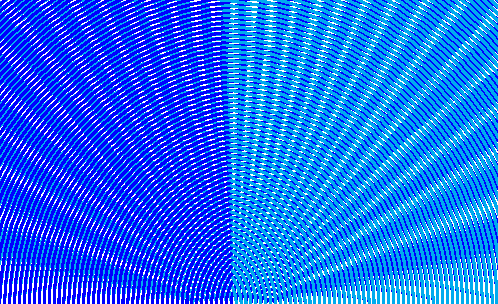
\includegraphics[width=85mm]{fig/A/cover.pdf} }
	
	%\maketitle %封面
	%\tableofcontents %目录
	%\frontmatter
	%\chapter{说明}

本书是在中小学通用教材物理编写组编的
《全日制十年制学校高中课本(试用本)物理》的基础上,
按照高中物理教学大纲较高要求的内容编写成的.编
写中吸收了几年来各地试用中的一些经验和意见.许多省市的中学教师和有关
高等院校的教师对本书征求意见稿提了有益的意见和建议.北京、安徽、江西、
河南、上海、天津、浙江、江苏、湖北、广东、山西、黑龙江等省市的教研室
和教育学院在本书编写过程中给予了大力支持.在此谨致谢意.

希望广大教师和研究中学物理教学的同志提出批评和修改建议.


\chapter{引言——怎样学好物理知识}

我们在初中学了两年物理,学习了一些物理概念,如质
量、重量、功、能、电流、电压、电阻等等;学习了一些物理定律,
如惯性定律、能的转化和守恒定律、欧姆定律、光的反射定律
等等;初步知道了一些物理理论,如分子论、电子论.这些概
念、定律、理论都是物理知识,正如我们在初中学习物理中体
会到的那样,物理知识是大们认识自然和改造自然的重要
武器.

经过几千年特别是近两三百年的积累,人类的物理知识
已经很丰富了,物理知识的应用已经很广泛了.在初中讲的
只是一些十分浅显的物理知识.为了适应把我国建设成为现
代化的,高度文明、高度民主的社会主义国家的需要,我们在
高中还要进一步学习物理知识.

    在高中,我们要加深对重要的物理知识的理解.例如,初
中讲了力是改变物体运动状态的原因,高中要进一步学习力
是怎样改变物体运动状态的;初中讲了闭合电路的一部分做
切割磁力线的运动时电路中要有感生电流,高中要进一步学
习感生电流的大小是怎样决定的等等.我们在高中还要扩
大物理知识的范围,例如,光到底是什么?常常听说的原子
能、激光等到底是怎么一回事?这些在初中没有讲到的物理
知识在高中都要讲到.在高中我们的物理知识将扩大和加
深.同时,我们学习物理知识的能力以及应用物理知识来分
析解决问题的能力也将得到提高.

    那么,在高中怎样进一步学好物理知识呢?

\subsection*{做好物理实验}
人类的物理知识是怎么得来的呢?想想
看,假使不研究物质的性质随温度的变化,人们能认识物态变
化的规律吗?假使不研究电流使磁针偏转等现象,人们能认
识电流周围存在着磁场吗?假使不研究反射光线和入射光线
的关系,人们能发现光的反射定律吗?整个物理学的发展史告
诉我们,人类的物理知识来源于实践,特别是来源于科学实验
的实践.

    我们学习物理知识的过程,跟人类探索物理知识的过程
有很多相似之处.因此,在高中迸一步学习物理的时候,必须
充分重视实践在学习物理知识中的重要意义,特别是要认真
做好实验.

    实验能够帮助我们形成正确的物理概念,增强观察物理
现象和分析物理问题的能力,加深对物理规律的理解,为了
做好实验,在每次实验之前,一定要明确实验的目的,弄懂它
的原理,了解所用仪器的性能,搞清楚实验的步骤;实验中要
认真观察现象,仔细记录必要的数据;实验后要对所得的数据
进行分析,作出合理的结论,必要时要进一步研究那些还不够
清楚的问题.这里,事先的准备工作特别重要.这是因为,我
们如果事前对实验目的和怎样达到这个目的的步骤都清楚
了,那么,在具体操作中,就能够自觉地有目的地把实验做好.
反之,如果事前不作好必要的准备,实验时只是按照别人拟定
的实验步骤去操作,观察时不知道把注意力集中到重要的现
象上,记录数据时不知道记下这些数据干什么,这样,实验虽
然做过了,收获却是很小的.为了做好实验,并从实验中得到
应有的收获,我们一定要作好事前的堆备,并在整个实验过程
中都要手脑并用.

    对老师的演示实验也要注意观察,并且要在老师的指导
下分析观察到的现象,得出应有的结论.还应努力创造条件
在课外多做一些简易实验.不做实验,不仔细观察物理现象,
是不能学好物理知识的.

\subsection*{学好物理概念和规律}

物理知识来源于实践,但实践的
经验并不就是物理知识.这跟房屋是由砖瓦等建筑材料组成
的,但建筑材料并不就是房屋一样.要把建筑材料变成房屋,
还需要人们进行修建房屋的劳动.与此相似,要从实践经验
中总结出物理知识,人们还必须进行分析、综合等抽象的思维
活动.例如,通过观察和实验,我们发现运动物体受到的阻力
越小,它的速度减小得越慢.但是,只有通过抽象思维,我们
才能得出物体不受外力时将保持匀速直线运动的结论.一般
说,人们在抽象出物理现象的共同属性后,就认识了有关的物
理概念,在抽象出物理现象的变化规律后,就发现了物理规
律.因此,我们必须充分注意在经验事实的基础上是经过怎
样的抽象思维而建立起理论知识的,才能学好物理概念和规
律.

物理概念和规律常常用数学公式来表示.例如密度的公
式$\rho=m/V$,功的公式$W=Fs$,欧姆定律的公式$I=U/R$,电
功率的公式$P=UI$等等,都是我们在初中学过的物理公式,
把概念和规律写成公式后,显得特别简单、明确,而且便于运
用它们来进行分析、推理、论证.物理规律还常常用函数图像
来表示.在初中学过的给晶体和非晶体加热时它们在熔解前
后温度随时间而变化的图线(图 \ref{fig_A_0-1}),就是一个例子.从图
中很容易看出晶体和非晶体在熔解时表现出不同的特点,晶
体在熔解时虽然继续受热但温度并不升高,非晶体就没有这
个特点.图像的突出优点是它很直观,而且比较容易直接根
据实验数据画出来.

\begin{figure}[htp]\centering 
\begin{subfigure}{0.46\linewidth}
	\centering
	\begin{tikzpicture}[>=stealth, thick]
		\draw [<->](0,3)--(0,0)--(4,0);
		\node at (.5,3) {温度};
		\node at (3.75,-.25) {时间};
		\draw (.5,.5)--(1.5,1.5)--(2.5,1.5)--(3.5,2.5);
		%\node at (2,-.75) {甲:晶体};
	\end{tikzpicture}
	\caption{晶体}\label{fig_A_0-1a}
\end{subfigure}
\hfil
\begin{subfigure}{0.46\linewidth}
	\centering
	\begin{tikzpicture}[>=stealth, thick]
		\draw [<->](0,3)--(0,0)--(4,0);
		\node at (.5,3) {温度};
		\node at (3.75,-.25) {时间};
		\draw (.5,.5) [bend left =15] to (3.5,2.5);
		%\node at (2,-.75) {乙:非晶体};
	\end{tikzpicture}
	\caption{非晶体}\label{fig_A_0-1b}
\end{subfigure}
\caption{物体受热时温度随时间而变化的图线
}\label{fig_A_0-1}
\end{figure}

    数学知识在物理学中的应用是十分重要的,但是我们却
不可以只从数学的角度来看待物理问题.对于物理概念,要
特别注意它的物理意义,对于物理规律,要特别注意它的适
用范围.

    有人总是认为水越深浮力就越大.其实,水对物体的浮
力等于物体排开的水的重量,跟物体在水中的深度没有关系,
发生这个错误的原因就在于对浮力的物理意义不清楚.有的
初学者从公式$R=U/I$得出结论说,导体的电阻跟加在导体
上的电压成正比,跟通过导体的电流强度成反比.实际上,电
阻是导体本身的属性,是由导体的长度、横截面积和材料决定
的,跟加在导体上的电压和通过导体的电流强度无关.这个
错误就是由于没有搞清楚电阻的物理意义,错误地理解公式
造成的.这些例子以及同学们自己也可以举出的类似的例子
说明,理解概念的物理意义是多么重要.

    物理规律一般都有一定的适用范围.例如,弹簧的伸长
只有在一定的限度内才跟所受的拉力成正比,超出这个限度,
伸长就不跟拉力成正比了,欧姆定律对金属导体是正确的,
对液体导电也适用,对气体导电就不成立了.物理规律不能
随意应用到它的适用范围之外去.例如,机械能在只有动能
和势能发生相互转化时才是守恒的.飞机起飞、火车制动、大
炮发射炮弹的时候,机械能都跟其他形式的能发生相互转化、
这时总的能量是守恒的,但机械能并不守恒.在这些情况下
就不能用机械能守恒定律来分析讨论问题,否则就会得到错
误的甚至荒谬的结果.所以,学习物理规律时,知道它的适用
范围是非常重要的.

    在高中,我们对物理概念和规律的讨论,要比在初中深入
得多,应用物理概念和规律来进行分析、推理和论证的机会也
很多.我们必须注意掌握物理概念和规律的物理意义和适用
范围,这样才能学懂学好物理知识.如果忽视这一要点,只去
死背定义,硬记公式,那是不可能学好物理知识的.


\subsection*{做好练习}

做练习是学好物理知识的必不可少的环节.
认真做好练习,可以加深对所学知识的理解,发现自己知识中
的薄弱环节而去有意识地加强它,逐步培养自己的分析解决
问题的能力,逐步树立解决实际问题的自信心.

物理练习有多种形式,如问答题、实验题、计算题等.怎样才能做好练习,不能一概而论,这里只能初步说明做好物理
练习一般需要注意的几个问题,作为入门的指引.

    我们知道,要处理好一件事情,首先是要把情况摸清楚.
做练习也是这样,先要仔细审题,弄清楚题中叙述的物理过
程.譬如有一道关于物体做机械运动的题,就要先弄清楚物
体是做匀速运动还是变速运动,它原来是静止的,还是本来就
在运动,运动轨迹是直线还是曲线,等等.把物理过程弄清楚
以后,要进一步明确哪些条件是已经知道的,什么是要解决的
问题即所求的答案.这样我们才有一个可靠的出发点.

    在弄清题意之后,再根据题中叙述的物理过程、已知条件
和所求答案来确定应该运用哪些物理规律.这是做好练习的
十分重要的而又往往被初学者忽视的一步.只有经过认真的
分析思考,把应该运用的物理规律找准了,我们才能有把握地
解决问题.否则就可能流于乱套公式,做对了不知道是怎么
对的,做错了也不知道是怎么错的.这样,即使做了很多练
习,也是收不到应有效果的.

    在找出了应该运用的物理规律之后,最后的工作就是利
用这些规律来建立已知条件和所求答案之间的关系,从而求
出答案.这个关系有时比较简单,容易看出来,有时比较复
杂,要逐步去寻找.对于比较复杂的问题怎样去逐步找出已
知条件和所求答案的关系,我们将在以后各章中结合例题来
具体说明.对得到的答案,还应该根据实际情况考虑它是否
合理.譬如所得答案是一个人有几吨重,飞机的速度只有几
厘米每秒,这显然是不合理的.如果发生这种情况,就要认真
检查什么地方出了错.

    做好练习的目的,是为了掌握所学的知识,培养我们运用
所学知识分析和解决问题的能力.希望同学们在做练习中,
既要肯于动脑筋,又要善于动脑筋,这样才能把物理知识真正
学到手,并培养起我们的能力来.不动脑筋,乱套公式,死记
类型,机械模仿,都不能达到做好练习的目的.为了掌握知
识,需要做一定数量的练习,但是,如果误以为学物理就是做
题,既不复习老师讲课的内容,也不阅读教材,就盲目地去找
过多的难题来做,同样不能达到做好练习的目的.
这些错误办法无助于我们学好本领,增长才干,一定要坚决摒弃.



 %引言
	%\mainmatter
	
	
	%正文内容
	%\chapter{力}\label{chapter-force}

    现在我们开始学习力学知识.力学所要解决的中心课题
是力和物体运动的关系.这一章学习有关力的知识,下一章
学习怎样描述物体的运动.有了这两章的知识淮备,到第三
章就可以学习力和物体运动的关系了.

    在这一章里,我们要在复习初中所学知识的基础上,进一
步学习力的知识,以加深和扩大我们对力的理解.研究力学
问题常常要分析物体的受力情况.这一章里要介绍怎样分析
物体的受力情况,希望同学们初步学会分析方法,并在以后的
学习中逐步熟悉它,掌握它.最后,我们还要在学习力的合成
与分解的基础上,学习矢量的概念和矢量运算的特殊性.


\section{力} 
    人们对力的认识,最初是从日常生活和生产劳动中得到
的,是和人力相联系的.用手推动小车,提起重物,拉长或压
缩弹簧,肌肉会感到紧张,我们就说,人对小车、重物、弹簧用
了力,后来人们把力的概念加以扩展,把凡是能和人力起相
同效果的作用都叫做力.机车牵引列车前进,机车对列车施
加了力.汽锤锻打工件,汽锤对工件施加了力.这样,人们建
立了这样的认识:\textit{力是物体对物体的作用} .

一个物体受到力的作用,一定有另一个物体施加这种作
用.前者是受力物体,后者是施力物体,只要有力发生,就一
定有受力物体和施力物体.有时为了方便,只说物体受到了
力,而没有指明施力物体,但施力物体一定是存在的.

    力是有大小的.我们在初中学过,力的大小可以用测力
计来测量.在国际单位制中力的单位是\textbf{牛顿} ,简称牛,国际符
号是N,日常生活和生产中常用的力的单位是千克力,牛顿
和千克力的关系是:1千克力$=9.8$牛.

    力不但有大小,而且有方向.物体受到的重力是竖直向
下的,物体在液体中受到的浮力是竖直向上的,力的方向不
同,它的作用效果也不同.用力拉弹簧,弹簧就伸长;用反方
向的力压弹簧,弹簧就缩短.
作用在运动物体上的力,如果方
向与运动方向相同,将加快物体的运动;如果方向与运动方向
相反,将阻碍物体的运动.可见,要把一个力完全表达出来,
除了说明力的大小外,还要指明力的方向.

为了直观地说明力的作用,常常用一根带箭头的线
段来表示力.线段是按一定比
例(标度)画出的,它的长短表
示力的大小,它的指向表示力
的方向,箭头或箭尾表示力的
作用点,箭头所沿的直线叫做
力的作用线.这种表示力的方
法,叫做\textbf{力的图示} .图 ~\ref{fig_A_1-1}  中表示的是作用在小车上的100牛
的力.

\begin{figure} [htp]\centering
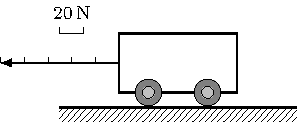
\includegraphics{fig/A/1-1.pdf} 
\caption{图中的虚线表示力的作用线} \label{fig_A_1-1} 
\end{figure} 

我们从初中开始学习物理以来,见过的力的名称已经相当多了.各种力可以用不同的方法来分类.
一种是根据力的性质来分类的,如重力、弹力、摩擦力、分子力、电磁力等
;另一种是根据力的效果来分类的,如拉力、压力、支持力、
动力、阻力等等.拉力、压力、支持力实际上都是弹力,只是效
果不同.不论是什么性质的力,只要效果是加快物体的运动,
就可以叫它为动力;效果是阻碍物体的运动,就可以叫它为阻
力.今后我们还会遇到根据效果来命名的力的名称.

    从力的性质来看,力学中经常遇到的有重力、弹力、摩擦
力.下面几节就分别介绍这三种力.


\section{重力} 
    地球上一切物体都受到地球的吸引作用.这种由于地球
的吸引而使物体受到的力叫做\textbf{重力} .重力也常常叫做\textbf{重量} .

    重力不但有大小,而且有方向.悬挂物体的绳子,静止时
总是竖直下垂的.自由落向地面的物体,总是竖直下落的,可
见重力的方向是竖直向下的.物体所受的重力的大小跟物体
的质量成正比,质量越大,所受的重力越大.1千克质量的物
体所受的重力是1千克力,即9.8牛;2千克质量的物体所受
的重力是2千克力,即$2\times 9.8$牛等等,把物体挂在绳子上,
物体静止时拉紧悬绳的力,大小等于物体所受的重力.把物
体放在静止的水平支持物上,物体压在水平支持物上的力,大
小也等于物体所受的重力.

    一个物体的各部分都要受到地球对它的作用力,我们可
以认为重力的作用集中于一点,这一点叫做物体的\textbf{重心} .如
图 \ref{fig_A_1-2} 那样用手指支持一根铅
笔,我们可以找到一个位置,使
铅笔水平地支持在手指上,手
指上方铅笔上的$C$点就是铅笔
的重心.这时铅笔受到两个力:
竖直向上的手指的支持力$N$,
竖直向下的重力$G$.这两个力大小相等方向相反,而且作用
在同一直线上,从初中学过的二力平衡条件知道,这时铅笔保
持平衡.如果重心$C$不在手指的正上方,支持力$N$和重力$G$,
将不在同一直线上,铅笔就不能保持平衡了.
\begin{figure} [htp]
\centering
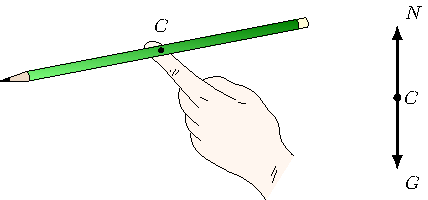
\includegraphics{fig/A/1-2.pdf} 
\caption{} \label{fig_A_1-2} 
\end{figure} 

    质量均匀分布的物体(均匀物体),重心的位置只跟物体
的形状有关.有规则形状的均匀物体,它的重心就在几何中
心上.例如,均匀直棒的重心在棒的中点,均匀球体的重心在
球心,均匀圆柱体的重心在轴线的中点(图 \ref{fig_A_1-3} ).

 \begin{figure} [htp]\centering
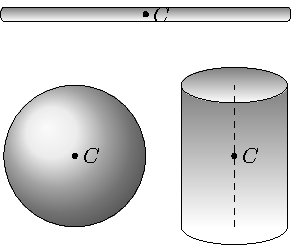
\includegraphics{fig/A/1-3.pdf} 
\caption{} \label{fig_A_1-3} 
 \end{figure} 

    不均匀物体的重心的位置,除跟物体的形状有关外,还跟
物体内质量的分布有关.载重汽车的重心随着装货多少而不
同,起重机的重心随着提升重物的重量和高度而变化.

    用简单的实验方法可以求出形状不规则或者质量不均匀
的薄板状物体的重心.如图~\ref{fig_A_1-4} 所示,先在$A$点把物体悬挂
起来,当物体处于平衡时,它所受的重力跟悬绳的拉力在同一
直线上,也就是说,重心一定在通过$A$点的竖直线$AB$上.然
后,在$D$点把物体悬挂起来,同样可以知道,重心一定在通过
$D$点的竖直线$DE$上.$AB$和$DE$的交点$C$就是物体的重心.


\begin{figure} [htp]
\centering
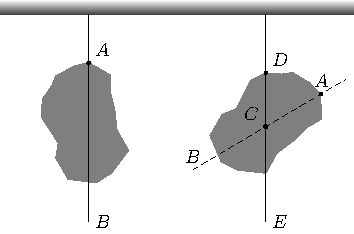
\includegraphics{fig/A/1-4.pdf} 
\caption{} \label{fig_A_1-4} 
\end{figure} 

\section{弹力} 
被拉长或压缩的弹簧对跟它接触的小车发生力的作用,
可以使小车运动起来(图~\ref{fig_A_1-5}).
被弯曲的细木棍或细竹竿对
跟它接触的圆木发生力的作用,可以把圆木推开(图~\ref{fig_A_1-6}).
物体的伸长、缩短、弯曲等等,总之物体的形状或体积的改变,叫
做形变.上面的例子说明,发生形变的物体,由于要恢复原
状,对跟它接触的物体会产生力的作用,这种力叫做\textbf{弹力} .

\begin{figure} [htp]
	\centering
	\begin{subfigure} {0.48\linewidth} 
		\centering
		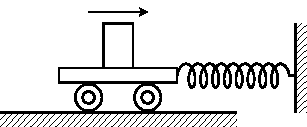
\includegraphics{fig/A/1-5a.pdf} 
		\caption{被拉长的弹簧使小车向右运动} \label{fig_A_1-5a} 
	\end{subfigure} 
	\hfill 
\begin{subfigure} {0.48\linewidth} 
	\centering
	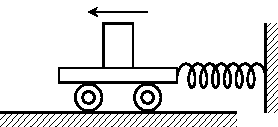
\includegraphics{fig/A/1-5b.pdf} 
	\caption{被压缩的弹簧使小车向左运动} \label{fig_A_1-5b} 
\end{subfigure} 
\caption{} \label{fig_A_1-5} 
\end{figure} 

\begin{figure} [htp]
\centering
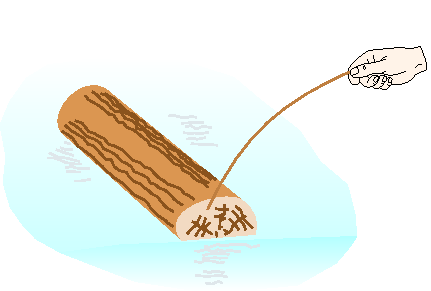
\includegraphics{fig/A/1-6.pdf} 
\caption{被弯曲的细木棍把圆木推开} \label{fig_A_1-6} 
\end{figure} 

    地球对物体产生重力,并不需要地球和物体直接接触.弹
力则不同,它只有在物体直接接触并产生形变的时候才能产
生,把一本书放在泡沫塑料上(图 \ref{fig_A_1-7} ),书把泡沫塑料压弯,
被压弯的泡沫塑料要恢复原状,产生向上的弹力,这就是它对
书的支持力.把一个物体挂在弹簧上,物体把弹簧拉长,被
拉长的弹簧要恢复原状,产生向上的弹力,这就是它对物体的
拉力.
\begin{figure} [htp]
\centering
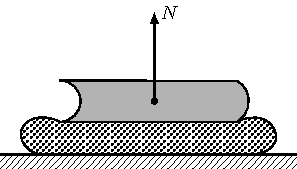
\includegraphics{fig/A/1-7.pdf} 
\caption{} \label{fig_A_1-7} 
\end{figure} 

    不仅泡沫塑料、弹簧等能够发生形变,任何物体都能够发
生形变,不能发生形变的物体是不存在的.不过有的形变比
较明显,直接可以看得见;有的形变极其微小,要用仪器才能
显示出来.把书放在桌面上,书压桌面,使桌面和书都发生极
其微小的形变.发生形变的书要恢复原状,对桌面产生向下
的弹力,这就是书对桌面的压力.发生形变的桌面要恢复原
状,产生向上的弹力,这就是桌面对书的支持力.\textit{凡是支持物体对物体的支持力,
都是支持物因为发生形变而对物体产生弹力;支持力的方向总是垂直于支持面并指向
被支持的物体} (图 \ref{fig_A_1-8} ).
把电灯挂在电线上,电灯拉紧电线,使电灯和电线
都发生极其微小的形变,发生形变的电灯要恢复原状,对电
线产生向下的弹力,这就是电灯对电线的拉力.发生形变的
电线要恢复原状,产生向上的弹力,这就是电线对电灯的拉
力.\textit{凡是一根线(或绳)对物体的拉力,都是这根线(或绳)因
为发生形变而对物体产生的弹力;拉力的方向总是指向线收
缩的方向} (图 \ref{fig_A_1-9} ).

\begin{figure} [htp]\centering
	\begin{subfigure} {0.46\linewidth} 
		\centering
		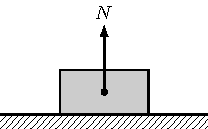
\includegraphics{fig/A/1-8a.pdf} 
		\caption{} \label{fig_A_1-8a} 
	\end{subfigure} 
	\hfil
\begin{subfigure} {0.46\linewidth} 
	\centering
	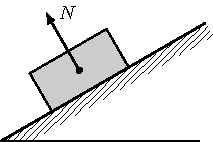
\includegraphics{fig/A/1-8b.pdf} 
	\caption{} \label{fig_A_1-8b} 
\end{subfigure} 
\caption{支持力的方向} \label{fig_A_1-8} 
\end{figure} 

\begin{figure} [htp]\centering
\begin{subfigure} {0.46\linewidth} 
	\centering
	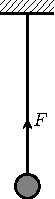
\includegraphics{fig/A/1-9a.pdf} 
	\caption{} \label{fig_A_1-9a} 
\end{subfigure} 
\hfil
\begin{subfigure} {0.46\linewidth} 
	\centering
	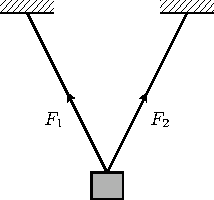
\includegraphics{fig/A/1-9b.pdf} 
	\caption{} \label{fig_A_1-9b} 
\end{subfigure} 
\caption{线的拉力的方向} \label{fig_A_1-9} 
\end{figure} 

\section*{阅读材料:显示微小形变的装置} 


图 \ref{fig_A_1-10} 是一种显示微小形变的装置,它可以把微小形变
“放大”到可以直接看出来.在一张大案子上放两个平面镜$M$
和$N$,让一束光线依次被这两面镜子反射,最后射到一个刻
度尺上,形成一个光点,只要用力压桌面,镜子就要向箭头所
示的方向倾斜. 由于两面镜子之间的距离较大,光点就会在
刻度尺上有明显的移动,而把桌面的形变显示出来.

    这个实验并不难做,希望同学们在教师指导下做一做,用
手压一下桌面,或者在桌面上放一个物体,看看光点是否发生
明显的移动.这个实验可以使你看到放在桌面上的一本书确
实会使桌面发生形变.

    在物理学实验中常常需要把微小的效应“放大”而显示出
来,在今后的学习中,希望同学们注意这一类实验的设计.

\begin{figure} [htp]
\centering
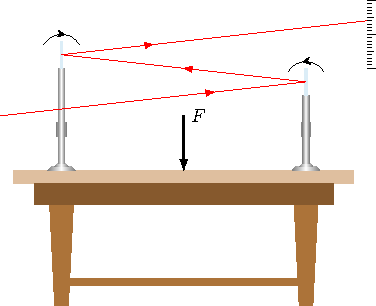
\includegraphics{fig/A/1-10.pdf} 
\caption{显示微小形变的装置} \label{fig_A_1-10} 
\end{figure} 

\subsection*{练习一} 
\begin{enumerate} 
\item  举出几个实例来说明力是物体对物体的作用.
\item 放在水平面上的物体(图 \ref{fig_A_1-8a} )受到几个力的作用?
  各是什么物体对它的作用,是哪种力?画出物体受力的示意
  图.
\item 用一根绳子把小球挂在天花板上(图 \ref{fig_A_1-9a} ),小球受
  到几个力的作用?各是什么物体对它的作用,是哪种力?画出
  小球受力的示意图.
\item 用两根绳子把物体挂在天花板上(图 \ref{fig_A_1-9b} ),这个物
  体受到几个力的作用?各是什么物体对它的作用,是哪种力?
  画出物体受力的示意图.
 \item 找一个薄板状的物体,用书中所讲的悬挂方法求出
  这个物体的重心.
 \item 放在水平桌面上的两个小球,它们靠在一起但不互
相挤压,它们之间有弹力作用吗?为什么?
\item 用下面的简单装置也可以显示微小形变.找一个大
玻璃瓶,装满水,塞上中间插有细管的瓶塞.用手按压玻璃瓶,
细管中的水面就上升;松开手,水面又降回原处.这说明玻璃瓶
遇到按压时发生弹性形变.实际做一下这个实验.
\end{enumerate} 

\section{胡克定律} 
力的大小跟形变的大小有关系,形变越大,弹力也越
大;形变消失,弹力就随着消失.对于拉伸(或压缩)形变来说,
伸长(或缩短)的长度越大,产生的弹力就越大,弹簧伸长或
缩短的长度越大,弹力就越大,这是我们从经验中都知道的.
把一个物体挂在悬线上,物体越重,把悬线拉得越长(实际上
还是看不出来),悬线的拉力也越大,物体发生弯曲时产生的
形变叫做弯曲形变.对于弯曲形变来说,弯曲得越厉害,产生
的弹力就越大.把弓拉得越满,箭就射出得越远,把一个物
体放在支持物上,物体越重,支持物弯曲得越厉害,支持力就
越大.还有一种叫做扭转形变,在金属丝的下面挂一个横
杆,用力扭这个横杆,金属丝就发生扭转形变(图 \ref{fig_A_1-11} ).放
开手,发生扭转形变的金属丝产生的弹力会把横杆扭回来.金
属丝的扭转角度越大,弹力就越大.

\begin{figure} [htp]\centering
\begin{subfigure} {0.32\linewidth} 
	\centering
	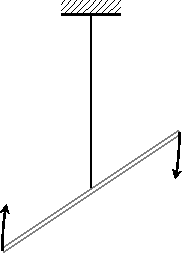
\includegraphics{fig/A/1-11a.pdf} 
	\caption{} \label{fig_A_1-11a} 
\end{subfigure} 
\hfil
\begin{subfigure} {0.32\linewidth} 
	\centering
	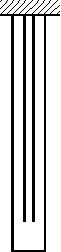
\includegraphics{fig/A/1-11b.pdf} 
	\caption{} \label{fig_A_1-11b} 
\end{subfigure} 
\hfil
\begin{subfigure} {0.32\linewidth} 
	\centering
	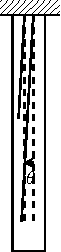
\includegraphics{fig/A/1-11c.pdf} 
	\caption{} \label{fig_A_1-11c} 
\end{subfigure} 

\caption{甲图表示用扭横杆的办法使金属丝发生扭
转形变.乙图是放大了的未发生扭转形变
的金属丝的示意图.丙图是放大了的发生
扭转形变的金属丝的示意图,$\theta$角可以用
来表示扭转形变的大小} \label{fig_A_1-11} 
\end{figure} 



    定量地研究各种形变中弹力和形变的关系比较复杂,我
们经常遇到的是弹簧的拉伸(或压缩)形变.实验表明:\textit{弹簧
弹力的大小$f$和弹簧伸长(或缩短)的长度$x$成正比.} 
写成公式就是
\[f=kx\]
其中$k$是比例常数,叫做弹簧的\textbf{倔强系数} .倔强系数是一个
有单位的量.在国际单位制中,$f$的单位是牛,$x$的单位是
米,$k$的单位是牛/米.倔强系数在数值上等于弹簧伸长(或
缩短)单位长度时的弹力.倔强系数跟弹簧的长度、弹簧的材
料、弹簧丝的粗细等等都有关系.弹簧丝粗的硬弹簧比弹簧
丝细的软弹簧倔强系数大.对于直杆和线的拉伸(或压缩)形
变,也有上述正比关系,这个规律是英国科学家胡克发现的,
叫做\textbf{胡克定律} .

    胡克定律有它的适用范围.物体的形变过大,超出一定
限度,上述正比关系将不再适用,这时即使撤去外力,物体也
不能完全恢复原状.这个限度叫做\textbf{弹性限度} .胡克定律在弹
性限度内适用.弹性限度内的形变叫做\textbf{弹性形变} .本书中提
到的形变,除非特别指明,一般是指弹性形变.

\subsection*{练习二} 
\begin{enumerate} 
\item 把一个重量为2牛的物体挂在弹簧上,物体静止时受
到的弹簧的弹力有多大?为什么?
\item 把重量相同的两个物体分别挂在两根不同的弹簧
上,一根弹簧伸长的长度小,另一根伸长的长度大,哪根弹簧
的倔强系数大?
\item 一根弹簧的倔强系数是100牛/米,伸长的长度为2厘
米时,弹簧的弹力有多大?另一根弹簧的倔强系数是2000
牛/米,缩短的长度为3厘米时,弹簧的弹力有多大?
\item 一根弹簧,不挂物体时长15厘米,挂上0.5千克的物
体时长18厘米.这根弹簧的倔强系数有多大?
\end{enumerate} 

\section{摩擦力} 
    摩擦力也是发生在两个互相接触的物体之间.当一个物
体在另一个物体表面上做相对滑动的时候,要受到另一个物
体阻碍它运动的力,这种力叫做滑动摩擦力.滑动摩擦力的
方向总跟接触面相切,并且跟物体的相对运动的方向相反(图
 \ref{fig_A_1-12} ).实验表明:\textit{滑动摩擦力跟压力成正比
也就是跟一个物体对另一个物体表面的垂直作用力成正比.} 
用$f$表示滑动摩擦力的大小,用$N$表示压力的大小,那么
\[f=\mu N,\]
\begin{figure} [htp]\centering
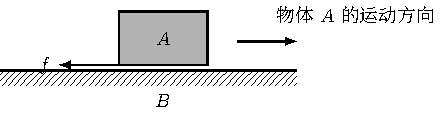
\includegraphics{fig/A/1-12.pdf} 
\caption{滑动摩擦力$f$的方向.为了清楚地表示摩
擦力,此图把相互接触的两个物体画得隔
开一些.
} \label{fig_A_1-12} 
\end{figure} 
其中$\mu$是比例常数,叫做\textbf{滑动摩擦系数} .滑动摩擦系数是由
制成物体的材料决定的,材料不同,两物体间的滑动摩擦系数
也不同.滑动摩擦系数还跟接触面的粗糙程度有关.在相同
的压力下,滑动摩擦系数越大,滑动摩擦力就越大.滑动摩擦
系数是两个力的比值,没有单位.表 \ref{tab_A_1-1} 列出了在通常情况下
几种材料间的滑动摩擦系数.

\begin{table} [htp]\centering
\caption{几种材料间的滑动摩擦系数} \label{tab_A_1-1} 
\begin{tabular} {cc} 
\hline
材料   &  滑动摩擦系数\\
\hline
钢—钢     & 0.25 \\
木—木   & 0.30 \\
木—金属   &  0.20\\
皮革—铸铁   &  0.28\\
钢—冰   &  0.02\\
木头—冰   &  0.03\\
橡皮轮胎—路面(干)   &  0.71\\
\hline
\end{tabular} 
\end{table} 

    除了滑动摩擦,还有滚动摩擦.滚动摩擦是一个物体在
另一个物体表面上滚动时产生的摩擦.滚动摩擦比滑动摩擦
小得多,滚动轴承就是利用滚动摩擦小的事实制成的.

    滑动摩擦和滚动摩擦都是一个物体在另一个物体表面上
有相对运动的时候发生的.那么,互相接触的两个物体处于
相对静止的时候,是不是也可以发生摩擦呢?我们用不大的力
来推桌子,虽然桌子应该沿着力的方向运动,有相对于地板运
动的趋势,但并没有把桌子推动,就是因为桌腿跟地板之间发
生了摩擦.这个摩擦力和推力都作用在桌子上,它们的大小
相等,方向相反,彼此平衡,因此桌子保持不动.这时所发生
的摩擦叫静摩擦,静摩擦力的方向总跟接触面相切,并且跟
物体相对运动趋势的方向相反.

    逐渐增大对桌子的推力,如果推力还不够大,桌子仍旧保
持不动,静摩擦力跟推力仍旧彼此平衡.可见静摩擦力随着
推力的增大而增大.但是静摩擦的增大有一个限度,静摩擦
力的最大值叫最大静摩擦力.推力超过最大静摩擦力,就可
以把桌子推动了.最大静摩擦力等于使桌子开始运动所需的
最小推力.


\section*{阅读材料:力的种类} 
    在力学中经常遇到的有重力、弹力和摩擦力,以后在热学
中要遇到分子力,在电学中要遇到电磁力.在课文中我们曾
经提到,重力、弹力、摩擦力、分子力、电磁力等是根据力的性
质来分类的,即认为它们是属于不同性质的力,其实这种认
识只是反映了人们对力的认识的一个阶段.随着科学的发展,
人们对力的探索已经从宏观物体进入到原子、分子的微观领
域,因而对力的认识也进一步深化了.现代科学研究告诉我
们,通常见到的重力、弹力、摩擦力、分子力、电磁力等都可以
归结为两种基本的相互作用,即万有引力和电磁力.

    关于万有引力,我们将在第\ref{chapter-law-of-universal-gravitation}章学习.万有引力是由于物
体具有质量而在物体之间产生的一种相互作用.这种力普遍
存在于宇宙万物之间.在宇宙天体之间,在宏观物体之间,在
原子、分子等粒子之间,都存在着这种相互作用.两个通常物体
之间的万有引力极其微小,我们觉察不到它,可以不予考虑.但
是,在天体系统中万有引力却起着决定性的作用.在天体中质
量还算很小的地球对其他物体的万有引力已经具有巨大影
响,它把人类、大气和所有地面物体束缚在地球上,它使月球
和人造地球卫星绕地球旋转而不能离去.重力就是地面附近
的物体由于受到地球的万有引力而产生的.太阳系中的八大
行星绕太阳旋转而不离去,是由于万有引力的作用.银河系里
的球状星团——由上百万个恒星聚在一起并呈球状的恒星集
合体——聚集不散,也是由于万有引力的作用.

    电磁力是存在于电荷之间的一种相互作用.静止电荷之
间有电力,运动电荷之间除了电力外还有磁力.电力和磁力
是有联系的,常常总称为电磁力.我们知道,原子是由带正电
的原子核和绕核旋转的带负电的电子组成的,分子是由原子
组成的.原子或分子本身能够形成,是由于电磁力的作用.分
子之间的电磁力就构成了我们通常所说的分子力.我们所看
到的多种多样的宏观物体是由原子或分子组成的,它们能聚
集不散而且使物体构成一定的形态,就是由于原子或分子之
间的电磁相互作用.从微小的原子到通常的物体,正是电磁
力把物质结合在一起的.

    当我们使物体发生形变的时候,物体中原子或分子之间
的距离发生改变,原子或分子之间的电磁力要反抗物体发生
形变,这就形成了我们通常所说的弹力.摩擦力也可以归结
为电磁力.虽然从原子或分子之间的电磁力来完满地解释摩
擦力很为复杂,至今还没有一种很好的理论,但是大家公认摩擦
力说到底也还是电磁力的一种表现.

    我们看到,从宇宙天体到微小的原子,这中间只有两种基
本的相互作用:万有引力和电磁力.现代科学研究又深入一
步,深入到原子核内部,深入到研究质子、中子等粒子的相互
作用.人们在这个领域又发现了两种基本的相互作用,分别
叫做强相互作用和弱相互作用.这两种相互作用这里不再介绍了.

    这样,人类认识到在自然界中只存在四种基本的相互作
用:万有引力,电磁力,强相互作用,弱相互作用.小到比原
子还小的粒子,大到宇宙天体,其间表现出很不相同的多种多
样的相互作用,都可以用少数几种基本的相互作用来说明,这
是物理学的巨大胜利.然而人类的认识是没有止境的,今天
认为基本的相互作用只有四种,明天会不会统一成更少的几
种甚至一种相互作用呢?大物理学家、相对论的创立者爱因斯
坦(1879—1955),晚年致力于这方面的工作,企图把万有引力
和电磁力统一起来.现在有不少物理学家致力于这方面的研
究,企图把四种相互作用统一起来,并且取得了进展.这是物
理学的前沿阵地,物理学好像一座正在施工中的大厦,它已
经建筑得很壮观了,但还没有竣工,看来永远也不会竣工,更
壮观的还在后面.现在的青年学生,将来就可能成为修建这
座大厦的建筑师.

\subsection*{练习三} 
\begin{enumerate} 
\item  在东北的冬季伐木工作中,许多伐下的木料被装在
雪橇上,用马拉着在冰道上运出去.一个有钢制滑板的雪橇,
上面装着木料,共重$4.9\times 10^4$牛.在水平的冰道上,马要在水平
方向用多大的力才能够拉着雪橇匀速前进?

\item  用20牛的水平的力拉着一块重量是40牛的砖,可以
使砖在水平地面上匀速滑动.求砖和地面之间的滑动摩擦系
数.
\item  要使重量是400牛的桌子从原地移动,必须最小用
200牛的水平推力.桌子从原地移动以后,为了使它继续做匀
速运动,只要160牛的水平推力就行了.求最大静摩擦力和滑
动摩擦系数.如果用100牛的水平推力推桌子,这时静摩擦力
有多大?

\item  做下面的实验:用一根橡皮绳把书吊起来,当书静
止不动的时候,测出橡皮绳伸长的长度.把书放在桌子上,水
平拉橡皮绳,使书做匀速运动,再测出橡皮绳伸长的长度.设
橡皮绳伸长的长度跟外力成正比,根据测出的数据粗略地算
出书和桌面之间的滑动摩擦系数.
\end{enumerate} 


\section{牛顿第三定律} 
我们知道,力是物体对物体的作用,只要有力发生,就一
定要有受力物体和施力物体.施力物体是不是也要受到受力
物体给予它的力呢?力是物体间的单方面作用,还是物体间
的相互作用?

    用手拉弹簧,手的肌肉发生紧张(形变),同时弹簧也发生
形变,这时不但弹簧受到手的拉力,手也受到弹簧的拉力.坐
在椅子上用力推桌子,会感到桌子也在推我们,我们的身体要
向后移.在平静的水面上,在一只船上用力推另一只船,另一
只船也要推前一只船,两只船将同时向相反方向运动(图 \ref{fig_A_1-13} ).在水面上放两个软木塞,一个软木塞上放一个小磁铁,
另一个软木塞上放一个小铁条(图 \ref{fig_A_1-14} ),可以看到,由于小
磁铁和小铁条相互吸引,两个软木塞相向运动起来.地球和
地面上物体之间的作用也是相互的,地面上的物体受到地球
的吸引,即受到重力,地球也受到地面上的物体的吸引.

\begin{figure} [htp]\centering
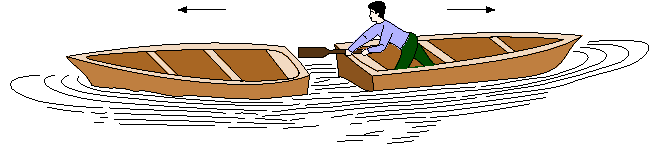
\includegraphics{fig/A/1-13.pdf} 
\caption{} \label{fig_A_1-13} 
\end{figure} 

\begin{figure} [htp]\centering
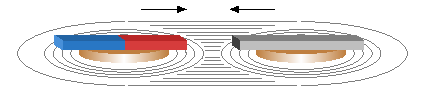
\includegraphics{fig/A/1-14.pdf} 
\caption{} \label{fig_A_1-14} 
\end{figure} 

观察和实验表明,两个物体之间的作用总是相互的,一
个物体对另一个物体有力的作用,后一个物体一定同时对前
一个物体有力的作用.\textit{力是物体与物体间的相互作用} .物体
间相互作用的这一对力,常常叫做\textbf{作用力} 和\textbf{反作用力} .把力
分成为作用力和反作用力并不是绝对的,我们可以把其中一
个力叫做作用力,另一个力就叫做反作用力.

    作用力和反作用力之间存在什么样的关系呢?

\begin{figure} [htp]\centering
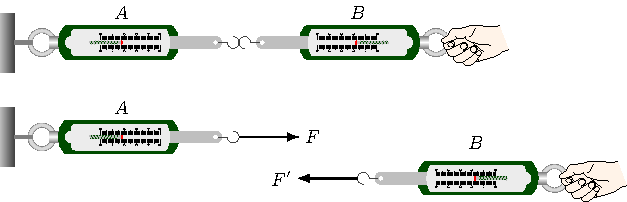
\includegraphics{fig/A/1-15.pdf} 
\caption{} \label{fig_A_1-15} 
\end{figure} 

    把两个弹簧秤$A$和$B$联结在一起(图 \ref{fig_A_1-15} ).用手拉弹
簧秤$A$,可以看到两个弹簧秤的指针同时移动.弹簧秤$B$的
读数指出弹簧秤$A$对它的作用力$F$的大小,而弹簧秤$A$的读
数指出弹簧秤$B$对它的反作用力$F'$的大小.可以看到,两个
弹簧秤的读数是相等的.改变手拉弹簧的力,弹簧秤的读数
也随着改变,但两个读数总相等,这说明作用力和反作用力
大小相等,方向相反.

    总结这类实验结果,得到结论:\textbf{两个物体之间的作用力和
反作用力总是大小相等,方向相反,作用在一条直线上.} 这就
是\textbf{牛顿第三定律} .

牛顿第三定律在生活和生产中应用很广泛.人走路时用
脚蹬地,脚对地面施加一个作用力,地面同时给脚一个反作用
力,使人前进.轮船的螺旋桨旋转时,用力向后推水,水同时
给螺旋桨一个反作用力,推动轮船前进.汽车的发动机驱动
后轮转动,由于轮胎和地面间有摩擦,车轮向后推地面,地面
给车轮一个向前的反作用力,使汽车前进.汽车的牵引力就
是这样产生的,如果把后轮架空,不让它跟地面接触,这时让
发动机驱动后轮转动,由于车轮不推地面,地面也不产生向前
推车的力,汽车就不能前进.

    我们在初中学过二力平衡:作用在同一物体上的两个力,
如果大小相等,方向相反,并作用在同一直线上,这两个力就
互相平衡,物体就保持原来的静止状态或匀速直线运动状态.
这种情况跟我们现在讲的物体间的相互作用力是不同的,作
用力和反作用力分别作用在不同的物体上,根本不存在相互
平衡的问题.这一点,在应用牛顿第三定律时要特别注意.


\subsection*{练习四} 
\begin{enumerate} 
\item  有人说“施力物体同时也一定是受力物体”,这句话
正确吗?用两三个实例来说明.

\item  地球的质量大约是$6\times 10^{24} $千克.地球对地面上质
量是1千克的石块的引力跟这个石块对地球的引力相比较,哪
个力大?根据牛顿第三定律,正确的答案是什么?

\item  用牛顿第三定律判断下列说法是否正确.
\begin{enumerate} 
\item  只有你站在地上完全不动,你和地球之间的相互作用
力才是一对大小相等方向相反的力.
\item  物体$A$静止在物体$B$上,$A$的质量是$B$的质量的100
倍,因此,$A$作用于$B$的力大于$B$作用于$A$的力.
\end{enumerate} 

\item  放在水平面上的物体(图 \ref{fig_A_1-8a} )受到两个力的作用.
这两个力的反作用力各作用在什么物体上?在这四个力中,哪
两对力是作用力和反作用力?哪两个力是相互平衡的力?
\item  挂在绳子(或弹簧)上的物体(图 \ref{fig_A_1-9a} )受到两个力
的作用.这两个力的反作用力各作用在什么物体上?在这四
个力中,哪两对力是作用力和反作用力?哪两个力是相互平衡
的力?
\item 从上述两题的解答中,试找出一对作用力和反作用
力跟两个相互平衡的力之间的区别.

\end{enumerate} 

\section{物体受力情况分析} 
    研究力学问题经常要分析物体的受力情况.分析物体受
力情况对于解决力学问题十分重要.怎样来分析物体受力情
况呢?下面先讨论几个具体例子.

    (1) \textbf{在水平面上的物体 }  一本书放在水平桌面上,书受
到两个力的作用.书由于受到地球的吸引而受到重力$G$,方
向竖直向下.书压在桌面上使桌面发生极微小的形变,发生
形变的桌面对书产生支持力$N$,方向竖直向上.书的受力图
如图 \ref{fig_A_1-16} 所示.由于书是静止在桌面上的,所以$G$和$N$是作
用在书上的相互平衡的力,它们大小相等方向相反.
\begin{figure} [htp]\centering
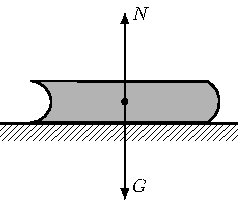
\includegraphics{fig/A/1-16.pdf} 
\caption{} \label{fig_A_1-16} 
\end{figure} 

    一个在水平面上运动的木块,运动越来越慢,最后停下
来,在这个过程中,木块受到几个力的作用?木块除了同样
受到重力$G$和支持力$N$的作用外,还受到滑动摩擦力$f$作
用,滑动摩擦力$f$的方向与木块运动的方向相反.木块的受
力图如图 \ref{fig_A_1-17} 所示.

\begin{figure} [htp]\centering
	\begin{minipage} [t]{0.48\textwidth} 
		\centering
		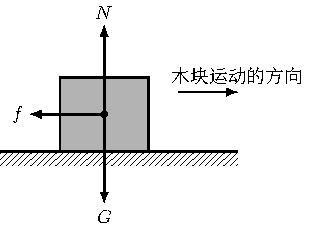
\includegraphics{fig/A/1-17.pdf} 
		\caption{} \label{fig_A_1-17} 
	\end{minipage} 
	\begin{minipage} [t]{0.48\textwidth} 
		\centering
		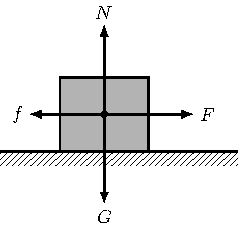
\includegraphics{fig/A/1-18.pdf} 
		\caption{} \label{fig_A_1-18} 
	\end{minipage} 
\end{figure} 

    木块其实还受到空气的阻力.空气阻力的方向也跟木块
运动的方向相反.空气阻力的大小跟物体的运动速度有关
系,速度越大,空气阻力越大.空气阻力的大小还跟物体的横
截面积和形状有关系,横截面积越大,空气阻力越大.木块的
横截面积较小,而且运动速度不大,在分析它的受力情况时,
空气阻力可以忽略不计.可是,在分析汽车、电车、火车的受
力情况时,空气阻力往往不能忽略不计,这时常把摩擦阻力和
空气阻力合在一起,一并加以考虑.

    如采用水平的绳拉着木块在水平面上运动,那么,木块除
了同样受到重力$G$、支持力$N$和滑动摩擦力$f$的作用外,还受
到绳的拉力$F$.木块一共受到四个力的作用,受力图如图 \ref{fig_A_1-18} 所示.

    在图 \ref{fig_A_1-17} 和图 \ref{fig_A_1-18} 所示的
情形里,木块沿着水平方向运动,
竖直方向的两个力$G$和$N$,跟木
块静止在水平面上的情形一样,仍旧是互相平衡的力.也就是说,重力$G$和支持力$N$大小相
等方向相反.


    (2) \textbf{在斜面上运动的物体 }  一个木块沿着光滑的斜面下
滑,它受到几个力的作用?木块受到重力$G$,方向竖直向下.
由于木块压斜面,斜面发生形变而对木块产生支持力$N$,方
向垂直于斜面并指向被支持的木块.木块受到这两个力的作
用,受力图如图 \ref{fig_A_1-19} 所示.

\begin{figure} [htp]\centering
	\begin{minipage} [t]{0.48\textwidth} 
		\centering
		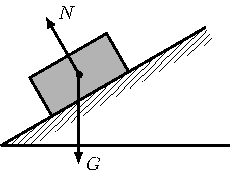
\includegraphics{fig/A/1-19.pdf} 
		\caption{} \label{fig_A_1-19} 
	\end{minipage} 
	\begin{minipage} [t]{0.48\textwidth} 
		\centering
		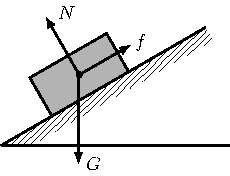
\includegraphics{fig/A/1-20.pdf} 
		\caption{} \label{fig_A_1-20} 
	\end{minipage} 
\end{figure} 


    如果斜面不是光滑的,那么,木块沿着斜面下滑时,除了
受到重力$G$和支持力$N$以外,还受到滑动摩擦力$f$的作用,它
的方向与木块的运动方向相反,沿着斜面向上.木块的受力
图如图 \ref{fig_A_1-20} 所示.


有人可能认为,木块既然沿着斜面下滑,它一定还受到一
个“下滑力”.我们知道,力是物体对物体的作用,力不能离开
物体而独立存在.木块所受的重力$G$、支持力$N$和滑动摩擦
力$f$,是木块周围的物体即地球和斜面施加给木块的.木块
周围再没有别的物体对它施加力的作用.因此,另外附加一
个“下滑力”,便是多余的.至于木块为什么下滑,同学们学到
后面就会明白了.

    从上述几个例子我们可以看出,分析物体的受力情况,首
先要明确被研究的对象,即明确我们是要分析哪个物体的受
力情况.明确了被研究的对象以后,把它从周围物体中隔离出
来,分析周围有哪些物体对它施加力的作用,它是什么性质的
力,力的大小和方向怎样,并把它们一一画在受力图上.这种
分析力的方法叫做\textbf{隔离法} .用隔离法分析力,既不要马虎从
事,随意丢掉任何一个力,也不要无中生有,脱离开力是物体
对物体的作用而凭空想出某个多余的力.至于被研究的物体
对周围其他物体的反作用力,一般可不予考虑;如果因问题的
需要而必须加以考虑,应该明确那是作用在其他物体上的力,
不要错加在被研究的物体上.

    物体的受力情况实际上往往是很复杂的,为了使问题简
化,往往可以略去某些次要因素,例如物体在光滑平面上运
动时,可以略去滑动摩擦力,物体的横截面积较小而且运动速
度不大时,可以不考虑空气阻力.根据所提问题的情况,略去
某些次要因素,这在物理学上是一种常用的研究方法,应该逐
渐熟悉它,掌握它.
分析物体受力情况,同学们做过一些练
习,有了一定经验以后,就能够根据具体情况自己判断哪些次
要因素可以忽略不计了.

\subsection*{练习五} 
    在下面各题中,在画受力图的时候,如果已知力的大小和
方向,要按照一定的标度做力的图示;如果未给出力的大小,
可以只画出力的方向.
\begin{enumerate} 
\item 竖直向上抛出的石块受到几个力的作用?水平抛出
的石块受到几个力的作用?竖直向下抛出的石块受到几个力
的作用?放开手,让石块自由下落,石块受到几个力的作用?分
别画出石块的受力图.不考虑空气阻力.

\item 一个物体沿着光滑的斜面滑下来,物体受到几个力
的作用?物体原来具有某一速度,它沿着光滑的斜面滑上去的
时候受到几个力的作用?分别画出物体的受力图.

    如果物体和斜面之间有滑动摩擦,受力情况又怎样?再分
别画出物体的受力图.

\item 雨滴下落的速度较大,空气阻力不能忽略不计.无
风的时候雨滴匀速竖直下落,雨滴受到几个力的作用?设雨滴
的重量是0.001牛,画出雨滴的受力图.

\item 用水平绳拉着木块在水平面上运动,木块的重量是
5牛,绳的拉力是10牛,滑动摩擦系数是0.3.画出木块的受力图.

\item 如图 \ref{fig_A_1-21} 那样用一根绳子$a$把物体挂起来,再用另一根
水平的绳子$b$把物体拉向一旁固定起来.这个物体受到几个力的
作用?画出物体的受力图.

\begin{figure} [htp]\centering
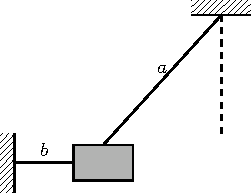
\includegraphics{fig/A/1-21.pdf} 
\caption{} \label{fig_A_1-21} 
\end{figure} 

\item  在图 \ref{fig_A_1-16} 中没有画出书对桌面的压力$N'$,把这个力
画出来,并回答下面的问题:
\begin{enumerate} 
\item 压力$N'$是什么性质的力?
\item 压力$N'$跟哪个力是一对作用力和反作用力?
\item 压力$N'$和重力$G$是不是作用在同一个物体上的力?
\item 在书静止地压在桌面上的情况下,压力$N'$和重力$G$的大小有什么关系?
\end{enumerate} 


\end{enumerate} 

\section{力的合成} 

    在大多数实际问题里,物体往往不只受到一个力,而是同
时受到几个力.一个物体受到几个力共同作用的时候,我们
常常可以求出这样一个力,这个力产生的效果跟原来几个力
共同产生的效果相同.一个力,如果它产生的效果跟几个力
共同产生的效果相同,这个力就叫做那几个力的\textbf{合力} ,求几
个力的合力叫做\textbf{力的合成} . 

\begin{figure} [htp]
\centering
\begin{subfigure} {1\linewidth} 
	\centering
	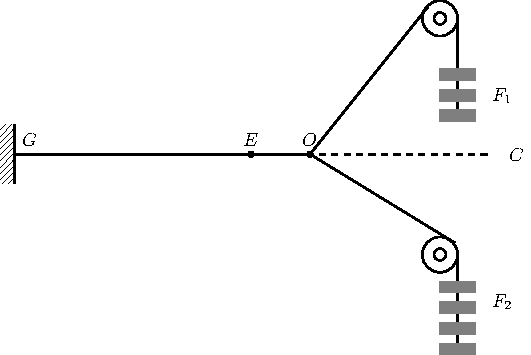
\includegraphics{fig/A/1-22a.pdf} 
	\caption{} \label{fig_A_1-22a} 
\end{subfigure} 
\begin{subfigure} {1\linewidth} 
	\centering
	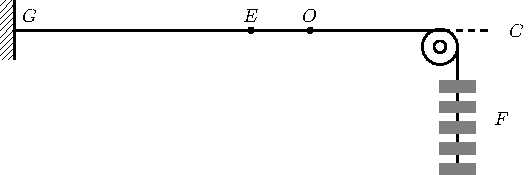
\includegraphics{fig/A/1-22b.pdf} 
	\caption{} \label{fig_A_1-22b} 
\end{subfigure} 
\begin{subfigure} {1\linewidth} 
	\centering
	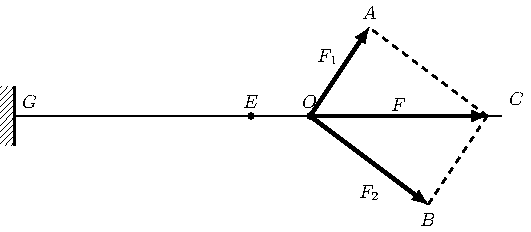
\includegraphics{fig/A/1-22c.pdf} 
	\caption{} \label{fig_A_1-22c} 
\end{subfigure} 
\caption{} \label{fig_A_1-22} 
\end{figure} 


    几个力如果都作用在物体的同一点,或者它们的作用线
相交于同一点,这几个力叫故\textbf{共点力} .现在我们先来研究作
用于物体某一点上的两个力的合成.

    图 \ref{fig_A_1-22a} 表示橡皮条$GE$在力$F_1$和$F_2$的共同作用下,
沿着直线$GC$伸长了$EO$这样的长度.图 \ref{fig_A_1-22b} 表示撤去$F_1$
和$F_2$,用一个力$F$作用在橡皮条上,使橡皮条沿着相同的直
线伸长相同的长度.力$F$对橡皮条产生的效果跟力$F_1$
和$F_2$
共同产生的效果相同,所以力$F$是力$F_1$
和$F_2$的合力.




    合力$F$跟力$F_1$
和$F_2$有什么关系呢?在力$F_1$
和$F_2$的方
向上各作线段$OA$和$OB$,根据选定的标度,可使它们的长度分
别表示力$F_1$和$F_2$的大小(图 \ref{fig_A_1-22c} ),以$OA$和$OB$为邻边
作平行四边形$OACB$,量出这个平行四边形的对角线$OC$的
长度,可以看出,根据同样的标度,合力$F$的大小和方向可以
用对角线$OC$表示出来.

    改变力$F_1$和$F_2$的大小和方向,重做上述实验,可以得到
同样的结论.

    可见,求两个互成角度的共点力的合力,可以用表示这两
个力的线段为邻边作平行四边形,这两个邻边之间的对角线
就表示合力的大小和方向,这叫做\textbf{力的平行四边形法则} .

    根据平行四边形对边平行而且相等的性质,力的平行四
边形还可以用更简单的作画法来代替.在图 \ref{fig_A_1-23a} 中$F$是
共点力$F_1$和$F_2$的合力.如图 \ref{fig_A_1-23b} 所示,从$O$点出发,把
代表$F_1$和$F_2$的线段$OA$、$AC$首尾相接地画出来,连接$O$和
$C$,从$O$指向$C$的线段就表示合力$F$的大小和方向.上述作
图法叫做\textbf{三角形法} .作三角形$OBC$(图 \ref{fig_A_1-23c} )同样可以求
出$F_1$和$F_2$的合力$F$.

\begin{figure} [htp]
	\centering
	\begin{subfigure} {1\linewidth} 
		\centering
		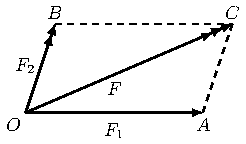
\includegraphics{fig/A/1-23a.pdf} 
		\caption{} \label{fig_A_1-23a} 
	\end{subfigure} 
	\begin{subfigure} {0.45\linewidth} 
		\centering
		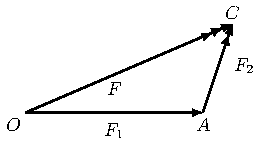
\includegraphics{fig/A/1-23b.pdf} 
		\caption{} \label{fig_A_1-23b} 
	\end{subfigure} 
	\begin{subfigure} {0.45\linewidth} 
		\centering
		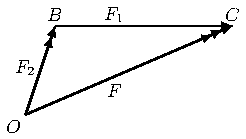
\includegraphics{fig/A/1-23c.pdf} 
		\caption{} \label{fig_A_1-23c} 
	\end{subfigure} 
	\caption{} \label{fig_A_1-23} 
\end{figure} 

    如果有两个以上的共点力作用在物体上,我们也可以应
用平行四边形法则或三角形法求出它们的合力:先求出任意
两个力的合力,再求出这个合力跟第三个力的合力,直到把所
有的力都合成进去,最后得到的合力就是这些力的合力.

\section{力的合成的计算} 
    合力的大小和方向,还可以利用公式来计算.图 \ref{fig_A_1-24} 中
的$OA$和$OB$分别表示两个力$F_1$和$F_2$,$OC$表示它们的合力
$F$,力$F_1$和$F_2$的夹角为$\theta$.

\begin{figure} [htp]
\centering
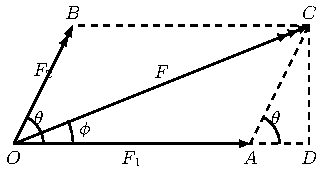
\includegraphics{fig/A/1-24.pdf} 
\caption{} \label{fig_A_1-24} 
\end{figure} 


    在三角形$OAC$中,根据余弦定理得到
\[\begin{split} 
F^2 & = F_1^2+F_2^2-2F_1F_2\cos(180^\circ -\theta)  \\
&= F_1^2+F_2^2+2F_1F_2\cos\theta
\end{split}  \]
所以合力的大小
\begin{equation}\label{eq-A-1.1}
F=\sqrt{F_1^2+F_2^2+2F_1F_2\cos\theta} 
\end{equation} 

    合力的方向可以用合力跟原来任一个力的夹角表示出
来.图中用$F$跟$F_1$的夹角$\phi$来表示,利用直角三角形$ODC$,
可以求出角$\phi$的正切:
\begin{equation}\label{eq-A-1.2}
\tan\phi =\frac{CD} {OD} =\frac{CD} {OA+AD} =\frac{F_2\sin\theta } {F_1+F_2\cos\theta} 
\end{equation} 




    根据 \eqref{eq-A-1.1} \eqref{eq-A-1.2} 两式,可以算出两个共点力的合力的大小和
方向,例如在运河两岸拉着一艘货船前进,两条绳对货船的
拉力都是$2\times 10^3$牛,两绳互成$45^\circ$角(图 \ref{fig_A_1-25} ).合力的大
小是:
\[\begin{split} 
F&= \sqrt{F_1^2+F_2^2+2F_1F_2\cos\theta} \\
&=\sqrt{(2\times 10^3)^2+(2\times 10^3)^2+2(2\times 10^3)^2\cos 45^{\circ} } \text{ 牛} \\
&=3.7\times 10^3\text{ 牛} 
\end{split}  \]
\[\begin{split} 
\tan\phi&= \frac{F_2\sin\theta } {F_1+F_2\cos\theta} \\
&= \frac{2\times 10^3\times \sin 45^{\circ} } {2\times 10^3+2\times 10^3\times \cos 45^{\circ} }   \\
&=0.4142\\
\phi &= 22^{\circ}  30'
\end{split}  \]

\begin{figure} [htp]
\centering
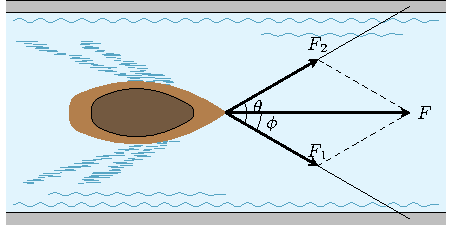
\includegraphics{fig/A/1-25.pdf} 
\caption{} \label{fig_A_1-25} 
\end{figure} 

    由于$F_1=F_2$,利用力的平行四边形,由几何方法容易证
明合力$F$的方向沿着力$F_1$和$F_2$的夹角平分线的方向.这跟
应用公式 \eqref{eq-A-1.2} 算出夹角$\phi$来表示合力的方向是一致的.

    现在我们来讨论,力$F_1$和$F_2$的大小一定的时候,合力$F$
的大小跟两个力的夹角$\theta$的关系.

\begin{figure} [htp]
\begin{subfigure} {0.46\linewidth} 
	\centering
	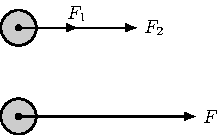
\includegraphics{fig/A/1-26a.pdf} 
	\caption{} \label{fig_A_1-26a} 
\end{subfigure} 
\hfil
\begin{subfigure} {0.46\linewidth} 
	\centering
	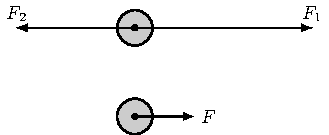
\includegraphics{fig/A/1-26b.pdf} 
	\caption{} \label{fig_A_1-26b} 
\end{subfigure} 
\caption{} \label{fig_A_1-26} 
\end{figure} 

    当两个力的方向相同时(图 \ref{fig_A_1-26a} ),$\theta =0^\circ$,$\cos 0^\circ=1$,
所以$F=F_1+F_2$,合力的大小等于两个力的大小之和,合力的
方向跟两个力的方向相同.

    当两个力的方向相反时(图 \ref{fig_A_1-26b} ),$\theta =180^\circ$,$\cos 180^\circ=-1$,
所以$F=F_1-F_2$,合力的大小等于两个力的大小之差,
方向跟两个力中较大的那个力的方向相同.如果力$F_1$和$F_2$
的大小相等,合力就等于零.

    当$F_1$和$F_2$的夹角$\theta$在$0^\circ$到$180^\circ$之间时,$\theta$越大,
$\cos\theta$的值越小,合力就越小,而且合力的方向也随着夹角$\theta$的变化
而变化.


\subsection*{练习六} 
\begin{enumerate} 
\item 两个力的合力总大于原来的每一个力,这话对吗?为
什么?

\item 有两个力$F_1$和$F_2$,用作图法求出当它们之间的夹角
$\theta =0^\circ$, $30^\circ$, $60^\circ$, $90^\circ$, $120^\circ$, $150^\circ$, $180^\circ$时的合力.研究你所作
的图,能不能得到结论:夹角$\theta$在$0^\circ$到$180^\circ$之间时,$\theta $越大,合
力就越小.
\item 两个力的合力什么情况下最大,什么情况下最小?设
有两个力,一个是20牛,一个是5牛.合力的最大值是多大,最
小值是多大?
\item 2牛和10牛的两个力,它们的合力能够等于5牛、10牛、
15牛吗?
\item   两个力互成$30^\circ$角, 大小分别是90牛和120牛.用作图法求出合力的
大小和方向,然后再用公式来求.
\end{enumerate} 
    
\section{力的分解} 
作用在物体上的一个力往往产生几个效果.拖拉机拉犁
耕地,对犁的拉力$F$是斜向上方的,这个力产生两个效果:使
犁克服泥土的阻力前进,同时把犁上提.这两个效果相当于
两个力产生的(图~\ref{fig_A_1-27} ):一个水平的力$F_1$使犁前进,一个竖
直向上的力$F_2$把犁上提.可见力$F$可以用两个力$F_1$和$F_2$
来代替几个力,如果它们产生的效果跟原来一个力产生的
效果相同,这几个力就叫做原来那个力的\textbf{分力} .求一个已知
力的分力叫做\textbf{力的分解} .

\begin{figure} [htp]\centering
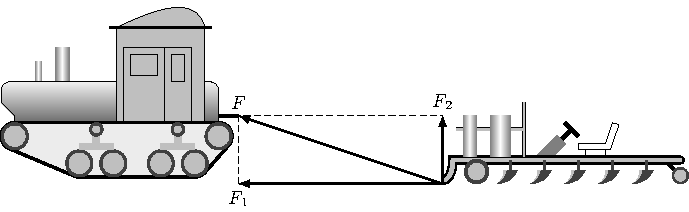
\includegraphics{fig/A/1-27.pdf} 
\caption{} \label{fig_A_1-27} 
\end{figure} 

    因为分力的合力就是原来被分解的那个力,力的分解是
力的合成的逆运算,所以一个力分解为两个力同样遵守平行
四边形法则.把一个已知力作为平行四边形的对角线,那么
与已知力共点的平行四边形的两个邻边就是已知力的两个分
力.在图 \ref{fig_A_1-27} 中,$F_1$和$F_2$是$F$的两个分力.


    我们知道,如果没有其他限制,对于同一条对角线,可以
作出无数个不同的平行四边形(图~\ref{fig_A_1-28})也就是说,同一个
力$F$可以分解为无数对大小、方向不同的分力.那么,一个已
知力究竟该怎样分解呢?

    把一个物体放在斜面上,物体受到竖直向下的重力,但
它并不能竖直下落,而要沿着斜面下滑,同时使斜面受到压
力.这时重力产生两个效果:使物体沿斜面下滑以及使物体
压紧斜面.因此重力$G$应该分解为这样两个力:平行于斜面
使物体下滑的力$F_1$,垂直于斜面使物体压紧斜面的力$F_2$(图~\ref{fig_A_1-29}).


\begin{figure} [htp]
\centering
\begin{minipage} [t]{0.48\textwidth} 
\centering
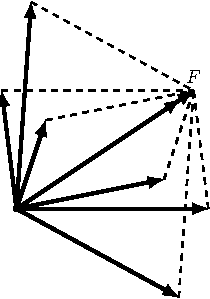
\includegraphics{fig/A/1-28.pdf} 
\caption{} \label{fig_A_1-28} 
\end{minipage} 
\begin{minipage} [t]{0.48\textwidth} 
\centering
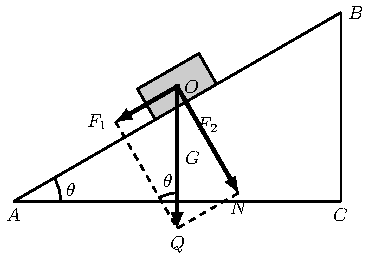
\includegraphics{fig/A/1-29.pdf} 
\caption{} \label{fig_A_1-29} 
\end{minipage} 
\end{figure} 

    如果已知斜面的倾角$\theta$,就可以求出分力$F_1$和$F_2$的大
小.由于直角三角形$ABC$与$OQN$相似,所以
\[\begin{split} 
F_1&= G\sin\theta \\
F_2&= G\cos\theta \\
\end{split}  \]
可以看出,$F_1$和$F_2$的大小都和斜面的倾角有关.斜面的倾
角增大时,$F_1$增大,$F_2$减小.车辆上桥时,力$F_1$阻碍车辆前
进;车辆下桥时,力$F_1$使车辆运动加快.为了行车方便与安
全,高大的桥要造很长的引桥,来减小桥面的坡度.

    把重量为$G$的物体挂在图 \ref{fig_A_1-30} 所示的支架上,物体通过
绳子使支架上的$O$点受到一个向下的作用力$F$,大小等于物
体的重量$G$.力$F$对支架的两个梁产生的效果是什么呢?如
果在$M$和$N$处加上小弹簧,可以看到$M$处的弹簧受到压缩,$N$
处的弹簧受到拉伸.这时力$F$产生两个效果:沿$NO$方向拉
斜梁,沿$OM$方向压横梁.因
此应该把力$F$分解为这样两个
力:沿$NO$方向拉斜梁的力$F_1$,
沿$OM$方向压横梁的力$F_2$.设
斜梁跟墙的夹角为$\theta$,可以看出,
\[\begin{split} 
F_1&= F/\cos\theta \\
F_2&= F\tan\theta \\
\end{split}  \]

\begin{figure} [htp]
\centering
\begin{minipage} [t]{0.48\textwidth} 
\centering
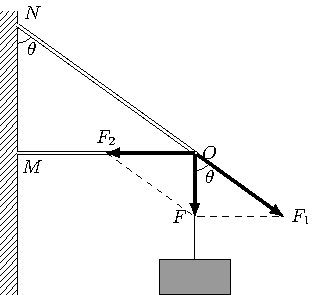
\includegraphics{fig/A/1-30.pdf} 
\caption{} \label{fig_A_1-30} 
\end{minipage} 
\begin{minipage} [t]{0.48\textwidth} 
\centering
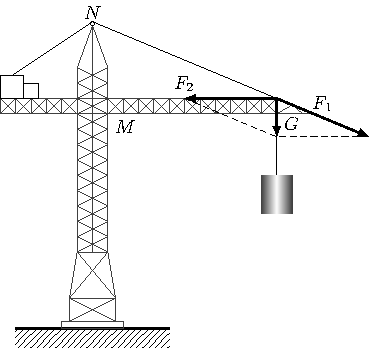
\includegraphics{fig/A/1-31.pdf} 
\caption{} \label{fig_A_1-31} 
\end{minipage} 
\end{figure} 

    从上述例子可以看出,分解一个力要具体考虑这个力产
生的效果,一个力我们可以根据它产生的效果来分解它.


\subsection*{练习七} 
\begin{enumerate} 

\item 一个物体的重量是20牛,把它放在一个斜面上,斜面
长$AB$与斜面高$BC$之比是$5:3$.把重力分解,求出平行于斜面
使物体下滑的力和垂直于斜面使物体压紧斜面的力.
 


\item 图 \ref{fig_A_1-31} 是塔式起重机,钢索$NO$与水平悬臂$MO$成
$30^\circ$角,当起重机吊着$4.0\times 10^4$牛的货物时,钢索和悬臂分别受
多大的力?
\item 如图 \ref{fig_A_1-32} 所示,垂直作用在帆上的风力$F=1.0\times 10^4$
牛.沿着船身方向的分力$F_1$使帆船前进,垂直于船身方向的
分力$F_2$使船身侧倾.设$F$与船身方向成$45^\circ$角,求力$F_1$是多大.
\begin{figure} [htp]
\centering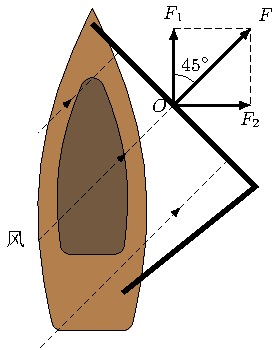
\includegraphics{fig/A/1-32.pdf} 
\caption{} \label{fig_A_1-32} 
\end{figure} 

\item 把竖直向下的180牛的力分解为两个分力,一个分力
在水平方向上并等于240牛,求另一个分力的大小和方向.

\item 一个小同学跟一个大同学拔河,小同学拉不动大同
学,可是用下述办法,小同学就可以拉动大同学.在树干上
拴一条绳子,大同学拿着绳子的另一端,沿水平方向把绳子拉
紧.小同学用力推绳子的中点,就可以拉动大同学了.实际
做一做,并解释所发生的现象.

\end{enumerate} 

\section{矢量和标量} 
    我们在初中学过长度、质量、时间等等物理量.这些物理
量的大小可以用一个带有单位的数值来表示.例如说铅笔长
15厘米,钢块的质量是50千克等等.我们用15厘米就能完
全描述这支铅笔的长度,用50千克就能完全描述这块钢的质
量.力是有大小的,我们也可以用带有单位的数值来表示力.
例如说这个力是10牛,那个力是6牛.可是,这样并没有把
一个力完全表达出来.因为力不但有大小,而且有方向.相
同大小的力,方向不同,它们的作用效果并不相同.要把一个
力完全表达出来,除了说明它的大小,还要指明它的方向才
行.

    这种既有大小又有方向的物理量,除了力而外,在物理学
中还有很多.我们在初中学过的速度也是这类物理量.我们说
一辆汽车的速度是60千米/小时,这并没有把汽车的运动情况完全表达出来,因为这只能说明汽车运动得多快,而没有
说明汽车运动的方向.速度不但有大小,而且有方向.速度
的方向就是物体运动的方向.

    这样,我们就接触到一类物理量.它们的共同特点是:既
有大小,又有方向.这种既有大小又有方向的物理量,叫做\textbf{矢
量} .力是矢量,速度也是矢量.那些只有大小没有方向的物
理量,叫做\textbf{标量} .长度、质量、时间是标量,初中学过的功、温
度等也是标量.

    矢量可以用一根带箭头的线段来表示.线段按一定标度
画出,线段的长短表示矢量的大小,箭头的指向表示矢量的方
向.前面讲的力的图示,其实就是力矢量的表示.速度矢量
以及所有其他矢量都可以这样来表示.

    标量和矢量不仅含义不同,而且服从不同的运算规则.

    两个同类的标量,例如两个质量,只要它们的数值和单位
都相同,比如说都是12千克,我们就说这两个量是相等的.矢
量则不然.两个同类的矢量,它们的大小相等,但方向不同,
就不能说这两个矢量是相等的.比如两个力都是15牛,但方
向不同,就不能说这两个力矢量相等.两个矢量只有大小相
等而且方向相同,才是相等的.

    两个同类的标量,只要单位相同,它们的数值就可以用代
数加法来运算.比如一个质量是10千克,另一个质量是5千
克,总质量就是15千克.矢量则不能这样运算.一个物体受
到两个力,一个是10牛,一个是5牛.这两个力共同作用所
产生的效果不仅决定于它们的大小,而且决定于它们的方向.
前面讲的力的合成就充分说明了这一点.力的合成要按照平
行四边形法则来进行.平行四边形法则不仅适用于力的合
成,对于别的矢量(如速度矢量)同样适用,是矢量合成即矢量
加法运算的普遍法则.

    认识到矢量和标量的不同,这是物理学研究中的一大进
步.有了矢量的概念并且运用矢量的运算规则,我们就能很
方便地研究和处理一些物理问题.

\section{同一直线上的矢量的运算} 
    本书中常常要处理同一直线上的矢量,这一节我们以力
矢量为例讲一讲同一直线上的矢量的运算,以备以后的应用.
这里虽然是以力矢量为例来讲的,但对任何矢量都适用.

    矢量既有大小,又有方向.如果被运算的矢量在一条直
线上,那么,我们就可以用一个带有正负号的数值把矢量的大
小和方向都表示出来.为此,我们沿着矢量所在的直线选定
一个正方向(图~\ref{fig_A_1-33}),规定凡是方向跟正方向相同的矢量都
取正值,凡是方向跟正方向相反的矢量都取负值,例如图中
$F_1=5$牛,$F_2=-5$牛,$F_3=7$牛,$F_4=-5$牛.这里,根据数值
的正负号就可以知道力的方向;而力的大小等于它们的绝对
值,分别是5牛,5牛,7牛,5牛.

\begin{figure} [htp]
\centering
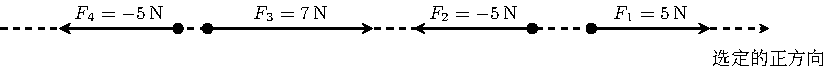
\includegraphics{fig/A/1-33.pdf} 
\caption{} \label{fig_A_1-33} 
\end{figure} 

既然同一条直线上的矢量可以用带正负号的数值来表
示,它们的运算就可以简化为代数运算.

    如果两个矢量大小相等而且方向相同,如图 \ref{fig_A_1-33} 中的
$F_2$和$F_4$,我们就说这两个矢量相等,写成代数式就是
\begin{equation} 
F_2=F_4
\end{equation} 

    如果两个矢量大小相等而方向相反,如图 \ref{fig_A_1-33} 中的$F_1$和$F_2$,
那么,它们只是符号相反,写成代数式就是
\begin{equation} 
F_1=-F_2
\end{equation} 

    如图 \ref{fig_A_1-34} 所示,设有两个力$F_1$和$F_2$作用在一个物体
上,我们可以利用加法运算求出合力$F$:
\begin{equation}\label{eq-A-1.5}
\begin{split} 
F&=F_1+F_2\\
&=10+(-6)=4\text{ 牛} 
\end{split} 
\end{equation} 
这表示合力的大小是4牛,结果是正值表示合力的方向与选
定的正方向相同,即合力的方向跟两个力中较大的那个力的
方向相同.

\begin{figure} [htp]
\centering
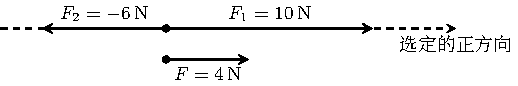
\includegraphics{fig/A/1-34.pdf} 
\caption{} \label{fig_A_1-34} 
\end{figure} 

    我们也可以利用减法运算求分力.如图 \ref{fig_A_1-35} 所示,已知
合力$F$和一个分力$F_1$,那么,另一个分力$F_2$:
\begin{equation} 
\begin{split} 
F_2&=F-F_1\\
&=8-(-3)=11\text{ 牛} 
\end{split} 
\end{equation} 
这表示$F_2$的大小是11牛,方向与选定的正方向相同.

需要强调指出的是:\textit{只有同一直线上的矢量,它们的运
算才可以像上述那样简化成代数运算.这是平行四边形法则
在这种特殊情况下的运用} .不在同一直线上的矢量,它们的运算不能
这样简化成代数运算,仍必须按照平行四边形法则
来进行.

\begin{figure} [htp]
\centering
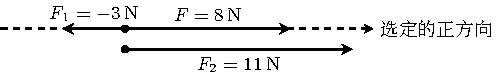
\includegraphics{fig/A/1-35.pdf} 
\caption{} \label{fig_A_1-35} 
\end{figure} 

    还要指出的是:这里用带有正负号的数值既表示出矢量
的大小,又表示出矢量的方向;如果专指矢量的大小,就要取
绝对值,即矢量的大小总是正值.本章前面各节中的公式,如
公式
\[\begin{split} 
f&=kx\\
f&=\mu N\\
F&=\sqrt{F^2_1+F^2_2+2F_1F_2\cos\theta} \\
F&=F_1+F_2\quad (\theta =0^\circ)\\
F&=F_1-F_2\quad (\theta =180^\circ)\\
\end{split}  \]
等等都是关于力矢量大小的公式.利用这些公式来计算.其
中的各力都取正值.例如用$F=F_1-F_2$来计算图 \ref{fig_A_1-34} 中的
合力时,$F_1=10$牛,$F_2=6$牛,$F=F_1-F_2=4$牛.这与 \ref{eq-A-1.5} 式
所得结果相同.初学时概念上要弄清楚,熟悉起来以后,就可
以根据物理思考灵活运用了.


\subsection*{复习题} 

\begin{enumerate} 
\item 从力的性质看,力学中经常遇到的有哪几种力?这几
种力的情况是怎样的?力可以用哪两种方法来分类?为什么说
拉力、压力和支持力都是弹力?
\item
胡克定律的内容是什么?写出胡克定律的公式.
\item
怎样计算滑动摩擦力的大小?写出它的公式.
\item 牛顿第三定律的内容是什么,为什么说作用力和反
作用力不能互相平衡?
\item
力的合成要按照什么法则来进行?这个法则的内容
又什么,写出计算合力的大小和方向的公式.
\item
为什么力的分解和合成遵守相同的法则?一个力可
以根据什么来分解它?一个力,如果知道它的两个分力的方
向,或者知道它的一个分力的大小和方向,那么,这个力的分
解有没有确定的答案?
\item
什么叫矢量?什么叫标量?矢量和标量有什么不同?
矢量加法要按照什么法则来运算?
\item
你自己总结一下应该怎样分析物体的受力情况,分
析时应该注意什么?
\end{enumerate} 

\section*{习题} 

\begin{enumerate} 
\item   如图 \ref{fig_A_1-36} 所示,为了防止电线杆倾倒,常在两侧对称
地拉上钢绳.如果两条钢绳间的夹角是$60^\circ$,每条钢绳的拉力
都是300牛,求两条钢绳作用在电线杆上的合力.

\begin{figure} [htp]
\centering
\begin{minipage} [t]{0.48\textwidth} 
\centering
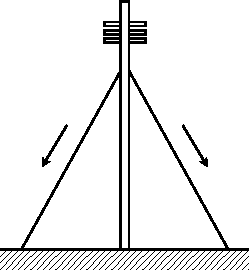
\includegraphics{fig/A/1-36.pdf} 
\caption{} \label{fig_A_1-36} 
\end{minipage} 
\begin{minipage} [t]{0.48\textwidth} 
\centering
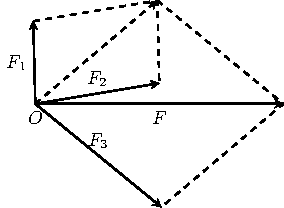
\includegraphics{fig/A/1-37.pdf} 
\caption{} \label{fig_A_1-37} 
\end{minipage} 
\end{figure} 


\item  图 \ref{fig_A_1-37} 表示用平行四边形法则求三个共点力$F_1$、$F_2$、$F_3$
的合力$F$.先求出$F_1$和$F_2$的合力,再求出这个合力与$F_3$的
合力$F$.改用三角形法求出这三个力的合力.改变求和的顺
序,再分别用平行四边形法则和三角形法求出这三个力的合
力.



\item   20牛、30牛和40牛的三个力作用于物体的一点,它们
之间的夹角都是$120^\circ$.求合力的大小和方向.

\item 如图 \ref{fig_A_1-38} 所示,把一个重量为10牛的物体挂在绳子
上,已知$AC=BC=3$米,$CD=1$米.求绳$AC$和$BC$所受的拉
力.
\begin{figure} [htp]
\centering
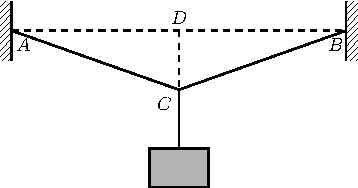
\includegraphics{fig/A/1-38.pdf}
\caption{} \label{fig_A_1-38} 
\end{figure} 


\item   用手握着橡皮绳的两端,在橡皮绳的中间挂一个重
物,当两手之间的距离增大或减小的时候,物体对橡皮绳的
拉力是否改变?怎样改变?实际做一下,并说明道理.

\item  刀、斧、凿、刨等切削工具的刃部叫做劈,劈的纵截面
是一个三角形,如图~\ref{fig_A_1-39} 所示.使用劈的时候,在劈背上加力
$F$,这个力产生两个效果,这就是使劈的两个侧面推压物体,
把物体劈开.设劈的纵截面是一个等腰三角形,劈背的宽度
是$d$,劈的侧面的长度是$\ell$,可以证明:
\[f_1=f_2=\frac{\ell} {d} F \]

从上式可知,当$F$一定的时侯,劈的两个侧面之间的夹角
越小,$\ell/d$就越大,$f_1$和$f_2$就越大.这说明了为什么越锋利的
切削工具越容易劈开物体.试证明上式.



\item 一个物体放在倾角为$\theta$的光滑斜面上,求物体受到
的合力.
\begin{figure} [htp]\centering
\begin{minipage} [t]{0.48\textwidth} 
\centering
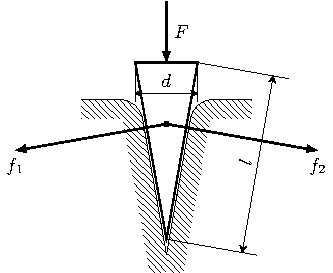
\includegraphics{fig/A/1-39.pdf} 
\caption{} \label{fig_A_1-39} 
\end{minipage} 
\begin{minipage} [t]{0.48\textwidth} 
\centering
\includegraphics{fig/A/1-40.pdf} 
\caption{} \label{fig_A_1-40} 
\end{minipage} 
\end{figure} 

\begin{solution} 
放在斜面上的物体受到两个力的作用:重力$G$和斜
面的支持力$N$(图~\ref{fig_A_1-40}),现在已知$N$的方向,但不知道$N$的
大小.我们把重力$G$分解为两个分力:平行于斜面的分力
$F_1=G\sin\theta$,垂直于斜面的分力$F_2=G\cos\theta$.这样,物体相当
于受到$G\sin\theta$、$G\cos\theta$和$N$这三个力的作用.因为物体沿着斜
面运动,在垂直于斜面的方向上不发生运动,所以垂直于斜面
方向的两个力$N$和$G\cos\theta$是互相平衡的,它们大小相等,即
$N=G\cos\theta$.因此,物体受到的合力的大小为$G\sin\theta$,方向平行
于斜面向下.


 \hskip 2em    这里我们先把一个力分解,然后求出合力.这种方法以
后我们还会用到.

 \hskip 2em    我们看到,放在光滑斜面上的物体,所受的合力实际上等
于重力的一个分力$G\sin\theta$,在这个力的作用下物体将沿着斜
面下滑,但是,如果斜面不是光滑的,或者物体还受到别的力,
合力将不再等于重力的一个分力$G\sin\theta$.
\end{solution} 
   

\item 一个滑雪人沿着山坡滑下.滑雪人的重量是700牛,
山坡的倾角是$30^\circ$,滑雪板和雪地的滑动摩擦系数是0.04.求
滑雪人所受的合力.

\end{enumerate} 


















 %力
	%\chapter{直线运动}\label{chapter-rectilinear-motion}

\section{机械运动}
 我们在初中学过,一个物体相对于另一个物体的位置变
化叫做\NoteBold{机械运动},简称运动.在自然界中没有不动的物体.房
屋、桥梁、树木、山岭等总在原地不动,我们说它们是静止的.
其实它们是随着地球一起运动的,不但地球在运动,太阳在
银河系中也是运动的.小到原子和分子,大到宇宙中的天体,
一切物体都在运动.
机械运动是宇宙中最普遍的现象.

\subsection{参照物} 

既然一切物体都在运动,我们研究一个物体的
运动时,就必须选取另外的物体作为参照,事先假定这个另外
的物体是不动的,这样才能进行研究.我们说房屋、桥梁等是
静止的,行驶的汽车是运动的,这是选取地面作为参照来说
的;房屋、桥梁等对地面来说位置没有发生变化,行驶的汽车
对地面来说位置发生了变化.坐在行驶的火车车厢里的乘客
认为自己是静止的,在车厢里走动的乘务员是运动的,这是
选取车厢作为参照来说的;乘客对车厢来说位置没有发生变
化,乘务员对车厢来说位置发生了变化.研究物体的运动时,
选来作为参照的另外的物体,叫做\NoteBold{参照物}.

    原则上,研究一个物体的运动时,参照物是可以任意选取
的.观察在河里游泳的人的运动,可以选择河岸作参照物,也
可以选择在河上航行的船只作参照物.研究天体的运动时,可
以取地球作参照物,也可以取太阳作参照物.但是,实际选取
参照物时,往往要考虑研究问题的方便,使运动的描述尽可能
简单.例如,研究太阳系的行星运动,太阳是最理想的参照物.
研究地面上物体的运动,一般说来取地面做参照物比较方便.

\subsection{平动和转动} 
 物体的运动一般是比较复杂的,但是最基
本的运动只有两种:平动和转动.

    从桌内拉出抽屉的时候,抽屉各部分的运动轨迹完全相
同,也就是说,各部分的运动完全相同.这样的运动就是\NoteBold{平
动}.打桩时重锤的下落运动,汽缸里活塞的运动,车床上车刀
(图~\ref{fig_A_2-1})的运动,在直铁轨上行驶的火车车厢的运动,都是平
动.
\begin{figure}[htbp]
    \centering
    \includegraphics{fig/A/2-1.pdf}
    \caption{车床上车刀的平动和工件的转动}\label{fig_A_2-1}
\end{figure}

    物体的平动不一定都沿着直线进行,也可以沿曲线进行,
图~\ref{fig_A_2-2} 所示的铅笔的平动就是沿着曲线进行的.
\begin{figure}[htbp]
    \centering
    \begin{minipage}[t]{0.48\textwidth}
        \centering
        \includegraphics{fig/A/2-2.pdf}
        \caption{沿曲线进行的平动}\label{fig_A_2-2}
    \end{minipage}
    \begin{minipage}[t]{0.48\textwidth}
        \centering
        \includegraphics{fig/A/2-3.pdf}
        \caption{钻头在工作中同时做平动和转动}\label{fig_A_2-3}
    \end{minipage}
\end{figure}
    
    推动石磨的时候,磨盘上的各部分都围绕着通过中心
的轴线做圆周运动.这样的运动就是\NoteBold{转动}.脱粒机的滚筒的
运动,机器上飞轮的运动,车床上工件的运动(图~\ref{fig_A_2-1}),都是
转动.


    在很多情况下,物体同时做平动和转动.钻头在工作的
时候(图~\ref{fig_A_2-3}),车轮在路上滚动的时候,螺栓在拧入螺母中的
时候,都是同时做平动和转动的.

\section{质点}
    物体都具有大小和形状,在运动中物体各点的位置变
化一般说来是各不相同的,所以要详细描述物体的运动,并不
是一件简单的事情.可是,在某些倩况下,却可以不考虑物体
的大小和形状,而使问题简化.在这些情形下,我们可以把物
体看作一个有质量的点,或者说用一个有质量的点来代替整
个物体,用来代替物体的有质量的点叫做\NoteBold{质点}.

    在什么情况下可以把物体当作质点,这要看具体情况而
定.举例来说,当我们研究地球的公转时,由于地球的直径(约
$1.3\times 10^4$千米)比地球和太阳之间的距离(约$1.5\times 10^8$千米)
要小得多,因而可以忽略地球的大小和形状,把它当作质点.
可是研究地球的自转时,我们却不能忽略地球的大小和形状,
当然不能把地球当作质点了.

    一个平动的物体,它的各个部分的运动情况都相同,它的
任何一点的运动都可以代表整个物体的运动.在这种情况
下,也可以把整个物体当作质点来看待.一辆在直公路上行
驶的汽车,车身上各部分的运动情况相同,当我们把汽车作为
一个整体来研究它的运动的时侯,就可以把汽车当作质点.当
然,假如我们需要研究汽车的轮胎的运动,由于轮胎的各部分
的运动情况不相同,那就不能把它看作质点了.

    今后我们研究的物体,除非涉及到转动,一般都可以看作
质点.

    任何物体都具有一定的大小和形状,因此质点这个概念
是一种科学的抽象,是一种理想化的模型.我们研究物体的
运动,像研究其他物理现象一样,不能主次不分.如果物体的
大小和形状在所研究的现象中起的作用很小,可以忽略不计,
我们就可以把物体看作是一个没有大小和形状的理想物体,
即质点.这种研究问题的方法,在物理学中是常常用到的.

    研究物体的运动,第一步是要知道物体是怎样运动的,也
就是知道物体的运动情况.物体在运动过程中,它的位置和
速度不断随时间而变化,如果我们知道了物体在任一时刻的
位置和速度,就表示我们知道了物体的运动情况.这一章我
们就围绕着这个要求来研究直线运动.

 \subsection*{练习一}
\begin{enumerate}
\item 两辆在公路上直线行驶的汽车,它们的距离保持不
变.试说明用什么样的物体做参照物,两辆汽车都是静止的,
用什么样的物体做参照物,两辆汽车都是运动的.能否找到
这样一个参照物,一辆汽车对它是静止的,另一辆汽车对它是
运动的?为什么?

\item 小孩从滑梯上滑下,钢球沿斜槽滚下,石块从手中
落下,这些物体中哪些是做平动的?

\item 研究自行车轮的转动,能不能把自行车当作质点?研
究在马路上行驶的自行车的速度,能不能把自行车当作质点?
\end{enumerate}

\section{位置和位移}
    研究质点的运动,首先要知道怎样确定质点的位置.质
点的位置可以采取在数学中学过的建立坐标系的方法来确
定.质点做直线运动时,我们可以取这条直线为坐标轴($x$
轴),在轴上任选一点$O$为原点,规定好坐标轴的正方向和单
位,质点的位置由它的位置坐标,即一个带有正负号的数值,
就可以完全确定了.比如我们要确定一辆行驶在北京长安街
上的汽车的位置,我们可以取$x$轴表示长安街的东西方向,$x$
轴的正方向指东,并且取天安门前的旗杆作为坐标原点,那么
汽车的位置就由它的坐标完全确定了.汽车的坐标是1千
米,表示它在旗杆以东1千米处;汽车的坐标是$-2$千米,表
示它在旗杆以西2千米处(图~\ref{fig_A_2-4}).
\begin{figure}[htbp]
    \centering
    \includegraphics{fig/A/2-4.pdf}
    \caption{}\label{fig_A_2-4}
\end{figure}

    质点在运动过程中,它的位置随时间不断变化,怎样表
示质点的位置变化呢?物理学中用一个叫做位移的物理量来
表示质点位置的变化.设质点原来在$A$点,经过一段时间沿
轨迹$ACB$运动到$B$点(图~\ref{fig_A_2-5}).从初位置$A$指向末位置$B$
作线段$AB$,用它就可以描述质点的位置变化,我们把它叫做
质点的位移.$AB$的长度,即位移的大小,表示出位置变化的
大小;$AB$的方向,即位移的方向,表示出位置变化的方向.位
移既有大小,又有方向,是一个矢量.

\begin{figure}[htbp]
    \centering
    \includegraphics{fig/A/2-5.pdf}
    \caption{}\label{fig_A_2-5}
\end{figure}


    位移和路程是两个不同的物理量.路程是指质点所通过
的实际轨迹的长度,只有大小,没有方向,是标量.在图~\ref{fig_A_2-5} 
中,质点的位移是线段$AB$,而路程是曲线弧$\wideparen{ACB}$的长度,即
使在直线运动中位移的大小也不一定等于路程.图~\ref{fig_A_2-6} 表示
做直线运动的质点从初位置$A$经过$B$运动到$C$,然后从$C$返
回,运动到末位置$B$,这时质点的位移是线段$AB$,而路程是
线段$AC$的长度加上线段$BC$的长度.只有做直线运动的质
点始终向着同一个方向运动时,位移的大小才等于路程.可
见,位移矢量一般并不表示运动的实际轨迹和路程,而是表示
位置的变化.
\begin{figure}[htbp]
	\centering
	\includegraphics{fig/A/2-6.pdf}
	\caption{}\label{fig_A_2-6}
\end{figure}


    在物理学中,通常用$s$代表位移.质点做直线运动时,位
移可以用末位置的坐标$x$和初位置的坐标$x_0$表示出来:
\[s=x-x_0\]
\begin{figure}[htbp]
    \centering
    \begin{subfigure} {1\linewidth} 
        \centering
        \includegraphics{fig/A/2-7a.pdf} 
        \caption{}\label{fig_A_2-7a} 
    \end{subfigure} 
    \\
    \begin{subfigure} {1\linewidth} 
        \centering
        \includegraphics{fig/A/2-7b.pdf} 
        \caption{}\label{fig_A_2-7b} 
    \end{subfigure} 
    \caption{位移的坐标表示}\label{fig_A_2-7}
\end{figure}

这就是说,位移的数值等于末位置的坐标$x$减去初位置
的坐标$x_0$.在图~\ref{fig_A_2-7} 中,$A$点表示初位置,$B$点表示未位置.图~\ref{fig_A_2-7a}
中,$s=x-x_0=4-2 \Um =2 \Um $,位移是正值,它的大小
是2米,方向与坐标轴的正方向相同.图~\ref{fig_A_2-7b} 中,$s=x-x_0=-5-1 \Um =-6 \Um $,位移是负值,它的大小是6米,方向与
坐标轴的正方向相反.可见,在直线运动中,用一个带有正
负号的数值就可以把位移矢量的大小和方向都表示出来.

    为了方便,在计算位移时常常取初位置为坐标原点,即
$x_0=0$.这时质点的位移就可以用末位置的坐标来表示:
\[s=x\]

\subsection*{练习二}
\begin{enumerate}
  \item   质点做什么运动,位移的大小才等于路程?
  \item  图~\ref{fig_A_2-6} 表示做直线运动的质点从初位置$A$经过$B$运
  动到$C$,然后从$C$返回,运动到末位置$B$.设$AB$长7米,$BC$长
  5米.求质点的位移的大小和路程.
  \item 在图~\ref{fig_A_2-4} 中,汽车初位置的坐标是$-2$千米,末位置的
  坐标是1千米.求汽车的位移的大小和方向.
  
\end{enumerate}


\section{匀速直线运动~~速度}
    现在我们开始研究物体的运动.从哪里来开始呢?也许从
最常见的运动开始比较好吧!一片树叶从树枝上落下是一种
很常见的运动,可是仔细观察一下,却发现这种运动很复杂,
树叶忽左忽右,有时还发生翻转等,不便于研究.物理学中
研究问题常常是从最简单的现象着手.因此,我们从最简单
的运动即匀速直线运动来开始对运动的研究.

    火车在平直的铁路上行驶,如果它每分钟的位移是900
米,每秒钟的位移是15米,也就是在相等的时间内位移相等,
这列火车所做的运动就是\NoteBold{匀速直线运动}.

\NoteUnderWave{物体在一条直线上运动,如果在相等时间里的位移相等,
这种运动就叫做匀速直线运动}.匀速直线运动有时简称为\NoteBold{匀速运动}.

    飞机在天空中匀速飞行,轮船在海洋上匀速航行,它们的
运动虽然都是匀速运动,但还是有区别的.在相同的时间里,
飞机的位移大,轮船的位移小,即飞机飞得快,轮船走得慢.在
物理学中怎样来表示匀速运动的快慢呢?在匀速运动中,物
体在相等时间内的位移相等,因此,如果物体在时间$t$内的位
移是$s$,在$2t$时间内的位移一定是$2s$,在$3t$时间内的位移
一定是$3s$,等等.可见匀速运动的位移和时间的比值是一个
恒量,不随时间而改变.这个比值越大,表示物体运动得越
快.

\NoteUnderWave{在匀速直线运动中,位移和时间的比值,叫做匀速直线
运动的\NoteBold{速度}}.

如果做匀速运动的物体在时间$t$内的位移是$s$,速度$v$
就可以用下式来表示:
\[v=\frac{s}{t} \]

由上式可以看出,速度在数值上等于单位时间内位移的
大小.

    速度的单位有厘米/秒,米/秒,千米/小时等.在国际单
位制中,速度用米/秒($\UmsA$)作单位.

    速度不但有大小,而且有方向,是矢量.速度矢量的方向
就是物体位移的方向.在匀速直线运动中,计算时通常取位
移方向作为正方向,速度是正值.

从速度的公式$v=s/t$
可以得到
  \[s=vt \]

这个公式叫做匀速运动的\NoteBold{位移公式},它表示出匀速运动
的位移跟时间的关系:位移跟时间成正比.利用这个公式,只
要知道了速度$v$,就可以求出做匀速运动的物体在任何时间
内的位移.如果还知道物体的初位置,就可以确定做匀速运
动的物体在任一时刻所在的位置.

这里提到了时间和时刻,顺便说一下它们的区别.我们说.
现在是9时10分,这是指的时刻.我们说从9时10分到9
时50分,这是指的一段时间,这段时间是40分钟.如果用坐
标轴来表示时间,那么时刻相当于轴上的一点,时间相当于轴
上的一段距离.坐标轴原点的时刻为零,$t=0$,表示从这一时
刻开始计时.

\subsection*{练习三}

\begin{enumerate}
    \item 光在真空中沿直线传播的速度为$3.0\times 10^8\Ums$.
\begin{enumerate}
    \item 一光年(光在一年中传播的距离)有多少千米?
    \item 最靠近我们的恒星(半人马座$\alpha$星)离我们$4.0\times 10^{13}$千米,它发出的光要多长时间才到达地球?
\end{enumerate}    
\item  在技术上常用$\UkmhA$作速度的单位.试求$1 \Ums$合多少$\UkmhA$.
\item 光在空气中的速度可以认为等于光在真空中的速
度.声音在空气中的速度是340$\Ums$.一个人看到闪电后5
秒听到雷声,打雷的地方离他大约多远?

\end{enumerate}

\section{匀速直线运动的图像}
    物体运动的情况可以用公式来表示,也可以用函数图像
来表示.这一节学习怎样用图像来表示匀速直线运动.

    \subsection{匀速直线运动的位移图像} 
    
    任意选择一个平面直角坐标
系,用横轴表示时间,用纵轴表示位移,画出位移和时间的关
系图线,这种图像叫做\NoteBold{位移—时间图像},简称为\NoteBold{位移图像}.
匀速直线运动的位移$s$
是时间$t$的正比函数$s=vt$.


在初中数学里已经学过,正比函数的图像是一条通过原
点的直线.图~\ref{fig_A_2-8} 中的直线~I是速度为$2 \Ums$的匀速运动
的位移图像,直线II是速度为$v=3 \Ums$的位移图像.
\begin{figure}[htbp]
	\centering
	\includegraphics{fig/A/2-8.pdf}
	\caption{匀速运动的位移图像.
		取初位置为坐标原点时,质点的位移等于末位置的坐标,因此这个
		图像也可以叫做质点的位置—时间图像.}\label{fig_A_2-8}
\end{figure}



    应用匀速运动的位移图像,我们可以求出物体在任意时
间内的位移.例如从图~\ref{fig_A_2-8} 可以求出,$v=2\Ums$的匀速运动
在2.5秒内的位移是5米.
应用位移图像也可以反过来求出
物体通过任一位移所需的时间.


我们还可以从匀速运动的位移图像求出物体的速度.

\begin{figure}[htbp]
    \centering
    \includegraphics{fig/A/2-9.pdf}
    \caption{匀速运动的速度等
    于位移图线的斜率}\label{fig_A_2-9}
\end{figure}

在图~\ref{fig_A_2-9} 所示的匀速运动的位移图线$OP$上,任取两点
$P_1(t_1,s_1)$和$P_2(t_2,s_2)$.用$\Delta t$表示$t_2-t_1$,用$\Delta s$
表示$s_2-s_1$.
在直角三角形$P_1QP_2$中,比值
$\dfrac{\Delta s}{\Delta t}=\dfrac{QP_2}{P_1Q}$越大,
$\angle P_2P_1Q$也越大,直线$OP$就越陡.所以我们把
$\Delta s/\Delta t$叫做直线的\NoteBold{斜
率},用字母$k$来表示.$\Delta s$是物体在$\Delta t$内的位移,比
值 $\Delta s/\Delta t$
是匀速运动的速度$v$,因此
\[k=\frac{\Delta s}{\Delta t}=v\]

这样,我们得到结论:在匀速直线运动中,位移图线的斜
率等于运动的速度.在同一个坐标平面上,斜率越大,即直线
越陡,表示速度越大.

 
\subsection{匀速直线运动的速度图像} 

匀速直线运动的速度和时间
的关系,也可以用图像来表示.

在平面直角坐标系中,用横轴表示时间,用纵轴表示速
度,画出速度和时间关系的图线,这种图像叫做运动的\NoteBold{速度—时间图像},简称为\NoteBold{速度图像}.匀速运动的速度不随时间改变,
它的速度图像是一条与横轴平行的直线,图~\ref{fig_A_2-10} 中的两条直
线I和II分别表示$v=2$$\Ums$和$v=5$$\Ums$的匀速运动的
速度图像.在同一个坐标平面上,图像的直线在纵轴上的截
距越大,表示速度越大.
\begin{figure}[htbp]
    \centering
    \begin{minipage}[t]{0.48\textwidth}
        \centering
        \includegraphics{fig/A/2-10.pdf}
        \caption{匀速运动的速度图像}\label{fig_A_2-10}
    \end{minipage}
    \begin{minipage}[t]{0.48\textwidth}
        \centering
        \includegraphics{fig/A/2-11.pdf}
        \caption{由速度图像求位移}\label{fig_A_2-11}
    \end{minipage}
\end{figure}

应用速度图像可以求出质点在任何时间内的位移.
设有一个骑自行车的人以3$\Ums$的速度做匀速运动,速度图像如
图~\ref{fig_A_2-11} 所示.现在来求他在5秒钟内的位移.为了求出位
移,根据公式$s=vt$,必须用时间和速度相乘,也就是用横轴
上的线段$OA=5$秒和纵轴上的线段$OB=3$$\Ums$相乘.图~\ref{fig_A_2-11} 
中画有斜线的长方形的“面积”,表示的就是这个位移的
大小,它的数值是$3 \Ums \times 5 \Us = 15 \Um$,也就是说,位移的数
值等于这个长方形“面积”的数值.这里我们把“面积”一词打
上引号,是因为这个长方形的底的单位是$\UsA$,高的单位是$\UmsA$,这个面积的单位是$\UmsA \times \UsA= \UmA $,而不是$ \UmqA $.

\subsection*{练习四}
\begin{figure}[htbp]
    \centering
    \begin{minipage}[t]{0.48\textwidth}
        \centering
        \includegraphics{fig/A/2-12.pdf}
        \caption{}\label{fig_A_2-12}
    \end{minipage}
    \begin{minipage}[t]{0.48\textwidth}
        \centering
        \includegraphics{fig/A/2-13.pdf}
        \caption{}\label{fig_A_2-13}
    \end{minipage}
\end{figure}

\begin{enumerate}
\item 
图~\ref{fig_A_2-12} 是一架民航飞机的位移图像.从这个图像求出
\begin{enumerate}
    \item 飞机在30分钟内的位移;
    \item 飞行700千米所用的时间;
    \item 飞行速度并画出速度图像.
\end{enumerate}

\item  
图~\ref{fig_A_2-13} 是一辆火车运动的位移图像.线段$OA$和$BC$
所表示的运动,哪个速度大?各等于多大?线段AB与横轴平
行,表示火车做什么运动?速度是多大?火车在3小时内的位移
是多少?通过80千米用多长时间?画出火车的速度图像.


\item  
有两个物体,从同一点开始向相同方向做匀速运动,
速度分别是3$\Ums$和5$\Ums$,在同一个坐标平面上画出它们
的位移图像和速度图像,并根据这两种图像分别求出它们在5
秒内的位移.

\end{enumerate}


\section{变速直线运动~~平均速度~~瞬时速度}
    \subsection{变速直线运动}
    
    我们日常看到的直线运动,往往不是匀
速的.飞机起飞的时候,运动越来越快,在相等时间里的位移
是不相等的.火车进站的时候,运动越来越慢,在相等时间里
的位移也是不相等的.

\NoteUnderWave{物体在一条直线上运动,如果在相等时间里的位移不相等,这种运动就叫做\NoteBold{变速直线运动}}.变速直线运动有时简称为\NoteBold{变速运动}.

\subsection{平均速度}

变速运动的物体在相等的时间里的位移不
相等,所以它没有恒定的速度.那么,我们怎样来描述它的快
慢呢?粗略的办法是把它看作匀速运动.一列火车,半小时
内走了28千米,尽管它的运动时快时慢,我们仍然可以设想
火车在这半小时内是匀速运动的,这样它的速度就是$56 \Ukmh$.这个$56 \Ukmh$,就是火车在这半个小时内的\NoteBold{平
均速度}.

\NoteUnderWave{在变速直线运动中,运动物体的位移和所用时间的比值,
叫做这段时间里的平均速度}.
如果用$\bar v$来表示平均速度,那么
\[\bar v=\frac{s}{t}\]

平均速度的数值跟在哪一段时间内计算平均速度有关.
上面讲的那列火车,如果在第一个十分钟走了8千米,在第二
个十分钟走了9千米,在第三个十分钟里走了11千米,它在
三个十分钟里的平均速度就分别是48$\Ukmh$,54$\Ukmh$,66$\Ukmh$.可见,火车半小时内的平均速度虽然是
56$\Ukmh$,但在每个十分钟里的平均速度却是不同的,它
的运动逐步加快.

\subsection{瞬时速度}
平均速度只能粗略地描述做变速运动的物体
的运动情况,要精确地描述变速直线运动,还需要知道物体在
每一时刻(或位置)的运动速度.运动物体在某一时刻(或某
一位置)的速度,叫做\NoteBold{瞬时速度}.

物体在某一时刻或某一位置的速度的意义是什么呢?图~\ref{fig_A_2-14} 
表示一辆做变速运动的汽车,我们要确定汽车经过$A$点
时的瞬时速度.从$A$起取一小段位移$AA_1$,求出在这段位移上
的平均速度,这个平均速度可以近似地表示汽车经过$A$点的
快慢程度.从$A$起所取的位移越小,比如依次取位移$AA_2$、$AA_3$
等,所得的平均速度用来表示汽车经过$A$点的快慢程度就
越精确.当位移足够小时,
或者说时间足够短时,所得
的平均速度就等于汽车经过$A$点的瞬时速度了.
\begin{figure}[htbp]
	\centering
	\includegraphics{fig/A/2-14.pdf}
	\caption{}\label{fig_A_2-14}
\end{figure}


这里所说的“足够短”,应该怎样理解呢?原来,做变速运
动的物体的速度总是连续变化的,位移取得越小,或者说时间
取得越短,在这段时间内速度的变化就越小.时间足够短时,
测量仪器已经分辨不出变速运动和匀速运动的差别,可以认
为这一小段时间的运动是匀速的.这时,即使进一步缩短所
取的时间,测得的平均速度也不会有什么变化,这个平均速度
就等于瞬时速度.



用数学语言可以更为精确地表达上面所讲的意思.在图~\ref{fig_A_2-14} 
中从$A$起取一小段位移$\Delta s$,求出这小段位移内的平均
速度$\Delta s/\Delta t$, 当$\Delta t$\NoteBold{趋近于}零时,平均速度\NoteBold{趋近于}某一固定数
值——极限值,这个极限值就是汽车经过$A$点的瞬时速度.

    瞬时速度既有大小,又有方向,是矢量.在直线运动中,
瞬时速度的方向就是物体经过该点时的运动方向.瞬时速度
的大小叫做\NoteBold{瞬时速率},简称\NoteBold{速率},它是一个表示物体运动快慢
程度的标量,在某些问题中,如果只需考虑瞬时速度的大小,
可以用速率的概念.

    在匀速运动中,知道了速度,根据位移公式就可以确定运
动物体在任一时刻的位置,在变速运动中,怎样确定物体在
任一时刻的位置和速度呢?

    一般地讨论这个问题过于复杂,下面我们只就最简单的
变速运动来研究这个问题.

\subsection*{练习五}

\begin{enumerate}
    \item 一辆汽车,起初以30$\Ukmh$的速度匀速行驶了30千米,然后又以60$\Ukmh$的速度匀速行驶了30千米.一位
    同学认为这辆汽车在这60千米中的平均速度是$1/2\cdot(30 \Ukmh+60\Ukmh)=45\Ukmh$.这个结果对不对?
    \item 骑自行车的人沿着坡路下行,在第1秒内通过1米,
    第2秒内通过3米,在第3秒内通过5米,在第4秒内通过7米.求
    最初两秒内、最后两秒内以及全部运动时间内的平均速度.
    \item 在一个速度是$v$的匀速直线运动中,各段时间内的
    平均速度以及整个运动的平均速度各是多大?每一时刻的即
    时速度是多大?
    \item 火车以70$\Ukmh$的速度经过某一路标,子弹以
    600$\Ums$的速度从枪筒射出.这里指的是什么速度?
    
\end{enumerate}


\section{匀变速直线运动~~加速度}
    \subsection{匀变速直线运动}
    
    伽利略($1564 \sim 1642$)是首先认真研究
变速运动的物理学家.伽利略就是从最简单的变速运动着手
的.他设想,最简单的变速运动的速度应该是均匀变化的.
但是,速度的变化怎样才算均匀呢?他考虑了两种可能:一种
是速度的变化对时间来说是均匀的,即经过相等的时间,速度
的变化相等;另一种是速度的变化对路程来说是均匀的,即
经过相等的路程,速度的变化相等.伽利略断定第一种方式最
为简单,并且用实验研究了斜面上滚下来的铜球,证明这种运
动方式在自然界中是的确存在的.这种运动,就是我们现在
要研究的匀变速直线运动.

\NoteUnderWave{在一条直线上运动的物体,如果在相等的时间里速度的
变化相等,
物体的运动就叫做\NoteBold{匀变速直线运动}},或者简称为\NoteBold{匀变速运动}.

举例来说,一个做直线运动的物体,在某一时刻它的速度
是3$\Ums$,过了1秒钟变成4$\Ums$,再过1秒钟变成5$\Ums$,
它的速度每秒钟增加1$\Ums$,这个物体做的就是匀变速运
动.又如一个做直线运动的物体,在某一时刻它的速度是
8$\Ums$,过了1秒钟变成6$\Ums$,再过1秒钟变成4$\Ums$,
它的速度每秒钟减小2$\Ums$,这个物体做的也是匀变速运
动.

    常见的许多变速运动实际上并不是匀变速运劝,可是不
少变速运动很接近于匀变速运动,可以当作匀变速运动来处
理.石块从不高的地方下落的运动,发炮时炮弹在炮筒里的运
动,火车、汽车等交通工具开动后一段时间内的运动,竖直抛
出的石块向上的运动,交通工具在停止前的一段运动,都可以
看作是匀变速运动.

\subsection{加速度}
不同的匀变速运动,瞬时速度的变化有快有慢,
汽车开动时,它的速度在几秒钟内从零增加到几十米每秒.而
发炮时,炮弹的速度在千分之几秒内就从零增加到几百米每
秒.显然汽车的速度增加得慢,炮弹的速度增加得快.火车
进站时速度减小得慢,而汽车在急刹车时速度减小得快.怎样
来表示速度变化的快慢呢?为此,物理学中引入了一个新的
物理量——加速度.

在匀变速直线运动中,在相等的时间里速度的变化相等,
时间$t$增加几倍,速度的变化$v_t-v_0$也增加几倍,因而速度
的变化跟发生这个变化所用的时间的比值是一个恒量,不随
时间而改变.这个比值越大,表示速度变化得越快.

\NoteUnderWave{在匀变速直线运动中,速度的变化和所用的时间的比值,
叫做匀变速直线运动的加速度}.

用$v_0$表示运动物体开始时刻的速度(初速度),用$v_t$表
示经过一段时间$t$的速度(末速度),用$a$表示加速度,那么,
\[a=\frac{v_t-v_0}{t}\]

由上式可以看出,加速度在数值上等于单位时间内速度
的变化.

    加速度的单位是由时间的单位和速度的单位确定的.在
国际单位制中,时间的单位是秒,速度的单位如果用$\UmsA$、加
速度的单位就是$\UmsqA$,读作米每二次方秒.速度的单位如
果用$\UcmsA$,加速度的单位就是$\UcmsqA$.

    加速度不但有大小,而且有方向,因此是矢量.在直线运
动中,取开始运动的方向作为正方向时,$v_0$为正值.在这种情
形下,如果$v_t>v_0$,$a$是正值,表示加速度的方向与初速度的
方向相同;如果$v_t<v_0$,$a$是负值,表示加速度的方向与初速
度的方向相反.

    在匀变速直线运动中,加速度矢量是恒定的,大小和方向
都不改变,因此匀变速直线运动也就是加速度矢量恒定的运
动.

\begin{example}
做匀变速运动的火车,在20秒内速度从10$\Ums$增加到15$\Ums$,加速度是多大?汽车急刹车时做匀变速
运动,在2.0秒内速度从10$\Ums$减小到零,加速度是多大?
\end{example}

\begin{solution}
取初速度的方向作为正方向.火车的加速度$a_1$是
\[a_1=\frac{v_t-v_0}{t}=\frac{10 \Ums -10\Ums}{20\Us}=0.25\Umsq \]
加速度$a_1$是正值表示加速度的方向跟速度的方向相同.这
一结果表示火车的速度每经过1秒就增加$0.25 \Ums $.

汽车的加速度$a_2$是
\[a_2=\frac{v_t-v_0}{t}=\frac{0\Ums-10\Ums}{2.0\Us }=-5.0\Umsq  \]
加速度$a_2$是负值表示加速度的方向跟速度的方向相反.这
一结果表示汽车的速度每经过1秒就减小5.0$\Ums$.

\end{solution}

\section*{阅读材料:速度和加速度的区别}
    速度和加速度是描述运动的两个重要的物理量.清楚地
理解它们的意义及其区别,才能很好地掌握本章所讲的内容.
这里,我们就谈一下这个问题.

    速度是描述物体运动快慢的物理量,或者说描述位置变
化快慢的物理量.速度越大,表示运动得越快,或者说位置变
化得越快.加速度是描述速度变化快慢的物理量,加速度越
大,表示速度变化得越快.

    速度等于位移和时间的比值,因而速度是位置对时间的
变化率.加速度等于速度的变化和时间的比值,因而加速度
是速度对时间的变化率.所谓某一个量对时间的变化率,是
指单位时间内该量变化的数值.变化率表示变化的快慢,不
表示变化的大小.

    速度的大小决定于位移和发生这段位移所用的时间,位
移大,速度并不一定大,因为发生这段位移所用的时间可能很
长.加速度的大小决定于速度变化的大小和发生这一变化所
用的时间,而不决定于速度本身的大小以及速度变化的大小.
汽车起动时虽然速度很小,加速度却较大.汽车在正常行驶
时,速度很大,加速度却很小,甚至为零.

    速度和加速度都是矢量.在直线运动中,速度的方向就
是位移的方向,而加速度的方向可能跟速度方向相同,也可能
跟速度方向相反.当加速度的方向跟速度方向相同时,速度
在增大;当加速度的方向跟速度方向相反时,速度在减小.

\subsection*{练习六}
\begin{enumerate}
\item  加速度为零的运动是什么运动?
\item  有人说:速度越大表示加速度也越大.这话对吗?为什么?
\item  汽车的加速性能是反映汽车质量的重要标志.汽车
从一定的初速度$v_0$加速到一定的末速度$v_t$,用的时间越少,表
明它的加速性能越好.下表是三种型号汽车的加速性能的实
验数据,求它们的加速度.
\begin{center}
\vspace{0.3cm}
\begin{tblr}{ccccc}
\toprule
汽车型号 & 初速度$v_0$ & 末速度$v_t$ & 时间$t$ & 加速度$a$\\
& (km/h)& (km/h)& (s)& (m/s$^2$)\\
\midrule
某型号高级轿车& 20& 50& 7 \\
某型号4吨载重汽车& 20& 50& 38\\
某型号8吨载重汽车& 20& 50& 50\\
\bottomrule
\end{tblr}
\vspace{0.3cm}
\end{center}

\item   以18$\Ums$的速度行驶的火车,制动后经15秒停止,
求火车的加速度.

\end{enumerate}

\section{匀变速直线运动的速度}

\subsection{匀变速运动的速度}

做匀速运动的物体,在相等的时间
里发生的位移都相等,如果知道了位移和时间的比值,即知道
了速度,就可以确定位移和时间的关系;如果还知道初位置,
就可以知道任一时刻的位置.跟这类似,在匀变速运动中,在
相等的时间里速度的变化都相等,如果知道了速度的变化和
时间的比值,即知道了加速度,就可以确定速度的变化和时间
的关系;如果还知道初速度,就可以知道任一时刻的速度.

    前一节里讲过,匀变速运动的加速度公式是
\[a=\frac{v_t-v_0}{t} \]
把这个公式变形,就得到匀变速直线运动的\NoteBold{速度公式}
\[v_t=v_0+at \]

    这个公式表示出匀变速运动的瞬时速度是怎样随着时间
而变化的.根据这个公式,如果已经知道做匀变速运动的物
体的初速度和加速度,就可以求出物体在任一时刻的瞬时速度.

    如果匀变速运动的初速度为零,即$v_0=0$,上式就简化成
下式:
\[v_t=at \]


\begin{example}
汽车紧急刹车后加速度的大小是6.5$\Umsq$,
如果必须在2.0秒内停下来,汽车行驶的最大允许速度是多
少$\UkmhA$?
\end{example}

\begin{solution}
    汽车必须在2.0秒内停下来,这就要求它最迟在2秒末
速度变为零,即$v_t=0$.加速度$a$和运动的时间都是已知的,
只要求出初速度$v_0$,就得到汽车的最大允许速度.

    汽车在刹车时,速度越来越小,加速度的方向和速度的方
向相反,取速度的方向为正方向,则加速度为负值,即$a=-
6.5\Umsq$.

    由公式$v_t=v_0+at$解出$v_0$,再把已知量代入得
\[\begin{split}
v_0&=v_t-at\\
&=0-(-6.5 \Umsq )\times 2.0 \Us \\
&=13 \Ums=47 \Ukmh
\end{split} \]
也就是说,汽车的最大允许速度是47$\Ukmh$.
\end{solution}


\subsection{匀变速运动的速度图像}


\begin{figure}[htbp]
\centering
    \begin{minipage}[t]{0.48\textwidth}
        \centering
        \includegraphics{fig/A/2-15.pdf}
        \caption{$v_0=0 $,$  a=2.5 \Umsq $}\label{fig_A_2-15}
    \end{minipage}
    \begin{minipage}[t]{0.48\textwidth}
        \centering
        \includegraphics{fig/A/2-16.pdf}
        \caption{$v_0=2 \Ums $,$  a=1.5 \Umsq $}\label{fig_A_2-16}
    \end{minipage}
\end{figure}



匀变速运动的速度和时间的关
系,也可以用图像来表示.由于$v_t=v_0+at$是时间$t$的一次
函数,所以匀变速运动的速度—时间图像(简称为速度图像)是
一条直线.
图~\ref{fig_A_2-15} 是初速度为零的匀变速运动的速度图像,
图~\ref{fig_A_2-16} 是初速度不为零而加速度为正值的匀变速运动的速
度图像,图~\ref{fig_A_2-17} 是初速度不为零而加速度为负值的匀变速
运动的速度图像.从匀变速运动的速度图像可以求出任意时
刻物体的速度,例如从图~\ref{fig_A_2-15} 可以求出4秒末的速度是10
$\Ums$.从匀变速运动的速度图像也可以求出物体达到某一
速度所需的时间.例如从图~\ref{fig_A_2-16} 可以求出速度达到8$\Ums$
所需的时间是4秒.
\begin{figure}[htbp]
	\centering
	\begin{minipage}[t]{0.48\textwidth}
		\centering
		\includegraphics{fig/A/2-17.pdf}
		\caption{$v_0=5 \Ums $,$  a=-1 \Umsq $}\label{fig_A_2-17}
	\end{minipage}
	\begin{minipage}[t]{0.48\textwidth}
		\centering
		\includegraphics{fig/A/2-18.pdf}
		\caption{速度图线的斜率}\label{fig_A_2-18}
	\end{minipage}
\end{figure}

    从匀变速运动的速度图像还可以求出加速度.在图~\ref{fig_A_2-18} 所示的速度图像中,用$\Delta t$表示$t_2-t_1$,用$\Delta v$表示$v_2-v_1$,
直线$AB$的斜率$k$为
\[k=\frac{\Delta v}{\Delta t}=a \]
这就是说,匀变速直线运动的速度图线的斜率,等于运动物体
的加速度.在图~\ref{fig_A_2-15} 和图~\ref{fig_A_2-16} 中,$\Delta v=v_2-v_1>0$,斜率$k$为
正值,表示加速度为正值.在图~\ref{fig_A_2-17} 中,$\Delta v=v_2-v_1<0$,斜
率$k$为负值,表示加速度为负值.在同一个坐标平面上,斜率
的绝对值越大,即直线越陡,表示加速度的绝对值越大.

\subsection*{练习七}
\begin{enumerate}
\item 机车原来的速度是36$\Ukmh$,在一段下坡路上加
速度为$0.20\Umsq$,机车行驶到下坡末端,速度增加到54$\Ukmh$.求机车通过这段下坡路所用的时间.
\item 一辆做匀变速运动的汽车,初速度是34$\Ukmh$,
4.0秒末速度变为42$\Ukmh$.如果保持加速度不变,6.0秒
末、7.0秒末的速度是多大?
\item 匀变速运动的加速度是$-4.0\Umsq$.在某一时刻,
速度为$20\Umsq$.试求这一时刻后 4.0秒末和5.0秒末的速度.
\end{enumerate}

\section{匀变速直线运动的位移}
 


   匀变速运动的位移又是怎样随着时间而改变的呢?前面
已经讲过,匀速运动的位移可以用它的速度图线和横轴之间
的面积求出来.应用这种方法也可以求出做匀变速运动的物
体的位移.

    图~\ref{fig_A_2-19} 中的直线$AP$是一个做匀变速运动物体的速度
图线.为了求出物体在时间$t$内的位移,我们把时间$t$划分
为许多小的时间间隔,设想物体在每一时间间隔内都做匀速
运动,而从一个时间间隔到下一个时间间隔,物体的速度跳跃
性的突然增加.因此,它的速度图线,由图~\ref{fig_A_2-19a} 中一些平
行于横轴的间断线段$AA' $,$ BB' $,$ CC' $,$ \cdots$组成.我们知道,
匀速运动的位移可以用速度图线和横轴之间的矩形面积来表
示,因此上面设想的物体运动在时间$t$内的位移,其数值等于
图中阶梯状折线$AA'BB'CC'\cdots$下面画有斜线部分的面积.
如某时间的分割再细一些(图~\ref{fig_A_2-19b}),物体速度的跃变发生
得更频繁,它的速度图像就更接近于汽车的真实运动的图像,
阶梯状折线和横轴间画有斜线部分的面积数值,就更接近于
物体的实际位移.
这样不断细分下去,当时间间隔分得足够
小时,或
者用数学语言来说,当时间间隔无限细分时
,间断的阶梯线段就趋近于物体的速度图线;阶梯形折线跟
横轴之间的
面积,
也就趋近于速度图线跟横轴之间的面积.这样我们
就得出结论:
匀变速运动的位移可以用速度图线和横轴之间
的面积来表示.
这个结论,不仅对匀变速运动,对一般的变速
运动也是适用的.

\begin{figure}[htbp]
	\centering
	\begin{subfigure} {0.32\linewidth} 
		\centering
		\includegraphics{fig/A/2-19a.pdf}
		\caption{}\label{fig_A_2-19a}
	\end{subfigure}
	\hfill
	\begin{subfigure} {0.32\linewidth} 
		\centering
		\includegraphics{fig/A/2-19b.pdf} 
		\caption{}\label{fig_A_2-19b}
	\end{subfigure}
	\hfill
	\begin{subfigure} {0.32\linewidth} 
		\centering
		\includegraphics{fig/A/2-19c.pdf} 
		\caption{}\label{fig_A_2-19c}
	\end{subfigure}
	\caption{由匀变速运动的速度图线求位移}\label{fig_A_2-19}
\end{figure}


由上述讨论可知,所求的匀变速运动的物体在时间$t$内
的位移,等于图~\ref{fig_A_2-19c} 中的梯形$OAPQ$的面积$S$.从图中
可以看出,梯形的面积$S$等于矩形$OARQ$的面积$S_1$和直角
三角形$APR$的面积$S_2$之和:
\[S=S_1+S_2\]
而
 \[\begin{split}
S_1&=OA\times OQ=v_0 t\\
S_2&=\frac{1}{2}AR\times RP=\frac{1}{2}at^2
\end{split}\]
由此可得运动物体在时间$t$内的位移为
\[s=v_0t+\frac{1}{2}at^2 \]

    这个公式叫做匀变速直线运动的\NoteBold{位移公式}.它表示出匀
变速运动的位移和时间的关系.根据这个公式,如果已经知
道物体的初速度和加速度,就可以求出物体在任何时间内发
生的位移,从而可以确定物体在任一时刻的位置.

    如果匀变速运动的初速度为零,即$v_0=0$,上式就简化成
下式:
\[s=\frac{1}{2}at^2  \]

\begin{example}
以18$\Ums$的速度行驶的汽车,制动后在3.0秒
内前进36米,求汽车的加速度.
\end{example}

\begin{solution}
    在这个问题里,初速度$v_0$、行驶时间$t$和行驶的距离$s$都
是已知的,只要从匀变速运动的位移公式中解出$a$,就可以求
出汽车制动时的加速度.

由公式$s=v_0t+\dfrac{1}{2}at^2$得
\[\begin{split}
a&=\frac{2(s-v_0t)}{t^2}\\
&=\frac{2(36 \Um -18\Ums\times 3.0 \Us )}{(3.0)^2 \Usq}\\
&=-4.0\Umsq
\end{split} \]
    汽车的加速度为$-4.0\Umsq$.负号表明制动产生的加速
度的方向与速度的方向相反.

\end{solution}

\subsection*{练习八}
\begin{enumerate}
\item      钢球在斜槽上做初速度为零的匀变速运动,开始运动
后0.2秒内通过的路程是3.0厘米,1秒内通过的路程是多少?如
果斜面长1.5米,钢球由斜面顶端滚到底端需要多长时间?


\item     飞机着陆后做匀变速运动,速度逐渐减小,已知初
速度是60$\Ums$,加速度的大小是6.0$\Umsq$,求飞机着陆后5.0
秒内通过的路程.


\item     一辆汽车原来匀速行驶,然后1.0$\Umsq$的加速度
加快行驶,经12秒行驶了180米.汽车开始加速时的速度是多
大?


\item     骑自行车的人以5.0$\Ums$的初速度登上斜坡,得到
$-40 \Ucmsq $的加速度,经过10秒钟,在斜坡上通过多长的
距离?

\item    汽车以36$\Ukmh$的速度行驶.刹车后得到的加
速度的大小为4$\Umsq$.从刹车开始,经过3秒钟,汽车通过的
距离是多少?


\end{enumerate}


\section{匀变速运动规律的应用}
    \subsection{两个基本公式}

前两节里我们学习了匀变速直线运动的
速度公式和位移公式:
\begin{align}
v_t&=v_0+at \label{eq-A-2.1} \\
s&=v_0 t+\frac{1}{2}at^2 \label{eq-A-2.2}
\end{align}

    这是两个基本公式,它们表明了匀变速直线运动的规律,
应用它们可以解决匀变速直线运动的各种问题.

    当匀变速运动的初速度为零时,上述两个公式分别简化
为
\begin{align}
v_t&=at \label{eq-A-2.3} \\
s&=\frac{1}{2}at^2 \label{eq-A-2.4}
\end{align}

当$a=0$时,上述基本公式 \eqref{eq-A-2.1} 和 \eqref{eq-A-2.2} 变为匀速运动的公
式:
\[\begin{split}
v_t&=v_0\\
s&=v_0t
\end{split}\]
其中$v_t=v_0$表示物体在任一时刻的速度都与初速度$v_0$相同,
即物体做匀速运动.

    这样,我们看到,一个初速度不为零的匀变速运动,可以
看作是在同一条直线上进行的两个运动合成的:一个是速度
为$v_0$的匀速运动;一个是初速度为零的匀变速运动.关于一
般的运动合成的知识,我们到第\ref{chapter-curvilinear-motion}章再讲解.

\begin{example}\label{exa-A-2.4}
一辆汽车以36$\Ukmh$的速度行驶,司机
看到交通红灯后立即刹车,汽车开始做匀变速运动,加速度的
大小是5.0$\Umsq$.从刹车起到停下来,汽车的位移是多大?
\end{example}

\begin{solution}
    刹车后速度越来越小,加速度为负值,$a=-5.0\Umsq$.
用国际单位制表示各个物理量:$v_0=36\Ukmh=10\Ums$.
汽车最后停下来,$v_t=0$.

    要求出位移可以用公式 \eqref{eq-A-2.2},其中$v_0$和$a$是已知的,$t$是
未知的.要求出$t$可以用公式 \eqref{eq-A-2.1},把$v_t $,$ v_0 $,$ a$代入公式就得
到$t$.

从公式 \eqref{eq-A-2.1} 得到
\[t=\frac{v_t-v_0}{a}=\frac{0-10 \Ums}{-5.0\Umsq}=2.0 \Us \]

从公式 \eqref{eq-A-2.2} 得到
\[\begin{split}
s&=v_0t+\frac{1}{2}at^2\\
&=10\Ums \times 2.0 \Us-\frac{1}{2}\times 5.0\Umsq \times 4.0 \Usq\\
&=10 \Um
\end{split} \]


\end{solution}

    一个比较复杂的题目,如这个例题,往往不能只用一个公
式从已知量直接求出未知量.这时可以分步来考虑,从未知
量出发,考虑要求出它需要哪些别的物理量,而这些物理量哪
些是已知的,哪个是未知的;再考虑求出这个未知量又需要知
道哪些物理量.这样考虑下去,直到需要知道的物理量都是
已知量,再进行计算,就可以求出答案来.

\begin{example}\label{exa-A-2.5}
一个滑雪的人,从85米长的山坡上匀变速
滑下,初速度是1.8$\Ums$.末速度是5.0$\Ums$,他通过这段山
坡要多长时间?
\end{example}

\begin{solution}
    要求出时间$t$可以利用公式 \eqref{eq-A-2.1},式中$v_t$和$v_0$
是已知的,$a$是未知的.但是再利用公式 \eqref{eq-A-2.2} 却
不能求出$a$,因为公式 \eqref{eq-A-2.2} 中$s$和$v_0$是已知的,$a$和$t$都是未
知的,怎么办呢?只要我们善于应用学过的代数知识,这个问
题并不难解决.公式 \eqref{eq-A-2.1} 和 \eqref{eq-A-2.2} 组成一个方程组,解这个方程
组正好得出两个未知量$a$和$t$.本题不要求解出$a$,消去$a$,
解出$t$来,就得到了答案.
\begin{align*}
v_t&=v_0+at\\
s&=v_0 t+\frac{1}{2}at^2
\end{align*}

由前式解出$at=v_t-v_0$,代入后式,得到
\[\begin{split}
s&=v_0t+\frac{1}{2}(v_t-v_0)t\\
&=\frac{1}{2}(v_0+v_t)t
\end{split} \]
解出$t$,代入数值得到
\[t=\frac{2s}{v_0+v_t}=\frac{2\times 85 \Um }{1.8\Ums+5.0\Ums}=25 \Us \]
\end{solution}

  我们看到,例题 \ref{exa-A-2.4} 是分步计算的,例题 \ref{exa-A-2.5} 是先进行文字
运算,求出用已知量表达未知量的代数式,然后代入数值计算
的.后一种解法往往比较简便,同学们在熟悉分步计算的同
时,要逐步学会利用文字运算来解题.

    \subsection{两个有用的推论}

从匀变速运动的两个基本公式出发,
我们可以得出两个有用的推论.用这两个推论来解题有时比
较简便.

第一个推论是速度和位移的关系.由公式 \eqref{eq-A-2.1} 解出
\[t=\frac{v_t-v_0}{a} \]
把它代入公式 \eqref{eq-A-2.2},就得到速度和位移的关系式:
\begin{equation}\label{eq-A-2.5}
v^2_t-v^2_0=2as
\end{equation}

当初速度为零时上式变为
\begin{equation}\label{eq-A-2.6}
v^2_t=2as
\end{equation}

    公式 \eqref{eq-A-2.5} 在不知道时间$t$的情况用起来很方便.如例题 \ref{exa-A-2.4} 就可以直接用公式 \eqref{eq-A-2.5} 来求解.由公式 \eqref{eq-A-2.5} 得
\[s=\frac{v^2_t-v^2_0}{2a}=\frac{0-(10\Ums)^2}{2\times (-5.0\Umsq)}=10 \Um\]

    例题 \ref{exa-A-2.5} 不用公式 \eqref{eq-A-2.1} 和 \eqref{eq-A-2.2} 来求解,也可以用公式 \eqref{eq-A-2.1} 和 \eqref{eq-A-2.5} 来求解,希望同学们自己做一下.

    另一个推论是匀变速运动的平均速度.一个做匀变速运
动的物体,在时间$t$内的位移是$s$,它在这段时间内的平均速
度为
\[\bar v=\frac{s}{t} \]
利用基本公式 \eqref{eq-A-2.1} 和 \eqref{eq-A-2.2} 可以求出平均速度$\bar v$跟初速度$v_0$、末
速度$v_t$的关系.把公式 \eqref{eq-A-2.2} 代入上式得到
\[\bar v=v_0+\frac{1}{2}at \]
由公式 \eqref{eq-A-2.1} 解出$at=v_t-v_0$,再代入上式即得
\begin{equation}
\bar v=\frac{1}{2}(v_0+v_t)
\end{equation}

    上式表明:在匀变速运动中,某段时间内的平均速度等于
这段时间的初速度和末速度的算术平均值.要注意这个结论
是利用匀变速运动的公式导出的,所以它只适用于匀变速运
动,对非匀变速运动并不适用.

    这样,我们就可以得到用平均速度来表达的匀变速运动
的位移公式:
\[s=\bar v t=\frac{1}{2} (v_0+v_t)t\]

利用上式来解题有时很方便,如例题 \ref{exa-A-2.4} 用上式解出$t$,
代入数值即得答案.实际上,在例题 \ref{exa-A-2.4} 中我们已经推出了上
式.

    这里我们看到,一个题目往往可以有不同的解法,我们应
该学会用不同的方法来解题,并在此基础上选择简便的办法
来求解.


\section*{阅读材料:伽利略对匀变速运动的研究}
   伽利略是成功地研究匀变速运动的物理学家,他提出了
匀变速运动的定义,并且通过实验证明了他所下的定义符合
常见的变速运动.

    在伽利略的时代,技术比较落后,通过直接测定瞬时速度
来验证一个物体是否做匀变速运动,是不可能的.但是,伽利
略应用巧妙的数学推理,得出初速度为零的匀变速运动物体
经过的距离与所用时间的平方成正比,即$s\propto t^2$.这样,只要测
出做变速运动的物体经过不同距离所用的时间,就可以验证
这个物体是否在做匀变速运动.这在当时的条件下是可能做
到的.

    伽利略是怎样推出$s\propto t^2$的呢?他的思路大致如下:先由
平均速度$\bar v=s/t$得出$s=\bar v t$.他推断初速度为零、末速度为$v$
的匀变速运动的平均速度$\bar v=v/2$,然后应用这个关系得出
$s=\frac{1}{2} v t$,
再应用匀变速运动的定义$a=v/t$从上式消去$v$,就
导出$s=\frac{1}{2} a t^2$,即$s\propto t^2$.

  伽利略导出这个关系式是很重要的,通过这个关系式和
他提出的匀变速运动的定义,伽利略实际上发现了匀变速运
动的位移和速度的变化规律.

    在推出$s\propto t^2$以后,伽利略着手进行实验验证.他让一个
铜球从斜面上滚下,做了上百次的实验,终于证明了他得出的
匀变速运动规律的正确.在他写的《两种新科学的对话》一书
中,具体介绍了他的实验方法和过程:

\begin{quotation}
    “用一块木料制成长约12库比持\footnote{库比特:古时欧洲用的一种长度单位,相当于45.7厘米.
},宽半库比特,厚三指
的板条,在它的上面刻一条比一指略宽的槽,将这个槽作得很
直,打磨得很光滑,在槽上裱一层羊皮纸(也要尽可能的光
滑),取一个坚硬、光滑并且很圆的铜球放在槽中滚动.将这
个木槽的一端抬高一两个库比特使槽倾斜,就像我要讲的那
样把球放在槽顶让它沿着槽滚下,记录下降的时间,实验要重
复几次,以便使测得的时间准确到两次测定的结果相差不超
过一次脉搏的十分之一.进行这样的操作,肯定了我们的观
察是可靠的以后,将球滚下的距离改为槽长的四分之一,测定
下降的时间,我们发现它准确地等于前者的一半.下一步,我
们用另一些距离进行试验,把全长所用的时间与全长的二分
之一,三分之二,四分之三,或者其它任何分数所用的时间相
比较.像这样的实验,我们重复了整整一百次,结果总是经过
的距离与时间的平方成比例,并且在各种不同坡度下进行实
验,结果也都是如此……”
\end{quotation}

    在这个实验中,最关键的是测量小球滚下所用的时间.伽
利略用的计时器是一架水钟,这是当时最准确的计时装置,对
这种装置,伽利略做了如下的描述:

\begin{quotation}
    “为了测量时间,我们用了一个放在高处的大的贮水容
器,这个容器底部焊着一支直径很小的管子,从它得到很细的
水柱,物体每次沿整个槽长或都分槽长滚下的那段时间里,我
们将流出的水用小杯子分别收集起来,在一个很准确的天平
上称出水的重量;这些重量差及重量比就表明时间差及时间
比.”
\end{quotation}

    短短两段文字,不仅叙述了他所使用的仪器设备和实验
步骤,而且可以看出伽利略的严格的科学态度.
伽利略的实
验方法,简单易行,人人都可以做,后人多次重做了他的实验,
都证实了他的结论的正确.

    现在,我们来总结一下伽利略研究匀变速运动的方法和
步骤:
\begin{enumerate}
\item 给出匀变速运动的定义.(假说)
\item 由匀变速运动的定义出发推导出$s\propto t^2$的结果.(推
理)
\item 用实验来检验推导出的给果是否正确,即用斜面小
球实验检验$s/t^2$是否是一个恒量.(实验检验)
\end{enumerate}

伽利略的研究方法对于后来的科学研究具有重大的启蒙
作用.

\subsection*{练习九}
\begin{enumerate}
\item 一个做匀变速运动的物体,初速度为3.0$\Ums$,经过10秒钟,速度变为9.0$\Ums$,它在这10秒钟内的平均速度是多大?
\item 从长3.0米的斜面顶端由静止滚下来的小球,末速度是2.5$\Ums$,求小球滚动所用的时间.
\item 一辆汽车以12$\Ums$的速度行驶,走到一个下坡,得到0.40$\Umsq$的加速度,汽车通过下坡末端的速度是16$\Ums$,这个下坡的长度是多长?
\item 子弹射中墙壁前的速度是400$\Ums$,射到墙壁后穿进墙壁20厘米,子弹在墙内的运动可以看作匀变速运动,求子弹在墙壁内的加速度和运动时间.
\item 试证明做匀变速运动的物体在一段时间内的平均速度等于这段时间的中间时刻的瞬时速度.

提示:从这段时间开始的时刻计时,在该时刻$t=0$,速
度为$v_0$.设这段时间为$t$,物体在这段时间内发生的位移$s=v_0t +\frac{1}{2}at^2$,利用平均速度的定义式$\bar v=s/t$,求出这段时间内的平均速度,即可证明.不用位移公式,你能不能证明?

注意:这道题中的结论在学生实验中要用到.

\item \label{exer_A_02-9-6}
做匀变速运动的物体,在各个连续相等时间$t$内的位移分别是$s_1 $,$ s_2 $,$ s_3 $,$ \cdots $,$ s_n$.如果加速度是$a$,试证明:
\[\Delta s=s_2-s_1=s_3-s_2=\cdots=s_n-s_{n-1}=at^2 \]

提示:从第一个$t$秒开始的时刻计时,在该时刻$t=0$,速度为$v_0$,利用位移公式和速度公式可得:
\[\begin{split}
s_1&=v_0t +\frac{1}{2}at^2\\
s_2&=(v_0+at)t +\frac{1}{2}at^2\\
s_3&=(v_0+2at)t +\frac{1}{2}at^2\\
&\cdots\cdots
\end{split} \]

反之,如果在任意连续相等的时间内$s_2-s_1=s_3-s_2=\cdots$,就可以知道这个运动是匀变速运动,这个结论在下
一节和学生实验中要用到.
\end{enumerate}

\section{自由落体运动}
\subsection{自由落体运动}
物体下落的运动是一种常见的而且重
要的运动.
挂在线上的重物,如果把线剪断,它在重力的作用下就沿着竖直方向下落.从手中释放的石块,在重力作用下也沿着竖直方向下落.
可见物体下落的运动是直线运动.

不同物体的下落运动,情况是否相同呢?

在同一高度同时释放一个金属片和一个纸片,可以看到金属片比纸片下落得快.
从这里似乎可以得到结论:物体下落的快慢是由它们的重量决定的,物体越重,下落得越快.十六世纪以前的学者的看法就是这样的.其实这个结论是错误的,它没有考虑空气阻力的影响.纸片比较轻,空气阻力对它的影响比较大,所以才下落得慢.现在我们改变一下实验的作法:把纸片团成一个小纸团,再让它和金属片同时下落.这时纸团受到的空气阻力大为减小,我们可以看到纸团和金属片几乎是同时落地的.


拿一个长约1.5米,一端封闭,另一端有开关的玻璃筒(图~\ref{fig_A_2-20}).把形状和重量都不同的一些物体,如金属片、小
羽毛、小软木塞、小玻璃球等,放到这个玻璃筒里.如果玻璃筒里有空气,把玻璃筒很快倒立过来以后,这些物体下落的快慢不相同.
如果把玻璃筒里的空气抽出去,把玻璃筒很快倒立过来以后,这些物体下落的快慢就相同了.
\begin{figure}[htbp]
	\centering
	\includegraphics[angle=90]{fig/A/2-20.pdf}
	\caption{在没有空气的空间里,物体下落的快慢相同}\label{fig_A_2-20}
\end{figure}


物体只在重力作用下,从静止开始下落的运动,叫做\NoteBold{自由落体运动}.这种运动只有在没有空气的空间里才能发生.在有空气的空间里,如果空气阻力的作用比较小,可以忽略不计,物体的下落也可以看作是自由落体运动.\NoteUnderWave{不同物体的自由落体运动,它们的运动情况是相同的}.

直观告诉人们,自由落体运动是变速运动,但它是不是一种匀变速运动呢?下而用实验来研究这个问题.


\subsection{自由落体加速度}
图~\ref{fig_A_2-21} 是自由落体(小球)的闪光照
片,它是每隔1/30秒的时间拍摄的.
由这张照片可以测出小球在各个连续相等时间里的位移.小球最初几个位置比较密集,测量起来误差较大,我们从某个稍大些的位置间隔开始测量.
表 \ref{tab-A-2.1} 第一列是这些间隔的标号,第二列是这些间隔的长度,即小球在各个1/30秒内的位移,第三列是后一间隔的长度减去前一间隔的长度所得的结果.这些值在误差范围内可以认为是相等的.
从练习九第~\ref{exer_A_02-9-6} 题知道,这表示小球的下落是匀变速运动.可见,\NoteUnderWave{自由落体运动是初速度为零的匀变速运动}.

\begin{figure}[htbp]
    \centering
    \includegraphics[height=11cm, angle=90]{fig/A/2-21.png}
    \caption{自由落体的闪光照片}\label{fig_A_2-21}
\end{figure}


\begin{table}
	\centering
	\caption{其中$s$是间隔长度($\UcmA$);$\Delta s$是后一间隔长度减去前一间隔长度($\UcmA$).}\label{tab-A-2.1}
	\begin{tblr}{ccc}
		\toprule
		间隔编号&
		$s$&$\Delta s$
		\\
		\midrule
		1&    7.7&    \\
		2&    8.75&    1.05
		\\
		3&    9.8&    1.05
		\\
		4&    10.85&    1.05
		\\
		5&    11.99&    1.16
		\\
		6&    13.09&    1.10
		\\
		7&    14.18&    1.09
		\\
		8&    15.22&    1.04
		\\
		9&    16.31&    1.09
		\\
		10&    17.45&    1.14
		\\
		11&    18.52&    1.07\\
		\bottomrule
	\end{tblr}
	
\end{table}


不同的自由落体,它们的运动情况相同:它们在做初速度为零的匀变速运动中,在相同的时间内发生相同的位移.由此可以知道,在同一地点,一切物体在自由落体运动中的加速度都相同.这个加速度叫做自由落体加速度,也叫\NoteBold{重力加速度},通常用$g$来表示.

重力加速度$g$的方向总是竖直向下的,它的大小可以用实验来测定.表 \ref{tab-A-2.1} 中$\Delta s$的平均值是1.08厘米,利用$\Delta s=at^2$就可以求出$g$的数值:
\[\begin{split}
g&=\frac{\Delta s}{t^2}=\frac{1.08}{(1/30)^2} \Ucmsq \\
&=9.7\Umsq
\end{split} \]



目前国际上取$g=9.80665\Umsq$为重力加速度的标准值,在通常的计算中可以取$g=9.8\Umsq$或$g=980 \Ucmsq $.

根据匀变速运动的公式,可以得出自由落体的速度公式和位移公式
\[\begin{split}
v&=gt\\
s&=\frac{1}{2}gt^2
\end{split}\]
这就是自由落体的运动规律.


\section*{阅读材料:伽利略对自由落体的研究}
古代的学者们认为,物体下落的快慢是由它们的重量决定的,物体越重,下落得越快.生活在公元前四世纪的希腊哲学家亚里士多德最早阐述了这种看法.亚里士多德的论断影响深远,在其后两千多年的时间里,人们一直信奉他的学说.但是这种从表面上的观察得出的结论实际上是错误的,伟大的物理学家伽利略用简单明了的科学推理,巧妙地揭露了亚里士多德的理论内部包含的矛盾.他在1638年写的《两种新科学的对话》一书中指出:根据亚里士多德的论断,一块大石头的下落速度要比一块小石头的下落速度大.假定大石头的下落速度为八.小石头的下落速度为四,当我们把两块石头拴在一起时,下落快的会被下落慢的拖着而减慢,下落慢的会被下
落快的拖着而加快,结果整个系统的下落速度应该小于八.
但是两块石头拴在一起,总的重量比大石头的重量还要大,因此重物体比轻物体的下落速度要小.这样,就从重物体比轻物体下落得快的假设,推出了重物体比轻物体下落得慢的结论.亚里士多德的理论陷入了自相矛盾的境地.伽利略由此推断重物体不会比轻物体下落得快.

伽利略认为自由落体运动是一种匀变速运动,但当时他无法用实验直接证实自己的论断,只好求助于间接证明.伽利略先证明了从斜面上滚下的小球是做匀变速运动,然后把结论外推到斜面倾角增大到90$^\circ$的情况,小球将自由下落,成为自由落体.伽利略认为,这时小球仍然会保持匀变速运动
的性质.这种从斜面运动到落体运动的外推,是很巧妙的.不过,用外推法得出的结论,并不一定都是正确的.
现代物理研究中也常用外推法,但用这种方法得到的结论都要经过实验的证实才能得到承认.

今天,距离伽利略的时代已有三百多年了,伽利略无法直接用实验来证实的结论,我们已经可以直接用实验来证实了.


\subsection*{练习十}
\begin{enumerate}
    \item 为了测出井口到井里水面的深度,让一个小石块从井口落下,经过2.0秒后听到石块落到水面的声音,求井口到水面的大约深度(不考虑声音传播所用的时间).
\item 一个自由下落的物体,到达地面的速度是39.2$\Ums$,这个物体是从多高落下的?落到地面用了多长时间?
\item 一个物体从22.5米高的地方下落,到达地面时的速度是多大?下落最后1秒内的位移是多大?
\end{enumerate}


\section{竖直上抛运动}
将物体用一定的初速度沿竖直方向向上抛出去,物体所做的运动叫做\NoteBold{竖直上抛运动}.竖直上抛的物体,在上升过程中,速度越来越小,加速度的方向跟速度的方向相反,是竖直向下的;当速度减小到零的时候,物体上升到最大高度.然后物体从这个高度自由下落,速度越来越大,加速度的方向跟速度的方向相同,也是竖直向下的.如果不考虑空气的阻
力,这两个过程的加速度都是重力加速度$g$.因此,在处理竖直上抛运动的问题时,可以分两步进行计算:上升过程用初速度不为零的匀变速直线运动公式来计算,下降过程用自由落体公式来计算.

由于上升运动和下降运动的加速度矢量是相同的,我们也可以把竖直上抛运动看做是一个统一的匀变速直线运动,而上升运动和下降运动不过是这个统一的运动的两个过程.这样,我们就可以用匀变速运动的速度公式和位移公式来统一讨论竖直上抛运动.在讨论这类问题中,我们习惯上总是
取竖直向上的方向作为正方向,重力加速度$g$总是取绝对值.这样,竖直上抛运动的速度公式和位移公式通常就写做
\[\begin{split}
v_t&=v_0-gt\\
s&=v_0 t-\frac{1}{2}gt^2
\end{split}\]

注意:上述公式中的$t$是从抛出时刻开始计时的,$s$是运动物体对抛出点的位移.

现在我们应用上述公式讨论几个具体问题.

(1)物体上升的时间
    
    设物体经过时间$t$,上升到最高点,在这一时刻,物体是静止的,由此可得
    \[v_0-gt_1=0 \]
    
    所以物体上升的时间
    \[t_1=\frac{v_0}{g} \]
    
(2)上升的最大高度
    
    物体上升的最大高度,就是$t=t_1=v_0/g$时的高度,把这个
    式子代入位移公式就可以得出物体上升的最大高度$H$:
    \[H=v_0t_1-\frac{1}{2}gt_1^2=\frac{v^2_0}{2g} \]
    
(3)物体下落的时间
    
    物体落回到初位置时位移为零,即$s=0$.代入位移公式
    得
    \[\begin{split}
    v_0 t-\frac{1}{2}gt^2&=0\\
    t\left(v_0-\frac{1}{2}gt\right)&=0
    \end{split} \]
    所以
    \[t=0,\qquad t=\frac{2v_0}{g} \]
    $t=0$表示物体运动开始时的时刻,$t=2v_0/g$表示物体经过上升和下降过程后落回原地所需的时间.如果物体下降过程的时间为$t_2$,那么$t=t_1+t_2$,所以
    \[t_2=t-t_1=\frac{2v_0}{g}-\frac{v_0}{g}=\frac{v_0}{g} \]
    
    比较$t_1$和$t_2$可知,$t_1=t_2$.即物体上升到最大高度所用
    的时间跟物体从这个高度落回原地所用的时间相等.
    
(4)落地速度
    
    已知落地时间为$t=2v_0/g$,
    由公式$v_t=v_0-gt$可以求出
    落回原地的速度为
    \[v_t=v_t-g\cdot \frac{2v_0}{g}=-v_0 \]
    
    可见,物体落回原地的速度跟抛出的初速度大小相等,方
    向相反.


实际上,在竖直上抛运动中,不但上升时间等于下落时间,而且在上升过程中通过某一位置的速度和下落过程中通
过这个位置的速度总是大小相等、方向相反的.有兴趣的同学,对于后一论断可以自己试做证明.

\begin{example}
在15米高的塔上以4$\Ums$的初速度竖直上抛一个石子(图~\ref{fig_A_2-22}),求经过2秒后石子离地面的高度.取$g=10\Umsq$.
\begin{figure}[htbp]
	\centering
	\includegraphics{fig/A/2-22.pdf}
	\caption{位移公式的应用}\label{fig_A_2-22}
\end{figure}
\end{example}

\begin{solution}
用位移公式来计算:
\[\begin{split}
s&=v_0 t-\frac{1}{2}gt^2\\
&=4\Ums \times 2 \Us -\frac{1}{2}\times 10\Umsq \times 4 \Usq \\
&=-12 \Um
\end{split} \]

这表示经过2秒后石子对抛出点的位移的大小是12米,方向是竖直向下的,即石子经过2秒后在塔顶下方12米处,因而离地面的高度是$15 \Um -12 \Um=3 \Um$.
\end{solution}




这个例题同学们也可以分上升运动和下降运动两步来计
算,所得结果是相同的.显然,这样分步计算比较麻烦.


\subsection*{练习十一}

\begin{enumerate}
    \item 在竖直上抛运动中,$v_t$与$v_0$何时方向相同,何时相反?$v_t$与$a$何时方向相同,何时相反?
\item 竖直向上射出的箭,初速度是35$\Ums$,上升的最大高度是多大?从射出到落回原地一共用多长时间?落回原地的速度是多大?
\item 竖直上抛的物体,初速度是30$\Ums$,经过2.0秒、3.0秒、4.0秒,物体的位移分别是多大?通过的路程分别是多长?各秒末的速度分别是多大?
\item 在课文的例题中,求经过1秒后石子离地面的高度以及石子这时的速度.先分上升运动和下降运动两步来计算,再用统一的公式来计算,并加以比较.
\end{enumerate}

\section*{复习题}

\begin{enumerate}
\item 什么是参照物?在研究物体的运动时为什么一定要选择参照物?

在什么情况下可以把物体看成质点?在什么情况下不能
把物体看成质点?
\item 什么是位移?位移和路程有什么区别?在什么情况下位移的大小等于路程?
\item 什么是匀速直线运动?什么是匀速直线运动的速度?匀速直线运动的位移公式是怎样的?利用位移公式,知道物体的初位置,又知道速度,能不能确定物体在任一时刻的位置?
\item 什么是变速直线运动?什么是变速直线运动的平均速度?什么是变速直线运动的瞬时速度?为什么测量平均速度的时间间隔足够短时,得出的平均速度就可以看做是瞬时速度?
\item 什么是匀变速直线运动?什么是匀变速直线运动的加速度?速度和加速度的区别是什么?
\item 匀变速直线运动的速度公式和位移公式是什么?利用这两个公式,知道物体的初位置和初速度,又知道加速度,能不能确定物体在任一时刻的位置和速度?
匀变速直线运动的两个有用的推论是什么?
\item 自由落体运动的加速度$g$有多大?怎样求出自由落体的下落速度和下落距离?
\item 已知竖直上抛物体的上抛速度$v_0$,怎样求出它的速度和位移?竖直上抛运动可以分上升运动和下降运动两步来计算,也可以用统一的公式来计算,哪种办法比较简便?
\item 匀速直线运动的位移图像是一条什么样的图线?怎样从这个图像求出物体的速度?

匀速直线运动的速度图像是一条什么样的图线?怎样从这个图像求出物体的位移?

匀变速直线运动的速度图像是一条什么样的图线?怎样从这个图像求出物体的位移?

\end{enumerate}


\section*{习题}
\begin{enumerate}
    \item 物体的加速度为零时,它的速度是否一定为零?物体的速度为零时,它的加速度是否一定为零?各举一个例子.
    \item 汽车以26$\Ukmh$的速度行驶了2小时,跟目的地还有一半路程,要想在40分钟内到达目的地,在后一半路程中汽车应该以多大速度行驶?
    \item 矿井里的升降机,从静止开始加速上升,经过3秒速度达到3$\Ums$,然后以这个速度匀速上升25秒,最后减速上升,经过2秒到达井口时,正好停下来,求矿井深度.
    \item 一架飞机以7.0$\Umsq$的加速度做匀加速飞行,计算它的速度由240$\Ukmh$增加到600$\Ukmh$所发生的位移和所用的时间.
    \item 火车制动后经过20秒停下来,在这段时间内前进120米.求火车开始制动时的速度和火车的加速度.
    \item 汽车从静止开始做匀变速运动,通过一段距离,速度达到14$\Ums$,汽车通过这段距离的一半时,速度是多大?
    \item 一个物体从塔顶上下落,在到达地面前最后一秒内通过的位移是整个位移的9/25,求塔高.
    \item 自由落下的物体在某一点速度是19.6$\Ums$,在另一点的速度是39.2$\Ums$.求这两点间的距离和经过这段距离所用的时间.
    \item 一个竖直上抛的物体,经过4.0秒落回原地,经过1.0秒,2.0秒,3.0秒,物体的速度分别是多大?物体的位移分别是多大?通过的路程分别是多长?
    \item 气球以10$\Ums$的速度匀速竖直上升,从气球上掉下一个物体,经17秒到达地面.求物体刚脱离气球时气球的高度.
    \item 初速度为零的匀变速运动,在第1秒内、第2秒内、第
    3秒内……的位移分别是$s_I $,$ s_{II} $,$ s_{III} $,$ \cdots$.试证明:$s_I $,$ s_{II} $,$ s_{III} $,$ \cdots$之比等于从1开始的连续奇数之比,即:
$$s_I:s_{II}:s_{III}\cdots=1:3:5\cdots$$

提示:设物体在1秒内、2秒内、3秒内……发生的位移是
$s_1 $,$ s_2 $,$ s_3 $,$ \cdots$那么
$$s_I=s_1,   \quad  s_{II}=s_2-s_1,   \quad s_{III}=s_3-s_2,  \quad \cdots$$
    \item 从楼顶上落下一个铅球,通过1米高的窗子用了0.1秒的时间.楼顶比窗台高多少米?
\end{enumerate}





 %直线运动
	%\chapter{运动定律}\label{chapter-law-of-motion}


% 
前一章我们学习了怎样描述物体的运动,但是没有进一步讨论物体为什么做这种或那种运动.要讨论这个问题,必须知道运动和力的关系.这一章我们就来研究运动和力的关系,阐明力是使物体运动状态发生改变的原因.在力学中,只研究物体怎样运动而不涉及运动和力的关系的分科,叫做\textbf{运动学};研究运动和力的关系的分科,叫做\textbf{动力学}.

根据动力学的知识,如果知道了物体的受力情况,就可以确定物体的运动状况;或者反过来,如果知道了物体的运动状况,也可以确定物体的受力情况.这样,我们就不但能够描述运动,而且能够创造条件来控制物体的运动,使物体的运动符合人们的要求.

动力学的知识在生产和科学研究中是很重要的.设计各种机器,控制交通工具的速度,研究天体的运动,计算人造卫星的轨道等等,都离不开动力学的知识.

动力学的奠基人是英国科学家牛顿.牛顿在1687年出版了他的名著《自然哲学的数学原理》.在这部著作中,牛顿提出了三条运动定律,这三条定律总称为牛顿运动定律,是整个动力学的基础.这一章我们学习的就是牛顿运动定律.

\section{牛顿第一定律}
在初中我们已经学过了牛顿第一定律,这一节我们先回顾一下历史,然后对这个定律本身作一些讨论.

\subsection{历史的回顾} 
远在两千多年以前,人们已经提出了运动和力的关系问题,可是直到伽利略和牛顿(1642$\sim$1727)时代,才对这个问题给出了正确的答案.

在十七世纪以前,人们普遍认为力是维持物体运动的原因.用力推车,车子才前进,停止用力,车子就要停下来.
古希腊的哲学家亚里士多德(公元前384$\sim$322)根据这类经验事实得出结论说:必须有力作用在物体上,物体才能运动
,没有力的作用,物体就要静止下来.

在亚里士多德以后的两千年内,动力学一直没有多大进展.
直到十七世纪,意大利的著名物理学家伽利略才根据实验揭示了现象的本质,指出了亚里士多德的观点的错误.
伽利略发现运动物体所以会停下来,是因为受到摩擦阻力的缘故.他断言:一旦物体具有某一速度,只要没有加速或减速的原因,这个速度将保持不变,而这种情况只有在摩擦力极小的水平面上才能近似达到.
根据这种观点看来,力不是维持物体的运动即维持物体的速度的原因,而是改变物体运动状态即改变物体速度的原因.

伽利略是怎样得到这个结论的呢?伽利略并没有脱离日常经验,而是对经验进行了分析.他研究了物体在斜面上的运动,发现物体沿斜面向下运动,有加速的原因出现,速度不
断增加,沿斜面向上运动,有减速的原因出现,速度不断减小.他根据这一事实进行推论,指出在没有倾斜的光滑水平面上,物体的运动应当是既没有加速也没有减速,速度应当是不变的.当然伽利略知道,由于物体受到摩擦力的阻碍,这种水平运动的速度实际上并不是不变的,摩擦越小,物体以接近于恒定速度运动的时间就越长.在没有摩擦的理想情况下,物体将以恒定的速度持续运动下去.

我们可以用现代的实验设备来近似地验证上述结论.把
物体放在一个水平导轨上,并设法使物体和导轨之间形成气层,物体沿这种气垫导轨运动时摩擦很小.推动一下物体,可以看到物体沿气垫导轨的运动很接近匀速直线运动.

\begin{figure}[htp]
    \centering
    \begin{subfigure} {1\linewidth} 
		\centering
		\includegraphics{fig/A/3-1a.pdf} 
		\caption{}\label{fig_A_3-1a} 
	\end{subfigure}
	\\
	\begin{subfigure} {1\linewidth} 
		\centering
		\includegraphics{fig/A/3-1b.pdf} 
		\caption{}\label{fig_A_3-1b} 
	\end{subfigure}
	\\
	\begin{subfigure} {1\linewidth} 
		\centering
		\includegraphics{fig/A/3-1c.pdf} 
		\caption{}\label{fig_A_3-1c} 
	\end{subfigure}
    \caption{伽利略的斜面实验}\label{fig_A_3-1}
\end{figure}

伽利略还根据下面的理想实验进行推论.如图~\ref{fig_A_3-1a} 所示,
让小球沿一个斜面从静止滚下来,小球将滚上另一个斜面.
如果没有摩擦,小球将上升到原来的高度.他推论说,
如果减小第二个斜面的倾角(图~\ref{fig_A_3-1b}),小球在这个斜面上达
到原来的高度就要通过更长的距离.
继续减小第二个斜面的倾角,
使它最终成为水平面(图~\ref{fig_A_3-1c}),小球就再也达不到原来的高度,
而要沿着水平面以恒定速度持续运动下去.

伽利略的实验虽然是想象中的理想实验,但它们是建立在可靠的事实的基础之上的.伽利略把经验事实和抽象思维结合起来,这正是他的工作的卓越之处.由于伽利略细心地研究了理想实验,才使他对动力学做出了重大贡献.
这类理想实验在真实的实验基础上,抓住主要因素,忽略次要因素,可以深入地揭示现象的本质,它是科学研究中的一种重要方法.

伽利略时代的法国科学家笛卡尔(1596$\sim$1650)进一步补充和完善了伽利略的论点,第一次明确地表述了惯性定律.笛卡尔认为:如果没有其他原因,运动的物体将继续以同一速度沿着一条直线运动,既不会停下来,也不会偏离原来的方向.这样,笛卡尔为发展动力学又迈出了重要一步.

\subsection{牛顿第一定律} 
牛顿在伽利略等人的研究基础上,并根据他自己的研究,系统地总结了力学的知识,提出了三条运动定律,其中第一条定律的内容是:

\textbf{一切物体总保持匀速直线运动状态或静止状态,直到有
外力迫使它改变这种状态为止.}

这就是\textbf{牛顿第一定律},物体的这种保持原来的匀速直线运动状态或静止状态的性质叫做\textbf{惯性},牛顿第一定律又叫做\textbf{惯性定律}.

汽车里的乘客,当汽车突然开动时,身体要向后面倾倒,这是因为汽车已经开始前进而乘客由于惯性要保持静止状态
的缘故.
当汽车突然停止时,身体要向前面倾倒,这是因为汽车已经停止而乘客由于惯性要保持原来速度前进的缘故.
一切物体都具有惯性,惯性是物体的固有性质,物体的运动并不需要力来维持.

牛顿第一定律所描述的是一种理想化的状态,即物体不受外力作用的状态.
但是,任何物体都和周围的物体有相互作用,不受外力作用的物体是不存在的.
物体受到几个力的作用,如果合力为零,即这几个力相互平衡,这时物体的运动状态并不发生改变.
我们通常所看到的匀速直线运动状态和静止状态,其实都是物体受到相互平衡的力的作用的结果.

\section*{阅读材料:爱因斯坦谈运动的问题}
有一个基本问题,几千年来都因为它太复杂而含糊不清,这就是运动的问题.……设想有一个静止的物体,没有任何运动,要改变这样一个物体的位置,必须使它受力,如推它,提它,或由其他的物体如马、蒸汽机作用于它.
我们的直觉认为运动是与推、提、拉等动作相连的,多次的经验使我们进一步深信,要使一个物体运动得愈快,必须用更大的力推它.
结论好象是很自然的:对一个物体的作用愈强,它的速度就愈大.一辆四匹马驾的车比一辆两匹马驾的车运动得快一些.这样,直觉告诉我们,速率主要是跟作用有关.

……

伽利略的发现以及他所应用的科学的推理方法是人类思想史上最伟大的成就之一,而且标志着物理学的真正开端.这
个发现告诉我们,根据直接观察所得出的直觉的结论不是常常可靠的,因为它们有时会引到错误的线索上去.

但是直觉错在哪里呢?说一辆四匹马驾的车比一辆两匹马驾的车走得快些难道还会有错吗?

……

假如有人推着一辆小车在平路上行走,然后突然停止推那辆小车,小车不会立刻静止,它还会继续运动一段很短的距离.
我们问:怎样才能增加这段距离呢?这有许多办法,例如在车轮上涂油,把路修得很平滑等.车轮转动得愈容易、路愈平滑,车便可以继续运动得愈远.
但是在车轮上涂油和把路修平有什么作用呢?只有一种作用:外部的影响减小了.即车轮里以及车轮与路之间的那种所谓摩擦力的影响减小了.
……假想路是绝对平滑的,而车轮也毫无摩擦.那么就没有什么东西阻止小车,而它就会永远运动下去.这个结论是从一个理想实验中得来的,而这个实验实际上是永远无法做到
的,因为不可能把所有的外界影响都消除掉.
这个理想实验指出了真正建立运动的力学基础的线索.

比较一下对待这个问题的两种方法,我们可以说,根据直觉的观念是这样的:作用愈大,速度便愈大.因此速度本身表明着有没有外力作用于物体之上.
伽利略所发现的新线索是:一个物体,假如既没有人去推它、拉它,也没有人用旁的方法
去作用于它,或者简单些说,假如没有外力作用于它,此物体将均匀地运动,即沿一直线永远以同样速度运动下去.因此,速度本身并不表明有没有外力作用于物体上.伽利略这个正确的结论隔了一代以后由牛顿把它写成惯性定律.

……

人的思维创造出一直在改变的一个宇宙图景,伽利略对科学的贡献就在于毁灭直觉的观点而用新的观点来代替它.这就是伽利略的发现的重大意义.


——摘自A·爱因斯坦,L·英费尔德著:《物理学的进化》.
这里的标题是编者加的.

\subsection*{练习一}
\begin{enumerate}
	 \item 一个球以$20 \Ucms$的速度运动着,而且没有受到力的作用,5秒后它的速度将是多大?
	 \item 在行驶的火车里的水平桌面上放着一个小球,当小球突然相对于车厢发生向前运动或者向后运动时,火车的运动状态分别发生了怎样的改变?
	 \item 地球从西向东转,为什么我们向上跳起来以后还落到原地,而不落到原地的西边?
	 \item 分别举出几个利用惯性和防止惯性的不利影响的例子.
\end{enumerate}

\section{物体运动状态的改变}
牛顿第一定律告诉我们,物体如果没有受到外力作用,它的速度的大小和方向都保持不变,也就是说,物体的运动状态不发生改变.
那么怎样才能使物体的运动状态发生改变呢?

列车出站时,由于受到机车牵引力的作用,由静止开始运动,并且速度不断增大;列车进站时,由于受到阻力的作用,速
度不断减小,最后停下来.
抛出的手榴弹,射出的炮弹,由于受到重力的作用,速度的方向不断改变而做曲线运动.
可见,物体的运动状态发生改变,一定是受到外力作用的结果;力是物体运动状态发生改变的原因.物体的运动状态发生改变时,速度的大小和方向发生改变,有了加速度.由此得到结论:\textit{力是使物体产生加速度的原因}.

物体运动状态的改变,不但跟物体所受的外力有关,而且跟物体本身的性质有关.
一辆空车和一辆装满货物的车,在相同牵引力的作用下,空车用较短的时间可以达到某一速度,装满货物的车要较长的时间才能达到相同的速度.空车的质量小,产生的加速度大;装满货物的车质量大,产生的加速度小.这说明,质量不同的物体,它们的运动状态的改变的难易程度并不相同,或者说它们的惯性的大小并不相同.在外力相同的情况下,质量大的物体得到的加速度小,它的运动状态难改变,惯性大;质量小的物体得到的加速度大,它的运动状态容易改变,惯性小.
这样,我们看到质量在动力学中所起的作用,质量越大,物体的惯性就越大.\textit{质量是物体惯性大小的量度}.

\begin{figure}[htp]
    \centering
    \includegraphics{fig/A/3-2.pdf}
    \caption{歼击机在战斗前抛掉副油箱}\label{fig_A_3-2}
\end{figure}

惯性的大小在实际中是经常要加以考虑的.当我们要求物体的运动状态容易改变时,应该尽可能减小物体的质量.
歼击机的质量比运输机、轰炸机小得多,在战斗前还要抛掉副油箱(图~\ref{fig_A_3-2}),以进一步减小质量,就是为了提高歼击机的灵活性.相反,当我们要求物体的运动状态不易改变时,应该尽可能增大物体的质量.
电动抽水站的电动机和水泵都固定在很重的机座上,就是要增大它们的质量,以尽量减小它们的振动
或避免因意外的碰撞而移动.

那么,力、质量和加速度之间的关系是怎样的呢?下面我们用实验研究这个问题.


\section{加速度和力的关系}\label{sec-A-3-relationship-between-acceleration-and-force}
质量一定时加速度和力的关系是怎样的呢?现在随同老师一起做实验来探讨这个问题.

实验装置如图~\ref{fig_A_3-3} 所示,研究对象是图中所示的小车.小车放在光滑的平面上,前端拴着细绳,细绳跨过定滑轮,下面吊着一个砂桶,桶内装砂.
当砂和砂桶的总质量远小于小车的总质量时,小车所受的拉力可以认为等于砂和砂桶的总
重量.因此,用天平称出砂和砂桶的总质量,算出它们的总重量,就得到小车所受的拉力.小车的后面固定一条穿过打点计时器的纸带,随着小车的运动,打点计时器在纸带上打下一列小点,把小车的运动情况记录下来.

\begin{figure}[htp]
    \centering
    \includegraphics{fig/A/3-3.pdf}
    \caption{研究牛顿第二定律的实验装置}\label{fig_A_3-3}
\end{figure}

每次实验中小车所受的拉力都是恒定的,小车在恒力的作用下,运动情况是怎样的呢?取下纸带,用实验七中所讲的方法来判断小车是否做匀变速运动.
实验结果表明:在恒力的作用下,物体做匀变速运动;也就是说,作用力恒定时,加速度是恒定的.
课后同学们可以根据自己实验的记录纸带,来
判断小车是否做匀变速运动.

在这个实验中还可以进一步求出加速度的大小.加速度的大小可以用实验七中所讲的利用速度图象来求,也可以用下述方法来求.
在纸带上的不同部位分别选取几段距离,用实验七的方法分别求出各段的初速度$v_0$和末速度$v_t$,利用公式$a=(v_t-v_0)/t$分别求出各段的加速度,然后算出平均值作
为小车在整个运动过程中的加速度.课后同学们可以根据自己实验的记录纸带算出小车的加速度.

现在来研究加速度和力的关系.保持小车的质量,改变砂桶里的砂量,再做几次实验.在课后根据记录纸带把各次实验中测得的力和加速度的数据列表记录下来.
表~\ref{tab_A_3-1} 是我们在实验中得到的数据,作为例子放在这里.


\begin{table}[htbp]
	\centering
	\begin{minipage}[b]{0.45\linewidth}
		\centering
		\begin{tabular}{cc}
			\toprule
			$F$  & $a$ \\
			($\UkgfA$)&($\UmsqA$)\\
			\midrule
			0.020  &  0.193  \\
			0.040  &  0.392  \\
			0.060  &  0.588  \\
			0.080  &  0.775  \\
			0.100  &  0.955  \\
			\bottomrule
		\end{tabular}
		\caption{其中 $\UkgfA$ 
			%(kilogram-force)
			表示千克力}\label{tab_A_3-1}
	\end{minipage}
	\hfil
	\begin{minipage}[b]{0.45\linewidth}
		\centering
		\includegraphics{fig/A/3-4.pdf}
		\captionof{figure}{$a-F$图象}\label{fig_A_3-4}
	\end{minipage}
\end{table}



怎样研究这些数据呢?物理实验中最常用的办法是利用图象.
取横坐标表示力$F$,纵坐标表示加速度$a$,根据实验数据在坐标平面上画出相应的点,
再把这些点连起来作出图象.实验结果表明,得到的图象是一条通过原点的直线(图~\ref{fig_A_3-4}).
这说明物体得到的加速度跟物体所受的外力成正比.课后根据你自己的实验数据作出图象,你得到的是什么图象?




力和加速度都是矢量,它们的方向之间的关系是怎样的呢?在我们的实验中,小车所受拉力的方向和小车的运动方向相同,小车的速度不断增大,加速度的方向也和小车的运动方向相同,由此可知加速度的方向和力的方向是相同的.
运动物体在阻力的作用下速度不断减小,这时阻力的方向和运动方向相反,加速度的方向也和运动方向相反,加速度的方向和阻力的方向仍然相同.
所以,加速度的方向跟引起这个加速度的力的方向是相同的.

总起来说,结论是:

\textit{对质量相同的物体来说,物体的加速度跟物体所受的外力成正比;加速度的方向和外力的方向相同}.加速度的大小和力的大小的关系,写成公式就是
\[\frac{a_1}{a_2}=\frac{F_1}{F_2} \]
或者
\[a\propto F\]

对于一个确定的物体来说,比如我们从实验确定10牛的力能产生4$\Umsq$的加速度,那么,根据加速度和力成正比,我们就可以知道任何大小的力对这个物体能产生多大的加速度,如15牛的力产生6$\Umsq$的加速度,20牛的力产生8$\Umsq$的加速度,30牛的力产生12$\Umsq$的加速度等等.

\subsection*{练习二}
\begin{enumerate}
	\item 根据你的记录纸带,量出有关数值,计算出每次实验的加速度,列出表格,作出$a-F$图象.
	\item 利用你自己的数据算出每次实验中$a$和$F$的比值,看看这些比值是否大致相同?利用这种办法来研究$a$和$F$的关系,比起用图象来研究,哪种办法方便?
	\item 5牛的力作用在一个物体上,能使它产生2$\Umsq$的加速度,要使它产生5$\Umsq$的加速度,需要多少牛的力?
\end{enumerate}


\section{加速度和质量的关系}\label{sec-A-3-relationship-between-acceleration-and-mass}
外力一定时,加速度跟质量的关系又是怎样的呢?还是随同老师一起做实验来探讨这个问题.

仍旧用上一节所用的实验装置.保持砂桶里的砂量不变,在小车上放砝码,改变运动物体的质量.
用天平称出小车的质量,加上所放砝码的质量,就是运动物体的质量.

放开小车,用打点计时器在纸带上打点.研究纸带上的点,求出小车的加速度.
改变运动物体的质量,再做几次实验
把各次实验中测得的加速度和质量的数据列表记录下来.
表~\ref{tab_A_3-2} 是我们在实验中测得的数据,作为例子写在这里.

用图象来处理上面的数据.取横坐标表示质量$m$,纵坐
标表示加速度$a$,根据实验数据作出图象.我们看到,画出的图象是一条曲线(图~\ref{fig_A_3-5}).
我们很难从这个图象得到$a$和$m$是什么定量关系.
想想看,怎样才能找出这个定量关系?能不能设法让所画的图象是一条直线呢?
从$a-m$图象可以看出其中一个量增加,另一个量减小,于是猜想$a$和$m$可能是反比关系.
现在改变一下作图方法,取横坐标表示$1/m$,纵坐标表示$a$,看看图象是怎样的.为此需要算出$1/m$的数值.
表~\ref{tab_A_3-3} 是 $1/m$ 和相应的$a$的数据.

\begin{table}[htbp]
	\centering
	\begin{minipage}[b]{0.45\linewidth}
		\centering
		\begin{tabular}{cc}
			\hline
			$m$  & $a$ \\
			($\UkgA$)&($\UmsqA$)\\
			\hline
			0.300  &  1.20  \\
			0.400  &  0.92  \\
			0.500  &  0.81  \\
			0.600  &  0.71  \\
			0.700  &  0.62  \\
			\hline
		\end{tabular}
		\caption{}\label{tab_A_3-2}
	\end{minipage}
	\hfil
	\begin{minipage}[b]{0.45\linewidth}
		\centering
		\includegraphics{fig/A/3-5.pdf}
		\captionof{figure}{$a-m$图象}\label{fig_A_3-5}
	\end{minipage}
\end{table}




实验结果表明,得到的图象正是一条通过原点的直线(图~\ref{fig_A_3-6}),这表明我们的猜想是正确的,课后同学们可以根据自己
实验的数据,作出$a-1/m$图象.你得到的图象是一条直线吗?


我们从实验中得到的结论是:\textit{在相同外力作用下,加速度跟质量成反比}.写成公式就是
\[\frac{a_1}{a_2}=\frac{m_2}{m_1} \]
或者
\[a\propto \frac{1}{m} \]
对于一个确定的力来说,如果我们知道这个力作用在已知质量的物体上产出多大加速度,根据加速度和质量成反比,我们就可以知道这个力对任何质量的物体产生多大加速度.比如一个力作用在1千克的物体上产生10$\Umsq$的加速度,那么,这个力作用在2千克的物体上就产生5$\Umsq$的加速度,作用在5千克的物体上就产生2$\Umsq$的加速度等等.




\begin{table}[htbp]
	\centering
	\begin{minipage}[b]{0.45\linewidth}
		\centering
		\begin{tabular}{cc}
			\hline
			$1/m$  & $a$ \\
			($\Ukg^{-1}$)&($\Umsq$)\\
			\hline
			3.33  &  1.20  \\
			2.50  &  0.92  \\
			2.00  &  0.81  \\
			1.67  &  0.71  \\
			1.43  &  0.62  \\
			\hline
		\end{tabular}
		\caption{}\label{tab_A_3-3}
	\end{minipage}
	\hfil
	\begin{minipage}[b]{0.45\linewidth}
		\centering
		\includegraphics{fig/A/3-6.pdf}
		\captionof{figure}{$a-1/m$图象}\label{fig_A_3-6}
	\end{minipage}
\end{table}





\subsection*{练习三}
\begin{enumerate}
	\item 根据你的记录纸带,量出有关数值,计算出每次实验的加速度,列出表格,作出$a-1/m$图象.
\item 利用你自己的数据算出每次实验中$m$和$a$的乘积,
看看乘积的数值是否大致相同?你由此能得出什么结论?利用这种办法来研究$a$和$m$的关系,比起用图象来研究,哪种办法方便?
\item 你已经用图象研究了$a$和$F$、$a$和$m$的关系,谈谈用图象处理实验数据的好处.
\item 一辆卡车在空载时质量是$3.5\times 10^3$千克,载货时的质量是$6.0\times 10^3$千克.
用同样大小的牵引力,如果空载时使卡车产生1.5$\Umsq$的加速度,载货时产生多大的加速度?(不考虑阻力)
\end{enumerate}

\section{牛顿第二定律}
\subsection{牛顿第二定律及其公式}

总结前两节的结果,关于加速度跟力和质量的关系,我们得到下述结论:

\textbf{物体的加速度跟物体所受的外力成正比,跟物体的质量成反比,加速度的方向和外力的方向相同}.这就是\textbf{牛顿第二定律}.

牛顿第二定律说明,只有受到外力的作用,物体才具有加速度.外力停止作用,加速度随即消失.在持续不断的恒定外力作用下,物体具有持续不断的恒定加速度.外力随着时间而改变,加速度就随着时间而改变.

牛顿第二定律写成公式就是
\[a\propto \frac{F}{m}\quad \text{或者}\quad F\propto ma \]
上式可改写成为等式$F=kma$,其中$k$是比例常数.如果质
量、加速度和力的单位选择适当,可以使$k=1$,公式得到简化.在国际单位制中,质量的单位是千克,加速度的单位是$\UmsqA$,力的单位牛顿就是根据牛顿第二定律规定的:使质量是1千克的物体产生1$\Umsq$的加速度的力,叫做1牛顿.根据这个规定,
\[1 \UN=k[1\Ukg][1\Umsq]=k\times 1[{\rm kg}\cdot \UmsqA]\]
可见,如果$m$,$a$和$F$都用国际单位制的单位,则$k=1$,而且
\[1 \UN=1 \Ukg \cdot \UmsqA\]
牛顿第二定律的公式简化为
\[F=ma\]

等式$F=kma$中的$k$并不是在任何情况下都等于1,例如$m$的单位用千克,$a$的单位用$\UmsqA$,而力的单位用千克力,$k$就不等于1.
这一点我们是应该注意的.


\subsection{力的独立作用原理}
上面讲的是物体受到一个力作用的情况,物体受到几个力的作用时,情况又是怎样的呢?当物体受到几个力的作用时,每个力各自独立地使物体产生一个加速度,就像其他的力不存在一样,这个性质叫做\textbf{力的独立作用原理}.因此物体受到几个力的作用,就产生几个加速度,物体实际的加速度就是这几个加速度的矢量和.
\begin{figure}[htp]
    \centering
    \includegraphics{fig/A/3-7.pdf}
    \caption{}\label{fig_A_3-7}
\end{figure}

如图~\ref{fig_A_3-7} 所示,设物体受到两个力$F_1$和$F_2$的作用,
它们各自独立地产生两个加速度$a_1$和$a_2$,物体实际的加速度$a$就是
按照平行四边形法则求出的这两个加速度的矢量和.
如果再按照平行四边
形法则求出力$F_1$和$F_2$的合力$F_{\text{合}}$,
就可以看出加速度$a$的方向是跟合力$F_{\text{合}}$的方向相同的.
由于$a_1=F_1/m$,$a_2=F_2/m$,所以从图~\ref{fig_A_3-7} 不难得到$a=\frac{F_{\text{合}}}{m}$.可见加速度跟合外力成正比,跟物体的质量成反比.上述结论显然可以推广到物体受到两个以上的力的情况.

这样,我们可以把牛顿第二定律进一步表述如下:

\textbf{物体的加速度跟所受外力的合力成正比,跟物体的质量成反比,加速度的方向跟合外力的方向相同.}

牛顿第二定律的公式可以写成
\[F_{\text{合}}=ma\]


\subsection*{练习四}
\begin{enumerate}
	\item 从牛顿第二定律知道,无论怎样小的力都可以使物体产生加速度,可是我们用力提一个很重的物体时,却提不动它.这跟牛顿第二定律有无矛盾,为什么?
\item 要把一个箱子在地板上从这一端推到另一端,我们在全部时间内都必须用力推它,停止用力,箱子就会停下来.马必须用力拉车,车子才前进,停止用力,车子就会停下来.亚里士多德怎样解释上述现象?根据牛顿运动定律应该怎样解释?
\item 一个物体受到一个逐渐减小的力的作用,力的方向跟速度的方向相同,物体的速度怎样改变?
\item \begin{enumerate}
\item  质量是0.5千克的物体在一个恒力的作用下得到
0.1$\Umsq$的加速度,这个恒力是多大?
\item 10牛的力使一个物体得到2.0$\Umsq$的加速度,这个物体的质量是多大?
\item 质量是0.1千克的物体,在5牛的恒力作用下,得到多大的加速
度?
\end{enumerate}
 \item 质量是1.0千克的物体受到互成30$^\circ$角的两个力的
作用,这两个力都是10牛,这个物体产生的加速度是多大?
\item 下列说法是否正确:
\begin{enumerate}
\item 物体的速度越大,表明物体所受的合外力越大.
\item 根据$F_{\text{合}}=ma$,得到$m=F_{\text{合}}/a$,所以物体的质量跟物
体所受的合外力成正比.
\item 物体所受合外力越大,速度变化越大.
\end{enumerate}


\end{enumerate}

\section{质量和重量}
我们在初中已经学过质量和重量,并且初步讨论了它们
的区别和联系.学过牛顿运动定律之后,对这个问题就会有
进一步的认识了.

我们知道,质量是物体惯性大小的量度.质量是没有方
向的,是标量.
重量是一种力,它是由于地球吸引而产生的,
是使物体产生重力加速度的原因.跟所有的力一样,重力是
有方向的,是矢量.质量和重量的这种不同,在日常现象中也
是能够区别的.例如用手托着一个重球,我们感觉到球对手
有压力,那是因为球有重量的缘故.在水平面上加速这个重
球,我们必须用力,那是因为球有质量的缘故.

如果用$G$表示物体的重量,用$m$表示物体的质量,用$g$表
示重力加速度,那么,根据牛顿第二定律就得到
\[ G=mg\]
这就是质量和重量的关系式.在这个公式中,如果质量用$\UkgA$作单位,重力加速度用$\UmsqA$作单位,重量就要用$\UNA$作单位.
例如物体的质量$m=5.0 \Ukg$,$g=9.8\Umsq$,它的重量
\[G=50 \Ukg \times 9.8\Umsq=49 \UN \]

上述质量和重量的关系式$G=mg$,我们在初中已经见过,
那时我们讲的是$g=9.8 \UNkg $,因为$1\UN=1\Ukg\cdot \UmsqA$,
所以不难证明:$9.8 \UNkg=9.8\Umsq$.


一个物体不论在什么地方质量都是相同的,物体的质量
是一个恒量.实验表明:物体的重量并不是一个恒量;同一
个物体,在地球上不同地方的重量是不同的.
从上式就可以
知道,地球上不同的地方,重力加速度$g$是不同的.
表~\ref{tab_A_3-4} 是一些地点的重力加速度的数值,至于各地的$g$值不同的原因,
将在第\ref{chapter-law-of-universal-gravitation}章加以说明.

应该说明的是,同一物体在地球上不同的地方重量虽然
不同,但相差是很小的,最多只有千分之几.
例如国际标准千克,在北极的重量是9.83216牛,在赤道的重量是9.780304牛.
因此,在一般情况下可以不考虑这个差别,而认为质量是1千
克的物体在地球上任何地方的重量都是9.8牛.这跟在一般
情况下可以不考虑重力加速度$g$在地球上不同地方的差别,
而总是取$g=9.8\Umsq$是一样的.

\begin{table}[htbp]
	\centering
	\caption{重力加速度的数值($\UmsqA$),标准值:$g=9.80665\Umsq$}\label{tab_A_3-4}
	\begin{tabular}{ccc}
		\hline
		地点  &  纬度  &  重力加速度\\
		\hline
		赤道   & $0^\circ$   &  9.780\\
		广州  &  $23^\circ 06'$  &  9.788\\
		武汉  &  $30^\circ 33'$  &  9.794\\
		上海  &  $31^\circ 12'$  & 9.794 \\
		东京  & $35^\circ 43'$   & 9.798 \\
		北京  &  $39^\circ 56'$  & 9.801 \\
		纽约  & $40^\circ 40'$   & 9.803 \\
		莫斯科  &$55^\circ 45'$    & 9.816 \\
		北极  & $90^\circ$   & 9.832 \\
		\hline
	\end{tabular}
\end{table}

在地球上同一个地方,各个物体的重力加速度是相同的.
设在地球上某个地方有两个物体,它们的重量分别是$G_1$和$G_2$,
质量分别是$m_1$和$m_2$,从上述公式得到
\[\frac{G_1}{G_2}=\frac{m_1}{m_2} \]
这就是说,在地球上任一地方,一个物体的重量是另一个的几
倍,它的质量也是另一个的几倍;如果两个物体的重量相等,
它们的质量也相等.天平就是利用这个道理称出物体的质
量的.

由于历史上的原因,人们在日常生活和生产技术中常用
千克力作重量或力的单位.
千克力这个单位原来是指质量为
1千克的物体的重量.但同一物体在地球上不同地方重量不
完全一样,那么,1千克力到底是多大的力呢?为了解决这个
问题,人们规定了千克力的严格定义是
                  \[1 \Ukgf=9.80665\UN\]
为了计算方便,通常取
                    \[1 \Ukgf =9.8 \UN\]
这就是我们在第\ref{chapter-force}章一开始讲过的换算关系.

\subsection*{练习五}
\begin{enumerate}
\item 先后在广州和北京用天平来称量同一个物体,得到
的结果是否相同?如果先后用弹簧秤来称量,得到的结果是否
相同?说明理由.
\item 一个学生认为半块砖的重力加速度是整块砖的重力
加速度的两倍,因为半块砖的质量是整块砖的质量的一半.另
一个学生认为半块砖的重力加速度是整块砖的重力加速度的
一半,因为半块砖的重量是整块砖的重量的一半.他们的说
法对不对?为什么?
\item 北京的重力加速度为980.1$ \Ucmsq $.质量是1千
克的物体在北京的重量是多少牛?
\item 有一架仪器,质量是3.0千克,把它射到月球上,这
架仪器的质量是否改变?它在月球上的重量是多少牛?月球表
面的$g$取1.6$\Umsq$.
\item 仔细看看课文中重力加速度的数值表,从中你可以
得到什么结论?
\item 据说以前有个商人,从荷兰那里把5000吨的货物运
往非洲靠近赤道的某个港口,发现货物少了19吨.在荷兰和
非洲,都是用托盘弹簧秤来称量货物的.你根据书中所列$g$
的数值和荷兰的地理纬度,大致估算一下货物的重量是否会
差这么多.
\end{enumerate}

\section{力学单位制}
\subsection{单位制}
用公式$v=s/t$来求速度的时候,如果位移用米
作单位,时间用秒作单位,求出的速度一定要用$\UmsA$作单位.
同样,用公式$F=ma$来求力的时候,如果质量用千克作单位,
加速度用$\UmsqA$作单位,求出的力一定要用$\UN$作单位.

可见物理公式在确定物理量的数量关系的同时,也确定
了物理量的单位关系.因此,我们可以选定几个物理量的单
位作为\textbf{基本单位},根据物理公式中其他物理量和这几个物理
量的关系,推导出其他物理量的单位.例如选定位移的单位
(米)和时间的单位(秒),利用公式$v=s/t$
可以推导出速度的单
位($\UmsA$),再利用公式$a=(v_t-v_0)/t$可以推导出加速度的单位
($\UmsqA$).如果再选定质量的单位(千克),利用公式$F=ma$
就可以推导出力的单位($\UkgA\cdot \UmsqA$即牛顿).这些推导出
来的单位叫做\textbf{导出单位}.基本单位和导出单位一起组成了\textbf{单
位制}.

在力学中,我们选定长度、质量和时间三个物理量的单位
作为基本单位,就可以导出其余的物理量的单位.选定这三
个物理量的不同单位,可以组成不同的力学单位制.在国际
单位制中,取米(长度单位)、千克(质量单位)、秒(时间单位)
作为基本单位,本书基本采用这种单位制.

在力学单位制中,除了国际单位制外,现在还有使用厘米$\cdot$
克$\cdot$秒制的,这种单位制取厘米(长度单位)、克(质量单位)、秒(时间单位)作为基本单位.在这种单位制中,速度的单位
是$\UcmsA$,加速度的单位是$\UcmsqA$,力的单位叫做达因.
\[1 \Udyn =1 \Ug\cdot \UcmsqA  \]


\subsection{单位制在物理计算中的作用}
掌握单位制的知识对于物
理计算是很重要的.计算的时候,如果所有的已知量都用同
一种单位制的单位来表示,那么,只要正确地应用物理公式,
计算的结果就总是用这个单位制中的单位来表示的.

现在我们用国际单位制来计算一个题目:一个原来静止
的物体,质量是7.0千克受到14牛的力的作用,求物体的加
速度和5.0秒末的速度.

利用公式$F= ma$求出$a$,再用公式$v_t= at$求出$v_t$:
\[\begin{split}
a&=\frac{F}{m}=\frac{14 \UN}{7.0\Ukg}=\frac{14\Ukg\cdot \UmsqA}{7.0\Ukg}=2.0\Umsq\\
v_t&=at=2.0\Umsq \times 5.0\Us=10\Ums
\end{split} \]

我们看到,题中的已知量都用国际单位制的单位来表示,
得到的答案也是用国际单位制的单位来表示的.既然如此,
解题时就没有必要在计算过程中一一写出各个量的单位,只
在最后标出所求量的单位就行了.今后我们解题一般都用国
际单位制.


\subsection*{练习六}
\begin{enumerate}
\item 在厘米$\cdot$克$\cdot$秒制中,力的单位达因是这样定义的:
使质量是1克的物体产生1$\Ucmsq$的加速度的力,叫做1
\textbf{达因}.试证明: $1\UN=10^5\Udyn$.
\item 有两个力,一个是100达因,一个是20牛,哪个力
大?大的是小的的多少倍?
\item 一个原来静止的物体,质量是600克,受到0.2牛的
力的作用,求物体在3.0秒末的速度.先用国际单位制计算,
再用厘米$\cdot$克$\cdot$秒制计算.
\item 从炮筒射出的炮弹,质量是10千克,速度是$1.0\times 
10^8\Ums$,炮弹在炮筒内运动的时间是$4.0\times 10^{-8}$秒.求火
药爆炸所生气体对炮弹的平均压力.

\end{enumerate}

\section{牛顿运动定律的应用(一)}
    牛顿第二定律确定了力和加速度的关系.因此,已知物
体的受力情况,可以求出加速度.如果再知道物体的初始条
件——初速度和初位置,根据运动学公式就可以求出物体在
任意时刻的位置和速度.这样,已知物体的受力情况,就可以
确定物体的运动情况.这是力学所要解决的一方面的问题.

\begin{example}
一个静止在平面上的物体,质量是2.0千克,
在水平方向受到4.4牛的拉力,物体跟平面的滑动摩擦力是
2.2牛.求物体4.0秒末的速度和4.0秒内发生的位移.
\end{example}

\begin{figure}[htp]
    \centering
    \includegraphics{fig/A/3-8.pdf}
    \caption{}\label{fig_A_3-8}
\end{figure}

\begin{solution}
这个题目就是根据已知的受力情况来求物体的运动情
况.物体受到四个力的作用(图~\ref{fig_A_3-8}):水平拉力$F$,滑动摩擦
力$f$,物体的重量$G$,平面的支持力$N$.物体在竖直方向没有
加速度,重力$a$和支持力$N$大小相等,方向相反,彼此平衡.合
外力就是水平方向的外力$F$和$f$的合力.这里顺便提一下:像
本题这样,物体在水平面上运动,而且水平方向的滑动摩擦
力已经给出,不需要根据竖直方向的压力来求,我们就可以
只考虑水平方向的力,不再考虑竖直方向的彼此平衡的力.



    取水平向左的方向作为正方向,则$F_{\text{合}}=F-f$,根据牛顿
第二定律就有
\[a=\frac{F-f}{m}=\frac{4.4-2.2}{2.0}\Umsq=1.1\Umsq \]
 
 物体的初速度$v_0=0$,将$a$值代入公式
$v_t=at $,$  s=\frac{1}{2}at^2$中即可求出4.0秒末的速度和4.0秒内发生的位移:
\[\begin{split}
v_t&=at=1.1\times 4.0\Ums =4.4\Ums\\
s&=\frac{1}{2}at^2=\frac{1}{2}\times 1.1\times (4.0)^2 \Um=8.8\Um
\end{split} \]
\end{solution}

    算出的$a,v_t,s$都是正值,表示它们的方向都是水平向左
的,与$F$的方向相同,即物体水平向左做初速度为零的匀变速
运动.

\begin{example}
一个滑雪的人从静止开始沿山坡滑下,山坡
的倾角是$30^\circ$,滑雪板和雪地的滑动摩擦系数是0.04.求5.0
秒内滑下的路程.
\end{example}

\begin{figure}[htp]
    \centering
    \includegraphics{fig/A/3-9.pdf}
    \caption{}\label{fig_A_3-9}
\end{figure}

\begin{solution}
滑雪的人受到三个力(图~\ref{fig_A_3-9}):重力$G$,山坡的支持力$N$,
滑动摩擦力$f$.把重力$G=mg$沿着平行于山坡方向和垂直于
山坡方向分解成两个力$F_1$和$F_2$,它们的大小是
\[F_1=mg\sin\theta ,\qquad  F_2=mg\cos\theta \]
滑雪人在垂直于山坡方向没有加速度,力$N$和
$F_2$大小相等,方向相反.滑动摩擦力的大小是
\[f=\mu N=\mu mg\cos\theta \]
合外力就是平行于山坡方向的力$F_1$和$f$的合力,
滑雪的人在这个合外力的作用下沿山坡向下做初速度为零的
匀变速运动.

  用公式$F_{\text{合}}=ma$求出$a$,再用公式$s=\frac{1}{2}at^2$,即可求出位
移$s$,即滑下的路程.取与山坡平行而向下的方向作为正方向,
我们得到:
\[\begin{split}
a&=\frac{F_{\text{合}}}{m}=\frac{F_1-f}{m}\\
&=\frac{mg\sin\theta-\mu mg\cos\theta }{m}=g(\sin\theta-\mu \cos\theta)\\
s&=\frac{1}{2}at^2=\frac{1}{2}gt^2(\sin\theta-\mu \cos\theta)\\
&=\frac{1}{2}\times 9.8\times 5.0^2\times \left( \frac{1}{2}-0.04\times \frac{\sqrt{3}}{2}\right)\Um\\
&=57\Um
\end{split} \]


\end{solution}
    
    运动学的任务是描述物体的运动,只说明物体怎样运动,
不讨论物体为什么会做这种或那种运动.学过动力学以后,如
果已知物体的受力情况,我们就可以确定物体的运动情况.这
里还是限于直线运动,下一章就要扩展到曲线运动.牛顿运
动定律同样适用于曲线运动,例如指挥宇宙飞船飞行的科学
工作者,他们知道飞船的受力情况,也知道飞船的初速度和初
位置,因而他们能够确定飞船在任意时刻的位置和速度.他们
解决问题的思路跟我们这里讲的是一样的,只是计算相当复
杂,要用电子计算机进行.


\subsection*{练习七}
\begin{enumerate}
\item 一个质量是100克的运动物体,初速度是0.5$\Ums$,
受到的力是2.0牛,力的方向跟速度方向相同.求3.0秒末的
速度.
\item 一个原来静止的物体受到互成60$^\circ$角的两个力的作
用,这两个力的大小都是50牛,物体的质量是2.0千克,求
3.0秒内物体发生的位移.
\item 一个放在桌面上的木块,质量是0.10千克,在水平
方向受到0.06牛的力,木块和桌面的滑动摩擦力是0.02牛.
求木块通过1.8米所用的时间.
\item 一物体的质量是10千克,在40牛的水平拉力作用
下沿桌面从静止开始运动,物体和桌面的滑动摩擦系数为
0.20.如果在物体运动后的第5秒末把水平拉力撤除,算一
算,一直到运动停止,物体一共走多远.
\item  质量为10千克的物体沿长5米、高2.5米的斜面由
静止匀变速下滑,物体和斜面间的滑动摩擦系数为0.30.物
体的加速度多大?物体从斜面顶端下滑到底端需要多长时间?


\end{enumerate}

\section{牛顿运动定律的应用(二)}
上一节讲了,已知物体的受力情况,可以确定物体的运动
情况.与此相反,如果已知物体的运动情况,根据运动学公式
求出物体的加速度,也可以根据牛顿第二定律确定物体所受
的外力.这是力学所要解决的又一方面的问题.

\begin{example}
1000 吨的列车由车站出发做匀变速运动,列
车经过100秒通过1000米的路程,求机车的牵引力.已知
运动阻力是车重的0.005倍.
\end{example}

\begin{solution}
在这道题目里物体的运动情况是已知的:列车做初速度
为零的匀变速运动,100秒钟通过了1000米的路程,即位移
为1000米.取列车前进的方向为正方向,列车的加速度可以
用公式$s=\frac{1}{2}at^2$求出,即
\[a=\frac{2s}{t^2}=\frac{2\times 1000}{100^2}\Umsq=0.20\Umsq \]

    列车在水平方向受两个力的作用:牵引力$F$和阻力$f$.已
知阻力的大小
\[f=10^6\times 9.8\times 5\times 10^{-3} \UN=4.9\times 10^4 \UN \]
根据
牛顿第二定律$F_{\text{合}}=F-f=ma$就可以求出$F$:
\[\begin{split}
F&=f+ma\\
&=4.9\times 10^4 \UN+10^6\times 0.2 \UN\\
&=2.49\times 10^5\UN
\end{split} \]

$F$为正值表示牵引力方向和所取正方向即列车前进的方
向相同.
\end{solution}


\begin{example}
在汽车中的悬线上挂一个小球,实验表明,当
汽车做匀变速运动时,悬线将不在竖直方向,而与竖直方向成
某一固定角度(图~\ref{fig_A_3-10}).已知小球的质量是30克,汽车的
加速度为5.0$\Umsq$,求悬线对小球的拉力.
\end{example}

\begin{figure}[htp]
    \centering
    \includegraphics{fig/A/3-10.pdf}
    \caption{}\label{fig_A_3-10}
\end{figure}

\begin{solution}
    在解这个问题时,我们以小球为研究对象,它的运动情况
是已知的.因为小球随着汽车一起做匀变速运动,所以汽车
的加速度$a$就是小球的加速度.小球的受力情况是:受重力
$G$和绳的拉力$T$的作用.小球的受力图如图~\ref{fig_A_3-11} 所示.小
球除了受到这两个力以外,周围再也没有别的物体对小球施
加什么力了.小球的加速度$a$正是由于$G$和$T$这两个力的合
力$F$引起的,根据牛顿第二定律知道,这个合力的方向一定
与小球加速度的方向相同,而且$F=ma$.已知合力$F$,又知
道一个分力$G=mg$,利用平行四边形法则不难求出另一个分
力$T$:
\[T^2=F^2+G^2=(ma)^2+(mg)^2 \]
\[\begin{split}
T&=m\sqrt{a^2+g^2}\\
&=0.030\sqrt{5.0^2+9.8^2} \UN=0.33 \UN
\end{split} \]
\end{solution}

\begin{figure}[htp]
    \centering
    \includegraphics{fig/A/3-11.pdf}
    \caption{}\label{fig_A_3-11}
\end{figure}

    拉力$T$的方向可以用悬线与竖直方向的角度$\theta$表示出
来,角$\theta$不难用\[\tan\theta =\frac{ma}{mg}=\frac{a}{g} \]
求出,请同学们自己算出这个
角度.

    在一些实际问题中,常常需要根据牛顿第二定律从物体
的运动情况来确定力.例如,运动物体所受的线的拉力和支
持物的支持力通常很难用实验来测定,但是,如果知道了物体
的运动情况,算出加速度,根据牛顿第二定律就可以把拉力和
支持力作为未知力求出来.

    在动力学问题中,如果知道物体的受力情况和加速度,也
可以测出物体的质量.这就是说,质量可以用动力学的方法
来测定.本章习题中的第10题,就是用动力学方法测定质量
的一个有趣的题目,希望同学们好好研究一下那个题目.

    从上面两节的例题可以看出,应用牛顿第二定律和运动
学的公式解题时,要首先确定作为研究对象的物体,然后分析
它的受力情况和运动情况,再应用牛顿第二定律和适当的运
动学公式求出未知量.这里,正确分析物体受力情况和运动
情况是解题的关键.

 \subsection*{练习八}
\begin{enumerate}
\item 质量是20吨的车厢以0.2$\Umsq$的加速度前进,运
动的阻力是它的重量的0.02倍,牵引力是多少牛?
\item  列车在水平铁路上行驶,在60秒内速度由82$\Ukmh$增加到54$\Ukmh$,列车的质量是$1.0\times 10^8$吨,机车对
列车的牵引力是$1.5\times 10^5$牛.求列车在运动中所受的阻力.
\item  以1$\Ums$行驶的无轨电车,在关闭电动机以后经
过10秒停下来.电车的质量是$4.0\times 10^3$千克.求电车所受
的阻力.
\item  用弹簧秤拉着一个物体在水平面上做匀速运动,弹
簧秤的读数是0.40牛.然后用弹簧秤拉着这个物体在这个
水平面上做匀变速运动,测得加速度是0.85$\Umsq$,弹簧秤
的读数是2.10牛.这个物体的质量是多大?
\end{enumerate}

\section{超重和失重}
    自从人造地球卫星和宇宙飞船发射成功以来,人们经常
谈到超重和失重,究竟什么是超重和失重呢?

    我们知道,物体的重量是由于地球的吸引而使物体受到
的力.物体的重量可以用弹簧秤称出来.把待测的物体挂在
弹簧秤的下面,当物体和弹簧秤静止时弹簧秤的读数就等于
物体的重量(图~\ref{fig_A_3-12a}).那么,当弹簧秤和物体一起在竖直
方向做加速运动时,弹簧秤的读数还等于物体的重量吗?

    用手提着挂有物体的弹簧秤,使它急剧上升(图~\ref{fig_A_3-12b}),
产生方向向上的加速度.我们看到,这时弹簧秤的读数大于
物体的重量.相反地,如果使它急剧下降(图~\ref{fig_A_3-12c}),产生
方向向下的加速度,弹簧秤的读数就小于物体的重量.怎样
解释这种现象呢?把牛顿第二定律和牛顿第三定律结合起
来,就能解释这种现象了.
\begin{figure}[htp]
    \centering
    \begin{subfigure} {0.3\linewidth} 
		\centering
		\includegraphics{fig/A/3-12a.pdf} 
		\caption{}\label{fig_A_3-12a} 
	\end{subfigure}
	\hfil
	\begin{subfigure} {0.3\linewidth} 
		\centering
		\includegraphics{fig/A/3-12b.pdf} 
		\caption{}\label{fig_A_3-12b} 
	\end{subfigure}
	\hfil
	\begin{subfigure} {0.3\linewidth} 
		\centering
		\includegraphics{fig/A/3-12c.pdf} 
		\caption{}\label{fig_A_3-12c} 
	\end{subfigure}
    \caption{}\label{fig_A_3-12}
\end{figure}

    以挂在弹簧秤上的物体作为研究对象,它受到两个力的
作用:重力$G$和弹簧的拉力$T$(图~\ref{fig_A_3-13}).根据牛顿第二定
律知道,正是这两个力的合力使物体做加速运动的.

\begin{figure}[htp]
    \centering
    \begin{subfigure} {0.3\linewidth} 
		\centering
		\includegraphics{fig/A/3-13a.pdf} 
		\caption{}\label{fig_A_3-13a} 
	\end{subfigure}
	\hfil
	\begin{subfigure} {0.3\linewidth} 
		\centering
		\includegraphics{fig/A/3-13b.pdf} 
		\caption{}\label{fig_A_3-13b} 
	\end{subfigure}
    \caption{}\label{fig_A_3-13}
\end{figure}

    当物体和弹簧秤一起加速上升时,加速度的方向向上(图~\ref{fig_A_3-13a}).取向上的方向为正方向.对物体应用牛顿第二定
律,就有$F_{\text{合}}=T-G=ma$,由此可以求出$T$:
\[ T=G+ma\]

    弹簧秤的读数指的是物体对弹簧的拉力$T'$(图中未画
出),根据牛顿第三定律知道,$T$和$T'$大小相等,方向相反.
所以这时弹簧秤显示出的读数$T'$的大小是$G+ma$,即物体对
弹簧秤的拉力大于物体的重量.跟这类似,如果把物体放在
升降机里的体重计上,当升降机带着物体和体重计一起加速
上升时,物体对体重计的压力的大小也等于$G+ma$,体重计
的读数也大于物体的重量.像这样,当物体存在向上的加速
度时,它对支持物的压力(或对悬挂物的拉力)大于物体的重
量的现象,叫做\textbf{超重现象}.

    当挂着物体的弹簧秤加速下降时,加速度的方向向下(图~\ref{fig_A_3-13b}).取向下的方向为正方向.对物体应用牛顿第二定
律$F_{\text{合}}=G-T=ma$,得到
                               \[T=G-ma\]
    
根据牛顿第三定律知道物体对弹簧的拉力$T'$大小等于
$G-ma$,这时表示物体对弹簧秤拉力的弹簧秤读数小于物体
的重量$G$.同样,当升降机带着物体和体重计一起加速下降
时,体重计的读数也小于物体的重量.像这样,当物体存在向
下的加速度时,它对支持物的压力(或对悬挂物的拉力)小于
物体的重量的现象,叫做\textbf{失重现象}.

\begin{figure}[htp]
    \centering
    \includegraphics{fig/A/3-14.pdf}
    \caption{}\label{fig_A_3-14}
\end{figure}

    如果把挂着物体的弹簧秤从手中放开(图~\ref{fig_A_3-14}),物体和
弹簧秤将一起自由下落,这时$T=G-mg=0$,弹簧秤的读数
是零.这是容易理解的,因为物体和
弹簧秤一起自由下落,它们之间不发
生相互作用,弹簧不发生形变,所以弹
簧秤的读数为零.同样,当升降机带
着物体和体重计一起以重力加速度$g$
加速下降时,体重计的读数也为零,就
好像物体完全失去了重量一样.物体
对支持物的压力(或对悬挂物的拉力)
等于零的这种状态,叫做完全失重状态.

    应该指出,物体处于超重或失重状态时,地球作用于物体
的重力始终存在,大小也没有发生变化,只是物体对支持物的
压力(或对悬挂物的拉力)发生了变化,看起来好象物体重量
有所增大或减小.


\subsection*{练习九}
\begin{enumerate}
\item 某钢绳所能承受的最大拉力是4.0吨,如果用这条
钢绳使3.5吨的货物匀加速上升,在0.50秒内发生的速度改
变不能超过多大?
\item 升降机以0.30$\Umsq$的加速度竖直减速下降,站在
升降机里60千克的人,对升降机地板的压力是多大?他站在
升降机中的体重计上,体重计表示的他的体重是多大?如果升
降机以相同的加速度竖直减速上升,情况又怎样?在什么情况
下人对地板的压力是零?
\item 弹簧秤上挂一个14千克的物体,在下列各种情况
下,弹簧秤的读数是多大?
\begin{enumerate}
\item 以$28 \Ucmsq$ 的加速度竖直加速上升;
\item 以$10\Ucmsq$的加速度竖直减速上升;
\item 以$10\Ucmsq$的加速度竖直加速下降;
\item 以$28\Ucmsq$的加速度竖直减速下降.
\end{enumerate}
\end{enumerate}

\section{牛顿运动定律的适用范围}
    自从十七世纪以来,以牛顿定律为基础的经典力学不断
发展,取得了巨大的成就.从研究最简单的质点做直线运动
的力学,到研究由若干质点组成的所谓质点系做各种复杂运
动的力学,从研究不变形的物体即所谓刚体的力学,到研究可
变形的连续介质的力学,如流体力学和弹性力学,都属于经典
力学的范围.经典力学在科学研究和生产技术中有广泛的应
用.经典力学和天文学相结合,建立了天体力学,经典力学
和工程实际相结合,建立了各种应用力学,如水力学、材料力
学、结构力学等等.从行星的运动到地面上各种物体的运动;
从大气的流动到地壳的变动;从设计各种机械到拦河筑坝、修
建桥梁和高楼大厦;从人力车、马车的运动到汽车、火车、飞机
等现代交通工具的运动;从抛出石块到发射导弹、人造卫星和
航天飞机——所有这些都服从经典力学的规律.经典力学在
这样广阔领域内用来解决实际问题时得到的结果与实际情况
相符合,证明了牛顿定律的正确性.

    但是,牛顿定律和一切物理定律一样,只具有相对的真理
性,这就是说,牛顿定律也有它的适用范围.

    随着物理学的发展,特别是十九世纪以来电磁理论的发
展,不断发现新的事实,如高速运动的电子的质量随着速度的
增大而增大.这些事实,用经典力学无法加以说明,经典力学
的理论与实验事实之间发生了矛盾.在这种情况下,在二十
世纪初,著名的物理学家爱因斯坦(1879$\sim$1955)提出了狭义
相对论,成为现代物理的开端.狭义相对论从根本上改变了
我们通常对空间和时间的看法,提出了一种新的时空观.从
经典力学看来,物体的长度和时间间隔跟物体运动的速度没
有关系,相对论却指明了它们跟速度的密切关系.相对论还
指出,物体的质量不是固定不变的,它随着物体运动速度的增
大而增大.设$m_0$为物体静止时的质量,那么,物体以速度$v$
运动时,它的质量$m$可以根据相对论力学的公式计算出来.计
算表明,当物体的运动速度$v$接近于光速$c$时,运动物体的质
量$m$远大于它的静止质量$m_0$.例如$v=0.8c$时,$m\approx 1.7m_0$;
$v=0.95c$时,$m\approx 3.1m_0$.这时,经典力学就不再适用了.当物
体的运动速度$v$远小于光速$c$时,虽然运动物体的质量$m$比
它的静止质量$m_0$要大,但相差甚微,可以不予考虑,而认为运
动物体的质量没有改变,经典力学仍旧适用.实际上,太阳系
里的一切宏观物体,如行星、卫星、人造飞船、地球上的各种交
通工具以及我们通常研究的物体,它们的速度都远小于光速,
都显示不出质量随速度而改变的现象.例如,地球的公转速
度$v=3\times 10^4\Ums$,以这个速度运动的物体,它的质量的改
变大约只为静止质量的十万万分之五,这样微小的变化实际
上是无法观测出来的.这就是说,对于太阳系里一切宏观物
体的运动来说,经典力学已经足够准确了.总之,处理低速运
动问题时,经典力学是完全适用的;处理高速运动问题时,必
须用相对论力学.经典力学是相对论力学在低速时良好的近
似.

    经典力学是在研究宏观物体的基础上总结出来的规律.
随着生产和科学技术的发展,十九世纪末和二十世纪初以来,
人们对物质世界的研究深入到原子内部,发现电子、质子、中
子等微观粒子,不仅具有粒子性,而且具有波动性,它们的运
动规律一般不能用牛顿运动定律来说明.二十世纪初期,人
们建立了量子力学,用来描述微观粒子的规律性.关于量子
力学的基本观念,如所谓波粒二象性,到高中三年级再来
学习.

经典力学只适用于解决物体的低速运动问题,不能用来
处理高速运动问题;经典力学只适用于宏观物体,一般不适用
于微观粒子.这就是牛顿定律的适用范围.

\section*{复习题}

\begin{enumerate}
    \item 亚里士多德对力和运动的关系是怎样认识的?他的
    观点有什么错误?
    \item 牛顿第一定律的内容是什么,伽利略的理想实验有
    什么重要意义?
    \item 学习了牛顿第一定律之后,你对力的概念有什么进
    一步的认识?物体运动状态的改变跟什么有关?为什么说质量
    是物体惯性的量度?
    \item 牛顿第二定律的内容是什么?写出它的公式.
    \item 运用牛顿运动定律可以解决哪些方面的问题?你已
    经解过一些动力学的习题,你自己总结一下解题的基本思路
    和步骤.
    \item 质量和重量有什么区别和联系?
    \item 什么叫超重?什么叫失重?
    \item 单位制在物理计算中有什么作用?
    \item 牛顿运动定律的适用范围是什么?
\end{enumerate}


\section*{习题}
\begin{enumerate}
    \item 一个小金属车可以和另外两个相同的小木车在天平
上平衡.用一个力作用在小金属车上,得到2$\Umsq$的加速
度,如果用相同的力作用在一个静止的小木车上,经过2秒,
小木车的速度是多大?

\item  一个质量是$m$克的物体沿着光滑的斜面下滑(不
计滑动摩擦),斜面的倾角是$\theta$.试证明这个物体下滑的加速
度$a=g\sin\theta$.
\item  一个质量是10克的物体沿着光滑的斜面从静止开
始滑下(不计摩擦),开始滑下时的竖直高度是10厘米,斜面
的倾角是30$^\circ$,这个物体滑到斜面末端时的速度是多大?另一
个质量是20克的物体也沿着光滑的斜面从静止开始滑下,开
始滑下时的竖直高度相同,斜面的倾角是45$^\circ$,这个物体滑到
斜面末端时的速度是多大?写出速度$v$的表达式,并说明物体
滑到斜面末端时的速度$v$只跟开始滑下时竖直高度$h$、重力
加速度$g$有关,跟物休的质量$m$、斜面的倾角$\theta$无关.
\item  一个放在水平面上的物体,质量是0.50千克,在水
平方向受到6.0牛的拉力,得到10$\Umsq$的加速度,求这个
物体和平面间的滑动摩擦系数.
\item   质量是2.75吨的载重卡车,在2900牛的牵引力作
用下开上一个山坡,沿山坡每前进1米升高0.05米.卡车由
静止开始前进100米时速度达到36$\Ukmh$.求卡车在前
进中所受的摩擦阻力.
\item  汽车开上一段坡路.汽车的质量是1500千克,发动
机的牵引力是3000牛,摩擦阻力是900牛顿.沿坡路每前进
10米升高2米,坡长282米.汽车用20秒走完这段坡路.求
上坡前的速度和到达坡顶的速度.
\item  有一个质量是3.0千克的木块以速度$v_0$沿光滑的水
平面移动.一个与$v_0$方向相反的18牛的力作用在木块上,
经过一段时间,木块的速度减小到原有速度$v_0$的一半,木块移
动了9.0米的路程.这段时间有多长?$v_0$是多大?
\item  一个物体在两个彼此平衡的力作用下处于静止状
态.现在把其中某一个力逐渐减小到零,这个物体的加速度
和速度的绝对值怎样变化?如果再逐浙把这个力恢复,这个物
体的加速度和速度的绝对值又将怎样变化?
\item  一个放在水平面上的质量是5.0千克的物体,受到
与水平方向成30$^{\circ}$角的斜向上方的拉力作用,物体产生沿水
平方向的加速度是2$\Umsq$.物体跟平面的滑动摩擦系数是
0.1.求拉力是多大?
\item  1966年曾在地球的上空完成了以牛顿第二定律为
基础的测定质量的实验.实验时,用双子星号宇宙飞船$m_1$去
接触正在机道上运行的火箭组$m_2$,接触以后,开动飞船尾部
的推进器,使飞船和大箭组共同加速(图~\ref{fig_A_3-15}).推进器的平均
推力$F$等于595牛,推进器开动7.0
秒钟,测出飞船和火箭组的速度改变
是0.91$\Ums$.已知双子星号宇宙飞
船的质量$m_1=3400\Ukg$.求火箭组的质量$m_2$是多大.
\begin{figure}[htp]
    \centering
    \includegraphics{fig/A/3-15.pdf}
    \caption{}\label{fig_A_3-15}
\end{figure}

\begin{solution}
    推进器的推力使宇宙飞船和火箭组产生的加速度
\[a=\frac{0.91\Ums}{7.0 \Us}=0.13\Umsq \]
根据牛顿第二定律得
\[F=ma=(m_1+m_2)a \]
所以
\[m_2=\frac{F}{a}-m_1=\frac{895}{0.13} \Ukg-3400\Ukg=3500 \Ukg \]
实际上,火箭组的质量已经被独立地测出.实验的目的
是要发展一种技术,找出轨道中另一个国家的人造卫星的未
知质量.事先已测出火箭组的质量为3660千克,因而实验误
差在5\%以内——正好在预期的误差范围之内.
\end{solution}

\item    文艺复兴时代意大利的著名画家和学者达$\cdot$芬奇
提出了如下的原理:
    如果力$F$在时间$t$内使质量是$m$的物体移动一段距离
$s$,那么:
\begin{enumerate}
    \item  相同的力在相同的时间内使质量是一半的物休移动
    $2s$的距离;
\item  或者相同的力在一半的时间内使质量是一半的物体
移动相同的距离;
\item  或者相同的力在两倍的时间内使质量是两倍的物体
移动相同的距离;
\item  或者一半的力在相同的时间内使质量是一半的物体
移动相同的距离;
\item  或者一半的力在相同的时间内使质量相同的物体移
动一半的距离.
\end{enumerate}
    这些原理正确不正确?为什么?

\item   有两个物体,质量为$m_1$和$m_2$,$m_1$
原来静止,$m_2$以速度$v_0$向右运
动(图~\ref{fig_A_3-16}).它们同时开始受到大小
相等、方向与$v_0$相同的恒力$F$的作用,
它们能不能在某一时刻达到相同的速
度?分$m_1<m_2$, $m_1=m_2$, $m_1>m_2$三种情况来讨论.
\begin{figure}[htp]
    \centering
    \includegraphics{fig/A/3-16.pdf}
    \caption{}\label{fig_A_3-16}
\end{figure}

\end{enumerate}



 %运动定律
	%\chapter{曲线运动}\label{chapter-curvilinear-motion}


    到现在为止,我们只讨论了与物体的直线运动有关的运
动学和动力学问题,除直线运动外,我们还常常遇到曲线运
动.抛出的石子,是沿着一条曲线落地的(图~\ref{fig_A_4-1}).各种车
辆拐弯时所做的运动,地球、月球沿轨道的运动,也都是曲线
运动.曲线运动比直线运动复杂些,这一章我们要进一步运
用已有的运动学和动力学知识来研究曲线运动.

\begin{figure}[htbp]
    \centering
    \includegraphics{fig/A/4-1.pdf}
    \caption{水平扔出的石子沿曲线运动}\label{fig_A_4-1}
\end{figure}

\section{曲线运动}
    \subsection{曲线运动的速度方向}
    
    曲线运动跟直线运动的明显区别
是它的速度方向在时刻改变.那么,在曲线运动中,速度的方
向是怎样确定的呢?

\begin{figure}[htbp]
    \centering
    \includegraphics{fig/A/4-2.pdf}
    \caption{火星沿砂轮的切线飞出}\label{fig_A_4-2}
\end{figure}

    我们在砂轮上磨刀具(图~\ref{fig_A_4-2}),可以看到,刀具与砂轮接
触处有火星沿砂轮的切线飞出.这些火星是刀具与砂轮磨出
的炽热的微粒,它们被分离出来时,由于惯性而以分离时具有
的速度做直线运动,因此,火星飞出的方向就表示砂轮上跟刀
具接触处的速度方向.如果沿着砂轮圆周移动刀具,可以看
到,在任何位置,火星都从接触处沿砂轮的切线飞出.让撑开
的带有水的伞绕着伞柄旋转,也可以看到水滴是沿着伞边各
点所画圆周的切线飞出的.

从这些和类似的观察知道,\NoteUnderWave{曲线运动中速度的方向是时
刻改变的,质点在某一点(或某一时刻)的瞬时速度的方向在
曲线的这一点的切线上}(图~\ref{fig_A_4-3}).

\begin{figure}[htbp]
    \centering
    \includegraphics{fig/A/4-3.pdf}
    \caption{曲线运动中某点的瞬时速度的方向在曲线的这一点的切线上}\label{fig_A_4-3}
\end{figure}

我们知道,速度是个矢量,既有大小,又有方向,不论速度
的大小是否改变,只要速度的方向发生改变,就表示速度矢量
发生了变化,也就是具有加速度.曲线运动中速度的方向时
刻在改变,所以\NoteUnderWave{曲线运动是变速运动}.

\subsection{物体做曲线运动的条件}

物体在什么情况下才做曲线运
动呢?这个问题不难根据牛顿第二定律来说明.我们知道,物
体的速度发生变化,有了加速度,是由外力引起的,加速度的
方向总跟合外力的方向一致.如果合外力的方向跟物体速度
的方向在同一条直线上,产生的加速度的方向也在这条直线
上,这时只改变速度的大小,不改变速度的方向,速度的方向
仍旧在这条直线上,物体就做直线运动.如果合外力的方向跟
速度的方向不在一条直线上,而是成一角度,那么一般说来,
合外力就不但改变速度的大小,而
且改变速度的方向,物体就做曲线
运动.

    水平抛出的石子,由于所受的
重力跟速度的方向不在一条直线
上,所以石子做曲线运动(图~\ref{fig_A_4-4}).

\begin{figure}[htbp]
    \centering
    \includegraphics{fig/A/4-4.pdf}
    \caption{}\label{fig_A_4-4}
\end{figure}
 
\subsection*{练习一}
\begin{enumerate}
\item 汽车以恒定的速率2分钟绕广场行驶一周,汽车每
行驶半周速度方向改变多少度?汽车每行驶10秒钟速度改变
多少度?画出汽车在相隔10秒钟的两个位置处的速度矢量.
\item 举出两个实例,说明物体做曲线运动的条件.
\item 某人骑着自行车以恒定的速率驶过一段弯路,自行
车进行的是匀速运动还是变速运动?为什么?
\end{enumerate}


\section{运动的合成和分解}
研究比较复杂的运动时,常常把这个运动看作是两个或几个比较简单的运动组成的,使问题变得容易研究.作为研究曲线运动的准备,我们先讨论一下运动的合成和分解.

轮船渡河的运动可以看作是由两个运动组成的.假如河
水不流动,而轮船在静水中沿$AB$方向行驶,那么经过一段时间轮船将从$A$点运动到$B$点(图~\ref{fig_A_4-5}).假如轮船没有开动,而河水流动,那么轮船被河水冲向下游,经过相同一段时间,轮船将从$A$点运动到$A'$点.现在轮船在流动的河水中行驶,它同时参与上述两个运动,经过这段时间将从$A$点运动到$B'$点.轮船从$A$点到$B'$点的运动,就是上述两个分运动的合运动.

\begin{figure}[htbp]
    \centering
    \includegraphics{fig/A/4-5.pdf}
    \caption{轮船渡河的运动}\label{fig_A_4-5}
\end{figure}

既然一个运动可以看作是由分运动组成的,那么,已知分运动的情况,
就可以知道合运动的情况.由于位移是矢量,已知分运动在一段时间内发生的位移,
应用平行四边形法则就可以求出合运动的位移.同样,由于速度和加速度都是矢量,
已知分运动在某一时刻的速度和加速度,应用平行四边形法则就可以求出合运动在那一时刻的速度和加速度.
例如,在上面轮船渡河的例子中,如果知道了轮船在静水中的速度$v_1$的大小和方向,
以及河水流动的速度$v_2$的大小和方向,应用平行四边形法则,
就可以求出轮船合运动的速度$v$(图~\ref{fig_A_4-6}).
这种已知分运动求合运动,叫做\NoteBold{运动的合成}.

\begin{figure}[htbp]
    \centering
    \includegraphics{fig/A/4-6.pdf}
    \caption{速度的合成}\label{fig_A_4-6}
\end{figure}

反过来,已知合运动情况,应用平行四边形法则,也可以求出分运动的情况.例如,飞机以300$\Ukmh$的速度斜
向上飞行,方向与水平面成30$^\circ$角.
我们很容易求出飞机在水平方向和竖直方向的速度.由于飞机斜向上飞行的运动可以看作是它在水平方向和竖直方向两个分运动的合运动,如图~\ref{fig_A_4-7} 把合运动的速度$v$分解成水平方向和竖直方向的分速度$v_x$和$v_y$,它们就是这两个分运动的速度.
\[\begin{split}
v_x&=v\cos30^{\circ}=260\Ukmh\\
v_y&=v\sin 30^{\circ}=150\Ukmh\\
\end{split} \]

\begin{figure}[htbp]
    \centering
    \includegraphics{fig/A/4-7.pdf}
    \caption{速度的分解}\label{fig_A_4-7}
\end{figure}

这种已知合运动求分运动,叫做\NoteBold{运动的分解}.

在图~\ref{fig_A_4-5} 轮船渡河的例子中,由于轮船在$AB$方向是匀速行驶的,河水在$AA'$方向是匀速流动的,轮船的两个分运动的速度矢量都是恒定的,轮船的合运动的速度矢量也是恒定的,所以合运动是匀速直线运动.
但一般来说,两个直线运动的合运动,并不一定都是直线运动.
在轮船渡河的例子中,如果轮船在$AB$方向是加速行驶的,河水在$AA'$方向的流动是
匀速的,那么轮船的合运动就不是直线运动,而是曲线运动了(图~\ref{fig_A_4-8}).

\begin{figure}[htbp]
    \centering
    \includegraphics{fig/A/4-8.pdf}
    \caption{}\label{fig_A_4-8}
\end{figure}

一些常见的曲线运动往往可以分解为两个简单的直线运
动.下面我们将用运动的合成和分解来研究几种曲线运动.

\subsection*{练习二}
\begin{enumerate}
    \item 降落伞在下落一定时间以后的运动是匀速的.
    没风的时候某跳伞员着地的速度是5.6$\Ums$.
    现在有风,风使他以4.0$\Ums$的速度沿水平方向向东移动,他将以多大的速度着地?这个速度的方向怎样?
\item 炮筒与水平方向成60$^\circ$角,炮弹从炮口射出时的速度是800$\Ums$.这个速度在竖直方向和水平方向的分速度各是多大?
\item 小汽艇在静水中的速度是12$\Ukmh$,河水的流速是6.0$\Ukmh$.如果驾驶员向着垂直于河岸的方向驾驶,小汽艇在河水中实际行驶的速度是多大?方向怎样?
\end{enumerate}


\section{平抛物体的运动}
\subsection{平抛物体的运动} 

将物体用一定的初速度沿水平方向抛出去,物体所做的运动叫做\NoteBold{平抛运动}.把桌上的小球打一下,使它有一个水平的初速度离开桌面,小球离开桌面后所做的曲线运动就是平抛运动.在平抛运动中,物体受到跟速度方向成角度的重力(不考虑空气阻力),所以做曲线运动.

\begin{figure}[htbp]
    \centering
    \begin{minipage}[b]{0.38\linewidth}
        \centering
        \includegraphics{fig/A/4-9.pdf}
        \caption{平抛运动的竖直分运动是自由落体运动}\label{fig_A_4-9}
    \end{minipage}
    \hfill
    \begin{minipage}[b]{0.57\linewidth}
        \centering
        \includegraphics[scale=0.8]{fig/A/4-10.jpg}
        \caption{平抛运动的闪光照片.照片是每隔1/30秒拍摄的,水平线间的距离是15厘米}\label{fig_A_4-10}
    \end{minipage}
\end{figure}

如图~\ref{fig_A_4-9} 所示,用小锤打击弹性金属片,使球$A$向水平方向飞出,做平抛运动,同时球$B$被放开,做自由落体运动.
实验表明,两球总是同时落地.
这说明平抛运动在竖直方向上的运动是自由落体运动.
我们还可以用闪光照相的办法来更精细地研究这种实验.图~\ref{fig_A_4-10} 是这种实验的闪光照片.
可以看出,尽管两球水平方向的运动不同,但它们在竖直方向的运动是相同的,即经过相同的时间下落相同的距离.
仔细测量平抛物体在水平方向的运动,可以证实这个运动是匀速的.可见,平抛运动实际上是两个分运动的合运动:一个是在水平方向物体由于惯性而保持的匀速直线运动,其速度等于平抛物体的初速度;另一个是竖直方向物体在重力作用
下的自由落体运动.


\subsection{平抛运动的公式} 

由于平抛运动是水平方向的匀速运动和竖直方向的自由落体运动的合运动,所以我们可以分别算出任何时刻$t$物体的位置坐标$x$和$y$.
取水平方向为$x$轴,正方向与初速度$v_0$的方向相同;取竖直方向为$y$轴,正方向向下;取抛出点为原点.加速度方向与$y$轴正方向相同,所以是正值,即$a=g$.物体在任何时刻$t$的位置坐标可以由下面的公式求出:
\[\begin{split}
x&=v_0 t\\
y&=\frac{1}{2}gt^2
\end{split} \]
根据这两个公式求出任何时刻物体的位置,用平滑曲线把这些位置连起来,就得到平抛运动的轨迹.这个轨迹是一条抛物线.
图~\ref{fig_A_4-11} 是$v_0=20\Ums$的平抛运动的轨迹.


\begin{figure}[htbp]
    \centering
    \begin{minipage}{0.35\linewidth}
        \centering
        \begin{tblr}{ccc}
            \toprule
            $t$(秒)   &  $x$(米)   &  $y$(米)\\
            \midrule
            1 & 20 & 5\\
            2 & 40 & 20\\
            3 & 60 & 45\\
            $\vdots$ & $\vdots$ & $\vdots$\\
            \bottomrule
        \end{tblr}
    \end{minipage}
    \hfil
    \begin{minipage}{0.5\linewidth}
        \centering
        \includegraphics{fig/A/4-11.pdf}
    \end{minipage}
    \caption{平抛运动的运动轨迹($g=10 \Umsq $)}\label{fig_A_4-11}
\end{figure}

\begin{example}
飞机在810米的高空中水平飞行,速度是252$\Ukmh$.为了使飞机上落下的物体落在指定地点,应该在离开指定地点的水平距离多远的地方让物体落下?不计空气阻力.
\end{example}

\begin{solution}
从水平飞行的飞机上落下的物体做平抛运动,初速度就是飞机的飞行速度$v_0=252\Ukmh=70\Ums$.物体开始下落的地方到落地点的水平距离$x$可以用公式$x=v_0t$来计算.飞行时间$t$可以从公式$y=\frac{1}{2}gt^2$求出:
\[t=\sqrt{\frac{2y}{g}} \]
代入$x=v_0 t$中得到:
\[\begin{split}
x&=v_0\sqrt{\frac{2y}{g}}\\
&=70\Ums \times \sqrt{\frac{2\times 810 \Um}{9.8\Umsq}}=900\Um
\end{split} \]
即应该在离指定地点的水平距离是900米的地方让物体
落下,才能落在指定的地点.
\end{solution}


\subsection*{练习三}


下面各题都不考虑空气阻力.
\begin{enumerate}
\item 从一定高度水平抛出去的物体,它在空中飞行的时间是由什么决定的?抛射的水平距离又是由什么决定的?
\item 从同一高度以不同的速度水平抛出两个质量不同的石子,下面的说法哪个对?
\begin{enumerate}
    \item 速度大的先着地;
    \item  质量大的先着地;
    \item 两个物体同时着地.
\end{enumerate}
实际做一做,看你的判断是否正确.

\item 从1.6米高的地方水平射出一颗子弹,初速度是700$\Ums$,求这颗子弹飞行的水平距离.
\item 一个小球从1.0米高的桌面上水平抛出,落到地面的位置离开桌子的边缘2.4米,小球离开桌子边缘时的初速度多大?
\item 从15米高的楼上以1.0$\Ums$的速度水平扔出一物体,此物体落地时的速度多大?方向是否与地面垂直?

\end{enumerate}


\section{斜抛物体的运动}
\subsection{斜抛物体的运动} 

将物体用一定的初速度向斜上方抛出去,物体所做的运动叫做\NoteBold{斜抛运动}.
投出的标枪和手榴弹,向斜上方射出的子弹和炮弹,它们的运动都是斜抛运动.
在斜抛运动中,物体由于受到跟速度成角度的重力(不考虑空气阻力),所以做曲线运动.
做斜抛运动的物体先是沿着曲线上升,升到一个最高点,然后再沿着曲线下降.
下面我们来具体研究斜抛物体的运动情况.

设物体以初速度$v_0$向与水平方向成$\theta$角的斜上方抛出(图~\ref{fig_A_4-12}).我们把$v_0$分解为水平方向的分速度$v_x=v_0\cos\theta$和竖直方向的分速度$v_y=v_0\sin\theta$.这样,斜抛运动可以看作是下面两个分运动的合运动:一个是水平方向的匀速直线运动,速度等于$v_x$;另一个是竖直上抛运动,初速度等于$v_y$.这样就可以应用匀速直线运动和竖直上抛运动的公式,来确定斜抛物体在任一时刻的位置.我们选物体的抛出点为坐标原
点;取水平方向为$x$轴,正方向与初速度的方向成锐角;竖直方向为$y$轴,正方向向上;加速度总与$y$轴正方向相反,所以$a=-g$.于是,物体在任一时刻的位置坐标
\[\begin{split}
x&=v_x t=v_0\cos\theta \cdot t\\
y&=v_y t-\frac{1}{2}gt^2=v_0\sin\theta \cdot t-\frac{1}{2}gt^2
\end{split} \]

根据这两个公式求出任何时刻物体的位置,用平滑曲线把这些位置连接起来,就得到斜抛运动的轨迹(图~\ref{fig_A_4-12}).这个轨迹也是一条抛物线.

\begin{figure}[htbp]
    \centering
    \includegraphics{fig/A/4-12.pdf}
    \caption{斜抛运动}\label{fig_A_4-12}
\end{figure}


竖直上抛运动和平抛运动都可以看作斜抛运动的特殊情况.
当抛射角$\theta=90^{\circ}$时,$v_x=0$, $v_y=v_0$,物体的运动就是竖直上抛运动.当抛射角$\theta =0^{\circ}$时,$v_x=v_0$,$v_y=0$,从某一高度抛出的物体的运动就是平抛运动.

\subsection{射高和射程} 

在斜抛运动中,轨迹最高点的高度叫做射高$Y$,物体被抛出的地点到落地点的水平距离叫做射程$X$.怎样求射高和射程呢?斜抛物体的射高是由它的竖直方向的分运动决定的,求出初速度为$v_y$的竖直上抛运动的最大高度,就得到了斜抛运动的射高.在竖直上抛运动中,我们还计算过物体从被抛出到落回原地所用的时间$T$.求出物体在这
个时间$T$内在水平方向发生的位移,就得到了斜抛运动的射程.这个时间$T$也就是做斜抛运动的物体从被抛出到落地所用的时间,叫做飞行时间.

    设斜抛物体的初速度为$v_0$,抛射角为$\theta$,利用竖直上抛
运动的知识就可以求出飞行时间$T$:
\[T=\frac{2v_y}{g}=\frac{2v_0\sin\theta}{g} \]

求出竖直上抛分运动的最大高度就得到射高$Y$:
\[Y=\frac{v^2_y}{2g}=\frac{v_0^2\sin^2\theta}{2g} \]

已知飞行时间$T$,代入公式$x=v_0\cos\theta \cdot t$中就求出射程
$X$:
\[X=v_0\cos\theta \cdot T=\frac{2v_0^2\sin\theta \cos\theta}{g}=\frac{v_0^2\sin 2\theta}{g} \]

\begin{figure}[htbp]
    \centering
    \includegraphics{fig/A/4-13.pdf}
    \caption{射程跟初速度的关系}\label{fig_A_4-13}
\end{figure}

    在实际问题中人们往往很关心射程,下面对射程作一些
讨论.斜抛物体的射程跟初速度$v_0$和抛射角$\theta$有关系.用图~\ref{fig_A_4-13} 所示的装置做实验,可以看到,在抛射角不变的情况下,
随着容器水面的降低,喷出的水的速度减小,水流的射程也减
小.如果把喷水管接到大口径的容器中,使实验过程中水面
降低很少,喷水的速度基本保持不变,改变水流的抛射角,可
以看到,起初射程随着抛射角的增加而增大,抛射角达到某一
数值时射程最大,以后射程随着抛射角的增加而减小(图~\ref{fig_A_4-14}).

\begin{figure}[htbp]
    \centering
    \includegraphics{fig/A/4-14.pdf}
    \caption{射程跟抛射角的关系}\label{fig_A_4-14}
\end{figure}

利用射程的表达式
\[X=\frac{v_0^2\sin 2\theta}{g} \]
就可以理解为什么射程
$X$跟初速度$v_0$和抛射角$\theta$有这样的关系.从这个式子可以
看出,在抛射角$\theta$不变的情况下,射程$X$与$v^2_0$成正比,所以射
程随初速度而增大.在初速度$v_0$不变的情况下,随着抛射角
$\theta$的增大,$\sin 2\theta$增大,射程也增大,当$\theta=45^{\circ}$时,$\sin 2\theta=1$,
射程达到最大值,以后抛射角再增大时,$\sin 2\theta$减小,射程也
减小.
如果两个抛射角$\theta_1$和$\theta_2$互为余角,即$\theta_1+\theta_2=90^\circ$,二者的射程就相同.
这一点有兴趣的同学可以自己证明.

    上面的讨论中我们没有考虑空气的阻力.实际上,在抛
体运动中,特别是初速度很大时(例如射出的枪弹、炮弹),空
气阻力的影响是很大的.用20$^\circ$角射出的初速度是600$\Ums$的炮弹,假如没有 空气的阻力,射程可以达到24千米,由于空气阻力的影响,实际射程
只有7千米,射高也减小了,
轨迹不再是抛物线,而变成
如图~\ref{fig_A_4-15} 中实线所示的弹道曲线.

\begin{figure}[htbp]
    \centering
    \includegraphics{fig/A/4-15.pdf}
    \caption{弹道曲线}\label{fig_A_4-15}
\end{figure}

\subsection*{练习四}
    下面各题都不考虑空气阻力.
\begin{enumerate}
 \item 在斜抛运动中,射高$Y$和飞行时间$T$是由哪个分运
动决定的?
 \item 在地面上以100$\Ums$的初速度与水平面成60$^\circ$角
向斜上方扔出一石子.求石子在水平和竖直两个方向上的分
速度、石子能够到达的高度、到达这一高度所用的时间和石子
落地处到抛出处的距离.
  \item 炮弹从炮筒中射出时的速度是1000$\Ums$.比较炮
筒的仰角是30$^\circ$,45$^\circ$,60$^\circ$时,炮弹的射高和射程有何不同.
  \item 一个人向着与水平面成45$^\circ$角的前上方抛出一颗手
榴弹.测出手榴弹的射程是65米,手榴弹抛出时的速度是多
大?射高是多高?
\end{enumerate}

\section{匀速圆周运动}
    轨迹是圆周的运动叫圆周运动.圆周运动是很常见的一
种曲线运动.
皮带轮和飞轮上各部分的运动是圆周运动,电
动机转子和离心式水泵叶片上各部分的运动也是圆周运动.

    在圆周运动中,最常见和最简单的是匀速圆周运动.下
面我们主要研究匀速圆周运动.

    质点沿圆周运动,如果在相等的时间里通过的圆弧长度
都相等,这种运动就叫做\NoteBold{匀速圆周运动}.砂轮上每一点的运
动,电子钟指针上每一点的运动,都可以看作匀速圆周运动.

    质点做匀速圆周运动的时候,它通过的弧长$\Delta s$跟所用
的时间$\Delta t$之比是个定值,这个比值就是匀速圆周运动的速
率,即速度的大小,
\[v=\frac{\Delta s}{\Delta t} \]
可以看出,$v$的数值等于质点在单位时间内通过的弧长.

    质点做匀速圆周运动时,运动一周所用的时间叫做\NoteBold{周期}.
如果质点沿半径为$r$的圆周做匀速圆周运动,周期是$T$,那么
它的速度的大小可以根据下式求出:
\begin{equation}\label{eq_A_4-1}
v=\frac{2\pi r}{T}
\end{equation}

    质点做圆周运动的快慢也可以用
角速度来描述.如图~\ref{fig_A_4-16} 所示,沿圆
周运动的质点,在时间$\Delta t$里由$A$点运
动到$B$点,与此同时,连接质点和圆心的半径$OA$也绕圆心
转过一个角度$\Delta \phi$.显然,质点沿圆周运动得越快,在相等的
时间里质点通过的圆弧就越长,半径转过的角度也就越大.

\begin{figure}[htbp]
    \centering
    \includegraphics{fig/A/4-16.pdf}
    \caption{}\label{fig_A_4-16}
\end{figure}

    在匀速圆周运动的情况下,在任何相等的时间里质点通
过的圆弧长度都相等,连接质点和圆心的半径转过的角度也
都相等.即半径转过的角度$\Delta \phi$跟所用的时间$\Delta t$之比是个
定值.我们把这个比值叫做匀速圆周运动的\NoteBold{角速度},角速度
的符号是$\omega$,写成公式就是
\[\omega=\frac{\Delta \phi}{\Delta t}\]
可以看出,角速度的数值等于在单位时间里半径转过的角度.

    角速度的单位是由角度的单位和时间单位决定的.在国
际单位制中,角度用弧度作单位,时间用秒作单位,角速度的
单位是弧度/秒,读作弧度每秒.

    如果质点做匀速圆周运动的周期是$T$(秒),在时间$T$里
半径转过的角度是$2\pi$(弧度),那么
\begin{equation}\label{eq_A_4-2}
\omega=\frac{2\pi}{T}
\end{equation}

    研究匀速圆周运动时,为了跟角速度区别开,习惯上常常
把前面讲过的匀速圆周运动的速度叫做\NoteBold{线速度}.在时间$\Delta t$
内,如果做匀速圆周运动的质点通过的弧长是$\Delta s$,半径$r$转
过的角度是$\Delta \phi$(弧度),由于
\[\Delta s=r\cdot \Delta \phi, \qquad v=\frac{\Delta s}{\Delta t}=r\frac{\Delta \phi}{\Delta t} \]
所以线速度的大小跟角速度的关系是
\begin{equation}\label{eq_A_4-3}
v=\omega r
\end{equation}

    在直线运动中,我们是用速度的概念来描述运动快慢的.
但是,在匀速圆周运动中,除了线速度,还可以用角速度和周
期来描述运动的快慢.线速度、角速度、周期既然都是描述匀
速圆周运动快慢的物理量,它们之间必然有一定的关系.质
点做匀速圆周运动时,圆半径保持不变,周期越小,它运动一
周所用的时间越短,那么,单位时间内半径转过的角度就越大,
即角速度就越大,单位时间内质点通过的圆弧也越长,即线
速度也越大.式 \eqref{eq_A_4-1}、\eqref{eq_A_4-2}、\eqref{eq_A_4-3} 表示出了它们之间的定量关系.

    我们前面讲过,曲线运动中速度的方向是时刻改变的,所
以曲线运动都是变速运动.同样,质点做匀速圆周运动的时
候,速度的大小虽然不变,速度的方向却是时刻改变的,它在
某一点的瞬时速度的方向就在这一点的圆周切线上.既然匀
速圆周运动的速度方向时刻在改变,因此它跟一般的曲线运
动一样,是一种变速运动.“匀速圆周运动”一词中的“匀速”
仅是速率不变的意思.

\subsection*{练习五}
\begin{enumerate}
\item 对于做匀速圆周运动的物体,下面的哪种说法对,哪
种说法不对?
\begin{enumerate}
\item 速度不变;
\item 速率不变;
\item 角速度不变.
\end{enumerate}
\item 钟表上分针的周期和角速度是多大?
\item 半径10厘米的砂轮,每0.2秒转一圈,砂轮旋转的
角速度是多大?砂轮上离转轴不同距离的点,其角速度是否相
等?线速度是否相等?试求离转轴最远处的线速度.
\item 在皮带传动(图~\ref{fig_A_4-17})中,两皮带轮轮缘上的线速度
是相等的.如果大轮的半径是$r_1$,小轮的半径是$r_2$,求大
轮和小轮的角速度之比.如
果大轮每分钟的转数为$n_1$,
小轮每分钟的转数$n_2$是多少?
\end{enumerate}

\begin{figure}[htbp]
    \centering
    \includegraphics{fig/A/4-17.pdf}
    \caption{}\label{fig_A_4-17}
\end{figure}

\section{向心加速度}
匀速圆周运动既然是变速运动,做匀速圆周运动的质点一定具有加速度.这个加速度的方向和大小是怎样的呢?

\subsection{匀速圆周运动的加速度的方向} 

如图~\ref{fig_A_4-18a} 所示,设质点沿半径是$r$的圆周做匀速圆周运动,在某时刻它处于$A$点,速度是$v_A$,经过很短的时间$\Delta t$后,运动到$B$点,速度是$v_B$.
为了看清楚速度的变化情况,我们把速度矢量$v_A$和$v_B$的始端画在一起,如图~\ref{fig_A_4-18b} 所示.
根据矢量合成的三角形法可知,矢量$v_A$与$\Delta v$之和等于$v_B$,所以$\Delta v$是质点从$A$运动到$B$时速度的变化量.比值$\Delta v/\Delta t$是质点在$\Delta t$时间内的平均加速度,
它的方向跟$\Delta v$的方向相同.当$\Delta t$趋近于零时,
$\Delta v/\Delta t$的极限值
就是质点在$A$点的加速度.


\begin{figure}[htbp]
    \centering
    \begin{subfigure} {0.4\linewidth} 
        \centering
        \includegraphics{fig/A/4-18a.pdf} 
        \caption{}\label{fig_A_4-18a} 
    \end{subfigure}
    \hfil
    \begin{subfigure} {0.4\linewidth} 
        \centering
        \includegraphics{fig/A/4-18b.pdf} 
        \caption{}\label{fig_A_4-18b} 
    \end{subfigure}
    \caption{}\label{fig_A_4-18}
\end{figure}


在图~\ref{fig_A_4-18b} 所示的矢量三角形中,$v_A$和$v_B$的大小相等,当$\Delta t$趋近于零时,$\Delta \phi$也趋近于零,这时$\Delta v$便垂直于$v_A$.而$v_A$的方向是在圆周的切线上,所以$\Delta v$的方向是沿着半径指向圆心的.可见,\NoteBold{质点做匀速圆周运动时,它在任一点的加速度都是沿着半径指向圆心的}.因此,匀速圆周运动的加速度叫做\NoteBold{向心加速度}.向心加速度只改变速度的方向,不改变速度的大小.

\subsection{向心加速度的大小} 



从图~\ref{fig_A_4-18} 中可以看出,图~\subref{fig_A_4-18b} 中的矢量三角形跟图~\subref{fig_A_4-18a} 中的$\triangle OAB$是相似形.
如果用$v$表示$v_A$、$v_B$的大小,则有
\[\begin{split}
\frac{\Delta v}{v}&=\frac{\overline{AB}}{r}\\
\Delta v &= \overline{AB}\cdot \frac{v}{r}
\end{split} \]
用$\Delta t$除上式两边,得
\[\frac{\Delta v}{\Delta t}=\frac{\overline{AB}}{\Delta t}\cdot \frac{v}{r} \]
当$\Delta t\to 0$时,$\Delta v/\Delta t$就是向心加速度的大小,我们用$a_n$来表示,$\overline{AB}/\Delta t$就是线速度$v$.于是上式变为
\[a_n=\frac{v^2}{r} \]
这就是匀速圆周运动的向心加速度公式.

向心加速度的大小也可以用角速度和圆周半径来表示,根据$v=\omega r$的关系,上式可以改写成
\[a_n=\omega^2 r \]

在匀速圆周运动中,由于$r$、$v$和$\omega$是不变的,所以向心加速度的大小不变;但是向心加速度的方向却时刻在改变,在圆周上不同点处,向心加速度的方向不同,沿着该点的半径指向圆心.而加速度是既有大小又有方向的矢量,所以\NoteUnderWave{匀速圆周运动是一种变加速运动}.

向心加速度的公式$a_n=v^2/r$和$a_n=\omega^2 r$虽然是从匀速圆周运动推得的,但也适用于变速圆周运动,即线速度(或角速度)时刻改变的圆周运动.在变速圆周运动中,向心加速度的大小是随着线速度的变化(或角速度)而变化的.利用上面的公式求物体在圆周上某点向心加速度的大小时,必须用物
体在该点的线速度(或角速度)的瞬时值.

\subsection*{练习六}
\begin{enumerate}
    \item 在图~\ref{fig_A_4-17} 所示的皮带传动装置中,两轮边缘上的$A$点和$B$点的向心加速度哪个大?为什么?大轮上$A$点和$C$点的向心加速度哪个大?为什么?
    \item 从$a_n=v^2/r$看,$a_n$跟$r$成反比,从$a_n=\omega^2r$看,$a_n$跟$r$成正比.如果有人问你:“向心加速度的大小跟半径是成正比还是成反比?”应该怎样回答?
    \item 由于地球的自转,地球上的物体都有向心加速度,试回答:
\begin{enumerate}
    \item “在地球表面各处的向心加速度的方向都是指向地心的”,这种说法正确吗?为什么?
    \item 在赤道和极地附近的向心加速度哪个大?为什么?
    \item 在北京的物体由于地球自转而产生的向心加速度是多大(北京的纬度取40$^\circ$,地球的半径取$6.4\times 10^8$千米)?    
\end{enumerate}
\item     飞机由俯冲转为拉起的一段轨迹可以看作一段圆弧(图~\ref{fig_A_4-19}).如果这段圆弧的半径$r$是800米,飞机在圆弧最低点$P$的速率为720$\Ukmh$.求飞机在$P$点的向心加速度是重力加速度的几倍.($g$取10$\Umsq$)
\begin{figure}[htbp]
    \centering
    \includegraphics{fig/A/4-19.pdf}
    \caption{}\label{fig_A_4-19}
\end{figure}

    \item 一个物体做匀速圆周运动,如果圆周的半径是$r$,运动的周期是$T$,试证明向心加速度$a=4\pi^2r/T$.
\end{enumerate}

\section{向心力}
做匀速圆周运动的物体具有向心加速度,从牛顿运动定律知道,这个加速度不会凭空产生,一定是外力对物体作用的结果.在前一节里,我们已经求出了向心加速度的大小,根据牛顿第二定律,就可以求出使物体产生向心加速度的外力的大小:
\[F=ma_n=m\frac{v^2}{r} \]
或
\[F=ma_n=m\omega^2 r \]

我们知道,向心加速度的
方向是指向圆心的,加速度的方向跟力的方向又总是一致的,所以使物体产生向心加速度的力的方向也一定是指向圆心的.因此,习惯上常把使物体产生向心加速度的力叫做\NoteBold{向心力}.

\begin{figure}[htbp]
    \centering
    \includegraphics{fig/A/4-20.pdf}
    \caption{验证向心力的公式}\label{fig_A_4-20}
\end{figure}


上述计算向心力的公式,可以用实验粗略地验证.让尼
龙线穿过圆珠笔杆,线的一端拴一只橡皮塞,另一端拴在弹簧秤上,然后握住笔杆,像图~\ref{fig_A_4-20} 那样平稳地旋转橡皮塞,使它做水平圆周运动.这时,使橡皮塞做匀速圆周运动的向心力是尼龙线的拉力,它的大小可以从弹簧秤读出.保持圆周半
径$r$不变,加快旋转,即增大角速度和线速度,从弹簧秤上可以看出,向心力随着增大.保持角速度不变,改变半径,会看到半径增大时向心力也随着增大.

必须注意,使物体做匀速圆周运动的向心力不是什么特殊的力,任何一种力或几种力的合力,只要它能使物体产生向心加速度,它就是物体所受的向心力.
\begin{figure}[htbp]
    \centering
    \includegraphics{fig/A/4-21.pdf}
    \caption{使物体做匀速圆周运动的力是绳的拉力}\label{fig_A_4-21}
\end{figure}

例如,系于绳子一端的物体在光滑水平面上绕$O$点做匀速圆周运动时(图~\ref{fig_A_4-21}),物体所受的向心力是绳子的拉力$F$(重力$G$与支持力$N$平衡). 通讯卫星绕地球做匀速圆周运动时卫星所受的向心力是地球的引力(参看第\ref{chapter-law-of-universal-gravitation}章). 飞机绕水平圆周盘旋时要向圆周内侧倾斜(图~\ref{fig_A_4-22}),这时使飞机产生向心加速度的力是升力$N$和重力$G$的合力.
\begin{figure}[htbp]
    \centering
    \includegraphics{fig/A/4-22.pdf}
    \caption{使飞机做匀速圆周运动的向心力是升力和重力的合力}\label{fig_A_4-22}
\end{figure}

分析做匀速圆周运动的物体的受力情况时,首先要分析清楚这个物体受到哪些物体的作用力,只要物体做匀速圆
周运动,这些作用力的合力就一定指向圆心,就是使物体产生向心加速度的向心力.

\section*{阅读材料:力的分解与曲线运动}
我们知道,物体所受合外力的方向如果跟物体的速度方向在一直线上,合外力只改变速度的大小,不改变速度的方向,物体仍沿这条直线运动.

在圆周运动的学习中,我们又看到另外一种情况:跟物体
速度方向垂直的合外力(向心力),只改变速度的方向,不改变速度的大小.

把这两种情况联系起来考虑,可以帮助我们进一步认识物体做曲线运动的条件.


在一般的曲线运动中,物体所受的合外力$F$,既不与速度方向在一直线上,又不与速度方向垂直.根据力的分解,可以把这个合外力分解成两个互相垂直的分力(图~\ref{fig_A_4-23a}):一个分力$F_t$与速度方向在一直线上,另一个分力$F_n$与速度方向垂直.前一个分力只改变速度的大小,后一个分力只改变速度
的方向.当$F_n=0$时,合外力$F$等于$F_t$,物体的运动方向不变,做直线运动.只有$F_n\ne 0$,即合外力的方向与速度的方向不在一直线上时,物体的运动方向才会改变.
\begin{figure}[htbp]
	\centering
	\begin{subfigure} {0.4\linewidth} 
		\centering
		\includegraphics{fig/A/4-23a.pdf} 
		\caption{}\label{fig_A_4-23a} 
	\end{subfigure}
	\hfil
	\begin{subfigure} {0.4\linewidth} 
		\centering
		\includegraphics{fig/A/4-23b.pdf} 
		\caption{}\label{fig_A_4-23b} 
	\end{subfigure}
	\caption{}\label{fig_A_4-23}
\end{figure}

用这种方法我们还可以了解合外力的方向对曲线运动速度大小的影响.
当合外力$F$与速度方向间的夹角$\theta$是锐角时(图~\ref{fig_A_4-23a}),分力$F_t$与速度方向相同,物体的速度增大;当合外力$F$与速度方向间的夹角$\theta$是钝角时(图~\ref{fig_A_4-23b}),分力$F_t$与速度方向相反,物体的速度减小.斜抛物体的运动,在上升阶段速度减小,在下降阶段速度增大,就是这个道理.




\subsection*{练习七}
\begin{enumerate}
    \item 下面的受力分析对吗?如果不对,说明错在哪里.
    \begin{enumerate}
        \item 图~\ref{fig_A_4-21} 中做匀速圆周运动的物体受四个力的作用,这四个力是重力、支持力、绳的拉力和向心力;
        \item 图~\ref{fig_A_4-22} 中水平盘旋的飞机受到三个力的作用,这三个力是向心力、重力、升力.
    \end{enumerate}
\item 要使一个3.5千克的物体在半径是2.0米的圆周上以4.0$\Ums$的速率运动,需要多大的向心力?
\item 太阳的质量是$1.98\times 10^{30}$千克,它离开银河系中心大约3万光年(1光年$=9.46\times 10^{12}$千米),它以250千米/秒的速率绕着银河系中心转动.计算太阳绕银河系中心转动的向心力.
\item 甲乙两球都做匀速圆周运动,甲球的质量是乙球的3倍,甲球在半径是25厘米的圆周上运动,乙球在半径是16厘米的圆周上运动,在一分钟内,甲球转了30次,乙球转了75次,试比较两球所受的向心力.
\item 线的一端拴一重物,手握线的另一端使重物在水平面内做匀速圆周运动,当每分钟转数相同时,线长易断还是线短易断?为什么?线速度相同时又怎样?
\end{enumerate}


\section{匀速圆周运动的实例分析}
下面我们分析两个匀速圆周运动的实例,通过这两个例子,说明在具体问题中怎样分析物体受到的向心力,以及如何运用向心力来研究物体做匀速圆周运动的情况.

\subsection{圆锥摆}

在长度是$\ell$的细绳下端拴一个质量是$m$的小球,捏住绳子的上端,使小球在水平面内做圆周运动,细绳就沿圆锥面旋转,这样就成了一个圆锥摆(图~\ref{fig_A_4-24}).
增大小球绕圆心$O$匀速旋转的角速度$\omega$,可以看到绳跟竖直方向的夹角$\theta$随着增大.圆锥摆的运动情况为什么会这样,我们可以从分析小球受力情况来得到解答.

\begin{figure}[htbp]
    \centering
    \includegraphics{fig/A/4-24.pdf}
    \caption{圆锥摆}\label{fig_A_4-24}
\end{figure}

做匀速圆周运动的小球$m$受到地球对它的重力$G$和绳对它的拉力$T$的作用,$G$和$T$的合力$F_n$就是使$m$产生向心加速度的向心力.从图~\ref{fig_A_4-24} 可以看出向心力
$F_n=G\tan \theta=mg\tan\theta $,$  r=\ell \sin\theta $.
把$F_n$和$r$的表示式代入向心力的公式$F_n=m\omega^2r$
中,得到
\[mg\tan\theta=m\omega^2\ell\sin\theta\]
这样,我们就可以得到$\theta$和$\omega$的关系:
\[\cos\theta =\frac{g}{\omega^2\ell } \]

从上式我们看出,$\omega$的值越大,即球旋转的角速度越大,
$\cos\theta$的值就越小,角$\theta$就越大,$\theta$在0到$\pi/2$范围内变化.

\subsection{火车转弯} 

在平直的铁轨上匀速行驶的火车受到四个力的作用:重力、铁轨的支持力、机车的牵引力、空气及铁轨的阻力.前两个力互相平衡,后两个力也互相平衡,火车处于平衡状态,做匀速直线运动.在火车转弯处,是什么力打破了火车的平衡状态使它产生向心加速度呢?

\begin{figure}[htbp]
    \centering
    \begin{minipage}[t]{0.48\textwidth}
        \centering
        \includegraphics{fig/A/4-25.pdf}
        \caption{火车车轮有凸出的轮缘}\label{fig_A_4-25}
    \end{minipage}
    \begin{minipage}[t]{0.49\textwidth}
        \centering
        \includegraphics{fig/A/4-26.pdf}
        \caption{外轨作用在轮缘上的力指向圆心}\label{fig_A_4-26}
    \end{minipage}
\end{figure}

大家注意过吗?火车的车轮上有凸出的轮缘(图~\ref{fig_A_4-25}).当火车在平直轨道上匀速行驶的时候,轮缘并不与铁轨相互作用.在火车转弯处,如果内外轨一样高,外侧车轮的轮缘就挤压外轨,轮缘和铁轨都发生弹性形变,而产生相互作用的弹力.外轨作用在轮缘上的弹力$F^{\prime}$,就是指向圆心使火车产生向心加速度的向心力(图~\ref{fig_A_4-26}).
如果火车转弯时的速率是
$v$,转弯处弧形轨道的半径是$r$,火车的质量是$m$,那么
\[F^{\prime}=m\frac{v^2}{r} \]
火车的质量和速率都相当大,$F^{\prime}$也相当大.
根据牛顿第三定律,外侧车轮的轮缘向外挤压外轨的力跟$F^{\prime}$大小相等、方向相反.
外轨在这个力的挤压下很容易损坏.
怎样才能减小轮缘跟铁轨相互挤压的力而又能产生使火车转弯所需的向心力呢?
\begin{figure}[htbp]
    \centering
    \includegraphics{fig/A/4-27.pdf}
    \caption{外轨高于内轨时,重力与支持力的合力指向圆心}\label{fig_A_4-27}
\end{figure}

我们可以使路面向圆心一侧倾斜一个很小的角度,使外轨略高于内轨(图~\ref{fig_A_4-27}),这时支持力$F_N$不再与重力$G$平衡,它们的合力$F$指向圆心.
这个合力$F$和外轨对轮缘的弹力$F^{\prime}$的共同作用,使火车产生向心加速度$v^2/r$.可见外轨略高于内轨时能减小外轨与轮缘间的作用力.


如果外轨超出内轨的高度适当,可以使重力$G$与支持力$F_N$的合力$F$刚好等于火车转弯所需要的向心力$mv^2/r$.这时
$F^{\prime}=0$,即外轨与轮缘不相互挤压.
在修筑铁路的时候,正是根据转弯处轨道的半径$r$和规定的行驶速率$v$,选择适当的路面倾斜角度,或者说选择适当的内外轨高度差$h$,来使$F^{\prime}=0$.
对于已经修筑好的铁路,转弯处的$r$和$h$已经定了,如果火车速率超过规定的速率,$F$将小于需要的向心力,所差的仍需由外轨对轮缘的弹力来弥补.
如果火车的速率小于规定的速率,$F$将大于需要的向心力,超出的则由内轨对内侧车轮轮缘的弹力来平衡.

\subsection*{练习八}
\begin{enumerate}
    \item 在图~\ref{fig_A_4-24} 的圆锥摆中,如果线和垂直方向成30$^\circ$角,小球在水平面内做每分钟60转的匀速圆周运动,线的长度是0.28米,计算重力加速度的值.
\item 有人说:“图~\ref{fig_A_4-24} 中的圆锥摆少画了一个作用在小球上的力,这个力与$F_n$大小相等、方向相反,是$F_n$的平衡力.必须有这个力,小球才能处于平衡状态而不落向圆心.”这种说法错在哪里?
\item 铁路转弯处圆弧的半径是300米,轨距是1435毫米,规定火车通过这里的速度是72$\Ukmh$,计算内、外铁轨的高度差.
\item 一架滑翔机用180$\Ukmh$的速率,沿着半径为1200米的水平圆弧飞行,计算机翼和水平线的夹角(参阅图~\ref{fig_A_4-22}).
\end{enumerate}

\section{离心现象}
\subsection{离心运动} 

要使质量是$m$的物体以角速度$\omega$沿半径是$r$的圆周运动,就要使物体受到大小等于$m\omega^2r$的向心力.
当角速度$\omega$增大时,要保持物体到圆心的距离$r$不变,所需的向心力必须增大,这就要相应地增大作用在物体上的合外力,但是合外力不是可以无限增大的.
例如图~\ref{fig_A_4-21} 所示的物体做匀速圆周运动需要的向心力,是由绳的弹力提供的,弹力是由绳的形变产生的.物体绕圆心旋转的角速度增大时,绳的拉伸形变必须随着增大,这样才能提供足够大的向心力使物体做圆周运动.
但绳的拉伸是有限度的,当角速度增大到一定程度时,绳会被拉断,弹力$F$就突然消失,这时物体将因惯性沿圆周的切线飞出(图~\ref{fig_A_4-28}),离圆心越来越远.
同样,如果作用在物体上的合外力$F$小于它做匀速圆周运动所需的向心力即$F<m\omega^2 r$,物体也不能继续沿原来的圆周轨道运动,而要沿着一条曲线运动,离圆心越来越远(图~\ref{fig_A_4-28}).
\begin{figure}[htbp]
    \centering
    \includegraphics{fig/A/4-28.pdf}
    \caption{向心力突然消失或向心力不足时物体的离心运动}\label{fig_A_4-28}
\end{figure}


\NoteUnderWave{做匀速圆周运动的物体,在合外力突然消失或者合外力不足以提供所需的向心力时将做逐渐远离圆心的运动,这种运动叫做\NoteBold{离心运动}}.

\subsection{离心机械}

利用离心运动的机械叫做离心机械.离心机
械的种类很多,应用很广,下面介绍离心脱水器和离心转速计.

离心脱水器是用来甩掉湿物体上的水的装置.洗衣机里的脱水筒,纺织广里使湿的棉纱、毛线或纺织品脱水的器械,就是这种装置.

离心脱水器的主要部分是一个可以转动的筒,筒壁上有许多小孔(图~\ref{fig_A_4-29}),湿物体就放在这个筒里,当筒转动得相当快的时候,水滴跟物体间的附着力小于水滴做圆周运动需要的向心力,于是水滴离开物体,逐步远离圆心,到达筒边,穿过小孔,因惯性而沿切线飞出,这样就把湿物体上的水甩掉了.

\begin{figure}[htbp]
    \centering
    \begin{minipage}[t]{0.48\textwidth}
        \centering
        \includegraphics{fig/A/4-29.pdf}
        \caption{离心脱水器}\label{fig_A_4-29}
    \end{minipage}
    \begin{minipage}[t]{0.48\textwidth}
        \centering
        \includegraphics{fig/A/4-30.pdf}
        \caption{离心转速计}\label{fig_A_4-30}
    \end{minipage}
\end{figure}

离心转速计是用来测量机器转速的一种仪器,它的构造如图~\ref{fig_A_4-30} 所示.在转速计的转轴$OO'$上的$E$处安装着一根轻的金属棒,棒的两端有两个重球$m_1$和$m_2$,金属棒可以绕$E$点转动.
弹簧$L_1$和$L_2$用来把金属棒拉向转轴.滑套$K$可以沿转轴上下移动.
把转速计的转轴$OO'$跟机器的转轴连接在一起,当机器的轴转动时,$OO'$随着转动,重球$m_1$和$m_2$跟着
做圆周运动,所受的向心力是由弹簧的拉力提供的.
轴转动得越快,重球做圆周运动的半径就越大.
滑套$K$在轴上就上升得越高,同时带动指针向左偏转,从刻度盘上就可以读出机器的转速.


\subsection{一些有害的离心运动} 

离心运动有时会造成危害,需要
设法防止.高速转动的砂轮、飞轮,都不得超过允许的最大转速,如果转速过高,砂轮、飞轮内部的相互作用力小于需要的向心力,砂轮、飞轮某些组成部分的离心运动会使它们破裂,高速甩出后可能酿成事故.飞机由俯冲拉起时或者飞机翻斤斗时,飞行员的血液由于离心运动向下肢流去,造成飞行员大脑贫血,四肢沉重,这种现象叫做过荷.过荷太大时,飞行员就会暂时失明,甚至晕厥.在飞行训练和空战时过荷现象是难免的,飞行员可以依靠加强训练、增强体质来提高自己的抗荷能力.图~\ref{fig_A_4-31} 是离心试验器的原理图,它用来研究过荷对人体的影响,测验人的抗荷能力.
\begin{figure}[htbp]
    \centering
    \includegraphics{fig/A/4-31.pdf}
    \caption{离心试验器}\label{fig_A_4-31}
\end{figure}

\section*{复习题}

\begin{enumerate}
    \item 物体做曲线运动的条件是什么?做曲线运动的物体在任一时刻的瞬时速度方向是什么?为什么说曲线运动总是变速运动?
\item 什么叫运动的合成,什么叫运动的分解?怎样进行运动的合成和分解?
\item 平抛运动可以看做是哪两个运动合成的?它的运动轨迹是什么曲线?怎样确定平抛物体在任一时刻的位置?
\item 斜抛运动是由哪两个分运动合成的?它的运动轨迹是什么曲线?斜抛运动跟竖直上抛运动和平抛运动之间有什么关系?
怎样确定斜抛物体在任一时刻的位置?怎样确定斜抛物体的射高和射程?在什么情况下斜抛物体的射程最大?
\item 什么是匀速圆周运动?描述匀速圆周运动的快慢有哪几个物理量,它们之间的关系是怎样的?
\item 为什么做匀速圆周运动的物体需要有一个向心力?在分析做圆周运动物体的受力情况时,有的同学往往错误地认为,这个物体除了受到另外物体对它的作用力,还受到一个向心力.这样来分析,为什么是错误的?复习课文中讲过的和你自己做过的分析向心力的实例,并加以总结.
\item 怎样计算向心加速度和向心力的大小?物体的向心加速度和所受的向心力跟哪些因素有关系?写出向心加速度和向心力的不同形式的公式,并说明它们之间的关系和各自的物理意义.
\item  什么叫离心运动?试举一两个例子说明它的应用.
\end{enumerate}


\section*{习题}

\begin{enumerate}
    \item 汽艇在静水中的速度是10$\Ukmh$,渡河时向着垂直于河岸的方向匀速行驶.现在河水的流速是3$\Ukmh$,河宽500米,汽艇驶到对岸需要多长时间?汽艇在河水中实际行驶的距离是多大?
\item 在490米的高空,以240$\Ums$的速度水平飞行的轰炸机,追击一鱼雷艇,该艇正以25$\Ums$的速度与飞机同方向行驶.试问,飞机应在鱼雷艇后面多远处投下炸弹,才能击中该艇?
\item 两人传球,如果球从一个人手里到另一个人手里经过的时间是2秒,球到达的最高点离手有多高?(设两人的手等高)
\item 从仰角是30$^\circ$的枪筒中射出的子弹,初速度是600$\Ums$.求子弹在轨迹最高点和落地点的速度各是多大.
\item 伽利略曾说过:“仰角(即抛射角)比45$^\circ$增大或减小一个相等角度的抛体,其射程是相等的.”你能证明这个说法
的正确性吗?
\item 一个人站在地面上用枪瞄准树上的猴子(图~\ref{fig_A_4-32}),当子弹从枪口射出时,猴子闻声立即从树上竖直下落(初速度为零).讨论一下,猴子能否避开子弹的射击.

提示:斜抛运动可以看作是物体沿初速度方向所做的匀速直线运动和在重力作用下的自由落体运动的合运动.

\begin{figure}[htbp]
    \centering
    \includegraphics{fig/A/4-32.pdf}
    \caption{}\label{fig_A_4-32}
\end{figure}

\item  飞机从俯冲到拉起的一段轨迹是一段圆弧(参看图~\ref{fig_A_4-19}),如果飞机在这段弧上的速率是540$\Ukmh$,要使它在最低点时的向心加速度不超过$5g$,圆弧的半径至少是多少米?($g$取$10\Umsq$).
\item  一个35千克的重物,系在2.0米长的悬绳下端,不断摆动.重物通过最低点时的速率是3.0$\Ums$,求这时绳对物体的拉力.
\item  要使小球滑到圆形轨道顶端时不掉下来(图~\ref{fig_A_4-33}),小球在轨道顶端的最小速率应是多大?已知圆形轨道的半径为$R$.
\begin{figure}[htbp]
    \centering
    \includegraphics{fig/A/4-33.pdf}
    \caption{}\label{fig_A_4-33}
\end{figure}

\begin{solution}
小球在圆形轨道顶端时受到的力有两个:重力和轨道对小球的压力,它们的方向都是竖直向下的.这两个力的合力就是小球做圆周运动通过轨道顶端时所受的向心力.小球受到的重力是固定不变的,轨道对小球的压力跟小球通过轨道顶端时的速率有关系,速率越小,小球所需的向心力越小,轨道对小球的压力就越小.当速率小到某一数值时,轨道的压力减为零,小球所需的向心力仅由重力提供,这个速率就是
小球滑到轨道顶端时不掉下来的最小速率.如果速率再小,
小球所需的向心力小于它受到的重力,小球将脱离圆形轨道而掉下来.

设小球通过轨道顶端时的最小速率为$v$,这时小球所需
的向心力等于$mv^2/R$.
由以上的分析可知,要使小球不掉下来,
向心力必须满足下式:\[m\frac{v^2}{R}=mg \]
所以\[v=\sqrt{Rg} \]
\end{solution}

\item  一个滑雪者连同他的滑雪板质量共70千克,他滑到凹形的坡底时的速度是20$\Ums$,坡底的圆弧半径是50米,计算在坡底时雪地对滑雪板的支持力.
\item  一辆600千克的汽车以10$\Ums$的速度通过圆弧半径是30米的山坡顶点时,汽车受到哪几个力的作用?汽车对路面的压力是多大?

\end{enumerate}


















 %曲线运动
	%\chapter{万有引力定律}\lable{chapter-law-of-universal-gravitation}

这一章我们学习万有引力定律.这个定律是牛顿在大约三百年前综合当时天文学和力学成就的基础上发现的,这个定律不仅能够说明行星和卫星的运动规律,而且能解释重力的产生和其他一些物理现象,更重要的是这个定律揭示了自然界中一种基本的相互作用力,标志着人类在认识自然的历史上迈出了重要的一步.由于万有引力定律的发现与行星运动的研究有着密切的关系,所以我们先讲一讲行星的运动.

\section{行星的运动}
在古代,人们从农牧业生产和航海的实际需要出发,就开始了对天体运动的观测和研究.我国在三千多年前的商代,根据对天体运动的观测制定了相当严密的历法.其他文明古国,如埃及、印度、巴比伦、希腊等,也在古代开始了对天体运动的研究.

对于天体的运动,历史上有过地心说和日心说两种对立的看法,地心说认为地球是宇宙的中心,它是静止不动的,太阳、月球和其他行星都围绕地球运动.日心说则相反,认为地球和其他行星是围绕太阳旋转的.日心说不符合人们的日常经验,长期内很少有人相信.	
	
公元二世纪的希腊天文学家托勒密使地心说发展和完善起来,由于地心说能解释一些天文现象,又符合人们的日常经验,而且完全符合天主教的思想:地球是宇宙的中心,宇宙万物都是上帝创造的.所以,地心说得到教会的支持,延续了一千多年之久.但是,随着生产和航海事业的发展,天文观测资料日益丰富,人们发现托勒密地心说的理论与实际观测的资料并不完全一致,虽然对托勒密的地心说理论进行了修正,但仍不能解释某些天文现象.

十六世纪,波兰天文学家哥白尼(1473—1543),经过近四十年的天文观测和研究,在古代日心说的启发下,并且利用托勒密及其后人积累的天文资料、重新提出了日心说,哥白尼日心说的主要内容是:太阳是宇宙的中心,地球和其他行星都围绕太阳公转,并且自转着(图5.1).哥白尼的学说正确地反映了行星运动的情况,可以简单明了地说明许多天文学问题,所以很快传播开了,但是日心说不符合宗教的主张,教会禁止传播哥白尼的学说,并残酷迫害接受日心说的人,用火烧死了坚持日心说的意大利人布鲁诺(1548—1600).伽利略也因为宣传日心说受到了教会的审讯和囚禁.
\begin{figure}\centering
\includegraphics[scale=1.2]{fig/5-1.pdf}
\caption{简化了的哥白尼体系行星轨道}
\end{figure}

丹麦天文学家第谷(1546—1601)认为,要认识行星运动的规律,需要积累高度精确的观测数据、他连续二十年对行星的位置进行了精确的测量,积累了大量的数据.第谷逝世后,他的助手开普勒(1571—1630)仔细研究了第谷的观测资料,企图阐明行星运动的真实轨道,来发展和完善日心说.开普勒经过四年多的刻苦计算,先后否定了十九种设想,最后发现行星运行的真实轨道不是圆,而是椭圆,并于1609年发表了两条关于行星运动的定律:

1. \textit{所有的行星分别在大小不同的椭圆轨道上围绕太阳
运动,太阳是在这些椭圆的一个焦点上.}

这叫做\textbf{开普勒第一定律}.

2. 对每个行星来说,\textit{太阳和行星的联线在相等的时间内
扫过相等的面积.}

这叫做\textbf{开普勒第二定律}.如图5.2所示,行星在远日点的速率最小,在近日点的速率最大.
\begin{figure}\centering
\includegraphics[scale=1.2]{fig/5-2.pdf}
\caption{太阳和行星的联线在相等的时间内扫过相等的面积
}
\end{figure}


开普勒在发表了第一定律和第二定律后,进一步研究了	
不同行星的运动之间的相互关系,在1619年又发表了行星运动的第三条定律,即\textbf{开普勒第三定律}:

3. \textit{所有行星的椭圆轨道的半长轴的三次方跟公转周期
的平方的比值都相等.}


由于行星的椭圆轨道都跟圆近似,在近似计算中,可以认为行星都以太阳为圆心做匀速圆周运动,在这种情况下,若用$R$代表轨道半径,$T$代表公转周期,开普勒第三定律可以用下面的公式表示:
\[\frac{R^3}{T^2}=k \]
比值$k$是一个与行星无关的恒量.

这样,开普勒提出了描述行星运动的规律,使人类的天文学知识提高了一大步.	
	
	
\subsection*{练习一}
\begin{enumerate}
	\item 下表给出了太阳系九大行星平均轨道半径和周期的数值.从表中任选三个行星验证开普勒第三定律,并计算恒
	量$k=R^3/T^2$的值.
\begin{center}
	\begin{tabular}{ccc}
\hline
行星    &  平均轨道半径(m)  & 周期(s)\\
\hline
水星      &  $5.79\times 10^{10}$    & $7.60\times 10^8$ \\ 
金星    &  $1.08\times 10^{11}$    &  $1.94\times 10^7$ \\ 
地球    &  $1.49\times 10^{11}$    &  $3.16\times 10^7$ \\ 
火星    &  $2.28\times 10^{11}$    &  $5.94\times 10^7$ \\ 
木星    &  $7.78\times 10^{11}$    &  $3.74\times 10^8$ \\ 
土星    &  $1.43\times 10^{12}$    &  $9.30\times 10^8$ \\ 
天王星    & $2.87\times 10^{12}$     &  $2.66\times 10^9$ \\ 
海王星    &  $4.50\times 10^{12}$    &  $5.20\times 10^9$ \\ 
冥王星    & $5.9\times 10^{12}$     &  $7.82\times 10^9$ \\ 
\hline
	\end{tabular}
\end{center}

\item 有一个名叫谷神的小行星(质量$1.00\times 10^{21}$kg),它的轨道半径是地球的2.77倍,求出它绕太阳一周需要多少年.
\end{enumerate}

\section{万有引力定律}
\subsection{万有引力定律} 

开普勒研究了行星运动的轨道、周期和运动速率,回答了行星怎样运动的问题.然而为什么行星没有按照惯性做匀速直线运动,却围绕太阳旋转呢?十七世纪科学家们为了说明这个问题,提出了各种不同的看法.胡克等人认为,行星围绕太阳运动是因为受到了太阳对它的引力,并且猜想到引力的大小跟行星到太阳的距离的平方成反比,但是胡克没有能够从理论上证明这个猜想.

彻底解决这个问题的人是牛顿,牛顿也认为太阳对行星
的引力是行星围绕太阳运动的原因,并且运用开普勒定律和自己的力学成就,从理论上证明了引力跟距离的平方成反比.下面我们来看看牛顿是怎样证明的.

行星运动的轨道是椭圆,但是这些椭圆都跟圆近似,为了使问题简化,可以认为行星都以太阳为圆心做匀速圆周运动.太阳对行星的引力$F$就是行星受到的向心力.如果行星的质量是$m$,轨道半径是$R$,公转周期是$T$,根据牛顿第二定律,引
力$F$应该满足下面的关系:
\[F=ma_n=m\omega^2 R=\frac{4\pi^2 Rm}{T^2} \]

利用开普勒第三定律,将$T^2=R^3/k$代入上式,得
\[F=\frac{4\pi^2km}{R^2} \]

这表明,太阳对行星的引力$F$,跟行星与太阳的距高$R$的平方成反比,即
\[F\propto \frac{1}{R^2} \]

上面的推证不但表明太阳对行星的引力$F$与它们的距离$R$的平方成反比,还表明这个引力还跟行星的质量成正比,牛顿再进一步证明了,这个引力还跟太阳的质量$M$成正比,即引力跟太阳和行星的质量的乘积$Mm$成正比.把这个结果和引力与距离的平方成反比的关系结合起来,就可以得出:太阳和行星之间的引力,跟它们的质量的乘积成正比,跟它们的距离的平方成反比.即
\[F\propto \frac{Mm}{R^2} \]
也可以写做
\[F=G\frac{Mm}{R^2} \]
式中的$G$是个比例恒量.

牛顿还研究了卫星绕行星运动的规律,得出结论:行星和卫星之间的引力跟太阳和行星之间的引力是同一种性质的力,遵守同样的规律,即行星和卫星之间的引力也是跟它们的质量乘积成正比,跟它们之间的距离平方成反比.

牛顿还设想,使月球围绕地球运动的向心力和地球作用于地面上物体的重力,可能也是同一种性质的力,都是来自地球的引力,他经过计算,证明月球围绕地球运动的向心加速度是地面上重力加速度的1/3600,而月心和地心间的距离是地球半径的60倍,这说明地球的引力是跟距离的平方成反比的,从而证实了重力与天体之间的引力的确是同一性质的力.

上面的研究结果表明,太阳对行星的引力,行星对卫星的引力,以及地球对地面上物体的引力,都避循同样的规律,是同一种性质的力,于是牛顿把这种引力规律做了合理的推广,在1687年正式发表了\textbf{万有引力定律}:

\textbf{任何两个物体都是相互吸引的,引力的大小跟两个物体的质量的乘积成正比,跟它们的距离的平方成反比.}

如果用$m_1$和$m_2$表示两个物体的质量,用$r$表示它们的距离,那么万有引力定律可以用下面的公式来表示:
\[ F=G\frac{m_1m_2}{r^2}\]

万有引力定律中两个物体的距离,对于相距很远可以看作是质点的物体,就是指两个质点间的距离,对于均匀的球
体,就是指两个球心间的距离.

万有引力定律的发现,是人类在认识自然规律方面取得的一个重大成果.它揭示了自然界物体间普遍存在着的一种基本相互作用——引力作用的规律,它把地球上的力学推广到天体上去,创立了将天体运动和地面物体的运动统一起来的理论,对以后物理学和天文学的发展有很大的影响.万有引力定律的发现,对人类文化历史的发展也有重要的意义.在牛顿以前,人们认为天体的运动是神秘的,隐藏着不可认识的规律.牛顿的发现,使人们解放了思想,建立了信心,相信天地间的事物和支配宇宙的自然规律都是可以认识的.

\section{万有引力恒量的测定}
万有引力定律公式中的比例常数$G$是适用于任何两个物体的普适恒量,叫做\textbf{万有引力恒量}.

牛顿发现了万有引力定律,但是没有给出引力恒量$G$的数值.用实验测定$G$的大小是很不容易的,因为一般物体间的引力非常小,很难精确测定,所以在万有引力定律发现后的百余年间,一直没有测出引力恒量的准确数值,有一些科学家,为了测出物体间的引力,曾利用山峰、海岛等质量大的物体做过实验,但都没有取得令人满意的结果.

1798年,即在牛顿发现万有引力定律一百多年以后,英
国的卡文迪许(1731—1810)巧妙地利用扭秤装置,第一次在实验室里比较准确地测出了万有引力恒量的数值.

\begin{figure}[htp]
\centering\includegraphics[scale=1]{fig/5-3.PDF}
\caption{卡文迪许实验示意图}
\end{figure}

如图5.3所示,卡文迪许扭秤的主要部分是一个轻而坚固的T形架,倒挂在一根石英丝的下端.T形架水平杆的两端,各装一个质量是$m$的小球,
在T形架的竖直杆上装一块小平面镜$M$,可以将射
来的光线反射到一根刻度尺上.实验时,把两个质量是$m'$的大球放在图中所示的
位置,它们跟小球的距离相等,由于$m$受到$m'$的吸引,石英丝被扭转,石英丝扭转的角度可以从小镜$M$的反射光在刻度尺上移动的距离求出,根据扭转角度就可以算出$m$与$m'$的引力$F$.在实验过程中,为了排除气流对测量结果的影响,卡文迪许把扭秤装置放到密闭室内,在室外用望远镜进行观测.

卡文迪许经过多次实验,证明了牛顿的万有引力定律是正确的,并且测出了万有引力恒量,如果质量的单位用千克,距离的单位用米,力的单位用卡顿,卡文迪许测得的引力恒量是$6.754\times 10^{-11}{\rm N}\cdot {\rm m^2}/{\rm kg}^2$,同现代公认的$G$等于$6.67\times 10^{-11}{\rm N}\cdot {\rm m^2}/{\rm kg}^2$很接近.这个数值等于两个质量各为1千克的物体,相距1米时的相互吸引力.

万有引力恒量$G$的数值非常小,所以我们日常接触的那些质量不是很大的物体间的引力就非常小,我们察觉不到.例如两个质量各为100克的苹果,相距10厘米时,它们之间的
引力大小还不到一粒砂子的重量的十万分之一,两个质量各为50千克的人相距1米时,他们之间的引力大约等于质量为百分之一毫克的物体的重量,这相当于几百粒尘埃的重量.这
样小的力我们凭感觉当然是察觉不出来的.但如果物体的质量很大,这个引力就很大,例如地球的质量是很大的,它对地面上物体的吸引力就很显著.太阳和地球之间的吸引力就更大,大约等于$3.56\times 10^{22}$牛,这样大的力如果作用在直径是9000千米的钢柱两端,可以把它拉断!正是由于太阳对地球有这样大的引力,才使得地球围绕太阳转动,而不离去.

\subsection*{练习二}
\begin{enumerate}
	\item 你能说出你对地球的引力是多少吗?
\item “我们说苹果落向地球,而不说地球向上运动碰到苹果,是因为地球的质量比苹果大得多,地球对苹果的引力比苹果对地球的引力大得多.”这种说法对吗?为什么?
\item 两个质量都是4千克的铅球,相距0.1米远,它们之间的引力是多少?
\item 用$M$表示地球的质量,$R$表示地球的半径,$T$表示月球到地球的距离.试证明,在地球引力作用下,
\begin{enumerate}
	\item 地面上物体的重力加速度$g=\dfrac{GM}{R^2}$;
	\item 月球的加速度$a_{\text{月}}=\dfrac{GM}{r^2_{\text{月地}}}$;
	\item 已知$r_{\text{月地}}=60R$,利用(a)(b)求$a_{\text{月}}/g$;
	\item 已知$r_{\text{月地}}=3.8\times 10^8$米,月球绕地球运行的周期$T=27.3$天,计算月球绕地球运行的向心加速度$a_{\text{月}}$.
	\item 已知重力加速度$g=9.8\msq$.用(d)中算出的$a_{\text{月}}$,求$a_{\text{月}}/g$.
	
	比较(c)(e)中求出的$a_{\text{月}}/g$是否相等.如果相等,则表明地球
	对月球的引力和对地面物体的引力都遵守平方反比定律,因
	而是同一种性质的力,牛顿就是根据这一结果证明地球对月球的引力和地面上物体所受的重力是同一种力的.
\end{enumerate}
\end{enumerate}


\section{万有引力定律在天文学上的应用}
万有引力定律揭示了天体运动的规律,是研究天体运动的重要理论基础.万有引力定律的发现对天文学的发展起了很大的推动作用,取得了重大的成就.下面我们举例来说明万有引力定律在天文学上的应用.

\subsection{天体质量的计算} 

应用万有引力定律可以计算天体的质量.卫星(或行星)围绕天体的运动可以
近似地看作是匀速圆周运动.假设$M$是某个天体的质量,$m$是它的一个卫星(或行星)的质量,$r$是它们之间的距离,$a_n$是卫星的向心加速度,$T$是卫星绕天体运动的周期,那么这个天体对它的卫星的引力就是卫星围绕天体运动的向心力,所以
\[G\frac{Mm}{r^2}=ma_n=\frac{4\pi^2 mr}{T^2} \]
由上式可得
\[M=\frac{4\pi^2r^3}{GT^2} \]

测出$r$和$T$,就可以算出天体质量$M$的大小.例如,地球绕太阳公转轨道的半径是$1.49\times 10^{11}$米,公转的周期是$3.16\times 10^7$秒,所以太阳的质量为
\[\begin{split}
M&= \frac{4\times 3.14^2\times (1.49\times 10^{11})^2}{6.67\times 10^{-11}\times (3.16\times 10^7)^2}{\rm kg}\\
&=1.96\times 10^{30}{\rm kg}
\end{split} \]


同理,根据月球绕地球运转的轨道半径和周期,可以计算出地球的质量是$5. 98\times 10^{24}$千克.

\subsection{海王星的发现} 

海王星的发现是一个应用万有引力定律取得重大成就的例子.

在十八世纪,人们已经知道太阳系有七个行星,其中1781年发现的第七个行星——天王星的运动轨道,总是同根据万有引力定律计算出来的有比较大的偏离.当时有人推测,在天王星轨道外面可能还有一个未发现的行星,它对天王星的作用引起了上述的偏离.英国的亚当斯和法国的勒维烈都利用万有引力定律各自独立地计算出这个新行星的轨道.1846年9月23日晚上,德国的加勒在勒维烈指出的位置附近观察到了这个新行星.后来,天文学家就把这个太阳系的第八个行星叫做海王星.

用同样的方法,在1930年3月14日发现了太阳系的第九个行星——冥王星.

海王星、冥王星的发现进一步证明了万有引力定律的正确性,显示了它对研究天体运动的重要意义.

\subsection*{练习三}
\begin{enumerate}
	\item 应用人造地球卫星可以测定地球的质量.我国1970年4月24日发射的第一颗人造地球卫星,其周期是114分,它的近地点是439千米,远地点是2384千米,以卫星在近地点和远地点时到地心距离的平均值作为卫星轨道的平均半径,试计算地球的质量.
	\item 登月密封舱在离月球表面112千米的空中沿圆形轨道运行,周期是120.5分钟,月球的半径是1740千米,根据这些数据计算月球的质量和平均密度.
\end{enumerate}


\section{地球上物体重量的变化}
地球对物体的引力,是万有引力的一种表现,如果用$M$表示地球的质量,用$R$表示地球的半径,用$m$表示物体的质量,根据万有引力定律,物体在地球表面上受到的地球引力是$F=G\frac{Mm}{R^2}$.物体的重量正是由这种引力产生的.

但是物体的重量并不等于地球对物体的引力,这是因为地球在不停地自转,地球上的一切物体都随着地球自转而绕
地轴做匀速圆周运动,这就需要向心力.这个向心力的方向是垂直指向地轴的,它的大小是$f=m\omega^2r$,式中的$r$是物体距地轴的距离,$\omega$是地球自转的角速度.这个向心力来自哪里?只能来自地球对物体的引力$F$,它是引力$F$的一个分力(图5.4).\textit{引力$F$的另一个分力才是物体的重量$mg$}.
\begin{figure}[htp]
\centering
\begin{tikzpicture}[>=latex, scale=1]
\tkzDefPoints{0/0/O, 1.414/1.414/S}
\draw[very thick](O) circle (2);
\draw[dashed] (O) ellipse[x radius=2, y radius=.5];
\draw[dashed] (0,1.414) ellipse[x radius=1.414, y radius=.3];
\draw[dashdotted](0,-2)--(0,2);
\draw(O)--(2,0);
\draw(0,1.414)--(S)--(O);
\tkzDefPoints{0/1.414/S_1}
\tkzDefPointWith[linear, K=.4](S,S_1) \tkzGetPoint{f}
\tkzDefPointWith[linear, K=.7](S,O) \tkzGetPoint{F}
\tkzDefPointsBy[translation = from f to S](F){F'}
\tkzDrawSegments[very thick, ->](S,f S,F S,F')
\tkzDrawSegments(F,f F,F')

\tkzLabelPoints[left](O)
\tkzLabelPoints[above left](f)
\tkzLabelPoint[below](F'){$mg$}
\tkzLabelPoints[below](F)
\draw[thick](2,0) arc [start angle =0, end angle =-180, x radius=2, y radius=.5];
\draw[thick](S) arc [start angle =0, end angle =-180, x radius=1.414, y radius=.3];


\end{tikzpicture}


\caption{物体的重量是地球对物体引力的一个分力}
\end{figure}

明白了这一点,我们就容易懂得,为什么同一个物体在地球上不同纬度的地方的重量不同.

在不同纬度的地方,物体做匀速圆周运动的角速度$\omega$相同,而圆周的半径$r$不同,这个半径在赤道处最大,在两极最小(等于零),由$f=m\omega^2 r$可以知道,同一个物体随着地球自转所需的向心力,在不同纬度的地方是不同的,它随着纬度的增加而减小:在赤道最大,在两极最小(等于零).

除此之外,还应该考虑到地球并不是一个理想的球体,而是一个不大规则的椭球,它的极半径是6357千米,赤道半径是6378千米,由于极半径比赤道半径小一些,根据引力与距离平方成反比的定律,物体所受的引力在赤道上最小,随着纬度的增加而增大,在两极达到最大.

从上面的讨论可以看出,物体在赤道上所受的引力最小,需要的向心力最大;随着纬度的增加,物体受的引力增大,需要的向心力减小;在两极引力最大,需要的向心力减小到零.所以地面上同一个物体的重量,从赤道到两极是逐渐增大的.

我们知道,物体的重量等于$mg$,所以物体的重量从赤道到两极逐渐增大表示重力加速度$g$从赤道到两极逐渐增大.

同样,根据万有引力定律知道,在同一纬度,物体的重量和重力加速度$g$的数值,还随着离地面高度的增加而减小.

不过在地面附近,$g$的数值和物体的重量随纬度和离地面高度的不同而改变的量是很小的,重力加速度$g$的数值,在赤道上约为9.78$\ms$,在两极约为9.83$\ms$.把赤道上的物体移到两极,增加的重量大约只有原来重量的千分之五.把地面上的物体升高1千米,减小的重量不超过原来重量的万分之三.所以在一般的粗略计算中,$g$和物体重量的变化可以忽略不计.

此外,物体的重量还受到地质结构的影响,例如,在埋藏着密度较大的矿石的地区,物体的重量就要比周围地区稍大一些,也就是说,这一地区的重力加速度要比周围地区稍大一
些.重力加速度的这种变化虽然很小,却是可以测出来的.根据这种重力异常现象,可以探测地下的矿床,这种探矿方法叫
做重力探矿,是一种很重要的探矿方法.

\section{人造地球卫星}

在第四章平抛运动里我们讨论过,在地面上高度是$h$的一点,以初速度$v$向水平方向抛射的物体,将沿着抛物线轨道
落在地平面上,在讨论这种运动时,我们认为地球表面是一个理想的平面,重力加速度的方向和大小都是恒定的,在初速度比较小,物体的射程不大时,这样处理是正确的.由于地球实际上是一个球体,如果物体的初速度比较大、射程比较远,上述处理就不准确了,当抛出的物体沿曲线轨道下落时,地面也沿着球面向下弯曲,重力的方向也跟着改变了,牛顿在研究天空中卫星的运动和地面附近的落体运动的关系时,讨论过这个问题,图5.5是在他的著作里画的一幅原理图.图中表示出从高山上用不同的水平速度抛出的物体轨迹.物体的速度越大,落地点离山脚越远.当速度足够大时,物体将环绕地球运转,成为一个人造地球卫星.
\begin{figure}\centering
\includegraphics[scale=1.2]{fig/5-5.pdf}
\caption{牛顿说明人造地球卫星原理的
草图}
\end{figure}

\subsection{宇宙速度}

既然物体的速度足够大时,物体将环绕地球运转,成为一个人造地球卫星,那么物体的速度究竞要多大才行呢?计算人造地球卫星的速度,需要运用牛顿运动定律和万有引力定律.设质量是$m$的卫星在离地心$r$的高空环绕地球运转,它的速度是$v$.地球的质量是$M$,卫星做匀速圆周运动所需要的向心力是地球对它的引力,即
\[G\frac{Mm}{r^2}=m\frac{v^2}{r},\qquad v=\sqrt{\frac{GM}{r}} \]

从上式可以看出,$r$越大,即卫星离地面越高,它环绕地球运动的速度$v$越小.对于靠近地面运转的卫星,可以认为$r$差不多等于地球的半径$R_{\text{地}}$.地球对卫星的引力差不多等于
卫星的重量$mg$.从
\[mg=m\frac{v^2}{R_{\text{地}}} \]
可以得到
\[v=\sqrt{gR_{\text{地}}}\]
将$g=0.0098{\rm km}/{\rm s^2}$和$R_{\text{地}}=6400$千米代入上式,得到$v=7.9{\rm km}/{\rm s}$,这就是人造地球卫星在地面附近环绕地球做匀速圆周运动必须具有的速度,叫做\textbf{第一宇宙速度},也叫\textbf{环绕速度}.

如果人造地球卫星进入轨道的水平速度大于$7.9{\rm km}/{\rm s}$,而小于$11.2{\rm km}/{\rm s}$,它绕地球运动的轨迹就不是圆,而是椭圆(图5.6).当物体的速度等于或大于$11.2{\rm km}/{\rm s}$的
时候,物体就可以挣脱地球引力的束缚,成为绕太阳运动的人造行星,或飞到其他行星上去,所以$11.2{\rm km}/{\rm s}$这个速度叫做\textbf{第二字宙速度},也叫\textbf{脱离速度}.
\begin{figure}\centering
\includegraphics[scale=1]{fig/5-6.pdf}
\caption{三个宇宙速度}
\end{figure}

达到第二宇宙速度的物体还受着太阳引力的束缚,要想
使物体挣脱太阳的束缚,飞到太阳系以外的宇宙空间去,必须使它的速度等于或大于$16.7{\rm km}/{\rm s}$,这个速度叫做 \textbf{第三字宙速度},也叫\textbf{逃逸速度}.

三个宇宙速度的值都很大,要得到这样大的速度需要利用多级火箭.

\subsection{人造地球卫星中的超重和失重}

在第三章里,我们已经学过超重和失重现象,现在我们再来谈谈人造卫星中的超重和失重.

卫星发射时在加速升高的过程中,以及卫星再进入大气层向下降落的减速过程中,都有一个向上的加速度,这时就发生超重现象,这时宇宙飞行员的身体象是被一个很大的压力压住,动弹不得,想举起手来,也很困难,超重对人的生理机能也有影响,宇宙飞行员选择合适的姿态,能够在100秒钟内承受等于体重九到十倍的超重,但是超重超出一定限度就有生命危险了.

人造卫星进入轨道以后,有一个向下的加速度,因而发生失重现象,这个向下的加速度就是卫星绕地球做圆周运动的向心加速度,与升降机的情况不同的是,这个向下的加速度即向心加速度不是改变人造卫屋的速度的大小,而是不断改变人造卫星的速度的方向.

\begin{figure}[htp]
\centering\includegraphics[scale=.5]{fig/5-7.png}
\caption{处于完全失重状态的宇宙飞行员}
\end{figure}

人造卫星做匀速圆周运动的向心加速度,等于卫星高度
处的重力加速度,所以人造卫星以及其中的人和物体都处于完全失重状态,设想地球上重力消失时地面上会发生什么现象,在人造卫星中就发生什么现象,物体将飘在空中,宇宙飞行员站着睡觉和躺着睡觉一样舒服,走路务必小心,稍有不慎,就会“上不着天,下不着地”(图5.7).食物要做成块状(或牙膏似的糊状),进嘴后再咬,以免碎屑“掉在空中”,飞进
处于完全失重状态的宇宙飞行员飞行员的眼睛、鼻子里,甚至吸入气管引起生命危险,失重对人的生理机能也有某些影响,但是经过二十几年的载人航天的实践,人们知道在失重状况下应该怎么办,已经取得了在失重环境中的自由,对失重的担心已成过去.

\subsection{人造卫星的应用}

人造卫星的应用很广泛,可以用于无线电通讯、电视转播、军事侦察、资源调查、气象预报、科学研究等方面,应用人造卫星有什么好处呢?从下面列举的几个例子可以了解一些.

搞建设,首先必须把资源的情况摸清楚.我们搞资源调查,比如说,调查森林资源,若基本上靠人工,速度慢,效率低,二十年还查不完一遍,查到后头,前面情况早变了.资源卫星一天绕地球十几转,用来普查森林,很快就可以查完,而且可
以监视各种变化,及时设法处理.在卫星上安装勘察矿产资源的遥感设备,不仅可以勘察地球表面,而且可以勘察地下的铁、钴、镍、铜、石油等多种矿藏.电视教育是多快好省地培养人才的一种手段,但是按过去的办法靠发射台和中继站传播,每隔50千米就要建设一个中继站,消耗大量的人力物力.如果用通讯卫星,象我们这样幅员广阔的国家,只要一颗卫星,全国的边远地区也都可以收看.目前我国正在积极准备发射通讯卫星,用火箭把几吨的货物送到绕地球运行的空间站上去,可以在宇宙空间建设现代化的实验室,装备复杂、精密的仪器设备,进行失重、超高真空等条件下的物理、化学、生物、医学实验.

航天时代正在到来,在这个新时代里,不畏险阻,勇攀科学高峰的青年们是可以大有作为的.	
	
\subsection*{练习四}

在下列各题中,地球质量取$M=6.0\times 10^{24}{\rm kg}$.
\begin{enumerate}
	\item 图5.8 $A$、$B$、$C$是在地球大气层外圆形轨道上运行的三颗人造卫星,$A$、$B$的质量相同,它们的轨道速率是否也相同?$B$、$C$的质量不同,它们的轨道速率是否也不同?

\begin{figure}[htp]
\centering\begin{tikzpicture}[>=latex]
\draw (0,0) circle (15pt);
\node at (0,0){地球};
\draw (0,1.5) arc (90:15:1.5);
\draw (0,3) arc (90:15:3);
\draw [<-](0,2.2) arc (90:70:2.2);
\node at (0,2.2)[left]{卫星运行方向};
\draw[fill=white] (60:1.5) circle (2pt) node[above]{$A$};
\draw[fill=white] (75:3) circle (2pt) node[above]{$B$};
\draw[fill=white] (40:3) circle (5pt);
\node at  (40:3.2) [right]{$C$};
\end{tikzpicture}
\caption{}
\end{figure}

\item  假定一颗人造地球卫星正在离地面700千米高空的圆周轨道上运转,计算它的速率和周期.
\item 能否发射一颗周期是80分钟的人造地球卫星?说明你的理由.
\end{enumerate}
	
\section*{复习题}
\begin{enumerate}
	\item 地心说和日心说的根本分歧是什么?
	\item 开普勒在行星运动的研究上有什么重要贡献?他的行星运动三定律的内容是什么?
	\item 什么是万有引力定律?万有引力定律的发现有什么重要意义?卡文迪许是怎样测量万有引力恒量的?
	\item 怎样应用万有引力定律计算天体的质量?它所根据的原理是什么?
	\item 地面上的重力加速度因地而异的原因是什么?
	\item 怎样计算第一宇宙速度?它所根据的原理是什么?什么是第二宇宙速度和第三宇宙速度?
	\item 为什么在轨道上运动的人造卫星中的人和物体都处于完全失重状态?
\end{enumerate}

\section*{习题}
\begin{enumerate}
	\item 在一次测定引力恒量的实验里,已知一个质量是0.80千克的球,以$1.0\times 10^{-10}$牛的力吸引另一个质量是$4.0\times 10^{-3}$千克的球.这两个球相距$4.0\times 10^{-2}$米.地球表面的重力加速度是9.8$\msq$,地球的半径是6400千米.根据这些数据计算地球的质量.
	\item 行星的质量为$M$,一个围绕它作匀速图周运动的卫星的轨道半径是$R$,周期是$T$.试用两种方法求出卫星轨道上的向心加速度.	
	\item 应用通讯卫星可以实现全地球的电视转播,这种卫星位于赤道的上方,相对于地面静止不动,犹如悬在空中一样,叫做同步卫星.同步卫星的周期是多大?计算它的高度和速率.
	\item 试用万有引力定律证明:对于某个行星的所有卫星来说,$R^3/T^2$是一个恒量.其中$R$是卫星的轨道半径,$T$是卫星的运行周期.
	\item 行星的密度是$\rho$,靠近行星表面的卫星运行周期是$T$.试证明$\rho T^2$是一个普遍适用的恒量,即它对任何行星都相同.
	\item 一艘宇宙飞船飞近某一个不知名的行星,并进入靠近该行星表面的圆形轨道,宇航员着手进行预定的考察工作.宇航员能不能仅仅用一只表通过测定时间来测定该行星的密度?说明理由.
	\item 不考虑地球的自转,求出用地球半径$R$、地面重力加速度$g$和引力恒量$G$表示的地球密度的公式.
	\item 用火箭把宇航员送到月球上,如果他已知月球的半径,那么他用一个弹簧秤和一个已知质量的砝码,能否测出月球的质量?应该怎样测定?	


\end{enumerate}
	
	
	
	
	
	
	
	
	
	
	
	
	
	
		
	
	
	
	
	
	
	
	
	
	
	
	
	
	
	
	
	
	
	
	
	
	
	
	
	
	
	
	

 %万有引力定律
	%\chapter{物体的平衡}\label{chapter-equilibrium-of-object}


我们知道,如果已知物体所受的力,根据牛顿第二定律就可以求出这个物体的加速度.
然而知道受力物体在什么条件下不产生加速度,这个问题往往也很重要.我们知道,一个物体既可以做平动,也可以做转动.
如果一个物体既不做平动,也不做转动,即保持静止,或者做匀速度直线运动或匀速转动,我们就说这个物体处于\textbf{平衡状态}.
要使物体保持平衡状态,作用在物体上的力必须满足一定的条件,这个条件叫做\textbf{平衡条件}.

研究物体的平衡很有实际意义.
工程技术上的很多物体,例如桥梁、起重机、建筑物等,都要保持平衡状态.
在设计桥梁、起重机、建筑物时,必须分析它们各部分的受力情况,然后根据平衡条件来进行计算,以便确定几何尺寸或选择合适的材料.

\section{在共点力作用下物体的平衡}
受共点力作用的物体在什么条件下才能保持平衡呢?在两个共点力作用下物体的平衡条件,我们在初中已经学过,并且前面也用过了.
物体受到两个共点力的时候,只有这两个力大小相等方向相反,物体才保持平衡状态.
从力的合成法则知道,这时合力等于零.可见,在两个共点力作用下物体的平衡条件是这两个力的合力等于零.
\begin{figure}[htbp]
    \centering
    \begin{subfigure} {0.4\linewidth} 
        \centering
        \includegraphics{fig/A/6-1a.pdf} 
        \caption{}\label{fig_A_6-1a} 
    \end{subfigure}
    \hfil
    \begin{subfigure} {0.4\linewidth} 
        \centering
        \includegraphics{fig/A/6-1b.pdf} 
        \caption{}\label{fig_A_6-1b} 
    \end{subfigure}
    \caption{}\label{fig_A_6-1}
\end{figure}


在三个共点力作用下物体的平衡条件又是什么呢?我们用三个弹簧秤同时拉一个物体,并且使这个物体保持平衡(图~\ref{fig_A_6-1a}).
从这三个弹簧秤上分别读出它们对物体的拉力$F_1$、$F_2$和$F_3$,并作出力的图示(图~\ref{fig_A_6-1b}).
先求出其中任意两个力的合力,例如$F_1$和$F_2$的合力$F$,可以看出力$F$和$F_3$作用在同一直线上,并且大小相等方向相反,它们的合力等于零.也就是说,力$F_1$、$F_2$、$F_3$的合力等于零.可见,在三个共点力作用下物体的平衡条件是这三个力的合力等于零.

用实验还可以证明,在三个以上共点力作用下物体的平衡条件也是合力等于零.

因此,我们得到结论:\textbf{在共点力作用下物体的平衡条件是合力等于零}.如果用$F_{\text{合}}$表示合力,这个平衡条件可以写成
\[F_{\text{合}}=0\] 

这个结论其实可以从牛顿第二定律推导出来.从牛顿第二定律的公式$F_{\text{合}}=ma$知道,只有$F_{\text{合}}=0$,加速度$a$才等于零,物体才能保持平衡状态.

\subsection*{练习一}

\begin{enumerate}
    \item 在第\ref{chapter-force}章图~\ref{fig_A_1-21} 所示的情形里,如果物体的重量是40牛,绳子$a$与竖直方向成30$^\circ$角,绳子$a$和$b$对物体的拉力分别是多大?
    \item 把物体放在光滑的斜面上,并用弹簧把它拉住,如图~\ref{fig_A_6-2} 所示.如果物体的质量为$m$,斜面的倾角为$\theta$,弹簧对物体的拉力是多大?
    \item 图~\ref{fig_A_6-3} 是起重机匀速起吊重物时吊钩的受力情况.吊钩受到竖直向上的牵引力$F_1$和两条钢索对它斜向下的拉力$F_2$和$F_3$.如果两条钢索的夹角为60$^\circ$,力$F_2$和$F_3$大小相等,力$F_1$为$2.0\times 10^4$牛,每条钢索对吊钩的拉力是多大?

\begin{figure}[htbp]
    \centering
    \begin{minipage}[t]{0.48\textwidth}
        \centering
        \includegraphics{fig/A/6-2.pdf}
        \caption{}\label{fig_A_6-2}
    \end{minipage}
    \begin{minipage}[t]{0.48\textwidth}
        \centering
        \includegraphics{fig/A/6-3.pdf}
        \caption{}\label{fig_A_6-3}
    \end{minipage}
\end{figure}
    \item 掘沟机由两台拖拉机牵引(图~\ref{fig_A_6-4}),两条绳索对掘沟机的拉力都是$2.5\times 10^4$牛,绳索间的夹角为60$^\circ$,如果拖拉机是匀速行进的,土地的阻力有多大?

    \item 如图~\ref{fig_A_6-5} 所示,物体在五个共点力的作用下保持平衡.如果撤去力$F_5$,而保持其余四个力不变,这四个力的合力的大小和方向是怎样的?
\begin{figure}[htbp]
    \centering
    \begin{minipage}[t]{0.48\textwidth}
        \centering\includegraphics{fig/A/6-4.pdf}
        \caption{}\label{fig_A_6-4}
    \end{minipage}
    \begin{minipage}[t]{0.48\textwidth}
        \centering\includegraphics{fig/A/6-5.pdf}
        \caption{}\label{fig_A_6-5}
    \end{minipage}
\end{figure}


\end{enumerate}

\section{力对物体的转动作用}
\subsection{转动}

转动是一种常见的运动.物体在转动的时候,它的各点都做圆周运动,这些圆周的中心在同一直线上,这条直线叫做\textbf{转动轴}.
\begin{figure}[htbp]
    \centering
    \includegraphics{fig/A/6-6.pdf}
    \caption{同一时间内,离转动轴远近不同的各点,通过长度不同的弧}\label{fig_A_6-6}
\end{figure}

从图~\ref{fig_A_6-6} 可以看到,转动物体上离转动轴远近不同的点$A_1$、$A_2$、$A_3$在同一时间内,通过长度不同的弧$A_1B_1$、$A_2B_2$、$A_3B_3$.离转动轴越远的点,通过的弧越长.
但是连接$A_1$、$A_2$、$A_3$和圆心$O$的半径转过的角度是相等的.
可见,转动物体上离转动轴远近不同的点,线速度不同,而角速度相同.

我们知道,平动物体上各点的速度都相同,任何一点的速
度都可以代表整个物体的速度.同样,转动物体上各点的角速度都相同,任何一点的角速度都可以代表整个物体的角速度.因此,研究物体的转动,常用角速度表示转动的快慢.

角速度不变的转动叫做匀速转动.柴油机正在工作的时
候,飞轮的转动就是匀速转动.角速度变化的转动叫做变速转动.柴油机刚刚开动之后飞轮越转越快,柴油机停止供油之后飞轮越转越慢,这时飞轮的转动都是变速转动.

物体在什么条件下做匀速转动或变速转动呢?为此,我们要研究力对物体的转动作用.



\subsection{力矩} 

我们从经验知道,力可以使物体转动.用力推门,门就绕门轴转动.用扳手拧螺帽,螺帽就绕螺杆转动.力越大,力使物体的转动作用就越大.但是力对物体的转动作用不仅跟力的大小有关系,还跟力和转动轴之间的距离有关系.在离转动轴不远的地方推门,用比较大的力才能把门推开;在离转动轴较远的地方推门,用比较小的力就能把门推开.用手直接拧螺帽,不能把它拧紧;用扳手来拧,就容易拧紧了.可见,力越大,力和转动轴之间的距离越大,力对物体的转动作用就越大.
\begin{figure}[htbp]
    \centering
    \includegraphics{fig/A/6-7.pdf}
    \caption{作用在杠杆上的力和它们的力臂}\label{fig_A_6-7}
\end{figure}

力和转动轴之间的距离,也就是从转动轴到力的作用线的垂直距离,叫做\textbf{力臂}.
图~\ref{fig_A_6-7} 表示有两个力$F_1$和$F_2$作用
在杠杆上,杠杆的转动轴垂直于纸面,$L_1$是力$F_1$的力臂,$L_2$是力$F_2$的力臂.
力和力臂的乘积叫做力对转动轴的\textbf{力矩}.
如果用$F$表示力,用$L$表示力臂,用$M$表示力矩,那么
\[M=FL\]


力越大,力臂越大,力矩就越大,力对物体的转动作用也越大.力对物体的转动作用决定于力矩的大小.
力等于零,因而力矩等于零的时候,当然不会对物体有转动作用.
力不等于零,力臂等于零,因而力矩等于零的时候,力对物体也不会产生转动作用.

力矩可以使物体向不同的方向转动.
开门和关门,把螺帽拧紧和拧松,转动方向是相反的.可见仅仅知道力矩的大小是不够的,还必须知道力矩使物体转动的方向.
一般规定使物体向反时针方向转动的力矩是正的,使物体向顺时针方向转动的力矩是负的.
图~\ref{fig_A_6-7} 中$F_1$的力矩是正的,$F_2$的力矩是负的.

如果有几个力作用在物体上,那么这几个力共同对物体的转动作用决定于它们的力矩的代数和.
力矩的代数和不等于零,角速度将发生改变,物体做变速转动;力矩的代数和等于零,物体将用原来的角速度做匀速转动或者保持静止.

力矩的单位是由力和力臂的单位决定的.在国际单位制中,力的单位是牛顿,力臂的单位是米,力矩的单位是牛顿$\cdot$米,简称牛$\cdot$米,国际符号是$\UNmA$.

\section{有固定转动轴的物体的平衡}
门、窗、砂轮、柴油机的飞轮、电动机的转子等,都是有固
定转动轴的物体.
有固定转动轴的物体在什么条件下才能处于平衡状态呢?有固定转动轴的物体因为受这个固定转动轴的限制,不能发生平动,只能发生转动.我们知道,几个力作用在物体上,它们对物体的转动作用决定于它们的力矩的代数和,力矩的代数和等于零,物体将用原来的角速度做匀速转动或者保持静止.因此,有固定转动轴的物体的平衡条件应该是力矩的代数和等于零.

现在我们用实验来验证这个结论.
\begin{figure}[htbp]
    \centering
    \includegraphics{fig/A/6-8.pdf}
    \caption{}\label{fig_A_6-8}
\end{figure}

图~\ref{fig_A_6-8} 所示的圆盘可以绕通过中心$O$并垂直于盘面的轴转动.使圆盘在力$F_1$、$F_2$和$F_3$作用下处于平衡状态.量出
这三个力的力臂$L_1$、$L_2$和$L_3$.分别计算出它们的力矩$M_1 =F_1 L_1$,$M_2 =F_2 L_2$,$M_3 =F_3 L_3$.
可以发现,使圆盘向顺时针方向转动的力矩之和等于使圆盘向反时针方向转动的力矩之和,即
\[M_1+M_2=M_3\]

改变力和力臂,再做这个实验,可以得到同样的结果.在有固定转动轴的物体上,如果所有向时针方向转动的力矩之和等于所有向反时针方向转动的力矩之和,或者考虑到力矩的正负,所有力短的代数和为零,那么,物体将处于平衡状态.

结论:\textbf{有固定转动轴的物体的平衡条件是力矩的代数和等于零},即
\[M_1+M_2+M_3\cdots=0 \]
或者
\[M_{\text{合}}=0\]

\subsection*{练习二}

\begin{enumerate}
    \item 当我们开关门窗时,如果力的作用线通过转轴,无论多大的力也不能把门窗打开或关上,为什么?
    \item 如图~\ref{fig_A_6-9} 所示,加在自行车脚踏板上的向下的力是15牛,求这个力的力矩.
    
   \begin{figure}[htbp]
        \centering
        \begin{minipage}[t]{0.48\textwidth}
            \centering
            \includegraphics{fig/A/6-9.pdf}
            \caption{}\label{fig_A_6-9}
        \end{minipage}
        \begin{minipage}[t]{0.48\textwidth}
            \centering
            \includegraphics{fig/A/6-10.pdf}
            \caption{}\label{fig_A_6-10}
        \end{minipage}
   \end{figure}

    \item 图~\ref{fig_A_6-10} 是汽车制动器的踏板的示意图.$O$是转动轴,$B$端连接制动器.如果司机踏紧踏板的力$F$为20牛,制动器的阻力$F'$是多大?
    \item 试根据有固定转动轴的物体的平衡条件来证明初中学过的杠杆的平衡条件:如果作用在杠杆上的两个力使杠杆向相反方向转动,并且这两个力的大小跟它们的力臂长度成反比,杠杆就平衡.
    \item 一个有固定转动轴的物体受到四个力的作用,其中使物体向顺时针方向转动的两个力是5牛和3牛,使物体向反时针方向转动的两个力是2牛和6牛.这四个力的力臂依次是0.50米、0.25米、0.05米、0.20米.
    在这四个力的作用下,物体能否平衡?为了使物体平衡,应该把一个1牛的力加在物体上离转动轴多远的地方?这个力的力矩是正的还是负的?
\end{enumerate}


\section{力偶}


有固定转动轴的物体不能发生平动,只能发生转动.如果没有固定转动轴,情况会怎样呢?照图~\ref{fig_A_6-11} 那样,在圆盘上绕一条线,然后拉这条线,使圆盘受到力的作用,那么原来静止的圆盘就同时发生转动和平动.能不能做到使物体不发生平动,只发生转动呢?如果照图~\ref{fig_A_6-12} 那样,在圆盘上绕两条线,然后用大小相等方向相反的力拉这两条线,那么原来静止的圆盘就只发生转动,不发生平动.

\begin{figure}[htbp]
    \centering
    \begin{minipage}[t]{0.5\textwidth}
        \centering
        \includegraphics{fig/A/6-11.pdf}
        \caption{一个力可以使物体同时发生转动和平动}\label{fig_A_6-11}
    \end{minipage}
    \hfill
    \begin{minipage}[t]{0.47\textwidth}
        \centering
        \includegraphics{fig/A/6-12.pdf}
        \caption{力偶使物体只发生转动}\label{fig_A_6-12}
    \end{minipage}
\end{figure}


两个大小相等方向相反而不在同一直线上的力,叫做\textbf{力偶}.\textit{力偶的作用是使物体只发生转动}.在实际上常常利用力偶来使物体转动.用两手转动汽车的方向盘(图~\ref{fig_A_6-13}),用两手转动套筒(图~\ref{fig_A_6-14}),拿钥匙开锁,用螺丝刀拧螺丝钉,都是常见的例子.
\begin{figure}[htbp]
    \centering
    \begin{minipage}[t]{0.48\textwidth}
        \centering
        \includegraphics{fig/A/6-13.pdf}
        \caption{两手对方向盘产生一个力偶}\label{fig_A_6-13}
    \end{minipage}
    \hfill
    \begin{minipage}[t]{0.48\textwidth}
        \centering
        \includegraphics{fig/A/6-14.pdf}
        \caption{用套筒拧螺母,两手对套筒产生一个力偶}\label{fig_A_6-14}
    \end{minipage}
\end{figure}

对有固定转动轴的物体来说,用一个力可以使它转动,用两个力组成力偶也可以使它转动.
例如图~\ref{fig_A_6-14} 中不用两只手扳,用一只手扳,也可以使套简转动.
但这两种情况还是不同的.
从图~\ref{fig_A_6-11} 所示的实验知道,一个力作用在物体上,可以同时产生转动作用和平动作用.一个力作用在有固定转动轴的物体上,物体所以没有发生平动,是因为物体受到固定转动轴的限制,这时转动物体要受到转动轴的压力,转动轴同时也要受到转动物体的压力.
这种压力往往是不利的,例如用一只手扳套筒,就容易磨损螺纹.
用力偶来使物体转动,因为
力偶只产生转动作用,在转动物体和转动轴之间就不会产生压力.
因此,如果希望只产生转动作用,那就应该用力偶来使物体转动.
\begin{figure}[htbp]
    \centering
    \includegraphics{fig/A/6-15.pdf}
    \caption{}\label{fig_A_6-15}
\end{figure}

我们知道,力对物体的转动作用决定于力矩.所以力偶的转动作用决定于它的两个力的力矩的代数和.
从图~\ref{fig_A_6-15} 可以知道,力偶的两个力对任一点$O$的力矩的代数和是$M=FL+F(d-L)=Fd$.其中$d$是力偶的两个力之间的垂直
距离,叫做\textbf{力偶臂}.力偶的一个力和力偶臂的乘积$Fd$叫做\textbf{力偶矩}.从上面的讨论知道,力偶的转动作用决定于力偶矩.

跟力矩一样,力偶矩可以使物体向不同的方向转动.一般也是规定使物体向反时针方向转动的力偶矩是正的,使物体向顺时针方向转动的力偶矩是负的.图~\ref{fig_A_6-15} 中的力偶矩是正的.




如果有几个力偶作用在物体上,那么这几个力偶共同对物体的转动作用决定干它们的力偶矩的代数和.力偶矩的代数和不等于零,角速度将发生改变,物体做变速转动;力偶矩的代数和等于零,物体将用原来的角速度转动或者保持静止.因此,在力偶作用下物体的平衡条件是力偶矩的代数和等于零.

\subsection*{练习三}
\begin{enumerate}
    \item 在图~\ref{fig_A_6-13} 中,汽车方向盘的半径是0.20米,司机两手加在方向盘上的力都是15牛,求方向盘受到的力偶矩.
    \item 一个物体受到两个力偶的作用,力偶矩的代数和50牛$\cdot$米,这两个力偶的四个力的力矩的代数和是多大?
    \item 一个物体受到三个力偶的作用,其中两个使物体向顺时针转动的力偶的力分别是3牛和4牛,力偶臂分别是0.50米和0.25米;另一个使物体向反时针转动的力偶的力是5牛,力偶臂是0.50米.这个物体能够平衡吗?
\end{enumerate}

\section{平衡的种类}
一只茶杯很容易放在桌面上保持平衡.这时茶杯受到竖
直向下的重力和竖直向上的支持力,二者大小相等方向相反,茶杯处于平衡状态.
把铅笔削尖,使铅笔尖端朝下立在桌面上保持平衡,从道理上讲是可以实现的,只要使铅笔所受重力的作用线绝对准确地通过铅笔尖跟桌面接触的那一点,从而使重力和支持力大小相等方向相反而且作用在一条直线上,铅笔就处于平衡位置,就应该立得住.
道理上是如此,事实上却很难实现.我们很难使铅笔绝对准确地处在平衡位置;即使千方百计使铅笔达到了平衡位置,也避免不了各种各样的偶然因素,如微风的吹拂或桌面的轻微振动,使铅笔稍微偏离平衡位置.
而且一旦偏离这个位置,在重力的作用下偏离就会越来越大,铅笔就要倾倒.
茶杯在桌面上的平衡,铅笔尖端朝下立在桌面上的平衡,这两种情况显然不同.
通常我们说前者的平衡是稳定的,后者的平衡是不稳定的.同样是达到了平衡,还有一个平衡是否稳定的问题.
\begin{figure}[htbp]
    \centering
    \includegraphics{fig/A/6-16.pdf}
    \caption{有支点的物体的平衡}\label{fig_A_6-16}
\end{figure}

图~\ref{fig_A_6-16} 表示放在凹面底部、凸面顶部和平面上的小球,它们所受的重力和支持力大小相等方向相反,都处在平衡位置.
前面说过,各种各样的偶然因素会使物体稍微偏离平衡位置,使平衡遭到破坏.
我们研究平衡是否稳定,就是要看平衡遭到破坏之后,物体是否能够回到原来的平衡位置.
放在凹面底部的小球稍微偏离平衡位置之后,小球的重心升高,重力和支持力不再保持平衡,重力的作用是使小球回到平衡
位置,恢复平衡.
从图~\ref{fig_A_6-16} 看出,这时重力和支持力的合力是指向平衡位置的,这种平衡叫做\textbf{稳定平衡}.
放在凸面顶部的小球稍微偏离平衡位置之后,小球的重心降低,重力和支持力也不再保持平衡,重力的作用是使小球继续远离原来的位置而不能恢复平衡.
从图~\ref{fig_A_6-16} 看出,这时重心和支持力的合力是指向远离平衡位置的方向的,这种平衡其实很难实现,叫做\textbf{不稳平衡}.
平面上的小球偏离原来的位置之后,重心的高度不变,重力和支持力依然保持平衡,也就是说,小球在平面的任何位置都能平衡.
这种平衡叫做\textbf{随遇平衡}.

上面讨论了有支点的物体的平衡,这对有支轴的物体的平衡也是正确的.图~\ref{fig_A_6-17} 表示有支轴的物体的三种平衡情况.在这三种情况中重力的作用线都通过支轴,力矩为零,物体都处于平衡位置.在第一种情形里,物体的重心在支轴的正下方,物体稍微偏离平衡位置之后,重心升高,重力的力矩将使物体回到原来的位置,恢复平衡,因而属于稳定平衡.在第二种情形里,物体的重心在支轴的正上方,稍微偏离平衡位置之后,重心降低,重力的力矩将使物体继续远离原来的位置而不能恢复平衡,这种平衡也很难实现,属于不稳平衡.在第三种情形里,物体的重心就在支轴上,物体偏离原来的位置
之后,重心的高度不变,重力的力矩仍旧为零,物体在任何位置都能平衡,因而属于随遇平衡.
\begin{figure}[htbp]
    \centering
    \includegraphics{fig/A/6-17.pdf}
    \caption{有支轴的物体的平衡}\label{fig_A_6-17}
\end{figure}

从上面的讨论可以得到结论:在重力和支持力作用下处于平衡的物体,在稍微偏离平衡位置之后,如果重心升高,平衡就是稳定平衡;如果重心降低,平衡就是不稳平衡;如果重心的高度不变,平衡就是随遇平衡.


\section{稳度}
各种建筑物,工厂的烟囱,桌子、椅子、柜橱等家具,都是有支面的物体.
有支面物体的平衡是稳定平衡.
这是因为物体稍微偏离平衡位置,它的重心总要升高,重力的作用线还会通过支面,重力对作为转动轴的$O$轴的力矩将使物体回到原来的位置,恢复平衡.
只有偏离平衡位置大一些,重力的作用线不再通过支面,重力的力矩才会使物体继续远离原来的位置而倾倒(图~\ref{fig_A_6-18}).
\begin{figure}[htbp]
    \centering
    \begin{subfigure} {0.49\linewidth} 
        \centering
        \includegraphics{fig/A/6-18a.pdf} 
        \caption{}\label{fig_A_6-18a} 
    \end{subfigure}
    \begin{subfigure} {0.49\linewidth} 
        \centering
        \includegraphics{fig/A/6-18b.pdf} 
        \caption{}\label{fig_A_6-18b} 
    \end{subfigure}
    \caption{有支面的物体的平衡}\label{fig_A_6-18}
\end{figure}

平放的砖和竖放的砖都处于稳定平衡,它们是不是还有什么区别呢?区别在于它们稳定程度不同.
竖放的砖容易使它的重力作用线超出支面,容易倾倒,稳定程度较小;平放的砖不容易使它的重力作用线超出支面,不容易倾倒,稳定程度较大.

稳定程度的大小通常用\textbf{稳度}来表示.稳度的大小跟物体重心的高低和支面的大小都有关系.
\begin{figure}[htbp]
	\centering
	\includegraphics{fig/A/6-19.pdf}
	\caption{重心越低,稳度越大}\label{fig_A_6-19}
\end{figure}

拿两个支面大小相同而重心高度不同的长方体来,如果使它们倾斜某一相同的角度(图~\ref{fig_A_6-19}),可以看到:重心低的长方体的重力作用线可以仍旧通过支面,而重心高的长方体的重力作用线不再通过支面.可见,物体的重心越低,稳度越大.


再拿两个重心高度相同而支面大小不同的长方体来.如果使它们倾斜某一相同的角度(图~\ref{fig_A_6-20}),可以看到:支面大的长方体的重力作用线可以仍旧通过支面,而支面小的长方体的重力作用线不再通过支面.可见,物体的支面越大,稳度越大.
\begin{figure}[htbp]
    \centering
    \begin{minipage}[t]{0.4\linewidth}
    	\centering
    	\includegraphics{fig/A/6-20.pdf}
    	\caption{支面越大,稳度越大}\label{fig_A_6-20}
    \end{minipage}
    \hfil
    \begin{minipage}[t]{0.4\linewidth}
    	\centering
    	\includegraphics{fig/A/6-21.pdf}
    	\caption{三角架的支面}\label{fig_A_6-21}
    \end{minipage}
\end{figure}

这里应该说明一下,所谓支面不一定如同长方体那种情形是指长方体跟支持物的实际接触面.
桌子是四条腿着地的,桌子的支面是指四条桌腿所围成的矩形;三角架是三条腿着地的,它的支面是指以这三条腿为顶点所围成的三角形(图~\ref{fig_A_6-21}).


增大物体的稳度在实际中有重要意义.
为了增大物体的稳度,可以降低重心的高度或者增大支面的面积,也可以同时降低重心的高度和增大支面的面积.
许多机器、仪器、设备不能做得“头重脚轻”,而要做得底部较重底座较大,如实验用的天平安置在支面较大而且较重的底座上,实验用的铁架有一个支面较大的铸铁座,都是为了增大稳度.
设计汽车、电车等交通工具,要考虑到尽可能降低重心的高度.
装载车船,要把
重货放下面,轻货放上面,使重心降低.
照相机和某些测量仪器安置在支面相当大的三角架上,高压电线的铁塔有相当大的支面,都是为了增大稳度.

\subsection*{练习四}
\begin{enumerate}
    \item 背上背着重东西的人,为什么要向前倾?
    \item 老年人扶手杖走路为什么不容易跌倒?
    \item 用载重汽车装运木箱,一些木箱装的是铁钉,另一些木箱装的是铝制器皿.怎祥装木箱,汽车的稳度比较大?
    \item 下列情况是哪类平衡?
    \begin{enumerate}
        \item 体操运动员在吊环上做倒立;
        \item 体操运动员吊在吊环上;
        \item 杂技演员走钢丝;
        \item 轮子套在水平轴上.
    \end{enumerate}
    \item 把一个长方体立在一块木板上,在长方体前表面的中心点固定一个小螺钉,在小螺钉上拴一个小铅锤.把木块的一端慢慢抬起,研究一下长方体在什么条件下才倾倒?已知前表面的边长,你能否算出木块要抬起多大角度,长方体才倾倒?实际算一算,再用实验来检验.
\end{enumerate}

\section*{复习题}

\begin{enumerate}
    \item 在共点力作用下物体的平衡条件是什么?
    \item 什么叫做力矩?力对物体的转动作用决定于什么?
    \item 有固定转动轴的物体的平衡条件是什么?
    \item 什么叫做力偶?力偶的作用是什么?什么叫做力偶矩?力偶的转动作用决定于什么?
    \item 在重力和支持力作用下物体的平衡有哪几种?这几种平衡有什么区别?
    \item 什么叫稳度?稳度跟什么有关系,是怎样的关系?怎样增大物体的稳度?举出一些实例来.
\end{enumerate}

\section*{习题}
\begin{enumerate}
    \item 图~\ref{fig_A_6-22} 表示一种简易起重机,$OA$是钢绳,跟水平方向成30$^\circ$角,$OB$是撑杆,跟水平方向成60$^\circ$角,提起的货物重$5.0\times 10^3$牛.求钢绳对货物的拉力和撑杆对货物的支持力.
\begin{figure}[htbp]
    \centering
    \includegraphics{fig/A/6-22.pdf}
    \caption{}\label{fig_A_6-22}
\end{figure}

\begin{solution}
取$O$点作为受力点.$O$点受到三个力:货物的拉力
$F$(等于货物的重量),钢绳的拉力$F_1$,撑杆的支持力$F_2$.$O$点在这三个力的作用下保持平衡.

应用平行四边形法则求出力$F_1$和$F_2$的合力$F'$.从平
衡条件知道,力$F'$应该与$F$大小相等方向相反.从学过的几何知识可以证明,$\triangle OF'F_1$是等腰三角形,它的两个等角是30$^\circ$.

应用等腰三角形的性质可以求出$F_1$:$F_1=F'=F$.即$F_1=5.0\times 10^3$牛.

应用正弦定理则可以求出$F_2$:
\[\begin{split}
\frac{F_2}{F}&=\frac{\sin 120^{\circ}}{\sin 30^{\circ}}\\
F_2&=\frac{\sin 120^{\circ}}{\sin 30^{\circ}}F=8.5\times 10^3 \UN
\end{split}\]
这个题也可以用力的分解来求解.但是求解物体平衡的问题,一般还是应用平衡条件为好,因为不管受力情况怎样复杂,平衡条件都适用.
\end{solution}

\item 图~\ref{fig_A_6-23} 中的$AC$和$BC$是固定在电线杆上的铁棍,$AC$长0.9米,$BC$长1.2米,$AB$之间的距离是0.6米.
在$C$处挂一盏重20牛的街灯.
求$AC$对街灯的拉力和$BC$对街灯的支持力.

\item 图~\ref{fig_A_6-24} 中的$BO$是一根横梁,一端安在轴$B$上,另一端用钢绳$AO$拉着.
在$O$点挂一个重物,重量是240牛.横
梁是均匀的,它本身的重量是80牛.求钢绳的拉力.

\begin{figure}[htbp]
    \centering
    \begin{minipage}[t]{0.4\textwidth}
        \centering
        \includegraphics{fig/A/6-23.pdf}
        \caption{}\label{fig_A_6-23}
    \end{minipage}
    \hfil
    \begin{minipage}[t]{0.4\textwidth}
        \centering
        \includegraphics{fig/A/6-24.pdf}
        \caption{}\label{fig_A_6-24}
    \end{minipage}
\end{figure}



\begin{solution}
    取横梁$BO$作为研究对象,横梁的一端安在轴$B$上,是一个有固定转动轴的物体.力$F$的力矩是$F\ell$,力$T$的力矩是$T\ell\sin\theta$,自重$G$的力矩是$G\ell/2$.应用有固定转动轴物体的平衡条件得到:
\[    T\ell\sin\theta -G\frac{\ell}{2}-F\ell=0,\]
\[T= \frac{G+2F}{2\sin\theta }=560 \UN \]


在这个题里,如果把力$F$沿$AO$和$OB$方向分解来求钢绳
的拉力,就会得到错误的结果.因为对钢绳的拉力$T$不仅跟物体的重量有关,而且跟横梁的自重有关.这时力$F$在$AO$方
向的分力没有实际意义.
\end{solution}

\item 一根木料,抬起它的右端要用480牛竖直向上的力,抬起它的左端要用650牛竖直向上的力.这根木料有多重?
\item 放在斜面上的一个物体,当斜面倾角为$\theta$时,它沿着斜面匀速下滑.试证明物体和斜面之间的滑动摩擦系数$\mu=\tan \theta$.
\item 如果天平的两臂并不完全相等,可以采取所谓复称法求得物体的真实质量$m$.先把物体放在左盘,砝码放在右盘,天平平衡时砝码的质量是$m_1$.然后把物体放在右盘,砝码放在左盘,天平平衡时砝码的质量是$m_2$.试证明物体的真实质量$m=\sqrt{m_1m_2}$.
\item 无风的时候竖直下落的雨滴受到两个力的作用:重力、空气阻力.设空气阻力$f$与雨滴下落的速度$v$成正比,即$f=kv$.开始下落时雨滴的速度较小,空气阻力也较小,雨滴加速下落,速度随来越大.随着速度的增大,空气阻力也增大.
当空气阻力增大到与重力平衡时,雨滴就以一定的速度匀速下落.这个速度叫做极限速度或收尾速度,设雨滴的质量为$m$,试证明雨滴的极限速度$v=mg/k$.
\item 降落伞由于受到水平方向的风力而沿着跟竖直方向成30$^\circ$角的方向匀速下降,降落伞和人共重700牛,求降落伞所受的空气的阻力.
\item 图~\ref{fig_A_6-25} 是一台起重机的示意图,机身和平衡体的重量$G_1=4.2\times 10^5$牛,起重杆的重量$G_2=2.0\times 10^4$牛,其他数据如图中所示.起重机至多能提起多重的货物.
\begin{figure}[htbp]
    \centering
    \includegraphics{fig/A/6-25.pdf}
    \caption{}\label{fig_A_6-25}
\end{figure}
提示:这时起重机以$O$为转动轴而保持平衡.

\item  图~\ref{fig_A_6-26} 是一把杆秤,提扭和挂钩的距离$OB$是6.0厘米,秤锤的质量是1.2斤.不称物体时,把秤锤挂在$A$点,杆秤平衡,$A$点就是刻度的起点.
设$OA$为1.6厘米,杆秤的质量为0.48斤,求杆秤的重心.在称某一物体时,秤锤移到$D$点后杆秤平衡,$AD$为24厘米,所称物体的质量是多少?
\begin{figure}[htbp]
    \centering
    \includegraphics{fig/A/6-26.pdf}
    \caption{}\label{fig_A_6-26}
\end{figure}
\item 天平的横梁(连同指针)是一个有固定转动轴的物体,转动轴就是中央刀口$O$(图~\ref{fig_A_6-27}).横梁的自重为$G$,重心$C$在指针上离转动轴$O$为$h$的地方.
天平两盘中的重量相等时,作用在横梁两端的力$F$相等,横梁平衡,指针指在标尺的中央,即指针停在竖直方向.
天平两盘中的重量稍有不等,横梁就要倾斜,指针随着偏移到较轻的一方,自重$G$对转动轴$O$的力矩将阻止横梁倾斜,最后横梁在某一倾斜位置上达到平衡.
设指针与竖直方向成$\theta$角时横梁平衡,可以证明
\[\tan\theta =\frac{L}{Gh}(F_1-F_2) \]
从上式可以看出,对于天平两盘中一定的重量差,$G$和$h$越小,则$\theta$角越大,这种天平越灵敏.所以通常灵敏的天平要选用轻质材料做横梁,并要提高重心的高度.
\begin{figure}[htbp]
    \centering
    \includegraphics{fig/A/6-27.pdf}
    \caption{天平的平衡}\label{fig_A_6-27}
\end{figure}
试应用有固定转动轴的物体的平衡条件证明上式.

\item  图~\ref{fig_A_6-28} 表示拖拉机(或汽车)在上坡.拖拉机前后轮的轮距是$L$,重心的高度是$h$,重心至前轮的距离是$\ell$.可以证明,上坡时不致向后翻倒,路面的最大倾角$\theta_1$满足条件:
\[\tan\theta_1=\frac{L-\ell}{h}\]
拖拉机下坡时,可以证明,下坡时不致向前翻倒,路面的最大倾角$\theta_2$满足条件:
\[\tan\theta_2=\frac{\ell}{h}\]
试证明上两式,并根据上两
式讨论:重心太高、太靠前、太靠后有什么不好?


\begin{figure}[htbp]
	\centering
	\includegraphics{fig/A/6-28.pdf}
	\caption{}\label{fig_A_6-28}
\end{figure}


\end{enumerate}







	
	
	
	
	
	
	
	
	
	
	
	
	
	
	
	
	
	
	
	
	
	
 %物体的平衡
	%
	
\chapter{机械能}
\section{功}

功这个概念是十九世纪当人们广泛使用各种机械时在力学中出现的.从人的劳动到各种机械的工作,人们发现它们有一个共同的特点:有力作用在物体上,而且物体在力的作用下发生一段位移.引入功的概念,就是为了反映这个共同的特点.一个物体受到力的作用,如果在力的方向上发生一段位移,物理学中就说这个力对物体做了功.人推车前进,车在人的推力下发生一段位移,推力对车做了功.起重机提起货物,货物在起重机钢绳的拉力下发生一段位移,拉力对货物做了功.机车牵引列车前进,列车在机车的牵引力下发生位移,牵引力对列车做了功.

如果有力作用在物体上,而物体没有在这个力的方向发生位移,这个力对物体就没有做功.一个人举着一个物体不动,他虽然对这个物体作用一个向上的支持力,但这个支持力对物体并没有功.人用力推一个笨重的物体而没有推动,他虽然对这个物体作用一个向前的推力,这个推力也没有对物体做功.人在水平面上推车前进,重力并没有对车做功,因为重力的方向是竖直向下的,车虽然发生了位移,但在重力的方向上却没有位移.功这个概念和一般所说的“做工”或“工作”
含意不同,在物理学中,\textit{力和物体在力的方向上发生的位移,是做功的两个不可缺少的因素}.

\subsection{功的公式} 

功的大小是由力的大小和物体在力的方向上发生的位移的大小确定的.力越大,位移越大,功就越大.我们在初中学过,如果力的方向跟物体运动的方向一致(图7.1),功就等于力的大小和位移的大小的乘积,用$F$表示力的大小,用$s$表示位移的大小,用$W$表示力所做的功,那么,
\[W=Fs\]

\begin{figure}[htp]\centering
\begin{tikzpicture}[>=stealth, thick, scale=.8]

\fill [pattern = north east lines] (0,-.25) rectangle (9,0);
\draw (0,0)--(9,0);


\draw [fill=gray!20] (1,0) rectangle (3,1.5);
\draw [dashed, fill=gray!20] (6,0) rectangle (8,1.5);


\draw [->] (2,1.5/2)--(4,1.5/2) node [above]{$F$};
\draw [dashed, ->] (7,1.5/2)--(9,1.5/2) node [above]{$F$};
\draw [<->](3,-0.75)--node [fill=white]{$s$}(8,-0.75);

\draw (3,-.25)--(3,-1.25);
\draw (8,-.25)--(8,-1.25);

\end{tikzpicture}
\caption{}
\end{figure}

但是,物体运动的方向不一定总跟力的方向一致,当力的方向跟运动方向成某一角度$\alpha$时(图7.2),怎样来计算这个力所做的功呢?我们可以把力$F$分解成两个分力:跟位移方向一致的分力$F_1$,跟位移方向垂直的分力$F_2$.设物体在力$F$作用下发生的位移的大小是$s$,力$F_1$所做的功等于$F_1s$,力$F_2$的方向跟位移的方向垂直,在$F_2$的方向上没有发生位移,力$F_2$所做的功等于零.因此,力$F$对物体所做的功就等于$F_1s$,而$F_1=F\cos\alpha$,所以
\[W=Fs\cos\alpha \]

\begin{figure}[htp]\centering
\begin{tikzpicture}[>=stealth, thick, scale=.8]

\fill [pattern = north east lines] (0,-.25) rectangle (9,0);
\draw (0,0)--(9,0);


\draw [fill=gray!20] (1,0) rectangle (3,1.5);
\draw [dashed, fill=gray!20] (6,0) rectangle (8,1.5);


\draw [->] (2,1.5/2)--(4,1.5/2) node [below]{$F_1$};
\draw [->] (2,1.5/2)--(2,1.5/2+1.5) node [left]{$F_2$};
\draw [->] (2,1.5/2)--(4,1.5/2+1.5) node [right]{$F$};
\draw [dashed] (2,1.5/2+1.5)--(4,1.5/2+1.5)--(4,1.5/2);



\draw [->,dashed] (7,1.5/2)--(9,1.5/2) ;
\draw [->,dashed] (7,1.5/2)--(7,1.5/2+1.5) ;
\draw [->,dashed] (7,1.5/2)--(9,1.5/2+1.5) node [right]{$F$};
\draw [dashed] (7,1.5/2+1.5)--(9,1.5/2+1.5)--(9,1.5/2);

\draw [<->](2,-0.75)--node [fill=white]{$s$}(7,-0.75);

\draw (2,-.25)--(2,-1.25);
\draw (7,-.25)--(7,-1.25);
\draw (2+0.5,1.5/2) arc(0:36:.5) node[right]{$\alpha$};
\end{tikzpicture}
\caption{}
\end{figure}

这就是说,\textit{力对物体所做的功,等于力的大小、位移的大小、力和位移的夹角的余弦三者的乘积}.

这个公式是计算功的一般的公式,当$\alpha=0$时,$\cos\alpha=1$,$W=Fs$,这就是初中学过的公式.当$\alpha=\pi/2$时,$\cos\alpha=0$,$W=0$,表示力的方向与位移方向垂直时,力不做功.

功是由力的大小和位移的大小确定的,它没有方向,是一个标量,在国际单位制中,功的单位是焦耳,简称焦,国际符号是J.1焦就是1牛的力使物体在力的方向上发生1米位移所做的功.
\[1{\rm J}=1{\rm N} \times 1{\rm m}=1{\rm N\cdot m}\]

\subsection{正功和负功} 

现在我们讨论一下功的公式$W=Fs\cos\theta$.如果力的方向与位移的方向之间的夹角小于90$^\circ$,即$\alpha<\pi/2$,那么
$\cos\alpha>0$,$W>0$,即力对物体做正功.人推车前进的时候,$\alpha<\pi/2$,人的推力对车做正功,物体在重力作用下下落的时候,$\alpha=0$,重力对物体做正功(图7.3).
\begin{figure}[htp]\centering
\begin{tikzpicture}[>=latex]
    \fill [pattern=north east lines](-1.5,-.25) rectangle (1.5,0);
    \draw (-1.5,0)--(1.5,0);
    \draw (-1,.25) rectangle (1,1);
    \draw [fill=white] (-.5, .25) circle (.25);
    \draw [fill=white] (.5, .25) circle (.25);
\draw[dashed] (0,1.25/2)--(1,1.25/2);
\draw [->] (1,1.25/2)--(2,1.25/2)node[right]{$s$};
\draw [dashed] (-1,1)--(0,1.25/2)--(.5, 1.25/2-0.375/2);
\draw [->] (-2, 1+.375)node[left]{$F$}-- (-1,1);

\draw (0.4,1.25/2) arc (0:-20:.4)node[right]{$\alpha$};

\end{tikzpicture}\qquad 
\begin{tikzpicture}[>=latex]
    \fill [pattern=north east lines](-.5,-.25) rectangle (.5,0);
    \draw (-.5,0)--(.5,0);
    \draw [fill=gray](0,3) circle (.2);
    \draw [->] (0,3)--(0,2)node[below]{$G$};
    \draw [->] (-.75,3)--(-.75,2.3)node[below]{$s$};

\end{tikzpicture}
\caption{动力对物体做正功}
\end{figure}

如果力的方向与位移的方向之间的夹角大于90$^\circ$而小于或等于180$^\circ$,即$\pi/2<\alpha\le \pi$,那么$\cos\alpha <0$,$W<0$,即力对物体做负功.人用力阻碍车前进的时候,$\pi/2<\alpha\le \pi$,人的推力对车做负功.
前进的车在摩擦力作用下逐渐停下来,$\alpha=\pi$,$\cos\alpha=-1$,摩擦力对车做负功.上抛物体在向上运动的时候,$\alpha=\pi$,$\cos\alpha=-1$,重力对物体做负功(图7.4).
	\begin{figure}[htp]\centering
\begin{tikzpicture}[>=latex]
        \fill [pattern=north east lines](-1.5,-.25) rectangle (1.5,0);
        \draw (-1.5,0)--(1.5,0);
        \draw (-1,.25) rectangle (1,1);
        \draw [fill=white] (-.5, .25) circle (.25);
        \draw [fill=white] (.5, .25) circle (.25);
        \draw[dashed] (0,1.25/2)--(1,1.25/2);
        \draw [->] (1,1.25/2)--(2,1.25/2)node[right]{$s$};
        \draw [dashed] (1,1)--(0,1.25/2)--(-.5, 1.25/2-0.375/2);
        \draw [->] (2, 1+.375)node[right]{$F$}-- (1,1);
        \draw (0.2,1.25/2) arc (0:-160:.2)node[right]{$\alpha$};

    \end{tikzpicture}\qquad 
    \begin{tikzpicture}[>=latex]
        \fill [pattern=north east lines](-1.5,-.25) rectangle (1.5,0);
        \draw (-1.5,0)--(1.5,0);
        \draw (-1,.25) rectangle (1,1);
        \draw [fill=white] (-.5, .25) circle (.25);
        \draw [fill=white] (.5, .25) circle (.25);
        \draw [dashed] (-1,1.25/2)--(1,1.25/2);
        \draw [->] (-1,1.25/2)--(-2,1.25/2)node[left]{$F$} ;
        \draw [->] (1,1.25/2)--(2,1.25/2)node[right]{$s$};
        \draw [<->](0.35,1.25/2) arc (0:180:.35);
\node at (0,1.2){$\pi$};
    \end{tikzpicture}\qquad 
    \begin{tikzpicture}[>=latex]
        \fill [pattern=north east lines](-.5,-.25) rectangle (.5,0);
        \draw (-.5,0)--(.5,0);
    
        \draw [fill=gray](0,3) circle (.2);
        \draw [->] (0,3)--(0,2)node[below]{$G$};
        \draw [->] (0,3.2)--(0,3.7)node[above]{$s$};
\draw[<->] (0,2.6) arc (-90:90:0.4) ;
\node  at (0.5, 3)[right]{$\pi$};
    \end{tikzpicture}
\caption{阻力对物体做负功}
\end{figure}

一个力对物体做了负功,往往也说成物体克服这个力做
了功(取正值).比如一个力对物体做了$-6$焦耳的功,也可以说物体克服这个力做了6焦耳的功.上抛物体向上运动时重力对物体做负功,也可以说物体克服重力做了功.汽车在关闭发动机以后,在阻力作用下停下来,阻力做负功,也可以说汽车克服阻力做了功.

\subsection*{练习一}
\begin{enumerate}
    \item 在起重机的钢绳上挂着重物,当重物静止时,钢绳的拉力有没有做功?重力有没有做功?

    在水平桌面上滚动的小球,桌面对球的支持力有没有做功?重力有没有做功?
    \item 在厘米·克·秒制中,功的单位叫做尔格(erg).1尔格是1达因(dyn)的力使物体在力的方向上发生1厘米的位移所做的功,试证明:
    \[1{\rm J}=19^7{\rm erg} \]
    \item 在水平道路上匀速前进的汽车受到哪些力的作用?其中哪些力做功,哪些力没有做功?哪个力做正功,哪个力做负功?
    \item 在图7.5甲中,力$F$是350牛,在这个力的作用下,物体加速向右移动了1.5米,力$F$所做的功是多少?在图7.5乙中,力$F$是250牛,在这个力的作用下,物体减速向右移动了2.5米,力$F$所做的功是多少?

\begin{figure}[htp]\centering
\begin{tikzpicture}[>=stealth, thick, scale=1]

\fill [pattern = north east lines] (0,-.25) rectangle (4,0);
\draw (0,0)--(4,0);


\draw [fill=gray!20] (1,0) rectangle (3,1.5);
\draw [dashed] (2,1.5/2)--(4,1.5/2);
\draw [->] (2,1.5/2)--(4,2/1.732+1.5/2)node [right]{$F$};
\draw [->] (1.5, 2)--(2.5,2) node [right]{$v$};
\draw (2+0.5,1.5/2) arc(0:30:.5) node[right]{$30^{\circ}$};
\node at (2,-.75){甲};
\end{tikzpicture}\qquad 
\begin{tikzpicture}[>=stealth, thick, scale=1]

\fill [pattern = north east lines] (0,-.25) rectangle (4,0);
\draw (0,0)--(4,0);


\draw [fill=gray!20] (1,0) rectangle (3,1.5);
\draw [dashed] (2,1.5/2)--(4,1.5/2);
\draw [->] (2,1.5/2)--(2-1,1.5/2+1.732)node [right]{$F$};
\draw [->] (1.5, 2)--(2.5,2) node [right]{$v$};
\draw (2+0.5,1.5/2) arc(0:120:.5) node[right]{$120^{\circ}$};
\node at (2,-.75){乙};
\end{tikzpicture}
\caption{}
\end{figure}

    \item 用起重机把重物从地面匀速地提到5米高的地方,重物的重量是$2\times 10^4$牛,钢绳的拉力做多少功?重力做多少功?重物克服重力所做的功是多少?
    \item 一只装货的木箱,质量是35千克,木箱和地面之间的摩擦系数是0.2.沿水平方向用力推木箱,使它在水平地面上匀速移动8.0米,推力所做的功是多少?木箱克服摩擦力所做的功是多少?
    \item 一个物体,重量是10牛,在水平拉力的作用下,一次在光滑水平面上移动了0.5米的距离,另一次在粗糙水平面上移动了相同的距离.粗糙面和物体间的滑动摩擦系数是0.2.两次所受的拉力都是15牛.在这两种情况下,拉力所做的功是否相同?
\end{enumerate}

\section{功率}

不同物体做相同的功,所用的时间往往并不一样,也就是
说,做功的快慢并不相同.一台起重机在10分钟内可以把1吨重的货物举高到预定的高度,而另一台只用30秒就可以做相同的功,第二台就比第一台做功快19倍.

在物理学上用功率表示做功的快慢,\textit{功跟完成这些功所用时间的比值,叫做功率}.如果用$P$表示功率,$W$表示功,$t$表示时间,那么,
\[P=\frac{W}{t}\]

在国际单位制中,功率的单位是瓦特,简称瓦,国际符号是W.1瓦=1焦/秒,瓦特这个单位比较小,技术上常用千瓦(kW)和马力(PS)做功率的单位.
\[1{\rm kW}=1000{\rm W},\qquad 1{\rm PS}\approx 0.735{\rm kW}\]

功率也可以用力和速度来表示.在作用力方向和位移方向相同的情况下,$W=Fs$,把它代入功率的公式中,得到$P=Fs/t$
,由于速度$v=s/t$,所以
\[P=Fv \]

从功率的公式可以看出,当发动机的功率一定时,物体的速度越大,牵引力越小,即牵引力与速度成反比,汽车上坡的时候,需要较大的牵引力,汽车司机必须用换档的办法减小速度,来得到较大的牵引力.


	
\begin{example}
卡车在水平公路上行驶,发动机的额定功率是90马力,求卡车匀速行驶的最大速度.卡车所受的阻力随行驶速度而增大,设卡车以最大速度行驶时的阻力为$3.0\times 10^3$牛.
\end{example}

\begin{solution}
    每个发动机都有一个额定功率,额定功率是发动机正常工作时的最大功率.发动机正常工作时实际的输出功率可以小于额定功率,但不能长时间超过额定功率.本题的意思是:发动机的输出功率正好等于额定功率.

卡车在水平方向受到两个力:牵引力$F$和阻力$f$.设输出功率为$P$,行驶速度为$v$,那么$P=Fv$.卡车刚开动时,行驶速度较小,牵引力$F$较大.因行驶速度$v$较小,阻力$f$也较小,这时$F>f$,卡车加速行驶.随着$v$的增大,$F$减小,$f$增大.当$F=f$时,卡车以最大速度$v_m$匀速行驶.这时输出功率$P=Fv_m=fv_m$.所以
\[v_m=\frac{P}{f}\]
代入数值得到
\[v_m=\frac{90\times 0.735\times 10^3}{3.0\times 10^3}{\ms}=22\ms \]

当发动机的输出功率小于额定功率时,卡车匀速行驶的速度小于最大速度.飞机、轮船、汽车等交通工具匀速行驶的最大速度受额定功率的限制,所以要提高最大速度,必须提高发动机的额定功率.这就是高速火车和汽车需要大功率发动机的原因.
\end{solution}
	
\subsection*{练习二}
\begin{enumerate}
    \item 一台抽水机每秒钟能把30千克的水抽到10米高的水塔上去.抽水机的输出功率是多大?半小时能做多少功?
    \item 汽车牵引着高射炮以36$\kmh$的速度匀速前进,汽车发动机的输出功率是80马力,求汽辛和高射炮在前进中所受的阻力.
    \item 一台柴油机装在汽车上,汽车匀速行驶的速度可达90$\kmh$;装在汽船上,汽船匀速行驶的速度可达20$\kmh$,汽车和汽船哪个受的阻力大?二者的阻力之比是多少?
    \item 一台电动机的额定功率是10千瓦,用这台电动机匀速提升$2.7\times 10^3$千克的货物,最大速度是多大?不计空气阻力.
\end{enumerate}

\section{能量}
我们在初中已经初步熟悉了一些形式的能量,如机械能(动能和势能)、热能、电能等等.现在我们要进一步学习有关能量的知识.

能量这个概念在物理学以至整个自然科学中都具有十分重要的意义.人类对这个概念的认识是随着物理学的发展逐步扩大和加深的,同学们学习这个概念,也需要在不断学习的过程中逐步扩大和加深对它的理解.

什么是能量?粗浅地说,如果一个物体能够对外界做功,我们就说这个物体具有能量.流动的河水能够推动水轮机而做功,举到高处的铁锤下落时能够把木桩打进土里而做功,被压缩的弹簧放开时能够把物体弹开而做功,内燃机气缸里的高温高压燃气膨胀时能够推动活塞移动而做功.流动的河水,举到高处的铁锤,被压缩的弹簧,高温高压的燃气,都具有能量.

怎样定量地确定物体的能量呢?功和能是两个密切联系的物理量,要定量地确定物体的能量,不能脱离开做功.一个物体做了多少功,我们就说这个物体的能量改变了多少.被压缩的弹簧弹开物休做多少功,弹簧的能量就减少多少.下落的铁锤打击木桩做多少功,铁锤的能量就减少多少,燃气推动活塞做多少功,燃气的能量就减少多少.同样,用力压缩气体做多少功,气体的能量就增加多少.子弹在燃气的推力作用下从枪膛发射出去,推力对子弹做多少功,子弹的能量就增加多少.人造地球卫星在火箭推力的作用下发射出去,推力对卫星做多少功,卫星的能量就增加多少.

总而言之,我们要通过做功来研究能量.做功的过程总是伴随着能量的改变,而且做多少功,能量就改变多少,这是人类经过长期实践对功和能之间的关系所得到的基本认识.下面我们要从这个基本认识出发来定量地讨论动能和重力势能,通过这种讨论同学们对功和能这两个概念以及它们之间的
关系将会获得进一步的认识.

\section{动能}
运动着的物体能够做功,因而具有能量.\textit{物体由于运动而具有的能叫做动能}.运动着的子弹,下落的重锤、流动的河水等等都具有动能.一个重锤,它的速度越大,能够做的功越多.在速度相同的情况下,重锤的质量越大,能够做的功越多.可见动能跟运动物体的速度和质量都有关系,速度越大,
质量越大,动能就越大,一个质量为$m$的物体,以速度$v$运动时,它的动能是多大呢?
	
前一节讲过,我们要通过做功来定量地确定能量.设一个原来静止的物体在外力作用下发生一段位移,这时外力对物体做了功.从牛顿第二定律知道,物体在外力的作用下产生加速度,因而在发生这段位移的同时,得到一定的速度,也同时获得了一定的动能.外力对物体做多少功,物体的动能就应该增加多少.我们根据这个就可以定量地确定物体的动能.

\begin{figure}[htp]
\centering
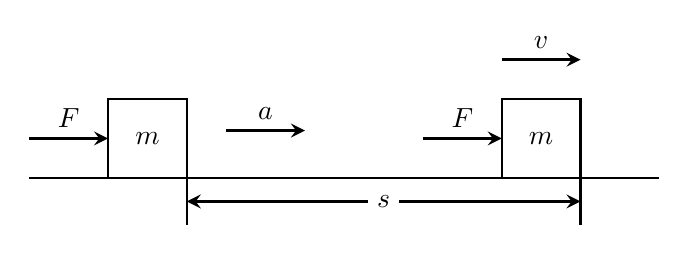
\begin{tikzpicture}[>=stealth, thick]
\draw (0,0)--(8,0);
\draw (1,0) rectangle (2,1);  \draw (6,0) rectangle (7,1);
\node at (1.5,.5){$m$}; \node at (6.5,.5){$m$};
\draw[->, very thick](0,.5)--node [above]{$F$}(1,.5);  \draw[->, very thick](5,.5)--node [above]{$F$}(6,.5);
\draw[->, very thick](2.5,.6)--node [above]{$a$}(3.5,.6);
\draw[->, very thick](6,1.5)--node [above]{$v$}(7,1.5);
\draw (2,0)--(2,-.6);
\draw (7,0)--(7,-.6);
\draw[<->, very thick](2,-.3)--node [fill=white]{$s$}(7,-.3);

\end{tikzpicture}
\caption{}
\end{figure}

设一个原来静止的物体,质量为$m$,由于物体是静止的,没有运动,也就是没有动能,或者说动能为零,在恒定的外力$F$作用下,物体发生一段位移$s$,得到速度$v$(图7.6),获得一定的动能.设外力方向与运动方向相同,外力对物体所做的功$W=Fs$.根据牛顿第二定律,$F=ma$;根据运动学公式$v^2=2as$得到$s=v^2/2a$.将$F$和$s$的表达式代入$W=Fs$中得到
\[W=Fs=ma\times \frac{v^2}{2a}=\frac{1}{2}mv^2 \]

我们看到,外力对物体所做的功等于$\dfrac{1}{2}mv^2$这样一个跟
物体的质量和速度都有关的物理量,在物理学里就用$\dfrac{1}{2}mv^2$
这个物理量来表示物体的\textbf{动能},如果用$E_K$表示动能,那么	
\[E_K=\frac{1}{2}mv^2 \]
这就是说,\textit{物体的动能等于它的质量跟它的速度平方的乘积的一半}.

动能和功一样,也是标量.动能的单位跟功的单位相同,
在国际单位制里都是焦耳,这是因为
\[1[{\rm kg}\cdot {\rm m^2}/{\rm s^2}]=1[{\rm kg}\cdot \ms][{\rm m}]=1{\rm N}\cdot {\rm m}=1{\rm J}\]


\subsection*{练习三}
\begin{enumerate}
    \item 1976年3月8日在吉林市降落一场陨石雨,其中最大的一号陨石的质量是1770千克,假设它以45$\ms$的速度撞击地球,计算它触地时的动能.
    \item 我国第一颗人造地球卫星的质量是173千克,速度为7.2${\rm km}/{\rm m}$时,它的动能是多少?
    \item 一个电子以$8.00\times 10^6\ms$的速度运动,质子必须运动得多快,才能使它具有跟电子一样的动能?已知质子的质量是电子的1800倍.
    \item 有甲、乙两个物体,除了下列每一种不同点而外,这两个物体的其他情况都相同.试比较下列每一种情况下它们的动能:
    \begin{enumerate}
        \item 物体甲的速度是物体乙的两倍.
        \item 物体甲向北运动,物体乙向南运动.
        \item 物体甲做直线运动,物体乙做曲线运动.
        \item 物体甲的质量是物体乙的一半.
    \end{enumerate}
\end{enumerate}

\section{动能定理}

现在我们来进一步证明,如果物体原来就是运动的,已经具有一定的动能,受到外力推动而做加速运动,速度变大,动能增加,这时外力对物体做的功将等于物体动能的增加.

设一个质量为$m$的物体,原来的速度是$v_1$,动能是$\dfrac{1}{2}mv^2_1$,在恒定的外力$F$作用下,发生一段位移$s$,速度增加到$v_2$,动能增加到$\dfrac{1}{2}mv^2_2$.设外力方向与运动方向相同,外力$F$对物体所做的功$W=Fs$.根据牛顿第二定律,$F=ma$;根据运动学公式$v^2_2-v^2_1=2as$得到$s=(v^2_2-v^2_1)/2a$,所以
\[Fs=ma\times \frac{v^2_2-v^2_1}{2a}=\frac{1}{2}mv^2_2-\frac{1}{2}mv^2_1 \]
或
\[W=E_{K2}-E_{K1}\]

可见,\textit{外力对物体所做的功的确等于物体动能的增加}.

上面我们设外力方向与运动方向相同,导出了关系式$E=E_{K2}-E_{K1}$.这个结论对外力方向与运动方向相反的情形同样适用.在这种情形下,外力所做的功是负值,而物体的运动速度减小,动能的增加也是负值.我们知道,外力对物体做负功,往往说成物体克服这个力做了功.因此,对这种情形,也可以说物体克服阻力所做的功等于动能的减少.例如在粗糙平面上运动的小车,在滑动摩擦力的作用下速度减小,这时动能的减少就等于它克服摩擦力所的功.	
	
上述结论是假定物体只受一个力而推导出来的;如物体不只受到一个力,而是受到几个力,上述结论仍旧正确.只是外力所做的功是指各个力所做的功的代数和,即外力所做的总功.这样,我们得到结论:\textbf{外力对物体所做的总功等于物体动能的增加}.这个结论叫做\textbf{动能定理}.

动能定理是力学中一条重要规律,经常用来解决有关的力学问题.下面举一个例题来说明.


\begin{example}
    一架喷气式飞机的质量为$5.0\times 10^3$千克,受到的推力为$1.8\times 10^4$牛,受到的阻力是它的重量的0.020倍,起飞速度为60$\ms$,求起飞时滑跑的距离.
\end{example}


\begin{solution}
    飞机在水平方向受到的外力是推力$F$和阻力$f$,在外力作用下飞机在跑道上滑跑一段距离$s$,速度达到起飞速度$v$.飞机原来是静止的,$E_{K1}=0$,而$E_{K2}=\dfrac{1}{2}mv^2$.阻力
    $$f=0.020\times 5.0\times 10^{3}\times 9.8{\rm N}=9.8\times 10^2{\rm N}$$
    根据动能定理得到
	\[Fs-fs=\frac{1}{2}mv^2 \]
    所以
    \[\begin{split}
        s&=\frac{mv^2}{2(F-f)}\\
&=\frac{5.0\times 10^{3}\times 60^2}{2\times (1.8\times 10^{4}-9.8\times 10^2)}{\rm m}\\
&=5.3\times 10^{2}{\rm m}
    \end{split}\]
	\end{solution}

    这个例题也可以应用牛顿第二定律和运动学公式来解,请同学们自己做一下.动能定理的公式是在牛顿运动定律和运动学公式的基础上推导出来的,所以同一个题目用这两种方法来解,求得的结果是相同的.由于动能定理不涉及物体
    运动过程中的加速度和时间,因此应用它来解题往往比较方便.

    从例题可以看出,在利用动能定理来解力学问题的时候,先要分析物体的受力情况,并据此列出各个力所做的功,然后即可利用动能定理来求解.
    
    \subsection*{练习四}
    \begin{enumerate}
        \item 使一个物体的速度从零增加$v$,再从$v$增加到$2v$.哪种情况下做的功要多些?为什么?
        \item 在光滑平面上的物体受到沿着平面的两个力$F_1$和
        $F_2$的作用(图7.7).在下列情况下,从静止开始移动2米时,物体获得的动能各是多大?
        \begin{enumerate}
            \item $F_1=10$牛,$F_2=0$;
            \item $F_1=0$,$F_2=10$牛;
            \item $F1=F2=5$牛.
        \end{enumerate}

\begin{figure}[htp]
\centering
\begin{minipage}[t]{0.48\textwidth}
\centering
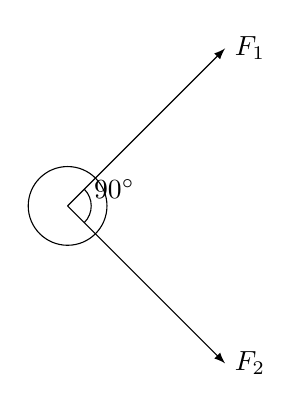
\begin{tikzpicture}[>=latex]
\draw (0,0) circle (.5cm);
\draw[->](0,0)--(2,2)node [right]{$F_1$};
\draw[->](0,0)--(2,-2)node [right]{$F_2$};
\draw (.3,0) arc (0:45:.3)node [right]{$90^\circ$}; 
\draw (.3,0) arc (0:-45:.3); 
\end{tikzpicture}
\caption{}
\end{minipage}
\begin{minipage}[t]{0.48\textwidth}
\centering
\begin{tikzpicture}[>=latex, scale=1.4]
\draw [pattern=north east lines] (-.25,-1.5) rectangle (.25, 1.5);
\draw [|<->|] (-.25, 1.75)--node[above]{$s$} (.25,1.75);
\draw (-1, .1) --(-.6, .1) to [bend left=15] (-.45, 0) to [bend left=15] (-.6,-.1)--(-1,-.1)--(-1,.1); 

\node at (-.7, -.25){$m$};


\draw [dashed] (.5, .1) --(.9, .1) to [bend left=15] (1.05, 0) to [bend left=15] (.9,-.1)--(.5,-.1)--(.5,.1); 

\draw[->] (-1.3, .3)--node[above]{$v_1$}(-.4, .3);
\draw[->] (.4, .3)--node[above]{$v_2$}(1.1, .3);

\draw[->](.2,0)--node[above]{$f$}(-.2,0);

\end{tikzpicture}
\caption{}
\end{minipage}
\end{figure}



    \item 一个30牛的力水平地作用在2.0千克的物体上,使它在无摩擦的水平面上移动了3.0米的距离.然后,这个力变到15牛,又使物体移动了2.0米.物体增加的动能总共是多少?
\item 质量是2.0克的子弹,以300$\ms$的速度水平射入厚度是10毫米的钢板(图7.8),射穿后的速度是100$\ms$.子弹受到的平均阻力是多大?

\item 一架新型喷气式战斗机的质量是$1.50\times 10^4$千克,发动机的推力是$1.11\times 10^5$牛,起飞速度是88.0$\ms$,滑跑距离是671米.计算飞机起飞时受到的平均阻力.
    \end{enumerate}

   \section{重力势能}

   \subsection{重力势能}
   
   动能是和物体运动相联系的,静止的物体没有动能,但不能说它没有能量.除了动能,我们在初中还学过势能.举到高处的重锤具有能量,一旦让它从高处下落,就能够做功,拦河筑坝把水位提高,高处的水下落也能够做功(如水力发电),\textit{物体由于被举高而具有的能叫做重力势能}.举到高处的重锤、储存在高处的水都具有重力势能.

    物体由于被举高才具有重力势能,而物体在举高过程中总是要克服重力做功的.因此,重力势能跟克服重力做功有密切关系.那么,一个质量为$m$的物体,在被举到高度为$h$的
    地方,具有的重力势能是多大呢?

\begin{figure}[htp]
\centering\includegraphics[scale=.45]{fig/7-9.png}
\caption{}
\end{figure}

    我们设想用一个与重力$mg$
    大小相等方向相反的外力$F$把物体举到高处(图7.9).因为物体是在相互平衡的力作用下被举高的,物体的速度没有变化,所以它的动能也没有变化.我们知道,
物体被举高了,它的重力势能要增加,在这个过程中,我们克服重力做了功.克服重力做了多少功,重力势能就增加了多少.把物体举到高度为$h$的地方,克服重力所做的功$W=Fh=mgh$.在物理学里就用$mgh$这个物理量来表示物体的\textbf{重力势能}.如果用$E_P$表示重力势能,那么
\[E_P =mgh\]
这就是说,\textit{物体的重力势能等于它的重量和高度的乘积,惑者说,等于物体的质量、重力加速度、高度三者的乘积}.物体的质量越大,高度越大,它的重力势能就越大.

重力势能也是标量.它的单位也和功的单位相同,在国际单位制中都是焦耳.

\subsection{重力做功与重力势能的变化}

前面讲了,克服重力做了多少功,重力势能就增加多少.例如物体上升,高度增大了,这个过程中克服重力做了功,重力势能就增加了.质量为$m$的物体从高度为$h_1$的地方上升到高度为$h_2$的地方,克服重力做的功是$mg(h_2-h_1)$,重力势能则由$mgh_1$增加到$mgh_2$.反过来,如果重力对物体做了功,重力势能就要减少,例如物体下落,高度减小了,这个过程中重力对物体做了功,重力势能就减少了.质量为$m$的物体从高度为$h_1$的地方降落到高度为$h_2$的地方,重力做的功是$mg(h_1-h_2)$,重力势能则由$mgh_1$减少到$mgh_2$.所以,在物体下落过程中,重力做了多少功,物体的重力势能就减少多少.

\subsection{重力势能的相对性}

我们知道,高度$h$是相对的.我们说某点的高度$h$为若干,这总是相对于一个水平面来说的,这个水平面的高度取作零,例如说珠穆朗玛峰的高度是海拔8848米,这是相对于海平面来说的,海平面的高度取作零.说高山上一座建筑物的高度是5米,那是相对于高山上的一块平地说的.这块平地的高度取作零,测量这座建筑物的高度无需再把海平面的高度取作零.和高度$h$一样,重力势能$mgh$也是相对的.我们说物体具有重力势能$mgh$,这总是相对于某一个水平面来说的,这个水平面的高度取作零,重力势能也是零.这个水平面叫做参考平面,通常选择地面作为参考平面.实际上,选择哪一个水平面作为参考平面,可视研究问题的方便而定.例如研究物体沿斜面的运动,选择通过斜面下端的水平面作为参考平面就比较方便.选择不同的参考平面,物体重力势能的数值是不同的,但这并不影响我们研究问题.我们研究有关重力势能的问题,有确定意义的总是重力势能的差值,而这个差值并不因选择不同的参考平面而有所不同,对选定的参考平面而言,在参考平面上方的物体,高度是正值,重力势能也是正值;在参考平面下方的物体,高度是负值,重力势能也是负值.例如取实验桌的表面作为参考平面(图7.10),在斜面顶端的物体具有正的重力势能$mgh_1$,在地面上的物体具有负的重力旁能$-mgh_2$.说物体具有负的重力势能,只是表示物体在该位置所具有的重力势能比它在参考平面上具有的重力势能要少,这跟用正负温度来表示温度的高低是一样的.关于负的势能我们在今后的学习中将会
碰到.
\begin{figure}[htp]
\centering\includegraphics[scale=.45]{fig/7-10.png}
\caption{正重力势能和负重力势能}
\end{figure}

\section{重力做功的特点和重力势能}
上一节我们讲到了克服重力做了多少功,重力势能就增加了多少;重力对物体做了多少功,重力势能就减少了多少.这个问题还有进一步讨论的必要.为此我们要先研究一下重力做功的特点.

\subsection{重力做功的特点}
\begin{figure}[htp]\centering
\begin{tikzpicture}[>=stealth, thick]
\fill [pattern = north east lines] (-1,-.25) rectangle (6,0);
\draw (-1,0)--(6,0);
\draw (1,4)node[above]{$A$}--(1,1)node[below]{$B$}--(6,1)node[below]{$C$};
\fill (1,4) circle(2pt);\fill (1,1) circle(2pt);\fill (6,1) circle(2pt);
\draw[<->](4,0)--node [fill=white]{$h_2$}(4,1);
\draw[<->](.5,1)--node [fill=white]{$\Delta h$}(.5,4);
\draw[<->](-.5,0)--node [fill=white]{$h_1$}(-.5,4);
\draw (-1,4)--(1,4);
\draw (0,1)--(1,1);
\end{tikzpicture}
\caption{}
\end{figure}

设一个质量是$m$的物体,从原来高度
是$h_1$的$A$点自由下落到高度是$h_2$的$B$点再水平移到$C$点(图7.11),由于物体水平移动中重力并不做功,所以在整个过程中重力对物体所做的功就等于物体由$A$点自由下落到$B$点中重力所做的功:
\[W_G=mg\Delta h=mgh_1-mgh_2\]
如果让这个物体沿着斜面滑下(图7.12),从原来高度是$h_1$的$A$点滑到高度是$h_2$的$C$点,物体沿斜面滑下的距离是$s$,重力所做的功是
\[W_G=mg\sin\theta \cdot s=mg\Delta h=mgh_1-mgh_2\]

\begin{figure}[htp]\centering
\begin{tikzpicture}[>=stealth, thick]
\fill [pattern = north east lines] (-1,-.25) rectangle (6,0);
\draw (-1,0)--(6,0);
\draw (1,4)node[above]{$A$}--(1,1)node[below]{$B$}--(6,1)node[below]{$C$};
\fill (1,4) circle(2pt);\fill (1,1) circle(2pt);\fill (6,1) circle(2pt);
\draw[<->](4,0)--node [fill=white]{$h_2$}(4,1);
\draw[<->](.5,1)--node [fill=white]{$\Delta h$}(.5,4);
\draw[<->](-.5,0)--node [fill=white]{$h_1$}(-.5,4);
\draw (-1,4)--(1,4);
\draw (0,1)--(1,1);
\draw (1,4)--(6,1);
\draw (6-.75,1) arc (180:150:.75)node[left]{$\theta$};

\end{tikzpicture}
\caption{}
\end{figure}



现在我们来看这个物体沿着任一路径$AC$从原来高度是$h_1$的$A$点运动到高度是$h_2$的$B$点,重力所做的功是多少(图7.13).我们把路径$AB$分成许多很短的间隔$AA_1,A_1A_2,A_2A_3,\ldots$,使每个间隔都相当于一个斜面.设每个小斜面的高度是$\Delta h_1,\Delta h_2,\Delta h_3,\ldots$,那么物体通过每个小斜面时重力所做的功是$mg\Delta h_1,mg\Delta h_2,mg\Delta h_3,\ldots$.物体通过路径$AB$时重力所做的功等于重力在每个小斜面上所做的功的代数和,即
\[\begin{split}
W_G&= mg\Delta h_1+mg\Delta h_2+mg\Delta h_3+\cdots\\
&=mg\Delta h\\
&=mgh_1-mgh_2
\end{split} \]

我们看到,\textit{重力对物体所做的功只跟起点$A$和终点$C$的位置有关,而跟物体运动的路径无关.也就是说,只要起点和终点的位置相同,不论物体沿着什么路径运动,重力所做的功都相同}.

这就是重力做功的特点.并不是任何力做功都有这个特点.摩擦力做功就没有这个特点.

\subsection{重力势能的进一步讨论}

\begin{figure}[htp]
    \centering
    \includegraphics[scale=1.2]{fig/7-13.pdf}
    \caption{}
\end{figure}

重力做功的上述特点对于物理学里能够引入重力势能是有决定意义的.原来,如果重力做功没有这个特点,而是与路径有关,那么,我们分别沿着不同的路径把一个物体由地面举到高度为$h$的一点(图7.14),克服重力所做的功将不相同,设沿着路径1把物体举高时克服重力所做的功是$W_1$,沿着路径2把物体举高时克服重力所做的功是$W_2$.这样,位于高度$h$上的物体的重力势能到底等于$W_1$还是等于$W_2$呢?这个重力势能也就没有意义了!可见,正是由于重力做功与路径无关,重力势能的改变才有确定值,在物理学中才可以引入重力势能这个概念.
\begin{figure}[htp]\centering
\begin{tikzpicture}[>=stealth, thick, scale=.8]
\fill [pattern = north east lines] (0,-.25) rectangle (2,0);
\draw (0,0)--(2,0);
\draw [dashed] (1,.25) circle (.25);
\draw [fill=gray!30] (1,5.25) circle (.25);
\draw (1.25,5.25)--(1.75,5.25);
\draw [<->](1.5,5.25)--node [fill=white]{$h$}(1.5,0);

\draw (1,5) [bend right=60] to node [left]{2} (1,.5);
\draw (1,5) [bend right=15] to node [left]{1} (1,.5);

\end{tikzpicture}
\caption{}
\end{figure}

克服摩擦力做的功是与路径有关的.物体沿不同路径从一个位置移到另一位置,克服摩擦力做的功一般是不相等的.
因此,在物理学中就不存在“摩擦势能”这个概念.


\subsection{势能属于系统} 

重力势能的改变是由重力做功来确定的,而重力是地球和物体之间的相互作用力,重力做功涉及的是重力这种相互作用力以及地球和物体的相对位置,所以严格说来,重力势能是地球和物体共有的,而不是物体单独具有的.在物理学中通常把相互作用的物体的全体叫做\textbf{系统},重力势能是属于地球和物体所组成的这个系统的,通常所说的物体具有多少重力势能,只能理解为一种简略的说法.

除了重力势能,还有其他形式的势能,势能是系统由于其中各物体之间存在相互作用而具有的能,而且是由各物体的相对位置决定的.例如分子之间由于存在相互作用而具有由分子间相对位置决定的势能,叫做分子势能.电荷之间由于存在相互作用而具有由电荷间相对位置决定的势能,叫做电
势能.分子势能或电势能分别属于分子或电荷所组成的系统,也不是一个分子或一个电荷单独具有的.

\subsection*{练习五}
下列各题中都以地面作参考平面.
\begin{enumerate}
    \item 体积相同的铝球和铅球,处在同一高度的地方,哪一
    个的重力势能较大?
    \item 质量是2千克的物体位于0.8米高的桌面上,这个物体具有多少重力势能?
    \item 图7.15是几个斜面,它们的高度相同,而倾角不同.
    让质量相同的物体沿斜面从顶端运动到底端,试根据功的公式来计算沿不同斜面重力所做的功,证明这个功跟斜面的倾角无关.
\begin{figure}[htp]
\centering\includegraphics[scale=1.3]{fig/7-15.pdf}
\caption{}
\end{figure}
\item 图7.16表示一个斜抛物体的运动,当物体由抛出位置1运动到最高位置2时,重力所做的功是多少?物体克服重力所做的功是多少?由位置2运动到跟位置1在同一水平面上的位置3时,重力所做的功是多少?由位置1运动到位置3时,重力所做的功是多少?
\end{enumerate}

\begin{figure}[htp]\centering
\begin{tikzpicture}[>=stealth, thick]
\fill [pattern = north east lines] (-1,-.25) rectangle (6,0);
\draw (-1,0)--(6,0);
\draw  (5,0) arc (0:180:2.5);
\draw [fill=gray!30] (0,.25) node {1} circle (.25) ;
\draw [dashed, fill=white] (5,.25) circle (.25) node  {3};
\draw [dashed] (2.5,2.5) circle (.25) node  [above] {2};
\draw [<->] (2.5,2.5)--node [fill=white]{$h$}(2.5,0);
\end{tikzpicture}
\caption{}
\end{figure}


\section{弹性势能}
这一节我们研究物体因发生弹性形变而具有的势能,这种势能叫做\textbf{弹性势能}.物体发生弹性形变的时候,物体的各个部分之间发生弹力的相互作用.正象地球和物体之间由于有重力的相互作用,因而地球和物体组成的系统具有重力势能一样,发生弹性形变的物体的各个部分之间由于有弹力的相互作用,因而由这些部分组成的系统,亦即发生弹性形变的物体本身,就具有弹性势能.

任何发生了弹性形变的物体都具有弹性势能.卷紧了的
发条,拉长或压缩了的弹簧,拉弯了的弓,正在击球的网球拍或羽毛球拍,正在支撑运动员上跳的撑竿等等,都具有弹性势能(图7.17).
\begin{figure}[htp]
\centering\includegraphics[scale=.45]{fig/7-17.png}
\caption{任何发生弹性形变的物体都具有弹性势能}
\end{figure}

弹性势能和弹力做功密切相关,它们的关系类似于重力势能和重力做功的关系,下面以弹簧为例定性地加以说明.

\begin{figure}[htp]\centering
\begin{tikzpicture}[>=latex]
    \tikzstyle{spring1}=[decorate,decoration={aspect=0.5, segment length=3mm, amplitude=3mm,coil}]
    \tikzstyle{spring2}=[decorate,decoration={aspect=0.5, segment length=2mm, amplitude=3mm,coil}]
    \tikzstyle{spring3}=[decorate,decoration={aspect=0.5, segment length=4mm, amplitude=3mm,coil}]
    
    \fill [pattern = north east lines] (-.25,2) rectangle (0,3);
    \fill [pattern = north east lines] (-.25,0) rectangle (0,1);
    \fill [pattern = north east lines] (-.25,-1) rectangle (0,-2);
    
    \draw(0,2)--(0,3);  \draw(0,0)--(0,1);  \draw(0,-1)--(0,-2); 

    \draw [shade] (4, 2.25) rectangle (4.5, 2.75);
    \draw [shade] (3,.25) rectangle  (3.5, .75);
    \draw [shade] (5,-1.75) rectangle  (5.5, -1.25);

    \draw [spring1](0,2.5)--(4,2.5);
    \draw [spring2](0,.5)--(3,.5);
    \draw [spring3](0,-1.5)--(5,-1.5);

 \draw[fill=black] (6.5/2,.5) circle (1.5pt);  \draw [fill=black] (10.5/2,-1.5) circle (1.5pt);
\draw [<->, thick]  (6.5/2+.8,.5)node[right]{$f$}-- (6.5/2-1.1,.5)node[above]{$F$};
\draw [<->, thick]  (10.5/2+1,-1.5)node[right]{$F$}-- (10.5/2-.8,-1.5)node[above]{$f$};
\draw [->] (6.2/2+.3, 1.1)--(6.5/2-.3, 1.1);
\draw [->] (10.5/2-.3, -1.1)--(10.5/2+.3,-1.1);
\end{tikzpicture}
\caption{克服弹力做功,弹簧的弹性势能增加。图中$F$表示外力,$f$表示弹力。上图是没有发生形变的弹簧}
\end{figure}
用外力压缩或伸长弹簧的时候(图7.18),外力要克服弹
力做功,克服弹力做多少功,弹簧的弹性势能就增加多少,把被压缩或伸长的弹簧放开的时候(图7.19),弹力可以推动其他物体做功,弹力做多少功,弹簧的弹性势能就减少多少.
\begin{figure}[htp]\centering
\begin{tikzpicture}[>=latex]
    \tikzstyle{spring1}=[decorate,decoration={aspect=0.5, segment length=3mm, amplitude=3mm,coil}]
    \tikzstyle{spring2}=[decorate,decoration={aspect=0.5, segment length=2mm, amplitude=3mm,coil}]
    \tikzstyle{spring3}=[decorate,decoration={aspect=0.5, segment length=4mm, amplitude=3mm,coil}]
    
    \fill [pattern = north east lines] (-.25,2) rectangle (0,3);
    \fill [pattern = north east lines] (-.25,0) rectangle (0,1);
    \fill [pattern = north east lines] (-.25,-1) rectangle (0,-2);
    
    \draw(0,2)--(0,3);  \draw(0,0)--(0,1);  \draw(0,-1)--(0,-2); 

    \draw [shade] (4, 2.25) rectangle (4.5, 2.75);
    \draw [shade] (3,.25) rectangle  (3.5, .75);
    \draw [shade] (5,-1.75) rectangle  (5.5, -1.25);

    \draw [spring1](0,2.5)--(4,2.5);
    \draw [spring2](0,.5)--(3,.5);
    \draw [spring3](0,-1.5)--(5,-1.5);

 \draw[fill=black] (6.5/2,.5) circle (1.5pt);  \draw [fill=black] (10.5/2,-1.5) circle (1.5pt);
\draw [<-, thick]  (6.5/2+.8,.5)node[right]{$f$}-- (6.5/2,.5);
\draw [->, thick]  (10.5/2,-1.5)-- (10.5/2-.8,-1.5)node[above]{$f'$};
\draw [<-] (6.2/2+.3, 1.1)--(6.5/2-.3, 1.1);
\draw [<-] (10.5/2-.3, -1.1)--(10.5/2+.3,-1.1);
\end{tikzpicture}
\caption{弹力做功,弹簧的弹性势能减少。图中$f$表示弹力。上图是没有发生形变的弹簧}
\end{figure}

弹簧的弹性势能跟弹簧被压缩或拉伸的长度有关系.一
个没有被压缩或拉伸的弹簧,弹性势能为零,弹簧被压缩或拉伸的时候,它被压缩或拉伸得越大,克服弹力所做的功越多,弹簧的弹性势能就越大.另外,弹簧的弹性势能还跟弹簧的倔强系数有关系.不同的弹簧被压缩或拉伸相同的长度,倔强系数越大,克服弹力做的功越多,因而弹簧的弹性势能就越大.

\section{机械能守恒定律}
\subsection{机械能的相互转化}

动能和势能(重力势能和弹性势能)统称为\textbf{机械能}.一种形式的机械能是可以和另一种形式的机械能相互转化的,下面我们看一些例子.

物体自由下落或者沿着光滑斜面滑下的时候,重力对物
体做功,物体的重力势能减少,而物体的速度越来越大,表示物体的动能增加了.这时重力势能转化成动能.

原来具有一定速度的物体,在竖直上升或者沿着光滑斜面上升的时候,物体克服重力做功,速度越来越小,物体的动能减少了,同时物体的高度增加,重力势能增加了.这时动能转化成重力势能.

弹性势能也可以跟动能相互转化.放开一个被压缩的弹簧,它可以把一个跟它接触的小球弹出去.这时弹力做功,弹簧的弹性势能减少,同时小球得到一定的速度,动能增加.放开被拉开的弓把箭射出去,这时弓的弹性势能减少,箭的动能增加.

从这些例子我们看到,机械能的相互转化是通过重力或弹力做功来实现的.重力或弹力做功的过程,也就是机械能从一种形式转化成另一种形式的过程.下面我们进一步来研究
重力或弹力做功的多少跟这种转化的定量关系.
	
\subsection{机械能的守恒} 
\begin{figure}[htp]\centering
\begin{tikzpicture}
[>=stealth, thick]
\fill [pattern = north east lines] (-.5,-.25) rectangle (1.5,0);
\draw (-.5,0)--(1.5,0);
\draw [fill=gray!30] (1,5) node {1} circle (.25) ;
\draw [fill=gray!30] (1,2) node {2} circle (.25) ;
\draw (.75,5)--(.25,5);
\draw (.75,2)--(-.25,2);
\draw [<->] (.5,5)--node[fill=white] {$h_1$} (.5,0);
\draw [<->]  (.15,2)--node[fill=white] {$h_2$} (.15,0);

\draw [->](1,4.75)--node[right] {$v_1$} (1,4.25);
\draw [->](1,1.75)--node[right] {$v_2$} (1,1.25);
\end{tikzpicture}
\caption{}
\end{figure}

我们先用自由落体作例子定量的研究动能和重力势能的转化(图7.20).设有一个质量是$m$的物体,从高度是$h_1$的地方(起点)下落到高度是$h_2$的地方(终点).设
物体在起点的速度为$v_1$,在终点的速度为$v_2$.物体在下落过程中,重力做了功,从动能定理知道,重力所做的功等于物体动能的增加,即
\[W_G=\frac{1}{2}mv_2^2-\frac{1}{2}mv^2_1 \]
另一方面,从重力做功与重力势能的关系知道,重力所做的功等于重力势能的减少,即
\[W_G=mgh_1-mgh_2\]
这样,我们得到
\[\frac{1}{2}mv_2^2-\frac{1}{2}mv^2_1 =mgh_1-mgh_2\]
这就是说,重力做了多少功,就有多少重力势能转化成等量的动能.把上式移项后得到
\[ \frac{1}{2}mv^2_2 +mgh_2=\frac{1}{2}mv^2_1 +mgh_1\]
上式表示,物体在自由下落中,它的重力势能转化成动能,但在任何时刻,动能和重力势能之和亦即它的机械能保持不变.

上述结论不仅对自由落体是正确的,可以证明,在只有重力做功的情形下,它总是正确的.所谓只有重力做功,是指:物体只受重力,不受其他的力,如自由落体和各种抛体运动的情形;或者除重力而外还受其他的力,但其他力并不做功,物体沿光滑斜面运动就属于这种情形.

\textbf{在只有重力做功的情形下,物体的动能和重力势能发生相互转化,但总的机械能保持不变}.这个结论叫做\textbf{机械能守恒定律},它是力学中一条重要规律,又是更普遍的能的转化和
守恒定律的一个特例.

不但动能和重力势能的相互转化中机械能保持不变,在弹性势能和动能的相互转化中,如果只有弹力做功,机械能也是保持不变的.

\subsection*{练习六}
\begin{enumerate}
    \item 在下面列举的各个实例中,除(1)外都不计空气阻力,哪些机械能是守恒的?说明理由.
    \begin{enumerate}[(1)]
        \item 跳伞员带着张开的降落伞在空气中匀速下落.
        \item 抛出的手榴弹或标枪做斜抛运动.
        \item 用细绳拴着一个小球,绳的一端固定,使小球在光滑的水平面上做匀速圆周运动.
        \item 用细绳拴着一个小球,绳的一端固定,使小球在竖直平面上做圆周运动.
        \item 物体沿着光滑的曲面滑下(图7.21甲).
        \item 拉着一个物体沿着光滑的斜面匀速上升(图7.21乙).
        \item 在光滑水平面上运动的小球,碰到弹簧上,把弹簧压缩后又被弹簧弹回来(图7.21丙).
    \end{enumerate}
\begin{figure}[htp]
\centering\includegraphics[scale=.45]{fig/7-21.png}
\caption{}
\end{figure}

    \item  做下面的实验,把物体拴在细线上悬挂起来,做成
    一个单摆(图7.22).把物体从平衡位置$O$拉到$B$,放手后观察物体的来回摆动,把铅笔放在位置1和2,可以看到物体仍然要升到跟$B$同样高的$C_1$和$C_2$.解释这个现象.
\begin{figure}[htp]
\centering
\begin{tikzpicture}[>=latex]
    \fill [pattern = north east lines] (-.5,0) rectangle (.5,0.2);
\draw (-.5,0)--(.5,0);
    \draw (0,0)--(0,-4);
    \draw (0,-.5) arc (-90:-45:.5)node[below]{$\theta$};
    \draw [dashed] (0,0)--(-45:4)--(-135:4)--(0,0);
    \draw[dashed] (0,-4) arc (-90:-45:4);
    \draw[dashed] (0,-4) arc (-90:-135:4);

    \draw[dashed] (0,-1) --(-2.2,-4/1.414);
\draw[dashed] (0,-2) --(-1.5,-4/1.414);
\draw[dashed] (-2.2,-4/1.414) to [bend right=25] (0,-4);
\draw[dashed] (-1.6,-4/1.414) to [bend right=30] (0,-4);

\draw[fill=black] (0,-1) circle (1.5pt)node[right]{1};
\draw[fill=black] (0,-2) circle (1.5pt)node[right]{2};

\draw [fill=white] (-45:4) circle (3pt)node[below]{$B$};
\draw [fill=white] (-135:4) circle (3pt)node[above]{$C$};
\draw [fill=white] (0,-4) circle (3pt)node[below]{$O$};
\draw [fill=white] (-2.2,-4/1.414) circle (3pt)node[above]{$C_1$};
\draw [fill=white] (-1.6,-4/1.414) circle (3pt)node[above]{$C_2$};

\draw [|<->|](.18,.18) to node [fill=white]{$\ell$} (2*1.414+.18, -2*1.414+.18) ;

\end{tikzpicture}
\caption{}
\end{figure}
\end{enumerate}

\section{机械能守恒定律的应用}

机械能守恒定律广泛用来解决各种力学问题,下面通过例题来说明它的应用.


\begin{example}
    竖直上抛的物体,初速度是$v_0$,求物体上升的最大高度.不计空气阻力.
\end{example}


\begin{solution}
    这个问题我们在第二章已经研究过:现在用机械能守恒
定律来处理.竖直上抛的物体只受重力的作用,因而机械能守恒.

物体抛出时,动能是$\dfrac{1}{2}mv^2_0$ ,重力势能为零,机械能$E_1=\dfrac{1}{2}mv^2_0$.物体达到最大高度$H$时,动能为零,重力势能是$mgH$,机械能$E_2=mgH$.因为$E1=E2$,所以
\[\begin{split}
    mgH&=\dfrac{1}{2}mv^2_0\\
    H&=\frac{v^2_0}{2g}
\end{split}\]
\end{solution}

我们看到,用机械能守恒定律求得的答案跟我们在第二章用运动学的方法求得的结果完全相同.

用机械能守恒定律不但能处理直线运动问题,而且能处理曲线运动问题.直接应用牛顿第二定律和运动学的知识来处理力学问题特别是曲线运动,固然可以确定运动物体在任一时刻的位置和速度,从而获得关于这个力学问题的全面知
识,但往往需要用高等数学来计算,有的计算还相当复杂,用机械能守恒定律来处理,却可以相当简便.


\begin{example}
    一个摆长是$\ell$的单摆,最大偏角是$\theta$,求单摆在最低位置的速度(图7.22).
\end{example}


\begin{solution}
    这个问题直接用牛顿第二定律和运动学的知识来处理,就需要用高等数学,现在用机械能守恒定律来处理.

摆链受到两个力:重力和悬线的拉力,悬线的拉力始终垂直于摆锤的运动方向,不做功,所以单摆的机械能守恒.

选择摆锤在最低点时所在的水平面作参考平面,摆锤在最高点时,动能为零,重力势能是$mg(\ell-\ell\cos\theta)$,机械能$E_1=mg(l-\ell\cos\theta)$. 摆锤在最低点时,动能是$\dfrac{1}{2}mv^2$,重力势能
为零,机械能$E_2=\dfrac{1}{2}mv^2$.因为$E_1=E_2$,所以
\[\begin{split}
    \dfrac{1}{2}mv^2&=mg(\ell-\ell\cos\theta)\\
    v&=\sqrt{2g\ell(1-\cos\theta)}
\end{split}\]
\end{solution}

我们看到,由于机械能守恒定律只涉及开始状态和终了状态的机械能,不涉及中间运动过程的细节,因此用它来处理问题相当简便.

当然,有的问题只用机械能守恒定律还不能完全解决.例如要想求单摆在最低位置时悬线的拉力$F$,就还需要应用圆周运动的知识,应用机械能守恒定律求出速度$v$之后,我们不难求出悬线的拉力:
\[F=mg+\frac{mv^2}{\ell}=mg-2mg (1-\cos\theta)\]

解决力学问题,先从能量的观点入手分析,往往带来方便,应用机械能守恒定律来解决力学问题,也要先分析物体的受力情况.在动能和重力势能的相互转化中,如果只有重力做功,其他力不做功,就可以应用机械能守恒定律.

守恒定律不仅给处理问题带来方便,而且有更深刻的意义.物理世界是千变万化的,但是人们发现有些物理量在一定条件下是守恒的,可以用这些“守恒量”来表示物理世界变化的规律,这就是守恒定律.机械能守恒定律就是其中一个,正因为自然界存在着“守恒量”,而且某些守恒定律的适用范围很广泛,所以在物理学中寻求“守恒量”已经成为物理研究工作的一个重要方面,下一章我们将学习另一个守恒定律——动量守恒定律.

\subsection*{练习七}
\begin{enumerate}
    \item 滑雪运动员从25米高的山坡上滑下,如果阻力忽略不计,他滑到坡底时的速度是多大?
    \item 物体从高的光滑斜面的顶端滑下,证明物体到达斜面末端时的速度 $v=\sqrt{2gH}$.
    \item 蒸汽打桩机的重锤的质量是250千克,把它提升到离地面25米高处,然后让它自由落下.计算:
    \begin{enumerate}
        \item 重锤在最高点的动能、重力势能和机械能.
        \item 重锤下落10米时的重力势能、动能和速度.
        \item 重锤落到地面时的重力势能、动能和速度.
    \end{enumerate}
\item 要使一球着地后回跳的高度超过原高10米,必须以多大速度将它下抛?不计球击地时的能量损失.
\item 一个物体从距地面40米的高处自由落下,经过几秒后,该物体的动能和重力势能相等?$g=10\msq$.
\end{enumerate}

\section{功和能}
前面我们研究了机械能的守恒,但是我们经常可以看到机械能并不守恒的事例.仔细考察这类事例可以发现,如果除了重力还有其他力对物体做功,物体的动能和重力势能之和,即物体的机械能,就发生变化.

火车在水平的轨道上开出,重力势能没有变化,动能越来越大,机械能在不断增加.火车机械能的增加是因为牵引力对它做了功,牵引力做多少功,火车的机械能就增加多少.

起重机加速提升重物,重物的动能和重力势能都越来越大,机械能在不断增加.重物机械能的增加是因为钢索的拉力对它做了功,拉力做多少功,重物的机械能就增加多少.

跳伞员在张开降落伞后匀速下降,动能没有变化,重力势
能越来越小,他的机械能在不断减少.跳伞员机械能的减少是因为他克服空气阻力做了功.克服空气阻力做了多少功,机械能就减少多少.

子弹射入墙壁,最后停在墙里,子弹的机械能减少.子弹机械能的减少是因为它克服摩擦力做了功.克服摩擦力做了多少功,机械能就减少多少.

总之,\textit{物体的机械能发生变化,都是因为其他力对物体做了功;其他力做多少功,机械能就增加多少,克服其他力做多少功,机械能就减少多少}.

增加了的机械能并不是凭空产生的.飞机、火车、汽车开动的时候,发动机的牵引力做功,它们的机械能增加了,同时也消耗了燃料中储存的化学能.牵引力做功的过程,就是化学能转化成机械能的过程,牵引力做多少功,就有多少化学能转化成机械能.

减少的机械能也不能无影无踪地消失.子弹射入墙壁的时候,克服摩擦力做功,它的机械能减少,同时产生了热能,使子弹和墙壁的温度升高.克服摩擦力做功的过程,就是机械能转化成热能的过程.克服摩擦力做多少功,就有多少机械能转化成热能.

能量既不能凭空产生,也不能无影无踪地消失,不同形式的能在相互转化中保持守恒.做功的过程就是能从一种形式转化成另一种形式的过程.在机械能不守恒的运动中,做了多少功,就有多少机械能和其他形式的能发生转化.\textit{功是能的转化的量度}.

\section*{复习题}
\begin{enumerate}
    \item 做功的两个不可缺少的因素是什么?计算功的公式是什么?
    \item 什么叫功率?写出计算功率的公式.
    \item 什么叫动能?定义动能的公式是什么?
    \item 动能定理的内容是什么?写出它的公式.
    \item 什么叫重力势能?定义重力势能的公式是什么?
    \item 重力做功有什么特点?这个特点在引入重力势能上有什么意义?
    \item 什么叫弹性势能?什么叫机械能?
    \item 机械能守恒定律的内容是什么?在什么条件下机械能守恒?
    \item 从能量的观点来分析和处理力学问题有什么好处?谈谈你自己的体会.
    \item 这一章的内容较多,你能不能抓住一个基本思路把这一章的知识联系起来?如果你还做不到这一点,建议你认真地再读一读第三节能量和第十一节功和能这两节的课文.
\end{enumerate}

\section*{习题}
\begin{enumerate}
    \item 一个原来静止的物体,在力$F$的作用下,沿着力的方向移动一段距离$s$,得到速度$v$.如果移动的距离不变,力$F$增大到$n$倍,得到的速度也增大到$n$倍.这话对吗?速度应该增大到多少倍?
    \item 在水平面上有两个质量不同而具有相同动能的物
体,它们所受的阻力相等.这两个物体停止前经过的距离是否相同?停下来所用的时间是否相同?
\item 质量是$m$千克的物体自由落下,在第1秒内和第2秒内物体重力势能的减少各是多少?
\item 从地面竖直上抛一个物体,质量是0.2千克,经过8秒落回原地.物体抛出时的动能是多少?从被抛出到最高点,物体克服重力所做的功是多少?物体上升到最高点时的重力势能是多少?不计空气阻力.
\item 一个人站在10米高的楼上沿斜上方抛出一个小球,初速度的大小是10$\ms$,抛出角是30$^\circ$.小球落地时速度是多大?如果初速度的大小不变,沿斜下方抛出小球,抛射角是45$^\circ$,小球落地时速度是多大?用其他某个角度抛出,结果又怎
样?不计空气阻力.
\item 利用机械能守恒定律,你能算出平抛和斜抛物体通过任意位置时速度的大小吗?怎样计算?
\item 质量是0.25千克的球以2.0$\ms$的速度向右运动,然后沿着图7.23所示的光滑的凹面滚动,这个小球在凹面的右侧能滚上多高?如果在$P$点把球从静止放开,它能滚上多高?
\begin{figure}[htp]\centering
\includegraphics[scale=.45]{fig/7-23.png}
\caption{}
\end{figure}

\item  一颗子弹以700$\ms$的速度打穿第一块木板后,这度减低到500$\ms$.如果让它继续打穿第二块同样的木板,它的速度将变为多大?它能否再打穿第三块同样的木板?
\item  列车经过一段长2.1千米的平直铁路,速度从54$\kmh$增加到72$\kmh$,列车重1400吨,列车受到的阻力
是车重的$k=0.003$倍.求机车的功率.
\item  在一个农村小水电站里,上下游的水位差是3米,每秒钟有0.5${\rm m^3}$的水流过发电机的水轮机,从水轮机流出的水的速度是3$\ms$,上游水的流速忽略不计.设水流能的70\%可以转化成电能,求这个小水电站发出的电功率.
\item  飞机、轮船所受的空气或水的阻力并不是固定的,它跟飞机、轮船的速度有关.当速度很大时,阻力与速度的平方成正比,试证明:这时要把飞机、轮船的最大速度增大到2倍,发动机的额定功率要增大到8倍才行.这就是在增大飞机、轮船等交通工具的速度方面,每取得一个新的成就都很不容易的原因.
\item 一辆汽车沿着平直的道路行驶,遇有紧急情况而刹车,刹车后轮子只滑动不滚动,从刹车开始到汽车停下来,汽车前进12米.已知轮胎与路面之间的滑动摩擦系数$\mu=0.7$.求刹车前汽车的行驶速度,不计空气阻力.
\item 一辆5吨的载重汽车开上一个坡路,坡路长$s=100$米,坡顶和坡底的高度差$h=10$米,汽车上坡前的速度是10$\ms$,上到坡顶时减为5.0$\ms$.汽车受到的摩擦阻力是车重的$k=0.05$倍.求汽车的牵引力.取$g=10\msq$.
 
讨论:在这个题目里,汽车的牵引力做多少功?汽车增加
的机械能是多少?其中动能和重力势能各是多少?克服摩擦而转化成的热能是多少?
\item 一个滑雪的人从高度为$h$的斜坡上由静止开始滑下,然后在水平面滑行一段距离停下来(图7.24).已知斜面的倾角为$\theta$,滑雪板和雪之间的滑动摩擦系数为$\mu$,求滑雪人在水平面上滑行的距离$s_1$.你能不能求出滑雪人通过的水
平距离$s$?其他条件不变,只改变斜坡的倾角$\theta$,水平距离$s$是否改变?为什么?
\begin{figure}[htp]\centering
    \begin{tikzpicture}[>=stealth]
\fill [pattern = north east lines, rotate=-30] (0,-.25) rectangle (4,0);
\draw [rotate=-30](0,0)--(4,0);
\fill [pattern = north east lines] (3.45,-2) rectangle (5.5,-2-.25);
\draw (3.45,-2)--(5.5,-2);

\draw[|<->|] (3.45,-2.5)--node[fill=white]{$s_1$}(5.5,-2.5);
\draw[|<->|] (0,-2.75)--node[fill=white]{$s$}(5.5,-2.75);
\draw[|<->|] (0,0)--node[fill=white]{$h$}(0,-2);
\draw[dashed] (-0.5,-2)--(3.45,-2);
\draw[dashed] (0,-2)--(0,-2.75);
\draw[dashed] (5.5,-2.75)--(5.5,-2.25);
\draw  (3.45-1,-2+.55) node[below] {$\theta$}  arc (145:180:1);
    \end{tikzpicture}
    \caption{}
\end{figure}

\item 要使小球滑到光滑的离心轨道顶端时不落下来(图7.25),至少应使它在斜轨上多高处由静止开始下滑?


\begin{figure}[htp]\centering
    \begin{tikzpicture}[>=stealth, scale=1.2]
\draw (-1,0)--(6,0);
\fill [pattern = north east lines] (-1,-.25) rectangle (6,0);

\draw (0,1) circle(1);
\draw (.275,0)--(5,3);
\draw [|<->|](5,0)--node [fill=white]{$h$}(5,3)node[above]{$m$};
\draw [fill=gray](4.6,3) circle (.2);
\draw [dotted](0,2-.2) circle (.2);

\draw[->](0,1)--node [fill=white]{$R$}+(30:1);
\draw [->](0,2-.2)--(.5,2-.2)node[below]{$v$};
\fill (0,1) circle(1pt);
\fill (0,2-.2) circle(1pt);
    \end{tikzpicture}
    \caption{}
\end{figure}

\end{enumerate}


	
	
	
	
	
	
	
	
	
	
	
	
	
	
	
	 %机械能
	%\chapter{动量}\label{chapter-momentum}


\section{冲量和动量}
一辆汽车,受到不同的牵引力时,从开动到获得一定的速
度,需要的时间不同.牵引力大,需要的时间短,牵引力小,需要的时间长.

现在我们来定量地研究一下这类问题.一个质量为$m$的物体,原来静止,在力$F$的作用下,经过时间$t$,将获得多大的速度?这个问题利用牛顿运动定律很容易解决.物体在力$F$
的作用下得到加速度$a=F/m$,经过时间$t$后,在$t$秒末的速度
$v=at=Ft/m$.由此得到
\[Ft=mv\]

可见,要使原来静止的某物体获得某一速度,可以有不同的方法,既可以用较大的力作用较短的时间,也可以用较小的力作用较长的时间;只要力和力的作用时间的乘积$Ft$相同,这个物体总得到相同的速度.这就是说,对一定质量的物体,力所产生的改变物体速度的效果,是由$Ft$这个物理量决定的,在物理学中,力和力的作用时间的乘积$Ft$叫做力的\textbf{冲量}.

冲量是个矢量,它的方向由力的方向决定.如果在作用时
间内力的方向不变,冲量的方向就是力的方向.冲量的单位由力和时间的单位决定,在国际单位制里,冲量的单位是$\UNsA$.

从上式还可以看出,原来静止的不同的物体,在相同冲量的作用下,它们得到的速度不同,质量大的物体得到的速度小,质量小的物体得到的速度大,但是它们的质量和速度的乘积$mv$却是相同的,都等于它们受到的冲量.在物理学中,质量和速度的乘积$mv$叫做\textbf{动量}.

动量常用符号$p$表示.
动量也是矢量,它的方向就是速度的方向.在国际单位制中,动量的单位是$\UkgmsA$.
动量的单位跟冲量的单位实际上是相同的,由于$1 \UN=1 \Ukgmsq$,所以$1\UNs=1 \Ukgms$.

在物理学里,动量是个很重要的量,经常要用到.动量和速度虽然彼此有关,但含义是不同的.速度是运动学上的一个物理量,它描述物体运动的快慢和方向.只有速度的概念,并不能说明使物体得到这个速度或使以这个速度运动的物体停止下来,需要多大的冲量.为了说明这类问题,就要引入动量的概念,动量是动力学上的一个物理量.例如,要使以相同的速度运动的铅球和乒乓球停止下来,铅球需要的冲量大,就是因为铅球的质量大,动量也大的缘故.

动量既然是矢量,它的加法要服从矢量运算规则,即按照平行四边形法则来进行.
如果物体的运动在同一条直线上,即动量矢量在同一条直线上,那么,在选定一个正方向之后,动量矢量的运算就简化成代数运算了.


\begin{example}
    一个质量是0.1千克的钢球以6.0$\Ums$的速度向右运动,碰到一个坚硬的障碍物后弹回,沿同一直线以6.0$\Ums$的速度向左运动.
    碰撞前后钢球的动量有没有变化?变化了多少?
\end{example}


\begin{solution}
    取向右的方向为正方向,钢球碰到障碍物前,它的速度$v=6.0\Ums$,这时钢球的动量
\[p=mv=6.0 \Ukgms\]
碰到障碍物后,钢球的速度$v'=-6.0\Ums$,这时钢球的动量
\[p'=mv'=-6.0\Ukgms\]
可见钢球的动量发生了变化,钢球动量的变化等于变化后的动量减去变化前的动量,所以钢球动量的变化为
\[p'-p=-12\Ukgms \]
\end{solution}

\subsection*{练习一}
\begin{enumerate}
    \item 用4牛的力推动一个物体,力的作用时间是0.5秒,力的冲量是多少?
    \item 使质量为4吨的汽车,从静止达到20$\Ukmh$的速度,需要多大的冲量?
    \item 质量是25千克以0.5$\Ums$的速度步行的小孩和质量是0.02千克以800$\Ums$的速度飞行的子弹,哪个动量大?
    \item 质量为8克的玻璃弹球以3$\Ums$的速度向左运动,碰到一个物体后弹回,以2$\Ums$的速度沿同一直线向右运动.弹球的动量改变了多少?
    \item 以相同的速度分别向竖直和水平方向抛出两个质量相等的物体,抛出时两个物体的动能是否相等?动量是否相等?
\end{enumerate}

\section{动量定理}
现在我们进一步证明,如果物体原来就是运动的,已经具有一定的动量,在合外力的作用下,经过一段时间,速度要发生变化,因而动量也发生变化,这时,物体所受的合外力的冲量等于它的动量的变化.

设一个质量为$m$的物体,原来的速度是$v$,在恒定的外力作用下得到加速度$a=F/m$,经过时间$t$速度变成$v'$,速度的变化就是$v'-v=at$.
由此可得
\[Ft=mat=mv'-mv\]
由于变化前的动量$p=mv$,变化后的动量$p'=mv'$,所以上式可以改写成
\[Ft=p'-p\]
这就是说,\textbf{物体所受合外力的冲量等于它的动量的变化}.这个结论叫做\textbf{动量定理}.

从动量定理可以知道,如果一个物体的动量的变化是一定的,那么,它受力作用的时间越短,这个力就越大,力作用的时间越长,这个力就越小.利用这个道理可以解释为什么茶杯掉在石头上立即摔碎,掉在软的东西上不易摔碎.茶杯碰到物体以前,以一定的速度运动着,动量为$mv$,碰到物体后,停止运动,动量变为0.在这个过程中,茶杯动量的变化是$-mv$,这个值等于茶杯受到的作用力的冲量.掉在石头上,
茶杯从运动到停止经历的时间短,受到的石头的作用力大,因此碎掉.掉在软的东西上,茶杯从运动到停止经历的时间长,
受到的作用力小,因此不易破碎.搬运玻璃等易碎物品时,在木箱里放些纸屑、刨花等物,可以减少搬运中的损坏,也是这个道理.

动量定理不但适用于恒定的外力,而且适用于随时间而变化的变力.在后一种情况下,动量定理中的力$F$应理解为变力在作用时间内的平均值.


\begin{example}
    用5.0千克的铁锤把道钉打进铁路的枕木里去,打击时铁锤的速度是5.0$\Ums$.如果打击的作用时间是0.01秒,求打击时的平均作用力.不计铁锤的重量.
\end{example}

\begin{figure}[htbp]
    \centering
    \includegraphics{fig/A/8-1.pdf}
    \caption{}\label{fig_A_8-1}
\end{figure}

\begin{solution}
    打击时,铁锤和道钉受到的力如图~\ref{fig_A_8-1} 所示.不计铁锤的重量,只考虑铁锤受到的道钉的作用力$N$.铁锤在这个力的作用下,在$t=0.01$秒内,速度由$v=-5.0\Ums$,变为$v'=0$,这里取竖直向上的方向为正方向.
    应用动量定理就可以求出平均作用力:
\[\begin{split}
    N&=\frac{p'-p}{t}=\frac{mv'-mv}{t}\\
    &=\frac{0-5.0\times (-5.0)}{0.01}\UN\\
    &=2.5\times 10^3 \UN
\end{split}\]
道钉所受的打击力$F$,与铁锤所受的力大小相等,方向相反,也是$2.5\times 10^3$牛.
\end{solution}

讨论:上述计算中没有考虑铁锤的重量,如果把铁锤的
重量也考虑在内,那么,这时道钉所受的打击力是上面算出的打击力加上铁锤的重量.而铁锤的重量
\[G=5.0\times 9.8 \UN=49 \UN \]
与上面算出的打击力$2.5\times 10^3$牛相比,铁锤的重量约为后者的2\%,可见在计算打击过程中的平均作用力时,不考虑铁锤的重量是可以的.

\subsection*{练习二}
\begin{enumerate}
    \item 10千克的物体以10$\Ums$的速度作直线运动,在受到一个恒力作用4.0秒钟后,速度变为反向2.0$\Ums$.求:
     \begin{enumerate}
        \item 物体在受力前和受力后的动量;
        \item 物体受到的冲量;
        \item 力的大小和方向.
    \end{enumerate}
    \item 列车的质量是$2.5\times 10^6$千克,受到的牵引力是$4.0\times 
    10^5$牛,它的速度由10$\Ums$增加到24$\Ums$需要用多少时间?
    \item 一个质量是65千克的人从墙上跳下,以7$\Ums$的速度着地,与地面接触后0.01秒停了下来,地面对他的作用力是多大?如果他着地时弯曲双腿,用了1秒钟才停下来,地面对他的作用力又是多大?
    \item 跳远时,为什么跳在砂坑里比跳在混凝土路面上安全?钉钉子时,为什么要用铁锤而不用橡皮锤?
    \item 质量为4千克的铅球和质量为0.1千克的皮球以相同的速度运动着,要使它们在相同的时间内停下来,作用在铅球上的力和作用在皮球上的力哪个大?为什么?
\end{enumerate}

\section{相互作用的物体的动量变化}\label{sec-A-08-change-in-momentum-of-interacting-objects}
我们经常可以看到,物体在相互作用的时候,它们的动量
会发生变化.例如,在滑冰场上原来静止的两个人,无论谁推谁一下,两人就会向相反的方向运动起来(图~\ref{fig_A_8-2}),他们的动量都发生了变化.又例如,在射击的时候,子弹向前飞出,同时枪身后退,子弹和枪身的动量也都发生了变化.
\begin{figure}[htbp]
    \centering
    \includegraphics{fig/A/8-2.pdf}
    \caption{}\label{fig_A_8-2}
\end{figure}

\begin{figure}[htbp]
    \centering
    \begin{minipage}[t]{0.24\linewidth}
        \centering
        \includegraphics[width=3.3cm]{fig/A/8-3.png}
        \caption{}\label{fig_A_8-3}
    \end{minipage}
    \hfill
    \begin{minipage}[t]{0.24\linewidth}
        \centering
        \includegraphics[width=3.3cm]{fig/A/8-4.png}
        %\caption{两个滑块分离后的闪光照片.闪光照相的快慢是每秒10次.图中的刻度尺标出厘米的数值.}\label{fig_A_8-4}
        \caption{}\label{fig_A_8-4}
    \end{minipage}
    \hfill
    \begin{minipage}[t]{0.24\linewidth}
            \centering
        \includegraphics[width=3.3cm]{fig/A/8-5.png}
        \caption{}\label{fig_A_8-5}
    \end{minipage}
    \hfill
    \begin{minipage}[t]{0.24\linewidth}
        \centering
        \includegraphics[width=3.3cm]{fig/A/8-6.png}
        %\caption{两个滑块粘合前后的闪光照片.闪光照相的快慢是每秒7.5次.图中的刻度尺标出厘米的数值.}\label{fig_A_8-6}
        \caption{}\label{fig_A_8-6}
    \end{minipage}
    \caption*{图~\ref{fig_A_8-4}:两个滑块分离后的闪光照片,闪光照相的快慢是每秒10次,图中的刻度尺标出厘米的数值.图~\ref{fig_A_8-6}:两个滑块粘合前后的闪光照片,闪光照相的快慢是每秒7.5次,图中的刻度尺标出厘米的数值.}
\end{figure}


要进一步知道相互作用的物体的动量变化之间的关系,就要做物理实验.

图~\ref{fig_A_8-3} 是放在水平气垫导轨上的两个挨在一起的滑块,在它们之间有一个用线拴住的弹性金属片.
烧断线以后,两个滑块就向相反方向运动.
图~\ref{fig_A_8-4} 是用闪光照相记录下来的滑块在运动中各个时刻的位置.

在这个实验中,右边大滑块的质量是0.30千克,左边小滑块的质量是0.20千克.
从图~\ref{fig_A_8-4} 可以明显看出,两个滑块向相反的方向运动,在每段相等的时间内,小滑块通过的路程
要大些,这说明小滑块的速度比较大.闪光照相的快慢是每秒10次,利用图中的刻度尺你可以量出每1/10秒滑块的位移,从而得出大滑块的速度是0.59$\Ums$,小滑块的速度是0.89$\Ums$.
因此大滑块的动量是0.18$\Ukgms$,小滑块的动量也是0.18$\Ukgms$.
在实验误差范围内,它们的动量大小相等,方向相反.

上述实验研究的是很特殊的情况:相互作用的物体原来是静止的.如果相互作用物体中一个或两个原来在运动,情况又怎样呢?让我们再来做一个实验.

实验装置如图~\ref{fig_A_8-5} 所示,我们在右边大滑块上贴些油泥,推动它一下,使它向原来静止的小滑块运动,它碰上小滑块以后,它们就粘在一起,共同向前继续运动.
图~\ref{fig_A_8-6} 是它们在粘合前后的闪光照相.

大滑块的质量是0.30千克,小滑块的质量是0.20千克.从图~\ref{fig_A_8-6} 可以明显地看出,两个滑块粘合后,虽然还继续向前运动,但速度比原来大滑块的速度小.
闪光照相的快慢这次是每秒7.5次,用前述方法,我们可以知道原来大滑块的速度是0.71$\Ums$,两个滑块粘合后它们的共同速度是0.43$\Ums$.
因此,大滑块失去的向左的动量是0.084$\Ukgms$,小滑块获得的向左的动量是0.086$\Ukgms$.在实验误差范围内,它们的动量变化也是大小相等、方向相反的.

上述实验还是属于比较特殊的情况:物体在碰撞前后都在同一直线上运动,这种碰撞叫做\textbf{正碰}.
当发生斜碰时,也就是碰撞前后物体不在同一直线上运动时,用实验同样可以证明:碰撞物体的动量的变化也是大小相等、方向相反的.这类实验分析起来比较复杂,这里就不讲了.

\section{动量守恒定律}\label{sec-A-08-law-of-conservation-of-momentum}
在上一节分析的几个实验里,相互作用的物体的动量的
变化总是大小相等、方向相反.当然,只根据少量的事例,是不足以总结出普遍规律的.事实上,早在十七世纪,物理学家就已分析了大量的物体的相互作用,逐步建立了动量的概念,并且发现,在任何情况下相互作用的物体的动量的变化总是大小相等、方向相反的.

上述的结论还可以换一个说法.我们把相互作用的物体的动量的矢量和叫做它们的总动量,由于相互作用的物体的动量的变化总是大小相等,方向相反,所以动量的变化为零,因此物体相互作用前的总动量保持不变,这就是动量守恒.

我们还应该把动量守恒的条件仔细讨论一下.
在相互作用的物体构成的系统里,每个物体,既可以受到来自系统内其他物体的力,也可能受到来自系统外其他物体的力,前者叫做\textbf{内力},后者叫做\textbf{外力}.
以图~\ref{fig_A_8-3} 的滑块为例,每个滑块除了受
到相互作用的内力以外,都还受到向下的重力和向上的支持力,重力和支持力作用在同一滑块上,大小相等,方向相反,合力为零.对图~\ref{fig_A_8-5} 中的系统进行同样的分析,也可以看到系统中的物体受到的外力的合力为零.
外力的合力为零或者整个系统根本不受到外力,就是动量守恒的条件.

由此得出结论:\textbf{系统不受外力或所受外力的合力为零,这个系统的动量就保持不变}.这个结论叫做\textbf{动量守恒定律}.

对于在一条直线上运动的两个物体组成的系统,动量守恒定律的一般表达式为
\[m_1v_1+m_2v_2=m_1v'_1+m_2v'_2 \]
式中的$m_1$、$m_2$分别为两个物体的质量,$v_1$和$v_2$分别为它们原来的速度,$v'_1$和$v'_2$分别为它们相互作用后的速度,等号左
边是两物体原来的总动量,右边是它们相互作用后的总动量.

动量守恒定律是自然界最重要的最普遍的规律之一.下面的几点说明可以使同学们对此有比较具体的理解.

(1)在发生相互作用时,不论相互作用的物体是粘合在一起还是分裂成碎块,不论相互作用的物体作用前后的运动
是否在一条直线上,也不论相互作用的物体发生接触与否,动量守恒定律都是适用的.

(2)这个定律并不限于两个物体的相互作用,一个系统里可以包括任何数目的物体,只要整个系统受到的外力的合力为零,系统的动量就守恒.例如,太阳系里太阳和各行星之间,各个行星相互之间,都有万有引力的作用,而太阳系距离
其他天体很远,可以认为不受外力的作用,因此整个太阳系的总动量是守恒的.

(3)从大到星系的宏观系统,直到小到原子、基本粒子的微观系统,无论相互作用的是什么样的力,是万有引力、弹力、摩擦力也好,是电力、磁力也好,甚至是现在对其本性还不很清楚的原子核内的相互作用力也好,动量守恒定律都是适用的,就是说,原来的动量之和总是等于相互作用后的动量之和.

正是因为这样,动量守恒定律成为人们认识自然、改造自然的重要工具.


\begin{example}
    在列车编组站里,一辆$10^5$千克的货车在平直轨道上以2.0$\Ums$的速度运动,碰上一辆不动的$1.5\times 10^5$千克的货车后,它们接合在一起并一同向前运动,求它们共同前进的速度.
\end{example}


\begin{solution}
    这两辆货车组成的系统,受到的外力——重力和轨道的支持力的合力为零,因此它们的动量守恒.在我们的具体情况里,第二辆货车原来不动,$v_2=0$,两车接合后速度相同,$v'_1=v'_2=v$,其中$v$是接合后的共同速度.所以
\[m_1v_1=(m_1+m_2)v \]
解出$v$得
\[v=\frac{m_1}{m_1+m_2}v_1\]
取第一辆货车原来前进的方向作为正方向,代入数值得到
\[\begin{split}
    v&=\frac{10^5}{10^5+1.5\times 10^5}\times 2\Ums\\
    &=0.8\Ums
\end{split}\]
\end{solution}
$v$是正值,表示两辆车接合后以0.8$\Ums$的速度沿第一辆货车原来运动的方向继续向前运动.


\section*{阅读材料:笛卡尔和动量守恒定律}
动量守恒定律,是最早发现的一条守恒定律,它渊源于十六、七世纪西欧的哲学思想.法国哲学家兼数学、物理学家笛卡尔,对这一定律的发现做出了重要贡献.

观察周围运动着的物体,我们看到它们中的大多数终归会停下来.
跳动的皮球,飞行的子弹,走动的时钟,运转的机器,它们都会停止下来.
看来宇宙间运动的总量似乎在减少.整个宇宙是不是也像一架机器那样,总有一天会停下来呢?但是,千百年来对天体运动的观测,并没有发现宇宙运动有减少的迹象,十六、七世纪的许多哲学家都认为,宇宙间运动的总
量是不会减少的,只要我们能够找到一个合适的物理量来量度运动,就会看到运动的总量是守恒的.
那么,这个合适的物理量到底是什么呢?

法国的哲学家笛卡尔曾经提出,质量和速率的乘积是一个合适的物理量.速率是个没有方向的标量.从第\ref{sec-A-08-change-in-momentum-of-interacting-objects}节的第一个实验可以看出笛卡尔定义的物理量在那个实验里是不守
恒的:两个相互作用的物体,最初是静止的,速率都是零,因而这个物理量的总和也等于零;在相互作用后,两个物体都获得了一定的速率,这个物理量的总和不再是零,比相互作用前增大了.

后来,牛顿把笛卡尔的定义略作修改,即不用质量和速率的乘积,而用质量和速度的乘积,这样就得到量度运动的一个合适的物理量,这个量牛顿叫做“运动量”,现在我们叫做动量.笛卡尔由于忽略了动量的矢量性而没有找到量度运动的合适的物理量,但他的工作给后来的人继续探索打下了很好的基础.


\subsection*{练习三}
\begin{enumerate}
    \item 两个原来静止的在水平面上挨在一起的小车,质量分别是0.5千克和0.2千克,在弹力作用下分开.
    较重的小车以0.8$\Ums$的速度向右运动,求较轻的小车的速度.
    \item 在气垫导轨上,一个质量为600克的滑块以15$\Ucms$的速度赶上另一个质量为400克速度为10$\Ucms$的滑块而发生碰撞,碰撞后两个滑块并在一起,求两个滑块碰撞后的速度.
    \item 一个小孩从静止的小船上水平抛出一个球,球的质量是2.0千克,抛出的速度是20$\Ums$.如果小孩和船的总质量为100千克,球抛出时船得到的速度是多大?
    \item 质量为10克速度为300$\Ums$的子弹,打进质量为
    24克静止在光滑水平面上的木块中,并留在木块里.
    子弹进入木块后,木块运动的速度多大?如果子弹把木块打穿,穿过木块后子弹的速度为100$\Ums$,这时木块的速度多大?
    \item 光滑的水平面上停着一辆平车,有两个人在车上相向而行,在什么情况下平车保持静止?在什么情况下平车要运动,运动的方向由什么决定?
\end{enumerate}

\section{动量守恒定律和牛顿运动定律}
我们刚刚学过动量守恒定律,这个定律和以前学过的牛顿运动定律有什么关系呢?原来,只要把牛顿第二定律和第三定律结合起来,就可以推出动量守恒定律.

如果物体1和物体2分别只受到相互作用的力,物体1受物体2的作用力是$F_{12}$,物体2受物体1的作用力是$F_{21}$,除此之外两个物体都不受其他作用.根据牛顿第三定律,$F_{12}=F_{21}$,而且两个物体受到作用的时间$t$是一样的.
设相互作用前后两物体沿同一直线运动,物体1和物体2相互作用前的速度分别为$v_1$和$v_2$,相互作用后的速度分别为$v'_1$和$v'_2$.利用牛顿第二定律可得
\[\begin{split}
    F_{12}&=m_1a_1=m_1\frac{v'_1-v_1}{t}=\frac{p'_1-p_1}{t}\\
F_{21}&=m_2a_2=m_2\frac{v'_2-v_2}{t}=\frac{p'_2-p_2}{t}
\end{split}\]
上面两个式子中的$p'_1-p_1$和$p'_2-p_2$分别表示物体1和物体2在时间$t$内动量的变化.
由于$F_{12}=-F_{21}$,所以
\[p'_2-p_2=- (p'_1-p_1)\]
由此得
\[p_1+p_2=p'_1+p'_2\]

这就是说,两个物体的总动量在相互作用前后保持不变,即系统的总动量是守恒的.

如果系统内相互作用的物体不只是两个,而是三个或者更多,同样也可证明系统的总动量是守恒的.

可见,牛顿运动定律和动量守恒定律是一致的.我们知道,牛顿运动定律只适用于宏观物体的低速运动,我们说牛顿运动定律和动量守恒定律一致,指的是在牛顿运动定律适用范围内二者一致.
随着物理学的发展,人们认识到动量守恒定律具有更大的普遍性,它的有效性已经超出了经典力学的适用范围.第\ref{sec-A-08-law-of-conservation-of-momentum}节末几点说明中的第(3)点讲的就是这个问题.

动量守恒定律和牛顿运动定律虽然是一致的,但是由于动量守恒定律只涉及相互作用前后物体的运动状态,它告诉我们物体在相互作用前后的总动量保持不变,利用这个定律就可以直接求出物体的速度,而不必去过问物体间相互作用过程的细节,比如作用力和加速度的情况、物体速度的变化
过程等,使问题的处理变得简便.这跟前面讲过的,用机械能守恒定律会使问题的处理变得简便,道理是一样的.

\section{弹性碰撞}


让我们来做图~\ref{fig_A_8-7} 所示的实验.
两个质量相同的钢球分别吊在细绳上,静止时挨在一起.
使$A$球偏开一个角度后放开,它回到原来位置时撞上$B$球.可以看到,碰撞后$A$球静止下来,$B$球摆到与$A$球原来高度几乎相等的高度.当$B$球摆回来撞上$A$球后,$B$球又静止下来,$A$球又摆到与原来差不多的高度上.
这个过程还将继续下去,两个球交替摆动.


\begin{figure}[htbp]
	\centering
	\includegraphics{fig/A/8-7.pdf}
	\caption{}\label{fig_A_8-7}
\end{figure}

大家想一想,为什么碰撞后一个球会停下来而把它的动量完全传递给另一个球?
为什么第一球不向后弹回或者两个球都以较小的速度向前运动?
例如,碰撞前$A$球的速度是$v$,碰撞后它以$-0.5v$的速度弹回,$B$球以$1.5v$的速度向前运动,或碰撞后$A$球以$0.2v$的速度、$B$球以$0.8v$的速度都向前运动,这两种情况都不违反动量守恒定律.
在不违反动量守恒定律的许多种可能的情况中,为什么实际发生的只是我们看到的这一种情况呢?

上述的实验和问题是物理学史上一件著名的事情.
1666年,在成立还不久的英国皇家学会的例会上表演了这个实验并引起了很大的兴趣,随后出现了许多对这一现象的不同的甚至是混乱的解释.
到1668年,才有三位学者作出了正确的说明,其中对这一问题作出完整分析的是荷兰物理学家惠更斯.惠更斯认为,在这种碰撞中,除了动量守恒以外,还有另
一物理量守恒,他指出这个物理量就是当时所说的“活力”$mv^2$.后来人们把“活力”改叫动能,并且把它的定义式由$mv^2$改为$\dfrac{1}{2}mv^2$.

同学们在学过本节的例题之后就可以知道,由于在图~\ref{fig_A_8-7} 的实验中动量和动能都守恒,我们看到的现象是唯一可能发生的现象.

那么,是不是在所有的碰撞中除了动量守恒外,动能都守恒呢?你们只要回顾一下图~\ref{fig_A_8-5} 的实验,比较一下两个滑块在碰撞前后的动能之和,就很容易知道,动能是不守恒的.

所以,并非所有的碰撞动能都守恒.有的碰撞动能守恒,
有的碰撞动能不守恒.
正如惠更斯指出的那样,只有在碰撞后物体不发生永久形变、不裂成碎块、不粘在一起、不发热以及不发生其他内部变化的情况下,动能才是守恒的.
我们把这种动量和动能同时守恒的碰撞叫做\textbf{弹性碰撞}.

大多数的碰撞,动能都不守恒,都要有一部分动能转化成其他形式的能,这样的碰撞叫做\textbf{非弹性碰撞}.在非弹性碰撞中,如果物体在相碰后粘合在一起,这时动能的损失最大,这种碰撞叫做\textbf{完全非弹性碰撞}.

钢球、玻璃球、硬木球等坚硬物体之间的碰撞,其实也并
不是完全的弹性碰撞,在碰撞时动能也是有损失的,只是在通常情况下,动能的损失很小,不到百分之三、四,因此我们可以把它们当成弹性碰撞来处理.真正的弹性碰撞,只有在分子、原子以及更小的粒子之间才会遇到.


\begin{example}
    钢球1的质量为$m_1$,钢球2的质量为$m_2$.
    球2原来静止,球1以速度$v_1$向球2运动,求发生弹性正碰后两球的速度$v'_1$和$v'_2$.
\end{example}


\begin{solution}
    根据题意,由两球组成的系统不受外力作用,所以系统的动量守恒.两球发生正碰,碰撞后两球的运动在同一直线上,我们可以用代数式来进行计算,系统动量守恒的表示式是
\begin{equation}\label{eq_A_8-1}
    m_1v_1=m_1v'_1+m_2v'_2
\end{equation}
由于是弹性碰撞,所以动能守恒,即
\begin{equation}\label{eq_A_8-2}
    \frac{1}{2}m_1v_1^2=\frac{1}{2}m_1{v'}_1^2+\frac{1}{2}m_2{v'}_2^2
\end{equation}

从 \eqref{eq_A_8-1} 式可得
\begin{equation}\label{eq_A_8-3}
    m_1(v_1-v'_1)=m_2v'_2
\end{equation}
从 \eqref{eq_A_8-2} 式可得
\begin{equation}\label{eq_A_8-4}
    \frac{1}{2}m_1(v_1-v'_1)(v_1+v'_1)=\frac{1}{2}m_2{v'}_2^2
\end{equation}
把 \eqref{eq_A_8-3} 式代入 \eqref{eq_A_8-4} 式,可得
\begin{equation}\label{eq_A_8-5}
 v_1+v'_1=v'_2   
\end{equation}
利用 \eqref{eq_A_8-3} 和 \eqref{eq_A_8-5} 两式,可以解出
\begin{equation}\label{eq_A_8-6}
\begin{split}
    v'_1&=\frac{m_1-m_2}{m_1+m_2}v_1\\
    v'_2&=\frac{2m_1}{m_1+m_2}v_1\\
\end{split}
\end{equation}
\end{solution}

上面 \eqref{eq_A_8-6} 式就是我们的答案.如果$m_1>m_2$,算出的$v'_1$和$v'_2$都是正值,表示$v'_1$和$v'_2$都与$v_1$方向相同.
如果$m_1<m_2$,算出的$v'_1$为负值,表示$v'_1$和$v_1$方向相反,钢球1在碰撞后将被弹回.

在 \eqref{eq_A_8-6} 式中如果令$m_1=m_2$,可以看到,$v'_1=0$,$v'_2=v_1$.这就是我们在图~\ref{fig_A_8-7} 的实验中看到的现象.

应该注意的是,利用动量守恒和动能守恒,根据碰撞前的速度,我们只能计算出两个物体发生弹性正碰后的速度.如果发生的是斜碰,虽然是弹性碰撞,也不能这样简单地计算出它们碰撞后的速度.这个问题比较复杂,我们就不讨论了.

\subsection*{练习四}
\begin{enumerate}
\item 两个质量都是3千克的球,各以6$\Ums$的速率相向运动,发生正碰后每个球都以原来的速率向相反方向运动.它们的碰撞是弹性碰撞吗?为什么?
\item 一个1.5千克的物体原来静止,另一个0.5千克的以0.2$\Ums$的速度运动的物体与它发生弹性正碰,求碰撞后两个物体的速度.
\item 甲乙两物体在同一直线上同向运动,甲物体在前,乙物体在后.
甲物体质量为2千克,速度是1$\Ums$;乙物体质量为4千克,速度是3$\Ums$.乙物体追上甲物体发生正碰后,两物体仍沿着原来的方向运动,而甲物体的速度变为3$\Ums$,乙物体的速度变为2$\Ums$.
这两个物体的碰撞是弹性碰撞吗?为什么?
\item 在本节课文的 \eqref{eq_A_8-6} 式中,如果$m_2\gg m_1$,就得到$v'_1\approx -v_1,\; v'_2\approx 0$.这组解的物理意义是什么?
\end{enumerate}


\section{反冲运动}
打炮的时候,炮弹从炮筒中飞出,炮身就向后退.这个现象可以用动量守恒定律来说明.
射击前,炮弹静止在炮筒里,它们的总动量为零,炮弹射出后以很大的速度向前运动,炮弹具有了动量,但是根据动量守恒定律,炮弹和炮筒的动量之和还应该等于零,因此炮身得到与炮弹的动量大小相等、方向相反的动量.
只是由于炮身的质量比炮弹的大得多,所以炮身向后运动的速度很小.
炮身的这种后退运动叫做\textbf{反冲运动}.
炮身的反冲运动是不利的,为了使大炮回到原来的位置并重新瞄准,要花不少时间,这就降低了射击速度.现代的大炮都安装了使大炮在发射后自动迅速复位的装置.
此外,人们还发明了无后座力炮,这种炮在发射时火药气从炮身后面的开口喷出,炮身不受火药气的向后的压力,因此发射时不后退.

反冲运动在科学技术中也有许多重要的应用.
喷气式飞
机、火箭就是利用反冲运动来获得巨大速度的.喷气式飞机通过连续不断地向后喷出气体,可以得到超过音速的飞行速度.
\begin{figure}[htbp]
    \centering
    \includegraphics{fig/A/8-8.pdf}
    \caption{}\label{fig_A_8-8}
\end{figure}

我国早在宋代就发明了火箭.
古代火箭的构造跟现在节日里玩的“起花”相似.在竹筒里装入一些火药,把竹筒捆在
箭杆上,火药点燃后,燃烧生成的气体以很大的速度从筒里向后喷出,竹筒带着箭就向前飞去(图~\ref{fig_A_8-8}).这种火箭在古代曾作兵器用过.

现代火箭的原理跟上面的基本相同,只是构造比较复杂.它主要由壳体和燃料两大部分组成,壳体是圆筒形的,前端是封闭的尖顶,后端有尾喷管.燃料燃烧时产生的高温高压气体以很大的速度从尾部向后喷出,火箭就向前飞去(图~\ref{fig_A_8-9}).

理论计算表明,火箭获得的最终速度主要取决于两个条
件,一个是喷气速度,一个是质量比,即火箭开始飞行时的质量与燃料燃尽时的质量之比.
为了提高喷气速度,需要使用高质量的燃料,目前常用的液体燃料是液氢,用液氧做氧化剂.
质量比与火箭的结构和材料有关系,现代技术能达到的质量比不超过10.在现代技术条件下,用一级火箭还不能达到发射人造卫星所需要的速度.要发射人造卫星,现在都用多级火箭.

多级火箭是由单级火箭组成的(图~\ref{fig_A_8-10}).发射时先点燃第一级火箭,它的燃料用完以后空壳就自动脱离,这时第二级火箭开始工作.
第二级火箭在燃料用完以后空壳也自动脱离,以后又是下一级火箭开始工作.多级火箭在工作中及时把对后面航行没有用的空壳抛掉,使火箭的总质量减少,因此能够达到很高的速度,可以用来发射人造卫星、宇宙飞船和洲际导弹.当然,火箭的级数也不是越多越好,因为级数越多,火箭的构造也越复杂,工作的可靠性也越差.目前,多级火箭一般都是三级的.

\begin{figure}[htbp]
    \centering
    \begin{minipage}[t]{0.48\textwidth}
        \centering
        \includegraphics[width=6.5cm]{fig/A/8-9.png}
        \caption{}\label{fig_A_8-9}
    \end{minipage}
    \hfil
    \begin{minipage}[t]{0.48\textwidth}
        \centering
        \includegraphics{fig/A/8-10.pdf}
        \caption{多级火箭}\label{fig_A_8-10}
\end{minipage}
\end{figure}


现代的火箭,工作时推力的大小很不一样.小的如空对
空导弹的火箭,推力只有几万牛,大的如发射人造卫星的火箭和洲际导弹的火箭,推力可达几百万牛以上.

火箭技术与科学技术和国防的现代化都有很大的关系,
是现代的一门重要尖端技术.
我国已经运用自己研制的火箭多次发射过人造卫星和远程导弹.
我们还要进一步提高火箭技术,尽快地赶上和超过国外的先进水平.我们相信,在同学们中,一定会有人在这一重要领域内为祖国作出卓越的贡献!


\section*{复习题}
\begin{enumerate}
    \item 什么是冲量?什么是动量?冲量一定时,作用力的大小与力的作用时间有什么关系?动量一定时,物体的质量与运动速度之间有什么关系?
    \item 什么是动量定理?
    \item 什么是动量守恒定律?
    \item 什么叫弹性碰撞?什么叫非弹性碰撞?什么叫完全非弹性碰撞?哪种碰撞动能的损失最大?
\end{enumerate}


\section*{习题}
\begin{enumerate}
    \item 质量为1千克的手榴弹以60$^\circ$角斜抛出去,抛出的速度为10$\Ums$.
    手榴弹到达最高点时炸成两块,一块的质量是0.6千克,以15$\Ums$的速度沿原方向运动,求另一块的速度大小和方向.
    \item 对于在一直线上运动的两个物体组成的系统,动量守恒定律的一般表达式为:
\[m_1v_1+m_2v_2=m_1v'_1+m_2v'_2 \]
    在不同情况下,这个表达式往往可以简化为不同形式,试写出下列各种情况下得出的简化的表达式:
\begin{enumerate}
    \item 两个物体原来静止,发生相互作用后分开;
    \item 一个物体原来静止,另一个物体跟它碰撞后粘合在一起并共同沿原来的方向运动;
    \item 一个物体原来静止,另一个运动物体与它正碰后,两物体以不同的速度在原来的直线上运动;
    \item 两个相向运动的物体,相碰后都静止下来.
\end{enumerate}
\item 试证明:两个物体碰撞后,它们的速度变化$\Delta v_1=v'_1-v_1$和$\Delta v_2=v'_2-v_2$跟它们的质量成反比,即
\[\frac{\Delta v_1}{\Delta v_2}=-\frac{m_2}{m_1}\]
并利用所得结果来讨论:很轻的物体(如乒兵球)跟一个很重的物体(如课桌)碰撞后,它们的速度变化有什么特征.
\item 质子的质量是$1.67\times 10^{-27}$千克,速度为$1.0\times 10^7\Ums$,与一个静止的氦核碰撞后,质子以$6.0\times 10^6\Ums$的速度反弹回来,氦核以$4.0\times 10^6\Ums$的速度向前运动.
   \begin{enumerate}
       \item 你能否求出氦核的质量?如果能,是多少?
       \item 你能否求出碰撞时的相互作用力?为什么?
   \end{enumerate}
   \item 两个球以相同的速度相向运动,其中一个球的质量是另一个的三倍.
   相碰后重球停止不动,轻球以二倍的速率弹回,试证明它们发生的是弹性碰撞.
   \item 在光滑水平面上一个质量为0.2千克的小球以5$\Ums$的速度向前运动,途中与另一个质量为0.3千克静止的小球发生正碰.假设碰撞后第二个小球的速度为4.2$\Ums$,你算出的第一个小球的速度是多大?想一想,这种情况真的可能发生吗?这道题的毛病出在哪里?
\begin{figure}[htbp]
    \centering
    \includegraphics{fig/A/8-11.pdf}
    \caption{}\label{fig_A_8-11}
\end{figure}
   \item 一个质量$M=0.2$千克的小球放在高度$h=5$米的直杆顶端(图~\ref{fig_A_8-11}).
   一颗质量$m=0.01$千克的子弹以$v_0=500\Ums$的速度沿水平方向击中小球,并穿过球心,小球落地处离杆的距离$s=20$米.求子弹落地处离杆的距离.子弹的动能有多少转化成了热能?
   \item 一个连同装备共有100千克的宇宙航行员,脱离宇宙飞船后,在离飞船45米处与飞船处于相对静止状态.他带着一个装有0.5千克氧气的贮氧筒,贮氧筒有个可以使氧气以50$\Ums$的速度喷出的喷嘴.
   宇航员必须向着与返回飞船相反的方向释放氧气,才能回到飞船上去,同时又必须保留一部分氧气供他在飞回飞船的途中呼吸.飞行员呼吸的耗氧率为$2.5\times 10^{-4} \Ukgs$.如果他在开始返回的瞬间释放0.1千克的氧气,他能安全回到飞船吗?

\begin{solution}
    宇航员向着与返回飞船相反的方向释放出$m=0.1$
千克的氧气后,他将获得向着飞船运动的速度.要知道宇航员能否安全回到飞船,先要求出它返回飞船需要的时间$t$.取飞船为参照物,向着飞船运动的方向为正方向,氧气释放的速度$v=-50\Ums$.设宇航员获得的速度为$V$,宇航员连同装备的总质量为$M$.原来宇航员相对于飞船是静止的,根据动量守恒定律可得:
\[(M-m)V+mv=0\]
考虑到$M\gg m$,得$MV+mv=0$,所以
\[V=-\frac{mv}{M}\]
设宇航员离飞船的距离为$d$,他返回飞船所需的时间
\[t=\frac{d}{V}=-\frac{Md}{mv}=-\frac{100\times 45}{0.1\times (-50)} \Us =900 \Us \]

宇航员呼吸的耗氧率$R=2.5\times 10^{-4}{\rm kg}/{\rm s}$,在返回飞船这段时间$t$内他呼吸需要的氧气
\[m=Rt=2.5\times 10^{-4}\times 900 \Ukg =0.23 \Ukg \]

他释放0.1千克的氧气后,筒内剩余的氧气是
\[ m_{\text{余}}=0.5 \Ukg - 0.1\Ukg  =0.4 \Ukg \]

由于他剩余的氧气多于他返回途中呼吸所需的氧气,因
此他可以安全返回飞船.
\end{solution}

\item 在上题中,如果宇航员想以最短的时间返回飞船,他开始最多能释放出多少氧气?这时他返回飞船所用的时间是多少?
\item 速度为$10^5 \Ucms $的氦核与静止的质子发生正碰,氦核的质量是质子的4倍,碰撞是弹性的,求碰撞后两个粒子的速度.
\item 一个质量是$m_1$,动能是$E_k$的物体与一个质量是$m_2$的不动的物体正碰.
假定发生的是弹性碰撞,在$m_1=0.01m_2$,$m_1=m_2$,$m_1=100m_2$的情况下,$m_1$传递给$m_2$的动能各是多少?

(有兴趣的同学还可以进一步讨论$m_1$传递给$m_2$的动能最大或最小的条件).

\item 在有些原子反应堆里,要让中子与原子核碰撞,以便把中子的速率迅速降低下来.为此,是选用较重的还是较轻的原子核效果较好?为什么?
\end{enumerate}

 %动量
	%\chapter{机械振动和机械波}\label{chapter-mechanical-vibration-and-wave}


前面我们已经学过:在平衡力作用下的匀速运动,在大小和方向都不变的恒力作用下的匀变速运动,在大小不变而方向改变的向心力作用下的匀速圆周运动.现在我们要学习在大小和方向都改变的力作用下的机械振动,以及机械振动的传播形成的机械波.

到电学、光学部分将学习的交流电、电磁振荡、电磁波、光波,跟机械振动、机械波相比,虽然物理本质不同,有许多特征和规律却是相同的.
因此,机械振动和机械波的知识,对于学习电学、光学、电工学和无线电工学等等也很重要.

这一章的内容较多,我们分三部分学习.第一部分是机械振动,第二部分是机械波,第三部分是声学初步知识.


\section{机械振动}
\subsection{机械振动}

\subsubsection{产生振动的条件} 

\textit{物体(或者物体的一部分)在平衡位置附近来回做往复运动,叫做\textbf{机械振动}},常常简称为振动.挂在弹簧下端的重物的上下振动(图~\ref{fig_A_9-1}),单摆的小球的左右摆动,是振动的典型例子.

\begin{figure}[htbp]
	\centering
	\includegraphics{fig/A/9-1.pdf}
	\caption{弹簧下端的重物的上下振动}\label{fig_A_9-1}
\end{figure}


把挂在弹簧下端的重物从平衡位置$O$拉下再放开,它就从最低点$B$向着平衡位置$O$运动并越过$O$运动到最高点$C$,然后再向着平衡位置$O$运动并越过$O$回到最低点$B$.以后重物在平衡位置附近经过多次重复的上下振动,最后停在平衡位置.
把单摆的小球拉开再放手,小球就在平衡位置附近左右振动,经过多次重复,最后停在平衡位置.击一下鼓或敲一下锣,鼓膜或锣面就在平衡位置附近做起伏振动,经过多次重复,最后停在平衡位置.

为什么物体会做这样的运动呢?从地面竖直上抛的物体能返回地面,是因为受到指向地面的力的作用.与此类似,物体所以能在平衡位置附近做往复运动而不远离,并经多次重复以后还停在平衡位置,是因为受到指向平衡位置的力的作用.
使振动物体回到平衡位置的力叫做\textbf{回复力}.

\textit{每当物体离开平衡位置就会受到回复力的作用,这是产
生振动的第一个必要条件}.
应该注意,回复力也是根据力的效果命名的,它可能是弹力,可能是重力,还可能是它们的合力或分力.
后面将讲到回复力的实例.

同一个单摆,在空气里,由于阻力很小,衰减很慢,可以重复摆动许多次才停下.在水里,阻力相当大,衰减很快,摆不了几次就停下.
在很粘的油里,阻力很大,离开平衡位置的摆球虽然还能缓慢地回到平衡位置,但是到达平衡位置时的速度
实际等于零,所以不会产生振动.
可见,\textit{产生振动的第二个必要条件是阻力足够小}.

\subsubsection{表征振动的物理量}

研究匀速和变速直线运动的时候,解决的问题主要是确定物体在任一时刻的位置和速度.研究振动,同样需要确定物体在任一时刻的位置和速度.
这是二者相同的地方.因此,研究振动也需要位移、速度、加速度等物理量.
但是振动有它自己的特点,需要引入新的物理量来表示这种特点.
至于怎样确定振动物体在任一时刻的位置和速度,因为计算比较复杂,本书就不讲了.

振动是一种往复运动,振动物体的位移不像匀速或变速直线运动那样可以继续增大下去,而是有一个最大位移,否则就不成其为振动了.\textit{振动物体离开平衡位置的最大距离叫做\textbf{振幅}}.图~\ref{fig_A_9-1} 中振动的振幅就等于$OB$或$OC$.振幅是表示振动幅度的大小或振动强弱的物理量.




振动的最大特点是重复性,或者说周期性.
所谓周期性,就是振动物体的位移和速度经过一定时间之后又重复地回到原来的数值.例如在图~\ref{fig_A_9-1} 中,振动物体由$B$点经过$O$到达$C$点,再经过$O$回到$B$点,即完成一次全振动,位移和速度就
重复地回到原来的数值.
\textit{完成一次全振动经过的时间叫做\textbf{周期}}.
周期是表示振动快慢的物理量.

振动的快慢也可以用频率来表示.
\textit{在1秒内完成全振动的次数叫做\textbf{频率}}.
频率的单位是\textbf{赫兹},简称赫,国际符号是Hz.
1秒钟振动1次就是1赫.1秒钟振动$n$次就是$n$赫.

如果用$T$(秒)表示周期,用$f$(赫)表示频率,那么
\[f=\frac{1}{T},\qquad T=\frac{1}{f}\]

振幅、周期或频率是表征整个振动的物理量.一个振动,如果知道了它的振幅、周期或频率,我们就从整体上把握了振动的情况.

\subsection*{练习一}
\begin{enumerate}
    \item 设图~\ref{fig_A_9-1} 中振幅是2厘米.
    完成一次全振动,振动物体通过的路程是多少厘米?如果频率是5赫,振动物体每秒通过的路程是多少厘米?
    \item 设图~\ref{fig_A_9-1} 中振幅是2厘米.
    取竖直向上的方向作为正方向,物体运动到点$C$时对平衡位置的位移是多大?运动到点$B$时对平衡位置的位移又是多大?
\end{enumerate}


\subsection{简谐振动}
振动现象是很普遍的,是多种多样的.
我们怎样着手研究它呢?小鸟从树枝上飞开,树枝就振动起来.
这个现象看来比较简单,可是真要研究它,所要考虑的因素却很复杂,不便于我们着手研究.跟研究其他现象一样,研究振动现象也
要从最简单、最基本的振动来着手.前一节我们说过,产生振动的第一个必要条件是要有回复力的作用.回复力的性质是各种各样的,我们希望着手被研究的那种振动,所受的回复力要比较简单.假如回复力是弹簧的弹力,我们希望弹簧的形变在弹性限度之内,因为这时弹力跟形变成正比.产生振动的第二个必要条件是阻力足够小.既然如此,我们着手研究的时候,暂时就不去考虑阻力,而研究一种无阻力的理想化的振动.
这就是这一节要讲的简谐振动.

这里我们再一次遇到所谓理想化的方法.这是研究物理现象经常采用的方法,这样做的好处是使复杂问题变得简单,便于人们就这种简单情况深入探讨,然后再把暂时被抛开的因素和其他因素考虑进去,逐步由简单到复杂.
简谐振动不但是研究复杂振动的基础,它本身也具有实际意义.
许多复杂的振动在振幅小的情况下可以近似地看作是简谐振动.
一切复杂的振动都可以看作是若干振幅、频率不同的简谐振动合成的.

简谐振动的特点是什么呢?下面我们通过一个典型例子来说明,这个典型例子就是弹簧振子.

\subsubsection{弹簧振子} 

照图~\ref{fig_A_9-2} 那样,把连在一起的弹簧和小球穿在水平杆上,弹簧左端固定在支架上,小球可以在杆上滑动.杆非常光滑,小球滑动时的摩擦力可以忽略.弹簧的质量比小球的小得多,也可以忽略.这样就成了一个弹簧振子.
振子静止在$O$点时,它受的重力和杆的支持力互相平衡,弹簧没有形变因而对它没有弹力作用,$O$点就是振子的平衡位置.把它拉离平衡位置再放开,它就沿水平杆左右振动.


\begin{figure}[htbp]
	\centering
	\includegraphics{fig/A/9-2.pdf}
	\caption{弹簧振子的振动}\label{fig_A_9-2}
\end{figure}


在振子振动过程中,重力和杆的支持力总是互相平衡,对振动不起作用,对振动起作用的只是弹簧作用在振子上的弹力.振子运动到$O$点右侧时,弹簧拉长,振子对平衡位置的位移方向向右,弹簧对振子的弹力方向向左.振子运动到$O$点左侧时,弹簧压缩,振子对平衡位置的位移方向向左,弹簧对振子的弹力方向向右.可见在这个弹簧振子上,总是指向平衡位置的回复力是弹簧对振子的弹力.
这个弹力的方向跟振子对平衡位置的位移方向相反.

根据胡克定律,在振幅不大(弹簧不超出弹性限度)的情况下,弹簧振子回复力$F$的大小跟弹簧伸长或缩短的长度$x$成正比,而这个长度就是振子对平衡位置的位移的大小,因此回复力$F$的大小跟这个位移$x$的大小成正比.刚刚讲过,回复力的方向跟这个位移的方向相反.
这样,用下式就可以把回复力的大小和方向都表示出来:
\[F=-kx\]
式中$k$是比例常数,对于弹簧振子来说,就等于弹簧的倔强系数.式中的负号表示回复力的方向跟位移的方向相反.

这种\textit{在跟对平衡位置的位移成正比而方向相反的回复力
作用下的振动,叫做\textbf{简谐振动}}.

用$m$代表振子的质量,用$a$代表振子的加速度,根据牛顿
第二定律$F=ma$ 可以得到
\[a=-\frac{k}{m}x\]

上式表明,在简谐振动中,加速度也跟位移成正比而方向相反.在图~\ref{fig_A_9-2} 里,当振子从$O$向右运动时,加速度的方向向左,并且随着位移增大而增大,即振子做\textit{变减速}运动.
到速度减小到零时,振子运动到右端最大位移处$B$,加速度也增大到最大值.振子从$B$向$O$运动的过程中,加速度的方向仍向左,并且随位移的减小而减小,即振子做初速度为零的\textit{变加速}运动.当振子回到$O$点时,位移减小到零,加速度也减小到零,而速度增大到最大值,方向向左.由于惯性,振子就以这个速度继续向左运动,在越过$O$点以后,加速度的方向向右,
并且随位移的增大而增大,振子做\textit{变减速}运动.
到速度减小到零时,振子运动到左端最大位移处$C$,加速度也增大到最大值.然后振子从$C$向右运动,加速度的方向仍向右,并且随位移的减小而减小,即振子做初速度为零的\textit{变加速}运动.当振子回到$O$点时,位移、加速度都减小到零,而速度增大到最大值,方向向右.此后将重复上述的过程.

值得注意的是,在简谐振动中速度与加速度的变化不一样,加速度最大时速度等于零,加速度等于零时速度最大.

\subsubsection{简谐振动的周期}

简谐振动的周期跟什么有关呢?在回复力的表示式$F=-kx$中,$k$越大,回复力越大,振子产生的加速度越大,振子来回振动得越快,因而周期越短.在图~\ref{fig_A_9-2} 中用不同倔强系数的弹簧做实验,可以看到倔强系数越大,振子的周期越短.
其次,振子的质量$m$越大,产生的加速度越小,振子来回振动得越慢,因而周期越长.在图~\ref{fig_A_9-2} 中用不同质量的振子做实验,可以看到质量越大,振子的周期越长.

计算表明,弹簧振子的周期由下式确定:
\[T=2\pi\sqrt{\frac{m}{k}} \]
可见,\textit{弹簧振子的周期跟质量的平方根成正比,跟弹簧的倔强系数的平方根成反比,而跟振幅无关}.

上式对其他简谐振动也适用,只是对其他简谐振动,$k$的含义不同了.下一节讲到单摆就可以看出这一点.因此上式就是简谐振动的周期公式.

由周期公式知道,对于一个确定的简谐振动系统来说,$m$和$k$都是恒量,所以$T$也是恒量,只由系统本身的特性决定,叫做系统的\textbf{固有周期}.因为$f=1/T$,所以$f$也只由系统本身的特性决定,叫做系统的\textbf{固有频率}.值得注意的是固有周期和固有频率都跟振幅没有关系.
	
\subsection*{练习二}

\begin{enumerate}
    \item 物体在任意回复力作用下振动,一定是做简谐振动吗?为什么?
    \item 用手拍球,使球在硬地上来回跳动,球的运动是简谐
    振动吗?为什么?
\item 分析图~\ref{fig_A_9-2} 中弹簧振子的运动,并填好表~\ref{tab_A_9-1}.
\begin{table}[htbp]
	\centering
	\caption{}\label{tab_A_9-1}
    \begin{tblr}{vlines,hlines,colspec={lcccc}}
        \SetCell{c} 振子的运动  & $C\to O$ & $O\to B$ & $B\to O$ & $O\to C$\\
        {回复力的方向怎样?\\大小如何变化?}&&&&\\
        {运动的性质\\(加速或减速)}&&&&\\
        {加速度的方向怎样?\\大小如何变化?}&&&&\\
        {速度的方向怎样?\\大小如何变化?}&&&&\\
    \end{tblr}
\end{table}
	\item 图~\ref{fig_A_9-2} 所示的弹簧振子的质量是100克,频率为2赫,求弹簧的倔强系数.
    \item 一个如图~\ref{fig_A_9-2} 所示的弹簧振子的质量是200克,弹簧的倔强系数是$16 \UNslashm$,振幅是2厘米.取水平向右的方向作为正方向.当振子运动到右方最大位移时,回复力和加速度的数值各是多大?当振子运动到左方最大位移时,回复力和加速度的数值又各是多大?这个弹簧振子的周期和频率各是多大?
\end{enumerate}


\subsection{单摆}
\subsubsection{单摆的振动特点}

我们已经知道,在一根细线下端拴一
个小球就做成了一个单摆,但是这不是单摆的严格说法.在物理学里,单摆是实际的摆(例如钟摆)的理想化,是指在一根不
能伸长、又没有质量的线的下端系一质点.利用这个理想化的模型,将使定量研究摆的运动大大简化.

当单摆静止不动时,摆线竖直下垂,摆锤$m$(质点)受的重
力$G=mg$跟摆线对它的拉力$T$互相平衡.

使摆锤偏离平衡位置,然后放开,摆锤就在重力$G$和拉力$T$的作用下,沿着以平衡位置$O$为中点的一段圆弧左右振动.我们来分析摆锤运动到任意一点$P$时的受力情况(图~\ref{fig_A_9-3}).这时摆线与竖直方向的夹角是$\alpha$,重力$G$沿摆线方向的分力$F'$跟
拉力$T$的合力,沿着摆线指向圆心(悬挂点),是使摆锤沿圆弧运动的向心力,它只改变摆锤运动的方向,不改变运动的快慢.因此,在研究摆锤沿圆弧运动的位置变化时,不需要考虑向心力,而只考虑重力沿圆弧切线方向的分力$F$,因为正是这个分力$F$是使摆锤振动的回复力.
\begin{figure}[htbp]
    \centering
    \includegraphics{fig/A/9-3.pdf}
    \caption{单摆运动时的受力分析}\label{fig_A_9-3}
\end{figure}
    
重力$G=mg$沿圆弧切线的分力$F=mg\sin\alpha$.当$\alpha$很小时(5$^\circ$以下),圆弧可以近似地看成直线,分力$F$可以近似地看作沿这条直线作用,$OP$ 就是摆锤偏离平衡位置的位移$x$.设摆长是$\ell$,因为$\sin\alpha\approx x/\ell$,所以
\[F=-\frac{mg}{\ell}x\]
式中负号表示力$F$跟位移$x$的方向相反.由于$m$、$g$、$\ell$都有
一定的数值,$mg/\ell$
可以用一个常数$k$来代替,所以上式可以写成
\[F=-kx\]

可见,\textit{在摆角很小的情况下,单摆振动时回复力跟位移成正比而方向相反,是做简谐振动}.

\subsubsection{单摆的周期公式}

将$k=mg/\ell$代入简谐振动的周期公式,
可以得到
\[T=2\pi\sqrt{\frac{\ell}{g}}\]

这就是单摆的周期公式,它表明\textit{在摆角很小的情况下\footnote{根据周期公式算出的$T$值与实际测定值间的误差,随摆角增大而增大,摆角为7$^\circ$时,误差为0.1\%;15$^\circ$时,0.5\%;28$^\circ$时,1\%.单摆最大摆角一般应小于5$^\circ$.},单摆的周期跟摆长的平方根成正比,跟重力加速度的平方根成反比,而跟摆锤的质量、振幅无关}.

在一定的地点,$g$的值一定,一定摆长的单摆就有恒定不变的周期.摆的这个性质被利用在摆钟上计量时间.相反,如果测出摆长$\ell$和周期$T$,也可以利用单摆的周期公式确定$g$的值.由于单摆的摆长$\ell$和周期$T$都容易测量,所以利用单摆可以很方便地测定重力加速度$g$的值,不像利用自由落体运动测$g$那样麻烦.

\subsection*{练习三}
\begin{enumerate}
    \item 假如把单摆和弹簧振子都从地球移到月球上,它们的振动频率是否改变?为什么?
    \item 两个单摆,它们的摆长的比是1:4,求它们的周期的比.两个单摆,它们的频率的比是1:4,求它们的摆长的比.
    \item 测某地的重力加速度时,用了一个摆长为2米的单摆,测得100次全振动所用的时间是4分44秒.
    这个地方的重力加速度多大?
    \item 假如把上题中的单摆拿到月球上去,月球的重力加速度是1.6$\Umsq$,摆的周期将变为多少秒?
\end{enumerate}

\subsection{相和相差}
拿两个摆长相等的单摆来,把它们的摆锤移到平衡位置的一侧,先后放开手让它们振动起来.这两个摆的摆长相等,振动频率是相同的.振幅可以不同.振幅即使相同,也可以看出它们振动的区别来.它们的振动步调不一致,它们不是同时通过平衡位置,也不是同时运动到同一侧的最大位移.这时我们说这两个摆的相是不同的.
相,又叫做相位、位相或周相.

两个频率相同的简谐振动,如果它们的振动步调一致,我们就说它们的相是相同的,简称为\textbf{同相}.在这种情况下,它们总是同时向同一方向运动,同时经过平衡位置,同时运动到同一侧的最大位移.两个摆长相等的单摆,把它们的摆锤移到
平衡位置的同一侧,同时放开手让它们开始振动,它们的振动就是同相的(图~\ref{fig_A_9-4}).
\begin{figure}[htbp]
    \centering
    \includegraphics{fig/A/9-4.pdf}
    \caption{同相的两个简谐振动}\label{fig_A_9-4}
\end{figure}


多数情况下,两个简谐振动的步调并不一致,即它们的相
不同,或者说它们存在着\textbf{相差}.其中有一种特殊情形,即振动步调正好相反,这种情形叫做\textbf{反相}.两个摆长相等的单摆,一个从平衡位置右侧,另一个从平衡位置左侧同时被释放,它们
的振动步调就正好相反(图~\ref{fig_A_9-5}).它们的运动方向总是相反的;一个从右向左经过平衡位置的时候,另一个正好从左向右经过平衡位置;一个到达左侧最大位移的时候,另一个正好到达右侧的最大位移等等.
\begin{figure}[htbp]
    \centering
    \includegraphics{fig/A/9-5.pdf}
    \caption{反相的两个简谐振动}\label{fig_A_9-5}
\end{figure}

相和相差在振动和波的研究中是很重要的,今后的学习
中常常要提到它们.

\subsection{简谐振动的图像}
物体的运动情况可以用公式来表示,也可以用图像来表示.
我们以前学过,匀速直线运动的位移图像是一条通过原点的直线,简谐振动的位移图像是怎样的呢?
\begin{figure}[htbp]
    \centering
    \includegraphics{fig/A/9-6.pdf}
    \caption{摆的振动图像}\label{fig_A_9-6}
\end{figure}

简谐振动的图像可以利用图~\ref{fig_A_9-6} 所示的装置直接从振动物体得到.把漏斗吊在支架上,下方放一块硬纸板,纸板上画一条直线$Ot$.
先使漏斗静止不动,使$O$点恰好在漏斗的正下
方.然后在漏斗里装满细砂,让它摆动,同时沿着跟摆动垂
直的方向匀速拉动硬纸板.因为每一时刻都从漏斗漏出细砂,所以落在硬纸板上的细砂就记录下各个时刻摆的位置.不断漏下的砂组成连续的砂流,在硬纸板上显示出一条曲线,这条曲线就是以横轴$Ot$表示时间、以纵轴表示对平衡位置的位移的振动图像.可以看到,摆的振动图像是正弦或余弦曲线.实际上,所有简谐振动的图像都是正弦或余弦曲线(图~\ref{fig_A_9-7}).
\begin{figure}[htbp]
    \centering
    \includegraphics{fig/A/9-7.pdf}
    \caption{简谐振动的图像}\label{fig_A_9-7}
\end{figure}

振动图像表示出振子对平衡位置的位移怎样随时间面变
化,它可以告诉我们在任一时刻振子对平衡位置的位移.
可见,振动图像直观地表示出了振动的情况.

在振动图像上还可以表示出振幅和周期.
曲线的最大值等于振幅,相邻两个正(或负)的最大值之间的间隔等于周期.

利用振动图像也可以比较振动的相.图~\ref{fig_A_9-8} 是同相的两个简谐振动的图像,从图像容易看出这两个振动的步调是一致的.图~\ref{fig_A_9-9} 是反相的两个简谐振动的图像,从图像容易看出这两个振动的步调恰好相反.

\begin{figure}[htbp]
    \centering
    \includegraphics{fig/A/9-8.pdf}
    \caption{同相的两个简谐振动的图像(图中的箭头表示振子在该时刻的运动方向)}\label{fig_A_9-8}
\end{figure}

\begin{figure}[htbp]
    \centering
    \includegraphics{fig/A/9-9.pdf}
    \caption{反相的两个简谐振动的图像(图中的箭头表示振子在该时刻的运动方向)}\label{fig_A_9-9}
\end{figure}

在许多实际工作中,例如监测地震,振动图像就是直接从振动体记录得来的.
分析研究得到的图像可以了解振动的许多情况.


\subsection*{练习四}


\begin{enumerate}
    \item 图~\ref{fig_A_9-10} 是一个简谐振动的图像.根据图像确定它的振幅和周期.
    \begin{figure}[htbp]
    	\centering
    	\includegraphics{fig/A/9-10.pdf}
    	\caption{}\label{fig_A_9-10}
    \end{figure}
    
    \item 图~\ref{fig_A_9-10} 的振动图像是一条余弦曲线.
    你能不能应用学过的数学知识算出下列时刻振子对平衡位置的位移?
    \begin{enumerate}
        \item $t=0.5$秒;
        \item $t=1.5$秒.
    \end{enumerate}

    提示:想一想在图~\ref{fig_A_9-10} 中,1秒、2秒等时刻相当于余弦函数的多大的角度.

\end{enumerate}

\subsection{简谐振动的能量}

现在从能量的角度来看一看简谐振动.简谐振动不考虑阻力,振动系统的机械能是守恒的.

以单摆为例,当我们把摆锤从平衡位置$O$拉到$B$点时(图~\ref{fig_A_9-3}),摆锤的位置升高,我们克服重力做了功,做功消耗的能转化为摆锤的重力势能,储存在这个振动系统之中.

把拉到$B$点的摆锤放开后,在回复力作用下,摆锤向左做变加速运动,位置降低,速度增大,重力势能转化为动能.当回到平衡位置$O$时,重力势能减少到零(取平衡位置时的重力
势能为零),动能达到最大值,而且这时的动能就等于摆锤在最大位移时的重力势能.

当摆锤越过平衡位置$O$向着$C$点做变减速运动的过程中,位置升高,速度减小,动能转化为重力势能.当摆锤运动到$C$点时,动能减少到零,重力势能达到最大值,而且等于最初储存在系统中的重力势能.

此后,摆锤又向平衡位置运动,重力势能又转化为动能;过了平衡位置继续向$B$点运动,动能又转化为重力势能.
这种转化重复不息,一直进行下去,而摆锤在任何位置(或任何时刻)的机械能即动能和重力势能之和保持不变,都等于最大
位移处的重力势能.我们最初把摆锤拉到$B$点,摆锤在$B$点的位移越大,位置越高,储存在振动系统中的重力势能越大.可见简谐振动的能量跟振幅有关:振幅越大,简谐振动的能量就越大.

在图~\ref{fig_A_9-2} 所示的弹簧振子里也进行着相似的能量转化过程,只不过跟动能相互转化的不是重力势能而是弹性势能.
当我们把弹簧振子从平衡位置拉到$B$点时,克服弹簧的弹力做了功,做功消耗的能转化为弹性势能储存在振动系统之中.把振子放开,在振动过程中弹性势能和动能相互转化,而且重复不息,一直进行下去.
弹簧振子在任何位置(或任何时刻)的机械能即动能和弹性势能之和保持不变,都等于最大位移处的弹性势能.我们知道,弹簧的弹性势能跟弹簧被拉伸或压缩的长度有关系,这个长度越大,弹性势能也越大.可见,振子在$B$点的位移越大,储存的弹性势能就越大.
在弹簧振子中我们同样看到:振幅越大,简谐振动的能量就越大.

简谐振动是一种理想化的振动,一旦供给振动系统一定的能量来使它开始振动,由于机械能守恒,它就要以一定的振幅永不停息地振动下去.可是实际上振动系统不可避免地要受到摩擦和其他阻力,即受到阻尼的作用.
振动系统克服阻尼作用做功,系统的机械能就要损耗.
这样,机械能随着时间逐渐减少,振动的振幅也逐渐减小.待到机械能耗尽之时,振动就停下来了.这种振幅逐渐减小的振动叫做\textbf{阻尼振动}.图~\ref{fig_A_9-11} 是阻尼振动的图像.

\begin{figure}[htbp]
    \centering
    \includegraphics{fig/A/9-11.pdf}
    \caption{阻尼振动的图像}\label{fig_A_9-11}
\end{figure}

振动系统受到的阻尼越大,振幅减小得越快,振动停下来也越快.阻尼过大将不能产生振动.阻尼越小,振幅减小得越慢.在阻尼很小时,在一段不太长的时间内看不出振幅有明显的减小,就可以把振动系统当作简谐振动来处理.前面关于简谐振动的演示就属于这种情形.

\subsection*{练习五}
分析弹簧振子(图~\ref{fig_A_9-2})和单摆(图~\ref{fig_A_9-3})在振动中能量的转化情况,填好表~\ref{tab_A_9-2}.

\begin{table}[htbp]
	\centering
	\caption{}\label{tab_A_9-2}
    \begin{tblr}{hlines,vlines,colspec={cccccc}}
        \SetCell[c=2]{c} 振子的运动  & & $C\to O$ & $O\to B$ & $B\to O$ & $O\to C$\\
        \SetCell[r=3]{m} {能量的变化 \\(增多或减少)} &
动能  &&&&\\
& 势能&&&&\\
&总能&&&&\\
    \end{tblr}
\end{table}

\subsection{受迫振动~~共振}

\subsubsection{受迫振动}

像弹簧振子和单摆那样,在外力使它们偏离平衡位置后,它们就在系统内部的弹力或重力作用下振动起来,而不再需要其他外力推动,这种振动叫做\textbf{自由振动}.由于阻力不可避免,实际的自由振动必然是阻尼振动,最终要停下来.
怎样才能得到持续的周期性振动呢?

得到持续的周期性振动的最简单的方法,是用周期性外力作用于振动物体.
物体在周期性外力作用下的振动叫做\textbf{受迫振动}.
\begin{figure}[htbp]
    \centering
    \includegraphics{fig/A/9-12.pdf}
    \caption{受迫振动}\label{fig_A_9-12}
\end{figure}

受迫振动的频率跟什么有关系呢?我们用图~\ref{fig_A_9-12} 所示的装置来研究这个问题.匀速地转动把手,把手就给弹簧振子以周期性的策动力,使振子做受迫振动.这个策动力的周期跟把手转动的周期是相同的.用不同的转速匀速转动把手,可以看到,振子做受迫振动的周期总等于策动力的周期.所以,\textit{物体做受迫振动的频率等于策动力的频率,而跟物体的固有频率没有关系}.

利用受迫振动来得到持续的周期性振动的例子是非常多
的.例如缝纫机针持续地上下振动,空气压缩机活塞持续地往
复振动,都是周期性策动力作用的结果.

\subsubsection{共振}

难道物体做受迫振动时它的固有频率对振动毫无影响吗?我们用图~\ref{fig_A_9-13} 所示的装置研究这个问题.

在一根张紧的绳上挂几个摆,其中$A$、$B$、$G$的摆长相等.当$A$摆动的时候,$A$的振动通过张紧的绳给其余各摆施加周期性的策动力,其余各摆就做受迫振动.策动力的频率等于$A$摆的频率,决定于它的摆长.其他各摆的固有频率,也都决定于自己的摆长.可以发现,固有频率跟策动力频率相等的$B$、$G$,振幅最大,固有频率跟策动力频率相差最大的$D$、$E$,振幅最小.

\begin{figure}[htbp]
    \centering
    \begin{minipage}[b]{0.45\textwidth}
        \centering
        \includegraphics{fig/A/9-13.pdf}
        \caption{研究摆的共振}\label{fig_A_9-13}
    \end{minipage}
    \hfil
    \begin{minipage}[b]{0.45\textwidth}
        \centering
        \includegraphics{fig/A/9-14.pdf}
        \caption{共振曲线}\label{fig_A_9-14}
    \end{minipage}
\end{figure}


图~\ref{fig_A_9-14} 的曲线表示出了受迫振动的振幅$A$跟策动力频率$f$的关系:策动力的频率$f$等于振动物体的固有频率$f_{\text{固}}$时振幅最大;策动力的频率跟固有频率相差越大,振幅越小.

\textit{当策动力的频率跟物体的固有频率相等的时候,受迫振动的振幅最大,这种现象叫做\textbf{共振}.}

共振,每个推过秋千的人都有这种经验.秋千是个摆,有
它的固有频率.轻推一下使它微微摆动以后,只要按着它的固有频率周期性地施加推力,每当它往回摆时轻轻推它一下,尽管每次的推力都很小,经过一段时间,秋千也会荡得很高,即发生共振.
这种现象是容易理解的.周期性的策动力跟振动“合拍”时,每一次策动力都跟振动物体的速度方向一致,策动力做的功都是正功,都用来增大振动系统的能量,所以振幅越来越大,直到策动力做功供给振动系统的能量等于克服阻力消耗的能量,振幅才不再增大,即达到最大振幅.当策动力不跟振动“合拍”时,策动力做的功有一部分是负功,因而振动系统从策动力得到的能量比“合拍”时少,振幅也就比“合拍”时小.

共振现象有很多应用.在修建桥梁时需要把管柱插入江底作为基础,如果使打桩机打击管柱的频率跟管柱的固有频率一致,管柱就发生共振而激烈振动,使周围的泥砂松动,于是管柱可以比较容易地插下去.

在某些情况下,共振现象可能造成损害.
例如,当军队或火车过桥的时候,整齐的步伐或车轮对铁轨接头处的撞击,都是周期性的策动力,如果它的频率接近于桥梁的固有频率,就可能使桥的振幅大到桥梁断裂的程度.因此,部队过桥要用便步,以便不产生周期性的策动力.火车过桥要慢开,以便策动力的频率远小于桥的固有频率.又如,轮船航行的时候,会受到周期性的波浪的冲击而左右摇摆.如果这个冲击力的频率跟轮船左右摇摆的固有频率相同,就发生共振,激烈的共振甚至可以使轮船倾覆.这时候可以改变轮船的航行方向和航行速率,使波浪冲击的频率远离轮船摇摆的固有频率.

在需要利用共振的时候,应该使策动力的频率接近或等
于振动系统的固有频率.
在需要防止共振危害的时候,要想办法使策动力频率和固有频率不相等,而且相差尽可能多些.

\subsection*{练习六}
\begin{enumerate}
    \item 除了书上讲过的自由振动和受迫振动的例子外,再各举两个实例.
    \item 仿照图~\ref{fig_A_9-13} 所示的研究共振现象的装置,自己利用手边的材料来做实验,观察受迫振动的振幅跟策动力频率之间的关系.
    \item 汽车的车身是装在弹簧上的,如果它的固有周期是1.5秒,汽车在一条起伏不平的路上行驶,路上各凸起处相隔的距离都大约是8米,那么汽车以多大的速度行驶时车身的起伏振动最激烈?
\end{enumerate}


\section{机械波}
设想在池塘中飘浮一支玩具小船,可以在塘边投一块小石子去击中小船,把能量传给它,使它动一动.也可以用另外的方式传递能量,把一块石子投到塘边的水里,激起一圈圈起伏不平的水波向周围传播开去,传到小船,使它动荡起来.在这个简单的现象中,我们接触到了物理学中一个重要的课题,一种新的传递能量的方式——利用波来传递能量.

我们听到声音,是靠声波把能量传递给我们的耳朵.
远处发生地震,激起的地震波把能量传来,造成危害.打开收音机和电视机,我们听到声音,看到图像,是因为它们接收到电磁波传来的能量和信号.太阳供给地球巨大的能量,使人类得以生存,是靠光波传来的.水波、声波、地震波都是由机械振动引起的机械波,传递机械能.电磁波和光波传递电磁能和光能.
现在我们来学习机械波的知识.


\subsection{机械振动在媒质中的传播——机械波}
\subsubsection{机械波} 

水波是在水中传播的,空气中的声波是在空气中传播的,地震波是在地壳中传播的.借以传播波的物质常常叫做媒质.波要靠媒质来传播,这是机械波的特点.


波为什么会在媒质中传播呢?原来媒质的各部分之间存在着相互作用力,如果媒质的某一部分发生了振动,那么,由于它对周围其他部分有力的作用,就带动周围各部分振动起来.同样,周围各部分又带动较远的各部分振动起来.这样,振动在媒质内不会局限在一个地方,而要在媒质内传播出去.\textit{机械振动在媒质中的传播叫做\textbf{机械波}}.在力学里提到波,通常就是指机械波.

现在稍微细致地看一下机械振动在媒质中是怎样传播的.

照图~\ref{fig_A_9-15} 那样,把绳的一端固定,用手拿着另一端上下振动,就会看到凸凹相间的波向绳的一端传去.
设想把绳分成许多小部分,每一小部分看作质点,质点和质点之间有弹力作用(图~\ref{fig_A_9-15b}).
当质点1在外力作用下振动起来以后,就带动质点2振动起来,不过质点2开始振动的时刻比质点1要迟一些,因而它们振动的相不同.这样依次带动下去,后一个质点总比前一个迟一些开始振动.
在这列质点中,正因为相邻质点振动的相不同,从整体上来看才形成凸凹相间的波向前传播.这里我们看到,绳上的质点都在上下振动,并不随波迁移,沿绳传播的只是振动这种运动形式.

\begin{figure}[htbp]
    \centering
    \begin{subfigure}{0.8\linewidth}
    	\centering
    	\includegraphics{fig/A/9-15a.pdf}
    	\caption{}\label{fig_A_9-15a}
    \end{subfigure}
    \\
    \begin{subfigure}{0.8\linewidth}
    	\centering
    	\includegraphics{fig/A/9-15b.pdf}
    	\caption{}\label{fig_A_9-15b}
    \end{subfigure}
    \caption{沿绳传出凸凹相间的波}\label{fig_A_9-15}
\end{figure}

把一根长的螺旋弹簧用细线水平悬挂起来,在它的一端连接一个金属球,球固定在钢片上(图~\ref{fig_A_9-16a}).
当金属球沿着弹簧方向左右振动时,在弹簧上就有疏密相间的波向右传去.
我们也可以把弹簧看作一列由弹力联系着的质点.金属球振动起来以后,依次带动后面的质点,而且后一个质点也是总比前一个迟一些开始振动,使相邻质点振动的相不同.这里质点是左右振动的,因而从整体上看形成疏密相间的波向前传播(图~\ref{fig_A_9-16b}).质点也不随波迁移,传播的也只是运动形式——振动.

\textit{机械波向外传播的只是运动形式——机械振动,媒质本身并不随波迁移.}

随着波的传来,本来静止的质点开始振动起来,表明它获得了能量.
这个能量是从波源通过前面的质点依次传来的.
所以波在传播振动的同时,也将波源的能量传递出去.
持续地供给波源以能量,就能够持续地从波源以波的形式把能量传递出去.
\textit{波是传递能量的一种方式}.

\subsubsection{横波和纵波} 

按照质点振动方向与波的传播方向之间的关系,可以把波分成横波和纵波.

\textit{振动方向与波的传播方向垂直的波叫做\textbf{横波}}.图~\ref{fig_A_9-15} 所示绳子上的波是横波的例子,质点上下振动,波向右传播,这两个方向互相垂直.

\textit{振动方向与波的传播方向在同一直线上的波叫做\textbf{纵波}}.
图~\ref{fig_A_9-16} 所示沿弹簧传播的疏密波是纵波的例子,质点左右振动,波向右传,这两个方向在同一直线上.
\begin{figure}[htbp]
    \centering
    \begin{subfigure}{0.8\linewidth}
    	\centering
    	\includegraphics{fig/A/9-16a.pdf}
    	\caption{}\label{fig_A_9-16a}
    \end{subfigure}
    \\
    \begin{subfigure}{0.8\linewidth}
    	\centering
    	\includegraphics{fig/A/9-16b.pdf}
    	\caption{}\label{fig_A_9-16b}
    \end{subfigure}
    \caption{沿弹簧传出疏密相间的波}\label{fig_A_9-16}
\end{figure}



发生地震时,从震源传出的地震波,既有横波,又有纵波.

\subsubsection{波长、频率和波速之间的关系}

从图~\ref{fig_A_9-15} 可以看出,在振动传播到质点13以后,质点13的振动跟质点1的振动,步调完全一致:质点1从平衡位置向上动时($t=T$的瞬间),质点13从平衡位置向上动;再过四
分之一周期,质点1向上运动到最大位移处,速度减小到零,质点13也向上运动到最大位移处,速度减小到零.
所以这两个质点的振动同相.
同样,质点2和质点14,质点3和质点15的振动也是同相.

\textit{沿着波的传播方向,两个相邻的同相质点间的距离,叫做波长}.波长通常用字母$\lambda$表示.

图~\ref{fig_A_9-15} 中质点1和质点13间的距离,质点2和质点14间的距离,质点3和质点15间的距离等等,都等于波长.

在横波中,两个相邻的凸部——波峰的中央间的距离,或两个相邻的凹部——波谷的中央间的距离,都等于波长.

从图~\ref{fig_A_9-15} 还可以看出,在质点1振动一周期后质点13开始振动,在质点4振动一周期后质点16开始振动.
可见,在一周期的时间内,振动在媒质中传播的距离等于波长.

既然在一个周期$T$的时间内,振动传播的距离等于波长$\lambda$,那么振动传播的速率——波速$v$可以根据下面的式子求出:
\[v=\frac{\lambda}{T}\]
由于振动周期$T$与振动频率$f$互为倒数,即$T=1/f$,$f=1/T$,所以上面的式子可以写成
\[v=\lambda f\]
即\textit{波速等于波长和频率的乘积}.这个关系,虽然我们是从机械波得到的,但是它对于今后将要学习的电磁波、光波也是适用的.

机械波在媒质中传播的速率是由媒质本身的性质决定的,在不同媒质中传播的速率并不相同.

\subsection*{练习七}
\begin{enumerate}
    \item 在某一地区,地震波的纵波和横波在地表附近的传播速率分别是9.1$\Ukms$和3.7$\Ukms$.在一次地震时,这个地区的一个观测站记录的纵波和横波的到达时刻相差5秒.
    那么地震的震源距这个观测站多远?
    \item 一只船停泊在岸边,如果海浪的波峰间的距离是6米,海浪的波速是1.5$\Ums$,求船摆晃的周期是多少?
    \item 甲乙二人分乘两只船在湖中钓鱼.
    两船相距24米.有一列水波在湖面上传播开来,每只船每分钟上下浮动20次.
    当甲船位于波峰时,乙船位于波谷,这时两船之间还有一个波峰.
    水波的波速是多大?
    \item 仔细研究图~\ref{fig_A_9-15},说明:两个相邻的反相质点间的距离等于波长的多少.
\end{enumerate}

\subsubsection{波的图像}

波的运动情况可以用图像直观地表示出来.反之,知道了一列波的图像,也可以对图像进行分析,从而了解这列波的运动情况.

用横坐标表示在波的传播方向上媒质各质点的平衡位置,纵坐标表示某一时刻各质点的位移矢量,连接各位移矢量
末端得到的曲线,叫做\textbf{波的图像},它表示某一时刻媒质各质点离开平衡位置的情况.
\begin{figure}[htbp]
    \centering
    \begin{subfigure}{0.8\linewidth}
        \centering
        \includegraphics{fig/A/9-17a.pdf}
        \caption{}\label{fig_A_9-17a}
    \end{subfigure}
    \\
    \begin{subfigure}{0.8\linewidth}
        \centering
        \includegraphics{fig/A/9-17b.pdf}
        \caption{}\label{fig_A_9-17b}
    \end{subfigure}
    \caption{横波的图像}\label{fig_A_9-17}
\end{figure}


图~\ref{fig_A_9-17a} 表示某一时刻$t$绳上的一列横波,图~\ref{fig_A_9-17b} 是它的图像.可见图像直观地表现了这列横波在时刻$t$的形状——波形,从图像上可以直接看出各质点在时刻$t$的位移.
如果我们还知道这列波的传播方向和波速$v$,那么可以进一步知道任何时刻,例如再经过$\Delta t$时间以后,波的形状和各质点的位移,办法是照图~\ref{fig_A_9-18} 那样,使波形曲线沿着波的传播方向移动$v\Delta t=\Delta x$一段距离.
\begin{figure}[htbp]
	\centering
	\includegraphics{fig/A/9-18.pdf}
	\caption{时刻$t$及时刻$t+\Delta t$的波形曲线}\label{fig_A_9-18}
\end{figure}


在图~\ref{fig_A_9-19} 中,甲图表示一根没有发生形变的弹簧,上面标出一些质点的平衡位置;乙图表示弹簧中出现纵波时,某一时刻各个质点的位移情况;丙图表示的是这列纵波的图像.图
象中,向上的纵坐标表示质点从平衡位置向右的位移,向下的纵坐标表示质点从平衡位置向左的位移,曲线跟横坐标轴的各个交点,依次表示纵波的密部和疏部的中央.


\begin{figure}[htbp]
    \centering
    \begin{subfigure}{0.8\linewidth}
        \centering
        \includegraphics{fig/A/9-19a.pdf}
        \caption{}\label{fig_A_9-19a}
    \end{subfigure}
    \\
    \begin{subfigure}{0.8\linewidth}
        \centering
        \includegraphics{fig/A/9-19b.pdf}
        \caption{}\label{fig_A_9-19b}
    \end{subfigure}
    \\
    \begin{subfigure}{0.8\linewidth}
        \centering
        \includegraphics{fig/A/9-19c.pdf}
        \caption{}\label{fig_A_9-19c}
    \end{subfigure}
    \caption{纵波的图像.
    横坐标表示各质点所在的平衡位置,纵坐标表示各质点的位移.图中的$x_2$是质点$2$向右的位移,$x_5$是质点$5$向左的位移.}\label{fig_A_9-19}
\end{figure}



把图~\ref{fig_A_9-18} 和图~\ref{fig_A_9-19} 所示的波的图像跟图~\ref{fig_A_9-7} 所示的振动图像相比,会看到它们很相似.实际上,由简谐振动在媒质中传播所形成的波——简谐波,在任何时刻的图像都是正弦(或余弦)曲线,媒质的任何质点的振动图像也都是正弦(或余弦)曲线.例如,图~\ref{fig_A_9-20a} 是在一条绳上传播的简谐波在某一时刻的图像,图~\ref{fig_A_9-20b} 是这列波传播过程中绳上某一点的振动图像.
这两条曲线变化规律相同,都按正弦(或余弦)规律变化,但是它们的物理意义不同.\textit{波的图像表示的是某一时刻各个质点的位移,振动图像表示的是某一质点在各个时刻的
位移}.在波的图像中,相邻两个最大值之间的距离等于波长$\lambda$,在振动图像中,相邻两个最大值之间的间隔等于周期$T$.
\begin{figure}[htbp]
    \centering
    \begin{subfigure}{0.8\linewidth}
        \centering
        \includegraphics{fig/A/9-20a.pdf}
        \caption{一列简谐横波在某一时刻的图像}\label{fig_A_9-20a}
    \end{subfigure}
    \\
    \begin{subfigure}{0.8\linewidth}
        \centering
        \includegraphics{fig/A/9-20b.pdf}
        \caption{绳上某点的振动图像}\label{fig_A_9-20b}
    \end{subfigure}
    \caption{}\label{fig_A_9-20}
\end{figure}

可见,对待图像也必须像对待表示物理概念或规律的公式那样,弄清它的物理意义.

\subsection*{练习八}
\begin{enumerate}
    \item 振动图像和波的图像各表示的是什么内容?振动图像中相邻两个最大值之间的间隔等于什么?波的图像中相邻两个最大值之间的间隔等于什么?
    \item 有一列波,它在某一时刻的波形曲线如图~\ref{fig_A_9-18} 中的实线所示.
    这列波经过$T/4$后的波形曲线是什么样?经过$2T/4$,$3T/4$后又是什么样?
    \item 横波的图像直观地表现了横波在某一时刻的波形,纵波的图像却不能直观地表现纵波的情况,但是,我们看到纵波的图像应该很自然地想出纵波的情况,就像我们看到振动图像应该很自然地想出弹簧振子或单摆的振动情况一样.仔细考察图~\ref{fig_A_9-19},回答下面的问题.
    \begin{enumerate}
        \item 在图像的什么地方质点向右的位移最大?
        \item 在图像的什么地方质点向左的位移最大?
        \item 在图像的什么地方质点的位移为零?
        \item 密部中央两侧质点的位移有什么特征?
        \item 疏部中央两侧质点的位移有什么特征?
    \end{enumerate}
\end{enumerate}

\subsection{波的干涉}
\subsubsection{波的叠加} 

前面研究的只限于从一个波源传出的一列波.但是实际情况是,常常有几列不同的波同时在媒质中传播.例如,把两块石子在不同地方投到池塘的水里,就有两列水波在水面上传播.

两列或几列波相遇,会不会像两个或几个球相碰时那样
改变了它们原来的运动状态呢?实验是回答问题的最好办法.
\begin{figure}[htbp]
    \centering
    \begin{subfigure}{0.8\linewidth}
        \centering
        \includegraphics{fig/A/9-21a.pdf}
        \caption{}\label{fig_A_9-21a}
    \end{subfigure}
    \\
    \begin{subfigure}{0.8\linewidth}
        \centering
        \includegraphics{fig/A/9-21b.pdf}
        \caption{}\label{fig_A_9-21b}
    \end{subfigure}
    \\
    \begin{subfigure}{0.8\linewidth}
        \centering
        \includegraphics{fig/A/9-21c.pdf}
        \caption{}\label{fig_A_9-21c}
    \end{subfigure}
    \\
    \begin{subfigure}{0.8\linewidth}
        \centering
        \includegraphics{fig/A/9-21d.pdf}
        \caption{}\label{fig_A_9-21d}
    \end{subfigure}
    \\
    \begin{subfigure}{0.8\linewidth}
        \centering
        \includegraphics{fig/A/9-21e.pdf}
        \caption{}\label{fig_A_9-21e}
    \end{subfigure}
    \caption{在绳子上两个相遇的波互相穿过}\label{fig_A_9-21}
\end{figure}


一个波源在绳的左端发出波1,另一个波源在绳的右端
发出波2,如果两个波源经过1/2周期后停止振动,就会有如图~\ref{fig_A_9-21a} 那样的两个波分别从绳的两端发出并相向传播.
我们发现两个波在彼此相遇并互相穿过后,波的形状和相遇前一样,传播的情形也和相遇前一样(图~\ref{fig_A_9-21e}),也就是它们都
保持自己的状态而不受相遇波的影响.同样,两列水波互相穿过,仍然保持各自的状态继续传播,就像没跟另一列波相遇一样.

\textit{几列波相遇时能够保持各自的状态而不互相干扰,这是波的一个基本性质.}

两列波相遇互相穿过时,在两列波重叠的区域里的媒质质点的位移将怎样呢?根据运动合成的知识知道,每个质点都同时参与这两列波引起的振动,合振动的位移等于两个分振动引起的位移的矢量和.在图~\ref{fig_A_9-21} 里也可以看出两波重
叠的瞬间(图~\ref{fig_A_9-21c}),最大位移等于两波振幅之和.

\textit{两列波重叠区域里任何一点的总位移,都等于两列波分别引起的位移的矢量和.}

\subsubsection{波的干涉} 

一般地说,振动方向以及振幅、频率、相都不相同的几个波源发出的波互相叠加,情形是很复杂的.我们的讨论只限于振动方向相同的两个波源发出的波的叠加.现在我们讨论一种最简单但是最重要的情形,就是这两列波的频率相同、相也相同(或相差恒定)的情形.

把两根细金属丝固定在薄钢片上,让两根金属丝的下端刚刚接触水波演示槽的水面,当薄钢片振动的时候,两根金属丝就周期性地接触水面,成为两个频率和相都相同的波源,从这两个波源分别发出两列波长相同的水波.我们先根据波的叠加分析一下将发生什么现象,然后用实验来检验.
\begin{figure}[htbp]
    \centering
    \includegraphics{fig/A/9-22.pdf}
    \caption{两个相同波源发出的波的叠加示意图}\label{fig_A_9-22}
\end{figure}

既然每一列波的传播都不受另一列波的干扰,我们就可以照图~\ref{fig_A_9-22} 那样,用两组同心圆弧分别表示从波源$S_1$、$S_2$发出的两列波,实线圆弧表示波峰,虚线圆弧表示波谷.某一时刻,在某一点如果是两列波的波峰和波峰相遇,位移为正的最大值(等于两列波振幅之和),那么经过半个周期,两列波各前进了半个波长的距离,在这一点就是波谷和波谷相遇,位移为负的最大值.再经过半个周期,这一点又是波峰和波峰相遇,依次类推,这一点就会按一定的振幅振动,振幅等于两列波振幅之和,所以这一点的振动总是最强.
从图~\ref{fig_A_9-22} 可以看出,这样的点都在实线$a$上.某一时刻,在某一点如果是第一列波的波峰和第二列波的波谷相遇,那么经过半个周期,这一点就是第一列波的波谷和第二列波的波峰相遇,再经过半个周期,
在这一点又是第一列波的波峰和第二列波的波谷相遇,依此类推,这一点也会按一定振幅振动,它的振幅等于两列波的振幅之差,所以这一点的振动总是最弱.如果两列波的振幅相等,这一点的振幅就等于零.从图~\ref{fig_A_9-22} 可以看出,这样的点都在虚线$b$上.$a$和$b$是互相间隔的.

可见,根据波的叠加可以预期:两个相同波源发出的波叠加,在空间将出现互相间隔的振动最强的区域和振动最弱的区域.

让固定在薄钢片上的两根金属丝在水波演示槽中产生两列水波,我们看到水面上出现图~\ref{fig_A_9-23} 所示的图样,波动激烈和相当平静的区域互相间隔,证明了上面的分析是正确的.
\begin{figure}[htbp]
    \centering
    \includegraphics[scale=0.8]{fig/A/9-23.jpg}
    \caption{水波的干涉图样}\label{fig_A_9-23}
\end{figure}

\textit{频率相同的两列波叠加,使某些区域的振动加强,某些区域的振动减弱,并且振动加强和振动减弱的区域互相间隔,这种现象叫\textbf{波的干涉}},形成的图样叫\textbf{干涉图样}.

\textit{不仅水波,一切波都能发生干涉,干涉是波特有的现象.}

如果两个波源的频率不同,或者两个波源没有固定的相差,那么它们发出的两列波互相叠加时,就不会出现稳定的加强区和减弱区.
因为各点合振动的振幅是随时变化的,没有振动总是得到加强或总是得到减弱的区域,而都是有时振动加强,有时振动减弱,紊乱地振动着.这样的波源不能产生稳定的干涉现象,也就是不能形成干涉图样.
所以,\textit{要得到稳定的干涉现象,观察到干涉图样,两个波源必须是频率相同、相差恒定},这样的波源叫\textbf{相干波源}.对于水波等机械波,相干波源是容易得到的,但在研究其他波(例如光波)的干涉时,就不容易得到相干波源,而必须采用巧妙的办法,到光学部分我们将会学到.

\subsection{波的衍射}

微风激起的水波,遇到突出水面的小石、芦苇,会绕过它们,继续传播,好像它们并不存在.在水波演示槽的水里放一个小障碍物,可以清楚地看到水波能绕过障碍物而继续传播.

\textit{波绕过障碍物的现象,叫做\textbf{波的衍射}}.

是不是任何条件下都能发生波的衍射呢?
\begin{figure}[htbp]
    \centering
    \begin{subfigure}{0.45\linewidth}
        \centering
        \includegraphics{fig/A/9-24a.pdf}
        \caption{}\label{fig_A_9-24a}
    \end{subfigure}
    \hfil
    \begin{subfigure}{0.45\linewidth}
        \centering
        \includegraphics{fig/A/9-24b.pdf}
        \caption{}\label{fig_A_9-24b}
    \end{subfigure}
    \caption{波长相同的水波通过宽度不同的孔}\label{fig_A_9-24}
\end{figure}


我们利用水波演示槽观察水波通过孔的情形.在图~\ref{fig_A_9-24} 所示的两次实验中,水波的波长相同,孔的宽度不同.在孔的宽度跟波长差不多的情况下(图~\ref{fig_A_9-24a}),孔后的整个区域里传播着以孔为中心的环形波,即发生了明显的衍射现象.在孔的宽度比波长大好多倍的情况下(图~\ref{fig_A_9-24b}),在孔的后面,水波是在连接波源和孔边的两条直线所限制的区域里传播的,只在离孔比较远的地方,波才稍微弯绕到“影子”区域里.


可见,\textit{能够发生明显的衍射现象的条件是:障碍物或孔的尺寸跟波长相差不多}.

\textit{一切波都发生衍射,衍射也是波的特有现象}.

\section{声学的初步知识}
\subsection{声波}
\subsubsection{声源} 

声音在人类生活中具有重要意义,人类就是靠声
音传递语言、交流思想的.

声音是怎样发生的呢?\textit{简单的观察告诉我们:一切发声
的物体都在振动,它们就是声源.}
\begin{figure}[htbp]
    \centering
    \includegraphics{fig/A/9-25.pdf}
    \caption{发声的音叉在振动}\label{fig_A_9-25}
\end{figure}

用橡皮槌敲音叉,使它发声.如
果把悬在线上的小球跟发声的音叉接
触,小球会被弹开(图~\ref{fig_A_9-25}).用手指
轻轻接触发声的音叉,可以直接感觉
到它的振动.如果捏紧音叉的叉股,
使它停止振动,我们就听不到声音了.

锣、鼓是靠锣面、鼓膜的振动发声的.
锣、鼓发声的时候,如果用手轻触
锣面或鼓膜,可以直接感觉到它们的振动.弦乐器是靠弦的
振动发声的.观察发声的弦,会看到它的轮廓变得模糊了,
这是因为弦在很快振动的缘故.人是靠声带的振动发声的.
我们说话的时候,如果用手摸咽喉,就会感觉到振动.

不但音叉、锣面、鼓膜、弦等固体能够振动发声,气体和液
体也能够振动发声.
各种管乐器就是靠空气柱的振动发声的.

\subsubsection{声波} 

声源振动的时候,在空气中形成声波.声源,例如
振动的音叉,它的叉股向一侧振动时,压缩邻近的空气,使这
部分空气变密,叉股向相反方向振动对,这部分空气又变疏.
这种疏密相间的状态由声源向外传播(图~\ref{fig_A_9-26}),形成声波.
传入人耳,使鼓膜振动,就引起声音的感觉.
\begin{figure}[htbp]
    \centering
    \includegraphics{fig/A/9-26.pdf}
    \caption{空气中的声波}\label{fig_A_9-26}
\end{figure}

因为空气质点的振动方向与声波的传播方向在同一直线
上,所以\textit{声波是纵波}.

声波不仅能在气体中传播,在固体和液体中也能够传播.
在桌面的一端放一只表,把耳朵贴在桌面的另一端,可以听到
从桌面传来的表的走动声.
让螺丝刀跟机器的外壳接触,把
耳朵贴在螺丝刀的把上,可以听到机器内部的声音.人潜没
在水里,可以听到岸上的声音.
鱼能够听到岸上人的脚步声
和说话声,这个事实喜欢钓鱼的人知道得很清楚.

\begin{table}[htbp]
	\centering
	\caption{0$^\circ {\rm C}$时几种媒质中的声波传播速率($\UmsA$)}\label{tab_A_9-3}
    \begin{tblr}{cc|cc}
        \toprule
        媒质&        声速&        媒质&        声速\\
        \midrule
        空气&       $332$&        玻璃&        $5000 \sim 6000$\\
        水&        $1450$&        松木&        $3320$\\
        铜&        $3860$&        软木&        $430 \sim 530$\\
        铁&        $4900$&        橡胶&        $30\sim 50$\\
        \bottomrule
    \end{tblr}
\end{table}

声波在不同媒质中的传播速率是不同的(表~\ref{tab_A_9-3}).
声波在0$^\circ {\rm C}$空
气里的传播速率是332$\Ums$,20$^\circ {\rm C}$时是344$\Ums$,30$^\circ {\rm C}$时
是349$\Ums$.声波在水里的传播速率大约是空气里的四倍
半,在金属里传播速率更大.

\subsection{某些声音现象}
\subsubsection{声波的反射}

声波遇到障碍物会被反射回来,反射回来
的声波传入人耳,我们就听到回声.对着山崖或高大的建筑
物喊一声,就可以所到清晰的回声.
北京天坛公园的回音壁
(图~\ref{fig_A_9-27})就利用了声波反射的道理.
回音壁是明代修建的,
已有三百多年的历史,它是一个圆形的墙壁,直径有65米(图~\ref{fig_A_9-28}).
一个人对着回音壁说话,他发出的声波沿着回音壁多
次反射,另一个人贴近回音壁可以听到前一个人说的话.
回音壁的修建充分显示了我国劳动人民的智慧.

\begin{figure}[htbp]
    \centering
    \includegraphics[scale=0.28]{fig/A/9-27.jpg}
    \caption{回音壁}\label{fig_A_9-27}
\end{figure}

\begin{figure}[htbp]
    \centering
    \includegraphics{fig/A/9-28.pdf}
    \caption{声波沿着回音壁多次反射}\label{fig_A_9-28}
\end{figure}

反射回来的声波要在原来的声波消失后至少经过0.1秒
到达人耳,我们才能把回声和原来的声音区分开.如果反射
声波的障碍物离我们很近,回声就跟原来的声音混在一起,使
原来的声音加强.
在门窗关闭的屋子里谈话,听起来比在旷
野里响,就是这个道理.

声波在室内传播时,要被墙壁、天花板、地板等障碍物反
射,每反射一次还要被障碍物吸收一些.
这样,当声源停止发
声后,声波在室内要经过多次反射和吸收,最后才消失,我们
就感觉到声源停止发声后声音还继续一段时间.这段时间叫
做交混回响时间.
交混回响时间的长短是音乐厅、剧院、礼堂
等建筑物的重要声学特性.
交混回响时间过长,前音未落后音
又起,互相重叠,分辨不清;交混回响时间过短,给人以单调、
不丰满的感觉,不适于演奏.北京首都剧场的交混回响时间,
满座时是1.36秒,空座时是3.3秒.
北京人民大会堂的交混
回响时间,满座时是1.6秒,空座时是3秒.

\subsubsection{声波的干涉}

声波也能发生干涉,这可以用音叉来演示.
音叉发声的时候,它的两个叉股是两个相同的波源,它们产生
的两列波发生干涉,出现相间的加强区和减弱区.在加强区,
空气的振动加强,我们听到的声音也强.
在减弱区,空气的振
动减弱,我们听到的声音也弱.因此,当我们环绕正在发声的
音叉走一周,或者人不动而使音叉绕叉柄的纵轴旋转,就会听
到声音忽强忽弱.

\subsubsection{声波的衍射}

闻其声而不见其人,这是司空见惯的现象.
怎样解释这种现象呢?一切波都能发生衍射,只是由于波长不
同,在通常条件下,有的会发生明显的衍射,有的表现为直线
传播.我们能听到的声波,波长在17厘米到17米的范围内,
是可以跟一般障碍物的尺寸相比的,所以能绕过一般障碍物,
使我们听到障碍物另一侧的声音.而光的波长,到光学部分
将会学到,约在0.4到0.8微米的范围内,跟一般障碍物的尺
寸相比非常非常小,所以几乎不发生衍射.
这就是闻其声而不见其人的原因.


\subsubsection{声音的共鸣}


声音的共振现象叫\textbf{共鸣}.取两只频率相同
的音叉并列放在一起,敲响共中的一只,然后用手按住使它停
止振动,就可以听到没有被敲的那只音叉发出了声音.被敲
响的那只音叉振动时发出声波,传到另一只音叉,对它产生周
期性作用力,使它做受迫振动.由于两只音叉的频率相等,后
一只音叉受到的周期性作用力的频率跟它的固有频率相等,
所以后一只音叉产生了最大振幅的受迫振动,也就是发生了
共鸣.
如果两只音叉的频率不同,受迫振动比较弱,不会发生
共鸣,这时按住敲响的音叉使它停止振动,就听不到另一只音
叉的声音了.
\begin{figure}[htbp]
    \centering
    \includegraphics{fig/A/9-29.pdf}
    \caption{空气柱的共鸣}\label{fig_A_9-29}
\end{figure}

音叉和空气柱也可以发生共鸣.在盛水的容器中插一根
粗玻璃管,在管口的上方放一个
正在发声的音叉(图~\ref{fig_A_9-29}).
慢慢把玻璃管提上来,以增大玻璃
管中空气柱的长度.当空气柱的
长度增大到一定值时,空气柱的
固有频率与音叉的频率相等,空
气柱跟音叉发生共鸣,我们可以
听到相当强的声音.可以证明:
跟某一声波共鸣的空气柱的最短长度等于该声波波长的1/4.
因此,利用空气柱的共鸣可以测定声波的波长.


\subsection*{练习九}

\begin{enumerate}
\item 第一次测定声音在水中的传播速率是1827年在日
内瓦湖上用下面的方法进行的:在一只船上实验员向水里放
下一个钟,当敲这个钟的时候,使船上的火药同时发光;在另
一只船上,另一实验员向水里放下一个听音器,他测量从看到
火药闪光到听到钟声所经过的时间.

两船相距14千米,看到火药闪光后10秒钟听到声音,求
声音在水中的传播速率.

\item 第一次测定铸铁里的声速是在巴黎用下面的方法进
行的:从铸铁管的一端敲一下钟,在管的另一端听到两次响
声,第一次是由铸铁管传来的,第二次是由空气传来的.管长
931米,两次响声相隔2.5秒,如果当时空气中的声速是340$\Ums$,求铸铁中的声速.

\item 为了听到回声,反射声波的障碍物至少应该离开我
们多远?猎人在射击后6秒钟听到射击的回声,障碍物离猎人
有多远?设空气中的声速是340$\Ums$.
\item 人能听到的声音的最高频率是20000赫.狗能听到
的声音的最高频率是50000赫.蝙蝠能发出并且能听到的声
音频率高达120000赫.分别求出人、狗、蝙蝠能听到的,在
0$^{\circ}$C空气中传播的声波的最短波长.
\item 在一次如图~\ref{fig_A_9-29} 所示的空气柱共鸣的实验中,测得
共鸣时空气柱的最短长度为19厘米,声波的波长有多长?已
知音叉的频率是440赫,空气中的声速有多大?


\end{enumerate}

\subsection{音调、响度、音品}
\subsubsection{乐音和噪声}

根据人的感觉,通常把声音分为两类:乐音和噪声.

好听悦耳的声音叫做乐音.
乐音是由做周期性振动的声
源(如音叉、乐器、歌唱家的喉咙等)发出来,它的波形曲线
是周期性的曲线(图~\ref{fig_A_9-30}).
\begin{figure}[htbp]
    \centering
    \includegraphics{fig/A/9-30.pdf}
    \caption{乐音的波形曲线}\label{fig_A_9-30}
\end{figure}

嘈杂刺耳的声音叫做噪声.劈木材时的破裂声、街道上
的嘈杂声、工厂里机器的轧轧声,都是噪声.噪声是由做无规
则的非周期性振动产生的,波形曲线非常复杂,是无规则的
非周期性曲线(图~\ref{fig_A_9-31}).
\begin{figure}[htbp]
    \centering
    \includegraphics{fig/A/9-31.pdf}
    \caption{噪声的波形曲线}\label{fig_A_9-31}
\end{figure}


乐音具有音调、响度、音品三种特性,下面分别加以介绍.

\subsubsection{音调}


所谓音调是指声音的高低.
按照一个歌谱来唱
歌,“7”的音调就比“3”的音调高.一般说来,儿童的音调比成
人高,女人的音调比男人高.

取两只完全相同的音叉,在一只的叉股上裹一小条铜片.
用同样大小的力敲这两只音叉,听起来没包铜片的音调高,包
了铜片的音调低.仔细观察它们的振动会发现,音调高的振
动得快,频率大;音调的振动得慢,频率小.如果眼晴区分
不清音叉振动的快慢,还可以做图~\ref{fig_A_9-32} 所示的实验.装在同
一根轴上的四个齿轮,自上而下,齿数分别为80、60、50、40.
当这四个齿轮一起旋转时,用一张硬纸片依次接触这四个齿
轮,会听到纸片依次发出四个音调,齿轮的齿数越多,接触它
的纸片振动得越快,即频率越大,音调就越高.
\begin{figure}[htbp]
    \centering
    \includegraphics{fig/A/9-32.pdf}
    \caption{纸片振动得越快,发出的声音越高}\label{fig_A_9-32}
\end{figure}

上面的实验告诉我们:人们对音调的感觉客观上决定于
振动的频率.频率不同,产生的效果也不同,频率越大,音调
就越高,

我们的耳朵能够听到的声音的频率范围是从20赫到
20000赫.
在自然界和技术中也存在着频率低于20赫和高
于20000赫的声波,但是它们不能引起声音的感觉,所以我们
听不到它们.


\subsubsection{响度}
所谓响度是指声音的强弱.用力敲锣或打鼓,发
出的声音强,即响度大;轻轻敲锣或打鼓,发出的声音弱,即
响度小.用橡皮锤重敲一下音叉,发出的声音的响度大;轻敲
一下,发出的声音的响度小.
仔细观察锣鼓或音叉的振动情况
会发现,重敲的时候,声源振动的振幅大,发出的声音听起来
响度大.可见,振动的振幅不同,产生的效果也不同.

声源的振幅越大,声波传递的能量越多,或者确切地说,
单位时间内通过垂直于声波传播方向的单位面积的能量越
多.在声学中,单位时间内通过垂直于声波传播方向的单位
面积的能量叫做\textbf{声强}.人们对响度的感觉客观上决定于
声强.

对于频率在$20 \sim 20000$赫这个范围内的声波,声强过小
将听不到声音,声强过大又震耳难忍.要引起听觉,声强也有
一个范围,而且这个范围的大小对不同频率的声波来说并不
相同.对人耳最敏感的声波的频率在3000赫左右,在这个频
率附近引起听觉的声强范围最大,这个范围大约是从
$10^{-12} \UWmq $
到$1 \UWmq$.

\subsubsection{音品}

胡琴、提琴、钢琴、黑管等不同乐器发出来的声音
各有特色,即使音调和响度都相同,我们也能把它们分辨开,
我们说它们的音品不同.

音品是由什么决定的呢?

实验表明:音叉的振动是简谐振动,发出的声波是简谐
波;钢琴、黑管等乐器发出的声波是由频率和振幅不同的许多
简谐波组成的,这些波叠加的结果,波形曲线虽然还是周期性
的,但已经不是简谐波的正弦或余弦曲线.

\begin{figure}[htbp]
    \centering
    \begin{minipage}[b]{0.48\textwidth}
        \centering
        \begin{subfigure}{0.8\linewidth}
            \centering
            \includegraphics{fig/A/9-33a.pdf}
            \caption{}\label{fig_A_9-33a}
        \end{subfigure}
        \\
        \begin{subfigure}{0.8\linewidth}
            \centering
            \includegraphics{fig/A/9-33b.pdf}
            \caption{}\label{fig_A_9-33b}
        \end{subfigure}
        \caption{钢琴的波形曲线和声谱}\label{fig_A_9-33}
    \end{minipage}
    \begin{minipage}[b]{0.48\textwidth}
        \centering
        \begin{subfigure}{0.8\linewidth}
            \centering
            \includegraphics{fig/A/9-34a.pdf}
            \caption{}\label{fig_A_9-34a}
        \end{subfigure}
        \\
        \begin{subfigure}{0.8\linewidth}
            \centering
            \includegraphics{fig/A/9-34b.pdf}
            \caption{}\label{fig_A_9-34b}
        \end{subfigure}
        \caption{黑管的波形曲线和声谱}\label{fig_A_9-34}
    \end{minipage}
\end{figure}



图~\ref{fig_A_9-33b} 是频率为100赫的钢琴声的波形曲线.
用专门分析声音的仪器进行分析,发现它是由16个频率不同的简
谐波组成的.这些频率成整数倍,其中频率最低的声音叫\textbf{基音},
频率是100赫,其余的叫\textbf{泛音},频率分别为200赫、300赫
等等.图~\ref{fig_A_9-33a} 表示出了这16个简谐波的频率和振幅,这
样的图叫声谱.
图~\ref{fig_A_9-34} 是频率为100赫的黑管声的波形曲
线和声谱,它是由100赫的基音和9个频率为基音整数倍的
泛音组成的.

可见:音品是由泛音的多少、泛音的频率和振幅决定的.

知道了音品是由什么决定的,根据某种声音的声谱就可
以模仿出这种声音来.利用若干音叉,根据钢琴声的声谱把
适当频率和振幅的简谐波混在一起,就会听到跟钢琴声一样
的声音;根据黑管声的声谱把适当频率和振幅的简谐波混在
一起,就会听到跟黑管声-样的声音.电子琴能够模仿各种
乐器的声音,就是利用了这个原理.


\subsection*{阅读材料:声强级}
对人耳最敏感的声波的频率在3000赫左右,在这个频率
附近引起听觉的声强范围最大,大约是从$10^{-12} \UWmq $到$1 \UWmq $,在这个大范围内比较两个声强,如果直接用倍数来表
示,数字要很大,用起来不方便.为了方便,常用两个声强之
比的对数来比较声强.

人们规定$I_0=10^{-12} \UWmq $作为比较声强的标准.设某
一声强为$I$,我们用$I$与$I_0$之比的对数来表示$I$的强弱,叫
做$I$的声强级,以$L$表示:
\[L=10\lg \frac{I}{I_0} \]
L的单位叫做分贝($\UdBA$).

例如$I=10^{-9} \UWmq $,它的声强级$L$是
\[L=10\lg \frac{10^{-9}}{10^{-12}} \UdB=30 \UdB \]

$I_0=10^{-12} \UWmq $的声强级是0分贝.
$I=1 \UWmq $的声强级是120分贝.
住宅或办公室在安静的情况下,声强级为
$30\sim 40$分贝.
一般的工厂,声强级为$60\sim 70$分贝.卡车、警
笛的声强级为$80\sim 90$分贝.

\subsection{噪声的危害和控制}
噪声,从物理性质上来看,是由声源做无规则的非周期性
振动产生的,听起来有嘈杂、刺耳的感觉.但是从环境保护角
度所说的噪声,不是只从声音的物理性质出发,还考虑到人的
生理和心理状态,把一切对人们生活和工作有妨碍的声音都
算作噪声.
近年来,噪声已列为国际公害,严重污染着城市环
境,必须采取有效的控制措施.

噪声有哪些危害呢?

不太强的噪声,如人们大声说话、比较吵的街道上的杂
音,使人感到厌烦,分散注意力,影响工作,妨碍休息.比较
强的噪声,如织布机、铆钉机、电锯的声音,使人感到刺耳难
受,时间久了会引起噪声性耳聋,还会引起心血管系统和中枢
神经系统的疾病,发生心律不齐、血压升高、消化不良等症状.
更强的噪声,如喷气式飞机附近、水泥球磨机旁的噪声,几分
钟的时间就会使人头昏,恶心、呕吐,像晕船似的.极强的噪
声,如飞机、火箭喷口旁的噪声,对人体的危害就更严重了.假
如一个人突然置身于极强的噪声下,听觉器官会发生急性外
伤,并且会使整个机体受到严重损害,引起鼓膜破裂,双耳变
聋,甚至语言紊乱,神智不清,脑震荡,休克或死亡.

城市噪声的声源主要是些什么呢?

在城市里,运转着各式各样的交通运输工具.这些交通
运输工具的喇叭、汽笛、刹车、排气、发动机、电动机以及车箱
的玻璃、铁板、零件的松动,还有飞机的起落、盘旋等等,发出
的都是噪声.所以,种类繁多、数量惊人的交通运输工具是大
城市噪声的主要来源.除此之外,工厂企业和建筑工地上各
种机器和机械设备发出的噪声,从局部来看比交通运输工具
发出的噪声还要强烈.在日常生活中小孩的吵闹、喧哗声、以
及上一层楼的人声、走路和挪动东西的声音也是令人厌烦的
噪声.

我们应该尽量避免噪声.通过改革交通运输工具,改进
操作方法等途径,可以使城市噪声得到明显改进.合理进行城
市规划和建筑设计,可以控制噪声对人口密集区的干扰.城市
绿化在减低噪声方面也有很好的作用.为了保护那些在强噪
声环境下工作人员的身体健康,在工作时要戴防护装置,如耳
塞、耳罩或头盔等.

噪声控制的研究工作,许多国家都在大力开展,现在已经
形成一门新的学科,叫做“噪声控制学”,也叫“噪声工程学”.
在这门新学科里,有许多直接关系人民健康的问题需要研究
解决.

\subsection{超声波$^\star$}
频率低于20赫兹和高于20000赫兹的声波,都不能引起
人的听觉.
低于20赫兹的声波叫\textbf{次声波}.高于20000赫兹的
声波叫\textbf{超声波}.

地震、台风、核爆炸、火箭起飞都能产生次声波.
所以建
立次声波站接收次声波,可以探知几千千米外的核武器试验
和导弹发射.由于地震引起的巨大海浪的传播速度和台风中
心的移动速度都小于次声波的波速,所以接收次声波还能预
报破坏性很大的海啸、台风.但到目前为止,次声波的研究
和应用还只是刚刚开始.

超声波在现代生产技术和科学研究中有许多重要应用.

超声波频率很高,在媒质中传播时能产生巨大的作用力,
根据这个特性可以利用超声波来清洗、加工和消毒.
例如,可
以用超声波消除玻璃、陶瓷等制品表面的污垢,击碎和剥落金
属制品表面的氧化层,所以从仪表零件到导弹、火箭,就连饮
食业的餐具,都可以用超声波来清洗,不仅洗得净,而且节省
人力和时间.超声波可以“粉碎”溴化银,制成颗粒极细的优
质照相乳胶.
这种照相乳胶可用于航空摄影以及从空间实验
室或资源卫星上拍摄地面照片.超声波还可以“粉碎”细菌,
用来给牛奶消毒,能避免煮沸法消毒对营养的破坏.

超声波的波长非常短,能够沿直线传播和反射,因而可以
定向发射.根据这种特性,可以制成声纳、鱼群探测仪、回声
测深仪等仪器.
这些仪器的原理是相同的,就是发出短促的超
声波,再接收被潜艇、鱼群或海底反射回来的超声波,根据记
录的超声波往返时间和波速,确定潜艇、鱼群的位置或海底
深度.

超声波的穿透能力很大,能透射几米厚的金属.利用超
声波的穿透能力和反射,可以制成超声波探伤仪,用来探查金
属内部的缺陷.例如可以用来探查巨大的气轮机轴、水轮机
轴内部是不是有气泡或裂缝.混凝土制品、塑料制品、陶瓷制
品以及水库的堤坝,也可以用超声波进行探伤.

超声波的传播速度和被吸收情况跟媒质的均匀性和成份
有关系.因此,用超声波“透射”正在进行化学反应的物质,在
整个过程中不断测定超声波的传播速度和吸收情况,可以准
确地知道化学反应的发展时间,有助于深入了解化学反应过
程.

有趣的是,许多动物,如海豚、蝙蝠以及某些昆虫,有完善
的发射和接收超声波的器官.
海豚的声纳设备,使它在混浊
的水里,能准确地确定远处的小鱼位置而猛冲过去吞食.它
的声纳设备还有令人惊叹的分辨本领,竟能分辨3千米以外
的鱼的类别——是它喜欢吃的石首鱼,还是它厌恶的鲻鱼.在
漆黑的夜晚飞行觅食的蝙蝠也是利用超声波来导航、定位的.
靠发射并接收反射回来的超声波,蝙蝠能发现比头发还细的
铁丝,及时避开而不撞上,能快速地捕捉飞行中的昆虫,不到
一分钟的时间可以连续捕捉十几只.现代的无线电定位器
——雷达,重量有几十、几百、几千千克,蝙蝠的超声波雷达只
有几分之一克,而在一些重要特性上,如确定目标方位角的
灵敏度,抗干扰的能力等,都远远优于现代的无线电定位器.
深入研究动物身上的超声波器官的构造、功能,将获得的知识
用来改进现有的和创制新的设备,是发展超声波技术的主要
途径之一.

\section*{复习题}
\begin{enumerate}
    \item 产生振动的两个必要条件是什么?
    \item 什么叫振幅?什么叫周期和频率?什么叫同相和反相?
    \item 以弹簧振子和单摆为例,从受力和运动两方面说明
简谐振动的特点.

简谐振动的周期公式是什么?单摆的周期公式是什么?

\item 从能量的观点说明简谐振动的特点.
\item 什么叫阻尼振动?什么叫受迫派动?受迫振动的频率等于什么?在什么情况下发生共振?举出共振的实例.
\item 机械波是怎样产生的?为什么说波是传递能量的一种方式?什么叫横波和纵波?举出横波和纵波的实例.
\item 波长、频率和波速之间的关系是怎样的?沿着波的传播方向,两个相邻的同相质点间的距离等于多长?两个相邻的反相质点间的距离等于多长?
\item 说明振动图像和波动图像的意义,并加以比较.
\item 两列波叠加时,媒质质点的总位移等于什么?什么是波的干涉?产生稳定的干涉现象的条件是什么?举出干涉的实例.
\item 什么是波的衍射?产生明显的衍射现象的条件是什么?举出衍射的实例.
\item 空气中的声波是怎样产生的?说明声波的反射、干涉、衍射以及声音的共鸣.
\item 音调、响度、音品各是由什么决定的?
\item 简述噪声的危害和控制.
\item $^\star $什么是超声波和次声波?举例说明超声波的应用.
\end{enumerate}


\section*{习题}
\begin{enumerate}
    \item 一座摆钟走得慢了,要把它调准,应该怎样改变它的摆长?是增长还是缩短?为什么?
    \item 周期是2秒的单摆叫做秒摆.
    试根据测得的当地重力加速度$g$的数值自制一个秒摆.
    \item 使悬挂在长绳上的小球偏离平衡位置一个很小的角度,然后放开它;使另一个小球以初速度为零从长绳的悬挂点自由落下.
    如果两球同时开始运动,哪一个球先到达第一个球的平衡位置?
    \item 一位物理学家通过电视机观看宇航员登月球的情
况.
他发现在发射到月球上的一个仪器舱旁边悬挂着一个重
物,在那里摆动.
悬挂重物的绳长跟宇航员的身高相仿.这
位物理学家看了看自己的手表,测了一下时间,于是他测出了
月球表面上的自由落体加速度的数值.
他是怎么测出的?
\item 一个准备装到人造卫星上的小型电子计算机将承受
$10g$的加速度.
为了试验它是否承受得了这样大的加速度,
将它装到一个在水平方向上做简谐振动的试验台上.试验台
的频率是10赫.
要使试验台的最大加速度达到10$g$,它的振
幅必须多大?
\item 火车车轮经过接轨处时要受到震动,因而使车厢在
弹簧上上下振动.已知弹簧每受1吨的力,被压缩1.6毫米.
车厢和载重共重55吨,每段铁轨长12.5米.
火车沿轨道做
匀速运动时,它的危险速度是多少$\UkmhA$?
\item 已知0$^{\circ}$C时空气中的声速是332$\Ums$,水中的声速
是1450$\Ums$.
声波由空气传入水中时波长变化了多少倍?
\item $A$、$B$、$C$三点分别距声源$S$为 40厘米、52.5厘米、65
厘米,从$S$传出的声波波长是25厘米.
分别求出$A$、$B$两点
和$A$、$C$两点相的关系.
\item 图~\ref{fig_A_9-35} 中的$S_1$和$S_2$是两个同相、同频率的波源,
$S_1$和$A$点的距离是$\ell_1$,$S_2$和$A$点的距离是$\ell_2$.
如果$\ell_2-\ell_1$等
于一个波长,两列波到达$A$点时同相,波峰和波峰相遇(或波
谷和波谷相遇),$A$点的振动加强;如果$\ell_2-\ell_1$等于半个波长,
两列波到达$A$点时反相,波峰和波谷相遇,$A$点的振动减弱.

试证明:当$\ell_2-\ell_1$为半波长的偶数倍时,$A$点的振动加强;当
$\ell_2-\ell_1$为半波长的奇数倍时,$A$点的振动减弱.
\end{enumerate}

\begin{figure}[htbp]
    \centering
    \includegraphics{fig/A/9-35.pdf}
    \caption{}\label{fig_A_9-35}
\end{figure}





 %机械振动和机械波
	
	%\chapter{学生实验}

物理学是一门以实验为基础的科学.在中学物理课程中,
学生实验也是学好这门课程的基础,同学们对它的重要性要有足够的认识.关于实验的重要性和如何做好实验,在本书的《引言》中已经讲过了.
希望同学们认真阅读这部分课文,在做实验的时候切实按照课文中的要求去做.这样,你们将越来越深地从实践中体会到自己动手做实验的重要,不断地学到许多用其他方式学不到的知识和技能.
	
\section*{误差和有效数字}

做物理实验,不仅要观察物理现象,还要找到现象中的数量关系,这就需要知道有关物理量的数值.

要知道物理量的数值,必须进行测量.测量的结果不可能是绝对精确的.例如,用刻度尺来量长度,用天平来称质量,用温度计来测温度,用电流表或电压表来测电流或电压,测量出来的数值跟被测物理量的真实值都不能完全一致,测出的数值与真实值的差异叫做\textbf{误差}.
从来源看,误差可以分成\textbf{系统误差}和\textbf{偶然误差}两种.

系统误差是由于仪器本身不精确、或实验方法粗略、或实验原理不完善而产生的.例如,天平的两臂不严格相等或砝
码不准,称质量时没有考虑空气浮力的影响,做热学实验时没有考虑散热损失等,都会产生系统误差.系统误差的特点是在多次重做同一实验时,误差总是同样地偏大或偏小,不会出现这几次偏大另几次偏小的情况.要减小系统误差,必须校准测量仪器,改进实验方法,设计在原理上更为完善的实验.

偶然误差是由各种偶然因素对实验者、测量仪器、被测物理量的影响而产生的.例如,用有毫米刻度的尺量物体的长度,毫米以下的数值只能用眼睛来估计,各次测量的结果就不一致,有时偏大,有时偏小.偶然误差总是有时偏大,有时偏
小,并且偏大和偏小的机会相同.因此,我们可以多进行几次测量,各次测得数值的平均值就比一次测得的数值更接近于真实值.

测量既然总有误差,测得的数值就只能是近似数.例如,
用毫米刻度的尺量出书本的长度是184.2毫米,最末一位数字2是估计出来的,是不可靠数字,但是仍然有意义,仍要写出来.
这种带有一位不可靠数字的近似数字,叫做\textbf{有效数字}.

在有效数字中,数2.7、2.70、2.700的含义是不同的,它们分别代表二位、三位、四位有效数字.
数2.7表示最末一位数字7是不可靠的,而数2.70和2.700则表示最末一位数字0是不可靠的.因此,小数最后的零是有意义的,不能随便舍去或添加.但是,小数的第一个非零数字前面的零是用来表示小数点位置的,不是有效数字.例如,0.92、0.085、 0.0063都是两位有效数字.
大的数目,例如,36500千米,如果这五个数字不全是有效数字,就不要这样写,可以写成有一位整数的小数和10的乘方的积的形式,如果是三位有效数字,就写成
$3.65\times 10^4$千米.

在学生实验中,测量时要按照有效数字的规则来读数.在处理实验数据进行加减乘除运算时,本来也应该按照有效数字的规则来运算,但由于这些规则比较复杂,中学阶段将不作要求,运算结果一般取两位或三位数字就可以了.

\section{练习分析实验数据}
做实验中分析和处理实验数据,是一项很重要的实验技能.这里,我们就一个具体的实验,来练习一下怎样分析实验数据.这种分析方法,在物理实验中是常常用到的.

这个实验是要研究水从容器底部的排水孔流出时,对一定深度的水来说,排尽水的时间$t$与孔直径$d$的关系.取四个同样大小的圆柱形容器,容器的底部各有一个排水孔,排水孔的直径分别是1.5厘米、2.0厘米、3.0厘米、5.0厘米.
容器里都放入30厘米深的水,打开排水孔让水流出,用秒表测量水完全流出所需的时间$t$.我们将测得的数据填入表~\ref{tab_A_10-1} 第二列中.
第三列中的数据是水深为10厘米时排尽水的时间.

\begin{table}[htbp]
    \centering
     \caption{}\label{tab_A_10-1}
    \begin{tblr}{|c|c|c|}
        \hline
        \diagboxthree{直径$d$}{排尽水的时间$t$}{水深$h$} &  $30.0\Ucm$ &  $10.0\Ucm$\\
        \hline
        $1.5\Ucm$ &  $73.0\Us$ & $43.5\Us$ \\
        $2.0\Ucm$ &  $41.2\Us$ & $23.7\Us$ \\
        $3.0\Ucm$ &  $18.4\Us$& $10.5\Us$ \\
        $5.0\Ucm$ &  $6.8\Us$ &  $3.9\Us$\\
        \hline
    \end{tblr}
\end{table}

从表~\ref{tab_A_10-1} 所列的数据可以看出,对一定深度的水,孔径越
大,排尽水的时间越短.但是还看不出它们之间的定量关系.为了分析实验数据,常常利用图象,因为图象很直观,能为我们寻求物理量之间的定量关系提供线索.

现在来做水深是30厘米时,排尽水的时间$t$和排水孔直径$d$的图象.用横坐示表示自变量即孔的直径$d$,用纵坐标表示因变量即排尽水的时间$t$.
取表中水深30厘米时$t$与$d$的对应数据,在坐标平面上画出相应的点,把点用平滑曲线连接起来.

从这条曲线可以看到$t$随$d$的增大而减小,但还不能看出它们之间是什么定量关系.于是我们进一步猜想排尽水的时间跟圆孔面积$S$可能有较为简单的关系.我们知道,圆面积$S=\pi d^2/4$,即$S$与$d^2$成正比.
为了检验这一猜想,可以画出$t$与$1/d^2$的图象.
如果画出的图象是一条直线,说明$t$与$1/d^2$成正比,即$t$与$d^2$成反比.为此,要计算$1/d^2$的数值.
现将直径$d$值、排尽水的$t$值连同$1/d^2$的计算结果填入表~\ref{tab_A_10-2}.

\begin{table}[htbp]
	\centering
	\caption{}\label{tab_A_10-2}
    \begin{tblr}{ccc}
        \toprule
		$d$($\UcmA$)  &  $1/d^2$($ \UcmA^{-2}$) &  $t$($\UsA$)\\
		\midrule
		1.5 &  0.44 & 73.0 \\
		2.0 &  0.25 & 41.2 \\
		3.0 &  0.11 & 18.4 \\
		5.0 &  0.04 & 6.8\\
     	\bottomrule
    \end{tblr}
\end{table}

现在做$t-1/d^2$的图象,用横坐标表示$1/d^2$,纵坐标表示$t$,在坐标平面上画出相应的点,再把这些点连结起来.
画出的图象是不是一条直线?我们的猜想正确吗?写出你的结论以及$t$与$d$的关系式.

用同样方法分别画出水深为10厘米时$t-1/d^2$图象.验证一下你得到的结论.


\section{游标卡尺的使用}
在这个实验里我们要了解游标卡尺的构造原理,并练习使用它来测量长度.游标卡尺是比较精密的测量长度的仪器,用它测量长度可以准确到0.1毫米、0.05毫米或0.02毫米.
下面先介绍可以准确到0.1毫米的游标卡尺.
\begin{figure}[htbp]
    \centering
    \includegraphics{fig/A/10-1.pdf}
    \caption{游标卡尺}\label{fig_A_10-1}
\end{figure}

游标卡尺的构造如图~\ref{fig_A_10-1} 所示.
它的主要部分是一条主尺$a$和一条可以沿着主尺滑动的游标尺$b$.
左测脚固定在主尺$a$上并与主尺垂直;右测脚与左测脚平行,固定在游标尺$b$上,可以随同游标尺一起沿主尺滑动.
利用上面的一对测脚可量槽的宽度和管的内径,利用下面的一对测脚可量零件的厚度和管的外径,利用固定在游标尺上的窄片$c$可量槽和筒的深度.
一般游标卡尺最多可以测量十几个厘米的长度.

主尺的最小分度是1毫米.
游标尺上有10个小的等分刻度,它们的总长等于9毫米.因此游标尺的每一分度比主尺的最小分度相差0.1毫米.
所以当左、右测脚合在一起,游标
的零刻线与主尺的零刻线重合时,除了游标的第十条刻线也与主尺的9毫米的刻线重合外,其余刻线都不重合.游标的第一条刻线在主尺的1毫米刻线左边0.1毫米处,游标的第二条刻线在主尺的2毫米刻线左边0.2毫米处,等等(图~\ref{fig_A_10-2}).


\begin{figure}[htbp]
    \centering
    \includegraphics{fig/A/10-2.pdf}
    \caption{游标的刻度}\label{fig_A_10-2}
\end{figure}

在两测脚间放一张厚0.1毫米的纸片,游标尺就向右移动0.1毫米,这时它的第一条刻线与主尺的1毫米刻线重合,其余刻线都与主尺上的刻线不重合.
同样,在两测脚间放一张0.5毫米的薄片,游标的第五条刻线将与主尺的5毫米刻线重合,其余刻线都与主尺上的刻线不重合.所以,被测薄片的厚度不超过1毫米时,游标的第几条刻线与主尺的某一刻线重合,就表示薄片的厚度是零点几毫米.

在测量大于1毫米的长度时,整的毫米数由主尺上读出,十分之几毫米从游标上读出.例如,图~\ref{fig_A_10-3} 所示的被测的长度就是2.37厘米.
	
\begin{figure}[htbp]
    \centering
    \includegraphics{fig/A/10-3.pdf}
    \caption{游标卡尺的读法}\label{fig_A_10-3}
\end{figure}	


这样,我们读出的十分之几毫米是直接测出的,而不是估
计的了.因此,用这种游标卡尺测长度可以准确到0.1毫米.


常用的游标卡尺还有别的测度方法,但使用原理跟上面讲的完全相同.有的游标尺上有20个小的等分刻度,它的每一分度比主尺的最小分度1毫米相差0.05毫米.
使用时,整的毫米数由主尺上读出,再看游标的第几条刻线与主尺某一刻线重合,毫米以下的长度就是二十分之几毫米.用这种游标卡尺测长度可以准确到0.05毫米.还有一种游标尺上有50个小的等分刻度,它的每一分度比主尺的最小分度1毫米相差0.02毫米.
你能说明这种游标卡尺的使用方法吗?用它测长度可以准确到多少?

现在我们用游标卡尺来测量金属管的长度、内径和外径,然后算出它的体积.

测长度时量四次(每次测量后让金属管绕轴转过45$^\circ$再测
量下一次),求出它们的平均值.测内径和外径时,先在管的一端量出两个互相垂直的内外径,再在管的另一端量出两个互相垂直的内外径,然后分别求出内径和外径的平均值.
最后算出金属管的体积.

\section{螺旋测微器的使用}
螺旋测微器(又叫千分尺)是比游标卡尺更精密的测长度的工具.
用它测长度可以准确到0.01毫米.在这个实验里,我们要了解螺旋测微器的构造原理,并练习使用它来测量长度.

我们知道,螺栓在螺母中旋转一周,螺栓便沿旋转轴线方向前进或后退一个螺距的距离.
我们可以做出一种螺旋,它的	
螺距很短,例如等于0.5毫米,但是螺栓的圆周很长,例如等于100毫米.这样,螺栓沿轴线方向只移动0.01毫米,它圆周上的点便移动了2毫米.因此,沿轴线方向移动的、不便测量的微小距离,就能用圆周上的点移动的较大距离表示出来.螺旋测微器就是利用这个原理造成的.


图~\ref{fig_A_10-4} 所示的是常用的螺旋测微器.
它的小砧$A$和固定刻度$S$固定在框架$F$上.
旋钮$K$、微调旋钮$K^{\prime}$和可动刻度$H$、测微螺杆$P$连在一起,通过精密螺纹套在$S$上.

\begin{figure}[htbp]
	\centering
	\includegraphics{fig/A/10-4.pdf}
	\caption{螺旋测微器}\label{fig_A_10-4}
\end{figure}


精密螺纹的螺距是0.5毫米,即旋钮每转一周,测微螺杆$F$ 前进或后退0.5毫米,可动刻度分成50等分,每一等分表示0.01毫米,这样每转两周,转过100等分时,前进或后退的距离正好是1毫米.

当$A$和$P$并拢时,如果可动刻度$H$的零点恰好跟固定刻度$S$的零点重合,旋出测微螺杆$P$,并使$A$和$P$的面正好接触待测长度的两端,那么$P$向右移动的距离就是所测的长度.
这个距离的整的毫米数由固定刻度$S$上读出,小数部分则由可动刻度$H$上读出.
\begin{figure}[htbp]
    \centering
    \includegraphics{fig/A/10-5.pdf}
    \caption{螺旋测微器的读法}\label{fig_A_10-5}
\end{figure}

在读数的时候,要注意固定刻度尺上表示半毫米的刻线是否已经露出.
例如图~\ref{fig_A_10-5} 所示的读数是6.727毫米(别忘了
还应估计一位读数),而不是6.227毫米.旧式的螺旋测微器上没有表示半毫米的刻度线,读数时更应特别小心.

用螺旋测微器一般最多能测几个厘米的长度.

应该注意的是,螺旋测微器是一种精密的量具.
在使用时,在测微螺杆$P$快靠近被测物体时,应停止使用旋钮$K$,改用微调旋钮$K^{\prime}$.
这样就不致在$P$和被测物体间产生过大的压力,既可以使测量结果精确,又可以保护螺旋测微器.

现在我们用螺旋测微器来测量金属管的外径、金属丝的直径和金属板的厚度.上述的外径、直径和厚度都要在不同位置上各测四次,然后分别求出它们的平均值.

\section{测量滑动摩擦系数}

这个实验要测量木料之间的滑动摩擦系数.用图~\ref{fig_A_10-6} 的实验装置,将一端装有定滑轮的刨光的长木板调成水平,上面放一个刨光的小木块.
用细绳把小木块和砝码盘连接起来.逐步地往砝码盘里添加砝码,直到用手轻推小木块时,看起来小木块在水平的长木板上做匀速运动为止.这时即可认为,小木块在水平方向受到绳的拉力$T$和滑动摩擦力$f$大小相等方向相反,而拉力$T$的大小等于	
砝码和砝码盘的总重量.用弹簧秤称出砝码盘的重量,再加上砝码的重量,就求出了滑动摩擦力$f$的大小.长木板受到的压力$N$的大小等于小木块的重量,称出小木块的重量,就求出了压力$N$.
\begin{figure}[htbp]
    \centering
    \includegraphics{fig/A/10-6.pdf}
    \caption{}\label{fig_A_10-6}
\end{figure}

往小木块上加放砝码,以增大压力$N$.用同样的实验方
法求出增加一个砝码、增加两个砝码时的滑动摩擦力$f$.

设计一个表格,把你得到的实验数据填入表内.你打算怎样分析这些数据?由这些数据你能得出什么结论?滑动摩擦力跟压力成正比吗?求出木材和木材间的滑动摩擦系数.

把玻璃板放在长木板上,用同样的实验方法测出木材与玻璃间的滑动摩擦系数.

\section{互成角度的两个力的合成}

我们知道,对于两个互成角度的共点力,可以用平行四边
形法则求出它们的合力.
现在我们做实验来验证平行四边形法则.
	
在桌上平放一块方木板,在方木板上垫一张白纸,把橡皮条的一端固定在板上的$A$点,用两条细绳结在橡皮条的另一端.
通过细绳用两个弹簧秤互成角度拉橡皮条,橡皮条伸长,使结点到达某一位置$O$(图~\ref{fig_A_10-7}).
\begin{figure}[htbp]
    \centering
    \includegraphics{fig/A/10-7.pdf}
    \caption{}\label{fig_A_10-7}
\end{figure}

记下两个测力计的读数以及结点的位置.描下两条细绳的方向.
在纸上按比例作出两个力$F_1$和$F_2$的图示.用平行四边形法则求出合力$F$.

只用一个弹簧秤,通过细绳把橡皮条的结点拉到同样位置$O$.记下弹簧秤的读数和细绳的方向.
按同样比例作出这个力$F'$的图示.
比较力$F'$与用平行四边形法则求得的合力$F$,可以看出,它们在实验误差范围内是相等的.

改变两个分力的大小和夹角,再做两次.

从实验结果可以得到什么结论?

有兴趣的同学还可以利用上面的器材来再做一个实验.先用两个弹簧秤一起把橡皮条的结点拉到位置$O$.用手指按住结点,使它不能活动.再改变一个弹簧秤的方位,使这个弹簧秤的拉力的大小和方向都跟原来的不同.固定这个弹簧秤的位置,松开结点,于是结点便离开了原来的地方.试着改变另一个弹簧秤的方位,来改变拉力的大小、方向,总可以找到一个适当的方位(并且是唯一的),使结点回到原来的地方.
两个弹簧秤后来的拉力的合力跟它们原来的拉力的合力有什么关系?在学过力的分解以后,再来说明为什么另一个弹簧秤的方位是唯一的.	
	
\section{练习使用打点计时器}
打点计时器是一种计时仪器.
这个实验我们练习使用打点计时器.

电磁式打点计时器的构造如图~\ref{fig_A_10-8} 所示.通过接线柱给线圈通以交流电,固定在振动片上的振针就随着振动片一起振动.
纸带穿过两个限位孔,压在复写纸下面.
纸带移动时,振针就在纸带上打下一列小点.这种电磁式打点计时器每隔0.02秒打一个点.
\begin{figure}[htbp]
    \centering
    \includegraphics{fig/A/10-8.pdf}
    \caption{}\label{fig_A_10-8}
\end{figure}

通常纸带由所研究的运动物体拖着一起运动,所以纸带上的一列小点就相应地表示出运动物体在不同时刻的位置,用这条打了点的纸带就可以研究物体运动的情况.

现在我们来做实验.
把打点计时器固定在桌子上,让纸
带穿过两个限位孔,压在复写纸的下面.把打点计时器的两个接线柱接到6伏特的低压交流电源上.
用手水平地拉动纸带,使它在水平方向运动,纸带上就打下一列小点.

取下纸带,从能看得清的某个点数起,数一数纸带上共有多少个点?打下这些点,纸带的运动时间$t$是多少?打下这些点,纸带通过的距离$s$是多少?用直尺量出这个距离.
利用公式$\bar v=s/t$算出纸带在这段时间内的平均速度.

在纸带上找出连续的6个点,分别标上记号$A $,$ B $,$ C $,$ D $,$ E $,$ F$.
用直尺量出相邻的两个点间的距离$s_1$, $s_2$, $s_3$, $s_4$, $s_5$,把数据填入表~\ref{tab_A_10-3}.根据这些数据,判断纸带的这段运动是匀速运动还是变速运动,并说明理由.
\begin{table}[htbp]
	\centering
	\caption{}\label{tab_A_10-3}
    \begin{tblr}{|c|c|c|c|c|}
        \hline
        $s_1$($\UmA$)&$s_2$($\UmA$)&$s_3$($\UmA$)&$s_4$($\UmA$)&$s_5$($\UmA$)\\
        \hline
		&&&&\\
        \hline
    \end{tblr}
\end{table}

\section{研究匀变速直线运动}\label{sec-A-app-1-7-study of-uniformly-variable-linear-motion}
在这个实验里,我们用打点计时器来研究匀变速直线运动.

实验装置如图~\ref{fig_A_10-9} 所示.
把附有滑轮的长木板平放在实验桌上,使滑轮伸出桌面.打点计时器固定在木板的没有滑轮的一端.
把一条细绳拴在小车上,细绳跨过滑轮,下边吊着适量的钩码.穿过打点计时器的纸带固定在小车的后面.
先使小车停在靠近打点计时器处,接通电源后,放开小车,让小车开始运动.
随着小车的运动,打点计时器就在纸带上打下一列小点.
换上新的纸带再重做两次.	
\begin{figure}[htbp]
    \centering
    \includegraphics{fig/A/10-9.pdf}
    \caption{}\label{fig_A_10-9}
\end{figure}

下面我们来根据实验结果研究小车的运动情况.
首先判断小车是否做匀变速运动.

观察纸带上的点可以发现,由于打点计时器打点很快,各点间的距离不大,特别是最初几个点比较密集.
为了避免由此而产生的在测量和计算上的困难,我们可以不从第一个点开始,而在后面找一个比较方便的点开始.另外,我们还可以不用每打一次点的时间作为时间的单位,例如用每打五次点的时间作为时间的单位.这样,我们在选好的开始点下标明0,在第六点标明1,在第十一点标明2,$\cdots$,这些点叫做\textbf{计数点}.

\begin{figure}[htbp]
    \centering
    \includegraphics{fig/A/10-10.pdf}
    \caption{}\label{fig_A_10-10}
\end{figure}
    

怎样来判断小车是否做匀变速运动呢?如图~\ref{fig_A_10-10} 所示,我们在纸带上任意选取几个连续计数点$A $,$ B $,$ C $,$ D $,$ E $,$ \cdots$.
用尺量出相邻计数点间的距离$s_1 $,$ s_2 $,$ s_3 $,$ s_4 $,$ \cdots$,再算出相邻的距离之差$\Delta s_1=s_2-s_1 $,$ \Delta s_2=s_3-s_2 $,$ \Delta s_3=s_4-s_3 $,$ \cdots$.
我们知道,如果小车做匀变速运动,加速度是$a$,那么,在连续相等的时间$T$内,$\Delta s_1=\Delta s_2=\Delta s_3=\cdots=aT^2$(见第\ref{chapter-rectilinear-motion}章,练习九,第6题).
在这个实验里,$T$就是打点计时器每打五个点所用的时间.
可见,根据$\Delta s_1 $,$ \Delta s_2 $,$ \Delta s_3 $,$ \cdots$是否相等,就可以判断小车是否做匀变速运动.
设计一个表格,把测出的$s_1 $,$ s_2 $,$ s_3 $,$ \cdots$的数值和算出的$\Delta s_1 $,$ \Delta s_2 $,$ \Delta s_3 $,$ \cdots$的数值填入表内.
可以看出各个$\Delta s$在误差范围内相等,表示小车是做匀变速运动.

下面我们利用速度图象来求小车的加速度.
先求出以$A$为起点,小车经过$T $,$ 2T $,$ 3T $,$ \cdots$时的即时速度$v_1 $,$ v_2 $,$ v_3 $,$ \cdots$,即打点计时器打下$B $,$ C $,$ D $,$ \cdots$各点时的即时速度.
小车是做匀变速直线运动,它在某一段时间内的平均速度等于这段时间中点时刻的即时速度(见第\ref{chapter-rectilinear-motion}章,练习九,第5题).
所以
\[v_1=\frac{s_1+s_2}{2T}, \quad  v_2=\frac{s_2+s_3}{2T},  \quad v_3=\frac{s_3+s_4}{2T},  \quad  \cdots\]
打点计时器每隔0.02秒打一个点,所以$T=0.02 \Us \times 5=0.1\Us$.
再根据测得的$s_1 $,$ s_2 $,$ s_3 $,$ \cdots$的数据,就可以算出$v_1 $,$ v_2 $,$ v_3 $,$ \cdots$.
设计一个表格,把对应的$T $,$ v$值填入表内.
用横坐标表示时间,用纵坐标表示速度,在坐标平面上画出$(T,v_1) $,$ (2T,v_2) $,$ (3T,v_3) $,$ \cdots$各点.
把这些点连结起来可以画出一条直线.画直线时尽量让多数的点在一直线上,不在直线上的各点,使它们对称地分布在直线的两旁.

从速度图象上求出直线的斜率,就得到小车的加速度$a$.

不用速度图象来求小车的加速度,是否还有其他的方法?想出一种方法来,用这种方法根据实验数据求出小车的加速度,并跟用速度图象求出的数值相比较.

\section{研究加速度和力的关系}\label{sec-A-app-1-8-studying-the-relationship-between-acceleration-and-force}
这个实验的具体作法见第\ref{chapter-law-of-motion}章第\ref{sec-A-3-relationship-between-acceleration-and-force}节课文.

\section{研究加速度和质量的关系}\label{sec-A-app-1-9-studying-the-relationship-between-acceleration-and-mass}
这个实验的具体作法见第\ref{chapter-law-of-motion}章第\ref{sec-A-3-relationship-between-acceleration-and-mass}节课文.

\subsection*{实验\ref{sec-A-app-1-8-studying-the-relationship-between-acceleration-and-force}和实验\ref{sec-A-app-1-9-studying-the-relationship-between-acceleration-and-mass}中的系统误差}
在实验\ref{sec-A-app-1-8-studying-the-relationship-between-acceleration-and-force}和实验\ref{sec-A-app-1-9-studying-the-relationship-between-acceleration-and-mass}中,我们认为小车受到的拉力等于砂和砂桶的总重量.
其实,小车受到的拉力并不正好等于砂和砂桶的总重量,还跟小车的质量、砂和砂桶的总质量有关系.为什么呢?

\begin{figure}[htbp]
    \centering
    \includegraphics{fig/A/10-11.pdf}
    \caption{}\label{fig_A_10-11}
\end{figure}

现在我们把装砂的砂桶和小车(连同砝码)分别作为研究对象,用隔离法分别分析它们的受力情况,并分别应用牛顿第二定律列出方程.它们的受力图如图~\ref{fig_A_10-11} 所示.
它们的加速度的大小都是$a$.
所以
\begin{align}
    \text{对小车}&\quad T=ma \label{eq_A_app_1-1} \\
    \text{对砂桶}&\quad mg-T=ma \label{eq_A_app_1-2}
\end{align}
从式 \eqref{eq_A_app_1-1} 和 \eqref{eq_A_app_1-2} 消去$a$,解出$T$:
\begin{equation}\label{eq_A_app_1-3}
    T=\frac{M}{M+m}mg
\end{equation}

可见小车受到的拉力$T$并不等于砂和砂桶的总重量$mg$,而是比$mg$小一些.
只有在砂和砂桶的总质量$m$远小于小车
和砝码的总质量$M$,即$m\ll M$时,才可以近似地取砂和砂桶的总重量为小车所受的拉力.在实验中,$m\ll M$这个条件通常都能满足,所以取砂和砂桶的总重量为小车受到的拉力,并认为只要砂和砂桶的总重量保持不变,小车受到的拉力也保持不变.
这样做就包含了由于实验原理不完善而带来的系统误差.

\section{研究平抛物体的运动}

这个实验要描出平抛物体运动的轨迹,并求出平抛物体的初速度.
\begin{figure}[htbp]
    \centering
    \includegraphics{fig/A/10-12.pdf}
    \caption{}\label{fig_A_10-12}
    \end{figure}

实验装置如图~\ref{fig_A_10-12} 所示.
用图钉把白纸钉在竖直的木板上,在木板的左上角固定着斜槽.
固定斜槽时,要注意使它在末端$O$点的切线是水平的.
在纸上把这个$O$点记下来,并利用重锤线在纸上画出通过$O$点的竖直线.
把事先做好的有孔的纸卡片用手按在竖直木板上(图~\ref{fig_A_10-13}),上下调整纸卡
片的位置,使槽上滚下的小球正好从纸卡片上的孔穿过.用铅笔在白纸上记下小球穿过这个孔时的位置.用同样的方法,记下小球穿过孔的一系列位置.实验时要注意,小球每次要在相同的高度从槽上滚下.
\begin{figure}[htbp]
    \centering
    \includegraphics{fig/A/10-13.pdf}
    \caption{有孔的纸卡片,孔的直径$R$比小球的直径略大些.
    孔的上方留一个小口$A$,以便用铅笔在白纸上记下小球穿过孔的位置.}\label{fig_A_10-13}
\end{figure}

取下白纸,以$O$点为原点画出竖直向下的$Y$轴和水平向右的$X$轴.
根据记下的小球穿过孔的一系列位置,用平滑的曲线画出小球做平抛运动的轨迹.

我们知道,平抛运动可以看作是两个分运动的合运动:一个是水平方向的匀速直线运动,速度等于平抛物体的初速度;另一个是竖直方向的自由落体运动.
这样,测出曲线上某一点的坐标$x$和$y$,已知$g$的数值,利用公式$y=\dfrac{1}{2}gt^2$和$x=vt$
就可以求出小球的水平分速度,这个分速度就是小球做平抛运动的初速度.

在曲线上选取几个不同的点,测出它们的坐标.用上述办法分别求出小球的初速度,最后算出平均值.

\section{验证向心力公式$^\star$}
在这个实验里,我们来验证向心力公式$F=mr\omega^2$.
\begin{figure}[htbp]
    \centering
    \includegraphics{fig/A/10-14.pdf}
    \caption{}\label{fig_A_10-14}
\end{figure}

图~\ref{fig_A_10-14} 是实验装置的示意图.
在滚花部分用手指搓动转轴,使重锤$A$在水平面内做匀速圆周运动,并保持悬线竖直,弹簧水平拉长.这时,重锤做匀速圆周运动的向心力就是弹簧的拉力.(为什么?)

实验时,先称出重锤$A$的质量$m$,把它用线绳挂在水平横杆的一端.
调整横杆和平衡体$B$的位置,使横杆两边大致平衡.量出重锤的臂长$r$,移动指示器$P$的位置,使它在重锤的正下方.在重锤和转轴之间挂上水平弹簧,因而重锤被拉向转轴.

然后,用手指搓动转轴,使重锤转动,并且保持重锤每转一周都从指示器的正上方通过.这时,可以看作重锤在做半
径为$r$的匀速圆周运动.
测量重锤转100圈需要的时间,测
量三次,靠出其平均时间$t$.利用公式$\omega=200\pi/t$(自己推导这个公式)计算出$\omega$.将实验得到的$m$、$r$和$\omega$代入向心力公式,算出向心力$F$.

停止转动后,用测力计钩住重锤,把它水平拉到指示器的正上方,这时测力计测得的拉力$F'$就是重锤做半径为$r$的匀速圆周运动所需的向心力.

把上述的测量数据和计算结果填入自己设计的表中.
比较用向心力公式得到的$F$和用测力计测得的$F^{\prime}$在误差范围是否相等.

分别改变重锤的质量$m$、半径$r$和弹簧的倔强系数,重做
上述实验,并比较$F$和$F'$.

\section{研究有固定转动轴物体的平衡条件}
在这个实验里,我们利用力矩盘来研究有固定转动轴物体的平衡条件.
\begin{figure}[htbp]
    \centering
    \includegraphics{fig/A/10-15.pdf}
    \caption{}\label{fig_A_10-15}
\end{figure}

如图~\ref{fig_A_10-15} 所示,装好力矩盘,使它竖直地支在金属轴$O$上.在盘上任意选择四个位置,各插一根大头针,其中三根针上用细线分别悬挂不同个数的钩码,第四根针上用细线挂弹簧秤,弹簧秤的另一端挂在横杆的套环上.

当力矩盘在这四个力作用下处于平衡状态的时候,量出各个力的力臂.
测量时要注意:某个力的力臂是这个力的作用线到轴的垂直距离,而不是它的作用点到轴的距离.

自己设计一个表格,把力和力臂的数值填入表里.在记录数据的时候,要弄清楚哪个作用力是使物体反时针转动,哪个作用力是使物体顺时针转动,以便确定力矩的正负.

改变大头针的位置和各个力的大小,再重做几次.

在你所做的几次实验里,各个力的力矩的代数和在实验误差范围内是否等于零?你的实验结论是什么?

作用在盘上的四个力,有一个是弹簧秤的弹簧的弹力,而不是钩码的重力,这对做实验有什么好处?

\section{验证机械能守恒定律}
在这个实验里,我们来验证机械能守恒定律.

先来研究物体自由下落的情况.
如果忽略空气的阻力,物体的机械能守恒,即重力势能的减少等于动能的增加.
设物体的质量为$m$,下落高度为$h$时的速度为$v$,则有
\[\frac{1}{2}mv^2=mgh\]

现在按照图~\ref{fig_A_10-16} 所示的装置,用打点计时器来做实验.接通电源,松开纸带,让重物拖着纸带自由下落,纸带上打下一列小点.
\begin{figure}[htbp]
    \centering
    \includegraphics{fig/A/10-16.pdf}
    \caption{}\label{fig_A_10-16}
\end{figure}

取下纸带,记下第一个点的位置$O$.
在纸带上选取方便的5个连续点$A $,$ B $,$ C $,$ D $,$ E$.
测出相邻两点间的距离
$s_1 $,$ s_2 $,$ s_3 $,$ s_4$.
再用实验\ref{sec-A-app-1-7-study of-uniformly-variable-linear-motion}的方法分别算出打点计时器在打$B,C,D$各点时,重物的下落速度
\[v_1=\frac{s_1+s_2}{2t},\quad v_2=\frac{s_2+s_3}{2t},\quad v_3=\frac{s_3+s_4}{2t}\qquad (t=0.02 \Us) \]
把测量和算出的数据填入自己设计的表格里.算出重物增加的动能
\[\frac{1}{2}mv_1^2, \quad \frac{1}{2}mv_2^2, \quad \frac{1}{2}mv_3^2\]
利用当地的$g$值算出相应减少的重力势能$mgh_1 $,$ mgh_2 $,$ mgh_3$.
这里的$h_1 $,$ h_2 $,$ h_3$分别是打点计时器在打$B$、$C$、$D$各点时,重物下落的高
度,即$B$、$C$、$D$各点离第一个点$O$的距离.根据机械能守恒定律应当有:
\[mgh_1=\frac{1}{2}mv^2_1,\quad mgh_2=\frac{1}{2}mv^2_2,\quad mgh_3=\frac{1}{2}mv^2_3\]
你计算的结果如何?(这里并不需要知道动能和势能的具体数值,因此不需要测出重物的质量)

下面来研究物体在重力作用下沿斜面运动的情况.
物体沿斜面运动时,斜面对物体的支持力不做功,如果忽略空气阻力和摩擦力,物体的机械能守恒,即物体的重力势能的减少等于动能的增加.



我们仍然用打点计时器来做这个实验.
实验装置如图~\ref{fig_A_10-17} 所示,让小车拖着纸带沿斜面滑下,在纸带上打下一列小点.
像前面所讲的那样,记下纸带上第一个点的位置$O$,在纸带上选取5个连续点$A $,$ B $,$ C $,$ D $,$ E$.
分别求出3个下滑速度
\[v_1=\frac{s_1+s_2}{2t},\quad v_2=\frac{s_2+s_3}{2t},\quad v_3=\frac{s_3+s_4}{2t}\]
测出斜面的长度$\ell$和高度$H$,计算出重物下落的相应高度
\[h_B=\frac{H}{\ell}d_B, \quad h_C=\frac{H}{\ell}d_C, \quad h_D=\frac{H}{\ell}d_D \]
这里的$d_B$、$d_C$、$d_D$分别是$B$、$C$、$D$各点离第一个点$O$的距离.把求得的数据填在自己设计的表格里,算出$\dfrac{1}{2}mv^2$和相应的$mgh$,看看它们是否相等.


\begin{figure}[htbp]
	\centering
	\includegraphics{fig/A/10-17.pdf}
	\caption{}\label{fig_A_10-17}
\end{figure}


比较上面两种情况,将会发现后一情况能量损失较大,这是什么原因?实验误差的主要来源是什么?你能提出什么办法来减小误差?

\section{研究弹性碰撞}
这个实验要研究弹性碰撞中动量守恒和动能守恒.实验
装置如图~\ref{fig_A_10-18} 所示,让一个小球从斜槽上滚下来,跟放在斜槽末端的另一个质量较小的球发生正碰.
测出两球的质量以及它们碰撞前后的速度,就可以研究弹性碰撞中动量和动能是否守恒.
\begin{figure}[htbp]
    \centering
    \includegraphics{fig/A/10-18.pdf}
    \caption{}\label{fig_A_10-18}
\end{figure}

小球的质量可以用天平来测量.
怎样测定两球碰撞前后的速度呢?实验时将斜槽固定在桌边,并注意使斜槽的末端点的切线是水平的.
被碰小球支在小柱上.
两球碰撞时一样高,碰撞前后的速度都是水平的.因此,两球碰撞前后的速度,可以利用我们学过的平抛运动的知识求出来.

做平抛运动的小球下落到地面,它们下落的高度相同,飞行时间也相同.
这样,小球的水平速度与其飞出的水平距离成正比.
如果用小球的飞行时间作时间单位,小球飞出的水平距离在数值上就等于它的水平速度.

为了记录小球飞出的水平距离,在地上铺一张白纸,白纸
上铺放复写纸,小球落在复写纸上,就在白纸上留下小球落地位置的痕迹.
利用这个痕迹我们不难测出小球飞出的水平距离.

上面讲了实验装置和实验原理,现在我们做实验.

先不放上被碰小球,让入射小球从斜槽上某一高度滚下,重复10次,用尽可能小的圆把所有的小球落点圈在里面,圆心$P$就是小球落点的平均位置(图~\ref{fig_A_10-19}).
\begin{figure}[htbp]
    \centering
    \includegraphics{fig/A/10-19.pdf}
    \caption{}\label{fig_A_10-19}
\end{figure}

把被碰小球支在小柱上,让入射小球从同一高度滚下,使它们发生正碰.重复10次,用同样的办法标出入射小球的落点的平均位置$M$、被碰小球的落点的平均位置$N$.

现在来测量小球飞出的水平距离.

我们看到实验装置中有个重垂线,它的悬点正好在斜槽的末端点.在白纸上记下重垂线所指的位置$O$,它表示斜槽的末端点在纸上的垂直投影.不发生碰撞时入射小球飞出的水平距离应当从斜槽末端点在纸上的垂直投影算起,因此线段$OP$是不发生碰撞时入射小球飞出的水平距离,它在数值上等于入射小球碰撞前的速度$v_1$.

支持被碰小球的小柱和斜槽末端点的距离为$2r$,其中$r$是两个小球的半径.
在直线$ON$上取线段$OO'=2r$,则$O'$点就是碰撞时被碰小球的球心在纸上的垂直投影.
因此线段$O'N$ 是被碰小球碰撞后飞出的水平距离,它在数值上等于被碰小球碰撞后的速度$v'_2$.

从图~\ref{fig_A_10-19} 可以看出,碰撞时入射小球的球心在斜槽末端点的上方,因此线段$OM$是入射小球碰撞后飞出的水平距离,它在数值上等于入射小球碰撞后的速度$v_1^{\prime}$.

测量完毕,我们可以利用测量结果进行研究了.

先研究动量守恒,根据动量守恒定律应当有
\[m_1v_1=m_1v'_1+m_2v'_2 \]
因为$v_1 $,$ v'_1 $,$ v'_2$在数值上分别等于线段$OP$, $OM$, $O'N$的长度,
所以
\[m_1(OP)=m_1(OM)+m_2(O'N)\]
把测得的数据代入上式,看看等式是否成立.

再来研究动能守恒.在弹性碰撞中动能守恒,所以应当
有
\[\begin{split}
    \frac{1}{2}m_1v_1^2&=\frac{1}{2}m_1{v'_1}^2+\frac{1}{2}m_2{v'_2}^2\\
    m_1(OP)^2&=m_1(OM)^2+m_2(O'N)^2
\end{split}\]
把测得的数值代入上式,看看等式是否成立.

根据实验结果,总结弹性碰撞的规律.

做这个实验的时候,入射小球的质量$m_1$必须大于被碰小
球的质量$m_2$.你能利用所学知识来说明其中的道理吗?

在研究弹性碰撞中动能守恒时,也可以不用等式
\[m_1(OP)^2=m_1(OM)^2+m_2(O'N)^2\]
而把测得的数据代入等式$O'N-OM=OP$中,看看它是否成
立,就知道动能是否守恒.研究一下这个问题,说明道理,并
把你测得的数据代入后一等式,看看它是否成立.


\section{用冲击摆测弹丸的速度}
冲击摆是一个用细线悬挂着的沙箱.
弹丸击中沙箱时陷入箱内,使沙箱摆至某一高度(图~\ref{fig_A_10-20}).
利用这种装置可以测出弹丸的速度.
\begin{figure}[htbp]
    \centering
    \includegraphics{fig/A/10-20.pdf}
    \caption{}\label{fig_A_10-20}
\end{figure}

先来讨论这种测弹丸速度
的方法.

设弹丸的质量为$m$,速度
为$v$,沙箱的质量为$M$.弹丸未
射入沙箱前,沙箱静止在平衡位置,弹丸和沙箱的总动量为
$mv$;弹丸击中沙箱后,弹丸和沙箱以相同的速度运动,设这个
速度为$v'$,它们的总动量为$(M+m)v'$.根据动量守恒定律
\begin{equation}\label{eq_A_app_1-4}
    mv=(M+m)v'
\end{equation}

弹丸和沙箱一起运动后,线的拉力不做功,只有重力做
功,机械能守恒.因此,它们在开始运动时的动能,在到达最
高位置时完全转化成重力势能.设摆动的最大高度为$h$,根
据机械能守恒定律
\begin{equation}\label{eq_A_app_1-5}
    \frac{1}{2}(M+m){v'}^2 =(M+m)gh
\end{equation}
即
\[v'=\sqrt{2gh}\]
代入 \eqref{eq_A_app_1-4} 式后可得
\begin{equation}\label{eq_A_app_1-6}
v=\frac{M+m}{m}\sqrt{2gh}
\end{equation}



现在我们用图~\ref{fig_A_10-21} 所示的装置来做实验.这个装置主要由冲击摆和弹簧枪组成.
冲击摆的摆锤用四根线绳悬挂着,线绳的长度可以调节.
摆锤是中空的,弹丸射入摆锤后,被卡在里面,不能反跳出来.弹簧枪用来发射弹丸.
它有三档,能够发射三种不同的弹丸速度.摆锤摆动时,推动着指针偏转.
\begin{figure}[htbp]
	\centering
	\includegraphics{fig/A/10-21.pdf}
	\caption{}\label{fig_A_10-21}
\end{figure}
这个指针可以停留在任一位置上,实验中根据指针停留的位置就可以从刻度盘上读出摆锤摆动的最大角度.
设摆锤摆动的最大角度为$\theta$、摆长为$\ell$,那么摆锤摆动的最大高度
\begin{equation}\label{eq_A_app_1-7}
    h=\ell(1-\cos\theta)
\end{equation}
这个公式,请同学们自己证明.





做实验时,要将实验装置水平放在桌子上.调节四根线
绳的长度,使弹丸恰好能射入摆锤内,并使摆锤摆动平稳.
让冲击摆在平衡位置静止.扳动弹簧枪的扳机,把弹丸射入摆
锤内.摆锤和弹丸一起摆动,并推动着指针偏转,摆锤在推
动指针偏转时,要克服摩擦力做功.因此实验时,应使指针先
停留在适当的高度,以减少能量的损耗.记下摆锤摆动的最
大角度$\theta$,测出悬线的长度,它就是摆长$\ell$,即可用公式 \eqref{eq_A_app_1-7} 算
出最大高度 $h$.
用天平分别测出弹丸的质量$m$和摆锤的质量
$M$,最后用公式 \eqref{eq_A_app_1-6} 求出弹丸的速度.

用同样的方法,求出弹簧枪另外两档发射的弹丸速度.

\section{用单摆测定重力加速度}
我们知道,单摆在偏角很小时,它的周期公式是
\[T=2\pi\sqrt{\frac{\ell}{g}}  \]
如果测出单摆的摆长和周期,利用单摆周期公式便可以求出
当地的重力加速度$g$的数值.

选取一段1米左右的细线,让线的一端穿过小球的小孔,
然后打一个比小孔大一些的线结,这样就做成一个单摆.把
线的上端用铁夹固定在铁架台上,把铁架台放在实验桌边,使
铁夹伸到桌面以外,让摆球自由下垂.

用米尺量出悬线长$\ell'$,准确到毫米.
为了测量方便,可以
用游标卡尺测量摆球的直径,然后算出摆球的半径$r$,也准确
到毫米.单摆的摆长是悬点到球心的距离,所以$\ell^{\prime}+r$就是摆长$\ell$.

把单摆从平衡位置拉开一个很小的角度(不超过5$^\circ$),然
后放开小球让它摆动,用秒表测出摆动$30 \sim 50$次的时间,计
算出平均摆动一次的时间,这个时间就是单摆的振动周期.

根据单摆的周期公式,计算出重力加速度.

变更摆长,重做几次实验,计算出每次实验的重力加速
度.最后,求出几次实验得到的重力加速度的平均值,即是本
地区的重力加速度.

设计一个表格,把测得的数据和计算结果填入表中.

利用实验中测得的数据还可以研究周期跟摆长的关系.
从单摆的周期公式知道,周期跟摆长的平方根成正比.算出
不同摆长下周期跟相应的摆长的平方根之比,看看这些比值
是否相等.

从单摆的周期公式知道,周期跟偏角的大小、摆球的质量
没有关系.
用实验验证一下这个结论.


 %学生实验
	%\chapter{课外实验活动}


\section{测量尼龙丝的抗断拉力}
在商店里买来了尼龙丝,但不知道它的抗断拉力.如果你手边只有一个质量为1千克的重物和一只量角器,你能测出尼龙丝的抗断拉力吗?

如图~\ref{fig_A_10-22} 所示,把1千克的重物挂在一段尼龙丝的中点.根据力的平行四边形法则,你可以找出$F$和$G$的关系式.

\begin{figure}[htbp]
	\centering
	\includegraphics{fig/A/10-22.pdf}
	\caption{}\label{fig_A_10-22}
\end{figure}


用手拉着尼龙丝的另一端,并沿着箭头$a$所示的方向拉尼龙丝.
当逐渐拉紧尼龙丝时,$\alpha$角增大,力$F$也随着增大.用量角器量自尼龙丝刚刚被扯断时的$\alpha$角,就可以知道尼龙丝的抗断拉力.



\section{滴水法测重力加速度}

利用水滴下落可以测出重力加速度.
调节水龙头,让水一滴一滴地流出.
在水龙头正下方放一个盘子,使水滴落到盘子上.
要把盘子垫起来,以便能清晰地听到水滴碰到盘子
的响声.

细心地调整阀门,使第一个水滴碰到盘子的瞬间,第二个水滴正好从阀门处开始下落.你一边听水滴碰盘子的响声,一边注视着阀门处的水滴,就很容易做到这一点.这样调整好之后,水滴从阀门落到盘子经过的时间,就正好等于相继滴下的两个水滴之间的时间间隔.

数出在半分钟或一分钟内滴下的水滴的数目,或者测出下落$50 \sim 100$个水滴经过的时间,就可以算出水滴下落的时间$t$.用米尺量出水滴下落的距离$h$.将$t$、$h$值代入公式$h=\dfrac{1}{2}gt^2$中,就可以计算出重力加速度$g$.

\section{用秒表测量玩具手枪子弹射出的速度}
根据你学过的竖直上抛运动的知识,用一只秒表就可以简便地测出玩具手枪子弹射出的速度.

让子弹从枪口竖直向上射出,用秒表测出子弹从射出枪口到落回原地经过的时间$t$.设子弹射出的速度为$v_0$,子弹从射出到落回原地所用的时间
\[t=\frac{2v_0}{g}\]
由此可以求出子弹射出的速度
\[v_0=\frac{gt}{2}\]

用这种方法测出玩具手枪子弹射出的速度.

\section{用尺测量玩具手枪子弹射出的速度}
根据你学过的平抛运动的知识,用尺可以简便地测出玩具手枪子弹射出的速度.

让子弹从高度为$h$的地方水平射出,用卷尺量出子弹落地处到射出处的水平距离$\ell$和高度$h$.如果子弹的射出速度$v_0$,那么,
\[\begin{split}
    h&=\frac{1}{2}gt^2\\
    \ell&=v_0t
\end{split}\]
由此可以求出子弹射出的速度
\[v_0=\ell \sqrt{\frac{g}{2h}}\]

用这种方法测出玩具手枪子弹射出的速度.

\section{估测自行车受到的阻力}

骑自行车时,如果停止用力蹬脚踏板,由于受到阻力,自行车在水平路面上前进一段路程就停下来.设计一个实验,测量自行车在这段路程里所受的平均阻力.在这个实验里,你要测量些什么?实际测量一下,你自己或你的同学骑自行车停下来时,在这段路程里受到的平均阻力是多少?

\section{验证向心力公式}
用下面的方法可以验证向心力公式.如图~\ref{fig_A_10-23} 那样,把尼龙绳穿过圆珠笔杆,在绳的两端分别拴上大小不同的两个石块.手握笔杆,抡动小石块,使它做匀速圆周运动,并且使大石块的位置保持基本上不动.这时使小石块做匀速圆周运动的向心力就等于大石块的重量(想一想,为什么).把小石块转动的半径$r$改变三次,测出每次的$r$和每次小石块转动20圈所用的时间$t$.算出小石块各次转动的角速度$\omega$,再测出大石块的质量$M$和小石块的质量$m$.利用以上测得的数据算出每次小石块做匀速圆周运动所需的向心力$mr\omega^2$,看看是否都等于大石块的重量$Mg$.
\begin{figure}[htbp]
    \centering
    \includegraphics{fig/A/10-23.pdf}
    \caption{}\label{fig_A_10-23}
\end{figure}

要注意,一定要把石块拴牢靠,以免实验时石块飞出,发生意外.

\section{制作杆秤}
学习了物体平衡的知识,你可以自己制作一把杆秤.

取一根$30 \sim 50$厘米长的细木棍作秤杆,一个质量1千克左右的物体作秤锤.照图~\ref{fig_A_6-26} 那样先确定秤钩和提纽的位置.然后在秤钩不挂物体的情况下,把秤锤挂在秤杆上,提起提纽,使秤杆平衡,这时秤锤的位置就是秤的零刻度$A$点(这点也叫定盘星).再把质量为1千克的物体挂在秤钩上,调整秤锤的位置,使秤杆平衡,这时秤锤的位置就是秤的1千克刻度点.再在秤钩上挂质量为2千克、3千克的物体,使秤杆平衡,找出2千克、3千克刻度的位置.你将发现这几个刻度间的距离是均匀的(为什么,请同学们自己证明).根据这个规律,你可以在秤杆上找出4千克、5千克等刻度的位置.
把每千克刻度间的距离等分成10份,每份间的距离就代表0.1千克.
这样你的杆秤就做成了.

把你制作的杆秤跟商店里用的秤核对一下,看看你的杆秤用起来准不准?

如果要增大杆秤的称量范围,想一想应该怎么办?

\section{研究小球滚下的位置}
如图~\ref{fig_A_10-24} 所示,让小球从斜面上某一位置滚下,如果小球在运动中受到的摩擦阻力很小,可以忽略不计,你能否预计出小球落在地面上的位置?在你预计的位置上放一个塑料杯子,看看小球滚下时是否落入杯中.
这个实验说明了什么问题?
\begin{figure}[htbp]
    \centering
    \includegraphics{fig/A/10-24.pdf}
    \caption{}\label{fig_A_10-24}
\end{figure}





 %课外实验活动
	
	%\appendix
	%\chapter{国际单位制(SI)}

我们知道,物理公式在确定物理量的数量关系的同时,也
确定了物理量的单位关系.因此,只要我们选定为数不多的
几个物理量的单位,就能够利用它们推导出其他物理量的单
位.这些被任意选定的物理量叫做\textbf{基本量},如力学中的长度、
质量和时间就是三个基本量.
基本量的单位,如米、千克、秒
等,叫做\textbf{基本单位}.
由基本量根据有关公式推导出来的其他
物理量,叫做\textbf{导出量}.
导出量的单位叫做\textbf{导出单位}.


所谓单位制,就是有关基本单位、导出单位等一系列单位
的体制.
由于所采用的基本量的不同,基本单位的不同,以及
用来推导导出单位的定义公式的不同,存在着多种单位制.多
种单位制并用,给科学技术的交流和发展带来不便.
为了避免多种单位制的并存,国际上制订了一种通用的适合一切计
量领域的单位制,叫做国际单位制,国际代号为SI.国际单
位制是1960年第十一届国际计量大会通过的,其后并向全世
界推荐使用.
现在世界上许多国家采用了国际单位制或者正
在向国际单位制过渡,我国也统一实行以国际单位制为基础
的法定计量单位.

在力学范围内,国际单位制规定长度、质量和时间为三个
基本量,它们的单位用米、千克、秒为基本单位.
对于像热学、电磁学、光学等学科,除了上述三个基本单位外,还要加上另
外的基本量,并选定合适的基本单位,才能导出其他物理量的
单位.这样,国际单位制的基本单位共有七个.表~\ref{tab_A_10-4} 和表~\ref{tab_A_10-5} 分别列出了国际单位制的基本单位和常用的力学量的国际单
位制单位.

\begin{table}[htbp]
	\centering
	\caption{国际单位制的基本单位}\label{tab_A_10-4}
	\begin{tblr}{cccc}
		\hline
		\SetCell[r=2]{c} 物理量名称 & \SetCell[r=2]{c} 单位名称 & \SetCell[c=2]{c} 单位符号 \\
		&&中文 & 英文\\
		\hline
		长度 & 米 & 米 & m\\
		质量 & 千克 & 千克 &kg\\
		时间 & 秒 & 秒 &s\\
		电流 & 安培 & 安 &A\\ 
		热力学温度 & 开尔文 & 开 &K\\ 
		发光强度 & 坎德拉 & 坎 & cd\\
		物质的量 & 摩尔 & 摩 & mol\\
		\hline
	\end{tblr}
\end{table}

\begin{table}[htbp]
	\centering
	\caption{常用的力学量的国际单位制单位}\label{tab_A_10-5}
	{
	\zihao{5}
    \begin{tblr}{colspec={cc|ccc|c|c}}
        \hline
         \SetCell[c=2]{c} 物理量     & & \SetCell[c=3]{c} 单位 & & & \SetCell[r=2]{c} 量纲式 &  \SetCell[r=2]{c}备注\\
        名称 & 符号 & 名称 & 中文 & 英文 & & \\
        \hline
        面积    &  $S$    &  平方米    & $\text{米}^2$ & ${\rm m}^2$ & $[L^2]$ & \\
        体积   &  $V$    &   立方米   & $\text{米}^3$ &  ${\rm m}^3$ &$[L^3]$ & \\
        位移   &  $s$    &   米   & $\text{米}$ &  ${\rm m}$ &$[L]$ & \\
        速度   &   $v$   &    米每秒  & $\text{米}/\text{秒}$  & ${\rm m}/{\rm s}$ &$[LT^{-1}]$ &  \\
        加速度   &  $a$    & 米每二次方秒     & $\text{米}/\text{秒}^2$ &  ${\rm m}/{\rm s^2}$ & $[LT^{-2}]$ & \\
        角速度   &  $\omega$    &  弧度每秒    & $\text{弧度}/\text{秒}$ & ${\rm rad}/{\rm s}$ & $[T^{-1}]$ & \\
        角加速度   &  $d$    &   弧度每二次方秒   & $\text{弧度}/\text{秒}^2$ &  ${\rm rad}/{\rm s^2}$ & $[T^{-2}]$ & \\
        转速   &   $n$   &   1每秒   &  $1/\text{秒}$ &  ${\rm s}^{-1}$  & $[T^{-1}]$& \\
        频率   &  $\nu, f$    &  赫兹    & 赫 &  Hz & $[T^{-1}]$ & $1\text{赫}=1\text{秒}^{-1}$ \\
        密度   &  $\rho$    &  千克每立方米    & $\text{千克}/\text{米}^3$ & ${\rm kg}/{\rm m^3}$  &$[L^{-3}M]$ & \\
        力   &  $F$    &  牛顿    &  牛 &  N &$[LMT^{-2}]$ &  {$1\text{牛}=$\\$1 \text{千克}\cdot\text{米}/\text{秒}^2 $} \\
        重量   &  $G$    &    牛顿  &  牛 & N  &$[LMT^{-2}]$ & \\
        力矩   &  $M$    &    牛顿米  & $\text{牛}\cdot \text{米}$ & ${\rm N}\cdot {\rm m}$  & $[L^2MT^{-2}]$ & \\
        动量   &  $p$    & 千克米每秒    & $\text{千克}\cdot \text{米}/\text{秒}$ &  ${\rm kg}\cdot {\Ums}$ &$[LMT^{-1}]$ & \\
        冲量   &  $I$    &  牛顿秒    & $\text{牛}\cdot \text{秒}$ &   ${\rm N}\cdot {\rm s}$&$[LMT^{-1}]$ & \\
        压强   &  $p$    &   帕斯卡   &  帕  &  Pa & $[L^{-1}MT^{-2}]$ & $1 \text{帕} = 1 \text{牛}/\text{米}^2$ \\
        功   &  $W$    &   焦耳   & 焦 &  J & $[L^2MT^{-2}]$ & $1 \text{焦} = 1 \text{牛} \cdot \text{米}$ \\
        能   &   $E$   &   焦耳   & 焦 &  J & $[L^2MT^{-2}]$ & \\
        功率   &  $P$    &  瓦特    &  瓦  & W &$[L^2MT^{-3}]$ & $1\text{瓦}=1\text{焦}/\text{秒}$ \\
        \hline
    \end{tblr}
	}
\end{table}





\chapter{量纲}

我们知道,物理量可分为基本量和导出量.
既然导出量
可以从基本量导出,那么每个导出量一定可以用基本量的某
种组合表示出来.表示一个物理量是由哪些基本量组成和怎
样组成的式子,叫做这个物理量的\textbf{量纲式}.
在国际单位制中,
所有的力学量都是由长度、质量、时间这三个基本量组成的,
如果用$L $,$ M $,$ T$分别表示这三个基本量,那么,一个物理量$Q$
的量纲式的一般形式就是
\[[Q]=\qty[L^{\alpha}M^{\beta}T^{\gamma}]\]
其中$\alpha, \beta, \gamma$分别叫做物理量$Q$对于长度、质量、时间的\textbf{量纲}.

下面举出几个物理量的量纲式:
\begin{itemize}
    \item 体积的量纲式
    \[[V]=\qty[L^3]  \]
    \item 速度的量纲式
    \[[v]=\frac{[s]}{[t]}=\qty[LT^{-1}]  \] 
    \item 加速度的量纲式
    \[ [a]=\frac{[v]}{[t]}=\qty[LT^{-2}] \]
    \item 力的量纲式
    \[ [F]=[m][a]=\qty[LMT^{-2}] \]
\end{itemize}

在上面的表~\ref{tab_A_10-5} 中列出了一些力学量的量纲式.

物理量的量纲式可以用来检验物理关系式的正确性.检
验时所根据的原则是:只有量纲式相同的项才能相加减,而且
等号两边一定要有相同的量纲式.一个正确的物理关系式,
一定是符合上述原则的.






 %附录
	
	
	%
	%第二册相关内容
	%
	
	%封面内容
	%\title{\Huge\bfseries 高中物理(甲种本)\\ 第二册\vspace*{2cm}}
	%\author{\Large 张同恂\and \Large 方玉珍\and \Large 马淑美\and \Large 郭连壁\and \Large 李福利 }
	%\date{\Large 1984年7月 \\~\\~\\ \includegraphics[scale=1.2]{fig/B/cover.pdf}}
	
	%\maketitle %封面
	%\tableofcontents %目录
	%\frontmatter
	%\chapter{说明}

本书是在中小学通用教材物理编写组编的
《全日制十年制学校高中课本(试用本)物理》的基础上,
按照高中物理教学大纲较高要求的内容编写成的.编
写中吸收了几年来各地试用中的一些经验和意见.许多省市的中学教师和有关
高等院校的教师对本书征求意见稿提了有益的意见和建议.北京、安徽、江西、
河南、上海、天津、浙江、江苏、湖北、广东、山西、黑龙江等省市的教研室
和教育学院在本书编写过程中给予了大力支持.在此谨致谢意.

希望广大教师和研究中学物理教学的同志提出批评和修改建议.
 %说明
	%\mainmatter
	
	%正文内容
	%\chapter{分子运动论基础}\label{chapter-foundations-of-molecular-kinematics}

从这一章开始我们学习热学知识.
热学是物理学的一部
分,它研究热现象的规律.热现象跟力学现象不同,描述热现
象的一个基本概念是温度.
温度发生变化的时候,物体的许
多性质都发生变化.例如物体的温度升高,它的体积要膨胀.
在1标准大气压下,水在0$\Ucede$以下是固体(冰),在0$\Ucede$以上才
是液体.一段橡皮管冷却到$-100 \Ucede$以下会变得像玻璃一样
地易碎,轻轻打一下就碎裂成许多小块.凡是跟温度有关的
现象都叫做\textbf{热现象}.

热学知识在实际中有重要的应用.各种热机和制冷设备
的研制,化工、冶金、气象的研究,都离不开热学知识.

研究热现象有两种不同的方法.一种是从能量的观点来
研究,确认热是能的一种形式,叫做热能,并把热能跟其他形
式的能联系起来,建立了能的转化和守恒定律.另一种是从
物质微观结构的观点来研究,建立了分子运动论,说明热现象
是大量分子无规则运动的表现.
这两种方法相辅相成,使人
们对热现象的研究越来越深入.

这一章讲述分子运动论,下一章讲述热能以及能的转化
和守恒定律.
然后以此为基础分别研究气体、液体和固体的性质.
气体比较简单,研究得比较透彻,我们的学习将以气体
作为重点.

\section{分子运动论的建立}
    早在古希腊的时候,就有人提出物质的微粒结构的思想.
两千多年以前,古希腊的著名思想家德谟克利特说过,万物都
是由极小的微粒构成的,并把这种微粒叫做原子.这种古代
的原子学说虽然没有实验根据,却包含着原子理论的萌芽.

    在十七世纪到十八世纪期间,随着热学的发展,人们开始
探讨热现象的本质,出现了分子运动论的学说.
伽森第提出
物质是由分子构成的,设想分子是一种硬的粒子,能向各方向
运动,并用来解释固液气三种物质状态.胡克和伯努利发展
了这个学说.罗蒙诺索夫继续发展了这个学说,明确提出了
热是分子无规则运动的表现.但是,这个学说当时还不能定
量地解释热现象.更重要的是,认为热是一种运动的表现,当
时得不到公认,因而这个学说未能得到发展.另一种学说,即
认为热是一种特殊物质的热质说,占据着统治地位.

   十九世纪中叶,建立了能的转化和守恒定律,确认热是能
的一种形式,而不是一种特殊物质.
能的转化和守恒定律的
建立否定了热质说,为分子运动论的发展开辟了道路.此后,
定量而系统的分子运动论飞速发展起来,在差不多半个世纪
的时间里就建立起完善的分子运动论.克劳修斯认为气体对
器壁的压强是由大量气体分子碰撞器壁而产生的,他由此算
出了气体的压强,解释了有关气体的实验定律.麦克斯韦认识
到气体分子的速率各不相同,而分子的速率是按着一定规律
分布的.玻耳兹曼进一步研究分子运动论,使分子运动论达
到了完善的程度.

分子运动论的基本内容是:物体是由大量分子\footnote{构成物质的单位是多种多样的,或是原子(如金属)或是离子(如盐类)或是分子(如有机物).为了简化,这里把构成物质的单位统称为分子.}组成的,
分子永不停息地做无规则运动,分子之间存在着相互作用的
引力和斥力.按照分子运动论,热现象是大量分子无规则运
动的表现,温度表示分子无规则运动的激烈程度,热能是大量
做无规则运动的分子具有的能.用分子运动论可以说明很多
热现象和物质的性质.首先详细地研究了气体,建立了气体
分子运动论,说明了气体的宏观性质.随后又用分子运动论
研究了液体和固体,也获得很大成果.

    分子和分子的运动虽然看不见,但分子运动论也跟其他
物理理论一样,是建立在一定的实验基础之上的.下面我们
介绍分子运动论的基本内容,要着重说明它的实验基础.

\section{物体是由分子组成的}
    物体是由分子组成的,这在化学中已经学过了.这一节
讲讲分子的大小和阿伏伽德罗常数.

\subsection{分子的大小}

    分子看不见,摸不到,怎样能知道分子的大
小呢?

    一种粗略地测定分子大小的方法是油膜法.
把油滴滴到水面上,油在水面上要尽可能地散开,形成单分子油膜(图~\ref{fig_B_1-1}).如果把分子看成球形,单分子油膜的厚度就可以认为等
于油分子的直径.事先测出油
滴的体积,再测出油滴在水面
上散开的面积,就可以算出单
分子油膜的厚度,这样就测出
了分子的直径.测定结果表明,
分子直径的数量级是$10^{-10}$米.

\begin{figure}[htbp]
    \centering
    \begin{minipage}[t]{0.48\linewidth}
    	\centering
    	\includegraphics{fig/B/1-1.pdf}
    	\caption{水面上的单分子油膜的示意图}\label{fig_B_1-1}
    \end{minipage}
    \begin{minipage}[t]{0.48\linewidth}
    	\centering
    	\includegraphics[scale=0.666]{fig/B/0-1.png}
    	\caption{钨原子}\label{fig_B_0-1}
	\end{minipage}
\end{figure}

    现在有了能放大上百万倍的离子显微镜,用它可以看到
钨针针尖上原子分布的图样(图~\ref{fig_B_0-1}),并且可以测出
钨原子间的距离大约是$2\times 10^{-10}$米.
设想钨原子是一个挨着
一个排列的,那么,可以认为钨原子间的距离$2\times 10^{-10}$米就是
钨原子的直径.


    物理学中有各种不同的方法来测定分子的大小.用不同
方法测出的分子的大小并不完全相同,但是数量级是相符的.
测定的结果表明,一般分子直径的数量级都是$10^{-10}$米.例
如水分子的直径是$4.0\times 10^{-10}$米,氢分子的直径是$2.3\times 10^{-10}$
米.

    需要指出的是:把分子看作小球,是分子运动论中对分子
的简化模型;实际上,分子有它复杂的内部结构,并不真是小
球.因此,说分子的直径有多大,一般知道数量级已经可以
了,它提供了关于分子大小的一个数量观念,使我们了解分子
是多么微小.

\subsection{阿伏伽德罗常数}

我们在化学课中学过,1摩尔\footnote{摩尔简称摩,国际符号是$\UmolA$.}
的任
何物质,其中含有的粒子数相同,都等于12克碳-12中含有
的原子数.
这个数叫做\textbf{阿伏伽德罗常数}.

    知道分子的大小,可以粗略地算出阿伏伽德罗常数.例
如1摩的水,质量是$1.8\times 10^{-2}$千克,体积是$1.8\times 10^{-5} \Umc $.水
分子的直径是$4.0\times 10^{-10} \Um $,体积大约是$3\times 10^{-29} \Umc $.设想
水分子是一个挨一个排列的,我们可以算出1摩的水中所含
的分子数:
\[N=\frac{1.8\times 10^{-5} \Umcmol }{3\times 10^{-20} \Umc }=6\times 10^{23} \Umolnn \]

    早期测定阿伏伽德罗常数的一种方法,就是利用油膜法
测出分子直径,得出这个常数的.这种测定方法比较粗略,但
得出的数量级是正确的.

    我们看到,阿伏伽德罗常数是一个十分巨大的数字.为
了说明这个数字有多么大,我们设想有一个极小的动物来喝
水,它每秒钟喝进100亿个分子,要二百万年才能把1摩的水
喝完.

    反过来,知道了阿伏伽德罗常数,对液体和固体很容易估
算分子的大小.知道液体和固体的摩尔体积,设想其中的分
子是一个挨一个排列的,利用阿伏伽德罗常数就可以算出一
个分子所占的体积,从而估算出它的直径.

    知道了阿伏伽德罗常数,还可以算出分子的质量.水的
摩尔质量是$1.8\times 10^{-2} \Ukgmol $,1摩的水中含有$6\times 10^{23}$个
分子,所以一个水分子的质量是
\[m_{\rm H_2 O}=\frac{1.8\times 10^{-2}  \Ukgmol }{6\times 10^{23} \Umolnn }=3\times 10^{-26} \Ukg \]
可见水分子的质量是很小的.除了包含几千个原子的有机物
大分子而外,一般分子的质量也是这个数量级.

    反过来,知道分子的质量,也可以算出阿伏伽德罗常数.
物理中有办法测出分子的质量,例如精确测得一个碳原子的
质量是$1.995\times 10^{-26}$千克,由此不难得出阿伏伽德罗常数.

    阿伏伽德罗常数是微观世界的一个重要常数,用分子运
动论定量地研究热现象经常要用到它,它是联系微观世界和
宏观世界的桥梁.从上面所讲的我们可以看出,阿伏伽德罗
常数把摩尔质量或摩尔体积这种宏观物理量跟分子质量或分
子大小这种微观物理量联系起来了.

    正因为阿伏伽德罗常数这样重要,所以物理学家们想出
各种办法来测定它,一百多年以来不断努力来更精确地测定
它.
后面我们讲到电学的时候,就要提到一种测定阿伏伽德
罗常数的方法.现在测得的阿伏伽德罗常数的精确值是
\[N=6.022045\times 10^{23} \Umolnn \]
通常可取作
\[N=6.02\times 10^{23} \Umolnn \]

\section*{阅读材料:离子显微镜}
    课文中提到,用离子显微镜可以测出钨原子的直径.现
在简单介绍一下离子显微镜的构造和原理.

    离子显微镜由半径约为10厘米的球形玻璃容器和一根
钨针组成,钨针的针尖放在容器的中心(图~\ref{fig_B_1-2}).针尖的表面
可以看作是半径非常小的球面,近代金属加工技术可以做到
使这个半径约为$5\times 10^{-6}$厘米.在球形容器的内表面涂上一
薄层导电物质,像电视荧光屏那样,在快速粒子打击下可以发
光.在导电层和针尖之间加上高电压,使导电层带负电,针尖
带正电.

\begin{figure}[htbp]
    \centering
    \begin{minipage}[t]{0.4\linewidth}
    	\centering
    	\includegraphics{fig/B/1-2.pdf}
    	\caption{离子显微镜的构造原理}\label{fig_B_1-2}
    \end{minipage}
    \hfill
    \begin{minipage}[t]{0.59\linewidth}
    	\centering
    	\includegraphics{fig/B/1-3.pdf}
    	\caption{计算离子显微镜的放大倍数%
    		%.图中的$a$和$b$表示钨针针尖上的两个钨原子;$A$和$B$分别表示它们在球形容器内表面上的像.$R$是球形容器的半径,$r$表示针尖的半径.
    	}\label{fig_B_1-3}
    \end{minipage}
\end{figure}


    在球形容器中充满低压的氦气.当无规则运动的氦原子
与针尖上的钨原子碰撞时,由于氦原子失去电子成为正离子,
氦离子在电力作用下就离开针尖,以很大速度沿着球半径运
动,打到球形容器的内表面上使之发光.这样,就出现了钨针
针尖上原子分布的图样(图~\ref{fig_B_1-3}).


%图~\ref{fig_B_1-3} 中弧长$ab$表示相邻两个钨原子间的距离,弧长$AB$表示它们在球形容器内表面上的像之间的距离.
图~\ref{fig_B_1-3} 中的$a$和$b$表示钨针针尖上的两个钨原子;$A$和$B$分别表示它们在球形容器内表面上的像.$R$是球形容器的半径,$r$表示针尖的半径.弧长$ab$表示相邻两个钨原子间的距离,弧长$AB$表示它们在球形容器内表面上的像之间的距离.
因为$AB=R\alpha$, $ab=r\alpha$,
所以放大倍数
\[K=\frac{AB}{ab}=\frac{R}{r}=\frac{10 \Ucm }{5\times 10^{-6} \Ucm }=2\times 10^6 \]
即放大二百万倍.已知放大倍数,测出弧长$AB$,就可以
求出原子间的距离$ab$.设想钨原子是一个挨一个排列的,可
以认为距离$ab$等于钨原子的直径.测定结果表明,钨原子的
直径是$2\times 10^{-10}$米.


\subsection*{练习一}
\begin{enumerate}
\item  一般分子的直径,以厘米作单位时数量级是多大?
\item  把体积为1$\Ummc$的石油滴在水面上,石油在水面上
形成面积为3$\Umq$的单分子油膜.试估算石油分子的直径.
\item  设想把分子一个挨一个地排起来,要多少个分子才
能排满1米的长度?
\item  1$\Ucmc$水中含有多少个水分子?10克氧中含有多少
个氧分子?
\item  一个氧分子、一个氮分子的质量各是多少千克?
\item  已经测得一个碳原子的质量是$1.995\times 10^{-26}$千克,
求阿伏伽德罗常数.
\item  已知金刚石的密度是$3500 \Ukgmc$.有一小块金刚
石,体积是$5.7\times 10^{-8} \Umc $.这小块金刚石中含有多少个碳原
子?设想金刚石中碳原子是紧密地堆在一起的,估算碳原子的
直径.

\end{enumerate}







\section{布朗运动}
物体里的分子永不停息地做无规则运动,这个结论也是在实验事实的基础上得到的.我们在初中学过的扩散现象表明分子在不停地运动.现在我们再讲一种现象,它可以更明
显地证实分子的无规则运动.这种现象叫做\textbf{布朗运动}.

1827年英国植物学家布朗用显微镜观察悬浮在水中的花粉,发现花粉颗粒不停地做无规则运动.
后来把颗粒的这种无规则运动叫做布朗运动.不只是花粉,悬浮在液体中的微粒,都做布朗运动.
把少量墨汁用水稀释,取一滴这样的液体放在显微镜下来观察(图~\ref{fig_B_1-4}),就可以看到碳粒做无规则
的布朗运动.
图~\ref{fig_B_1-5} 是做布朗运动的三个微粒的运动路线.
从图中可以看出,布朗运动是毫无规则的.这个图只画出了
每隔30秒观察到的微粒的位置,并用直线依次把这些位置连接了起来.实际上,即使在这短短的30秒内,微粒的运动也是极不规则的.

\begin{figure}[htbp]
    \centering
    \includegraphics{fig/B/1-4.pdf}
    \caption{观察布朗运动的装置的示意图(左),右图是显微镜下看到的微粒.}\label{fig_B_1-4}
\end{figure}

\begin{figure}[htbp]
    \centering
    \begin{minipage}[t]{0.48\textwidth}
        \centering
        \includegraphics{fig/B/1-5.pdf}
        \caption{做布朗运动的微粒的运动路线}\label{fig_B_1-5}
    \end{minipage}
    \begin{minipage}[t]{0.48\textwidth}
        \centering
        \includegraphics{fig/B/1-6.pdf}
        \caption{}\label{fig_B_1-6}
    \end{minipage}
\end{figure}






布朗运动是怎样产生的呢?起初,人们认为是由外界影响如震动、液体的对流等引起的.但是实验表明,在尽量排除外界影响的情况下布朗运动仍然存在.只要微粒足够小,在任何液体中都可以观察到布朗运动.布朗运动决不会停止.我们可以连续观察许多天甚至几个月,也看不到这种运动会停下来.
可见布朗运动的原因不在外界,而在液体内部.

甚至在显微镜下看起来是连成一片的液体,实际上也是由许许多多做不规则运动的分子组成的.
悬浮在液体中的微粒不断地受到液体分子的撞击,图~\ref{fig_B_1-6} 描绘了一个微粒受
到液体分子撞击的情景.当微粒足够小时,它受到的来自各个方向的液体分子的撞击作用是不平衡的.在某一瞬间,微粒在某个方向受到的撞击作用强,它就沿着这个方向运动,在下一瞬间,微粒在另一方向受到的撞击作用强,它又向着另一方向运动.
这样,就引起了微粒的无规则的布朗运动.悬浮在液体中的颗粒越小,在某一瞬间跟它相撞的分子数越少,撞击作用的不平衡性就表现得越明显,因而布朗运动越明显.悬浮在液体中的颗粒越大,在某一瞬间跟它相撞的分子数越多,撞击作用的不平衡性就表现得越不明显,以至可以认为撞击
作用相互平衡,因而布朗运动越不明显以至观察不到.

可见,液体分子永不停息的无规则运动是产生布朗运动的原因.分子的运动我们是看不见的,做布朗运动的微粒是由成千上万个分子组成的,微粒的布朗运动并不是分子的运动.
但是微粒的布朗运动的无规则性,却反映了液体内部分子运动的无规则性.

实验表明,布朗运动随着温度的升高而愈加微烈.在扩散现象中,也是温度越高,扩散进行得越快.
这表示分子的无规则运动跟温度有关系,温度越高,分子的无规则运动越激烈.正因为分子的无规则运动跟温度有关系,所以通常把分子的这种运动叫做热运动.


\subsection*{练习二}
\begin{enumerate}
\item 有人说布朗运动就是分子的运动.这种说法对吗?为什么?
\item 为什么悬浮在液体中的颗粒越小,它的布朗运动越明显?为什么悬浮在液体中的颗粒越大,它的布朗运动越不明显以至观察不到?
\item 为什么说布朗运动的无规则性反映了液体内部分子运动的无规则性?设想液体内部分子的运动是有规则的,比如在任何时刻所有分子都向着某个方向运动,还能不能产生布朗运动?
\item  图~\ref{fig_B_1-5} 中所示的不同小颗粒的布朗运动的情况并不相同,人们由此考虑到布朗运动不可能是由外界影响引起的.为什么?找几位同学一起讨论一下,并说明你的理由.
\end{enumerate}

\section{分子间的相互作用力}
布朗运动和扩散现象不但说明分子不停地做无规则运动,同时也说明分子间是有空隙的,否则分子便不能运动了.气体容易被压缩,水和酒精混合后的体积小于两者原来体积之和,说明气体分子之间、液体分子之间都有空隙.有人曾用两万标准大气压的压强压缩钢筒中的油,发现油可以透过筒壁逸出,说明钢的分子之间也有空隙.前面讲述分子的大小时,认为固体分子和液体分子是一个挨一个排列的,那只是为估算分子直径的数量级而作的设想.

分子间虽然有空隙,大量分子却能聚集在一起形成固体或液体,说明分子之间存在着引力.用力拉伸物体,物体内要产生反抗拉伸的弹力,就是因为分子间存在着引力的缘故.把两块纯净的铅压紧,由于分子间的引力,两块铅就合在一起,甚至下面吊一个重物也不能把它们拉开.把两块光学玻璃的表面磨得很光滑又相吻合,把表面处理干净,施加一定的压力就可以把它们粘合在一起,这也是利用了分子间的引力.

分子间有引力,而分子间又有空隙,没有紧紧吸在一起,这说明分子间还存在着斥力.固体和液体很难被压缩,即使气体,压缩到一定程度后再继续压缩也很困难,就是因为分子间存在着斥力的缘故.
用力压缩物体,物体内要产生反抗压缩的弹力,就是分子间的斥力的表现.

研究表明,分子间同时存在着引力和斥力,它们的大小都跟分子间的距离有关.图~\ref{fig_B_1-7a} 中的两条虚线分别表示两个
分子间的引力和斥力随距离变化的情形,实线表示引力和斥力的合力即实际表现出来的分子间的作用力随距离变化的情形.我们看到,引力和斥力都随着距离的增大而减小.
当两分子间的距离等于$r_0$时,分子间的引力和斥力相互平衡,分子间的作用力为零.$r_0$的数量级约为$10^{-10}$米.
相当于距离为$r_0$的位置叫做平衡位置.当分子间的距离小于$r_0$时,引力和斥力虽然都随着距离的减小而增大,但是斥力增大得更快,因而分子间的作用力表现为斥力.当分子间的距离大于$r_0$时,引力和斥力虽然都随着距离的增大而减小,但是斥力
减小得更快,因而分子间的作用力表现为引力,它随着距离的增大迅速减小,当分子间的距离的数量级大于$10^{-9}$米时,已
经变得十分微弱,可以忽略不计了.
\begin{figure}[htbp]
    \centering
    \begin{subfigure}{0.4\linewidth}
        \centering
        \includegraphics{fig/B/1-7a.pdf}
        \caption{}\label{fig_B_1-7a}
    \end{subfigure}
    \hfil
    \begin{subfigure}{0.4\linewidth}
        \centering
        \includegraphics{fig/B/1-7b.pdf}
        \caption{}\label{fig_B_1-7b}
    \end{subfigure}
    \caption{分子间的作用力跟距离的关系.左图中斥力用正值来表示,引力用负值来表示.合力
    $F$为二者的代数和.合力为正值时,表示合力为斥力;合力为负值时,表示合力为引力.
    }\label{fig_B_1-7}
\end{figure}

我们知道,分子是由原子组成的,原子内部有带正电的原子核和带负电的电子.分子间这样复杂的作用力就是由这些带电粒子的相互作用引起的.

上面我们讲了分子运动论的基本内容.
分子不停地做无规则运动,它们之间又存在相互作用力.
分子力的作用使分子聚集在一起,分子的无规则运动将使它们分散开来.
由大量分子组成的物体可以处于气、液、固三种不同的物质状态,正是由这两种相反的因素决定的.
在固体中,分子力的作用比较强大,绝大多数分子被束缚在平衡位置附近做微小的振动.温度升高,分子的无规则运动加剧,加剧到一定限度,分子力的作用已经不能把分子束缚在固定的平衡位置附近,但分子还不能分散远离,于是物体表现为液体状态.温度再升高,分子的无规则运动更加剧烈,到一定限度,分子分散远离,分子力的作用很微弱,分子可以到处移动,物体就表现为气体状态.

\subsection*{练习三}
\begin{enumerate}
	\item 什么事例说明分子间有引力?什么事例说明分子间有斥力?
	\item 当分子间的距离大于$r_0$时,随着距离的增大,引力和斥力哪个减小得快?当分子间的距离小于$r_0$时,随着距离的减小,引力和斥力哪个增加得快?
	\item 物体为什么能够被压缩,但又不能无限地被压缩?
\item	从图~\ref{fig_B_1-7} 看出,当分子中心间的距离小于$r_0$时,分
子间的作用力表现为斥力,它随着距离的减小而很快地增大.分子间作用力的这一特点,可以借助于下述模型想象出来.设想分子为弹性钢球,当两个钢球相撞时,它们都发生微小的形变,因而在它们之间产生相互推斥的弹力,如同分子间的作用力表现为斥力一样.钢球发生微小形变就可以产生很大的弹力,所以这个弹力随着钢球中心间距离的减小而很快地增大.利用这一模型可以粗略地估计出分子直径的数量级为$10^{-10}$米.这是怎样估计的?

\end{enumerate}

\section*{复习题}
\begin{enumerate}
\item 分子运动论的基本内容是什么?
\item 就你所知道的,测定分子的大小和阿伏伽德罗常数有什么方法?
\item 什么叫布朗运动?布朗运动是怎样产生的?为什么把大量分子的无规则运动叫做热运动?
\item 仔细研究图~\ref{fig_B_1-7} ,说明分子间作用力的特点.
\end{enumerate}






 %分子运动论基础
	%
\chapter{内能~~能的转化和守恒定律}

\section{物体的内能}
\subsection{分子的动能~~温度} 
既然组成物体的分子不停地做无规则运动,那么,象一切运动着的物体一样,做热运动的分子也具有动能.

物体里分子运动的速率是不同的,有的大,有的小,因此各个分子的动能并不相同、在热现象的研究中,我们所关心的不是物体里每个分子的动能,而是所有分子的动能的平均值.这个平均值叫做分子热运动的平均动能.

温度升高,物体分子的热运动加剧,分子热运动的平均动能也增加,温度越高,分子热运动的平均动能越大,温度越低,分子热运动的平均动能越小,从分子运动论的观点看来,\textit{温度是物体分子热运动的平均动能的标志}.这样,分子运动论使我们懂得了温度的微观含义.

\subsection{分子势能} 

分子间存在相互作用力,因此分子间具有由它们的相对位置决定的势能,这就是分子势能.

分子间的距离大于$r_0$(见图1.7)的时候,分子间的相互作用表现为引力,要增大分子间的距离必须克服引力做功,因此分子势能随着分子间的距离的增大而增大.这种情形同弹簧被拉长时弹性势能的变化相似.分子间的距离小于$r_0$的
时候,分子间的相互作用表现为斥力,要减小分子间的距离必须克服斥力做功,因此分子势能随着分子间的距离减小而增大.这种情形同弹簧被压缩时弹性势能的变化相似.

物体的体积发生变化时,分子间的距离也发生变化,因而分子势能随着发生变化.可见分子势能跟物体的体积有关系.

气体分子间的距离较大,分子的相互作用是引力.对气体来说,体积增大,分子间的距离增大,分子势能增加;体积缩小,分子间的距离减小,分子势能减少.

\subsection{物体的内能} 

物体中所有分子的热运动的动能和分子势能的总和,叫做物体的\textbf{内能}.一切物体都是由不停地做无规则热运动并且相互作用着的分子组成的,因此任何物体都具有内能.

由于分子热运动的平均动能跟温度有关系,分子势能跟体积有关系,因此物体的内能跟物体的温度和体积有关系.温度升高时,分子的动能增加,因而物体的内能增加.体积变化时,分子势能发生变化,因而物体的内能发生变化.

任何物体都具有内能,它同时还可以具有机械能.例如正在空中飞行的炮弹,除了具有内能,还具有机械能——动能和重力势能.下面我们要研究内能的变化,在作这种研究的时候,我们暂时不考虑作为研究对象的那个物体的机械能的变化.

顺便指出:我们过去常常提到热能,学过内能后应该知道,所谓热能不过是内能的一种通俗的说法.

\section*{阅读材料:热的本质}
热的本质是什么?为了弄清这个问题,人类经历了一段
曲折的认识过程.在二百多年以前,人们普遍认为热是一种特殊的物质——热质,热质是一种没有质量的流质,它既不能产生,也不能消失,总保持守恒,一个地方的热质多了,另一个地方的热质要变少.热质流入一个物体,物体含有的热质多了,温度就升高;热质从一个物体流出,物体含有的热质少了,温度就降低.这就是热质说,热质说成功地说明了有关热传导和热量测定的一些实验事实,直到十九世纪初大多数学者都支持热质说.

热质说碰到的最大困难是对摩擦生热现象的解释.1798
年,本杰明·汤普森(伦福德伯爵)在慕尼黑指导军工生产时发现:用钻头加工炮筒时,摩擦可以产生大量的热,使炮筒的温度升得很高,而且只要钻孔继续进行,就会不断地产生出大量的热来,好象物体里含有的热质是取之不尽的,热质并不守
恒,维护热质说的人解释说:炮筒温度升高,是由于钻下来的铜屑的比热减小了,铜屑放出的热质被炮筒所吸收.伦福德测定了钻下来的铜屑的比热,证明比热一点也没减小.伦福德的实验给热质说一个致命的打击,伦福德从大量实验中得出结论:热不可能是一种物质,只能认为热是一种运动.

后来还有许多人研究了热和机械功的关系,十九世纪中叶建立了能的转化和守恒定律,确认热是能的一种形式,它可以跟机械能、电能等相互转化,并在转化中守恒,而不存在守
恒的热质.能的转化和守恒定律的建立,彻底否定了热质说,同时为分子运动论的发展开辟了道路.而分子运动论进一步从微观上研究热现象,说明热现象是大量分子做无规则运动的表现,热这种形式的能是大量做无规则运动的分子具有的能,即课文中讲的内能.这样,人们对热的本质获得了正确认识.


\subsection*{练习一}
\begin{enumerate}
	\item 壶里的水被加热而温度升高,水的内能怎样改变?液体的热膨胀很小,可不予考虑.
\item 一根烧红了的铁棍逐渐冷却下来,铁棍的内能怎样改变?固体的热膨胀很小,可不予考虑.
\item 容器里装着一定质量的气体,在保持体积不变的条件下使它的温度升高,气体的内能怎样改变?在保持温度不变的条件下把气体压缩,气体的内能怎样改变?
\item 设想我们对固体进行压缩.当分子间的距离小于$r_0$时,随着固体被压缩分子势能怎样改变?
\item 一颗炮弹在高空中以某一速度$v$飞行,由于炮弹中所有分子都具有这一速度,所以分子具有动能,又由于所有分子都在高处,所以分子具有势能.所有分子的上述动能和势能的总和就是炮弹的内能.上述说法正确不正确?为什么?
\end{enumerate}

\section{改变内能的两种方式}
在热学研究中所涉及的总是内能的变化.那么,什么物理过程可以改变物体的内能呢?

做功可以改变物体的内能.用锯条锯木头,我们克服摩
擦力做了功,锯条和木头的温度升高,内能增加.这类所谓摩擦生热的现象,是大家都知道的.物体在非弹性碰撞中做功,可以使它们的温度升高,内能增加,用搅拌器在水中搅拌做功,可以使水的温度升高,内能增加.气体被压缩或膨胀时做功,气体的内能就发生变化,在
一个厚壁玻璃筒里放一块浸过
乙醚的棉花,迅速压下活塞对筒内空气做功,空气的内能增加,温度升高,达到乙醚的着火点,浸了乙醚的棉花就燃烧起来(图2.1).柴油机就是利用这个道理来点火,使喷入气缸内的雾状柴油燃烧的.热机气缸内高温高压的气体膨胀时做功,气体的温度降低,内能减少.热机就是利用这个道理对外做功的.

\begin{figure}[htp]
\centering\includegraphics[scale=.45]{fig/2-1.png}
\caption{压缩气体做功,气体内能增加
}
\end{figure}

但做功并不是改变物体内能的唯一方式.灼热的火炉使它上面和周围的物体温度升高,这些物体的内能增加,火炉熄灭后,这些物体的温度降低,内能又减少,在这样的过程中,物体的内能改变了,但是并没有做功,这种没有做功而使物体内能改变的物理过程叫做\textbf{热传递}.

可见,\textit{能够改变物体内能的物理过程有两种:做功和热传递}.

做功使物体的内能发生变化的时候,内能的变化就用功的数值来量度,外界对物体做多少功,物体的内能就增加多少;物体对外界做多少功,物体的内能就减少多少.

热传递使物体的内能发生变化的时候,内能的变化是用热量来量度的.外界传递给物体多少热量,或者说物体吸收了多少热量,物体的内能就增加多少;物体传递给外界多少热量,或者说物体放出了多少热量,物体的内能就减少多少.

一杯水可以用热传递的方式传给它一定的热量,使它从
某一温度升高到另一温度;也可以用做功的方式,比如用搅拌器在水中搅拌,使它升高同样的温度.两种方式不同,得到的结果却相同,除非事先知道,我们将无法区别是哪种方式使这杯水的内能增加的.可见,做功和热传递对改变物体的内能是等效的.

\section{热功当量}
既然做功和热传递对改变物体的内能是等效的,功和热量都可以用来量度内能的变化,那么功和热量之间就应该有确定的数量关系.

我们在初中学过,热量的单位是卡,使1克水的温度升高1$^\circ$C所需的热量就是1卡.如果功和热量之间有确定的数量关系,1卡的热量相当于多少焦耳的功?相当于单位热量的功的数值叫做\textbf{热功当量}.历史上第一个用实验来测定热功当量的人是英国物理学家焦耳.他用各种不同的方法测定了热功当量,下面我们介绍其中最著名的一种(图2.2).

\begin{figure}[htp]
\centering\includegraphics[scale=.8]{fig/2-2.pdf}
\caption{左图是焦耳测定热功当量的装置;
右图是量热器的纵截面图.}
\end{figure}


量热器里装着水,重物$P$和$P'$下落时带动量热器中的轴转动,轴上的叶片就带动周围的水随着转动,量热器内壁上也固定着叶片,它们的作用是阻碍水的运动,增大摩擦.叶片搅动水做功,使水的内能增加,温度由$t_1$升高到$t_2$.已知每个重物的质量$M$和落下的高度$h$,我们可以算出这个功:
$$W=2Mgh $$
假定水的内能的增加不是由于做功而是由于热传递的结果,我们也可以算出使水的温度由$t_1$升高到$t_2$所需的热量:
\[Q=(m_1c_1+m_2c_2)(t_2-t_1)\]
其中$m_1$, $m_2$, $c_1$, $c_2$分别表示水和量热器的质量和比热.这样,就可以求出热功当量:
\[J=W/Q\]

这个实验焦耳做过多次,测得的热功当量的数值相同.他
又用水银代替水,重做上述实验,也得到相同的结果,他还用其他方法来测定,结果仍然相同.焦耳同时代的和以后的许多科学家用不同的方法来测定,结果都相同.热功当量的数值通常可取为
\[ J=4.2\text{焦/卡} \]

热功当量的数值的确定,证明功和热量之间存在着确定的数量关系,即1卡=4.2焦,或者1焦=0.24卡.这进一步定量地证明做功和热传递对改变物体的内能是等效的.

热量的单位卡,是过去人们对热的本质认识不清楚的情况下规定的.既然功和热量之间有确定的数量关系,那么,功、热量和能量使用相同的单位,是很自然也很合理的,现在,国际单位制中规定它们统一用焦耳作单位,并建议逐步取消卡这个单位.

\subsection*{练习二}
\begin{enumerate}
\item 举出几个实例来说明:做功可以改变物体的内能.
\item 锅炉中盛有150千克的水,由20$^\circ$C加热到100$^\circ$C,水的内能增加多少?
\item 一个物体的内能增加了20焦.如果物体跟周围环境不发生热交换,周围环境需要对物体做多少焦的功?如果周围环境对物体没有做功,需要传给物体多少焦的热量?
\item 设想在测定热功当量的不同实验中得到的结果并不相同,还能不能得到结论说:做功和热传递对改变物体的内能是等效的?讨论一下这个问题.
\item 在图2.2所示的实验中,已知重物$P$和$P'$的质量都是14千克,水的质量是7千克,重物连续从2米高处落下20次后,水的温度升高0. 37$^\circ$C.不考虑传给量热器和外界的热量,试根据这些数据计算热功当量.
\end{enumerate}



\section{能的转化和守恒定律}
\subsection{热力学第一定律} 

现在我们来研究功、热量跟内能变化之间的定量关系.

一个物体,如果它跟外界不发生热交换,也就是它既没有
吸收也没有放出热量,那么,外界对它做多少功,它的内能就增加多少,设外界对物体所做的功为$W$,内能的增加为$\Delta E$,那么,$W=\Delta E$.在物体对外界做功的情况下,上式同样适用.这时$W$为负值,内能的增加$\Delta E$也是负值,表示内能减少.

如果外界既没有对物体做功,物体也没有对外界做功,那么物体吸收了多少热量,它的内能就增加多少.设物体吸收的热量为$Q$,内能的增加为$\Delta E$,那么,$Q=\Delta E$.在物体放出热量的情况下,上式同样适用,这时$Q$为负值,内能的增加$\Delta E$也是负值,表示内能减少.

在一般情况下,如果物体跟外界同时发生做功和热传递的过程,那么,外界对物体所做的功$W$加上物体从外界吸收的热量$Q$,等于物体内能的增加$\Delta E$.即
\[W+Q=\Delta E\]
上式所表示的功、热量跟内能变化之间的定量关系,在物理学中叫做\textbf{热力学第一定律}.

\subsection{能的转化和守恒定律} 
现在我们从能的转化的观点来考察热力学第一定律.我们知道,功是能的转化的量度,做功使内能发生变化时,其他形式的能和内能发生相互转化.在摩擦生热的现象中,克服摩擦力做多少功,就有多少机械能转
化成等量的内能.在图2.1所示的压缩气体做功的过程中,做多少功,就有多少机械能转化成等量的内能.气体膨胀做功的时候,做多少功,就有多少内能转化成等量的机械能.热传递使内能发生变化时,只是内能在物体之间的转移,而没有能量形式的转化.一个物体从外界吸收了多少热量,就有多少内能从外界转移给这个物体.这里我们看到,做功和热传递对改变物体的内能虽然等效,但从能的转化的观点来看却是有区别的,热力学第一定律表示,做功和热传递提供给一个物体多少能量,物体的内能就增加多少,能量在转化或转移中守恒.

不但机械能,其他形式的能也可以和内能相互转化.通过电流的导线变热,电能转化成内能.燃料燃烧生热,化学能转化成内能,炽热的灯丝发光,内能转化成光能,实验证明,在这种转化中能量也守恒.

大量的事实证明:各种形式的能都可以相互转化,并且在转化中守恒.


\textbf{能量既不会凭空产生,也不会凭空消失,它只能从一种形式转化为别的形式,或者从一个物体转移到别的物体.}这就是能的转化和守恒定律.

现在我们利用这个定律来分析一下射到地球上的太阳能的转化.太阳把地面晒热,把空气晒热,把水面晒热并使一部分水蒸发.变热的空气上升,使空气流动而形成风,太阳能转化成空气的机械能.蒸发的水蒸气上升到空中形成云,以雨雪等形式落下来,通过江河流入海洋,太阳能转化成水的机械
能.太阳能的一部分被植物叶子吸收,发生光合作用,生成各
种有机化合物,太阳能转化成植物的化学能.植物作为食物被动物吃掉,植物的化学能转化成动物的化学能.人们以植物和动物为食物,从中获得了维持生命活动的能量.古代的植物和动物在地质变迁中转化成煤、石油、天然气,成为我们现代工农业生产的主要能源,在水力发电站和火力发电站里,水的机械能,煤、石油和天然气的化学能转化成电能,在工厂、农村和住宅中,电能通过各种电器转化成机械能、内能、光能等等.

物质有许多不同的运动形式,每种运动形式都有一种对应的能.跟机械运动对应的是机械能,跟热运动对应的是内能,跟其他运动形式对应的还有电能、磁能、化学能、原子能等等.能的不断转化表现了物质的运动不断地由一种形式转化为另一种形式,能的转化和守恒定律就是关于自然界的这种转化过程的一条普遍定律.

\subsection{永动机不可能制成} 
历史上有不少人希望设计一种机器,这种机器不消耗任何能量,却可以源源不断地对外做功.这种机器被称为永动机.虽然经过多次尝试,作了各种努力,但无一例外地归于失败.这种尝试的失败导致了能的转化和守恒定律的发现.而能的转化和守恒定律则明确指出:任何一部机器只能使能量从一种形式转化为另一种形式,要对外
界做功必须消耗能量,不消耗能量便无法对外界做功,因而永动机不可能制成.我们利用自然,必须遵循自然界的规律,违反这种规律,就要失败.制造永动机只能是一种永远无法实现的幻想.

\begin{example}
	一定量的气体从外界吸收热量$6.36\times 10^4$卡,
内能增加$4.25\times 10^5$焦,气体对外界做了功,还是外界对气体做了功?做多少功?	
\end{example}

\begin{solution}
利用热力学第一定律的公式进行计算,$W$、$Q$和$\Delta E$要统
一用焦耳作单位.
\[Q=6.36\times 10^{4}{\rm Cal}=2.66\times 10^5{\rm J}\]
由于$W+Q=\Delta E$,所以
\[\begin{split}
W=\Delta E-Q&=4.25 \times 10^5{\rm J}-2.66\times 10^5{\rm J}\\
&=1.59\times 10^5{\rm J}
\end{split} \]
$W$为正值,表示外界对气体做了$1.59\times 10^5$焦的功.
\end{solution}

\subsection*{练习三}
\begin{enumerate}
		\item 做功和热传递对改变物体的内能虽然等效,但从能的转化的观点来看是有区别的,这种区别是什么?
	\item 在图2.2所示的焦耳测定热功当量的实验中,什么其他形式的能转化成了水的内能?在历史上,热功当量的确定为建立能的转化和守恒定律提供了坚实的实验基础.你怎样理解这句话?讨论一下这个问题.
	\item 用活塞压缩气缸里的空气,对空气做了900焦的功,同时气缸向外散热210焦.空气的内能改变了多少?
	\item 空气压缩机在一次压缩中,活塞对空气做了$2\times 10^5$焦的功,同时空气的内能增加$1.5\times 10^5$焦.这时空气向外界传递的热量是多少?
	\item 如果用$Q$表示物体吸收的热量,用$W$表示物体对外界所做的功,热力学第一定律也可以表达为下式:
	\[Q=\Delta E+W\]
	怎样解释这个表达式的物理意义?试根据课文中的表达式推
导出这个表达式.
\end{enumerate}

\section{能的转化和守恒定律的建立及其意义}
能的转化和守恒定律,是在工业革命的直接影响下,经过许多物理学家的长期探索,在十九世纪确立的,对这一定律的发现有重大贡献的物理学家中,特别值得我们纪念的有英国物理学家焦耳(1818—1889)、德国医生兼物理学家迈尔(1814—1878)、德国物理学家亥姆霍兹(1824—1894).

焦耳一生致力于实验研究,他从1840年起在将近四十年的时间里,做了四百多次实验,用各种不同的方法测定了热功当量,为能的转化和守恒定律的建立提供了坚实的实验基础.迈尔指出能的转化的广泛存在,是世界上首先阐述能的转化和守恒思想的人,他还从理论上计算出热功当量的数值,亥姆霍兹分析了不同形式的能的转化和守恒,并且把这个结果跟永动机不可能制成联系起来,他在1847年的论文中对能的转化和守恒定律作了清晰而全面的论述,使这个定律为人
们广泛接受.恩格斯曾经把这一定律称为“伟大的运动基本定律”,并把这一定律和细胞学说、达尔文的生物进化论一起称为十九世纪自然科学的三大发现.

能的转化和守恒定律自从建立以来,就是人们认识自然和改造自然的有力武器.从物理、化学、生物到天文、地质,以及各种工程技术,这一定律都发挥了重要的作用.可以说,没有别的定律能象这一定律那样把如此广泛的科学技术领域联
系起来,使不同领域的科学工作者具有一系列的共同语言.

人们利用能的转化和守恒定律来研究自然取得了许多重
大的成就,下面我们简单介绍一个近代物理学研究中的例子.在三十年代初期,人们发现在某些原子核反应中能量似乎并不守恒,一部分能量消失了.当时一些人就认为这些实验事实表明能量并不是普遍守恒的.但是另一些人认为在这里能量也是守恒的,奥地利物理学家泡利(1900—1958)在1933年提出,可能存在着一种当时并不知道的极其微小的粒子,所谓消失了的能量,就是被它们带走了,后来意大利物理学家费密(1901—1954)把这种粒子叫做中微子,并且发展了有关中微子的理论,认为它是一种不带电的、质量极其微小的粒子.以后人们一面继续从理论上研究这种假设的中微子,一面想办法用实验来探测中微子的存在,直到1956年,在人们已经拥有核反应堆后,才在实验中证实了中微子是的确存在的,这样,能的转化和守恒定律就直接导致了中微子的发现.

我们正在为实现我国的工业、农业、国防和科学技术的现代化而斗争,在这一伟大事业中,能的转化和守恒定律将是我们手中的强有力的武器之一.

\section{能源的利用和开发}
机器的运转,金属的冶炼,火车的行驶,飞机的飞行,都需要能量.日常生活中做饭、取暖、照明等,也需要能量,凡是能够提供能量的东西,都可以叫做能源.煤、石油、天然气在燃烧时可以提供能量,它们是能源.水力和力可以提供能
量,它们也是能源,能源是提高人民生活水平和进行社会主义现代化建设的重要物质基础.

人类在生产和生活中需要各种形式的能,其中用量最大的是内能、机械能和电能.我们可以按照需要把能源的能量转化成各种形式的能,以供应用.能源的利用过程,实质上是能的转化和传递的过程.

煤、石油、天然气等燃料,在各种各样的燃烧炉中燃烧,它们的化学能转化成内能.内能可以直接使用,以满足生产和生活的需要;也可以通过各种热机转化成机械能,然后再被使用.电能便于输送而且用起来方便,因此还可以用热机带动发电机进一步把能量转化成电能,这就是火力发电.

水力可以通过水轮机做功,风力可以通过风车做功,变为便于应用的机械能.还可以用水轮机或风车带动发电机进一步把能量转化成电能,这就是水力发电或风力发电.

能源的能量在转化中虽然保持守恒,但最后被有效利用的仅是其中的一部分,因此,提高能源的利用率,有效地利用能源,是十分重要的.

燃料在燃烧炉中燃烧时,理论上虽然化学能可以全部转化成内能,实际上却只有一部分转化成可供利用的内能.原因是:燃烧不完全,一部分化学能没有发生转化,还有许多能量以散热的形式散失了.因此,要改进燃烧条件,促使燃料完全燃烧,并且要做好炉体、管道等设备的绝热保温,以减少热量的散失.

同燃料的化学能转化成内能相比,把内能转化成机械能要困难得多.从理论上讲,任何热机都不可能把内能全部转
化成机械能,一定要有一部分内能被废气所带走,热机工作物质(蒸汽或燃气)的温度越高,内能转化成机械能的部分就越大,因此,使用高温的蒸汽或燃气,是提高热机效率的有效途径.充分利用废气带走的内能,可以大幅度提高燃料的总利用率,在火力发电站中,可以利用蒸汽轮机排出的蒸汽给工厂和居民供热,这就是电热并供的热电站.

电能便于输送,但是远距离输电按目前的技术水平能量损失也不小.各种用电设备的效率虽然比较高,但都有能量损失,因此,提高电能输送和用电设备的效率也是节能的重要措施.

\begin{figure}[htp]
\centering\includegraphics[scale=.6]{fig/2-3.pdf}
\caption{能源能量的转化和利用}
\end{figure}

现在人类社会使用的能源主要是煤、石油和天然气.但是煤、石油、天然气的储量是有限的,因此在合理开发和有效利用煤、石油、天然气等常规能源的同时,要不断探索能的转
化的新途径,大力开发和利用新能源.核能、太阳能、地热能、海洋能等都属于新能源.

核能也叫原子能,是原子核发生变化时释放出的能量.核能的发现虽然只有四十几年的历史,但是核能的利用已获得了巨大进展.原子核发生变化的方式有裂变和聚变.这方面的知识我们将在高中三年级学习,目前裂变技术已经成熟.核燃料的核能通过反应堆可以转化成内能,再通过热机和发电机可以转化成电能,这就是核电站.对相同质量的燃料来说,核能比化学能要大几百万倍.1千克铀裂变时释放的能量相当于2400吨标准煤燃烧时释放的能量.因此,兴建核电站在经济上是合算的.目前我们正在兴建大型的核电站.核聚变能的利用还处于研究阶段,一旦成功将使人类享有可供长期使用的能源.

我们讲过,煤、石油和天然气的化学能归根到底来自太阳能,作为新能源的太阳能,是指直接利用射到地球上的太阳能,利用太阳灶可以把太阳能转化成内能.利用光电池还可以把太阳能直接转化成电能.太阳能是取之不尽,用之不竭的,但是目前利用太阳能存在着成本高、效率低等问题,要想大规模利用还需要取得技术上的突破.

地热能和海洋能的利用,目前处于试验研究阶段,大规模利用需要解决一系列技术问题.

我国是一个能源资源比较丰富的国家.煤、石油、天然气的储量丰富,水力资源居世界第一.但我国的能源利用率较低,浪费较大,能源供应比较紧张,我国正大力加强能源的科学研究,以掌握有关的先进科学技术,抓好能源的开发,开展
以节能为中心的技术改造.这样我们将能够逐步克服能源供应的紧张,有条件依靠自己的能源资源实现社会主义四个现代化.同学们要好好学习,将来在能源科学技术中可以大显身手.

\subsection*{练习四}

\begin{enumerate}
	\item 试说明下列现象中能量是怎样转化的:
	\begin{enumerate}
		\item 在水平公路上行驶的汽车,发动机熄火之后,速度越来越小,最后停止.
		\item 在阻尼振动中,单摆的振幅越来越小,最后停下来.
		\item 火药爆炸产生燃气,子弹在燃气的推动下从枪膛发射出去,射穿一块钢板,速度减小.
		\item 用柴油机带动发电机发电,供给电动水泵抽水,把水从低处抽到高处.
	\end{enumerate}

\item 取一个不高的横截面积是30${\rm cm^2}$的圆筒,筒内装水0.6千克,用来测量射到地面的太阳能,在太阳光垂直照射2分钟后,水的温度升高了1$^\circ$C.计算在阳光直射下地球表面每平方厘米每分钟获得的能量.
\item 从20米高处落下的水,如果水的势能的20\%用来使水的温度升高,水落下后的温度升高多少摄氏度?
\item 用铁锤打击铁钉,设打击时有80\%的机械能转化为内能,其中50\%用来使铁钉的温度升高.打击20次后,铁钉的温度升高多少摄氏度?已知铁锤的质量为1.2千克,铁锤打击铁钉时的速度为10${\rm m/s}$,铁钉的质量为40克,铁的比热为$5.0\times 10^2 {\rm J}/({\rm kg\cdot ^\circ C})$.

\item 在光滑的桌面上放着一个木块,铅弹从水平方向射中木块,把木块打落在地面上,落地点与桌边的水平距离为0.4米.铅弹射中木块后留在木块中.设增加的内能有60\%使铅弹的温度升高,铅弹的温度升高多少摄氏度?已知桌面高为0.8米,木块的质量为2千克,铅弹的质量为10克,比热为$1.3\times 10^2 {\rm J}/({\rm kg\cdot ^\circ C})$.取$g=10{\rm m}/{\rm s^2}$.

\end{enumerate}

\section*{复习题}
\begin{enumerate}
	\item 从分子运动论的观点看来,温度标志着什么?什么是分子的动能?什么是分子势能?什么是物体的内能?物体的内能跟什么有关系?
	\item 改变物体的内能有哪两种方式?从能的转化的观点来看,它们有什么区别?
\item 什么是热功当量?热功当量的测定在物理学的发展中有什么重要意义?
\item 热力学第一定律的内容是什么?写出它的数学表达式.
\item 能的转化和守恒定律的内容是什么?这个定律有什么重要意义?
\end{enumerate}












 %内能 能的转化和守恒定律
	

\chapter{气体的性质}
\section{气体的状态和状态参量}
我们研究物理学问题时,经常要用一些物理量来描述研
究对象.问题不同,所用的物理量也不同.在力学中我们用位置、速度等物理量来描述物体的运动状态,现在研究气体的热学性质,我们要用体积、压强、温度等物理量来描述气体的状态.描述气体状态的这几个物理量叫做气体的\textbf{状态参量}.

气体分子可以自由移动,因而气体总要充满整个容器,气体的体积就是指气体所充满的容器的容积,在国际单位制中,体积的单位有${\rm m}^3$、${\rm dm}^3$、${\rm cm}^3$等.日常生活和生产中还常用升作单位,升的国际代号是L.
\[1{\rm L}=10^{-3}{\rm m}^3=1{\rm dm}^3\]

气体对器壁有压力的作用,这是气体分子频繁地碰撞器壁而产生的.用打气筒把空气打到自行车的车胎里去,会把车胎胀得很硬,就是因为空气对车胎有压力而造成的.气体作用在器壁单位面积上的压力叫做气体的压强.

在国际单位制中,压强的单位是帕斯卡,简称帕,国际代号是Pa,$1{\rm Pa}=1{\rm N}/{\rm m}^2$.气体的压强还常用标准大气压和毫米汞柱作单位.
\[1\text{标准大气压}=760\text{毫米汞柱}=1.013\times 10^5{\rm Pa}\]
\[1\text{毫米汞柱}=133.3{\rm Pa}\]

\begin{figure}[htp]\centering
	\begin{tikzpicture}[>=latex]
\draw [pattern=north east lines](2.5,-2) rectangle (2.7,0);	
\draw[->](1.5,-1) node [below]{$p$}--(2.5,-1);
\draw[->](3.7,-1)node [below]{$p_0$}--(2.7,-1);

  \pgfsetlinewidth{4pt}
\pgfsetinnerlinewidth{3pt}
\draw [rounded corners=0.2cm](4,0)--(0,0)--(0,-2)--(4,-2);
\end{tikzpicture}
\caption{气体的压强等于大气压}
\end{figure}



在图3.1中,容器内的气体被活塞封闭着,当活塞静止不动时,容器内的气体对活塞的压力跟大气压对活塞的压力平
衡,所以这时容器内的气体的压强$p$等于大气压$p_0$,即$p=p_0$.如图3.2所示,用长为$h$的一小段水银柱把气体封闭在玻
璃管里.玻璃管水平放置时,被封闭的气体的压强$p_1$等于
大气压$p_0$,即$p_1=p_0$.玻璃管开口向上竖直放置时,气体的压强$p_2$等于大气压$p_0$加上这小段水银柱产生的压强$p_h$,即$p_2=p_0+p_h$.玻璃管开口向下竖直放置时,气体的压强$p_s$加上这小段水银柱产生的压强$p_h$等于大气压$p_0$,即$p_s+p_h=p_0$,由此得到$p_3=p_0-p_h$.

\begin{figure}[htp]\centering
	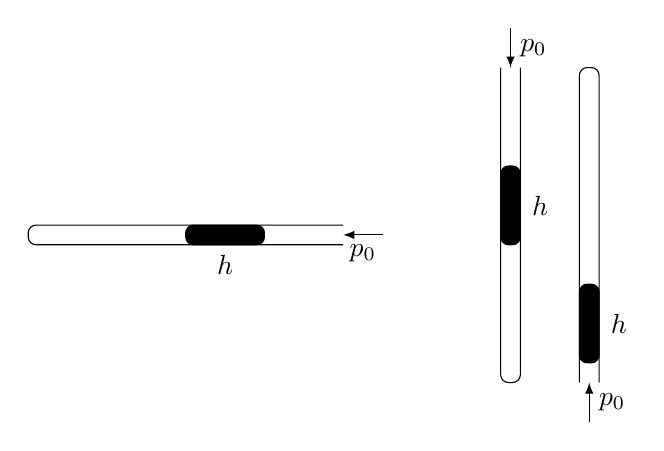
\begin{tikzpicture}[>=latex]
\draw[rounded corners=0.1cm](-2,0)--(-6,0)--(-6,-.25)--(-2,-.25);	
\draw[rounded  corners=0.1cm, fill=black](-4,-.25) rectangle (-3,0);		
\node at (-3.5,-.5){$h$};
\draw[<-](-2,-0.125)--node[below]{$p_0$}(-1.5,-.125);

\draw[rounded corners=0.1cm](0,2)--(0,-2)--(.25,-2)--(.25,2);

\draw[rounded  corners=0.1cm, fill=black](0,-.25) rectangle (.25,.75);
\node at (.5,.25){$h$};
\draw[<-](0.125,2)--node[right]{$p_0$}(0.125,2.5);


\draw[rounded corners=0.1cm](1,-2)--(1,2)--(1+.25,2)--(1+.25,-2);

\draw[rounded  corners=0.1cm, fill=black](1,-1.75) rectangle (1+.25,.75-1.5);
\node at (1.5,-1.25){$h$};
\draw[<-](1.125,-2)--node[right]{$p_0$}(1.125,-2.5);

	\end{tikzpicture}
	\caption{}
\end{figure}

温度这个物理量大家都很熟悉.温度是表示物体冷热程度的物理量,是物体分子热运动的平均动能的标志.温度的数值表示法叫做温标,我们在初中学过摄氏温标,用摄氏温标表示的温度叫做摄氏温度,在国际单位制中采用热力学温标(又常叫绝对温标),这种温标将在第四节中讨论.

研究气体的性质,首先引起我们注意的是描述气体状态的这三个物理量的变化.举例来说,地面附近的空气变热以后向空中上升时,它的体积、压强和温度都发生变化.把氧气装入钢筒时,或者用户(工厂、医院)把氧气从钢筒中放出来使用时,氧气的体积、压强和温度都发生变化.内燃机气缸里的燃料混合物爆发时,这三个物理量也都发生变化.对一定质量的气体来说,如果体积、压强和温度这三个量都不改变,我们就说气体处于一定的状态中,如果这三个物理量同时发生变化或者其中有两个发生变化,我们就说气体的状态改变了.对一定质量的气体来说,只有一个量改变而其他两个都不改变的情况,是不会发生的.那么,在气体的状态改变时,这三个物理量的变化是任意的,还是相互关联,遵循一定的规律?如果遵循一定的规律,这个规律又是什么?这就是本章讨论的中心课题.

下面,我们用实验方法先研究一定质量的气体在分别保持温度、体积不变时,其他两个量的变化规律,然后在此基础上确定三个状态参量的变化规律.


\subsection*{练习一}
\begin{enumerate}
	\item 什么叫气体的压强?举出气体对器壁有压力作用的几个实例.
	\item 大气压为750毫米汞柱时,等于多少帕?
		\item 在图3.2中,水银柱的长度为19厘米,大气压为
	760毫米汞柱,玻璃管开口向上竖直放置时,被封闭的气体的压强等于多少毫米汞柱?开口向下竖直放置时,等于多少毫米汞柱?
\begin{figure}[htp]\centering
	\includegraphics[scale=.55]{fig/3-3.png}
	\caption{}
\end{figure}


	\item 图3.3是测量气体压强的水银压强计,两端开口的U形管内装入水银,$A$管跟容器连接.已知大气压$p_0$和两管中水银面的高度差,就可以知道容器中气体的压强.大气压为$1.013\times 10^5{\rm Pa}$,图甲和图乙中的$h$都是10厘米,分别求出这两种情形中气体的压强是多少帕.
	\item 在图3.4所示的几种情形中,被封闭的气体$A$的压强分别是多少帕?大气压为$1.013\times 10^5{\rm Pa}$.
	\item 举出气体状态发生改变的几个实例.
\begin{figure}[htp]\centering
	\includegraphics[scale=.55]{fig/3-4.png}
	\caption{}
\end{figure}

\end{enumerate}

\section{气体的等温变化~~玻意耳-马略特定律}
我们先来研究温度不变时,一定质量的气体的压强随着
它的体积而变化的情形.这种变化叫做\textbf{等温变化}.
\begin{figure}[htp]\centering
	\includegraphics[scale=.55]{fig/3-5.png}
	\caption{}
\end{figure}

实验装置如图3.5所示,玻璃管$A$和$B$通过一条橡皮管连在一起,$A$管上端有一个阀门$a$,$B$管上端是开口的.$A$管固定在有刻度的竖直板上,$B$管可以上下移动,实验开始时,打开阀门$a$,从$B$管注入水银,然后关闭阀门,把一定质量的空气封闭在$A$管里.当两管中的水银面一样高时(图甲),$A$管里空气的压强等于作用在$B$管水银而上的大气压.

把$B$管慢慢提高,使$A$管里空气的体积缩小.这时$B$管里的水银面比$A$管里的高(图乙),$A$管里气体的压强等于大
气压加上$B$管水银面高出$A$管水银面的那段水银柱的压强.实验表明,在温度不变的条件下,气体的体积缩小到原来的几分之一,它的压强就增大到原来的几倍.

把$B$管慢慢放低,使$A$管里气体的体积增大,这时$B$管里的水银面比$A$管里的低(图丙),$A$管里气体的压强等于大气压减去$A$管水银面高出$B$管水银面的那段水银柱的压强.实验表明,在温度不变的条件下,气体的体积增大到原来的几倍,它的压强就减小为原来的几分之一.

改用其他气体做这个实验,得到的结果相同.

英国科学家玻意耳(1627—1691)和法国科学家马略特(1620—1684)各自独立地用实验研究了气体的压强和体积的关系,得到下面的结论:

\textbf{温度不变时,一定质量的气体的压强跟它的体积成反比}.这个结论叫做\textbf{玻意耳-马略特定律}.

玻意耳-马略特定律可以用公式来表示,保持一定质量气体的温度不变,设体积为$V_1$时压强为$p_1$,体积为$V_2$时压强为$p_2$,那么
\[\frac{p_1}{p_2}=\frac{V_2}{V_1} \]
或
\[p_1V_1=p_2V_2 \]

由此式可以看出,玻意耳-马略特定律也可以叙述为:\textbf{温度不变时,一定质量的气体的压强跟它的体积的乘积是不变的},
\[pV=\text{恒量}\]

气体的等温变化也可以用图线来表示.用直角坐标系的
横轴表示气体的体积$V$,用纵轴表示气体的压强$p$.设在一定温度下,一定质量的某种气体在$V_1=2$升时,$p_1=1$标准大气压,在图3.6中由$A$点表示.根据玻意耳-马略特定律可以
得出:$V_2=4$升时,$p_2=1/2$标准大气压,由$B$点表示;$V_3=1$升时,$p_3=2$标准大气压,由$C$点表示;$V_4=1/2$升时,$p_4=4$标准大气压,由$D$点表示.当然还可以使气体的体积等于其他许多不同的数值,并计算出相应的压强的数值,从而得到其他许多点.由这些点连成的平滑曲线,叫做气体的等温线.从等温线可以清楚地看出温度不变时气体的压强跟体积的关系.
\begin{figure}[htp]\centering
	\begin{tikzpicture}[>=stealth, domain=.45:4.5, samples=100]
\draw[<->] (0,5)node [right]{$p$(标准大气压)}--(0,0)--(5,0) node [right]{$V$(升)};

\foreach \x in {1,2,3,4}
{
   \draw (0,\x)node [left]{\x}--(.1,\x);
\draw (\x,0)node [below]{\x}--(\x,.1);
}

\draw[color=black, ultra thick] plot (\x,{2/\x}) ;

\draw [dashed] (1,0)--(1,2)--(0,2);
\draw [dashed] (2,0)--(2,1)--(0,1);
\draw [dashed] (4,0)--(4,.5)--(0,.5);
\draw [dashed] (0.5,0)--(.5,4)--(0,4);

\draw [fill=black] (1,2)node [right]{$C$}  circle (2pt);
\draw [fill=black] (2,1)node [above]{$A$}  circle (2pt);
\draw [fill=black] (4,.5)node [above]{$B$}  circle (2pt);
\draw [fill=black] (.5,4)node [right]{$D$} circle (2pt);

\node at (-.2,-.2){$0$};

\end{tikzpicture}
	\caption{气体等温变化的图线}
\end{figure}

\begin{example}
某个容器的容积是10升,所装气体的压强是$20\times 10^5$帕,如果温度保持不变,把容器的开关打开以后,容器
里剩下的气体是原来的百分之几?设大气压是$1.0\times 10^5$帕.
\end{example}

\begin{solution}
这个题目可以这样来分析.容器里装着一定质量的气体,取这一定质量的气体作为我们的研究对象.气体在初状态时,$p_1=20\times 10^5$帕,$V_1=10$升,打开开关以后,由于气体压强大于外界大气压,于是气体发生膨胀(等温膨胀),有一部分
气体跑出容器,随着气体的膨胀,气体的压强降低,最后,当气体压强等于外界大气压时,气体停止膨胀而达到末状态.这时,气体一部分在容器内,一部分在容器外.如果我们知道气体在末状态时占有多大体积,就可以知道容器里剩下的气体为原来的百分之几.

气体在初状态时,$p_1=20\times 10^5$帕,$V_1=10$升,在末状态时,$p_2=1.0\times 10^5$帕,$V_2$为待求的体积.由玻意耳-马略特定律$p_1V_1=p_2V_2$得到
\[V_2=\frac{p_1V_1}{p_2}=\frac{20\times 10^5\times 10}{1.0\times 10^5}{\rm L}=200{\rm L} \]

这时容器里剩下10升气体,所以剩下的气体是原来气体的$10{\rm L}/200{\rm L}=5\%$.
\end{solution}

从这里我们看到,利用玻意耳-马略特定律来解题,先要明确研究对象以及它的初末两个状态,然后才能利用公式来求解,用玻意耳-马略特定律解题时,还要注意等式两边的$p$或$V$必须采用相同的单位,至于具体采用什么单位,可以根据解题方便来决定.

玻意耳-马略特定律表示一定温度下气体的压强跟体积的关系,因此我们可以预料这个定律的表达式
\[pV=\text{恒量} \]
中的恒量跟温度有关系.实验表明,温度不同,这个恒量也不同,图3.7中画出了不同温度下的几条等温线,从此可以知道:一定质量的气体,保持它的体积不变,温度越高,压强越大;保持它的压强不变,温度越高,体积越大,可见,表达式中的恒量随温度而增大.这样看来,要确定体积、压强、温度这
三个物理量的变化规律,我们还需要研究压强怎样随着温度而变化或者体积怎样随着温度而变化.
\begin{figure}[htp]\centering
	\includegraphics[scale=1]{fig/3-7.pdf}
	\caption{不同温度下的几条等温线}
\end{figure}



玻意耳-马略特定律是在压强不太大(和大气压比较)、温度不太低(和室温比较)的条件下总结出来的.在这种条件下,不论什么气体都近似地符合这个定律.当压强很大、温度很低时,由这个定律得出的结果跟实际测量的结果有很大差别,这个定律就不适用了.举例来说,有一定质量的氦气,压强为1标准大气压时,体积为1${\rm m^3}$.压强为500标准大气压时,按照玻意耳-马略特定律体积应该是1/500${\rm m^3}$,而实际测量的结果是1. 36/500${\rm m^3}$,二者之间已经显示出不小的差别.压强为1000标准大气压时,按照玻意耳-马略特定律体积应该是1/1000${\rm m^3}$,而实际测量的结果是2.0685/1000${\rm m^3}$,二者相差一倍多,很本无法应用玻意耳-马略特定律了.


\subsection*{练习二}
\begin{enumerate}
		\item 把打气筒的出口堵住,往下压打气筒的活塞,会感到越往下压越费劲,怎样解释这个现象?
	\item 某个容器的容积是5升,里面所装气体的压强是10标准大气压,如果温度保持不变,把容器的开关打开以后,这些气体会有多大体积?容器里剩下的气体是原来的百分之几?设外界压强为1标准大气压.
	\item 在上题里,打开容器的开关以后,气体的密度怎样改变?设上题里容器里剩下的气体的密度是$\rho_2$,原来容器里气体的密度是$\rho_1$,那么,密度之比$\rho_2/\rho_1$是多大?
	\item 在密闭圆筒的中央有一个活塞(图3.8),活塞两边
	封闭着两部分气体,它们的压强都是750毫米汞柱,现在用
	力把活塞向右移动,使活塞右边气体的体积为原来的一半,那么活塞两边气体的压强差是多大?假定气体的温度不变.
\begin{figure}[htp]\centering
	\begin{tikzpicture}[>=latex]
\draw [pattern=north east lines](2.4,0) rectangle (2.6,2);	
  \pgfsetlinewidth{4pt}
\pgfsetinnerlinewidth{3pt}
\draw  (0,0) rectangle (5,2);
\end{tikzpicture}
\caption{}
\end{figure}

	\item 在图3.2中,水银柱的长度为19厘米,大气压为760毫米汞柱,玻璃管是粗细均匀的,玻璃管开口向上竖直放置时,被封闭的气体柱长15厘米,当开口向竖直放置时,被封闭的气体柱的长度是多少?
	\item 在下端封闭的竖直玻璃管里有一段4厘米长的水银柱,水银柱下面封闭着6${\rm cm^3}$的空气,玻璃管的横截面积是0.1${\rm cm^2}$.如果再向管里装入27.2克水银,那么,封闭在水银
 柱下面的空气柱有多高?设大气压为760毫米汞柱.
	\item 一个足球的容积是2.5升.用打气筒给这个足球打气,每打一次就把1标准大气压的空气打进去125${\rm cm^3}$,如果足球在打气前内部没有空气,打了40次以后,足球内部空气的压强有多大?假定空气的温度不变.
\end{enumerate}

\section{气体的等容变化~~查理定律}
气体在体积不变的情况下发生的变化叫做等体积变化,也叫\textbf{等容变化}.现在我们用实验来研究一定质量的气体,在体积保持不变的情况下它的压强怎样随着温度而变化.
\begin{figure}[htp]\centering
\includegraphics[scale=.6]{fig/3-9.png}
\caption{}
\end{figure}

实验装置如图3.9所示,烧瓶上连一根玻璃管,用橡皮管把它跟水银压强计连在一起,这样便在烧瓶中封入了一定质量的气体.调节压强计的可动管$A$,使两管中的水银面一样高,这时瓶里气体的压强就等于当时的大气压强(图甲),用记号标出$B$管中水银面的位置.

把烧瓶放进盛着冰水混合物的容器里,经过一段时间,瓶里气体的温度跟冰水混合物的温度一样,等于0$^\circ$C.调节压强计的$A$管,使$B$管中水银面恢复到原先标出记号的位置,也就是使气体恢复原来的体积.从压强计$B$管的水银面比$A$管的水银面高可以知道,气体压强减小了(图乙).

把烧瓶放进盛有热水的容器中,调节压强计的$A$管,使$B$管中水银面恢复到原先标出记号的位置,使气体恢复原来的体积,从压强计$B$管的水银面比$A$管的水银面低可以知道,这时气体压强增大了(图丙).

实验表明,在保持气体的体积不变的情况下,一定质量气体的压强随度的升高而增大.

1787年法国科学家查理(1746—1823)通过实验研究,发
现所有气体都遵从下述规律:

\textbf{一定质量的气体,在体积保持不变的情况下,温度每升
高(或降低)$1^\circ{\rm C}$,增加(或减小)的压强等于它在0$^\circ$C时压强的$1/273$.}这就是\textbf{查理定律}.

设一定质量的某种气体,在体积不变的条件下,0$^\circ$C时的压强为$p_0$, $t^\circ$C时的压强为$p_t$.温度升高$t^\circ$C增加的压强为$p_t-p_0$,每升高1$^\circ$C增加的压强$(p-t-p_0)/t$等于$p_0$的$1/273$,即
\[\frac{p_t-p_0}{t}=\frac{p_0}{273} \]
整理后得到
\[p_1=p_0 \left(1+\frac{t}{273}\right)\]
这就是查理定律的数学表达式.

查理定律也可以用图线来表示.用直角坐标系的横轴表示气体的温度$t$,纵轴表示气体的压强$p$.査理定律表明压强是温度的一次函数,而一次函数的图线是一条倾斜的直线,它在纵轴上的截距等于0$^\circ$C时的压强$p_0$,如图3.10所示.

查理定律也是在压强不太大、温度不太低的条件下总结出来的,在这种条件下,不论什么气体都近似地符合这个定律,当压强很大、温度很低时,每升高1$^\circ$C增加的压强不再等于$p_0$的$1/273$,而且这个数值对不同的气体也不再相同.这时查理定律就不适用了.


\section{热力学温标}
图3.10表明了气体的压强跟温度之间的关系,我们看到,图中的直线并未通过原点,说明气体的压强不是直接与摄氏温度成正比的.但是如果我们改用一个新的温标,那就可以得到压强和温度之间的简单的正比关系.

\begin{figure}[htp]\centering
	\begin{tikzpicture}[>=stealth ]
\draw[<->] (0,6.5)node [right]{$p$}--(0,1)--(6,1) node [right]{{$t^\circ$C}};

\draw[color=black, ultra thick] (0,3)--(5,6+1/3);

\draw [dashed] (1.5,+1)--(1.5,4)--(0,4);
\draw [dashed] (3,+1)--(3,5)--(0,5);
\draw [dashed] (4.5,+1)--(4.5,6)--(0,6);

\node at (-.2,-.2+1){$0$};
\node at (1.5,-.25+1){$t_1$};\node at (3,-.25+1){$t_2$};\node at (4.5,-.25+1){$t_3$};
\node at (-.25,4){$p_1$};\node at (-.25,5){$p_2$};\node at (-.25,6){$p_3$};
\node at (-.25,3){$p_0$};
\end{tikzpicture}
	\caption{气体等容变化的图线}
\end{figure}

把图3.10中的直线向左方延长,交横轴于$D$点(图3.11),$D$点表示气体的压强等于零时的温度.这个温度是多少度呢?

设$p_t=p_0 \left(1+\frac{t}{273}\right)=0$,由于$p_0\ne 0$,所以必须要求$1+\frac{t}{273}=0$,由此得出$t=-273^\circ{\rm C}$.

精确的实验证明,上节查理定律数学表达式中的273应该是273.15.这样,气体压强等于零时的温度就应该是$-273.15^\circ{\rm C}$.

\begin{figure}[htp]\centering
	\begin{tikzpicture}[>=stealth, scale=.7 ]
\draw[<->] (0,6.5)node [right]{$p$}--(0,0)--(6,0) node [right]{{$t^\circ$C}};
\draw(-6,0)--(0,0);


\draw[color=black, ultra thick] (0,2.5)--(5,5);
\draw [dashed] (0,2.5)--(-5,0);
\node at (0,-.4){$O$}; \node at (-5,-.4){$-273$};
\node at (-5,.4){$D$};
\end{tikzpicture}
	\caption{}
\end{figure}

英国科学家威廉·汤姆孙(开尔文)(1824—1907)创立了把$-273.15^\circ{\rm C}$作为零度的温标,叫做\textbf{热力学温标}(或\textbf{绝对温标}),用热力学温标表示的温度叫做\textbf{热力学温度}(或\textbf{绝对温度}).

热力学温度是国际单位制中七个基本量之一,用符号$T$表示,它的单位是开尔文,简称为开,国际符号为K.热力学温度的零度是$-273.15^\circ{\rm C}$,叫做绝对零度.就每一度的大小来说,热力学温度和摄氏温度是相同的,所以热力学温度跟摄氏温度间的关系为
\[T=t+273.15 \]
为了简化,可以粗略地取$-273^\circ{\rm C}$为绝对零度,这样就有
\[T=t+273 \]
例如,在1标准大气压下,冰的熔点为0$^\circ{\rm C}$即273K,水的沸点为100$^\circ{\rm C}$即373K.

利用热力学温标可以使查理定律的表述简化.设在体积不变的情况下,一定质量的气体温度为$t_1$时压强为$p_1$,温度为$t_2$时压强为$p_2$,那么
\[\begin{split}
p_1&=p_0\left(1+\frac{t_1}{273}\right)=p_0\frac{273+t_1}{273}\\
p_2&=p_0\left(1+\frac{t_2}{273}\right)=p_0\frac{273+t_2}{273}\\
\end{split} \]
其中$p_0$表示0$^\circ$C时的压强.把上面两式相除得到
\[\frac{p_1}{p_2}=\frac{273+t_1}{273+t_2} \]
用热力学温度$T_1$和$T_2$分别代换$(273+t_1)$和$(273+t_2)$,得到
\[\frac{p_1}{p_2}=\frac{T_1}{T_2} \]
可见查理定律可以表述为:\textbf{体积不变时,一定质量的气体的压强跟热力学温度成正比}.

上面是把查理定律“外推”到零压强而引入热力学温标的,这种“外推”是可以理解的.随着温度的降低,气体分子热运动减弱,分子对器壁的撞击作用也减弱,因而压强减小.由此推想,在某一个温度下,气体压强变为零,这个温度就是绝对零度.实际上,在达到绝对零度之前,任何气体都已液化甚至变为固体,查理定律早已不适用了.虽然如此,由“外推”得到的绝对零度仍具有物理意义,它是低温的极限,能够无限接近,但不可能达到.

\subsection*{练习三}

\begin{enumerate}
	\item 炎热的夏天,打足了气的自行车胎在日光曝晒下有时会胀破,解释这个现象.
\item 乒乓球挤瘪后,放在热水里泡一会,会重新鼓起来.解释这个现象.
\item 一定质量的氢气在0$^\circ$C时的压强是700毫来汞柱,它在30$^\circ$C时的压强是多大?压强为650毫米汞柱时它的温度
是多少摄氏度?保持氢的体积不变.
\item 一定质量的某种气体,在20$^\circ$C时的压强是$1.0\times 10^5$帕,如果保持它的体积不变,温度升高到50$^\circ$C时,它的压强是多大?温度降低到$-7^\circ$C时,它的压强又是多大?
\item 盛有氧气的钢筒,在室内(室温是17$^\circ$C)测得筒内气体的压强是$9.31\times 10^8$帕,当钢筒搬到温度是$-$13$^\circ$C的工地时,筒内气体的压强变为$8.15\times 10^8$帕.钢筒是不是漏了气?为什么?
\item 装在容器中的气体,体积为4升,压强为$2.0\times 10^5$帕,温度为300开,先让气体发生等容变化,压强增大为原来的2倍,然后让气体发生等温变化,压强又降低到原来的数值.求气体在末状态时的体积和温度.

\end{enumerate}

\section{理想气体的状态方程}
前面我们研究了一定质量的气体在温度不变时压强跟体积的关系以及体积不变时压强跟温度的关系,分别得出了玻意耳-马略特定律和查理定律.现在我们从这两个实验定律出发,确定一定质量的气体的体积、压强、温度这三个状态参量在变化中的相互关系.

设有一定质量的气体,在初状态时的压强、体积和温度分别为$p_1,V_1,T_1$,经过某个变化过程,到末状态时这三个量分别变成$p_2,V_2,T_2$.气体从初状态到末状态可以经过各种不同的变化过程,现在设想有一个变化过程是分两个阶段进行的.在第一个阶段中,保持温度$T_1$不变,体积从$V_1$变成$V_2$,压强从$p_1$变成另一个值$p_2$(图3.12中的1和2).在第二个阶段
中,保持体积$V_2$不变,温度从$T_1$变成$T_2$,压强从$p_c$变成$p_2$(图3.12中的2和3).

\begin{figure}[htp]\centering
	\begin{tikzpicture}[>=stealth, xscale=2, yscale=.8 ]
\draw [rounded corners=0.2cm, very thick](-3,2)--(-3,-2)--(-1.5,-2)--(-1.5,2);
\draw [pattern=north east lines](-3,0) rectangle (-1.5,0.5);	
\node at (-4.5/2, -1){$p_1\quad V_1\quad T_1$};
\node at (-4.5/2, -2.5){1};
\draw[->](-1.4,0)--node [above]{等温}(-.6,0);



\draw [rounded corners=0.2cm, very thick](-.5,2)--(-.5,-2)--(1,-2)--(1,2);
\draw [pattern=north east lines](-.5,-1) rectangle (1,-0.5);	
\node at (.5/2, -1.5){$p_c\quad V_2\quad T_1$};
\draw [fill=gray!30](0.2,-.5) rectangle(0.4,.5);
\node at (.5/2, -2.5){2};
\draw[->](1.1,0)--node [above]{等容}(1.9,0);

\draw [rounded corners=0.2cm, very thick](2,2)--(2,-2)--(3.5,-2)--(3.5,2);
\draw [pattern=north east lines](2,-1) rectangle (3.5,-0.5);
\draw [fill=gray!30](2.5,-.5) rectangle(2.7,.5);
\draw [fill=gray!30](2.9,-.5) rectangle(3.1,.5);	
\node at (5.5/2, -1.5){$p_2\quad V_2\quad T_2$};
\node at (5.5/2, -2.5){3};


\end{tikzpicture}
	\caption{}
\end{figure}

第一个阶段是等温变化,根据玻意耳-马略特定律有
\begin{equation}
p_1V_1=p_2V_2
\end{equation}
第一个阶段是等容变化,根据查理定律有
\begin{equation}
\frac{p_c}{T_1}=\frac{p_2}{T_2}
\end{equation}
由(3.1)式解出$p_c$,代入(3.2)式,整理后得到
\begin{equation}
\frac{p_1V_1}{T_1}=\frac{p_2V_2}{T_2}
\end{equation}

上式说明,一定质量的气体从初状态$(p_1,V_1,T_1)$变到末状态$(p_2,V_2,T_2)$,压强和体积的乘积与热力学温度的比值是不变的,即
\begin{equation}
\frac{pV}{T}=\text{恒量}
\end{equation}

我们知道,玻意耳-马略特定律和查理定律是在压强不太大、温度不太低的条件下总结出来的.在这种条件下,不论什么气体都近似地符合这两个实验定律.(3.4)式是从上述两个实验定律推导出来的,因此,也只有在这种条件下,不论什么

气体才近似地符合(3.4)式.尽管如此,为了研究的方便,我们还是可以设想出一种气体,能够在任何温度和压强下都遵守(3.4)式,这样的气体叫做\textbf{理想气体}.(3.4)式叫做一定质量的理想气体的状态方程.

当然,理想气体是不存在的,它只是实际气体在一定程度上的近似.有许多实际气体,特别是那些不易液化的气体,如氢气、氧气、氮气、空气、氦气等,在通常的温度和压强下,它们的性质很近似于理想气体,可以把它们当作理想气体来处理.这样处理的结果,误差很小,可是计算起来却简便多了.

理想气体状态方程实际上包含了前面讲的两个气体实验
定律,如果保持温度$T$不变,便得到$pV=\text{恒量}$,这就是玻意耳-马略特定律.如果保持体积$V$不变,便得到$p/T=\text{恒量}$,这就是查理定律.

从理想气体状态方程还可以知道,压强保持不变时,一定质量气体的体积怎样随着温度而变化,这种变化叫做\textbf{等压变化}.在保持压强$p$不变时,得到$V/T=\text{恒量}$,这表示\textbf{压强不变时,一定质量气体的体积跟热力学温度成正比}.这个关系最初是法国科学家盖·吕萨克(1778—1850)研究气体热膨胀时得到的实验定律,叫做\textbf{盖·吕萨克定律}.在压强不太大、温度不太低时,不论什么气体都近似地符合这个定律.


\subsection*{练习四}

\begin{enumerate}
	\item 对一定质量的气体来说,能否做到:
	\begin{enumerate}
	\item	保持压强和温度不变而改变它的体积?
	\item	保持温度和体积不变而改变它的压强?
	\item	保持体积和压强不变而改变它的温度?	 
	\end{enumerate}
\item  对一定质量的气体来说,能否做到:
\begin{enumerate}
\item 保持压强不变,同时升高温度并减小体积?
\item 保持温度不变,同时增加体积并减小压强?
\item 保持体积不变,同时增加压强并降低温度?
\end{enumerate}

\item  一定质量的空气,27$^\circ$C时的体积为$1.0\times 10^{-2}{\rm m}^3$.计算在压强不变的情况下,温度升高到100$^\circ$C时的体积.
\item  某种柴油机的气缸容积为$0.83\times 10^{-3}{\rm m^3}$.压缩前其中空气的温度为47$^\circ$C,压强为$0.8\times 10^5$帕,在压缩冲程,活塞把空气压缩到原体积的1/17,压强增大到$40\times 10^5$帕.求这时空气的温度.
\item  在容积为25升的容器中,盛有温度为37$^\circ$C、压强为62标准大气压的氧气.求氧气在标准状态(0$^\circ$C,1标准大气压)下的体积,从化学课中学过,在标准状态下,1摩的任何气体的体积都是22.4升.你能不能由此求得容器中氧气的摩尔数并进而求得氧气的质量?怎样求?
\item  一个瓶子里装有某种气体,瓶上有一个小孔跟外面大气相通.原来瓶里气体的温度为15$^\circ$C.如果把它加热到207$^\circ$C,瓶里保留的气体的质量是原来质量的几分之几?
\item  贮气筒内装有压缩气体,温度是27$^\circ$C,压强是$40\times 10^5$帕,如果从筒内放出一半质量的气体,并使筒内剩余的气体的温度降到12$^\circ$C,这些剩余气体的压强是多大?

\end{enumerate}


\section{克拉珀龙方程}
\subsection{摩尔气体恒量} 

上一节讲的气体状态方程
\[\frac{pV}{T}=\text{恒量} \]
是一定质量的理想气体状态方程,其中的恒量跟气体的质量有关系.在体积和温度相同的情况下,气体的质量越多,气体的压强就越大,因而上式中的恒量就越大.自行车车胎里打进的空气越多,车胎胀得越硬,这是大家都知道的.

实验表明,上式中的恒量还跟气体的种类有关系.在体积和温度相同的情况下,质量相同的不同种类气体,它们的压强并不相同,因而上式中的恒量也不相同.

那么,怎样在一般情况下应用上式呢?我们先把上式用于质量限定的各种气体,而且质量就限定为1摩尔.这是因为,在标准状态下,即$p_0=1$标准大气压,$T_0=273$开,1摩的任何气体的体积都是$V_0=22.4$升.由此我们可以求得一个适用于1摩尔任何气体的恒量,叫做\textbf{摩尔气体恒量},它通常用$R$来表示,即
\[R_0=\frac{p_0V_0}{T_0} \]

$R$的数值跟$p,V,T$的单位有关.在国际单位制中,$p_0=
1.013\times 10^5{\rm Pa}=1.013\times 10^5{\rm N}/{\rm m^2}$,$V_0=22. 4\times 10^{-3}{\rm m^3}/{\rm mol}$,$T_0=273{\rm K}$,代入上式得到
\[\begin{split}
R&=\frac{1.013\times 10^5{\rm N}/{\rm m^2}\times  22. 4\times 10^{-3}{\rm m^3}/{\rm mol}}{273{\rm K} }\\
&=8.31{\rm J}/({\rm mol\cdot K})
\end{split} \]

对于1摩的理想气体,因为$pV/T=p_0V_0/T_0=R$,所以
$$pV=RT$$
这就是1摩的理想气体的状态方程,它对任何气体都适用.

摩尔气体恒量是热学中又一个重要常数,不仅在研究气
体的热学性质中,而且在研究其他热现象中,它与阿伏伽德罗常数共同起着重要作用.

\subsection{克拉珀龙方程} 

知道了1摩的理想气体的状态方程,我们不难得到任意质量的理想气体的状态方程.设有质量为$m$千克的某种理想气体,它的摩尔质量为$M$千克/摩,它的摩尔数$n=m/M$摩.既然1摩的理想气体在标准状态下占有体积$V_0$($=22.4$升),那么$n$摩的理想气体在标准状态下占有的体积应为$V'_0=nV_0$.由理想气体的状态方程可得:
\[\begin{split}
\frac{pV}{T}&=\frac{p_0V'_0}{T_0}\\
&=n\frac{p_0V_0}{T_0}=nR
\end{split} \]
由此得到
\[pV=nRT \]
或\[pV=\frac{m}{M}RT \]
这就是任意质量的理想气体的状态方程,又叫做\textbf{克拉珀龙方程}.只要温度不太低,压强不太大,这个方程对一切气体都适用,这个方程在实际中有广泛的应用,可以用来解决有关气体的各种问题.

\begin{example}
容积为30升的瓶内装有氢气.假定在气焊过程中,温度保持27$^\circ$C不变,当瓶内压强由$4. 9\times 10^6$帕降为$9.8\times 10^5$帕时,共用去多少氢气?
\end{example}

\begin{solution}
用国际单位制来计算,把已知各个量的数值用相应的单位表示出来.
$p_1=4.9\times 10^6{\rm Pa}$;$V=30{\rm L}=30\times 10^{-3}{\rm m^3}$; $p_2=9.8\times 10^5{\rm Pa}$;$T=(27+273){\rm K}=300{\rm K}$;$M=2\times 10^{-3}{\rm kg}/{\rm mol}$.

这个例题可以这样来解:根据克拉珀龙方程先计算瓶内原有氢气的质量$m_1$,再计算气体状态改变后瓶内氢气的质量$m_2$,二者之差$m_1-m_2$就是用去的氢气的质量.

气体的初状态和末状态的体积$V$和温度$T$保持不变,压强$p$和质量$m$发生了变化,压强由$p_1$变到$p_2$,质量由$m_1$变到$m_2$.

由$p_1V=\dfrac{m_1}{M}RT$ 得到 $m_1=\dfrac{p_1VM}{RT}$
;
由$p_2V=\dfrac{m_2}{M}RT$ 得到 $m_2=\dfrac{p_2VM}{RT}$
.
所以
\[m_1-m_2=\frac{VM}{RT}(p_1-p_2) \]
代入数值得到
\[\begin{split}
m_1-m_2&=\frac{30\times 10^{-3}\times 2\times 10^{-3}}{8.31\times 300}(4.9\times 10^6-9.8\times 10^5){\rm kg}\\
	&=9.4\times 10^{-2}{\rm kg}
\end{split} \]
\end{solution}

如果就一定质量的气体来考虑气体的状态变化,即压强由$p_1$降低到$p_2$,而体积由$V_1$膨胀到$V_2$,能不能解出这个题目?你来试一下,并把两种解法加以比较.

利用理想气体状态方程解题,首先要明确我们所研究的对象是哪部分气体,以及气体状态发生变化时它的初状态和末状态,然后才能用状态方程来求解,计算时要注意物理量的单位,$T$必须采用热力学温度,根据$p_1V_1/T_1=p_2V_2/T_2$解题时,公式两边的$p$和$V$的单位必须统一,根据$pV=mRT/M$解题时,$R$的单位必须与$p$、$V$的单位相适应.

\subsection*{练习五}

\begin{enumerate}
	\item 如果压强用标准大气压作单位,体积用升作单位,试通过计算证明:$R=0.082$标准大气压·升/(摩·开).
\item 一个容器内装有氧气100克,压强为10标准大气压,温度为47$^\circ$C,容器的容积是多少${\rm m^3}$?
\item 1克的气体,温度为27$^\circ$C、压强为600毫米汞柱时,体积为5升,2克的同种气体,温度为127$^\circ$C、压强为400毫米汞柱时,体积是多少升?
\item 容积是10升的钢筒里盛有90标准大气压、$-13^\circ$C的氧气,求钢筒中氧气的质量.已知氧气在标准状态下的密度$\rho_0=1.43{\rm kg}/{\rm m^3}$.
\item 有0.612克的某种氮氧化合物,在293开和1标准大气压时体积为480${\rm cm^3}$,这是一种什么气体?写出它的分子式.
\item 给汽车轮胎打气,使胎内空气达到所需的压强,冬天和夏天打入胎内的空气质量是否相同?冬天还是夏天打入的空气质量多?
\item 有两种不同种类的气体,它们的温度和体积都相同.如果它们的质量也相同,气体的压强是否相同?如果它们的质
量不同,但摩尔数相同,气体的压强是否相同?
\item 理想气体的状态方程可写成$pV/T=C$(恒量),对于这个恒量$C$,下面哪种说法正确,哪种说法错误,并说明理由.
\begin{enumerate}
\item 对质量相同的任何气体,$C$都相同.\item 对质量不同的同种气体,$C$都相同.	\item 对摩尔数不同的同种气体,$C$都相同.\item 对摩尔数相同的任何气体,$C$都相同.
\end{enumerate}
\end{enumerate}

\section{气体分子运动的特点}
\subsection{分子间的距离较大} 
气体很容易被压缩,说明气体分子间的距离比较大,气体凝结成液体时,体积要缩小上千倍,而液体不容易被压缩,可以认为其中的分子几乎是紧密排列的,可见气体分子之间的距离大约是分子直径的$\sqrt[3]{1000}$倍,即10倍.由于气体分子间的距离比较大,所以在处理某些问题时可以把气体分子看作是没有大小的质点.也是由于气体分子间的距离比较大,分子间的相互作用力十分微弱,所以通常可以认为,气体分子除了相互碰撞或者跟器壁碰撞外不受力的作用,可以在空间里自由移动.由此可以说明:气体能充满它所能达到的空间,既没有一定的体积,没有一定的形状.

\subsection{分子间的碰撞频繁} 
比起固体和液体来,气体中的分子是比较稀疏的,但是单位体积中的分子数还相当大.在标准状态下,1${\rm cm^3}$气体中仍含有$2.7\times 10^{10}$个分子,大量分子永不停息地运动,分子之间不断地发生碰撞,在标准状态下,一个空气分子在1秒内与其他空气分子的碰撞竞达65亿次之多.频繁的碰撞使得每个分子的速度的大小和方向频繁地改 
变.设想我们追随某个气体分子的运动(图3.13),我们将看到这个分子的运动是忽左忽右,忽前忽后,时快时慢,运动轨迹是一条极不规则的折线,频繁的碰撞造成气体分子做杂乱无章的热运动.
\begin{figure}[htp]\centering
\includegraphics[scale=.6]{fig/3-13.png}
\caption{}
\end{figure}

通常假定分子之间或分子与器壁之间的碰撞是完全弹性碰撞.

\subsection{分子沿各方向运动的机会均等} 

气体分子做杂乱无章的热运动,就某一个分子来说,它在某一时刻的速度具有怎样的大小和方向,完全是偶然的.但是,对大量分子的整体来说,分子的运动却表现出一定的规律,先来讨论分子运动的方向.正因为大量分子的运动十分混乱,在某一时刻向任一方向运动的分子都有,因而可以想见,在任一时刻分子沿各方向运动的机会是均等的,没有任何一个方向,沿着它运动的分子的数目更多,设想真有这么一个方向,那么,由于气体分子的频繁碰撞,分子的运动越来越混乱,这个方向也不会存在了,这就是说,气体分子沿各个方向运动的数目应该是相等的.

这里所说的数目相等,是对大量分子用统计方法得到的一个统计平均数,与实际数目会有微小的出入,分子数越多,这种用统计方法得到的结果跟实际情况越符合,用分子运动论的观点研究热现象,涉及的总是大量分子,统计方法非常有用.

\subsection{分子速率按一定规律分布} 
大量分子做无规则运动,速率有的大,有的小,但分子的速率却按照一定的规律分布.

研究表明,气体的大多数分子,速率都在某个数值附近,离开这个数值越远,分子数越少,表现出“中间多,两头少”的
分布规律,下表是氧气分子速率的分布情况.我们看到,在0$^\circ$C时速率在300—400$\ms$这一速率区间的分子数最多,速率大于400$\ms$和小于300$\ms$的分子数依次递减,速率很大和很小的分子实际上很少,温度升高时,这种“中间多,两头少”的分布规律虽然不变,可是与分子数的最大值相对应的速率区间却移向速率大的一方,也就是说,温度升高时,速率小的分子数减少,速率大的分子数增加,这种速率分布规律是一种统计规律,表中的在某一速率区间的相对分子数,也是
对大量分子用统计方法得到的统计平均数,与实际数值会有微小的出入.

\begin{table}
	\centering\caption{氧气分子的速率分布}
	\begin{tabular}{ccc}
\hline
按速率大小划分的区间 & \multicolumn{2}{c}{各速率区间的分子数占总分子数的百分率}\\
($\ms$)& 0$^\circ $C & 100$^\circ $C\\
\hline
100以下 & 1.4 & 0.7\\
100—200 &	8.11 &	5.4
\\
200—300 &	7.0	 &11.9
\\
300—400 &	21.4 &	17.4
\\
400—500 &	20.4 &	18.6
\\
500—600 &	15.1 &	16.7
\\
600—700 &	9.2 &	12.9
\\
700—800  &	4.5 &	7.9
\\
800—900 &	2.0 &	4.6
\\
900 以上 &	0.9 &	3.9\\
\hline
	\end{tabular}
\end{table}

既然在一定温度下,某种气体的分子速率分布是确定的,我们就可以求出在这个温度下该种气体分子的平均速率,即所有分子的速率的平均值.温度升高时,速率大的分子数增
加,分子的平均速率增大.例如氮气分子的平均速率在$-150^\circ $C时为320$\ms$,在$0^\circ $C时为493$\ms$,在$1000^\circ $C时
为1194$\ms$.这里我们又一次看到,温度越高,分子的热运动越激烈.

\section{气体实验定律的微观解释}
\subsection{气体压强的微观解释} 
从气体分子运动论的观点看来,气体压强是大量的气体分子频繁地碰撞器壁而产生的.雨滴打在雨伞上,使伞面受到冲力,单个雨滴对伞面的冲力是短暂的,但大量密集的雨滴接连不断地打在伞面上,对伞面就形成一个持续的均匀的压力,同样,单个分子碰撞器壁的冲力是短暂的,但是大量分子频繁地碰撞器壁,就对器壁产生持续的均匀的压力,下面我们从气体分子运动论的观点定性地讨论一下气体的压强.

设想容器内只有一个分子,我们可以利用以前学过的力学知识算出这个分子碰撞器壁时对器壁产生多大的冲力,现在的问题是:容器中有大量分子,它们的速度的大小和方向又不断地在改变.怎样才能算出大量分子碰撞器壁时对器壁产生的冲力呢?

我们知道,气体分子做无规则运动,它们沿各个方向运动的机会是均等的,也就是说,在上下、前后、左右各个方向中没有哪个方向的运动占优势,因此我们可以认为各有1/6的分子向着上下前后左右这六个方向运动,气体分子速度的大小也不相同,但我们可以认为所有分子都以平均速率向着各个
方向运动.

\begin{figure}[htp]\centering
	\begin{tikzpicture}[>=stealth, scale=.9 ]
\draw (5,2)--(5,-2);
\fill [pattern=north east lines](5,-2) rectangle(5.25,2);

\draw [shade](0,0) circle (4mm);
\draw [dashed] (3.5,0) circle (4mm);
\draw[->](0,0)--(1,0) node [above]{$v$};
\draw[->](3.5,0)--(2.5,0)node [above]{$v'=v$};


\end{tikzpicture}
	\caption{气体分子每碰撞一
次器壁,就给器壁$2mv$的冲量.}
\end{figure}



现在设想有一个向右运动的分子与器壁发生碰撞(图3.14),碰撞前的动量是$mv$,其中$v$是分子的平均速率,碰撞后向左运动,速率是$v'$,动量是$-mv'$.这个分子碰撞前后的动量变化是$-mv'-mv$.气体分子与器壁之间的碰撞是完全弹性碰撞,这样,分子碰撞前后的速率相等,即$v'=v$,因而动量变化是$-2mv$.从动量定理知道,这个动量变化$-2mv$等于器壁对分子的冲量.从牛顿第三定律知道,这时分子对器壁也有一个大小相等方向相反的冲量.可见气体分子每碰撞一次器壁,就给器壁$2mv$的冲量.

在一段时间内,大量分子与器壁碰撞多少次,分子给器壁
的总冲量就是$2mv$的多少倍,而在单位时间内分子给器壁的总冲量就等于器壁所受的压力,单位面积器壁所受的压力就等于气体的压强.

这样,如果知道单位时间内分子对单位面积器壁的碰撞次数,就可以求得气体的压强.这个碰撞次数跟单位体积内气体的分子数有关,单位体积内气体的分子数越多,即气体分子越密,这个碰撞次数就越多,这是容易理解的.这个碰
撞次数还跟分子的平均速率有关.如图3.15所示,我们在气体内部设想一个柱体,底面积为单位面积,高为平均速率的数值.在单位时间内,这个柱体中向右运动的分子都会运动到器壁而发生碰撞.平均速率越大,这个柱体越高,其中的分子越多,分子与器壁发生碰撞的次数就越多.可见,单位时间内分子对单位面积器壁的碰撞次数是由单位体积内的分子数和分子的平均速率决定的.由此我们将不难理解气体压强也是由单位体积内的分子数和分子的平均速率决定的,单位体积内的分子数越多,分子的平均速率越大,气体的压强就越大.
\begin{figure}[htp]\centering
	\begin{tikzpicture}[>=stealth, scale=.9 ]
\draw (5,2)--(5,-2);
\fill [pattern=north east lines](5,-2) rectangle(5.25,2);

\draw[dashed, pattern=crosshatch dots](1,-.3) rectangle (5,.3);
\draw(1,-.3)--(1,-1);
\draw[<->](1,-.65)--node [below]{$v$}(5,-.65);

\end{tikzpicture}
	\caption{单位时间内分子对单位
面积器壁的碰撞次数跟
分子的平均速率有关.}
\end{figure}

\subsection{气体实验定律的微观解释} 
知道了气体压强是由什么决定的,我们就能够用气体分子运动论对气体实验定律作出微观解释.

一定质量的气体,温度保持不变,也就是分子的总数和分
子的平均速率保持不变.在这种情况下,气体的体积减小到原来体积的几分之一,单位体积内的分子数就增大到原来的几倍,气体的压强就增大到几倍,气体体积增大时,情况恰好相反,结果是气体的压强与体积成反比,这就是玻意耳-马略特定律.

用气体分子运动论也可以解释查理定律,一定质量的气体,体积保持不变而温度升高时,分子的平均速率增大,因而气体的压强增大,温度降低时,情况恰好相反.

怎样解释盖·吕萨克定律呢?从气体分子运动论可以说明:一定质量的气体温度升高时,要保持压强不变,只有让气体的体积增大才行.这时,一方面由于温度升高,分子的平均速率增大,以致每次碰撞给器壁的冲量增加,同时单位时
间内对单位面积器壁的碰撞次数增多,使压强有增大的倾向;另一方面,由于体积增大,单位体积内的分子数减少,以致单位时间内分子对单位面积器壁的碰撞次数减少,使压强有减小的倾向,当体积增大到一定程度时,这两种倾向抵消,所以压强保持不变.

气体分子运动论不仅能够解释上述气体实验定律,而且能够解释气体的其他一些性质,如气体的比热、扩散、热传导等,气体分子运动论是热学和分子物理学的重要组成部分,它使人们对气体的研究从宏观领域进入微观领域,扩展和加深了人们对气体性质的认识.


\subsection*{练习六}

\begin{enumerate}
	\item 现在我们用另一种方法估算一下气体分子间的距离与分子直径的关系.在标准状态下,1摩的气体占有22.4升的体积.我们设想其中的每个分子都位于一个小立方体的中心.这个小立方体的边长是多少?分子直径的数量级为$10^{-10}$米.把小立方体的边长跟分子直径相比较,结果怎样?
\item 根据第七节表中的数据能不能估算出0$^\circ$C和100$^\circ$C时氧气分子的平均速率?怎样估算?结果怎样?
\end{enumerate}

\section{理想气体的内能}
从气体分子运动论的观点看来,所谓理想气体,是指分子间没有相互作用和分子可以看成没有大小的质点的气体.这就是理想气体的微观模型,一定质量的气体,温度越高,压强
越小,因而气体越稀薄,气体分子间的距离越大,就越接近于理想气体.在温度较低和压强较大的情况下,气体不那么稀薄,在研究气体的性质时必须考虑到分子的大小和分子间的相互作用,而它们跟气体的种类有关,这时气体不再遵守理想气体状态方程,并且显示出不同气体在性质上的差异.

理想气体的分子之间既然没有相互作用,就不存在分子势能,因此,理想气体的内能就是气体所有分子热运动的动能的总合,分子的动能跟气体的温度有关,分子势能跟气体的体积有关,现在不存在分子势能,因而理想气体的内能只跟温度有关,跟体积无关.这就是说,只要温度保持不变,气体的体积增大一些因而气体分子疏一些,或者气体的体积减小一些因而气体分子密一些,不仅分子动能保持不变,分子势能仍旧不存在,因此理想气体的内能保持不变.

\section{理想气体的内能变化}
前面我们讲过了理想气体的等温、等容和等压变化,现在我们分析一下在这三种等值变化中内能的变化.

设一定质量的理想气体在温度不变的情况下发生膨胀,由初状态变到末状态,由于温度保持不变,所以气体的内能也不变,即$\Delta E=0$.气体发生膨胀时对外做功,所以$W$为负值,即$W<0$.从热力学第一定律$W+Q=\Delta E=0$知道,$Q$应为正值,即$Q>0$,而且$W$和$Q$的绝对值相等.可见,在等温膨胀的过程中,理想气体要从外界吸收热量,吸收的热量并没有增加气体的内能,而全部用来对外做功.

在体积不变的情况下,对一定质量的理想气体加热,使它的温度升高,压强增大,由初状态变到末状态.末状态的温度比初状态高,所以内能增加,即$\Delta E>0$.气体的体积不变,外界既没有对气体做功,气体也没有对外界做功,所以$W=0$.根据热力学第一定律我们得到$Q=\Delta E$.可见,在等容变化中,如果理想气体从外界吸收热量,这个热量就全部用来增加气体的内能.

在压强不变的情况下,对一定质量的理想气体加热,使它的温度升高,体积增大,由初状态变到末状态,末状态的温度比初状态高,所以内能增加,即$\Delta E>0$,气体膨胀对外做功,$W<0$.从热力学第一定律$W+Q=\Delta E>0$知道,这时气体吸收的热量$Q$的绝对值大于$W$的绝对值,这就是说,在等压膨胀的过程中,理想气体从外界吸收的热量,一部分用来增加气体的内能,一部分用来对外做功.

除了上述三种等值变化外,还有一种所谓绝热变化在实际中常常遇到,物体在状态的变化过程中如果跟外界没有热交换,这种变化就叫做\textbf{绝热变化},绝热变化的特点是:$Q=0$.用绝热良好的材料把容器包起来,让气体发生膨胀或者对气体进行压缩,这时的变化就可以看作绝热变化,气体的膨胀或压缩进行得很迅速,从初状态到末状态所用的时间很短,气体来不及跟外界发生热交换,这种迅速的变化也可以看作绝热变化,图2.1所示的压缩气体的演示,热机气缸内气体膨胀做功,过程进行得很迅速,都可以看作绝热变化.在绝热压缩的过程中,外界对气体所做的功完全用来增加气体的内能,使气体的温度升高.在绝热膨胀的过程中,气体对外界做功
完全靠气体内能的减少,因而气体的温度降低.


\subsection*{练习七}
\begin{enumerate}
	\item 一定质量的理想气体在温度不变的情况下被压缩,气体的内能是否改变?外界对气体是否做功?气体从外界吸热还是向外界放热?功和热量有什么关系?
\item 一定质量的理想气体在体积不变的情况下压强减小,这时外界对气体是否做功?气体的内能是否改变,怎样改变?气体放出的热量跟内能的改变有什么关系?
\item 一定质量的理想气体在压强不变的情况下体积减小,外界对气体是否做功?气体的内能是否改变,怎样改变?气体放热还是吸热?这个热量跟内能的改变有什么关系?
\end{enumerate}

\section*{习题}
\begin{enumerate}
	\item 下面几种说法,哪个正确,哪个错误,并说明理由.
	\begin{enumerate}
		\item 有两个相同的容器,内装同种气体,它们的压强相同,因而它们的温度一定相同.
		\item 有两个相同的容器,内装质量相同的不同气体,它们的压强不同,因而它们的温度一定不同.
		\item 有两个相同的容器,内装摩尔数相同的气体,它们的压强相同,因而它们的温度一定相同.
	\end{enumerate}
\item 一定质量的理想气体,处在某一初始状态,现在要使气体的温度经过状态变化后回到初始状态的温度,用下列哪些过程可能实现?
\begin{enumerate}
	\item 先保持压强不变而使它的体积膨胀,接着保持体积不变而减小压强.
\item 先保持压强不变而使它的体积减小,接着保持体积不变而减小压强.
\item 先保持体积不变而增大压强,接着保持压强不变而使它的体积膨胀.
\item 先保持体积不变而减小压强,接着保持压强不变而使它的体积膨胀.	 
\end{enumerate}
\item 盖·吕萨克定律如果用摄氏温标$t$来表示,可以写成下式:
\[V_t=V_0\left(1+\frac{t}{273}\right) \]
其中$V_0$和$V_t$分别表示气体在0$^\circ$C和t$^\circ$C时的体积.试推导出上式.
\item 能不能根据玻意耳-马略特定律和盖·吕萨克定律推出一定质量的理想气体的状态方程$PV/T=$恒量?实际推导一下.
\item 当温度为27$^\circ$C、压强为$2.0\times 10^5$帕时,32克氧气的体积是多大?密度是多大?另有48克氧气,温度和压强跟上述数值相同,氧气的密度又是多大?	
\item   试根据克拉珀龙方程推导出用压强和温度来表示的气体密度的表达式.
\item  水银气压计中混入了一个空气泡,上升到水银柱的上方,使水银柱上方不再是真空,因而气压计的读数比实际的大气压小些,当实际大气压为768毫米汞柱时,气压计的读数只有750毫米汞柱,此时管中水银面到管顶的距离为80毫米,当气压计读数为740毫米汞柱时,实际大气压为多少?设温度保持不变.
\item  在湖面下50米深处(温度为4$^\circ$C)有一个体积为10
${\rm cm^3}$的气泡升到湖面上来,湖面的温度为17$^\circ$C,求它升到湖面时的体积,大气压强为$1.013\times 10^5$帕.
\item  有两个容积相等的器,里面盛有同种气体,用一段水平玻璃管把它们连结起来.在玻璃管的正中央有一段水银柱,当一个容器中气体的温度是0$^\circ$C,另一个容器中气体的温度是20$^\circ$C时,水银柱保持静止,如果使两容器中气体的温度都升高10$^\circ$C,管中的水银柱会不会移动?如果移动的话,向哪个方向移动?试根据学过的气体定律加以说明.
\item  一个容器,如果其中气体十分稀薄,通常就说这个容器为“真空”.有一个容积为10${\rm cm^3}$的电子管,在温度为300开时用真空泵把它抽成真空,使管内气体压强为 $5\times 10^{-8}$毫米汞柱,这时管内有多少个气体分子?
\item  氧气瓶的容积是32升,其中氧气的压强是130标准大气压.规定瓶内氧气压强降到10标准大气压时就要重新充氧.有一个车间,每天需用1标准大气压的氧气400升.这瓶氧气能用几天?假定温度保持不变.
\begin{figure}[htp]\centering
	\begin{tikzpicture}[>=stealth, scale=.7 ]


\draw[very thick] (-2, -1.5)--(2, -1.5);
\draw[very thick] (-2, 1.5)--(2, 1.5);
\draw[very thick] (2,.2)--(5,.2); \draw[very thick] (2,-.2)--(5,-.2);
\draw[very thick] (5, 2.5)--(10, 2.5); \draw[very thick] (5, -2.5)--(10, -2.5);
\draw[very thick] (-2, 1.5)--(-2, -1.5);
\draw[very thick] (2, 1.5)--(2, .2);
\draw[very thick] (2, -.2)--(2, -1.5);
\draw[very thick] (5, 2.5)--(5, .2);
\draw[very thick] (5, -.2)--(5, -2.5);
\draw[dashed](-3,-2.5) rectangle (3,2.5);

\fill [pattern=north east lines, draw](8,-2.5) rectangle(8.5,2.5);
\node at (0,2){127$^\circ$C}; \node at (9,2){$D$}; 
\node at (0,0){$B$};  \node at (7,0){$A$};

\draw [->](10,0)node [below]{$p_0$}--(8.5,0);

\draw(3.5,-.5)--(3.5,.5);
\draw(3.2,.5)--(3.7,.5)node[right]{$K$};

\end{tikzpicture}
\caption{}
\end{figure}


\item  如图3.16所示,气缸$A$和容器$B$由一细管经阀门
$K$相联.$A$和$B$的壁都是透热的.$A$放在27$^\circ$C、1标准大气压的大气中,$B$浸在127$^\circ$C的恒温槽内.开始时$K$是关断的,
$B$内没有气体,容积$V_B=2.4$升;$A$内装有气体,体积$V_A=
4.8$升.打开$K$,使气体由$A$流入$B$,等到活塞$D$停止移动
时,$A$内气体的体积是多大?假设活塞$D$与气缸壁之间没有摩擦,细管的容积忽略不计.
\end{enumerate}













 %气体的性质
	%
\chapter{固体和液体的性质}
\section{晶体和非晶体}
固体可以分成晶体和非晶体两类.在常见的固体中,石英、云母、明矾、食盐、硫酸铜等都是\textbf{晶体},玻璃、蜂蜡、松香、沥青、橡胶等都是\textbf{非晶体}.晶体和非晶体在外形上和物理性质上都有很大区别.

晶体具有天然的规则的几何形状,它的外形是由若干个平面围成的多面体.例如食盐的晶体是立方体(图4.1甲),明矾的晶体是八面体(图4.1乙),石英的晶体(透明的石英晶体叫水晶)中间是六面棱柱,两端是六面棱锥(图4.1丙),冬季的雪花是水蒸气在空气中冻结时形成的冰的晶体,它们的形状虽然不同,但都呈六角形的规则图案.非晶体则没有规则的外形.
\begin{figure}[htp]
\centering
\includegraphics[scale=1.1]{fig/4-1.pdf}
\caption{晶体的外形}
\end{figure}


从实验知道,晶体在不同方向上的物理性质(力学性质、热学性质、电学性质、光学性质等)是不同的,这种现象叫做晶体的各向异性.以导热性为例,我们来看下面的实验.在一张云母片上涂上很薄一层石蜡,然后用烧热的钢针的针尖
接触云母片,接触点周围的石蜡就熔化了,而熔化了的石蜡成椭圆形(图4.2).这表明云母晶体在不同方向上的导热性是
不同的,用玻璃板代替云母片重做上面的实验,熔化了的石蜡则成圆形(图4.3),表明非晶体玻璃在不同方向上的导热性是相同的,即各向同性.各向异性是晶体区别于非晶体的一个基本特征,我们可以借助于物体是否具有各向异性来判
断它是不是晶体.

\begin{figure}[htp]\centering
	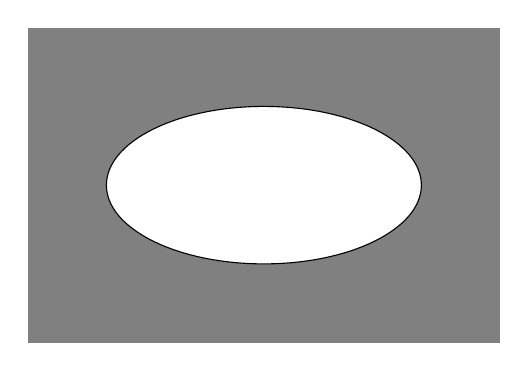
\begin{tikzpicture}[>=stealth, scale=1 ]
\fill [gray](-3,-2) rectangle(3,2);
\draw [fill=white] (0,0) ellipse [x radius=2, y radius=1];

\end{tikzpicture}
\caption{云母片上熔化了的石蜡成椭圆形}
\end{figure}

\begin{figure}[htp]\centering
	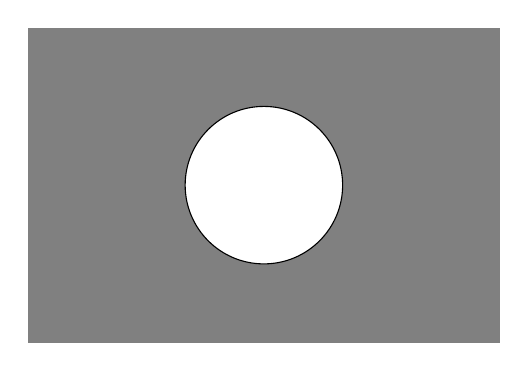
\begin{tikzpicture}[>=stealth, scale=1 ]
\fill [gray](-3,-2) rectangle(3,2);
\draw [fill=white] (0,0) circle [radius=1];

\end{tikzpicture}
\caption{玻璃板上熔化了的
石蜡成圆形}
\end{figure}

晶体可以分为单晶体和多晶体,如果整个物体就是一个晶体,这样的物体就叫做单晶体.上面说的晶体就是指单晶体.单晶体是科学技术上的重要原材料,制造各种晶体管就要用纯度很高的单晶硅或单晶锗.

如果整个物体是由许多杂乱无章地排列着的小晶体(晶粒)组成的,这样的物体就叫做\textbf{多晶体}.平常见到的各种金属材料就是多晶体.把纯铁做成的样品放在显微镜下观察,可以
看到它是由许许多多晶粒组成的.晶粒有大有小,最小的只有$10^{-5}$厘米那样大,最大的也超不过$10^{-3}$厘米.每个晶粒都是一个小单晶体,具有各向异性.由于晶粒在多晶体里杂乱无章地排列着,所以多晶体没有规则的几何形状,也不显示各向异性,它在不同方向上的物理性质是相同的,即各向同性.

\section{空间点阵}
十九世纪中叶,人们根据晶体外形的规则性和各向异性提出了一种假说,认为晶体内部的微粒是有规则排列着的,从1912年开始的应用X射线对晶体结构进行的研究,证实了这种假说的正确.现在,人们用电子显微镜对晶体内部结构进行直接观察和照相,进一步证实了这种假说的正确.

组成晶体的物质微粒(分子、原子或离子)依照一定的规律在空间中排成整齐的行列,构成所谓\textbf{空间点阵}.如果沿着这些物质微粒的行列画出直线来,可以得到若干组平行线,物质微粒就在这些组平行线的交点上.这些交点叫做空间点阵的
\textbf{结点}.

晶体中物质微粒的相互作用是很强的,微粒的热运动不足以克服它们的相互作用而远离,因而形成了空间点阵的结构.微粒的热运动主要表现为以结点为平衡位置不停地做微小的振动.
\begin{figure}[htp]\centering
	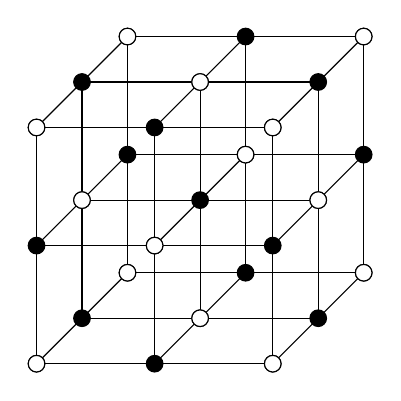
\begin{tikzpicture}[>=stealth, scale=1.5 ]
%\draw [->](0,0,0)--(0,0,10)node [right]{$z$};
%\draw [->](0,0,0)--(0,10,0)node [right]{$y$};
%\draw [->](0,0,0)--(10,0,0)node [right]{$x$};

%\draw (0,0,0) circle (2pt);
%\draw (0,0,2) circle (2pt);

\draw (0,0,0)--(0,0,2);
\draw (0,0,0)--(0,2,0);
\draw (0,0,0)--(2,0,0);
\draw (0,1,0)--(0,1,2);
\draw (0,1,0)--(2,1,0);
\draw (0,2,0)--(0,2,2);
\draw (0,2,0)--(2,2,0);
\draw (1,1,0)--(1,1,2);
\draw (1,2,0)--(1,2,2);
\draw (2,1,0)--(2,1,2);
\draw (2,2,0)--(2,2,2);
\draw (1,0,0)--(1,0,2);
\draw (1,0,0)--(1,2,0);
\draw (2,0,0)--(2,0,2);
\draw (2,0,0)--(2,2,0);
\draw(0,2,1)--(2,2,1);
\draw(0,2,2)--(2,2,2);
\draw(0,1,1)--(2,1,1);
\draw(0,1,2)--(2,1,2);
\draw (0,2,2)--(0,0,2);
\draw (2,0,2)--(0,0,2);
\draw (2,0,1)--(0,0,1);
\draw (2,0,2)--(2,2,2);
\draw (2,0,1)--(2,2,1);
\draw (1,0,1)--(1,2,1);
\draw (1,0,2)--(1,2,2);
\draw (0,0,1)--(0,2,1);


\foreach \x in {0,1,2}
\foreach \y in {0,1,2}
\foreach \z in {0,1,2}
{
\draw [fill=black](\x,\y,\z) circle (2pt);
}


\draw [fill=white] ( 0,0,0 )  circle (2pt);
\draw [fill=white] ( 0,0,2 )  circle (2pt);
\draw [fill=white] ( 0,1,1 )  circle (2pt);
\draw [fill=white] ( 1,0,1 )  circle (2pt);
\draw [fill=white] ( 2,0,0 )  circle (2pt);
\draw [fill=white] ( 2,0,2 )  circle (2pt);
\draw [fill=white] ( 2,1,1 )  circle (2pt);
\draw [fill=white] ( 1,2,1 )  circle (2pt);
\draw [fill=white] ( 0,2,0 )  circle (2pt);
\draw [fill=white] ( 0,2,2 )  circle (2pt);
\draw [fill=white] ( 1,1,0 )  circle (2pt);
\draw [fill=white] ( 1,1,2 )  circle (2pt);
\draw [fill=white] ( 2,2,0 )  circle (2pt);
\draw [fill=white] ( 2,2,2 )  circle (2pt);

\end{tikzpicture}
\caption{食盐晶体的空间点阵}
\end{figure}

图4.4是食盐的空间点阵示意图.食盐的晶体是由钠离子Na$^+$和氯离子Cl$^-$组成的,它们等距离地交错地排列在三
组相互垂直的平行线上,每个Na$^+$的周围有六个Cl$^-$,每个Cl$^-$的周围有六个Na$^+$.

晶体外形的规则性可以用物质微粒的规则排列来解释.
同样,晶体的各向异性也是由晶体的内部结构决定的.
\begin{figure}[htp]\centering
	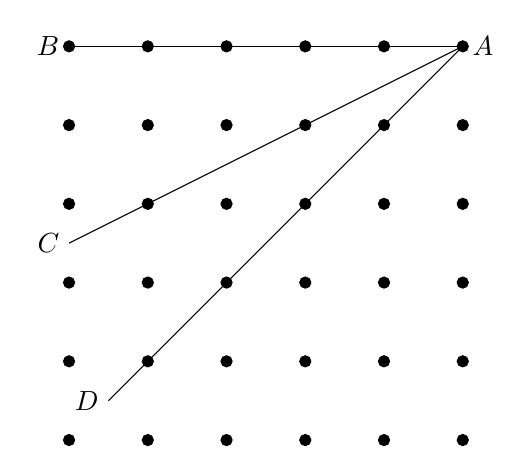
\begin{tikzpicture}[>=stealth, scale=1 ]

\foreach \x in {0,1,2,...,5}
\foreach \y in {0,1,2,...,5}
{
\draw [fill=black](\x,\y) circle (2pt);
}

\draw(0,5)node [left]{$B$}--(5,5)node [right]{$A$};
\draw (5,5)--(0,3-.5)node [left]{$C$};
\draw (5,5)--(.5,.5)node [left]{$D$};

\end{tikzpicture}
\caption{各向异性的微观解释}
\end{figure}

图4.5表示在一个平面上晶体物质微粒的排列情况.从图上可以看出,沿不同方向所画的等长直线$AB$、$AC$、$AD$上,物质微粒的数目不同.直线$AB$上物质微粒较多,直线$AD$上较少,直线$AC$上更少.正因为在不同方向上物质微粒的排列情况不同,才引起晶体在不同方向上物理性质的不同.

有的物质能够生成种类不同的几种晶体,是因为它们的物质微粒能够形成不同的空间点阵.例如,碳原子如果按图4.6那样排列就成为石墨,按图4.7那样排列就成为金刚石.石墨是层状结构,层与层之间距离较大,作用力较弱,沿着这个方向容易把石墨一层层地剥下.金刚石中碳原子间的作用力很强,所以金刚石有很大的硬度.
\begin{figure}[htp]\centering
	\begin{minipage}[t]{0.48\textwidth}
		\centering
\includegraphics[scale=1.3]{fig/4-6.pdf}
\caption{石墨的空间点阵}
	\end{minipage}
	\begin{minipage}[t]{0.48\textwidth}
		\centering
\includegraphics[scale=1.3]{fig/4-7.pdf}
\caption{金刚石的空间点阵}
	\end{minipage}
\end{figure}


\section{液体的微观结构}
液体的性质介于气体和固体之间.液体一方面象固体,具有一定的体积,不易压缩;另一方面又象气体,没有一定的形状,具有流动性.液体汽化时体积改变上千倍,凝固时体积改变不过百分之十.液体更接近于固体.

跟固体一样,液体中的分子也是密集在一起的,因而液体具有一定的体积,不易压缩.液体分子在很小的区域内作有规则的排列,这种区域是由分子暂时形成的,边界和大小随时改变,有时瓦解,有时又重新形成.液体由大量这种小区域构成,这种小区域杂乱无章地分布着,因而液体表现出各向同性.

液体分子间的距离小,相互作用力还很大,因此液体分子的热运动与固体类似,主要表现为在平衡位置附近做微小的振动,跟固体不同的是,液体分子没有长期固定的平衡位置,
在一个平衡位置附近振动一小段时间以后,又转到另一个平
衡位置附近去振动,即液体分子可以在液体中移动,这就是液体具有流动性的原因.

非晶体的微观结构跟液体非常类似,可以看作是粘滞性
极大的液体.所以严格说来只有晶体才能叫做真正的固体.

\section*{阅读材料:液晶}
某些有机化合物(现已发现有几千种)具有一种特殊的物质状态,叫做液晶.液晶一方面象液体,具有流动性;另一方面又象晶体,光学性质具有各向异性.液晶是介于液体和固体之间的过渡状态,微观结构也介于固液之间.

液晶是不稳定的,外界影响的微小变动都会引起液晶分子排列的变化,改变它的光学性质.有一种液晶,在外加电压的影响下,会由透明状态变成混浊状态,不再透明.去掉电压,又恢复透明,利用这一性质,可以制成显示元件.在两电极间将液晶涂成文字或数码,加上适当电压,透明的液晶变得混浊了,文字或数码就显示出来了.这种显示元件用于电子手表、电子计算器、微电脑以及其他仪器中.

还有一种液晶,具有灵敏的温度效应,温度改变时会改变颜色.只要温度升高1$^\circ$C,液晶就会按红、橙、黄、绿、蓝、靛、紫的顺序改变颜色;温度降低,又按相反顺序改变颜色.液晶的
这种性质,可以用来探测温度.例如在医学上可用来检查肿瘤.在皮肤表面涂上一层液晶,由于肿瘤部分的温度与周围正常组织的温度不一样,液晶会显示出不同的颜色,电路中的短路点温度高,用同样的办法可检查出短路点.

液晶早在十九世纪八十年代就被发现,直到电子技术和其他一些技术迅速发展起来以后,近十几年来,人们对液晶的研究才有了重要的进展,使它获得了广泛的应用.

\section{液体的表面现象}
荷叶上的小水滴、草叶上的露珠、玻璃板上的小水银滴都是近于球形的.大液滴呈扁平形状,是因为它本身的重量较大,它的形状受到重力的影响也比较大.如果设法消除重力的影响,大液滴也会呈球形.配制水和酒精的混合液,使它的密度跟橄榄油的密度相等.把橄榄油引入这种混合液里,可以看到橄榄油呈球形(图4.8).
\begin{figure}[htp]\centering
	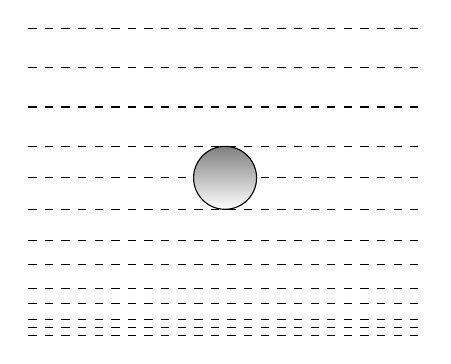
\begin{tikzpicture}[>=stealth, scale=1 ]

\foreach \x in {0,0.1,0.2,0.4,.6,.9,1.2,1.6,2,2.4,2.9,3.4,3.9}
{
  \draw [dashed](0,\x)--(5,\x);
}

\draw [shade] (2.5,2) circle (4mm);


\end{tikzpicture}
\caption{橄榄油在水和酒精的混合液里呈球形}
\end{figure}

我们知道,在体积相同的各种形状的物体中,球形物体的表面积最小,上述实验表明,液体表面有收缩到最小面积的趋势.

我们还可以用肥皂水做实验来证明液面具有收缩趋势.把一根棉线拴在铁丝环上(棉线不要张紧),把环在肥皂水里浸一下,使环上布满肥皂水的薄膜(图4.9甲).如果用热针刺破棉线左边的薄膜,棉线就被右边的薄膜拉成弧形(图4.9乙);如果刺破右边的薄膜,棉线就被左边的薄膜拉成弧形(图4.9丙).
\begin{figure}[htp]\centering
\includegraphics[scale=.45]{fig/4-9.png}
\caption{薄膜的收缩使棉线成弧形}
\end{figure}

\begin{figure}[htp]\centering
\includegraphics[scale=.45]{fig/4-10.png}
\caption{薄膜的收缩使棉线圈成圆形}
\end{figure}

把一个棉线圈拴在铁丝环上,使环上布满肥皂水的薄膜(图4.10甲).如果用热针刺破棉线圈里那部分薄膜,外边的薄膜就把棉线圈张紧成圆形(图4.10乙).

这些实验表明:液体的表面就好象张紧的橡皮膜一样,具有收缩的趋势.

为什么液体表面具有收缩的趋势呢?原来液体跟气体接触的表面形成一个薄层,叫做\textbf{表面层},表面层里的情况跟液体内部有所不同.研究表明,表面层里的分子要比液体内部稀疏些,也就是分子间的距离要比液体内部大些.在液体内部分子间既存在着引力,又存在着斥力.引力和斥力的数量级相同,在通常的条件下可以认为它们的大小是相等的.在表面层里分子间的距离大,引力和斥力都减小,但斥力减小得更快,所以分子间的相互作用表现为引力,如果在液面上划一条分界线$MN$(图4.11),把液面分为(1)和(2)两部分,那么,由于表面层中分子间的引力,液面(1)对液面(2)有引力$f_1$的作用,液面(2)对液面(1)
有引力$f_2$的作用,$f_1$和$f_2$大小相等
方向相反.象这种液面各部分间相互吸引的力,叫做\textbf{表面张力}.液体的表面张力使液面具有收缩的趋势.
\begin{figure}[htp]\centering
	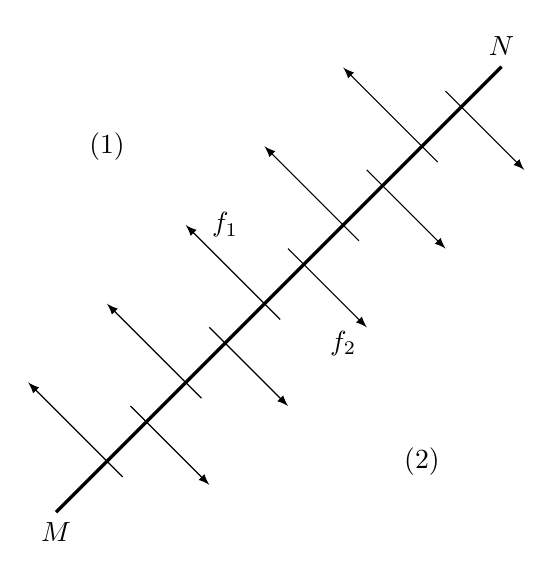
\begin{tikzpicture}[>=latex, scale=1 ]

\draw [very thick](45:.5)node[below]{$M$}--(45:8.5)node[above]{$N$};

\foreach \x in {1,2,...,5}
{ 
   \draw[->] (\x+.2,\x-.2)--(\x-1,\x+1);
   \draw[->] (\x+.5-.2,\x+.5+.2)--(\x+1.5-.2,\x-.5+.2);
}

\node at (1,5){(1)}; \node at (5,1){(2)};
\node at (4,2.5){$f_2$}; \node at (2.5,4){$f_1$};

\end{tikzpicture}
\caption{液体的表面张力}
\end{figure}

表面张力是跟液面相切的,如果液面是平面,表面张力
就在这个平面上;如果液面是曲面,表面张力就在这个曲面的切面上,作用在任何一部分液面上的表面张力,总是跟这部分液面的分界线垂直.

作用在液体表面单位长度分界线上的表面张力,叫做\textbf{表面张力系数}.不同液体的表面张力系数不同.分子间作用力大的液体,表面张力系数大,液态金属的表面张力系数很大,液态气体的很小.

\subsection*{练习一}
\begin{enumerate}
    \item 把玻璃管的裂断口放在火焰上烧熔,它的尖端就变圆.这是什么缘故?
\item 在处于失重状态的宇宙飞船中,一大滴水银会呈什么形状?
\item 把熔化的铅一滴一滴地滴入水中,凝固后可以得到
球形的小铅弹.为什么?
\end{enumerate}

\section{浸润和不浸润}
在洁净的玻璃板上放一滴水银,它能够在玻璃板上滚来滚去,而不附着在上面.把一块洁净的玻璃片浸入水银里再取出来,玻璃上也不附着水银,这种现象叫做\textbf{不浸润}.对玻璃来说,水银是不浸润液体.

在洁净的玻璃板上放一滴水,它要附着在玻璃板上形成薄层,把一块洁净的玻璃片浸入水里再取出来,玻璃片的表面是带有一层水的,这种现象叫做\textbf{浸润}.对玻璃来说,水是浸润液体.

同一种液体,对一些固体来说是浸润的,对另一些固体来说是不浸润的.水能浸润玻璃,但不能浸润石蜡,水银不能浸润玻璃,但能浸润锌.

把浸润液体装在容器里,例如把水装在玻璃容器里,由于水浸润玻璃,器壁附近的液面向上弯曲(图4.12),把不浸润液体装在容器里,例如把水银装在玻璃容器里,由于水银不浸润
玻璃,器壁附近的液面向下弯曲(图4.13),在内径较小的容器里,这种现象更显著,液面形成凹形或凸形的弯月面.

\begin{figure}[htp]\centering
	\begin{minipage}[t]{0.48\textwidth}
		\centering
	\begin{tikzpicture}[>=stealth, scale=.8]
\fill [pattern=north east lines](-.25,0) rectangle(0,5);
\fill [gray!20] (0,0) rectangle (3,3);
\fill [gray!20] (0,3)--(1,3)--(0,4);
\draw [fill=white, thick](0,4) arc(180:270:1);
\draw[thick](1,3)--(3,3);
\draw (0,0)--(0,5);
\fill [gray!20] (4, 0) rectangle (4.5, 5);
\draw [fill=white, rounded corners=0.2cm](4.5, 5)--(4.5, 4)--(4,4)--(4,5);
\draw (4, 0)--(4,5);
\draw (4.5, 0)--(4.5,5);
\end{tikzpicture}
\caption{液体浸润固体}
    \end{minipage}
\begin{minipage}[t]{0.48\textwidth}\centering
	\begin{tikzpicture}[>=stealth, scale=.8]

\fill [gray!50] (0,0) rectangle (3,2);
\fill [gray!50] (1,2) rectangle (3,3);
\fill [gray!50] (0,2)--(1,3)--(1,2);
\draw[ thick ](1,3)--(3,3);
\draw [fill=gray!50, thick ](1,3) arc(90:180:1);
\fill [white] (4, 0) rectangle (4.5, 5);
\draw [fill=gray!50, rounded corners=0.2cm](4.5, 0)--(4.5, 4)--(4,4)--(4,0);
\draw (4, 0)--(4,5);
\draw (4.5, 0)--(4.5,5);
\fill [pattern=north east lines](-.25,0) rectangle(0,5);
\draw (0,0)--(0,5);
\end{tikzpicture}
\caption{液体不浸润固体}
    \end{minipage}
\end{figure}

浸润和不浸润现象也是分子力作用的表现.当液体与固体接触时,在接触处形成一个液体薄层,叫做\textbf{附着层}.附着层里的分子既受到固体分子的吸引,又受到液体内部分子的吸引.如果受到的固体分子的吸引比较弱,附着层里的分子就比液体内部稀疏,在附着层就出现跟表面张力相似的收缩力,这时跟固体接触的液体表面有缩小的趋势,形成不浸润现象.相反,如果受到的固体分子的吸引相当强,附着层里的分子就比液体内部更密,在附着层里就出现液体相互推斥的力,这时跟固体接触的液体表面有扩展的趋势,形成浸润现象.

\subsection*{练习二}

\begin{enumerate}
   \item 把一根缝衣针小心地放在水面上,针可以把水面压弯而不沉没(试试看).解释这个现象.
   \item 布的雨伞虽然纱线间有可以看得出来的孔隙,却仍然不漏雨水.解释这个现象.
\end{enumerate}

\section{毛细现象}
把几根内径不同的细玻璃管插入水中,可以看到管里的水面比容器里的水面高.管的内径越小,管里的水面越高(图4.14).如果把这些细玻璃管插入水银中,发生的现象正好相
反,管里的水银面比容器里的水银面低.管的内径越小,管里
的水银面越低(图4.15).
\begin{figure}[htp]\centering
	\begin{minipage}[t]{0.48\textwidth}\centering
	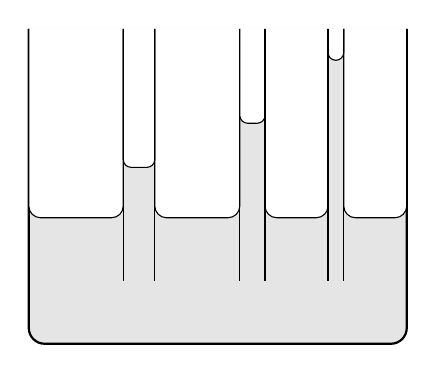
\begin{tikzpicture}[>=stealth, scale=.8 ]
\draw [fill=gray!20, rounded corners=0.2cm, thick](0,5)--(0, 0)--(6,0)--(6,5);
\draw [fill=white, rounded corners=0.15cm](0,5)--(0,2)--(1.5,2)--(1.5,5);
\draw [fill=white, rounded corners=0.15cm](2,5)--(2,2)--(3.35,2)--(3.35,5);
\draw [fill=white, rounded corners=0.15cm](3.75,5)--(3.75,2)--(4.75,2)--(4.75,5);
\draw [fill=white, rounded corners=0.15cm](5,5)--(5,2)--(6,2)--(6,5);


\draw [fill=white, rounded corners=0.1cm](1.5, 5)--(1.5,2.8)--(2, 2.8)--(2,5);
\draw [fill=white, rounded corners=0.1cm](3.35, 5)--(3.35,3.5)--(3.75, 3.5)-- (3.75, 5);
\draw [fill=white, rounded corners=0.1cm](4.75, 5)--(4.75, 4.5)--(5, 4.5)--(5, 5);

\foreach \x in {1.5,2,3.35,3.75,4.75,5}
{
  \draw (\x, 1)--(\x, 5);

}
\end{tikzpicture}
\caption{浸润液体在毛细管里上升
}
  \end{minipage}
\begin{minipage}[t]{0.48\textwidth}\centering
	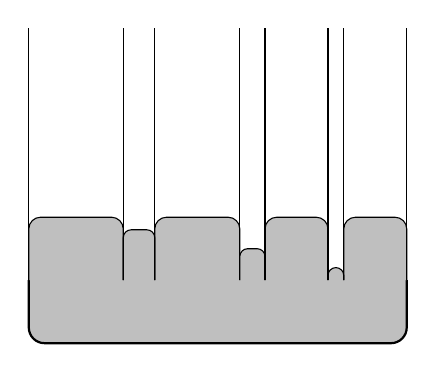
\begin{tikzpicture}[>=stealth, scale=.8 ]
\draw [fill=gray!50, rounded corners=0.2cm, thick](0,1)--(0, 0)--(6,0)--(6,1);

\draw [fill=gray!50, rounded corners=0.15cm](0,1)--(0,2)--(1.5,2)--(1.5,1);
\draw [fill=gray!50, rounded corners=0.15cm](2,1)--(2,2)--(3.35,2)--(3.35,1);
\draw [fill=gray!50, rounded corners=0.15cm](3.75,1)--(3.75,2)--(4.75,2)--(4.75,1);
\draw [fill=gray!50, rounded corners=0.15cm](5,1)--(5,2)--(6,2)--(6,1);


\draw [fill=gray!50, rounded corners=0.1cm](1.5, 1)--(1.5,1.8)--(2, 1.8)--(2,1);
\draw [fill=gray!50, rounded corners=0.1cm](3.35, 1)--(3.35,1.5)--(3.75, 1.5)-- (3.75, 1);
\draw [fill=gray!50, rounded corners=0.1cm](4.75, 1)--(4.75, 1.2)--(5, 1.2)--(5, 1);

\foreach \x in {0,1.5,2,3.35,3.75,4.75,5,6}
{
  \draw (\x, 1)--(\x, 5);

}



\end{tikzpicture}
\caption{不浸润液体在毛细管里下降
}
    \end{minipage}
\end{figure}

象这样浸润液体在细管里上升的现象和不浸润液体在细管里下降的现象,叫做\textbf{毛细现象}.发生毛细现象的管叫做毛细管.

浸润液体为什么能在毛细管里上升呢?原来,浸润液体跟毛细管内壁接触时,引起液面的弯曲,使液面变大.而表面张力的收缩作用使液面减小,于是管内液体随着上升,以减小液面.直到表面张力向上的拉引作用和管内升高的液柱的重量达到平衡时,管内液体停止上升,稳定在一定的高度.利用类似的分析,也可以解释不浸润液体在毛细管里下降的现象.

纸张、棉花、毛巾、粉笔、木材、土壤、砖块等物体,内部有
许多细小的孔道,起着毛细管作用,所以它们能够吸水,这就是用毛巾擦汗、灯芯吸油、粉笔吸墨水的道理.

毛细现象在农业生产上有非常重要的意义,土壤里有很多毛细管,地下的水分可以沿着它们上升到地面.如果要保存地下的水分来供植物的根吸收,就要把地面的土壤锄松,破
坏这些土壤里的毛细管.相反,如果想把地下的水分引上来,就不仅要保持土壤里的毛细管,而且还要使它们变得更细,这时就要用滚子压紧土壤.

\subsection*{练习三}
\begin{enumerate}
   \item 要想把凝在衣料上面的蜡或油脂去掉,只要把两层吸墨纸分别放在这部分衣料的上面和下面,然后用熨斗来熨就可以了,为什么这样做可以去掉衣料上的蜡或油脂?
\item 建筑楼房的时候,在砌砖的地基上铺一层油毡防潮层.如果不铺这层油毡,楼房就容易受潮,为什么?
\end{enumerate}

\section*{复习题}

\begin{enumerate}
\item 晶体和非晶体在外形和物理性质上有什么区别?
\item 什么叫空间点阵?怎样从微观上解释晶体具有规则的外形和各向异性?
\item 液体的微观结构是怎样的?
\item 什么叫表面张力?为什么液体表面具有收缩趋势?
\item 什么叫浸润,什么叫不浸润?怎样解释浸润現象和不浸润现象?
\item 什么叫毛细现象?为什么会发生毛细现象?
\end{enumerate}



 %固体和液体的性质
	%\chapter{物态变化}\label{chapter-change-of-state-of-matter}

固体、液体和气体是通常存在的三种物质状态.在一定条件下,这三种物质状态可以相互转化,即发生物态变化,水结成冰或变成水蒸气就是常见的物态变化的例子.物态变化跟日常生活和工农业生产有密切关系,有许多实际应用.
在初中我们学过一些物态变化的知识,这一章进一步扩大和加深这方面的知识,同时学习一些新知识.

\section{熔解和凝固}
物质从固态变成液态叫做\textbf{熔解},从液态变成固态叫做\textbf{凝固}.

我们知道,固体分晶体和非晶体.晶体物质和非晶体物质在熔解和凝固时情况是不同的.晶体有一定的熔解温度——\textbf{熔点}.给晶体加热,当温度升高到熔点时,晶体开始熔解,在熔解过程中温度保持不变,到全部熔解后,温度才继续上升.它们的液体冷却时,温度降低到熔点时开始凝固,在凝固过程中温度也保持不变,到全部凝固后,温度才继续下降.

非晶体没有一定的熔点.
温度升高时,非晶体先是由硬变软,再逐渐变成粘稠状液体,最后逐渐变成液体.在整个过程中,温度不停地上升,没有一定的熔解温度.
冷却时,随着温度
的下降,液体由稀变稠,由软变硬,最后成为固体.
在整个过程中,温度不停地下降,没有一定的凝固温度.

晶体物质熔解和凝固时的特点,可用晶体的微观结构来解释.在晶体中,微粒排列成有规则的空间点阵,维持这种规则排列的是微粒之间的相互作用;微粒的热运动不足以克服这种相互作用,微粒一般只能在平衡位置附近做无规则的振动.给晶体加热时,晶体从外界得到能量,微粒的热运动加剧.达到一定的温度时,一部分微粒具有了足够的动能,能够克服微粒间的作用力,离开平衡位置.这时晶体的点阵结构被破坏,晶体开始熔解.
在熔解过程中,外界供给晶体的能量,全部用来破坏晶体的点阵结构,增加分子间的势能,所以温度不发生变化.凝固时,情况正好相反.微粒排列成点阵结构时,微粒间的势能减小,因此虽然放出能量,温度却保持不变,直到全部凝固成晶体.

非晶体的微观结构本来就跟液体类似,非晶体在熔解过
程中不必为破坏点阵结构而消耗能量,所以温度不停地上升.

实验表明,大多数物质熔解时体积膨胀,凝固时体积缩小.然而也有少数物质跟上述情况相反,例如水、灰铸铁、锑、铋等,它们在熔解时体积缩小,凝固时体积膨胀.用铸铁浇铸成的工件,形状跟铸模完全相似,正是利用了铸铁凝固时体积膨胀的特点.水结冰时体积膨胀,所以在冬季水管和盛水的容器常会冻裂,需要加以防止.

物质的熔点跟压强有关系.
熔解时体积膨胀的物质,如果所受的压强增大,熔解将受到阻碍,只有在更高的温度下才能熔解,所以熔点升高.
熔解时体积缩小的物质,如果所受的压强增大,会促进熔解的进行,所以熔点降低.冰在熔解时体积缩小,因而冰在受到巨大的压强时,在0$\Ucede$以下也能熔解.不过压强对熔点的影响并不显著,例如,每增加1标准大气压,冰的熔点才降低0.0075$\Ucede$.

表~\ref{tab_B_5-1} 列出了几种物质在1标准大气压下的熔点.

\begin{table}[htbp]
	\centering
	\caption{}\label{tab_B_5-1}
	\begin{tblr}{cc|cc}
	\toprule
	物质 & 熔点($\UcedeA$) & 物质 & 熔点($\UcedeA$) \\
	\midrule
	氦 & $-$272 & 铅 & 327\\
	氢& $-$259 & 铝 & 660\\
	酒精& $-$117 & 银 & 962\\
	氨& $-$77.7 & 金 & 1064\\
	水银& $-$39 & 铜 & 1083\\
	冰& 0 & 铁 & 1535\\
	萘&80 & 钨 & 3410\\
	锡&232   & 碳 & 3550\\
	\bottomrule
	\end{tblr}
\end{table}

一般说来,纯物质中掺进另一种物质,熔点要降低.例如
海水比淡水的熔点低.冰和食盐的混合物,熔点可以降低到零下二十多摄氏度.
冰和氯化钙的混合物,熔点可以降低到零下五十多摄氏度.

某些合金的熔点较低.
例如铅锑合金的熔点为246$\Ucede$,锡铅合金的熔点为170$\Ucede$,由铋、镉、锡、铅组成的伍德合金,其熔点仅 70$\Ucede$.
这些低熔点合金在生产技术中具有广泛的应用.

熔点是物质的重要性质之一,在实际中常常要根据需要选用不同熔点的物质.
例如,制做白炽灯丝要用熔点高的钨,
而焊接电路则用熔点较低的铅锡合金.

\section{熔解热}
晶体在熔解过程中不断从外界吸收热量,但温度却保持不变.吸收的热量绝大部分用于破坏晶体的点阵结构,增加分子势能.
对大多数熔解时体积增大的物质来说,还有一部分热量用来克服外界压强做功.不过体积变化不大,这个功很小.

质量相等的不同晶体溶解时吸收的热量是不同的.\textit{单位质量的某种物质熔解成同温度的液体时吸收的热量,叫做这种物质的\textbf{熔解热}}.在国际单位制中,熔解热的单位是焦/千克($\UJkgA$).

液体凝固时要放出热量.单位质量的某种物质凝固时放出的热量等于它的熔解热.显然这是符合能量守恒定律的.

物质的熔点跟压强有关系,在不同的熔解温度下,物质的熔解热也略有不同.表~\ref{tab_B_5-2} 列出了几种物质在1标准大气压下的熔解热.

\begin{table}[htbp]
	\centering
	\caption{}\label{tab_B_5-2}
    \begin{tblr}{cc|cc}
  \toprule
 物质 & 熔解热($\UJkgA$) & 物质 & 熔解热($\UJkgA$) \\
  \midrule
  铝 & $3.96\times 10^5$ & 萘 & $1.51\times 10^5$\\
  冰& $3.35\times 10^5$ & 锡 & $0.6\times 10^5$\\
  镍& $2.99\times 10^5$ & 铅 & $0.25\times 10^5$\\
   铁& $2.67\times 10^5$ & 水银 & $0.11\times 10^5$\\
  铜& $2.05\times 10^5$ & 二氧化碳 & $1.81\times 10^5$\\
   钨& $1.92\times 10^5$ & 金 & $0.64\times 10^5$\\
    \bottomrule
   \end{tblr}
\end{table}

熔解热常用字母$\lambda$表示.知道了熔解热,就可以算出质量为$m$的物质熔解时吸收的热量$Q$:
\[Q=\lambda m \]

熔解热可以用量热器测定.现在以冰为例来说明.在量热器中装入已知质量的水,测出水的温度,然后把正在熔解的冰块(温度为0$\Ucede$)放入量热器的水中,冰将继续熔解,水的温度下降.测出冰块全部熔解后水的末温度和水的质量.根据前后两次测得的水的质量,可以求出冰块的质量.
冰块熔解成水并从0$\Ucede$升高到末温度吸收的总热量,等于量热器中原来的水和小筒从初温度下降到末温度放出的热量.
从这个关系就可以求出冰的熔解热.

例如,如果已知铜制量热器小筒的质量是150克,里面装着100克16$\Ucede$的水.放入9克0$\Ucede$的冰,冰完全熔解后水的温度是9$\Ucede$.利用这些数据就可以求出冰的熔解热.

9克0$\Ucede$的冰熔解为0$\Ucede$的水,再升高到9$\Ucede$,总共吸收
的热量
\[Q_{\text{吸}}=m_{\text{冰}}\lambda +m_{\text{冰}}c_{\text{水}} (9\Ucede-0\Ucede) \]
量热器中的水和量热器小筒从16$\Ucede$降到9$\Ucede$放出的热量
\[Q_{\text{放}}=m_{\text{水}}c_{\text{水}} (16\Ucede-9\Ucede) +m_{\text{筒}}c_{\text{铜}} (16\Ucede-9\Ucede) \]
因为$Q_{\text{吸}}=Q_{\text{放}}$,所以
\[m_{\text{冰}}\lambda +m_{\text{冰}}c_{\text{水}} (9\Ucede-0\Ucede)=\left(m_{\text{水}}c_{\text{水}}  +m_{\text{筒}}c_{\text{铜}}\right) (16\Ucede-9\Ucede) \]

统一单位后,把数值代入上式[铜的比热$c_{\text{铜}}=3.9\times 10^2  \UJkgcede $],可得
\[\lambda=3.3\times 10^5 \UJkg   \]

冰的熔解热很大,1千克0$\Ucede$的冰熔解成0$\Ucede$的水吸收的热量,相当于把1千克0$\Ucede$的水升高到80$\Ucede$需要的热量.冰的这一特点对自然界有重要的意义,它使得初冬时,一个寒冷的夜晚不会把江河湖全部封冻起来,气温也不会骤然下降;初春时,一个阳光灿烂的晴天不会使冰雪全部熔解,造成江河泛滥,气温也不会骤然升高.在日常生活中,人们利用冰熔解热大的特点来冷藏食品、冰镇饮料等.

\subsection*{练习一}

\begin{enumerate}
    \item 把玻璃放在火上加热,观察它的熔解情况,看看玻璃是不是先变软,再流动.玻璃是不是晶体?
    \item 解释下面的现象:把一块冰放在支承物上(图~\ref{fig_B_5-1}),
    将两端各挂一个重物的铁丝搭在冰块上.过一段时间后可以看到,铁丝切进冰块,但是铁丝穿过冰块的地方并没有留下切口,冰仍然是完整的一块.
    铁丝为什么能切进冰块?铁丝穿过后上面的冰为什么又成了完整的一块?如果有条件,自己做一做这个实验.
    \begin{figure}[htbp]
      \centering
      \includegraphics{fig/B/5-1.pdf}
      \caption{细铁丝穿过冰块而不留下切口}\label{fig_B_5-1}
    \end{figure}
    \item   冬季在菜窖里放上几桶水,可以使窖内的温度不致降低得很多,防止把菜冻坏.这是什么道理?如果在窖内放入200千克10$\Ucede$的水,试计算这些水结成0$\Ucede$的冰时放出的热量.这相当于燃烧多少千克干木柴所放出的热量?干木柴的
    燃烧值约为$1.26\times 10^4 \UkJkg$.
\item  铜制量热器小简的质量是160克,装入200克20$\Ucede$的水.向水里放进30克0$\Ucede$的冰,冰完全熔解后水的温度是多少摄氏度?
\item  量热器的铜制小筒里盛有200克15$\Ucede$的水,小筒的质量为160克.
向水里放入50克0$\Ucede$的冰,求量热器里的末温度是多少摄氏度?
\end{enumerate}


\section{蒸发}
物质从液态变成气态,叫做汽化.汽化有两种方式:蒸发和沸腾.蒸发是在液体表面进行的汽化现象.这一节我们先来研究蒸发.

我们知道,液体中的分子都在不停地运动着,它们的平均动能跟温度有关系.但在任何温度下,总有一部分分子的动能比平均动能大.那些处在液体表面层附近的动能足够大的分子,能够挣脱周围分子的引力,飞出液面,形成蒸气,这就是\textbf{蒸发}.
蒸气也常叫做汽.

液体温度越高,分子的平均动能就越大,具有足够大的动能因而能够飞出液面的分子也就越多.所以,温度越高,蒸发得越快.泼在地上的水夏天干得快,冬天干得慢,就是这个原因.

液体的表面积越大,处在表面层中的分子就越多,能够从液面飞出的分子也就越多.所以,表面积越大,蒸发得越快.洗过的衣服抻开晾晒比团在一起干得快,原因就在这里.

飞出液面的分子如果停留在液面附近,由于分子的热
运动,有的分子会撞到液面,被液体分子重新拉回到液体中去,这样蒸发就变慢了.如果设法把液面上形成的蒸气吹散,使汽分子不能回到液体中去,蒸发就可以加快.所以,蒸发的快慢还跟液面上气体流动的快慢有关系.气体流动得越快,蒸发得也越快.
这就是吹风能够使湿东西干得快的原因.

在同样的条件下,不同液体蒸发得快慢不同.水比食油容易蒸发,汽油比水容易蒸发.容易蒸发的液体,我们常说它的挥发性大.液体的这种差别,跟它们分子间的作用力有关系.分子间作用力大的液体不容易蒸发.

在蒸发过程中,从液体中飞出的是动能较大的分子,这些分子飞出后,留在液体中的分子的平均动能必然减小,所以蒸发时液体的温度降低.
这时它就要从周围的物体吸收热量,因而液体蒸发有致冷作用.穿湿衣服比穿干衣服感到冷,夏天搧扇子感到凉快,出汗后站在通风处容易着凉,都是由于蒸发致冷的缘故.蒸发致冷作用在实际中有许多应用.用火车运送容易腐烂变质的食品时,常用液态氨或液态二氧化碳的蒸发来降低车厢内的温度.在医疗中,可用液态氮迅速蒸发时的冷却作用使病灶处的细胞冷冻坏死.导弹在大气中高速飞行时,由于跟空气摩擦,会达到极高的温度.为了保护弹壳,常在弹壳表面涂上防护层,防护层的物质受热熔解和蒸发时,要
吸收大量的热量,从而降低了导弹表面的温度.

\section{饱和汽与饱和汽压}
\subsection{饱和汽} 
装在敞口容器里的液体,由于蒸发出来的汽分子能够分散到周围空间里去,所以过一段时间后液体会全部蒸发完.
盛在密闭容器里的液体,即使过很长时间,也不会蒸发完,这是什么原因呢?原来在容器中的液面上同时进行着两种相反的过程:一方面分子从液面飞出来;另一方面由于液面上的汽分子不停地做无规则的热运动,有的汽分子撞到液面上又会回到液体中去(图~\ref{fig_B_5-2}).在密闭的容器中,随着液体的
不断蒸发,液面上汽的密度不断增大,回到液体中的分子数也逐渐增多.
最后,当汽的密度增大到一定程度时,就会达到这样的状态:在单位时间内回到液体中的分子数等于从液面飞出去的分子数.这时汽的密度不再增大,液体也不再减少,
液体和汽之间达到了平衡状态,这种平衡叫做\textbf{动态平衡}.我们把跟液体处于动态平衡的汽叫做\textbf{饱和汽}.把没有达到饱和状态的汽叫做\textbf{未饱和汽}.在一定温度下,饱和汽的密度是一定的,未饱和汽的密度小于饱和汽的密度.

\begin{figure}[htbp]
  \centering
  \includegraphics{fig/B/5-2.pdf}
  \caption{}\label{fig_B_5-2}
\end{figure}

饱和汽的密度随着温度而改变.温度升高时,液体分于的平均动能增大,单位时间里从液面飞出的分子数增多,原来的动态平衡被破坏,液体就继续蒸发,汽的密度继续增大,直
到达到新的动态平衡为止.所以饱和汽的密度随着温度的升高而增大.温度降低时,饱和汽的密度减小.其原因请同学们自己来解释.

\subsection{饱和汽压} 

某种液体的饱和汽所具有的压强,叫做这种液体的饱和汽压.用下面的实验可以测量饱和汽压.把两根装满水银的细长玻璃管倒立在水银槽中(图~\ref{fig_B_5-3}).$a$管用作气压计.用弯曲玻璃管向$b$管中注入一些乙醚.乙醚的密度比水银小,便浮到水银面上,并在水银面上方的真空中蒸发,
同时$b$管中的水银面开始下降.
当乙醚汽的密度达到饱和时,水银面上还剩有一点乙醚,$b$管中的水银面就稳定在一定的高度不再下降.$a$、$b$两管中水银面的高度差$h$就表示乙醚饱和汽压的大小.如果不用乙醚,而是向$b$管中注入水或酒精,就可以测出水或酒精的饱和汽压.
\begin{figure}[htbp]
  \centering
  \includegraphics{fig/B/5-3.pdf}
  \caption{测量饱和汽的压强}\label{fig_B_5-3}
\end{figure}

实验表明,在相同的温度下,不同液体的饱和汽压一般是不同的.挥发性大的液体,饱和汽压大.例如,20$\Ucede$时,乙醚的饱和汽压为440毫米汞柱,水为18毫米汞柱,水银的饱和汽压很小,20$\Ucede$时仅为0.0012毫米汞柱.所以水银气压计水银柱上方的空间可以认为是真空.

\subsection{饱和汽压跟温度的关系} 

用热毛巾把图~\ref{fig_B_5-3} 中的$b$管包住,使管内的温度升高,可以看到管中的水银面下降.这表示温度升高时饱和汽压增大.如果使管内的温度降低,管中的水银面就上升,表示温度降低时饱和汽压减小.可见,\textit{饱和汽压随温度的升高而增大,随温度的降低而减小.}

饱和汽压随温度的升高而增大,这是由两方面的原因引起的.
一个原因是温度升高时,饱和汽的密度增大,因此压强增大.
另一个原因是温度升高时,汽分子热运动的平均速率增大,这也使得压强增大.图~\ref{fig_B_5-4} 是水的饱和汽压与温度的关系图线.从图线可以看出,温度升高时,饱和汽压增大,但是饱和汽压与温度的关系不是线性的,饱和汽压随温度的升高增大得很快.
\begin{figure}[htbp]
  \centering
  \includegraphics{fig/B/5-4.pdf}
  \caption{水的饱和汽压与温度的关系图线}\label{fig_B_5-4}
\end{figure}

饱和汽压随温度的降低而减小,其原因同学们可以自己分析一下.

\subsection{饱和汽压跟体积的关系} 

现在我们用实验来研究饱和汽
压跟体积的关系.像图~\ref{fig_B_5-5} 那样,把水银倒在一个深的容器里,再把装满水银的玻璃管倒立在这个容器中.向玻璃管里移入一些乙醚,使乙醚蒸发后水银面上还留有少量液态乙醚.这时管内乙醚的饱和汽压等于$p_0-p_h$(图~\ref{fig_B_5-5a}),其中$p_0$是大气压强.
\begin{figure}[htbp]
    \centering
    \begin{subfigure}{0.3\linewidth}
        \centering
        \includegraphics{fig/B/5-5a.pdf}
        \caption{}\label{fig_B_5-5a}
    \end{subfigure}
    \hfil
    \begin{subfigure}{0.3\linewidth}
        \centering
        \includegraphics{fig/B/5-5b.pdf}
        \caption{}\label{fig_B_5-5b}
    \end{subfigure}
    \hfil
    \begin{subfigure}{0.3\linewidth}
        \centering
        \includegraphics{fig/B/5-5c.pdf}
        \caption{}\label{fig_B_5-5c}
    \end{subfigure}
    \caption{饱和汽压跟体积无关}\label{fig_B_5-5}
\end{figure}

现在把管子往上提高一些,使水银面上乙醚汽的体积增大(图~\ref{fig_B_5-5b}),可以看到,水银面上的液态乙醚减少了,
但是管里水银柱的高度还跟原来一样.这表明,在温度不变的情况下,体积增大时饱和汽压不改变.

把提高的管子放下一些,使乙醚汽的体积减小(图~\ref{fig_B_5-5c}). 这时水银面上的液态乙醚增多,但是管中水银柱的高度仍保持不变.这表明,在温度不变的情况下,体积减小时饱和汽压也不改变.

在温度不变的情况下,饱和汽的压强不随体积而变化,可作如下的解释:当体积增大时,容器中汽的密度减小,原来的饱和汽变成了未饱和汽,于是液体继续蒸发,直到未饱和汽成为饱和汽为止;由于温度没有改变,新的饱和汽的密度跟原来的一样,汽分子热运动的平均速率也跟原来一样,所以压强不
改变.体积减小时,容器中汽的密度增大,回到液体中的分子数多于从液面飞出的分子数,于是一部分汽变成液体,直到汽的密度减小到等于该温度下饱和汽的密度为止;由于温度跟原来相同,饱和汽的密度不变,汽分子热运动的平均速率也跟原来相同,所以压强也不改变.

从上面讲的可以看出,饱和汽的压强跟体积没有关系,饱和汽的压强与温度的关系不是线性的,这些都跟理想气体的情况不同.因此,第\ref{chapter-properties-of-gases}章所讲的理想气体定律对饱和汽是不适用的.


\subsection*{练习二}

\begin{enumerate}
\item 举出几个蒸发致冷的例子来.
\item 液面上的汽达到饱和时,还有没有液体分子从液面飞出?为什么这时从宏观上看来液体不再蒸发?
\item 饱和汽的密度怎样随温度而变化?饱和汽的压强怎祥随温度而变化?为什么这样变化?
\item 在温度不变的情况下,增大液面上饱和汽的体积时,下面的说法哪些是正确的:
\begin{enumerate}
    \item 饱和汽的质量不变,饱和汽的密度减小;
    \item 饱和汽的密度不变,饱和汽的压强也不变;
    \item 饱和汽的密度不变,饱和汽的压强增大;
    \item 饱和汽的质量增大,饱和汽的压强也增大;
    \item 饱和汽的质量增大,饱和汽的压强不变.
\end{enumerate}

\item 解释下面的现象:密闭容器中装有少量液态乙醚,当容器的温度升高时,液态乙醚逐渐减少;容器升高到一定温度
时,液态乙醚消失;容器冷却时,容器中又出现液态乙醚.
\end{enumerate}

\section{沸腾}
给液体加热,当液体升高到一定温度时,液体内部涌现出大量的气泡,升到液面破裂开,放出汽.这时整个液体发生剧烈的汽化,这种现象叫做\textbf{沸腾}.

现在我们来研究一下水的沸腾过程.
给盛水的烧杯加热,原来吸附在杯底和杯壁上的空气以及溶解在水里的空气就分离出来,形成一些小气泡.由于周围的水向气泡里蒸发,所以气泡里包含的是饱和水汽和空气.杯底受热温度升高时,气泡膨胀,当体积胀大到一定程度时,气泡就脱离杯底浮起.在达到沸腾温度以前,气泡在上升过程中体积是逐渐缩小的(图~\ref{fig_B_5-6a}).
这些小气泡升到液面破裂时,放出的主要是空气.
\begin{figure}[htbp]
    \centering
    \begin{subfigure}{0.4\linewidth}
        \centering
        \includegraphics{fig/B/5-6a.pdf}
        \caption{}\label{fig_B_5-6a}
    \end{subfigure}
    \hfil
    \begin{subfigure}{0.4\linewidth}
        \centering
        \includegraphics{fig/B/5-6b.pdf}
        \caption{}\label{fig_B_5-6b}
    \end{subfigure}
    \caption{}\label{fig_B_5-6}
\end{figure}

当杯内水的温度都升高到某一温度,气泡内的饱和汽压等于外界压强时,气泡在上升过程中体积就不再缩小.并且
由于在上升过程中周围的水还在不断向泡内蒸发,所以体积还会继续增大,直到升到液面破裂开(图~\ref{fig_B_5-6b}).这时从气泡里放出的主要是水蒸气.
这时水就沸腾了.沸腾时,在液体表面和液体内部同时发生汽化,这是沸腾和蒸发的主要区别.

从上面水的沸腾过程可以看出,\textit{液体只有在它的饱和汽压等于外界压强时才能沸腾.}在外界压强是1标准大气压的情况下,水在100$\Ucede$沸腾,就是因为100$\Ucede$时水的饱和汽压为760毫米汞柱,等于外界的大气压强.

液体沸腾时的温度叫做\textbf{沸点}.外部压强改变时,液体的沸点也改变.在外部压强增大时,液体需要升到较高的温度时饱和汽压才能等于外部压强,所以沸点升高.在外部压强
减小时,液体在较低的温度下饱和汽压就能等于外部压强,所以沸点降低.上述结论可以用实验来证明.把一杯温度低于100$\Ucede$的热水放在抽气机的玻璃罩里,抽出罩里的空气,当罩里空气的压强降低到一定程度时,热水就沸腾起来(图~\ref{fig_B_5-7}).
\begin{figure}[htbp]
  \centering
  \includegraphics{fig/B/5-7.pdf}
  \caption{压强减小时水的沸点降低}\label{fig_B_5-7}
\end{figure}

离海平面越高,大气压强越小,所以高山上水的沸点较低.珠穆朗玛峰顶的气压大约只有1/3标准大气压,在那里水烧到约72$\Ucede$就沸腾了.
在海拔高的山上,由于沸点低,用
普通锅煮不熟饭,需要用高压锅.高压锅内的水蒸气不容易泄出来,锅内的压强可以达到2标准大气压,锅内水的沸点接近120$\Ucede$,所以用高压锅煮饭热得快.工业上用的蒸汽锅炉也是利用增大压强来提高沸点,获得高温高压蒸汽的.如果锅炉中压强接近大气压强的10倍,水的沸点就可提高到180$\Ucede$左右.

在相同的压强下,各种物质的沸点不同.例如,在1标准大气压下,乙醚的沸点为35$\Ucede$,酒精的沸点为78$\Ucede$.利用物质的这一性质,可以对液体混合物进行分馏:给液体混合物加热,其中沸点较低的成份先蒸发出来,沸点较高的成份后蒸发出来.汽油、煤油、柴油就是在炼油厂中对石油进行分馏而得到的.

\section{汽化热}
水沸腾后,虽然继续给它加热,但是水的温度并不上升,只是有更多的水变成了水蒸气.可见,水在沸腾过程中要吸收热量.液体变为蒸气时,体积膨胀,分子间的距离增大.沸腾过程中吸收的热量,一部分用来克服分子间的引力做功增大分子势能,另一部分用于体积膨胀时克服外界压强做功.

\textit{单位质量的某种液体,变为同温度的气体时吸收的热量,叫做这种液体的\textbf{汽化热}.}

汽化热常用字母$L$表示.在国际单位制中,汽化热的单位是焦/千克($\UJkgA$).

不同物质的汽化热不同.表~\ref{tab_B_5-3} 列出了一些物质在1标准
大气压下沸点时的汽化热.

\begin{table}[htbp]
	\centering
	\caption{}\label{tab_B_5-3}
	\begin{tblr}{ccc|ccc}
	\toprule
	物质  & 沸点&汽化热&  物质  & 沸点 &汽化热\\
	&($\UcedeA$)&($\UJkgA$)&& ($\UcedeA$)&($\UJkgA$)\\
	\midrule
	液态氦 &$-269$& $2.50\times 10^4$ &乙醚 &35& $3.52\times 10^5$\\
	液态氢&$-253$& $4.53\times 10^5$ &酒精&78& $8.55\times 10^5$\\
	液态氧&$-183$& $2.14\times 10^5$ &水&100& $2.26\times 10^6$\\
	液态二氧化碳&$-78.5$& $2.30\times 10^5$ &水银&357& $2.89\times 10^5$\\
	液态氨&$-33$& $1.37\times 10^6$ &液态铁&2750& $6.30\times 10^6$\\
	\bottomrule
	\end{tblr}
\end{table}

汽凝结为液体时要放出热量.实验表明,单位质量的汽凝结为液体时放出的热量,
等于在同一温度下液体变为相同温度的汽时的汽化热.

知道了物质的汽化热$L$,就能计算出质量为$m$的液体变为同温度的汽时吸收的
热量或质量为$m$的汽变为同温度的液体时放出的热量:
\[Q=Lm\]

在不同温度下,同一物质的汽化热不同.温度升高时,物质的汽化热变小,
这是因为温度升高时液体分子间的距离增大,液体变为汽时克服分子间的引力需
要做的功减小.

表~\ref{tab_B_5-4} 是水在不同温度下的汽化热.

\begin{table}[htbp]
	\centering
	\caption{}\label{tab_B_5-4}
	\begin{tblr}{cc|cc}
	\toprule
	温度($\UcedeA$)&汽化热($\UJkgA$)
	&温度($\UcedeA$)&汽化热($\UJkgA$)\\
	\midrule
	0& $2.50\times 10^6$ & 200 & $1.96\times 10^6$ \\
	50& $2.38\times 10^6$ & 300 & $1.38\times 10^6$ \\
	100& $2.26\times 10^6$ & 370 & $4.14\times 10^5$ \\
	\bottomrule
	\end{tblr}
\end{table}



水的汽化热可以用图~\ref{fig_B_5-8} 所示的实验装置来测定.用酒
精灯把烧瓶A里的水加热至沸腾.从烧瓶A里出来的蒸汽,经过试管$B$
进入装着水的量热器小筒$C$中.蒸汽经过试管$B$后,其中所含的小水滴留下来,
使得进入量热器的蒸汽中不含有水滴.蒸汽在小筒$C$中凝结时放出热量,
使小筒里的水和小筒本身的温度升高.
到水温升高到相当的度数时,停止通入蒸汽.
小筒$C$的质量$m$以及其中水的质量$m_1$和温度$t_1$已在通入蒸汽前测出.
停止通入蒸汽后,再测出水的末温度$t_2$和质量$m_2$,$m_2-m_1$就是通入水中的蒸汽的质量.
水和小筒从温度$t_1$升高到$t_2$吸收的热量等于100$\Ucede$的蒸汽变为$t_2$的水放出的热量,
利用这个关系就可以求出水在100$\Ucede$时的汽化热.

\begin{figure}[htbp]
	\centering
	\includegraphics{fig/B/5-8.pdf}
	\caption{测定水的汽化热}\label{fig_B_5-8}
\end{figure}


\subsection*{练习三}
\begin{enumerate}
\item 在1标准大气压下,乙醚的沸点是35$\Ucede$.这个温度时乙醚的饱和汽压是多大?
\item 锡的熔点是232$\Ucede$,但是用锡焊的水壶盛着水放在1000$\Ucede$以上的火上烧,锡并不熔解.为什么?
\item 在蒸汽暖室装置的散热器里,每小时有20千克100$\Ucede$的水蒸气液化成水,
并且水的温度降低到80$\Ucede$.求散热器每小时供给房间的热量.
\item 某人在做测定水的汽化热实验时,得到的数据如下:
钢制量热器小筒的质量为200克,通入水蒸气前筒内水的质量为350克,温度为14$\Ucede$;
通入100$\Ucede$的水蒸气后水的温度为36$\Ucede$,水的质量为364克.
他测得的水的汽化热是多少?
\item 容器里装有0$\Ucede$的冰和水各500克,向里面通入100$\Ucede$的水蒸气后,
容器里的水升高到了30$\Ucede$.假设容器吸收的热量很少,可以忽略不计,并且容器是绝热的.
计算一下通入的水蒸气有多少?
\end{enumerate}

\section{气体的液化}
我们知道,当饱和汽的体积减小或温度降低时,它就凝结
为液体.因此,对于未饱和汽,如果能使它变为饱和汽,就能使它液化了.怎样才能使未饱和汽变为饱和汽呢?

\subsection{把未饱和汽变为饱和汽的方法}

在一定温度下,饱和汽的密度大于未饱和汽的密度.在保持温度不变的情况下,如果用增大压强的办法来减小未饱和汽的体积,增大它的密度,那么,当密度增大到等于该温度下饱和汽的密度时,未饱和汽
就成了饱和汽.这时进一步减小汽的体积,就能使饱和汽凝结成液体.

饱和汽的密度还跟温度有关系.温度高时,饱和汽的密度大;温度低时,饱和汽的密度小.在较高温度下由于密度小而未达到饱和的未饱和汽,在保持体积不变的情况下,如果降低它的温度,那么,当温度降至未饱和汽的密度等于该温度下饱和汽的密度时,未饱和汽就成了饱和汽.
这时如果继续降低温度,饱和汽就会凝结成液体.

\subsection{临界温度}

利用增大压强和降低温度的方法可以把未饱和汽变成饱和汽,从而使它变为液体.用这种方法是否能使所有的气体液化呢?

十九世纪法拉第和其他一些科学家们在这方面进行了大量的工作.
他们运用增大压强和冷却的办法,把许多气体都液化了,其中有氨、氯、二氧化硫、氯化氢、硫化氢、二氧化碳等.但是,研究中发现,有几种气体,例如氧、氢、氮等,一直不能被液化.
于是当时便以为这些气体是不能液化的所谓“永久气体”.

后来,进一步的研究表明,各种气体都有一个特殊的温度,在这个温度以上,无论怎样增大压强也不能使气体液化,这个温度叫做\textbf{临界温度}.氧、氢、氮等气体所以没有被液化,就是因为它们的临界温度很低,当时的低温技术尚
未获得这样低的温度.于是科学家们便努力提高低温技术,结果在二十世纪初,所有的气体都被液化了.
最后一个被液化的气体是氦,它于1908年被液化,后来还被凝固成了固态.

表~\ref{tab_B_5-5} 是一些物质的临界温度.

\begin{table}[htbp]
	\centering
	\caption{}\label{tab_B_5-5}
    \begin{tblr}{cc|cc}
	\toprule
	  物质 &临界温度($\UcedeA$)&物质 &临界温度($\UcedeA$)\\
	\midrule
	  氦&$-268$  & 氨 & 132 \\
	氢&$-240$  & 氯 & 144 \\
	氮&$-147$  & 乙醚 & 194 \\
	氧&$-119$  & 酒精 & 243 \\
	二氧化碳&31  & 水 & 374 \\
	\bottomrule
  \end{tblr}
\end{table}

从表~\ref{tab_B_5-5} 可以看出,二氧化碳、氨、氯等气体的临界温度较高,都在室温以上,所以容易液化.而氧、氮、氢、氦的临界温度很低,所以较难液化.

液态气体有许多重要的应用.相同质量的液态气体的体积比气态小得多,便于贮存和运输.
所以作为燃料的天然气常常液化后供应用户;火箭中用液态氢作燃料,用液态氧作氧化剂.
液态空气蒸发时,沸点较低的氮气先蒸发,沸点较高的氧气后蒸发,因此利用液态空气可以分离出氧气和氮气.使容器中的空气液化,还可以获得压强很低的真空.

氮、氢、氦等气体的沸点很低,因此利用液态氮、氢、氦可以得到低温.
低温在科学技术、医疗等方面都有重要的应用.例如,人造卫星在宇宙空间中运行时,向着太阳的一面温度很高,但是背着太阳的一面温度却很低,只有几开尔文.
在这样低的温度下对卫星的材料性能有一些特殊的要求,这就要在地球上制造低温环境,进行模拟试验.低温可以治疗疾病,贮藏生物制品如血液、皮肤等,低温贮藏的细胞的活力可以保持近千年.在很低的温度下,某些物质具有特殊的性质,例如超导电性、超流动性等.
研究物质在低温下的各种性质,对认识物质的结构以及发展新技术都有重要的意义.

\section{空气的湿度}
泼在地上的水和江河湖海里的水都在蒸发,动植物的表皮和动物的呼吸也在不断地散发出水蒸气,所以我们周围的空气总含有水蒸气.一定体积的空气中含的水蒸气越多,空气就越潮湿;含的水蒸气越少,空气就越干燥.空气的干湿程度跟我们的生活和生产有密切的关系.空气太潮湿,我们会感到沉闷和窒息,东西也容易发霉;空气太干燥,我们的口腔和鼻腔会感到干燥难受,植物容易枯萎.在某些生产部门以及贮藏物品和保存名贵书画等艺术品的地方,如纺织厂、博物馆等,都要求空气保持一定的湿度.

空气的湿度可以用空气中所含水蒸气的密度,即单位体积的空气中所含水蒸气的质量来表示.由于直接测量空气中水蒸气的密度比较困难,而水蒸气的压强是随水蒸气密度的增大而增大的,所以通常都用空气中水蒸气的压强来表示空气的湿度.
空气中所含水蒸气的压强叫做空气的\textbf{绝对湿度}.例如,空气里水蒸气的压强是15毫米汞柱,这时空气的绝对湿度就是15毫米汞柱.

空气湿度对蒸发的快慢、植物的枯萎、动物的感觉的影响不是由空气的绝对湿度来决定,而是跟空气中的水蒸气离饱和状态的远近有关系.由于饱和水蒸气的压强随温度的升高而增大,所以在空气的绝对湿度一定的情况下,气温高时,水蒸气离饱和状态远;气温低时,水蒸气离饱和状态近.例如空气
的绝对湿度是9毫米汞柱,在气温是20$\Ucede$时,水蒸气离饱和状态较远(20$\Ucede$时水的饱和汽压是17.5毫米汞柱),我们就感到空气比较干燥;在气温是10$\Ucede$时,水蒸气接近饱和(10$\Ucede$时水的饱和汽压是9.2毫米汞柱),我们就感到空气很潮湿.为了表示空气中水蒸气离饱和状态的远近,物理学中引入了相对湿度的概念.

某温度时空气的绝对湿度跟同一温度下水的饱和汽压的百分比,叫做这时空气的\textbf{相对湿度}.

如果气温为20$\Ucede$时绝对湿度$p=9$毫米汞柱,因为20$\Ucede$时水的饱和汽压$P=17.5$毫米汞柱,所以这时空气的相对湿度
\[B=\frac{9}{17.5}\times 100\%=51\% \]
用公式来表示就是
\[B=\frac{p}{P}\times 100\% \]

不同温度下水的饱和汽压可以从表~\ref{tab_B_5-6} 得到.这样,知道了空气的绝对湿度,利用上面的公式就可以求出空气的相对湿度.反过来,如果知道了某一温度下的相对湿度,也可以算出绝对湿度.

在绝对湿度一定的情况下,气温降低时,相对湿度将增大.因此,在夏季有时感到白天比较干燥,夜晚比较湿润.

在住人的房间里,相对湿度为60—70\%比较适宜.

\begin{table}[htbp]
    \centering
    \caption{不同温度下水的饱和汽压(单位:温度为$\UcedeA$,压强为毫米汞柱)}\label{tab_B_5-6}
    \begin{tblr}{columns = {mode=math},colspec={cc|cc|cc|cc|cc|cc}}
	\toprule
		t & P &t & P &t & P &t & P &t & P &t & P \\
		\midrule
		-15 &  1.44  &  -3  &  3.67  &  9  &  8.61  &  21  &  18.65  &  33  &  37.73  &  45  &  71.88\\
		-14  &  1.56  &  -2  &  3.96  &  10  &  9.21  &  22  &  19.83  &  34  &  39.90  &  50  &  92.51\\
		-13  &  1.69  &  -1  &  4.26  &  11  &  9.84  &  23  &  21.07  &  35  &  42.18  &  60  &  149.38\\
		-12  &  1.83  &  0  &  4.58  &  12  &  10.52  &  24  &  22.38  &  36  &  44.56  &  70  &  233.7\\
		-11  &  1.99  &  1  &  4.93  &  13  &  11.23  &  25  &  23.76  &  37  &  47.07  &  80  &  355.1\\
		-10  &  2.15  &  2  &  5.29  &  14  &  11.99  &  26  &  25.21  &  38  &  49.70  &  90  &  525.8\\
		-9  &  2.33  &  3  &  5.69  &  15  &  12.79  &  27  &  26.74  &  39  &  52.44  &  100  &  760.00\\
		-8  &  2.51  &  4  &  6.10  &  16  &  13.63  &  28  &  28.35  &  40  &  55.82  &  150  &  3570.5\\
		-7  &  2.72  &  5  &  6.54  &  17  &  14.53  &  29  &  30.04  &  41  &  58.34  &  200  &  11659.2\\
		-6  &  2.93  &  6  &  7.01  &  18  &  15.48  &  30  &  31.82  &  42  &  61.50  &  250  &  29817.8\\
		-5  &  3.16  &  7  &  7.51  &  19  &  16.48  &  31  &  33.70  &  43  &  64.80  &  300  &  64432.8\\
		-4  &  3.41  &  8  &  8.05  &  20  &  17.54  &  32  &  35.66  &  44  &  68.26  &  350  &  124001.6\\
		\bottomrule
    \end{tblr}
\end{table}

\subsection*{练习四}

\begin{enumerate}
\item 说明使未饱和汽变为饱和汽的方法和道理.
\item 潮温的天气里,湿衣服不容易干,为什么?
\item 在绝对湿度相同的情况下,冬天和夏天的相对湿度哪个大?为什么?
\item 空气的绝对湿度是9毫米汞柱,气温是16$\Ucede$,相对湿度是多少?
\item 教室里空气的相对湿度是60\%,温度是18$\Ucede$,绝对湿度是多少?
\end{enumerate}

\section{露点~~湿度计}
\subsection{露点} 
空气里的未饱和水蒸气,当气温逐渐降低时将逐渐接近饱和.
当气温降低到某一温度时,水蒸气达到饱和状态,这时将有水蒸气凝结成水,在物体表面上形成一层细小的露滴.

\textit{使空气里的水蒸气刚好达到饱和时的温度,称为\textbf{露点}.}

空气中含的水蒸气多,气温只要少许降低一点,就达到露点,水蒸气就达到饱和;反之,空气中含的水蒸气少,气温要降低较多,才能达到露点,水蒸气才达到饱和.
因此,根据露点和气温的差值,可以大致判断出空气中水蒸气的饱和程度,从而判断出相对湿度的大小.
\begin{figure}[htbp]
  \centering
  \includegraphics{fig/B/5-9.pdf}
  \caption{测定露点}\label{fig_B_5-9}
\end{figure}

露点可以用图~\ref{fig_B_5-9} 所示的装置来测定.玻璃杯里装入乙醚,杯盖上有三个孔,分别插入温度计$A$和两根弯曲的玻璃管$B$、$C$.管$C$的一端插在乙醚中,另一端连接打气球.管$B$是出气用的.用打气球向乙醚里打气,乙醚就迅速蒸发,使杯子和周围空气的湿度降低.
当降低到某一温度时,杯子周围空气中的水蒸气达到饱和,杯壁上就出现一层露滴,这时温度计指示的温度就是露点.
在这个装置中如果用表面光亮的金属
杯代替玻璃杯,更容易观察到露滴的出现,效果会更好.

测出了露点,从水的饱和汽压表中查出露点时的饱和汽压,这个饱和汽压就是空气在原来温度时的绝对湿度.
知道了绝对湿度,再查出原来温度下的饱和汽压,就可以求出相对湿度.

\subsection{湿度计} 
既然测出露点就能求出空气的绝对湿度和相对湿度,所以测定露点的仪器就是一种湿度计.这种湿度计叫做\textbf{露点湿度计}.


还有两种常用的湿度计,一种叫做\textbf{干湿泡湿度计}(图~\ref{fig_B_5-10}).它由两支完全相同的温度计组成.
温度计$A$叫做干泡
温度计,用来测量空气的温度;温度计$B$叫做湿泡温度计,它的水银泡上包着棉纱,棉纱的下端浸在水中,由于水的蒸发,温度计$B$指示的温度总是低于$A$的.$A$、$B$的温度差叫做干湿泡温度差.
空气的相对湿度越小,即空气越干燥,湿泡温度计$B$上的水蒸发得越快,$B$的温度就降得越低,两支温度计的温度差就越大;反之,空气的相对湿度越大,即空气越潮湿,温度计$B$上的水蒸发得就越慢,$A$、$B$的温度差就越小.
所以,干湿泡温度差的大小跟空气的相对湿度有直接关系.
如果把不同湿度时相应于不同的干湿泡温度差的相对湿度计算出来,绘制成表或画成曲线,那么根据干湿泡温度计上$A$、$B$两支温度计的读数,从表或曲线上很快就可以得出空气的相对湿度.


\begin{figure}[htbp]
	\centering
	\begin{minipage}[t]{0.48\textwidth}
		\centering
		\includegraphics{fig/B/5-10.pdf}
		\caption{干湿泡湿度计}\label{fig_B_5-10}
	\end{minipage}
	\hfil
	\begin{minipage}[t]{0.48\textwidth}
		\centering
		\includegraphics{fig/B/5-11.pdf}
		\caption{毛发湿度计}\label{fig_B_5-11}
	\end{minipage}
\end{figure}



另一种常用的湿度计叫做\textbf{毛发湿度计}(图~\ref{fig_B_5-11}).它是利用人的头发在脱脂以后,其长度会随着空气的相对湿度而变化制成的.毛发湿度计由一根或一束脱脂的毛发、指针和刻度盘组成.空气的相对湿度增大时,毛发伸长;相对湿度减小时,毛发缩短.毛发长度的变化控制指针的偏转,从刻度盘上就可以直接读出相对湿度.

三种湿度计各有不同的优缺点.露点湿度计测量准确,但是结构比较复杂,测出露点后要进行查表、计算等,使用起来不太方便.干湿泡湿度计使用比较方便,也比较准确,所以生活中大都使用这种湿度计.毛发湿度计结构简单,不易损坏,可以直接读数,还可以和自动记录装置联合使用,缺点是不太准确,要经常进行校准.

\subsection*{练习五}

\begin{enumerate}
\item 在北方,冬天戴着眼镜从寒冷的室外进入温暖的室内时,镜片上常出现一层细小的露滴.这是为什么?
\item 白天空气的绝对湿度是13.7毫米汞柱.天气预报夜里的最低温度是14$\Ucede$,如果空气的绝对湿度保持不变,夜里会不会出现露水?
\item 如果干湿泡湿度计上两支温度计的指示数字相同,这时空气的相对湿度是多少?
\item 空气的温度是20$\Ucede$,露点是12$\Ucede$,这时的绝对湿度和相对湿度是多少?
\item 空气的温度是25$\Ucede$,相对湿度是$50\%$,气温降低到多少摄氏度时,才会有露出现?
\end{enumerate}

\section*{阅读材料:过热液体、过冷液体和过饱和汽}
\subsection*{过热液体} 

从液体沸腾现象知道,吸附在容器壁上的空气和溶解在液体中的空气对沸腾起着重要的作用.这些空气在液体被加热时形成气泡,使得周围的液体能够向里面蒸发,成为液体内部的汽化核.在液体沸腾,气泡上升到液面破裂时,空气被放出,这样液体中的空气便越来越少.
经过多次煮沸的液体,由于里面的空气已经放尽,所以加热到沸点以上也不沸腾,这种液体叫做过热液体.过热液体是不稳定的,如果有尘屑进入,或由于液体分子的运动,液体内部自发地产生极小的气泡,周围的高温液体就会迅速地向气泡内蒸发,使液
体突然剧烈地沸腾起来,发生暴沸.暴沸时甚至会使容器爆炸.为了避免这种情况,锅炉中的水在加热前应加进一些溶有空气的新水,或放进一些吸附有空气的无釉陶瓷碎块.
在高能物理研究中常应用过热液体来探测高能粒子的运动径迹.
使容器中的透明液体(例如液体氦、氢、丙烷、戊烷等)处于过热状态,当带电粒子通过液体时,就发生沸腾,结果在粒子经过的地方产生大量气泡,从而显示出粒子的径迹.这种仪器叫做气泡室.

\subsection*{过冷液体} 
液体凝固为晶体,需要有晶核存在.液体中的尘埃、杂质等微粒都可以作为晶核.
纯净的液体由于没有晶核,在温度降低到凝固点以下时也不会凝固,这种液体叫做过冷液体.过冷液体是不稳定的,如果有尘屑进入,就立即开始凝固.

在0$\Ucede$以下的云雾中,常有一些过冷水滴.飞机在过冷水滴组成的云层中飞行时,由于机翼、机身等与水滴相碰撞,就会在这些部位结成冰层,因而增加飞机的重量,甚至使某些部位的机械操纵失灵.因此,需要采取措施防止结冰.

\subsection*{过饱和汽} 
在通常情况下,当温度降低到使未饱和汽变为饱和汽时,蒸气就凝结为液体.这是因为一般蒸气中都含有尘埃和杂质,成为蒸气凝结的凝结核.
对于纯净的蒸气,即使温度降低到使它超过饱和的程度,蒸气也不凝结为液体.这种超过饱和汽密度而仍不液化的蒸气,叫做过饱和汽.过饱和汽也是不稳定的,如果其中有凝结核出现,就会发生凝结,使蒸气回到饱和状态.在原子核物理研究中观测微观粒子径迹的仪器“威尔逊云室”就利用了过饱和汽.这种仪器我们将
在高中物理第三册原子核一章中讲到.


\section*{复习题}
\begin{enumerate}
    \item 晶体和非晶体在熔解和凝固时有什么不同?怎样从它们的微观结构来说明这种不同?
    \item 什么是物质的熔解热?
    \item 什么是蒸发?怎样用分子运动论的观点来解释影响蒸发快慢的各种因素?蒸发为什么能致冷?
    \item 什么是沸腾?液体沸腾的条件是什么?为什么外界压强增大时沸点升高,压强减小时沸点降低?
    \item 什么是物质的汽化热?
    \item 什么叫饱和汽?什么叫未饱和汽?饱和汽的密度和压强跟温度有什么关系?跟体积有什么关系?怎样解释这种关系?
    \item 怎样才能使气体液化?什么叫做气体的临界温度?
    \item 什么叫做空气的绝对湿度和相对湿度?在绝时湿度保持不变的情况下,气温不同时相对湿度是否相同?为什么?
    \item 什么叫做露点?测出露点,怎样求出空气的绝对湿度和相对湿度?
    \item 干湿泡湿度计和毛发湿度计各是利用什么现象制做的?
\end{enumerate}


 %物态变化
	%\chapter{电场}\label{chapter-electric-field}

人类很早就认识了磁现象和电现象.
例如,我国在战国末期就发现了磁铁矿吸引铁的现象,在东汉初年就有带电的琥珀吸引轻小物体的文字记载.但是,人类对电磁现象的系统研究却是在欧洲文艺复兴之后逐渐开展起来的,到十九世纪才建立了完整的电磁学理论.电磁学及其应用对人类的影响十分巨大.电力工业和电子技术是四个现代化建设的重要部门,电磁学理论是人们探索客观世界的有力武器.所以我们应当学好电磁学.

\section{两种电荷~~电荷守恒定律}
\subsection{两种电荷}
在初中已经学过,用毛皮摩擦过的硬橡胶棒,或用丝绸摩擦过的玻璃棒都能吸引轻小物体,即它们都带上了电荷.玻璃棒上带的电荷叫正电荷,硬橡胶棒上带的电荷叫负电荷.自然界只存在两种电荷,而且同种电荷互相排斥,异种电荷互相吸引.电荷是有多有少的,荷的多少叫做电量.


如图~\ref{fig_B_6-1a} 所示,让验电器带上适量正电荷,这时验电器的金属箔张开.如果用带正电的玻璃棒接触验电器的金属球,把正电荷传给验电器,金属箔张开的角度就变大(图~\ref{fig_B_6-1b});
如果用带负电的硬橡胶棒接触验电器的金属球,把负电荷传给验电器,金属箔张开的角度就变小(图~\ref{fig_B_6-1c}).可见,同种电荷放在一起互相增强,异种电荷放在一起互相减弱或抵消.通常,正电荷的电量用正数来表示,负电荷的电量用负数来表示.


\begin{figure}[htbp]
	\centering
	\begin{subfigure}{0.3\linewidth}
		\centering
		\includegraphics{fig/B/6-1a.pdf}
		\caption{}\label{fig_B_6-1a}
	\end{subfigure}
	\hfil
	\begin{subfigure}{0.3\linewidth}
		\centering
		\includegraphics{fig/B/6-1b.pdf}
		\caption{}\label{fig_B_6-1b}
	\end{subfigure}
	\hfil
	\begin{subfigure}{0.3\linewidth}
		\centering
		\includegraphics{fig/B/6-1c.pdf}
		\caption{}\label{fig_B_6-1c}
	\end{subfigure}
	\caption{}\label{fig_B_6-1}
\end{figure}



等量的异种电荷完全相互抵消的现象叫做中和.我们知道,物体是由原子组成的,原子是由带正电的原子核和带负电的电子组成的.
在通常的情况下,原子核所带的正电荷的电量(绝对值)等子所有电子所带负电荷的电量的总和(绝对值),原子呈中性状态,物体也呈中性状态,即对外表现为不带电的状态.
任何不带电的物体,其中都有等量的正负电荷,因而处于中性状态.

使物体带电叫做起电.起电的过程,实际上是使物体中的正负电荷分开的过程.在摩擦起电中,其中一个物体因失去一些电子而带正电,同时另一个物体因得到这些电子而带等量的负电.
摩擦起电并不是创造了电荷,只是电荷从一个
物体转移到另一个物体.

\subsection{静电感应} 

还有一种常见的使物体带电的方法叫感应起电.
取一对用绝缘柱支持的金属导体$A$和$B$,导体上都贴有金属箔,让$A$和$B$彼此接触,这时$A$和$B$上的金属箔闭合,表示它们都没有带电.把另一个带正电的金属球$C$移近导体$A$(图~\ref{fig_B_6-2a}),这时$A$、$B$上的金属箔都张开了,表示它们都带了电.实验表明,靠近$C$的导体$A$带的电荷与$C$异号,远离$C$的导体$B$带的电荷与$C$同号.
这种现象叫做\textbf{静电感应}.如果
先把$A$和$B$分开,然后移去$C$,则发现$A$和$B$仍带有电荷(图~\ref{fig_B_6-2b}).如果再让$A$和$B$重新接触,它们就呈现不带电的状态.这说明:$A$和$B$分开后所带的异种电荷是等量的,重新接触后等量异种电荷相互抵消.利用静电感应使物体带电的方法叫做\textbf{感应起电}.


\begin{figure}[htbp]
	\centering
	\begin{subfigure}{0.4\linewidth}
		\centering
		\includegraphics{fig/B/6-2a.pdf}
		\caption{}\label{fig_B_6-2a}
	\end{subfigure}
	\hfil
	\begin{subfigure}{0.4\linewidth}
		\centering
		\includegraphics{fig/B/6-2b.pdf}
		\caption{}\label{fig_B_6-2b}
	\end{subfigure}
	\caption{静电感应}\label{fig_B_6-2}
\end{figure}




\subsection{电荷守恒定律} 

静电感应也是使物体中的电荷分开.
当我们把带正电的导体$C$移近绝缘导体时(图~\ref{fig_B_6-2a}),绝缘导体里的自由电子被吸引过来,因此导体两端分别带上等量异种电荷.可见,静电感应也不是创造了电荷,只是电荷从物体的一部分转移到另一部分.


大量事实说明:\textit{电荷既不能创造,也不能被消灭,它们只
能从一个物体转移到另一个物体,或者从物体的一部分转移到另一部分}.
这个结论叫做\textbf{电荷守恒定律}.它是物理学中重要的基本定律之一.

\subsection*{练习一}
\begin{enumerate}
\item 把支在绝缘座上的不带电的导体$A$移近带电体$B$,用手指接触一下$A$,然后移开手指,握住绝缘座移开导体$A$,导体$A$就带电了.如果带电体$B$原来带正电,导体$A$将带什么电?做这个实验并作出解释.
实验时可用验电器来检查导体$A$是否带电和带什么电.
\item 在图~\ref{fig_B_6-1} 中,先让验电器带上少量正电荷,然后拿一个带负电的带电体逐渐接近验电器的金属球,可以看到这
样的现象:金属箔张开的角度先是减小,以至闭合,然后又张开了.解释这个现象.
\end{enumerate}


\section{库仑定律}
\subsection{库仑定律} 

两个电荷间的相互作用力,跟它们的电量有关系,还跟电荷间的距离有关系.
法国物理学家库仑($1736 \sim 1806$)用实验研究了静止的点电荷间的相互作用力,于1785年发现了后来用他的名字命名的定律.

什么是点电荷呢?如果带电体间的距离比它们的大小大得多,以致带电体的形状和大小对相互作用力的影响可以忽略不计,这样的带电体就可以看成是点电荷.
跟力学中质点的概念类似,点电荷这个概念也是一种科学的抽象,是一种理
想化的模型.

\begin{figure}[htbp]
    \centering
    \includegraphics{fig/B/6-3.pdf}
    \caption{库仑扭秤}\label{fig_B_6-3}
\end{figure}

库仑是用图~\ref{fig_B_6-3} 所示的扭秤来做实验的.扭秤的主要部分是在一根细金属丝下面悬挂一根玻璃棒,棒的一端有一个
金属小球$A$,另一端有一个平衡小球$B$.
在离$A$球某一距离的地方再放一个同样的金属小球$C$,如果$A$球和$C$球带同种电荷,它们间的斥力将使玻璃棒转过一个角度.向相反方向扭转旋钮$M$,使玻璃棒回到原来的位置并保持静止,这时金属丝扭转弹力的力矩跟电荷间斥力的力矩平衡.因此从旋钮$M$转过的角度可以计算出电荷间作用力的大小.

库仑的实验是要研究电荷间的相互作用力跟它们间的距离和电量的关系.作用力跟距离的关系比较好办,保持两球的电量不变,改变两球的距离并测出作用力,就可以找出作用力跟距离的关系.困难在于作用力跟电量的关系,因为当时还不知道怎样测量电量,甚至连电量的单位也没有确定.库仑找到了一个简单办法巧妙地解决了这个问题.他把一个带电的金属球跟同样的但不带电的金属球相碰,两球带的电量一定相等,都是原有电量的$1/2$.同样可以得到原有电量的
$1/4$、$1/8$等等的电量.这样就可以用扭秤来研究电荷间的作用力跟电量的关系了.
库仑实验是在空气中做的,其结果跟在真空中相差很小.
库仑实验的结果是:\textbf{在真空中两个点电荷间的作用力跟它们的电量的乘积成正比,跟它们间的距离的平方成反比,作用力的方向在它们的连线上}.
这就是\textbf{库仑定律}.电荷间的这种作用力叫做\textbf{静电力},又叫做\textbf{库仑力}.

如果用$Q_1$、$Q_2$表示两个点电荷的电量,用$r$表示它们间的距离,用$F$表示它们间的静电力,库仑定律就可以写成下面的公式:
\begin{equation}\label{eq_B-6-1}
F=k\frac{Q_1Q_2}{r^2}
\end{equation}
式中$k$是比例恒量,叫\textbf{静电力恒量},它的数值和单位由式中各量的单位决定.

我们很容易看出,库仓定律和万有引力定律很相似,它们都是平方反比定律.
人们现在还不能说明为什么这两个定律如此相似,但这种相似使我们可以用力学的比喻来理解许多电学问题,给我们的学习带来不少方便.

\subsection{电介质中的库仑定律} 

所谓电介质,就是我们在初中学过的绝缘体.空气、煤油、水、玻璃、橡胶、瓷器等都是电介质.

如果把两个电荷放在电介质里,例如放在煤油里,电荷间的作用力就比在同样情形下在真空里的作用力小.
小多少,依电介质的不同而不同.这时库仑定律用下面公式来表示:
\begin{equation}\label{eq_B-6-2}
F=k\frac{Q_1Q_2}{\varepsilon r^2}
\end{equation}

每一种电介质的$\varepsilon$的数值是一定的,叫做那种物质的\textbf{介电常数}.
表~\ref{tab_B_6-1} 是几种电介质的介电常数.实用上,通常把空
气的介电常数取为1,即认为电荷间的作用力在空气中跟在真空中一样.

\begin{table}[htbp]
	\centering
	\caption{}\label{tab_B_6-1}
    \begin{tblr}{c|ccccccc}
	\toprule
	电介质 & 空气&煤油&石蜡&陶瓷&玻璃&云母&水\\
	\midrule
	介电常数 & $1.0005$&$2$&$2.0 \sim 2.1$&6&$4 \sim 11$&$6 \sim 8$&$81$\\
	\bottomrule
    \end{tblr}
\end{table}

\subsection{电量的单位} 
在国际单位制中,电量的单位就是我们在初中学过的\textbf{库仑},简称库,国际符号是$\UCA$.

采用国际单位制,在库仑定律的公式中,力的单位用牛,距离的单位用米,电量的单位用库,各个量的单位都已经分别确定,这时静电力恒量的数值要由实验来确定.
实验指出:公式中的静电力恒量$k=9.0\times 10^9 \UNmqCq $.

\begin{example}
比较电子和质子间的静电引力和万有引力.
已知电子质量是$0.91\times 10^{-30}$千克,质子质量是$1.67\times 10^{-27}$
千克.
电子和质子的电量都是$1.60\times10^{-19}$
库.
\end{example}

    
\begin{solution}
电子和质子间的静电引力$F_{\text{电}}$和万有引力$F_{\text{引}}$分别是
\[F_{\text{电}} =k\frac{Q_1Q_2}{r^2} ,\qquad   F_{\text{引}}=G\frac{m_1m_2}{r^2} \]
因此,
\[\frac{F_{\text{电}}}{F_{\text{引}}}=\frac{kQ_1Q_2}{Gm_1m_2} \]

上式中$m_1$、$m_2$和$Q_1$、$Q_2$已知,$k=9.0\times 10^9 \UNmqCq$,
$G=6.67\times10^{-11} \UNmqkgq $.把数值代入进行计算,得
\[\begin{split}
    \frac{F_{\text{电}}}{F_{\text{引}}}&=\frac{9.0\times 10^9\times1.60\times10^{-19}\times1.60\times10^{-19}}{6.67\times10^{-11}\times 1.67\times10^{-27}\times 0.91\times10^{-30}}\\
    &=2.3\times 10^{39}
\end{split}\]
\end{solution}


从这个例题可以看出,电子和质子间的万有引力比它们
的静电引力小得多.正是因为这个缘故,在研究微观带电粒
子间的(如原子中电子和原子核间的)相互作用时,经常把万
有引力忽略不计.



\subsection*{练习二}

\begin{enumerate}
    \item 1库仑的电量是电子所带电量的多少倍?
    \item 在真空中有两个点电荷,电量分别为$+4.0\times10^{-9}$库
和$-2.0\times10^{-9}$库,相距10厘米.
这两个点电荷间的作用力
是多大?用电荷的绝对值代入进行计算,求出力的大小,然后
根据电荷的正负确定是引力还是斥力.
\item 在真空中有两个点电荷,保持它们的距离不变,它们
间的相互作用力在下列情况下将如何变化?
\begin{enumerate}
    \item 一个电荷的电量变为原来的2倍;
    \item 两个电荷的电量都变为原来的1/2.
\end{enumerate}
\item 原子核的半径大约为$10^{-14}$米,假定核中两个质子相距这么远,其间的静电力大约有多大?
\item 两个带电小球在煤油中相距0.5米.
其中一个小球
带电$5.0\times10^{-9}$库,另一个带电$3.0\times10^{-9}$库.
求小球间的作用力.
\item 当两个点电荷相距为$r$时,它们间的斥力为$F$.改
变电荷间的距离,当斥力为$16F$时,相距为多少?当斥力为
$\dfrac{1}{4}F$时,相距为多少?
\end{enumerate}


\section{电场~~电场强度}

\subsection{电场}
电荷间的相互作用是怎样发生的呢?

经过长期的科学研究,人们认识到:电荷之间的相互作用
是通过电场发生的.
只要有电荷存在,电荷周围就存在着电
场;电场的基本性质是它对放入其中的电荷有力的作用,这种力叫做电场力.
两个电荷$A$和$B$,电荷$A$受到的电荷$B$的作用,
实际上是电荷$B$的电场对电荷$A$的作用.同样,电荷$B$受到的
电荷$A$的作用,实际上是电荷$A$的电场对电荷$B$的作用.

历史上人们对场的认识是逐步深入的,我们理解场这个
概念也要有个过程,要逐步体会它的意义.引入场这个概念,
是对物理学的重要贡献.场的概念引入物理学之后取得了巨
大的成果.
除了电场,我们在初中还学过磁场,电场和磁场是
有联系的,常常总称为电磁场.
关于电磁场的研究导致了发现
电磁波.我们大家都熟悉的广播和电视就是借电磁波来传播
的.
电磁波可以脱离电荷而独立存在并以光速传播,它跟由
原子、分子组成的物质一样具有能量和动量.这样,人们逐渐
认识到:电磁场包括电场和磁场是物质的一种特殊形态.

电场这种物质跟由分子、原子组成的物质不同,看不见,
摸不到,好像不好理解.其实,电场跟其他物质一样,都是不
依赖于我们的感觉而客观存在的东西.在一位现代物理学家
看来,电场正像他所坐的椅子一样是客观存在.电场是在跟
电荷的相互作用中表现出自己的特性的.我们从电场所表现
出来的特性出发,加以分析研究,就可以懂得电场,认识
电场.

\subsection{电场强度} 

刚刚说过,电场的基本性质是它对放入其中
的电荷有电场力的作用.
现在来分析研究这个问题.

要研究电场,必须在电场中放入电荷.
而这个电荷应该
是一个电量很小的点电荷.电量很小,是为了使它放入之后,
不致影响原来要研究的电场.体积很小,是为了便于用它来
研究电场各点的性质.这样的电荷常常叫做检验电荷.


如图~\ref{fig_B_6-4} 所示,电场是由正电荷$Q$产生的,用挂在丝线下
端的带正电的小球作检验电荷,把它先后放在电场中不同的
位置,观察它在电场中的受力情况,力的大小可以从丝线对竖
直线偏角的大小看出.实验表明,检验电荷在电场中的位置
不同,受到的电场力的大小和方向也不同.检验电荷受到的
电场力大,说明那点的电场强;检验电荷受到的电场力小,说
明那点的电场弱.图~\ref{fig_B_6-4b} 中$A$点的电场强,$B$点的电场弱,
$C$点更弱.


\begin{figure}[htbp]
	\centering
	\begin{subfigure}{0.4\linewidth}
		\centering
		\includegraphics{fig/B/6-4a.pdf}
		\caption{}\label{fig_B_6-4a}
	\end{subfigure}
	\hfil
	\begin{subfigure}{0.4\linewidth}
		\centering
		\includegraphics{fig/B/6-4b.pdf}
		\caption{}\label{fig_B_6-4b}
	\end{subfigure}
	\caption{}\label{fig_B_6-4}
\end{figure}



物理学中怎样来表示电场的强弱呢?把检验正电荷$q$放
到电场中的$A$点,电荷$q$受到电场力$F_A$的作用(图~\ref{fig_B_6-4b}).设
$A$点跟$Q$的距离为$r_1$,从库仑定律知道$F_A=kQq/r^2_1$.同样,如
果把正电荷$q'$放入$A$点,$q'$受到的电场力$F'_A=kQq'/r_1^2$.可
以看出,
\[\frac{F_A}{q}=\frac{F'_A}{q'}=\frac{kQ}{r^2_1} \]
这就是说,放入$A$点的电荷受到的电场力跟它的电量的比值,
是一个跟放入该点的电荷无关的恒量.

如果把电荷放入电场中的$B$点和$C$点,设$B$、$C$跟$Q$的距
离分别为$r_2$和$r_3$,同样可以证明,电荷在$B$和$C$受到的电场
力跟它的电量的比值分别是$kQ/r^2_2$、$kQ/r_3^2$,都是跟放入的电
荷无关的恒量.

可见,电荷在电场中某一点受到的电场力跟它的电量的
比值,由该点在电场中的位置所决定,跟放入的电荷无关.这
个比值越大的地方,放入那里的单位电荷受到的电场力越大,
电场就越强.这一点不仅对正电荷$Q$产生的电场是适用的,
对任何电场都是适用的.这就是说,对任何电场,都要用上述
比值来表示电场的强弱.

放入电场中某一点的电荷受到的电场力跟它的电量的比
值,叫做这一点的\textbf{电场强度},简称为\textbf{场强}.跟力一样,电场强
度也是矢量,如果用$E$表示电场强度,用$F$表示检验电荷$q$受
到的电场力,那么
\begin{equation}\label{eq_B-6-3}
    E=\frac{F}{q}
\end{equation}

由~\eqref{eq_B-6-3} 式可以知道,如果$q$为单位正电荷,那么$E$和$F$在
数值上相等,可见电场中某一点的场强在数值上等于单位正
电荷在那一点所受的电场力.正负电荷在电场中某点所受电
场力的方向相反.
我们规定场强的方向是正电荷受力的方向.
这样,负电荷受力的方向跟场强的方向相反.

场强的单位是牛/库($\UNCA$).电场中的某一点,如果1库的点电
荷在该点受到的电场力是1牛,这点的场强就是1$\UNC$.

从上面讲的很容易知道,点电荷$Q$在真空中形成的电场
中,在距离$Q$为$r$的$P$点的场强$E$的大小为
\begin{equation}\label{eq_B-6-4}
    E=\frac{kQ}{r^2}
\end{equation}

这个公式只适用于真空,如果在充满电介质的空间里,这
个公式应改写成
\begin{equation}\label{eq_B-6-5}
    E=\frac{kQ}{\varepsilon r^2}
\end{equation}

如果$Q$是正电荷,$E$的方
向就背离$Q$;如果$Q$是负电荷,
$E$的方向就指向$Q$(图~\ref{fig_B_6-5}).
\begin{figure}[htbp]
    \centering
    \includegraphics{fig/B/6-5.pdf}
    \caption{场强的方向}\label{fig_B_6-5}
\end{figure}

应该注意,\eqref{eq_B-6-3} 式、\eqref{eq_B-6-4} 式和~\eqref{eq_B-6-5} 式虽然都表示电场中某点
的场强,但它们的意义是不同
的.\eqref{eq_B-6-3} 式是场强的定义式,对任何电场都适用.\eqref{eq_B-6-4} 式是点电荷在真空中各点场强的计算
式,只适用于点电荷在真空中的电场.\eqref{eq_B-6-5} 式是点电荷在充满
电介质空间里各点场强的计算式.

如果有几个点电荷同时存在,它们的电场就互相叠加,形
成合电场.
这时某点的场强,就等于各个点电荷在该点产生
的场强的矢量和.这样,知道了点电荷的场强,原则上我们就
可以知道任一带电体的场强,因为任何带电体都可以看作是
由许多点电荷组成的.

\section*{阅读材料:用比值定义物理量}
在物理学中,常常用比值来定义一个物理量.

我们在初中学过密度.
在那里我们学到:单位体积的某
种物质的质量,叫做这种物质的密度.其实,密度也可以用比值来定义.
某种物质的物体,它的质量与它的体积成正比.因
此我们可以这样表达密度的定义:某种物质组成的物体,它的
质量和它的体积的比值,叫做这种物质的密度.
对某种物质来说,这个比值是恒定的;对不同的物质来说,这个比值一般并不相同.
因此,密度表示物质的一种特性.

初中学过的电阻是用比值来定义的.一段导体中的电流
强度跟加在这段导体上的电压成正比.
导体两端的电压跟通
过导体的电流强度的比值,叫做这段导体的电阻.当温度保
持不变时,对某段导体来说,这个比值是恒定的;对不同的导
体来说,这个比值一般并不相同.这个比值越大,表示导体对
电流的阻碍作用越大.因此,电阻是表示导体对电流阻碍作
用的物理量.

刚刚学过的电场强度也是用比值来定义的.放入电场中
某点的电荷受到的电场力跟它的电量成正比.放入电场中某
点的电荷受到的电场力跟它的电量的比值,叫做这一点的电
场强度.对电场中的某一点,这个比值是恒定的;对电场中的
不同的点,这个比值一般并不相同.这个比值越大,表示那一
点的电场越强.电场强度是表示电场的力的性质的物理量.

不再一一列举.我们看到这里有一个共同点,那就是要
在实验的基础上寻求一个只与所研究的物体或场有关的比
值,来表示物体或场的某种性质,并由这个比值定义一个新
的物理量.在定义这个新的物理量的同时,也就确定了这个
新的物理量与已有物理量之间的关系.例如,定义了密度,
也就确定了密度、体积和质量这三者的关系.这里我们一定
要注意到这个比值是反映物体或场的什么性质,这样才能很
好地理解它的物理意义.

在今后的学习中,还会遇到用比值来定义的物理量.因
此,我们要很好地体会这种定义物理量的方法.

\subsection*{练习三}

\begin{enumerate}
    \item 在正电荷$Q$的电场中的某一点放一个电荷,它的电
    量$q=10^{-8}$库,$q$受到的电场力为$10^{-8}$牛.求这一点的电场
    强度$E$,并指出电场强度的方向.如果取走$q$,$E$有无变化?
    为什么?
    \item 在以水为介质的负点电荷$Q$的电场中,离$Q$在0.5米处
    的电场强度$E$是1$\UNC$,求负电荷Q的电量是多少库.
    \item 电场中某点的场强是$0.2\times10^5\UNC$.求电量为
    $2\times10^{-8}$库的正电荷在该点受到的电场力是多大.
    \item 在氢原子中,电子和质子的平均距离是$5.3\times10^{-11}$
    米.质子在这个距离处产生的场强是多大?方向如何?电子
    受到的力是多大?方向如何?
    \item 物理学上常把重力作用的空间叫做\textbf{重力场}.如果把
    单位质量的物体受到的重力叫做重力场强度,试写出重力场
    强度的定义式.重力场强度的方向如何?从重力场强度的方
    向来看,重力场是跟正电荷形成的电场相似,还是跟负电荷形
成的电场相似?
\item 电场强度的定义式$E=F/q$在电介质中要不要改
写?为什么?
\end{enumerate}


\section{电力线}
\subsection{电力线}

研究电场,重要的是要知道电场中各点场强的
大小和方向.如果能够用图形把电场中各点场强的大小和方
向形象地表示出来,这对我们认识电场是很有好处的.图~\ref{fig_B_6-6} 
是在正电荷和负电荷的电场中画出的一组矢量,表示出场内
一些点的场强的大小和方向.但是,更好的办法是用英国物
理学家法拉第($1791 \sim 1867$)引入的电力线来形象地表示
电场.
\begin{figure}[htbp]
    \centering
    \includegraphics{fig/B/6-6.pdf}
    \caption{}\label{fig_B_6-6}
\end{figure}

在任何电场中,每一点的场强$E$都有一定的方向,所以
我们可以在电场中画出一系列的从正电荷出发到负电荷终止
的曲线,使曲线上每一点的切线方向都跟该点的场强方向一
致,这些曲线就叫做\textbf{电力线}.图~\ref{fig_B_6-7} 是一条电力线,它上面的
$A$、$B$点的场强$E_A$、$E_B$在各该点的切线上,方向如图中箭头
所示.
\begin{figure}[htbp]
    \centering
    \includegraphics{fig/B/6-7.pdf}
    \caption{}\label{fig_B_6-7}
\end{figure}

电力线的形状可以用实验来观察.把奎宁的针状结晶、
木屑或头发屑悬浮在蓖麻油里,再放入电场中,就可以看到微
屑按照场强的方向排列起来(图~\ref{fig_B_6-8}),显示出电力线的形状.
应该注意,虽然我们可以用实验来显示电力线的形状,但电力
线并不是电场里实际存在的线,而是人们为了使电场形象化
而假想的线.
\begin{figure}[htbp]\centering
    \begin{subfigure}{0.4\linewidth}
        \centering
        \includegraphics[height=4cm]{fig/B/6-8a.jpg}
        \caption{点电荷的电力线形状}\label{fig_B_6-8a}
    \end{subfigure}
    \hfil
    \begin{subfigure}{0.4\linewidth}
        \centering
        \includegraphics[height=4cm]{fig/B/6-8b.jpg}
        \caption{带相反电荷的平行板间的电力线形状}\label{fig_B_6-8b}
    \end{subfigure}
    \caption{}\label{fig_B_6-8}
\end{figure}

    
图~\ref{fig_B_6-9} 是点电荷的电力线,图~\ref{fig_B_6-10} 是两个等量的电荷的
电力线.从图中可以看出,在离形成电场的电荷越近的地方,
也就是场强越大的地方,电力线越密.所以,用电力线不但可
以形象地表示电场强度的方向,还可以表示电场强度的大小:
场强越大的地方电力线越密,场强越小的地方电力线越稀.


\begin{figure}[htbp]
	\centering
	\begin{subfigure}{0.4\linewidth}
		\centering
		\includegraphics{fig/B/6-9a.pdf}
		\caption{正电荷}\label{fig_B_6-9a}
	\end{subfigure}
	\hfil
	\begin{subfigure}{0.4\linewidth}
		\centering
		\includegraphics{fig/B/6-9b.pdf}
		\caption{负电荷}\label{fig_B_6-9b}
	\end{subfigure}
	\caption{点电荷的电力线}\label{fig_B_6-9}
\end{figure}


\begin{figure}[htbp]
    \centering
    \begin{subfigure}{0.4\linewidth}
        \centering
        \includegraphics{fig/B/6-10a.pdf}
        \caption{等量异种电荷}\label{fig_B_6-10a}
    \end{subfigure}
    \hfil
    \begin{subfigure}{0.4\linewidth}
        \centering
        \includegraphics{fig/B/6-10b.pdf}
        \caption{等量同种电荷}\label{fig_B_6-10b}
    \end{subfigure}
    \caption{两个等量电荷的电力线}\label{fig_B_6-10}
\end{figure}
    


\subsection{匀强电场} 

在电场的某一区域里,如果各点的场强的大
小和方向都相同,这个区域的电场就叫做\textbf{匀强电场}.匀强电
场是最简单的同时也是很重要的电场,在实验研究中常常要
用到它.

在匀强电场里,既然各点的场强的方向都相同,电力线就
一定是互相平行的直线;既然各点的场强的大小都相同,电力
线的疏密程度也一定处处相等.因此,匀强电场中的电力线
是距离相等的互相平行的直线.

两块靠近的平行金属板,
它们的大小相等并且互相正
对,在分别带等量的正电和负
电的时候,它们之间的电场,除
边缘附近外,就是匀强电场(图~\ref{fig_B_6-11}).

\begin{figure}[htbp]
    \centering
    \includegraphics{fig/B/6-11.pdf}
    \caption{匀强电场}\label{fig_B_6-11}
\end{figure}

\section*{阅读材料:法拉第和场的概念}
相隔一定距离的电荷或磁体间的相互作用是怎样发生
的,这个问题在历史上有过长期的争论.十九世纪前期,大部
分物理学家认为电荷或磁体间的相互作用是超距作用.所谓
超距作用是指这种作用不需要任何媒质传递,就能够由一个
物体立即作用到另一个物体.

然而法拉第通过实验发现,电作用或磁作用跟电荷之间
或磁体之间的媒质有关.他在不同的媒质中进行同样的实验,
其作用效果不同.这引起他对电磁作用本质的深思.法拉第
认为,电磁力不可能是超越空间并与空间中媒质无关的超距
作用.法拉第提出了关于电磁作用的新看法:电荷或磁体在
周围空间产生电场或磁场,正是通过场,才把电作用或磁作用
传递到别的电荷或磁体.

经典力学是以超距作用为基础的.
空间中除了粒子以外
什么也没有,没有粒子的地方是一无所有的真空;粒子间的相
互作用是超距作用,不需要通过媒质传递.法拉第提出的场
的模型从基本概念上突破了经典力学的框架,为建立近代物
理开创了新的起点.

法拉第凭着敏锐的直觉不仅提出了场的概念,而且描绘
出一幅清晰的场的图象.他用电力线或磁力线形象地表示电
场和磁场.
力线密的地方场就强,力线疏的地方场就弱.力线
上每一点的切线方向表示场强的方向.
法拉第用这幅图象解
释了用经典力学无法解释的现象.
例如,1831年他发现了电磁
感应现象,他借助于磁力线对这一现象很快地作出了解释:只
要通过闭合电路的磁力线数目发生变化,电路里就会产生
电流.

法拉第提出的场的概念还处于萌芽状态.后来麦克斯韦
用数学方程定量地描述了电磁场的定律,预言了电磁波的存
在,并且把光现象和电磁现象联系起来,得出光波是一种电磁
波的结论.场的概念取得了很大成功,并逐渐在物理学中取
得了主要地位,是基本的物理概念之一.

\subsection*{练习四}

\begin{enumerate}
    \item 有人说电力线就是带电粒子在电场中运动的轨迹.这种说法对吗?为什么?
    \item 在图~\ref{fig_B_6-9} 到图~\ref{fig_B_6-11} 中,所有的电力线都不相交.
    我们能否断言,电场中任何两条电力线都不相交.
    为什么?
\end{enumerate}

\section{电场中的导体}
我们在初中学过,导体的特征是它的内部有大量的可以
移动的自由电荷.对于金属导体来说,这种自由电荷就是自
由电子.金属原子的最外层电子跟原子核的联系很弱,在其
余原子的作用下会脱离原来的原子而在整块金属中自由“游
荡”,成为自由电子.失去了外层电子的原子变成带正电的离
子,在平衡位置附近做热振动.所以,整块金属就是由做热振
动的正离子和在它们之间做无规则的热运动的自由电子组
成的.

\subsection{静电平衡状态} 


把一个不带电的金属导体$ABCD$放到场
强为$E_0$的电场中,导体内部的自由电子受到电场力的作用,
将向电场的反方向做定向移动(图~\ref{fig_B_6-12a}).这样,在金属的
$AB$面上将出现负电荷,在$CD$面上将出现正电荷.
这种导体里的自由电荷由于受到外电场的作用而重新分布的现象,就
是我们前面讲过的静电感应.导体两端出现的正负电荷在导
体内部形成反方向的电场$E'$,它的电力线用虚线表示(图~\ref{fig_B_6-12b}).
这个电场与外电场叠加,使导体内部的场强减小.但
是,只要导体内部的场强不等于零,自由电子就继续移动,两
端的正负电荷就继续增加,导体内部的电场就进一步削弱,直
到导体内部各点的场强都等于零时为止.这时自由电子的定
向移动停止(图~\ref{fig_B_6-12c}).

\begin{figure}[htbp]
	\centering
	\begin{subfigure}{0.32\linewidth}
		\centering
		\includegraphics{fig/B/6-12a.pdf}
		\caption{}\label{fig_B_6-12a}
	\end{subfigure}
	\hfil
	\begin{subfigure}{0.32\linewidth}
		\centering
		\includegraphics{fig/B/6-12b.pdf}
		\caption{}\label{fig_B_6-12b}
	\end{subfigure}
	\hfil
	\begin{subfigure}{0.32\linewidth}
		\centering
		\includegraphics{fig/B/6-12c.pdf}
		\caption{}\label{fig_B_6-12c}
	\end{subfigure}
	\caption{}\label{fig_B_6-12}
\end{figure}


导体中(包括表面)没有电荷定向移动的状态叫做\textbf{静电平
衡状态}.\textit{处于静电平衡状态的导体,内部的场强处处为零}.

导体处于静电平衡状态时,它表面的场强方向一定跟它
的表面垂直(参看图~\ref{fig_B_6-12c}).假如不是这样,场强就有一个
沿导体表面的分量,导体上的自由电子就会发生定向移动,这就不是平衡状态了.
所以,\textit{处于静电平衡状态的导体,表面上
任何一点的场强方向跟该点的表面垂直}.

带电导体可以认为它处于本身所带电荷形成的电场中,
它在静电平衡状态时内部的场强也一定处处为零.
假如不是这样,导体内部的自由电子就会发生定向移动.
既然导体内
部的场强处处为零,导体内部就不可能有未被抵消的电荷.这
是因为,假如在导体内部某处有电荷,在它的附近的场强就不可能为零.
所以,\textit{处于静电平衡状态的带电导体,电荷只能分
布在导体的外表面上}.

静电平衡时电荷只分布在导体的外表面上,可以用下述
的法拉第圆筒实验来验证.如图~\ref{fig_B_6-13} 所示,取两个验电器$A$
和$B$,在$B$上装一个几乎封闭的空心金属圆筒$C$(叫做法拉第
圆筒).使$B$和$C$带电,$B$的箔片张开.
用有绝缘柄的金属小
球$e$先跟$C$的外部接触,再把$e$移到$A$并跟$A$的金属球接触
(图~\ref{fig_B_6-13}).经过若干次以后,可以看到$A$的箔片张开,同时
$B$的箔片张开的角度减小.这表明$e$把$C$的一部分电荷搬运
给了$A$.可见法拉第圆筒的外表面是带有电荷的.如果让$e$
不接触$C$的外部,而接触$C$的内部,重做上述实验(图~\ref{fig_B_6-14}),
不论重复多少次,$A$的箔片都不张开,$B$的箔片张开的角度也不减小.
这表明$e$并没有把$C$的电荷搬运给$A$,可见拉法第
圆筒的内部不带电.

\begin{figure}[htbp]
    \centering
    \begin{minipage}[t]{0.48\textwidth}
    \centering
    \includegraphics{fig/B/6-13.pdf}
    \caption{}\label{fig_B_6-13}
    \end{minipage}
    \begin{minipage}[t]{0.48\textwidth}
    \centering
    \includegraphics{fig/B/6-14.pdf}
    \caption{}\label{fig_B_6-14}
    \end{minipage}
\end{figure}

\subsection{静电屏蔽}

静电平衡时导体内部的场强为零这一现象,
在技术上用来实现静电屏蔽.


如图~\ref{fig_B_6-15a} 所示,使带正电的金属球靠近验电器,由于
静电感应,验电器的箔片张开,这表示验电器受到了附近的带
电体的影响.如果事先用一个金属网罩把验电器罩住(图~\ref{fig_B_6-15b}),
再让带电金属球靠近,验电器的箔片就不张开了.即使
用导线把验电器和金属网罩连接上,箔片也不张开.可见,金
属网罩(或金属包皮)能把外电场遮住,使内部不受外电场的
影响,这就是\textbf{静电屏蔽}.有的电学仪器和电子设备的外面套
有金属罩,通讯电缆的外面包一层铅皮,都是用来防止外界
电场的干扰起屏蔽作用.

\begin{figure}[htbp]
    \centering
    \begin{subfigure}{0.4\linewidth}
        \centering
        \includegraphics{fig/B/6-15a.pdf}
        \caption{}\label{fig_B_6-15a}
    \end{subfigure}
    \hfil
    \begin{subfigure}{0.4\linewidth}
        \centering
        \includegraphics{fig/B/6-15b.pdf}
        \caption{}\label{fig_B_6-15b}
    \end{subfigure}
    \caption{静电屏蔽}\label{fig_B_6-15}
\end{figure}


\section{电势能}
前面我们从电荷在电场中受到力的作用出发,研究了电
场的性质.
下面我们从能量的角度来研究电场的性质.

我们知道,物体在重力场中具有重力势能.
重力势能是与重力做功密切相关的.
同样,电荷在电场中也具有势能,叫
做电势能.电势能是与电场力做功密切相关的.

物体在地面附近下落时,重力对物体做正功,重力势能减
少;物体上升时,重力对物体做负功,重力势能增加.
重力势能的变化总等于重力对物体所做的功.与此相似,在电场中
移动电荷时,如果电场力对电荷做正功,电势能就减少;如果
电场力对电荷做负功,电势能就增加.电势能的变化总等于
电场力对电荷所做的功.

就功和能之间的关系来讲,电场中的情形跟重力场中的
情形完全相似.但由于存在两种电荷,电场力既可以是引力,
也可以是斥力,因此电场力做功的问题要复杂一些.

图~\ref{fig_B_6-16} 表示正电荷$Q$的电场,在电场中把正电荷$q$从$A$
点移到$B$点,电场力的方向与电荷移动的方向相同,电场力对
电荷$q$做正功,电势能减少.可见,正电荷$q$在$A$点的电势能
大于它在$B$点的电势能.在正电荷$Q$的电场中,正电荷$q$离
$Q$越近,电势能越大.
\begin{figure}[htbp]
    \centering
    \begin{minipage}[t]{0.48\textwidth}
        \centering
        \includegraphics{fig/B/6-16.pdf}
        \caption{正电荷$Q$的电场}\label{fig_B_6-16}
    \end{minipage}
    \begin{minipage}[t]{0.48\textwidth}
        \centering
        \includegraphics{fig/B/6-17.pdf}
        \caption{负电荷$Q$的电场}\label{fig_B_6-17}
    \end{minipage}
\end{figure}

图~\ref{fig_B_6-17} 表示负电荷$Q$的电场,在电场中把正电荷$q$从$C$
点移到$D$点,电场力的方向与电荷移动的方向相反,电场力对
电荷$q$做负功,电势能增加.可见,正电荷$q$在$C$点的电势能
小于它在$D$点的电势能.在负电荷$Q$的电场中,正电荷$q$离
$Q$越近,电势能越小.

我们在讨论重力势能的时候,要先规定物体在某一位置
的重力势能为零,然后才能确定物体在其他位置的重力势能.
物体在某一位置的重力势能在数值上等于物体从这一位置移
到重力势能为零处重力所做的功.同样,我们在讨论电势能
的时候,也要先规定电荷在某一位置的电势能为零,然后才能
确定电荷在其他位置的电势能.\textit{电荷在电场中某点的电势能
在数值上等于把电荷从这点移到电势能为零处电场力所做的
功}.

在理论研究中,通常取电荷$q$在无限远处的电势能为零.
这样,在图~\ref{fig_B_6-16} 所示正电荷的电场中,因为正电荷$q$在离开
$Q$越远的地方电势能越小,而它在无限远处的电势能为零,所
以正电荷$q$在正电荷$Q$的电场中的电势能都是正值.在图~\ref{fig_B_6-17} 
所示的负电荷的电场中,因为正电荷$q$在离开电荷$Q$越
远的地方电势能越大,而它在无限远处的电势能为零,所以正
电荷$q$在负电荷$Q$的电场中电势能都是负值.


\subsection*{练习五}

\begin{enumerate}
    \item 把两个异种电荷的距离增大一些,电场力做正功还
是做负功?电势能是增加还是减小?把两个同种电荷的距离增
大一些,情况又怎样?
\item 在图~\ref{fig_B_6-16} 中,把负电荷$-q$放在$A$、$B$点,它在哪一点
的电势能较大?无限远处的电势能为零,负电荷$-q$在这个
电场中的电势能是正值还是负值?
\item 在图~\ref{fig_B_6-17} 中,把负电荷$-q$放在$C$、$D$点,它在哪一点的电势能较大?取无限远处的电势能为零,负电荷$-q$在这
个电场中的电势能是正值还是负值?
\item 在图~\ref{fig_B_6-18} 所示的电场中,如果把正电荷$q$由$N$点移到$M$点,$q$的电势能增加还
是减小?如果移动的是负电荷$-q$,电势能又怎样变化?
\begin{figure}[htbp]
    \centering
    \includegraphics{fig/B/6-18.pdf}
    \caption{}\label{fig_B_6-18}
\end{figure}    

\item  电子在原子核附近运动时,电子的电势能是正值还
是负值?取无限远处的电势能为零.
把这个电子由原子核附
近移到无限远处,电子的电势能是增加还是减小?
\end{enumerate}


\section{电势}
电荷在电场中某点具有的电势能跟电荷所带的电量有关
系.设在图~\ref{fig_B_6-16} 所示的正电荷的电场中,正电荷$q$在$A$点的
电势能为$\mathcal{E}_A$,它在数值上等于把电荷$q$从$A$点移到无限远处电场力所做的功.
如果把放在$A$点的电荷增加为原来的$n$倍,
那么,在把它移到无限远处的过程中,所受的电场力处处为原
来的$n$倍,电场力所做的功也为原来的$n$倍,因而电势能为原
来的$n$倍.这就是说,电荷在电场中某点具有的电势能$\mathcal{E}_A$跟
电荷所带的电量$q$成正比,不论电量$q$是多少,比值$\mathcal{E}_A/q$都相
同,是跟电量$q$无关的一个恒量.

把正电荷$q$放在图~\ref{fig_B_6-16} 中的$B$点,设电荷的电势能为$\mathcal{E}_B$
.根据同样的分析知道,比值$\mathcal{E}_B/q$也是跟电量无关的
恒量.因为$\mathcal{E}_B$
跟$\mathcal{E}_A$一般并不相同,所以比值$\mathcal{E}_B/q$跟$\mathcal{E}_A/q$
一般也不相同.

上面是就正电荷$Q$产生的电场来分析的,实际上,上述分
析对任何电场都是适用的.

既然在电场中某点比值$\mathcal{E}/q$是跟电量$q$无关的恒量,而
且对电场中不同的点来说这个恒量一般并不相同,可见,这个
恒量是由电场本身决定的,它反映电场本身的一种性质.

\textit{电场中某点的电荷的电势能跟它的电量的比值,叫做这
一点的\textbf{电势}}.
如果用$U$表示电势,用$\mathcal{E}$表示电荷$q$的电势能,
那么
\[U=\frac{\mathcal{E}}{q} \]

如果取$q$为单位正电荷,那么$U$在数值上等于$\mathcal{E}$.可见,
电场中某点的电势在数值上等于单位正电荷在那一点所具有
的电势能.

在国际单位制中,电势的单位是伏特,简称伏,国际符号
是$\UVA$.电场中的某一点,如果电量是1库的电荷在该点的电
势能是1焦,这一点的电势就是1伏.
\[ 1 \UV =1 \UJC \]

电势只有大小,没有方向,因此是标量.

电势跟电势能一样,并没有绝对的意义.只有先规定了某
处的电势为零以后,才能确定电场中其他各点的电势的值.电
场中电势为零的位置也就是电荷在该点的电势能为零的位
置.在理论研究中,通常也就取无限远处的电势为零.在实
际应用中,通常取大地的电势为零.

在规定了零电势后,电场中各点的电势可以是正值,也可
以是负值.例如,规定无限远处的电势为零,在图~\ref{fig_B_6-16} 所示
的正电荷$Q$的电场中,因为正电荷$q$的电势能都是正值,所以
电场中各点的电势都是正值,而且离正电荷$Q$越远,电势越
低;在图~\ref{fig_B_6-17} 所示的负电荷$Q$的电场中,因为正电荷$q$的电
势能都是负值,所以电场中各点的电势都是负值,而且离负电
荷$Q$越远,电势越高.

在电场中,我们可以根据电力线的方向判断电场中各点
电势的高低.
因为顺着电力线的方向移动正电荷,电场力做
正功,正电荷的电势能减小,所以\textit{顺着电力线的方向电势越来
越低}.这个结果不但对正电荷或负电荷的电场是适用的,对
任何电场都适用.

现在我们已经认识了反映电场性质的两个物理量:电场
强度和电势.\textit{电场强度是反映电场的力的性质的物理量}.知
道了电场强度$E$,就可以知道电荷$q$在电场中所受的力$F=qE$.
\textit{电势是反映电场的能的性质的物理量}.知道了电势$U$,
就可以知道电荷$q$在电场中的电势能$\mathcal{E}=qU$.在电势为正值
的地方,正电荷的电势能是正值,负电荷的电势能是负值.在
电势为负值的地方,正电荷的电势能是负值,负电荷的电势能
是正值.

\section{等势面}

我们知道,用电力线能够把电场中各点场强的大小和方
向形象地表示出来.电场中各点电势的大小,是否也可以用
图形来表示呢?同样可以.
一般说来,电场中各点的电势不
同,但电场中有许多点的电势相等.我们把电场中电势相等
的点构成的面叫做\textbf{等势面}.在电场中可以用等势面来表示电
势的高低,这跟在地图上用等高线来表示地形的高低是类似
的.

在同一等势面上的任何两点间移动电荷,电场力不做功.
这是因为,假如电场力做了功,这两点的电势就不相等,它们
就不在一个等势面上了.这种情形,跟在同一水平面上的两
点间移动物体时,重力不做功的道理是一样的.

等势面一定跟电力线垂直,即跟场强的方向垂直.假如
不是这样,场强就有一个沿着等势面的分量,这样在等势面上
移动电荷时电场力就要做功.
但这是不可能的,因为在等势
面上各点电势相等,沿等势面移动电荷时电场力是不做功的.
所以场强一定跟等势面垂直.

前面已经指出,沿着电力线方向电势越来越低.可见,电
力线不但跟等势面垂直,而且是由电势较高的等势面指向电
势较低的等势面.




图~\ref{fig_B_6-19} 是匀强电场中的等势面,它们是垂直于电力线的
一族平面.图~\ref{fig_B_6-20} 是点电荷电场中的等势面,它们是以点电
荷为球心的一族球面.图~\ref{fig_B_6-21} 是等量异种的两个点电荷电
场中的等势面.

\begin{figure}[htbp]
	\centering
	\begin{minipage}[t]{0.48\textwidth}
		\centering
		\includegraphics{fig/B/6-19.pdf}
		\caption{}\label{fig_B_6-19}
	\end{minipage}
	\begin{minipage}[t]{0.48\textwidth}
		\centering
		\includegraphics{fig/B/6-20.pdf}
		\caption{}\label{fig_B_6-20}
	\end{minipage}
\end{figure}



导体在静电平衡状态时内部场强处处为零,在导体的任
意两点间移动电荷时电场力所做的功等于零,因此导体内各
点的电势相等.\textit{处于静电平衡状态的导体是一个等势体,
它
的表面是一个等势面}.图~\ref{fig_B_6-22} 
是不规则形状的带电导体周
围的电力线和等势面的分布情
况.导体的表面是个等势面;
离导体表面越近,等势面的形
状与导体表面的形状越相似.

\begin{figure}[htbp]
	\centering
	\begin{minipage}[t]{0.46\textwidth}
		\centering
		\includegraphics{fig/B/6-21.pdf}
		\caption{}\label{fig_B_6-21}
	\end{minipage}
	\begin{minipage}[t]{0.5\textwidth}
		\centering
		\includegraphics[scale=1.1]{fig/B/6-22.pdf}
		\caption{带电导体周围的等势面和电力线}\label{fig_B_6-22}
	\end{minipage}
\end{figure}



实际测量电势比测量场强容易,所以常常用等势面来研
究电场.
先测绘出等势面的形状和分布,再根据电力线和等势面
处处垂直这一特性,绘出电力线的形状和分布,就可以知
道整个电场的分布.设计许多电子仪器(如电子显微镜、示波
管等)中的电极的形状、大小及相互位置时,都需事先经过实
验,测绘出等势面的形状和分布,推知带电电极所产生的电场
的分布,以便找出符合实际要求的设计方案.


\subsection*{练习六}

\begin{enumerate}
    \item 电场中A点的电势是3伏.求:
    \begin{enumerate}
        \item 电量为5库的电荷在$A$点的电势能;
        \item 电量为10库的电荷在$A$点的电势能;
        \item 电量为$-5$库的电荷在$A$点的电势能;
        \item 电量为$-10$库的电荷在$A$点的电势能.
    \end{enumerate}
    \item 在图~\ref{fig_B_6-16} 中$A$、$B$两点哪一点电势高?在图~\ref{fig_B_6-17} 中
$C$、$D$两点哪一点的电势高?说明理由.

\item 在图~\ref{fig_B_6-23} 所示的匀强
电场中,如果$A$板是接地的,
$M$、$N$两点哪点电势高?电势是
正值还是负值?如果$B$板是接
地的,结果又怎样?取大地的电
势为零.

\begin{figure}[htbp]
    \centering
    \includegraphics{fig/B/6-23.pdf}
    \caption{}\label{fig_B_6-23}
\end{figure}    

\item 一个初速度为零的正电荷放在电场中,只在电场力
作用下,它向电势高的地方跑还是向电势低的地方跑?一个初
速度为零的电子放在电场中,它向电势高的地方跑还是向电
势低的地方跑?说明理由.
\item 一个初速度为零的电荷放在电场中,不论是正电荷
还是负电荷,都向着电势能低的地方跑.
试说明理由.
\item 电场中某点的电势是否跟检验电荷的正负有关?讨
论一下这个问题.
\item 电场中两个电势不同的等势面能不能相交?为什么?
\end{enumerate}

\section{电势差}
用不同的位置作为测量高度的起点,同一地方的高度的
数值就不相同,但两个地方的高度差保持不变.
同样的道理,
选择不同的位置作零电势,电场中某点的电势的数值也会改
变,但电场中任意两点间的电势的差值保持不变.
正是因为这
个缘故,在物理学中电势的差值用得比电势更为普遍.

\subsection{电势差}
\textit{电场中两点间的电势的差值叫做\textbf{电势差},有时又叫做\textbf{电压}}.
设电场中$A$点的电势为$U_A$,$B$点的电势为$U_B$,
如果$U_A>U_B$,这两点间的电势差就是
\[U_{AB}=U_A-U_B \]
如果$U_B>U_A$,这两点间的电势差就是
\[U_{BA}=U_B-U_A \]

知道了电场中两点间的电势差,可以很方便地计算出在
这两点间移动电荷时电场力做的功.

例如,在图~\ref{fig_B_6-16} 的电场中,正电荷$q$在$A$点的电势能是
$qU_A$,在$B$点的电势能是$qU_B$,由于$U_A>U_B$,把正电荷$q$从$A$
点移到$B$点时,$q$的电势能的减少就是$qU_A-qU_B$.而电势能
的减少等于电场力做的正功,所以正电荷从$A$点移到$B$点时
电场力做的正功
\[W=q(U_A-U_B)=qU_{AB}\]

经过类似的讨论可以知道,如果是把正电荷$q$从$B$点移
到$A$点,电场力要做负功,功的大小仍然等于$qU_{AB}$;如果是把
负电荷$-q$从$A$点移到$B$点,电场力做的也是负功,功的大小
仍然等于$qU_{AB}$;如果是把负电荷$-q$从$B$点移到$A$点,电场
力要做正功,功的大小仍然是$qU_{AB}$.

所以,在电场中$A$、$B$两点间移动电荷时,电场力做的功
$W$等于电量$q$和这两点间的电势差$U$的乘积,即
\[W=qU\]
式中$q$用库作单位,$U$用伏作单位,$W$用焦作单位.
利用这个
公式时,$q$、$U$都取绝对值,算出的功$W$也是绝对值,至于功的
正负可以从电荷的正负和移动方向来判断.

\subsection{电子伏特}


人们在研究原子、原子核、基本粒子等微观世
界的时候,常用\textbf{电子伏特}作为能量的单位.\textit{$1$电子伏特,就是在电压为$1$伏特的两点间移动电子时电场力所做的功}.
电子
伏特简称电子伏,国际符号是$\UeVA$.我们很容易算出电子伏特
跟焦耳的关系.

\[\begin{split}
    1 \UeV &=1 \Ue \times 1 \UV \\
    &=1.60\times 10^{-19} \UC \times 1 \UV\\
&=1.60\times 10^{-19} \UJ 
\end{split}    \]


\begin{example}
    设电场中$A$、$B$两点的电势差$U=2.0\times10^2$伏.
    带电粒子的电量$q=1.2\times10^{-8}$库.
    把$q$从$A$点移到$B$点,电
    场力做了多少功,是正功还是负功?设$U_A<U_B$.
\end{example}

\begin{solution}
电场力做功为
\[\begin{split}
    W&=qU=1.2\times10^{-8}\times2.0\times10^2 \UJ \\
&=2.4\times10^{-6} \UJ
\end{split} \]

正电荷由电势低的位置移到电势高的位置,电势能增加,因此电场力做负功.
\end{solution}

\subsection*{练习七}

\begin{enumerate}
    \item 把带电体从电势为300伏的$A$点移到电势为100伏
的$B$点,电场力做了$3.0\times10^{-6}$焦的负功.
带电体带哪种电
荷?电量是多少?
\item 电场中$M$、$N$两点的电势$U_M=800$伏、$U_N=-200$
伏,把电量是$1.5\times10^{-8}$库的负电荷从$M$点移到$N$点,电场力
做了多少功?做正功还是负功?
\item 在电场中把电量为$2.0\times10^{-9}$库的正电荷从$A$点移
到$B$点,电场力做了$1.5\times10^{-7}$焦的正功,再把这个正电荷从
$B$点移到$C$点,电场力做了$4.0\times10^{-7}$焦的负功.
$A$、$B$、$C$三点
中哪点的电势最高,哪点的电势最低?$A$、$B$间,$B$、$C$间和$A$、$C$
间的电势差各是多大?
\item 一个原来静止的电子,从电场中的$A$点被加速移到
$B$点.$A$、$B$两点间的电势差是2000伏.
电场力所做的功是多
少电子伏?电势能的变化是多少电子伏?设电子是在真空中
移动的,电子在$B$点获得的动能是多少电子伏?
\end{enumerate}


\section{电势差跟电场强度的关系}
场强是跟电场对电荷的作用力相联系的,电势差是跟电
场力移动电荷做功相联系的.正像力和功有联系一样,场强
和电势差也是有联系的.
我们以匀强电场为例来研究它们的
关系.


前面讲过,沿着电力线的方向,也就是沿着场强的方向,
电势越来越低.从图~\ref{fig_B_6-24} 中看到,除沿场强方向$AB$外,沿
其他方向$AC$、$AD$,电势也都降低.那么,场强的方向又有什
么特殊性呢?从图中可以看出,虽然电势沿$AB$、$AC$、$AD$的方
向都要降低,但是沿$AB$方向降低得最快,可见\textit{场强的方向是
指向电势降低最快的方向}.

\begin{figure}[htbp]
	\centering
	\includegraphics{fig/B/6-24.pdf}
	\caption{}\label{fig_B_6-24}
\end{figure}



我们再来研究场强和电势
差的数量关系.设图~\ref{fig_B_6-24} 中
$A$、$B$间的距离为$d$,电势差为
$U$,场强为$E$.把正电荷$q$从$A$
移到$B$时,电场力$qE$所做的功
$W=qEd$.利用电势差和功的
关系,这个功又可求得为$W=qU$.比较这两个式子,即可得
到
\[U=Ed\]
这就是说,\textit{在匀强电场中,沿场强方向的两点间的电势差等于
场强和这两点间距离的乘积}.

把上式改写成
\[E=\frac{U}{d} \]
这个等式说明,\textit{在匀强电场中,场强在数值上等于沿场强方向
每单位距离上降低的电势}.

由上式可以得到场强的另一个单位:伏特/米($\UVmA$).由于
\[1 \UVm = 1 \Uspace \frac{\UVA}{\UmA}=1\Uspace\frac{\UJCA}{\UmA}=1\Uspace\frac{\UNA\cdot \UmA}{\UCA\cdot \UmA}=1\Uspace\frac{\UNA}{\UCA} =1 \UNC  \]
所以场强的两个单位$\UVmA$和$\UNCA$是相等的.

\begin{example}
    图~\ref{fig_B_6-25} 中,金属圆板$A$、$B$相距3厘米.用电
压为60伏的电池组使它们带电,它们间的匀强电场的场强是
多大,方向如何?
\end{example}
\begin{figure}[htbp]
    \centering
    \includegraphics{fig/B/6-25.pdf}
    \caption{}\label{fig_B_6-25}
\end{figure}    

\begin{solution}
    金属板间的电势差就是电池组的电压.知道这个电势差
$U$后,可以用公式$E=U/d$计算出场强$E$:
\[E=\frac{U}{d}=\frac{60}{3\times 10^{-2}} \UVm=2\times 10^3 \UVm \]

$A$板带正电,$B$板带负电,所以场强方向是由$A$板指向$B$
板.
\end{solution}

\subsection*{练习八}

\begin{enumerate}
    \item 两块相距0.05米的带电平行板之间的电场是匀强
    电场,两板的电势差为$10^4$伏.求作用在两板之间的一个电
    子上的电场力.
    \item 平行的带电金属板$A$、$B$间是匀强电场(图~\ref{fig_B_6-26}),场
    强为$1.2\times10^8\UNC$.两板间的距离为5厘米,两板间的电
    势差有多大?电场中有两点$P_1$和$P_2$,$P_1$点离$A$板的距离是
    0.5厘米,$P_2$点离$B$板的距离也是0.5厘米.$P_1$和$P_2$两点间
    的电势差有多大?
\end{enumerate}

\begin{figure}[htbp]
    \centering
    \includegraphics{fig/B/6-26.pdf}
    \caption{}\label{fig_B_6-26}
\end{figure}    

\section{带电粒子在电场中的运动}

带电粒子在电场中受到电场力的作用,产生加速度,速度
的大小和方向都可以发生变化.在现代科学实验和技术设备
中,常常根据这个道理,利用电场来改变或控制带电粒子的运
动.这种应用大致可以分成两种情况:一是利用电场来使带
电粒子加速,一是利用电场来使带电粒子偏转.

\subsection{带电粒子的加速}


如图~\ref{fig_B_6-27} 所示,在真空中有一对平行
金属板,接上电压为$U$的电池
组,在它们之间建立匀强电场.
设有一个正电荷$q$穿过正极板
上的小孔进入电场,在电场中
被加速,到达负极板时从负极
板上正对的小孔穿出.
正电荷穿出时的速度$v$是多大呢?正电荷$q$从正极板移到负极板,电
场力做的功$W=qU$.设$q$是在正极板处由静止开始运动,
到达负极板时它的动能为$\dfrac{1}{2}mv^2$.
根据动能定理得到$qU=\dfrac{1}{2}mv^2$.
由此就可求出电荷$q$到达负极板的速度
\[
v=\sqrt{2gU/m}
\]


\begin{figure}[htbp]
	\centering
	\includegraphics{fig/B/6-27.pdf}
	\caption{}\label{fig_B_6-27}
\end{figure}


带电粒子在匀强电场中的上述加速运动,跟物体在重力
场中的自由落体运动相似.不过,物体在重力场中受到的力
跟质量成正比,因此不同质量的物体具有相同的加速度;而带
电粒子在电场中受到的力跟电量成正比,质量相同的粒子可
以带有不同的电量,因而它们在电场中的加速度可以互不相
同.

上述用电压$U$来表达的计算速度的公式$v=\sqrt{2gU/m}$对
非匀强电场也适用.这是因为,不论在什么电场中,电荷$q$通
过电压$U$时,电场力对它做的功总等于$qU$,而对初速度为零
的带电粒子总是有$qU=\dfrac{1}{2}mv^2$
的关系.

\subsection{带电粒子的偏转}


要使以一定速度运动的带电粒子偏
转,可以有两个办法:一是利用磁场,这将在高中三年级再讨
论,一是利用电场.
利用电场使带电粒子偏转,人们通常用跟
带电粒子初速度方向垂直的匀强电场,这时带电粒子受到一
个跟原来运动方向垂直的电场力,因而发生偏转.
\begin{figure}[htbp]
    \centering
    \includegraphics{fig/B/6-28.pdf}
    \caption{}\label{fig_B_6-28}
\end{figure}

如图~\ref{fig_B_6-28} 所示,真空中有一对平行金属板,接上电压为
$U$的电池组,在它们之间建立匀强电场,场强为$E=U/d$,
其中$d$为两板的距离.设有一些带正电荷$q$的粒子以初速度$v_0$进
入电场,$v_0$的方向跟$E$的方向垂直.带电粒子受到垂直于$v_0$
的侧向电场力$F=qE=qU/d$
的作用,它们在电场内的运动跟
物体在重力场中的平抛运动相似.现在我们来计算带电粒子
在电场中侧向移动的距离$y$.带电粒子在侧向电场力$F$作用
下,沿侧向做初速度为零的匀变速运动,所以$y=\dfrac{1}{2}at^2$.
由牛顿第二定律知道,
\[a=\frac{F}{m}=\frac{qU}{md} \]
带电粒子在电场内运动的时
间$t=\ell/v_0$.由此可得
\[y=\frac{qU}{2v^2_0 md}\ell^2 \]

带电粒子离开电场后,将在偏离原来运动方向某一角度
$\phi$的方向上做匀速直线运动.
研究带电粒子的偏转,这个偏
角$\phi$是特别重要的.现在来讨论$\phi$跟哪些因素有关.
带电粒子离开电场时得到一个垂直于初速度的侧向速度$v_{\bot}=at$.而
\[a=\frac{qU}{md},\qquad t=\frac{\ell}{v_0} \]
由此可得
\[v_{\bot}=at=\frac{qU\ell}{mdv_0} \]
带电粒子离开电场时的偏角$\phi$由下式确定:
\[\tan\phi=\frac{v_{\bot}}{v_0}=\frac{qU\ell}{mdv^2_0} \]
对于一定的带电粒子束,$m$、$q$、$v_0$都是确定了的,适当选择$U$、$d$、$\ell$,就可以使
$\phi$符合预定的要求.

\begin{example}
实验表明,赤热的金属丝可以发射电子.在图~\ref{fig_B_6-29} 
中,从赤热金属丝射出的电子流,经电场加速后进入偏
转电场.
已知加速电极间的电压是2500伏,偏转电极间的电
压是2.0伏,偏转电极长6.0厘米,相距0.2厘米.电子的质
量是$0.91\times10^{-30}$千克.求:
\begin{enumerate}
    \item 电子离开加速电场时的速度;
    \item 电子离开偏转电场时的侧向速度.
\end{enumerate}
\begin{figure}[htbp]
	\centering
	\includegraphics{fig/B/6-29.pdf}
	\caption{}\label{fig_B_6-29}
\end{figure}

\end{example}

\begin{solution}
\begin{enumerate}
\item 
经过2500伏的加速电场后,电子获得的动能
\[E_K=2500 \UeV =2500\times1.6\times10^{-19} \UJ=4.0\times10^{-16} \UJ \]
而$E_K=\dfrac{1}{2}mv^2$,所以
\[\begin{split}
	v=\sqrt{\frac{2E_K}{m}}&=\sqrt{\frac{2\times 4.0\times 10^{-18}}{0.91\times 10^{-30}}}\Ums\\
	&=3.0\times 10^7\Ums
\end{split} \]    

\item 
电子离开偏转电场时的侧向速度是
\[\begin{split}
	v_{\bot}&=\frac{qU\ell}{mdv}\\
	&=\frac{1.6\times10^{-19}\times2.0\times6.0\times10^{-2}}{0.91\times10^{-30}\times0.2\times10^{-2}\times3.0\times10^{7}} \Ums\\
	&=3.5\times 10^5\Ums
\end{split} \]    
\end{enumerate}
\end{solution}

\subsection*{练习九}
\begin{enumerate}
    \item 在真空中有一对平行金属板,相距6.2厘米,加上90
伏的电压.
两价的氧离子从静止出发被加速,从一板到达另
一板时,它的动能是多大?

这道题有几种解法?哪种解法比较简便?

\item 两价离子在90伏的电压下从静止加速后,测出它的
动量是$1.24\times10^{-21} \Ukgms$,这种离子的质量是多大?

\item 经1000伏加速电压加速后的电子,沿着与电场垂直
的方向进入匀强偏转电场,场强为5000$\UNC$.已知偏转电极长为6厘米.
求电子离开偏转电场时的速度.
\item 计算一下本节例题中的电子离开偏转电场时侧向移
动的距离.
\item 图~\ref{fig_B_6-30} 所示的实验装置可以用来验证电场对带电
粒子的加速作用只跟电压有关.左边的非匀强电场使电子加
速,右边的匀强电场使电子减速.
设非匀强电场的电压为$U$,
匀强电场的电压为$U'$.实验结
果是:只要$U'<U$,电流计的指
针就偏转;只要$U'>U$,电流计
的指针就不偏转.你从这个实
验结果可以得出什么结论?
\begin{figure}[htbp]
    \centering
    \includegraphics{fig/B/6-30.pdf}
    \caption{}\label{fig_B_6-30}
\end{figure}
\end{enumerate}

\section{基本电荷的测定:密立根实验}

电子和质子带有等量异种电荷.
实验指出,它们所带的
电量都是$e=1.60\times10^{-19}$库.实验还指出,所有电量或者等
于电子或质子的电量,或者是它们的电量的整数倍,因此,人
们把$1.60\times10^{-19}$库的电量叫做基本电荷.

历史上对电子电荷的测定进行了一系列实验.
电子电荷的精确数值最早是美国科学家密立根($1868 \sim 1953$)于1917
年用实验测得的.密立根实验是物理学的经典实验之一,下
面从原理上介绍一下这个实验的最简单的方法.


密立根实验仪器示意图如~\ref{fig_B_6-31a} 所示.$A$、$B$是两块平
行放置的水平金属板,把它们与电源相接,使$A$板带正电,$B$
板带负电.油滴从喷雾器喷出,经过上板当中的小孔,落到
$A$、$B$之间的匀强电场中.
油滴出来时由于摩擦而带电,假如
油滴带负电,它要受到方向向上的电场力$F$作用.油滴还受到
重力$mg$的作用.调节两个板间的电势差,可使带有电量为
$q$的某个油滴所受的电场力$Eq$恰好和重力$mg$平衡(图~\ref{fig_B_6-31b}),于是油滴悬浮在电场中保持不动.在这种情况下,$Eq=
mg$.根据这个式子可以求出电量$q$:
\[q=\frac{mg}{E}=\frac{mgd}{U}  \]
上式中$U$是两板间的电势差,$d$是两板的距离,它们都可以直
接测得.但是油滴太小,$m$很难直接测量.密立根设法用实验
测出油滴的半径$r$,然后用体积公式$V=\dfrac{4}{3}\pi r^3$
算出油滴的体积,再用油滴的体积乘以油滴的密度算出油滴的质量$m$.这
样,用上式即可得出油滴所带电量$q$.

\begin{figure}[htbp]
	\centering
	\begin{subfigure}{0.6\linewidth}
		\centering
		\includegraphics{fig/B/6-31a.pdf}
		\caption{}\label{fig_B_6-31a}
	\end{subfigure}
	\hfil
	\begin{subfigure}{0.3\linewidth}
		\centering
		\includegraphics{fig/B/6-31b.pdf}
		\caption{}\label{fig_B_6-31b}
	\end{subfigure}
	\caption{}\label{fig_B_6-31}
\end{figure}



密立根测定了数千个带电油滴的电量,他对测得的数据
进行分析研究,发现这些电量都等于某个最小电荷的整数倍,
这个最小电荷就是电子或质子所带的电量$e$.在密立根实验
之后,人们还做了许多其他实验,进一步精确地测定电子的电量.
现在测得的基本电荷的精确值是
\[e=1.6021892\times10^{-19} \UC \]
通常可取作
\[e=1.60\times10^{-19} \UC \]

基本电荷是物理基本常数之一,测定它在理论上和实际
上都有重大意义.

密立根实验进一步证实了电子的存在,揭示了电荷的非
连续性,即自然界中的任何电量都只能是某一基本单位的整
数倍,而不能连续变化\footnote{近年来在高能物理的研究中提出了一个设想,认为质子、中子
等粒子是由更基本的层子(又叫夸克)组成的,层子所带电量是基本电
荷的$1/3$或$2/3$.但是,人们一直还没有在实验中观察到层子.}.

\section{电容器~~电容}
\subsection{电容器}
任何两个彼此绝缘而又互相靠近的导体,都可
以看成是一个电容器.这两个导体就是电容器的两个极.
两块正对的平行金属板,它们相隔很近而且彼此绝缘,就组成一
个最简单的电容器,叫做平行板电容器.

使电容器带电叫做充电.充电时总是使电容器的一个导
体带正电,另一个导体带等量的负电.
每个导体所带电量的
绝对值,叫做电容器所带的电量.把平行板电容器的一个极
板接电池组的正极,另一个极板接电池组的负极,两个极板就
分别带上等量的异种电荷.

使充电后的电容器失去电荷叫做放电.
用一根导线把电
容器的两极接通,两极上的电荷互相中和,电容器就不带电
了.

电容器是电气设备中的重要元件之一,在电子技术和电
工技术中有很重要的应用.

\subsection{电容}
电容器带电的时候,它的两极之间产生电势差.实
验证明,对任何一个电容器来说,两极间的电势差都随所带电
量的增加而增加,而且电量跟电势差成正比,它们的比值是一个恒量.
不同的电容器,这个比值一般是不同的.可见,这个
比值表征了电容器的特性.\textit{电容器所带的电量跟它的两极间
的电势差的比值,叫做电容器的\textbf{电容}}.如果用$Q$表示电容器
所带的电量,用$U$表示它的两极间的电势差,用$C$表示它的电
容,那么,
\[C=\frac{Q}{U} \]

电容器带电的情形可以用直筒容器装水的情形来比喻.
直筒容器装水后水的深度总跟装的水量成正比,水量和水的
深度的比值是一个恒量.不同的直筒容器,这个比值一般是
不相同的.
这个比值越大,即水面升高单位高度所需的水量
越大,表示容器的容量越大.

在国际单位制里,电容的单位是法拉,简称法,国际符号
是$\UFA$.一个电容器,如果带1库的电量时两极间的电势差是
1伏,这个电容器的电容就是1法.
\[1 \UF=1\UCV \]

法拉这个单位太大,实际上常用较小的单位:微法($\UuFA$)
和皮法($\UpFA$).它们间的换算关系是:
\[1 \UF=10^6\UuF=10^{12} \UpF \]

无线电收音机里常用的电容器,电容从几个皮法到几十
个微法的都有.

\subsection{平行板电容器的电容}


现在我们来研究平行板电容器的
电容跟哪些因素有关.

如图~\ref{fig_B_6-32} 所示,让平行板电容器带电后,用静电计\footnote{静电计是在验电器的基础上制成的,用来测量导体间的电势
差.使用时把它的金属球跟一个导体连接,把它的金属外壳跟另一个
导体连接或同时接地,从指针的偏转角度就可以知道两个导体间的电
势差.}来
测量两极板$A$、$B$间的电势差.
不改变$A$、$B$两极板所带的电
量,只改变两极板间的距离,可以看到,距离越大,静电计指出
的电势差越大.这表示平行板电容器的电容随两板距离的增
大而减小.

\begin{figure}[htbp]
    \centering
    \begin{minipage}[t]{0.48\textwidth}
        \centering
        \includegraphics{fig/B/6-32.pdf}
        \caption{}\label{fig_B_6-32}
    \end{minipage}
    \begin{minipage}[t]{0.48\textwidth}
        \centering
        \includegraphics{fig/B/6-33.pdf}
        \caption{}\label{fig_B_6-33}
    \end{minipage}
\end{figure}

    如图~\ref{fig_B_6-33} 所示,不改变两极板所带电量和它们的距离,
    只改变两极板的正对面积,可以看到,正对面积越小,静电计
    指出的电势差越大.这表示平行板电容器的电容随两极板的
    正对面积的减小而减小.
   

    如图~\ref{fig_B_6-34} 所示,保持两极板所带电量、它们的距离、它们
    的正对面积都不改变,而在极板间插入电介质,可以看到,静
    电计指出的电势差减小.这表示平行板电容器的电容由于插
    入电介质而增大.
	
	 \begin{figure}[htbp]
		\centering
		\includegraphics{fig/B/6-34.pdf}
		\caption{}\label{fig_B_6-34}
	\end{figure}



    由于我们的知识不足,现在还不能从理论上进一步讨论
    上面的实验结果.
    可以指出:对于一个平行板电容器,如果两
    板的正对面积为$S$,两板的距离为$d$,两板间充满介电常数为
    $\varepsilon$的电介质,那么,它的电容可以用下式来表示.
\[C=\frac{\varepsilon S}{4\pi kd} \]
式中$S$用$\UmqA$作单位,$d$用$\UmA$作单位,静电力恒量$k=9\times 10^9 \UNmqCq$,算出的$C$以法为单位.
可以看出,\textit{平行板电容器
的电容,跟介电常数成正比,跟正对面积成正比,跟极板的距
离成反比}.这跟上面的实验结果是一致的.

一般说来,电容器的电容是由两个导体的大小和形状、两
个导体的相对位置以及它们间的电介质定的.

\subsection{常用电容器}

懂得了决定电容大小的因素,就可以利用
这些知识来改变电容器的电容.实际上,人们正是这样制成
各种电容器,来满足不同需要的.从构造上看,常用的电容器
可分为固定电容器和可变电容器两类.

固定电容器的电容是固定不变的,由于所用的电介质不
同,又可分为纸介电容器、云母电容器、瓷介电容器、电解电容器等.
下面我们说明一下纸介电容器和电解电容器.

纸介电容器是在两层锡箔或铝箔中间夹以在石蜡中浸过
的纸,一起卷成圆柱体而制成的(图~\ref{fig_B_6-35}).纸浸过石蜡后,
可避免潮气侵入,使绝缘能力大大增强.改变锡箔或铝箔
的面积,可以制成电容大小不同的纸介电容器.这种电容器
的特点是容易制造出电容较大的电容器,而且价格较低.
\begin{figure}[htbp]
    \centering
    \begin{minipage}[t]{0.35\textwidth}
        \centering
        \includegraphics{fig/B/6-35.pdf}
        \caption{纸介电容器}\label{fig_B_6-35}
    \end{minipage}
    \begin{minipage}[t]{0.3\textwidth}
        \centering
        \includegraphics{fig/B/6-36.pdf}
        \caption{电解电容器}\label{fig_B_6-36}
    \end{minipage}
    \begin{minipage}[t]{0.3\textwidth}
    	\centering
    	\includegraphics{fig/B/6-37.pdf}
    	\caption{可变电容器}\label{fig_B_6-37}
    \end{minipage}
\end{figure}

电解电容器外形如图~\ref{fig_B_6-36} 所示.
这种电容器的极性是
固定的,使用时正负极不能接反,并且不能接在交流电路中,
否则它将不能工作,这是它跟其他电容器不同的地方.
电解电容器是利用电解现象制成的,它的原理将在后面第\ref{chapter-conductivity-of-matter}章中给予说明.


可变电容器的电容是可以改变的,它由两组铝片组成(图~\ref{fig_B_6-37}),
固定不动的一组铝片叫定片,可以转动的一组铝片叫
动片.
定片和动片之间的电介质,通常就用空气.
转动动片,两组铝片的正对面积发生变化,电容就随着改变.

此外,还有半可变电容器,能微小地调整两极片间的距离
或改变它们的正对面积,使电容发生微小改变.图~\ref{fig_B_6-38} 是电
路图中常用的几种电容器的符号.

\begin{figure}[htbp]
    \centering
    \begin{subfigure}{0.2\linewidth}
        \centering
        \includegraphics{fig/B/6-38a.pdf}
        \caption{}\label{fig_B_6-38a}
    \end{subfigure}
    \hfil
    \begin{subfigure}{0.2\linewidth}
        \centering
        \includegraphics{fig/B/6-38b.pdf}
        \caption{}\label{fig_B_6-38b}
    \end{subfigure}
    \hfil
    \begin{subfigure}{0.2\linewidth}
        \centering
        \includegraphics{fig/B/6-38c.pdf}
        \caption{}\label{fig_B_6-38c}
    \end{subfigure}
    \hfil
    \begin{subfigure}{0.2\linewidth}
        \centering
        \includegraphics{fig/B/6-38d.pdf}
        \caption{}\label{fig_B_6-38d}
    \end{subfigure}
    \caption{从左到右依次是:固定电容器,电解电容器,可
    变电容器,半可变电容器.}\label{fig_B_6-38}
\end{figure}

加在电容器两极上的电压不能超过某一限度.超过这个
限度,电介质将被击穿,电容器于是损坏,这个极限电压叫做击穿电压.
电容器工作时的电压应低于击穿电压.
电容器上一般都标明了电容和额定电压的数值.电容器的额定电压是
指电容器长期工作所能承受的电压,它比击穿电压要低.

\subsection*{练习十}
\begin{enumerate}
    \item 电容器带电后电势差增大的情形,跟物体吸收热量后温度升高的情形也很相似.
    试对这两种现象作一比较.
    \item 一个由圆板制成的平行板电容器,圆板的半径为3.0
厘米,两板的距离为2.0毫米,中间充满介电常数为6.0的电
介质.
这个电容器的电容是多少?
\item 一个电容器的电容是$1.5\times10^{-2}$微法,把它的两个极
板接在90伏的电源上,求每个极板上的电量.
\item 有一个电容器,在带了电量$Q$以后,两导体间的电势差是$U$.
如果使它带的电量增加$4.0\times10^{-8}$库,两导体间的电势差就增大20伏.
这个电容器的电容是多少微法?


\item 如图~\ref{fig_B_6-39} 所示,闭合
电键$K$使平行板电容器$C$充
电,然后断开电键.
当增大电容
器两板间的距离时,下述各量
是否改变,怎样改变?
\begin{enumerate}
    \item 电容器所带电量;
    \item 电容器的电容;
    \item 电容器两板间的电势差.
\end{enumerate}

\begin{figure}[htbp]
	\centering
	\includegraphics{fig/B/6-39.pdf}
	\caption{}\label{fig_B_6-39}
\end{figure}

\item 在上题中,充电后如果保持电键$K$闭合,那么,增大
电容器两板间的距离时,下述各量是否改变,怎样改变?
\begin{enumerate}
    \item 电容器两板间的电势差;
    \item 电容器的电容;
    \item 电容器所带的电量.
\end{enumerate}
\end{enumerate}

\section{电容器的连接}
实际使用电容器时,有时会遇到电容器的电容不够或耐
压能力不够,这就需要把几个电容器连接起来使用,连接的基
本方法有串联和并联两种.
\subsection{电容器的串联}

把几个电容器的极板首尾相接,连成一
串,这就是电容器的串联.
图~\ref{fig_B_6-40} 是三个电容器的串联.
接上电压为$U$的电源后,两端极分别带电$+Q$和$-Q$.由于静
电感应,中间各极所带的电量也等于$+Q$或$-Q$,所以串联时
每个电容器带的电量都是$Q$.如果各个电容器的电容分别为
$C_1$、$C_2$、$C_3$,电压分别为$U_1$、$U_2$、$U_3$,那么,
\[ U_1=\frac{Q}{C_1},\qquad U_2=\frac{Q}{C_2},\qquad U_3=\frac{Q}{C_3}\]
总电压$U$等于各个电容器上的电压之和,所以,
\[U=U_1+U_2+U_3=Q\qty(\frac{1}{C_1}+\frac{1}{C_2}+\frac{1}{C_3})\]
设串联电容器的总电容为$C$,则$U=Q/C$,所以
\[\frac{1}{C}=\frac{1}{C_1}+\frac{1}{C_2}+\frac{1}{C_3}\]
这就是说,\textit{串联电容器的总电容的倒数等于各个电容器的电
容的倒数之和}.电容器串联之后,相当于增大了两极的距离,
因此总电容小于每个电容器的电容.

\begin{figure}[htbp]
    \centering
    \begin{minipage}[t]{0.45\linewidth}
    	\centering
    	\includegraphics{fig/B/6-40.pdf}
    	\caption{电容器的串联}\label{fig_B_6-40}
    \end{minipage}
    \hfil
    \begin{minipage}[t]{0.45\linewidth}
    	\centering
    	\includegraphics{fig/B/6-41.pdf}
    	\caption{电容器的并联}\label{fig_B_6-41}
    \end{minipage}
\end{figure}



\subsection{电容器的并联} 


把几个电容器的正极连在一起,负极也
连在一起,这就是电容器的并联.图~\ref{fig_B_6-41} 是三个电容器的并
联.接上电压为$U$的电源后,每个电容器的电压都是$U$.如
果各个电容器的电容分别为$C_1$、$C_2$、$C_3$,所带电量分别为$Q_1$、$Q_2$、$Q_3$,那么,
\[Q_1=C_1U,\qquad Q_2=C_2U,\qquad Q_3=C_3U\]
电容器组贮存的总电量$Q$等于各个电容器所带电量之和,
所以,
\[Q=Q_1+Q_2+Q_3=(C_1+C_2+C_3)U\]
设并联电容器的总电容为$C$,则$Q=CU$,所以,
\[C=C_1+C_2+C_3\]
这就是说,\textit{并联电容器的总电容等于各个电容器的电容之和}.
电容器并联之后,相当于增大了两极的面积,因此总电容大于
每个电容器的电容.

电容器串联后,电容减小了,但耐压能力提高了,所以要
承受较高的电压,可以把电容器串联起来;电容器并联后,电
容增大了,耐压能力没有提高,所以在需要大电容时,可把
电容器并联起来.

\begin{example}
电容器$A$的电容为10微法,充电后电压为30伏.
电容器$B$的电容为20微法,充电后电压为15伏.
把它们的正极连在一起,负极连在一起后,它们的电压是多少?
\end{example}


\begin{solution}
连接前电容器$A$的电量为
\[Q_1=C_1U_1=10\times10^{-8}\times30 \UC =3.0\times10^{-4} \UC \]
连接前电容器$B$的电量为
\[Q_2=C_2U_2=20\times10^{-8}\times 15 \UC =3.0\times10^{-4} \UC \]
它们的总电量为
\[Q=Q_1+Q_2=6.0\times10^{-4} \UC \]
这个总电量并不会因为连接而改变.
连接后的总电容为
\[C=C_1+C_2=3.0\times10^{-5} \UF \]
连接后的共同电压为
\[U=\frac{Q}{C}=\frac{6.0\times10^{-4}}{3.0\times10^{-5}} \UV =20 \UV \]
\end{solution}

有兴趣的同学还可以进一步计算连接后每个电容器的电
量,看看电荷是从哪个电容器流到另一个电容器的.

\subsection*{练习十一}

\begin{enumerate}
\item 两个相同的电容器,标有“100皮法、600伏”,串联后接到900伏的电路上.
每个电容器带多少电?加在每个电容器
上的电压是多少?电容器是否会击穿?
\item 把“100皮法、600伏”和“300皮法、300伏”的电容器
串联后接到900伏的电路上,这样连接是否合适?为什么?
\item 平行板电容器的正对面积为$S$,
两板距离为$\ell$,电介质是真空.如果在两
板之间插入一厚度为$d$的金属板(图~\ref{fig_B_6-42}),试证明它的电容为
\[C=\frac{S}{4\pi k(\ell-d)}\]
\begin{figure}[htbp]
    \centering
    \includegraphics{fig/B/6-42.pdf}
    \caption{}\label{fig_B_6-42}
\end{figure}
\item 电容分别为20微法和50微法的
两个电容器并联后,接在电压为100伏的
电路上,它们共带多少电?
\item 电容为 3000 皮法的电容器带电
$1.8\times10^{-6}$库后,撤去电源,再把它跟电容为1500皮法的电容器并联.
求每个电容器所带电量.
\end{enumerate}

\section{静电的防止和应用}
静电现象是一种常见的自然现象.
用塑料梳子梳头发,梳子会吸引头发,有时还会听到响声.
脱下尼龙衣服时,有时
也会听到响声,在黑暗中还能看到火花.
静电一般是由摩擦
产生的.当两个物体相互摩擦时,它们带上了异种电荷,它们
之间就产生了电势差.
电荷积累到一定数量,电势差达到一
定数值时,就如同电容器被击穿一样,带电物体之间发生放电
现象(见第\ref{chapter-conductivity-of-matter}章第\ref{sec_B-8-6}节),我们就可能看到火花,听到响声.

静电会给人们带来麻烦和危害.
在印刷工业中,纸张上带的静电吸引空气中的尘埃或带颜色的微粒,会使印刷质量下降.
在合成纤维的生产中,由于静电吸引空气中的尘埃,会
使产品质量下降.
在制药生产中,由于静电吸引尘埃,会使药
品达不到标准的纯度.
静电对现代高精密度、高灵敏度的电
子设备颇有影响.带静电很多的人甚至可以使那些灵敏、脆
弱、小巧玲珑的电子器件被击穿,因而毁坏一部电子仪器.
在家庭中,带静电很多的人从电视机旁走过,会给电视的图像和
声音带来干扰.

静电的最大危害是有可能因静电火花点燃某些易燃物
质,而引起爆炸.石油在管道中流动时,油类从管道口或管道
裂缝高速喷出时,含有煤尘的空气在风管中流动时,向油槽内
灌油时,都会因摩擦而产生静电.
一旦电荷积累相当多,达到
相当高的电压(可以达到上千伏甚至上万伏),就会发生放电而引起爆炸.
静电现象是很普遍的.在外科手术台上也出现
过静电火花使乙醚爆炸的事件.

怎样防止静电的危害呢?最简单而又最可靠的办法是用
导线把设备接地,这样可以把电荷引入大地,避免静电积累.
大型油罐要有很多条接地线.
油罐车的尾部拖一条铁链,它就
是车的接地线.
调节空气的湿度也是防止静电危害的有效方
法.湿度增大时,电荷随时放出,无法积累,静电危险也就消除了.
潮湿的天气里不容易做好静电实验,也是这个道理.

跟其他物理现象一样,静电现象也可以被人们利用.
随着科学技术的发展,静电技术已经有了长足的进步.

在电场中,带电粒子受到电力的作用,向着电极运动,最
后会被吸在电极上.
利用这个道理可以除去或收集空气中的尘粒.
设法使空气中的尘粒带电,在电力作用下尘粒到达电
极而被收集起来,这就是静电除尘.
制造各种精密的元件或
仪器,对空气的净化程度要求很高,空气中的微粒多,会严重影响产品的质量.
利静电除尘可以有效地提高空气的净化
程度.静电除尘还可用于粉尘较多的场所,除去空气中对人
们有害的微粒.
静电除尘也可用来回收物资,如回收水泥粉尘.

依据相同的道理,可以利用静电方法在物体上喷涂液体
或固体涂料.
达就是静电喷涂.
例如设法使油漆的微粒带电,
在电力作用下,油漆微粒飞向作为电极的工件,并沉积在工
件表面上,完成油漆工件的任务.
使塑料粉末带电,用静喷
涂可以在工件的表面涂上一层均匀光滑且具有高绝缘性能的
塑料涂层.
静电喷涂已广泛地用于对自行车、汽车、电气产品
以及家具进行喷涂.
利用类似的方法,使绒毛带电,可以把绒
毛植在涂有粘着剂的纺织物上,形成象刺绣似的纺织品,这就
是静电植绒.在喷雾器和植物(例如苹果树)之间建立起静电
场,可以使农药的液滴或粉粒准确地飞向目标,有效地喷撒
农药.

不同种类的粒子,它们在静电场中表现的行为不同,利用
这个道理我们可以把它们区分开来,这就是静电分选.
小麦等细长形状的种子,在强电场中,它们自身的方向会按照电力
线的方向排列起来,不同的种子使它们按电力线方向排列起
来的场强不同,这样就可以对种子进行分选.
静电分选有不
同的分选方式,利用不同的分选方式,可以除去米糠,可以分
选茶叶,可以分选矿石和煤炭,可以分选塑料被覆线的铜芯和
塑料包皮,还可以对城市垃圾进行处理回收.

静电技术还用于摄影、复印等方面.
静电复印现在已经
有了广泛的应用,它可以把报纸、书刊、文件等印刷品以及工
程蓝图、手写稿等,直接复印在白纸上,大大提高了复制的
速度.

静电技术应用很广,发展很快,有许多课题在等待着人们
去探索,去研究.

\section*{复习题}
\begin{enumerate}
\item 电荷守恒定律的内容是什么?
\item 库仑定律的内容是什么?写出在真空中和电介质中
库仑定律的公式.
静电力恒量的数值是多大?
\item 什么是电场强度?电场中某点的场强在数值上等于
什么?方向是怎样规定的?写出场强的定义式和点电荷在真空
中和在充满电介质空间里各点场强的计算式.
\item 电荷在电场中某点的电势能在数值上等于什么?什
么是电势?电场中某点的电势在数值上等于什么?
\item 什么是电势差?知道了电场中两点的电势差,怎样计
算在这两点间移动电荷时电场力所做的功?在匀强电场中电
势差跟电场强度有什么关系?
\item 用电力线和等势面可以形象地表示电场.
知道了某
一电场的电力线或等势面的分布情况,能不能形象地表示场
强的大小和方向?能不能形象地表示电势的高低?是怎样表
示的?
\item 处于静电平衡状态的导体,内部的场强是怎样的?表
面上任一点场强的方向是怎样的?各点的电势是怎样的?电
荷是怎样分布的?
\item 说明用电场使带电粒子加速和偏转的原理.
\item 说明密立根实验的原理,基本电荷的电量是多大?
\item 什么是电容器的电容?平行板电容器的电容跟哪些
因素有关?各是什么关系?写出平行板电容器电容的公式.
\item 串联电容器的总电容等于么?并联电容器的总电
容等于什么?在什么情况下,需要把电容器串联起来?在什么
情况下,需要把电容器并联起来?
\end{enumerate}

\section*{习题}
\begin{enumerate}
\item 有一个绝缘的金属筒,上面开个小孔,通过小孔放入
一个悬挂在丝线上的带正电的小球.
在下列各种情况里,金
属筒外壁各带什么电荷?
\begin{enumerate}
\item 小球跟筒的内壁不接触;
\item 小球跟筒的内壁接触;
\item 小球跟筒的内壁不接触,但用手指接
触一下金属筒,然后移开手指,再把小球移出筒外.
\end{enumerate}

\item 有两个带电小球,电量分别为$+Q$和$+9Q$,在真空
中相距0.4米.如果引进第三个带电小球,正好使三个小球都
处于平衡状态,第三个小球带的是哪种电荷?应放在什么地
方?电量是$Q$的几倍.
\item 如图~\ref{fig_B_6-43} 所示,有两
个挂在丝线上的小球,带有等
量的同种电荷,由于电荷彼此
推斥,丝线都偏离竖直线$\theta$角.
已知两小球的质量都为$m$,两丝线长都为$\ell$,求每个小球上所带的电量.

\begin{figure}[htbp]
    \centering
    \begin{minipage}[t]{0.48\textwidth}
        \centering
        \includegraphics{fig/B/6-43.pdf}
        \caption{}\label{fig_B_6-43}
    \end{minipage}
    \begin{minipage}[t]{0.48\textwidth}
        \centering
        \includegraphics{fig/B/6-44.pdf}
        \caption{}\label{fig_B_6-44}
    \end{minipage}
\end{figure}



\item 在氢原子中,可以认为核外电子沿圆形轨道绕原子
核(质子)旋转,轨道半径为$5.3\times10^{-11}$米.
电子沿轨道运动
的动能是多大?
\item 下面一些说法哪个正确,哪个错误?说明理由.
\begin{enumerate}
\item 在匀强电场中电势处处相等.
\item 沿着电力线的方向场强越来越小.
\item 正电荷在电场中只能由电势高的地方向电势低的地
方跑.
\item 电荷在电场中只能向着电势能低的地方跑.
\item 初速度为零的电荷在电场中一定向着电势能低的地
方跑.
\end{enumerate}
\item 两块靠近的平行金属板,在两板之间为真空时,使它
们分别带上等量的异种电荷.
保持两板带的电量不变,如果
将两板间的距离减小为原来的1/3,两板间的电势差是原来
的多少倍?两板间匀强电场的场强是原来的多少倍?
\item 上题中,保持两板带的电量不变,而在两板间充满介
电常数为$\varepsilon$的电介质,两板间的电势差和匀强电场的场强将
如何改变?
\item 有一个电容器,电容是$1.5\times10^{-4}$微法,把它的两板
分别跟直流电源的正负极相连,使两板分别带电$6\times10^{-8}$库
和$-6\times10^{-8}$库.
如果两板的距离为1毫米,电容器两板间的
电场强度是多大?
\item 两个相当大的平行金属板相
距10厘米.
两板分别跟电池组的正
负极连接,两板间的一个小电荷受到
的电场力为$3\times10^{-4}$牛.
现在把两板
的距离增加到15厘米,如果连接的电
池组不变,小电荷受到的力变为多大?
如果在增大两板距离时把所连电池组
换成3倍电压的电池组,小电荷受到
的力又将变为多大?



\item 如图~\ref{fig_B_6-44},质量为$4.5\times
10^{-3}$千克的带电小球用2.0米长的线
悬挂在带等量异种电荷的平行板之
间,平衡时小球偏离竖直位置 2.0厘
米.
\begin{enumerate}
    \item 小球受到的电场力是多大?
    \item 如果两板间的电压是$1.5\times10^4$伏,两板的距离是10厘米,
那么,小球带有多少个多余的电子?
\end{enumerate}
    

\item 在图~\ref{fig_B_6-29} 中,先让一束电子,后让一束氢核通过偏转电场.
设:
\begin{enumerate}
	\item
	电子和氢核的初速度相同;
	\item
	电子和氢核原来的动能相同;
\end{enumerate}
试分别求出两种情况下电子的偏角$\phi_e$和氢核
的偏角$\phi_H$的正切之比.



\item 图~\ref{fig_B_6-45} 是用来使带正电的粒子加速和偏转的装置.
如果让氢和氦进入并电离,我们将得到一价氢离子、一价
氦离子和二价氦离子的混合物.它们经过同一电场加速后,
在同一电场里偏转,它们是否会分为三股,从而到达荧光屏后
产生三个亮点?回答中要说明理由.

\begin{figure}[htbp]
	\centering
	\includegraphics{fig/B/6-45.pdf}
	\caption{}\label{fig_B_6-45}
\end{figure}


\end{enumerate}




 %电场
	%\chapter{稳恒电流}\label{chapter-steady-current}

电在生产和生活中的应用越来越广泛,其中许多应用都跟电流有关.电流是在电路中流动的,为了有效地利用和控制电流,需要研究电路的规律.
这一章我们就来学习电路的基本规律和它们的应用.
欧姆定律是分析电路的基础,一定要掌握好,要注意学会用它来分析解决一些简单的电路问题.

\section{电流}
接通电源后,电灯就发光,电炉就发热,电动机就转动,这是因为它们中有了电流.
我们在初中学过,\NoteUnderWave{电荷的定向移动形成电流}.金属导体中的电流是自由电子定向移动形成的.电解液中的电流是正、负离子向相反方向移动形成的.

要形成电流,首先要有能够自由移动的电荷——自由电荷.
金属中的自由电子,电解液中的正、负离子,都是自由电荷.
但是只有自由电荷还不能形成电流.导体中有大量的自由电荷,它们不断地做无规则的热运动,朝任何方向运动的机会都一样.在通常情况下,对导体的任何一个截面来说,在任何一段时间内从截面两侧穿过截面的自由电荷数都相等(图~\ref{fig_B_7-1}),从宏观上看,没有电荷的定向移动,因而也没有电流.
\begin{figure}[htbp]
    \centering
    \begin{minipage}[t]{0.48\linewidth}
    	\centering
    	\includegraphics{fig/B/7-1.pdf}
    	\caption{}\label{fig_B_7-1}
    \end{minipage}
   \begin{minipage}[t]{0.48\linewidth}
   		\centering
   		\includegraphics{fig/B/7-2.pdf}
   		\caption{}\label{fig_B_7-2}
   \end{minipage}
\end{figure}

如果把金属导体的一端接在带正电的物体$A$上,另一端接在带负电的物体$B$上(图~\ref{fig_B_7-2}),那么,由于$A$的电势高,$B$的电势低,导体两端有了电势差,导体内就建立了电场.这时,自由电子除了做无规则的热运动外,还要在电场力的作用下做定向移动,即沿着导体从电势低的一端向电势高的一端移动,于是导体中有了电流.但在图~\ref{fig_B_7-2} 所示的情形中不能得到持续的电流.这是因为:随着电子的移动,$A$、$B$上的正、负电荷将逐渐减少,导体两端的电势差也随着减小;当达到静电平衡状态时,导体两端的电势差变为零,导体内的电场强度也变为零,电子不再做定向移动,电流也就消失了.可见,为了使导体中有持续电流,必须设法保持导体两端的电势差.
\NoteUnderWave{导体中存在持续电流的条件,是保持导体两端的电势差}.电源的作用就是保持电路两端的电势差,使电路中有持续的电流.



电流有强弱的不同,电流的强弱用电流强度来表示.\NoteUnderWave{通过导体横截面的电量跟通过这些电量所用的时间的比值,叫做电流强度}.如果时间$t$内通过导体横截面的电量为$q$,那么电流强度
\[I=\frac{q}{t} \]
在国际单位制中,电流强度的单位是\NoteBold{安培},简称安,国际
符号是$\UAA$.
如果在1秒内通过导体横截面的电量是1库仑,导体中的电流强度就是1安培.
常用的电流强度的单位还有毫安($\UImAA$)、微安($\UuAA$).
\[\begin{split}
    1 \UImA &= 10^{-3} \UA\\
    1 \UuA &=10^{-6} \UA
\end{split}\]

导体中的电流既可以是正电荷的移动,也可以是负电荷的移动,还可以是正、负电荷沿相反方向的移动.因为负电荷的移动可看作正电荷沿相反方向的移动,所以为了便于分析问题,习惯上规定正电荷的移动方向为电流的方向.
这样,在金属导体中电流的方向就与自由电子移动的方向相反.在电解液中,电流的方向与正离子移动的方向相同,与负离子移动的方向相反.我们知道,正电荷在电场力的作用下是从电势高处向电势低处移动,所以导体中电流的方向是从电势高的一端流向电势低的一端.
电源上电势高的电极叫正极,电势
低的电极叫负极,所以在电源外部的电路中,电流的方向是从电源的正极流向负极.

电路中,如果电流的方向不随时间而改变,这样的电流叫做\NoteBold{直流电};如果电流的方向和大小都不随时间而改变,这样的电流叫做\NoteBold{稳恒电流}.
这一章我们研究稳恒电流.

\section{欧姆定律}
在导体两端加上电压,导体中就有电流.
导体中电流的强弱跟加在导体两端的电压有什么关系呢?德国物理学家欧姆($1787 \sim 1854$)通过实验研究,对导体中电流与电压的关系
得出了如下的结论:\NoteUnderWave{通过导体的电流跟加在导体两端的电压成正比},即$I\propto U$.通常把这个关系写作
\[\frac{U}{I}=R\]

式中$R$是电压与电流的比值.
实验表明,对同一根导线来说,不管电压和电流的大小怎样变化,比值$R$都是相同的.
对于不同的导线,$R$的数值一般是不同的.这表明,$R$是一个跟导体本身有关的量.
导线的$R$越大,在同一电压下,通过它的电流就越小.可见,比值$R$反映出导线对电流的阻碍作用,我们把它叫做导体的\NoteBold{电阻}.

上面的公式可写成
\[I=\frac{U}{R}\]
这个公式表示\NoteBold{导体中的电流强度跟导体两端的电压成正比,跟导体的电阻成反比}.这就是我们在初中学过的\NoteBold{欧姆定律}.

根据欧姆定律可以规定电阻的单位,电阻的单位是\NoteBold{欧姆},简称欧,国际符号是$\UOA$. 它是这样规定的:如果在某段导线两端加上1伏特电压,通过它的电流强度是1安培,这段导线的电阻就是1欧姆.
\[1 \UO =\frac{1 \UV }{1 \UA} \]

常用的电阻单位还有千欧($\UkOA$)和兆欧($\UMOA$).
\[\begin{split}
    1 \UkO &= 10^{3}\UO\\
    1\UMO &=10^{6}\UO
\end{split}\]

应该注意的是,欧姆定律是在金属导电的基础上总结出来的,对于其他导体是否适用,还要经过实验的检验.实验结果是,除金属外,欧姆定律对电解液导电也适用,但对气体导电就不适用了.

导体中电流跟电压的关系还可以用图线来表示.用横轴表示电压,纵轴表示电流强度,画出的电压--电流图线,叫做导体的伏安特性曲线.在金属导体中,电流强度跟电压成正比,所以伏安特性曲线是通过坐标原点的直线(图~\ref{fig_B_7-3}),直线的斜率等于导体电阻的倒数.导体的电阻越大,伏安特性曲线的斜率越小.同学们可以自己研究一下,图~\ref{fig_B_7-3} 所示的两条伏安曲线,哪一条所代表的电阻大.
\begin{figure}[htbp]
    \centering
    \includegraphics{fig/B/7-3.pdf}
    \caption{金属导体的伏安特性曲线}\label{fig_B_7-3}
\end{figure}


对欧姆定律不适用的导体,它们中的电流与电压不是正
比关系,伏安特性曲线不再是直线.

欧姆定律是电流的基本定律,在研究电路时有很重要的应用.
电流、电压和电阻是电路中的三个基本物理量,根据欧姆定律,知道了其中任意两个量,就可以求出另外一个量.
例如,在保持电压一定的情况下,可以通过改变电阻的办法来控制电路中的电流强度,这在实际中是经常遇到的.


\subsection*{练习一}

\begin{enumerate}
    \item 导线中的电流强度为10安,20秒钟内有多少电子通过导线的横截面?
    \item 手电筒小灯泡上的电压是3伏时,电阻为8.5欧,求通过小灯泡的电流强度.
    \item 人体通过50毫安的电流时,就会引起呼吸器官麻痹.
    如果人体的最小电阻为800欧,求人体的安全工作电压.
    \item 根据上题中所给的数字说明:为什么人体触到220伏的电线时会发生危险,而接触干电池的两极(电压为1.5伏)时却没有感觉?
    \item 电路中有一电阻,测得通过它的电流强度是2毫安时,电阻两端的电压是50毫伏.
    在通过它的电流强度为15毫安时,它两端的电压是多大?
    \item 画出电阻为5欧的导体的伏安特性曲线.
    当导体的电阻增大为10欧时,图线将怎样变化?电阻减小为2.5欧时呢?
\end{enumerate}


\section{电阻定律~~电阻率}
导体的电阻是由导体本身决定的.
那么,决定导体电阻大小的因素究竟有哪些呢?

实验表明,用同一种材料制成的横截面积相等而长度不相等的导线,其电阻跟导线的长度成正比;长度相等而横截面积不相等的导线,其电阻跟导线的横截面积成反比.
\NoteUnderWave{导线的电阻跟它的长度成正比,跟它的横截面积成反比}.这就是\NoteBold{电阻定律},用公式来表示可以写作
\[R=\rho\frac{\ell}{S}\]

式中的比例系数$\rho$跟导体的材料有关系.在一定的温度
下,对同一种材料$\rho$是一个常数,对不同的材料$\rho$的数值不同.
横截面积和长度都相等的不同材料的导线,$\rho$越大的电阻越大,$\rho$越小的电阻越小.可见,$\rho$是一个反映材料导电性好坏的物理量,叫做材料的\NoteBold{电阻率}.

把上面的公式改写作
\[\rho=R\frac{S}{\ell}\]
式中$\ell=1 \Um$,$S=1\Umq$时,$\rho$的数值等于$R$.可见,材料的电阻率在数值上等于这种材料制成的长1$\Um$、横截面积1$\Umq$的导体的电阻.

根据上式,可以确定电阻率$\rho$的单位.
$R$的单位是$\UOA$,$S$的单位是$\UmqA$,$\ell$的单位是$\UmA$,所以$\rho$的单位是欧姆$\cdot$米,简称欧$\cdot$米,国际符号是$\UOmA$.

表~\ref{tab_B_7-1} 列出了几种材料20$\Ucede$时的电阻率.
\begin{table}[htbp]
	\centering
	\caption{}\label{tab_B_7-1}
    \begin{tblr}{cc}
		\toprule
        材料  & $\rho$($\UOmA$)\\
    	\midrule
		银   & $ 1.6\times 10^{-8}$   \\
		铜  & $ 1.7\times 10^{-8}$   \\
		铝  & $ 2.9\times 10^{-8}$   \\
		钨  & $ 5.3\times 10^{-8}$   \\
		铁  & $ 1.0\times 10^{-7}$   \\
		锰铜($85\%\text{铜}+3\%\text{镍}+12\%\text{锰}$)  & $ 4.4\times 10^{-7}$   \\
		康铜($54\%\text{铜}+46\%\text{镍}$) & $ 5.0\times 10^{-7}$   \\
		镍铬合金($67.5\%\text{镍}+15\%\text{铬}+16\%\text{铁}+1.5\%\text{锰}$) & $1.0 \times 10^{-6}$   \\
    \bottomrule
    \end{tblr}
\end{table}
从表~\ref{tab_B_7-1} 可以看出,纯金属的电阻率小,合金的电阻率较大.
金属中银的电阻率最小,但银的价格昂贵,通常很少用银做导线,只在特殊需要时使用.导线一般都用电阻率较小的铜或铝来制作,铝比铜便宜,因此铝导线用得很多.电炉、电阻器的电阻丝一般都用电阻率较大的合金来制作.

各种材料的电阻率都随温度而变化.
金属的电阻率随温度的升高而增大.因此金属导体的电阻也随温度的升高而增大.
利用金属电阻的这种性质可以制作电阻温度计.如果已知导体电阻随温度的变化情况,那么,测出导体的电阻,反过来就可以知道温度.常用的电阻温度计是用铂丝或铜丝制作的.
铂在温度变化时性质稳定,测温范围宽,可靠性好,但是价格昂贵.
铜电阻温度计装置简单,灵敏,在某些特殊条件下,有独特的优点.有些合金,例如康铜和锰铜的电阻率随温度的变化特别小,用这些合金制作的电阻受温度的影响很小,因此常用来作标准电阻.

当温度降低到绝对零度附近时,某些金属、合金和化合物的电阻率会突然减小为零,这种现象叫做\NoteBold{超导现象},处于这种状态的导体叫做\NoteBold{超导体}.超导体的电阻为零,它还具有一系列其他独特的物理性质,有很重要的实用价值.目前,超导体需要的温度很低,使它的应用受到限制.
我国和其他各国现在都在积极进行研究,寻找较高温度下的超导体,探索把超导体应用到实际中去的可能性.

\subsection*{练习二}

\begin{enumerate}
    \item 图~\ref{fig_B_7-4} 是滑动变阻器的结构图.
    涂有绝缘漆的电阻丝密绕在瓷管上,$A$、$B$是它的两个端点,滑动端$P$可在金属杆上移动,它通过金属片与电阻丝接触,把电阻丝和金属杆连接起来.如果把固定端$A$和接线柱$C$接入电路中,当滑动端从$B$向$A$移动时,电路中的电阻就随着变小.
    说明其道理.
    \begin{figure}[htbp]
        \centering
        \includegraphics{fig/B/7-4.pdf}
        \caption{滑动变阻器}\label{fig_B_7-4}
    \end{figure}
    \item 一卷铝导线长100米,横截面积为1$\Ummq$,这卷导线的电阻是多大?
    \item 有一段导线,电阻是4欧,把它对折起来作为一条导线用,电阻是多大?如果把它均匀拉长到原来的两倍,电阻又是多大?
    \item 一根做电学实验用的铜导线,长度是60厘米,横截面积是0.5$\Ummq$,它的电阻是多少欧?一根输电用的铜导线,长度是10千米,横截面积是1$\Ucmq$,它的电阻是多少欧?为什么做电学实验时可以不考虑连接用的铜导线的电阻,而对输电线路的导线的电阻则需要考虑?
    \item 一根电阻丝长10米,横截面积是0.2$\Ummq$,两端加上10伏电压时,通过的电流强度是0.2安.这根电阻丝的电阻率是多大?它是用什么材料制作的?
\end{enumerate}

\section{电功和电功率}
我们在初中已经学过电功和电功率,利用上一章所学的知识,我们可以更好地理解这两个重要概念.

在导体两端加上电压,导体内就建立了电场.电场力在推动自由电子定向移动中要做功.
如果导体两端的电压为$U$,通过导体横截面的电量为$q$,那么,从上一章讲的可知,电场力所做的功$W=qU$.由于$q=It$,所以,
\[W=UIt\]
上式中$W$、$U$、$I$、$t$的单位应分别用焦耳、伏特、安培、秒.

电场力做的功常常说成是电流做的功,简称电功.所以,\NoteUnderWave{电流在一段电路上所做的功,跟这段电路两端的电压、电路中的电流强度和通电时间成正比}.

电场力做功时,正电荷从导体电势高的一端移向电势低的一端,电势能减少.这时减少的电能转化为其他形式的能.可见,电流通过用电器做功的过程,实际上是电能转化为其他形式的能的过程.例如,电流通过电炉做功,电能转化为内能;电流通过电动机做功,电能转化为机械能;电流通过电解槽做功,电能转化为化学能.电流做了多少功,就有多少电能转化为其他形式的能.

电流所做的功跟完成这些功所用的时间的比值叫做电功率.
用P表示电功率,那么
\[P=\frac{W}{t}=UI\]
上式中$P$、$U$、$I$的单位应分别用瓦特、伏特、安培.

可见,\NoteUnderWave{一段电路上的电功率,跟这段电路两端的电压和电路中的电流强度成正比}.

为了使用电器安全正常地工作,制造厂对用电器的电功率和工作电压都有规定的数值,并且标明在用电器上,叫做用
电器的额定功率和额定电压.给用电器加上额定电压,用电器正常工作时的功率就是额定功率.
例如,标有“220V,40W”的灯泡,接在220伏的线路中,灯泡正常发光,它的功率为40瓦.
这时通过灯泡的额定电流为$(40/220) \UA =0.18 \UA $.
如果接在高于220伏的线路中,通过灯泡的电流增大,它消耗的实际功率也增大,灯泡有烧坏的危险;如果接在低于220伏的线路中,通过灯泡的电流减小,它消耗的实际功率也减小,灯泡将变得昏暗不亮.可见,加在用电器上的电压改变时,通过它的电流也改变,它的实际功率也随着改变.

\section{焦耳定律}
\subsection{焦耳定律}


电流通过导体时要产生热,使导体的内能增加,温度升高,这就是电流的热效应.
英国物理学家焦耳用实验研究了这个问题,指出:
\NoteUnderWave{电流通过导体产生的热量,跟电流强度的平方、导体的电阻和通电时间成正比}.
这就是我们在初中学过的\NoteBold{焦耳定律}.如果热量$Q$的单位用焦耳,电流强度$I$的单位用安培,电阻$R$的单位用欧姆,时间$t$的单位用秒,焦耳定律可以写成如下的公式
\[Q=I^2Rt\]

电流的热效应在生产和生活中有许多实际应用.
电灯、电炉、电烙铁、电烘箱等都是利用电流的热效应制作的.但是,电流的热效应在有些地方是有害的.
例如,电流通过输电导线、电动机的线圈、电视机中的零件时都要产生热,这不仅
白白消耗电能,而且如果产生的热量使温度升高过多,还会使它们损坏,因此实际中要注意通风散热.

\subsection{电功和电热的关系} 

电流通过电路时要做功,同时,一般电路都是有电阻的,因此电流通过电路时也要产生热.那么,电流做的功跟它产生的热之间又有什么关系呢?

如果电路中只含有电灯、电炉等纯电阻性元件,即所谓纯电阻电路,由于这时电路两端的电压$U=IR$,因此$UIt=I^2Rt$.这就是说,电流所做的功$UIt$跟产生的热量$I^2Rt$是相等的.在这种情况下,电能完全转化为内能.这时电功的公式也可以写成
\[W=I^2Rt=\frac{U^2}{R}t\]

如果电路中还包含有电动机、电解槽等用电器,即电路不
是纯电阻性的,那么,电能除部分转化为内能外,还要转化为机械能、化学能等.
这时电功仍然等于$UIt$,产生的热量仍然等于$I^2Rt$,但电流所做的功已不再等于产生的热量,而是大于这个热量;加在电路两端的电压$U$也不再等于$IR$,而是大于$IR$了.在这种情况下,就不能再用$I^2Rt$或$\dfrac{U^2}{R}t$来计算电功.

例如,一台电动机,额定电压是110伏,正常工作时通过的电流是50安.每秒钟内电流做的功是$UIt=5.5\times10^3\UJ $.电动机线圈的电阻只有0.40欧,每秒钟产生的热量是$I^2Rt=1.0\times10^3 \UJ $.电功比电热大很多,大部分电能变为机械能了.

总之,只有在纯电阻电路里,电功才等于电热;在非纯电阻电路里,要注意电功和电热的区别.

\subsection*{练习三}
\begin{enumerate}
    \item 额定电压相同、额定功率不同的两只灯泡,哪个的额定电流大?哪个的电阻大?
    \item 用户保险盒中安装的保险丝允许通过的最大电流一般都不大(几个安培),如果在电路中接入功率在1000瓦以上的用电器,如电炉等,就会把保险丝烧断,这是为什么?
    \item 日常使用的电功单位是“度”,等于功率为1千瓦的电流在1小时内做的功,又叫千瓦时.
    1度等于多少焦?
    \item 有一个1千瓦、220伏的电炉,正常工作时电流是多少?如果不考虑温度对电阻的影响,把它接在110伏的电压上,它的功率将是多少?
    \item 输电线的电阻共计1.0欧,输送的电功率是100千瓦.
    用400伏的低压送电,输电线上发热损失的功率是多少千瓦?改用1万伏的高压送电呢?
    \item 用功率为2千瓦的电炉把2千克的水从20$\Ucede$加热到100$\Ucede$,如果电炉的效率为30\%,需要多少时间?水的比热为$4.2\times10^3 \UJkgcede$.
\end{enumerate}

\section{串联电路}
把导体一个接一个地依次连接起来,就组成串联电路.
图~\ref{fig_B_7-5} 是由三个电阻$R_1$、$R_2$、$R_3$组成的串联电路.在串联电路中,电流沿着一条通路依次流过各个电阻,没有分岔,因此\NoteUnderWave{流过串联电路各电阻的电流强度相等}.
\begin{figure}[htbp]
    \centering
    \includegraphics{fig/B/7-5.pdf}
    \caption{串联电路}\label{fig_B_7-5}
\end{figure}	

电流通过串联电路各电阻时,沿电流方向每通过一个电阻,电势要降低一定的数值,因此电阻两端的电压又叫做电势降落.电流在各电阻上的电势降落之和就是串联电路两端的
电势降落,即总电压(图~\ref{fig_B_7-6}).\NoteUnderWave{串联电路两端的总电压等于各部分电路两端的电压之和}.在图~\ref{fig_B_7-5} 中就是
\[U=U_1+U_2+U_3\]
\begin{figure}[htbp]
    \centering
    \includegraphics{fig/B/7-6.pdf}
    \caption{}\label{fig_B_7-6}
\end{figure}


上面讲的是串联电路中电流、电压的基本特点.
利用欧姆定律和这些基本特点来研究串联电路的总电阻、电压分配、功率分配等,还可以得出一些特殊的关系和结论,这些结论对于分析、计算电路很有用处.下面我们就分别来进行研究.

\subsection{串联电路的总电阻} 
串联电路中的几个电阻可以用一个电阻来代替,把这个电阻接入串联电路两端时,在相同的
总电压下,通过电路中的电流强度跟原来的相等,也就是说,这个电阻在电路中的作用效果跟原来的几个串联电阻一样.这样的电阻叫做串联电路的等效电阻,也叫串联电路的总电阻.如果用R表示总电阻,那么,根据欧姆定律,在图~\ref{fig_B_7-5} 中,
\[U=IR,\qquad  U_1=IR_1,\qquad U_2=IR_2,\qquad U_3=IR_3\]
把上面的公式代入$U=U_1+U_2+U_3$中,整理后可得
\[R=R_1+R_2+R_3\]

如果串联电路中有$n$个电阻,同理可以推出
\[R=R_1+R_2+R_3+\cdots+R_n\]

这就是说,\NoteUnderWave{串联电路的总电阻,等于各导体的电阻之和}.

利用串联电路电阻的这个规律,在需要增大电路的电阻时,我们就可以在电路中串联上一个或几个电阻.

\subsection{串联电路的电压分配}
串联电路两端的总电压等于
各串联电阻上的电压之和,那么各电阻上的电压跟电阻有什么关系呢?在串联电路中,由于
\[U=IR,\;  U_1=IR_1,\; U_2=IR_2,\; U_3=IR_3,\cdots, U_n=IR_n\]
所以,
\[\frac{U_1}{R_1}=\frac{U_2}{R_2}=\frac{U_3}{R_3}=\cdots=\frac{U_n}{R_n}=I \]
这表明,\NoteUnderWave{串联电路中各个电阻两端的电压跟它的阻值成正比}.阻值越大的电阻,两端的电压也越大.

串联电路的每个电阻都分担了一部分电压.在电路中的电压超过用电器额定电压的情况下,可以在电路中串联上电阻,以分去一部分电压,使用电器得到所需的电压.
串联电阻的这种作用叫做分压作用,起分压作用的电阻叫做分压电阻.

在电学实验中,常用滑动变阻器接成分压器电路来调节
用电器或工作电路所需的电压的大小.滑动变阻器用作分压器时的电路如图~\ref{fig_B_7-7} 所示,变阻器的两个固定端连接在电源$ab$上,其中一个固定端和滑动端$P$跟用电器或工作电路的两端相连.改变滑动端在两个固定端间的位置,输出电压$U_{cd}$就可以在$0 \sim U$之间变化.
\begin{figure}[htbp]
	\centering
	\includegraphics{fig/B/7-7.pdf}
	\caption{分压器电路}\label{fig_B_7-7}
\end{figure}

\subsection{串联电路的功率分配} 串联电路中某个电阻$R_k$消耗的功率$P_k=U_kI$,而$U_k=IR_k$,所以$P_k=I^2R_k$.因此各个电阻消耗的功率分别是
\[P_1=I^2R_1,\; P_2=I^2R_2,\; P_3=I^2R_3,\cdots, P_n=I^2R_n\]
所以
\[\frac{P_1}{R_1}=\frac{P_2}{R_2}=\frac{P_3}{R_3}=\cdots=\frac{P_n}{R_n}=I^2 \]

这就是说,\NoteUnderWave{串联电路中各个电阻消耗的功率跟它的阻值成正比}.在串联电路中,阻值越大的电阻,消耗的功率越大.

整个串联电路消耗的总功率
\[P=UI=I^2R_1 +I^2R_2+I^2R_3+\cdots+I^2R_n
\]
所以
\[P=P_1+P_2+P_3+\cdots +P_n\]

可见,串联电路中消耗的总功率等于各部分电路消耗的功率之和.



\begin{example}
    图~\ref{fig_B_7-8} 是实际中常用的一种分压电路,用分压电阻$R_2$分去一部分电压,使$R_1$上得到所需的电压$U_1$.如果加在该电路上的电压$U=50$伏,电阻$R_1=1$千欧,要使$U_1=
    5$伏,分压电阻$R_2$的阻值应为多大?
\end{example}

\begin{figure}[htbp]
	\centering
	\includegraphics{fig/B/7-8.pdf}
	\caption{}\label{fig_B_7-8}
\end{figure}

\begin{solution}
    设$R_2$上的电压为$U_2$,电路中的电流强度为$I$.根据欧姆定律,$U_2=IR_2$,可以求得
    \[R_2=\frac{U_2}{I}\]

因为串联电路两端的电压等于各部分电路电压之和,所
以在图~\ref{fig_B_7-8} 中$U=U_1+U_2$.由此可求出$R_2$上的电压
\[U_2=U-U_1=(50-5) \UV =45 \UV\]

从$U_1=IR_1$,可得
\[ I=\frac{U_1}{R_1}=\frac{5}{1000} \UA =5\times10^{-3} \UA\]

将求得的$I$、$U_2$代入$R_2$中,即得
\[R_2=\frac{U_2}{I}=\frac{45}{5\times10^{-3}} \UO =9\UkO\]

$R_2$也可以利用串联电路的电压分配公式求得,因为
\[\frac{U_1}{R_1}=\frac{U_2}{R_2}\]
由此可得
\[R_2=\frac{U_2R_1}{U_1}=\frac{45/1000}{5}\UO=9\UkO \]
\end{solution}

显然,后一种解法简便得多.
可见,掌握了串联电路的特殊规律,可以使电路的分析、计算得到简化.

\subsection*{练习四}
\begin{enumerate}
    \item 电炉和导线是串联的,把它们接入电源后,导线和电炉丝中通过的电流强度是否一样?为什么这时电炉丝热得发红,导线并不热?
    \item 某同学要为游艺晚会准备一棵装有彩色电灯的小松树,如果所用的每只灯泡的额定电压是8伏,用220伏的市电做电源,那么需要将多少只灯泡串联在一起才能接在电源上?
    \item 一个量程为150伏的电压表,内阻为20千欧,把它与一高电阻串联后接在110伏的电路上,电压表的读数是5伏.求高电阻的阻值是多少?(这是测量高电阻的一种方法)
    \item 直流电动机线圈的电阻很小,所以起动时的电流很大,这对电动机本身和接在同一电源上的其他用电器都产生不良的后果.为了减小电动机起动时的电流,需要给电动机串联一个起动电阻$R$,如图~\ref{fig_B_7-9} 所示.
    电动机起动后再将$R$逐渐减小.
    如果电源电压$U=220 \UV$,电动机的线圈电阻$r_0=2\UO$,那么,
    \begin{enumerate}
        \item 不串联电阻$R$时的起动电流是多大?
        \item 为了使起动电流减小为20安,起动电阻应为多大?
    \end{enumerate}
    
    \begin{figure}[htbp]
    	\centering
    	\begin{minipage}[t]{0.48\textwidth}
    		\centering
    		\includegraphics{fig/B/7-9.pdf}
    		\caption{}\label{fig_B_7-9}
    	\end{minipage}
    	\begin{minipage}[t]{0.48\textwidth}
    		\centering
    		\includegraphics{fig/B/7-10.pdf}
    		\caption{}\label{fig_B_7-10}
    	\end{minipage}
    \end{figure}
    
    \item 图~\ref{fig_B_7-10} 是一个变阻器分压电路.
    如果电压$U=12\UV$,$R_1=350\UO$,$R_2=270\UO$,$R_3=550\UO$,那么,滑动端$P$从$R_2$下端向上移动时,$a$、$b$间的电压将怎样变化?当$P$在$R_2$最下端和最上端时,$a$、$b$间的电压各是多少?	
\end{enumerate}


\section{并联电路}


把几个导体并列地连接起来,就组成了并联电路.同一电路上的各个用电器,通常都是采用并联接法.图~\ref{fig_B_7-11} 是三个电阻$R_1$、$R_2$、$R_3$组成的并联电路.

\begin{figure}[htbp]
	\centering
	\includegraphics{fig/B/7-11.pdf}
	\caption{并联电路}\label{fig_B_7-11}
\end{figure}


从图~\ref{fig_B_7-11} 中可以看出,三个并联电阻的首端都连接在一点$A$上,尾端都连接在一点$B$上,所以每个电阻两端的电压都等于$A$、$B$两点间的电压.由此可知,\NoteUnderWave{并联电路中各支路两端的电压相等}.

电流通过并联电路时,总电流分成几条支路.在初中我们通过实验已经知道,并联电路中各支路的电流强度之和等于总电流强度.
在图~\ref{fig_B_7-11} 中,流入$A$点的电流$I$等于从该点流出的电流$I_1$、$I_2$、$I_3$之和,即
\[I=I_1+I_2+I_3\]
所以,\NoteUnderWave{并联电路中的总电流强度等于各支路电流强度之和}.


以上是并联电路中电压、电流的基本特点.
应用欧姆定律和这些基本特点来研究并联电路的总电阻、电流分配和功率分配,也可以得出一些有用的关系式和结论.

\subsection{并联电路的总电阻}
并联电路的几个电阻也可以用
一个电阻来代替,把这个电阻接在并联电路的两端时,在相同
的电压下,电路中的总电流保持变,这样的电阻叫做并联电路的等效电阻,也叫做并联电路的总电阻.用$R$代表并联电路的总电阻,根据欧姆定律,在图~\ref{fig_B_7-11} 中,
\[I=\frac{U}{R};\quad I_1=\frac{U_1}{R_1};\quad I_2=\frac{U_2}{R_2};\quad I_3=\frac{U_3}{R_3}\]
将上面各式代入$I=I_1+I_2+I_3$中,整理后可得
\[\frac{1}{R}=\frac{1}{R_1}+\frac{1}{R_2}+\frac{1}{R_3} \]
如果电路中有$n$个导体并联,同理可以推出
\[\frac{1}{R}=\frac{1}{R_1}+\frac{1}{R_2}+\frac{1}{R_3}+\cdots+\frac{1}{R_n} \]
这就是说,\NoteUnderWave{并联电路总电阻的倒数,等于各个导体的电阻倒数之和}.所以,并联电路的总电阻比每一个电阻都小.
利用这个规律,在需要减小某一部分电路的电阻时,只要在这部分电路中并联上一个适当的电阻就行了.

\subsection{并联电路的电流分配}
并联电路中各支路两端的电压相等,根据欧姆定律,在并联电路中,
\[I_1R_1=I_2R_2=I_3R_3=\cdots=I_nR_n=U \]

这就是说,\NoteUnderWave{并联电路中通过各导体的电流强度跟它的电阻成反比}.电阻越小的导体,通过的电流强度越大.

在电路中并联一个电阻$R$,电流就多了一条通路,可以分去电路中的一部分电流(图~\ref{fig_B_7-12}).在电路中电流强度超过某个元件所能允许的电流强度的情况下,给它并联上一个适当的电阻,就可以使通过元件的电流减小到允许的数值.并联电
阻的这种作用叫做分流作用,起分流作用的电阻叫做分流电阻.
\begin{figure}[htbp]
    \centering
    \includegraphics{fig/B/7-12.pdf}
    \caption{并联电阻$R$的分流作用}\label{fig_B_7-12}
\end{figure}

\subsection{并联电路的功率分配}
并联电路中某个电阻$R_k$消耗的功率$P_k=UI_k$,而$I_k=U/R_k$,所以$P_k=U^2/R_k$.因此各个电阻消耗的功率分别是
\[ P_1=\frac{U^2}{R_1},\;  P_2=\frac{U^2}{R_2},\; \cdots  P_n=\frac{U^2}{R_n} \]
所以,
\[P_1R_1=P_2R_2=\cdots=P_nR_n=U^2 \]
这就是说,\NoteUnderWave{并联电路中各个电阻消耗的功率跟它的阻值成反比}.在并联电路中,阻值越大的电阻,消耗的功率越少.

整个并联电路消耗的总功率
\[P=UI=U (I_1+I_2+I_3+\cdots+I_n) \]
所以
\[P=P_1+P_2+P_3+\cdots+P_n\]
即消耗的总功率等于各支路上消耗的功率之和.

\subsection*{练习五}
\begin{enumerate}
    \item 电路中需要一个阻值为15千欧的电阻,现在手边只有几只10千欧的电阻,怎样才能组成一个15千欧的电阻?
    \item 在图~\ref{fig_B_7-13} 所示的电路中,$R_1=10\UO$,$R_2=30\UO$,$U=6\UV$.
    电键$K$合上前后,
    \begin{enumerate}
        \item 电路中的总电阻各是多少?
        \item 通过$R_1$、$R_2$的电流强度各是多少?
        \item $R_1$、$R_2$上消耗的功率各是多少?
    \end{enumerate}
    \begin{figure}[htbp]
    	\centering
    	\includegraphics{fig/B/7-13.pdf}
    	\caption{}\label{fig_B_7-13}
    \end{figure}
    \item 在图~\ref{fig_B_7-14} 所示的电路中,要使通过$R_1$的电流强度不超过5毫安,分流电阻$R_2$应为多大?
    \begin{figure}[htbp]
    	\centering
    	\begin{minipage}[t]{0.48\textwidth}
    		\centering
    		\includegraphics{fig/B/7-14.pdf}
    		\caption{}\label{fig_B_7-14}
    	\end{minipage}
    	\begin{minipage}[t]{0.48\textwidth}
    		\centering
    		\includegraphics{fig/B/7-15.pdf}
    		\caption{}\label{fig_B_7-15}
    	\end{minipage}
    \end{figure}
    \item 在图~\ref{fig_B_7-15} 所示的电路中,$L$是跟$R_2$并联的一条导线,下列说法哪些是正确的?
    \begin{enumerate}
        \item 通过$R_1$、$R_2$的电流强度$I$相等:
        \[I=\frac{U}{R_1+R_2} \]
        \item $R_1$上的电压$U_1=R_1I$,$R_2$上的电压$U_2=R_2I$,导线$L$中的电流为零.
        \item $R_1$上的电压$U_1=U$,$R_2$上的电压为零.
        \item $R_1$中的电流强度$I_1=U/R_1$,导线$L$中的电流强度等于$I_1$;$R_2$中的电流强度为零.
\item $R_2$去掉后,电路中的电阻和电流强度不发生变化.
    \end{enumerate}
\end{enumerate}



\section{分压和分流在伏特表和安培表中的应用}
作为应用串联电阻进行分压和并联电阻进行分流的实例,我们来研究一下它们在伏特表和安培表中的应用.

常用的安培表和伏特表都是由电流表改装的.
关于电流表的构造和工作原理我们将在以后学习,这里先简单说明一下.在电流表里有一个线圈,当线圈中有电流通过时,在磁场力的作用下线圈就带着指针一起偏转,通过线圈的电流越大,指针的偏角就越大,因此,根据指针的偏角就可以知道电流的大小.
这样,如果在刻度盘上标出电流值就可以测定电流了.我们知道,通过电流表的电流跟加在电流表两端的电压成正比,因此,指针的偏角越大,表示加在电流表两端的电压越大,这样,如果在刻度盘上直接标出电压值,就可以测定电压了.

电流表的线圈是用很细的铜丝绕成的,允许通过的最大电流很小,一般不超过几十微安到几毫安,这个电流用$I_g$表示.
线圈的电阻一般为几百到几千欧,叫做电流表的内阻,用$R_g$表示.每个电流表都有它的$R_g$值和$I_g$值.当通过它的电流为$I_g$时,它的指针偏转到最大刻度处,所以$I_g$叫满度电流.如果电流超过满度电流,不但指针指示不出数值,电流表还可能烧毁.

\subsection{伏特表}


电流表虽然能够用来测电压,但是由于电流表能够承担的电压$I_gR_g$很小,所以不能直接用电流表来测较大的电压.如果被测电压$U$大于$I_gR_g$,通过电流表的电流将超过$I_g$可能把电流表烧毁.如果给电流表串联一个电阻,分担一部分电压,就可以用来测较大的电压了.加了串联电阻并
在刻度盘上标出伏特值,就把电流表改装成了伏特表(图~\ref{fig_B_7-16}).伏特表刻度盘上标出的伏特值,不是表示加在电流表上的电压,而是直接表示加在伏特表上的电压.
\begin{figure}[htbp]
    \centering
    \includegraphics{fig/B/7-16.pdf}
    \caption{}\label{fig_B_7-16}
\end{figure}

让我们用一个具体例子来说明如何改装.
假设有一个电流表,内阻$R_g$是1000欧,满度电流$I_g$是100微安.
要把它改装成量程是3伏的伏特表,应该串联多大的电阻呢?

电流表指针偏转到满刻度时,它两端的电压$U_g=I_gR_g=0.1\UV$,这是它能承担的最大电压.
现在要让它测量最大为
3伏的电压,即指针偏转到满刻度时伏特表两端的电压为3伏,分压电阻$R$就必须分担2.9伏的电压.串联电路中电压跟电阻成正比,
\[\frac{U_g}{R_g}=\frac{U}{R}\]
由此可以求出
\[R=\frac{U_R}{U_g}R_g=\frac{2.9}{0.1}\times 1000\UO=29{\rm k}\UO\]
可见,串联29千欧的分压电阻后,就可以把这个电流表改装成量程为3伏的伏特表.

从上面的计算可以看出,把电流表改装成伏特表,需要给电流表串联一个阻值大的电阻.改装后的伏特表量程越大,需要分去的电压也越大,串联的分压电阻就要越大.

\subsection{安培表}


电流表能够测量的电流不超过毫安级.为了测量几个安培甚至更大的电流,可以给它并联一个分流电阻,分掉一部分电流.这样,在测量大电流时通过电流表的电流也不致超过满度电流$I_g$.并联了分流电阻并在刻度盘上标出安培值,电流表就改装成了安培表(图~\ref{fig_B_7-17}).安培表刻度盘上标出的安培值,不是表示通过电流表的电流,而是直接表示通过安培表的电流.
\begin{figure}[htbp]
    \centering
    \includegraphics{fig/B/7-17.pdf}
    \caption{}\label{fig_B_7-17}
\end{figure}

例如,电阻$R_g$是1000欧、满度电流$I_g$是100微安的电流表,要改装成量程为1安的安培表,我们很容易计算出应该并联多大的分流电阻.

电流表允许通过的最大电流是$100 \UuA=0.0001 \UA $,在测量1安的电流时,分流电阻R上通过的电流应该是$I_R=0.9999 \UA $.
由于并联电路中电流强度跟电阻成反比,$I_gR_g=I_R R$.所以,
\[R=\frac{I_g}{I_R}R_g=\frac{0.0001}{0.9999}\times 1000\UO=0.1\UO\]
可见,并联0.1欧的分流电阻后,就可以把这个电流表改装成量程为1安的安培表.
把电流表改装成安培表,需要给它并联一个阻值小的电阻,改装后的安培表量程越大,需要分去的电流也越大,并联的分流电阻就要越小.


\subsection*{练习六}

\begin{enumerate}
    \item \label{exe_B-7-6-1}
    有一个电流表,内阻为100欧,满度电流为3毫安,要把它改装成量程为3安的安培表,需并联多大的分流电阻?要把它改装为6伏的伏特表,需串联多大的电阻?
    \item \label{exe_B-7-6-2}
    电流表的内阻为$R_g$,满度电流为$I_g$.试证明:
     \begin{enumerate}
         \item 要把它改装成量程为$U=nI_gR_g$的伏特表,串联电阻的阻值应为
         \[R_{\text{串}}=(n-1)R_g\]
         \item 要把它改装成量程为$I=nI_g$的安培表,并联电阻的阻值应为
         \[R_{\text{并}}=R_g/(n-1)\]
     \end{enumerate}
     \item 在第 \ref{exe_B-7-6-1} 题中,改装后的安培表的量程比电流表原来的电流量程扩大的倍数$n$是多少?改装后的伏特表比电流表原来的电压量程扩大的倍数$n$又是多少?利用第 \ref{exe_B-7-6-2} 题中推出的两个公式,重新计算第 \ref{exe_B-7-6-1} 题中的并联电阻和串联电阻,比较两次计算的结果是否相同.
     \item 有一安培表,内阻为0.03欧,量程为3安.
     测量电阻$R$中的电流强度时,本应与$R$串联,如果不注意,错把安培表与$R$并联了(图~\ref{fig_B_7-18}),将会产生什么后果?假设$R$两端的电压为3伏.
\end{enumerate}
\begin{figure}[htbp]
    \centering
    \includegraphics{fig/B/7-18.pdf}
    \caption{}\label{fig_B_7-18}
\end{figure}

\section{电路的分析和计算}

实际应用的电路大多是既包含并联电路又包含串联电路的混联电路.
运用前面讲过的串联电路和并联电路的知识就可以对混联电路进行分析和计算.
下面举两个例子来说明混联电路的实际意义和它的分析计算方法.

\begin{example}
    线路电压为220伏,每根输电导线的电阻$r=1 \UO $,电路中并联了100盏“$220 \UV$,$40 \UW$”的电灯.求:
    \begin{enumerate}
        \item 只打开其中的10盏灯时每盏灯的电压和功率;
        \item 100盏灯全部打开时每盏灯的电压和功率.
    \end{enumerate}
\end{example}

\begin{solution}
    根据题意,100盏电灯是并联的,电灯与输电导线是串联的,电路如图~\ref{fig_B_7-19} 所示,其中$r$是每根输电导线的电阻.从图上可以看出,电灯的电压等于线路电压减去输电导线上的电压.求出并联电灯的电阻$R_{\text{并}}$、电路的总电阻$R_{\text{总}}$,算出电路中的总电流强度,就可以求出输电导线上的电压,从而可以求得电灯的电压和功率.
    \begin{figure}[htbp]
        \centering
        \includegraphics{fig/B/7-19.pdf}
        \caption{}\label{fig_B_7-19}
    \end{figure}

\begin{enumerate}
\item
只打开10盏电灯的时候:

每盏电灯的电阻
\[R=\frac{U^2}{P}=\frac{220^2}{40}\UO=1210\UO \]
10盏电灯并联的电阻
\[R_{\text{并}}=\frac{R}{10}=121\UO\]
电路中的总电阻
\[R_{\text{总}}=R_{\text{并}}+2r=(121+2)\UO=123\UO \]
电路中的总电流强度
\[I=\frac{U}{R_{\text{总}}}=\frac{220}{123} \UA =1.8\UA\]
两根输电导线上的电压
\[2U_r=2Ir =2\times1.8\times 1 \UV=3.6\UV\]
电灯的电压
\[U_L=U-2U_r=(220-3.6)\UV=216.4\UV\]
每盏电灯的功率
\[P=\frac{U^2_L}{R}=\frac{216^2}{1210} \UW=39\UW\]

\item 
100盏电灯全部打开的时候:100盏电灯并联的电阻
\[R_{\text{并}}=\frac{R}{100}=12.1\UO\]
电路中的总电阻
\[R_{\text{总}}=R_{\text{并}}+2r=(12.1+2) \UO =14.1\UO \]
电路中的总电流强度
\[I=\frac{U}{R_{\text{总}}}=\frac{220}{14.1} \UA=16\UA\]
两根输电导线上的电压
\[2U_r=2Ir =2\times16\times 1 \UV=32\UV\]
电灯的电压
\[U_L=U-2U_r=(220-32) \UV=188\UV\]
每盏电灯的功率
\[P=\frac{U^2_L}{R}=\frac{188^2}{1210} \UW =29\UW\]
\end{enumerate}

\end{solution}

从这道例题可以看出,100盏电灯全部打开时比只打开10盏时加在电灯上的电压减小了,每盏灯上消耗的功率也减小了.一般说来,电路里并联的用电器越多,并联部分的电阻就越小,在总电压不变的条件下,电路里的总电流就越大,因此输电线上的电压就越大.这样,加在用电器上的电压就越小,每个用电器消耗的功率也越小.我们在晚上七、八点钟开灯,那时大家都用电灯照明,电灯比深夜时暗些,就是这个缘故.

\begin{example}
图~\ref{fig_B_7-20a} 是一个分压器电路,由两个10千欧的电阻串联而成.线路两端电压为50伏时,$a$、$b$间的电压应为25伏.用内阻为25千欧的伏特表$V_1$测量$a$、$b$间的电压时,伏特表的读数不到21伏;改用内阻为500千欧的伏特表$V_2$测量时,伏特表的读数接近25伏.试分析其原因.
\end{example}
\begin{figure}[htbp]
    \centering
    \begin{subfigure}{0.3\linewidth}
        \centering
        \includegraphics{fig/B/7-20a.pdf}
        \caption{}\label{fig_B_7-20a}
    \end{subfigure}
    \hfil
    \begin{subfigure}{0.3\linewidth}
        \centering
        \includegraphics{fig/B/7-20b.pdf}
        \caption{}\label{fig_B_7-20b}
    \end{subfigure}
    \hfil
    \begin{subfigure}{0.3\linewidth}
        \centering
        \includegraphics{fig/B/7-20c.pdf}
        \caption{}\label{fig_B_7-20c}
    \end{subfigure}
    \caption{}\label{fig_B_7-20}
\end{figure}

\begin{solution}
    伏特表未接入电路时,$a$、$b$间的电压$U_{ab}=25\UV$(图~\ref{fig_B_7-20a}).
    伏特表接入电路后,伏特表与下面的10千欧电阻形成并联(图~\ref{fig_B_7-20b} 和 \ref{fig_B_7-20c}),整个电路变为混联电路.由于$a$、$b$间的电阻发生变化,所以电压也发生变化.这就是为什么伏特表测得的结果不是25伏的原因.
\begin{enumerate}
\item
用内阻为25千欧的伏特表$V_1$测量时(图~\ref{fig_B_7-20b}),$a$、$b$间的并联电阻
\[R_{\text{并}}=\frac{25\times 10}{25+10} \UkO=7.1\UkO\]
电路中的总电阻
\[R_{\text{总}}=(10+7.1) \UkO=17.1\UkO \]
电路中的电流强度
\[I=\frac{U}{R_{\text{总}}}=\frac{50}{17.1\times 10^4} \UA=2.9\times 10^{-3} \UA \]
$a$、$b$间的电压,即伏特表$V_1$测得的电压
\[U_{ab}=IR_{\text{并}}=2.9\times10^{-3}\times7.1\times10^3 \UV=20.6\UV\]

\item 用内阻为500千欧的伏特表$V_2$测量时(图~\ref{fig_B_7-20c}),$a$、$b$间的并联电阻
\[R_{\text{并}}=\frac{500\times 10}{500+10} \UkO =9.8\UkO\]
电路中的总电阻
\[R_{\text{总}}=(10+9.8)\UkO=19.8\UkO \]
电路中的电流强度
\[I=\frac{U}{R_{\text{总}}}=\frac{50}{19.8\times 10^3} \UA=2.5\times 10^{-3} \UA \]
$a$、$b$间的电压,即伏特表$V_2$测得的电压
\[U_{ab}=IR_{\text{并}}=2.5\times10^{-3}\times 9.8\times10^3 \UV=24.5 \UV \]
	
\end{enumerate}

\end{solution}

从这道例题可以看出,伏特表接入电路时,由于其内阻与被测电路并联引起被测电路两端的电压变化,因而使测量产生误差.伏特表的内阻比被测电路的电阻大得越多,对被测电路的影响就越小,测量的误差也越小.
因此,用内阻较大的伏特表进行测量比较准确.特别是在测量电阻较大的电路时,一定要选用内阻大的伏特表,否则将会产生较大的误差.

从上面两道例题可以看出,分析、计算电路时,首先要弄清电路各部分间的串、并联关系,然后再运用串、并联电路的电流、电压、电阻和功率关系进行计算.


\subsection*{练习七}
\begin{enumerate}
    \item 图~\ref{fig_B_7-21} 是某电路中的一部分,$R_2$、$R_3$、$R_4$是三个电子管的灯丝电阻,阻值分别为$R_2=R_3=84 \UO $,$R_4=21 \UO$,分压电阻$R_1=31 \UO$,$AB$间的电压是28伏.
    求通过各电子管灯丝的电流强度.
    \begin{figure}[htbp]
        \centering
        \includegraphics{fig/B/7-21.pdf}
        \caption{}\label{fig_B_7-21}
    \end{figure}

    \item 图~\ref{fig_B_7-22} 中,电源电压为220伏,各段输电导线上的电阻$r$都为2欧,用电器$R_1$的电阻为200欧,$R_2$的电阻为196欧.
    $R_1$、$R_2$两端的电压各是多少?
    \begin{figure}[htbp]
        \centering
        \includegraphics{fig/B/7-22.pdf}
        \caption{}\label{fig_B_7-22}
    \end{figure}

    \item 一个600欧的电阻和一个400欧的电阻串联后接在电压为90伏的电源上.
    用伏特表测得600欧电阻上的电压为45伏.
    \begin{enumerate}
        \item 伏特表接入电路后,600欧电阻上的电压改变了多少?
        \item 这个伏特表的内阻是多少?
    \end{enumerate}
    \item 在图~\ref{fig_B_7-23} 中滑动变阻器作分压器使用.
    负载电阻$R$一端接在变阻器的固定端$A$上,另一端接在滑动端$P$上.
    滑动端$P$在$AB$间移动时,$R$上就能得到不同的电压.
    \begin{enumerate}
        \item 当滑动端从$A$向$B$移动时,$R$上的电压怎样变化?
        \item 如果电压$U=6 \UV$,变阻器的电阻$R_{AB}=50\UO$,负载电阻$R=100\UO$.
        当滑动端$P$在$A$点、$B$点时,$R$上的电压各是多少?
        \item 当$P$在$AB$中点时,$R$上的电压是否为3伏?通过变阻器各部分的电流是否相等?
    \end{enumerate}
    \begin{figure}[htbp]
    	\centering
    	\includegraphics{fig/B/7-23.pdf}
    	\caption{}\label{fig_B_7-23}
    \end{figure}
\end{enumerate}

\section{电动势~~闭合电路的欧姆定律}

要使电路中有电流,必须把电路与电源相连,组成闭合电
路.闭合电路中的电流强度跟什么有关系呢?为了研究这个问题,需要先介绍一个表征电源特性的物理量——电动势.

\subsection{电动势}


电源有两个极,正极的电势比负极的高,两极间有一定的电压.电源的作用就是保持两极间有一定的电压.把伏特表接在干电池的正、负极上(图~\ref{fig_B_7-24}),可以测得干电池两极间的电压是1.5伏.用伏特表对不同型号的干电池进行测量,结果表明,它们两极间的电压都是1.5伏.用伏特表测量蓄电池两极间的电压,结果表明,只要蓄电池是同种的,它们两极间的电压都相同,例如常用的铅蓄电池两极间的电压是2伏.可见,同种电源两极间的电压相同,不同种类的电源,一般说来,两极间的电压不相同.为了表征电源的这种特性,物理学中引入了电动势这个物理量.电源的电动势在数
值上等于电源没有接入外电路时两极间的电压,上面把伏特表直接接在电源的两极上测出的就是电源的电动势.

\begin{figure}[htbp]
	\centering
	\includegraphics{fig/B/7-24.pdf}
	\caption{}\label{fig_B_7-24}
\end{figure}


把电源跟外电路接通后,再用伏特表测量两极间的电压
(图~\ref{fig_B_7-25}),可以看到,这时伏特表的读数小于电源的电动势.这是什么原因呢?原来,在电源跟外电路接通后,不仅外电路中有电流通过,电源内部的电路中也有电流通过.内电路也有电阻,所以电流通过内电路时也产生电势降落.电源的电动势是一定的,要不是内电路中也有电势降落,接通电路后外电路两端的电压应该等于电源的电动势.考虑到内电路上的电势降落,我们可以设想内、外电路上的电势降落之和应该等于电源的电动势.
\begin{figure}[htbp]
    \centering
    \begin{minipage}[t]{0.4\textwidth}
        \centering
        \includegraphics{fig/B/7-25.pdf}
        \caption{}\label{fig_B_7-25}
    \end{minipage}
    \hfil
    \begin{minipage}[t]{0.53\textwidth}
        \centering
        \includegraphics{fig/B/7-26.pdf}
        \caption{内、外电路上的电压之和等于电动势}\label{fig_B_7-26}
    \end{minipage}
\end{figure}

实际情况是否如此呢?这需要用实验来验证.
在图~\ref{fig_B_7-26} 中,$E$是实验用的电池,滑动变阻器作外电路;伏特表$V$连接在电池的两极上,用来测量外电路上的电压$U$;伏特表$V'$连接在插在电极附近的探针$A$和$B$上,用来测量内电路上的电压$U'$.先断开外电路,用伏特表$V$测出电源的电动势$\mathcal{E}$.然后接通外电路,测量$U$和$U'$.移动变阻器的滑动头,改变外电路的电阻,从而改变电路中的电流强度,可以看到,内、外电路上的电压$U$和$U'$也随着变化,但是$U$和$U'$之和却保持不变.总等于电源的电动势$\mathcal{E}$.
即
\[\mathcal{E}=U+U'\]
这表明,在外电路接通时,电源的电动势等于内、外电路上的电压之和.

利用这个结果,我们可以从电路中能量转化的角度来理
解电动势的物理意义.在公式$\mathcal{E}=U+U'$中,右端$U+U'$在数值上等于1库仑电量通过外电路和内电路时消耗的总电能.电路中消耗的电能是由电源提供的,公式左端的$\mathcal{E}$在数值上等于电路中通过$1$库仑电量时电源提供的能量.因此,\NoteUnderWave{电动势反映了电源的一种特性,它在数值上等于电路中通过1库仑电量时电源所提供的电能}.电源提供的电能是由其他形式的能转化来的.例如,在化学电池中电能是由化学能转化来的,在发电机中电能是由机械能转化来的.从本质上来说,各种电源都是把其他形式的能转化为电能的装置.电动势越大,表明电源把其他形式的能转化为电能的本领越大.

\subsection{闭合电路的欧姆定律}

利用前面得出的公式$\mathcal{E}=U+U'$和欧姆定律,就可以求出闭合电路中的电流强度跟什么有关
系.如果用$R$表示外电路的电阻,$r$表示内电路的电阻,$I$表示电路中的电流强度,那么,根据欧姆定律可以写出:$U=IR$,$U'=Ir$,代入$\mathcal{E}=U+U'$中,可得
\[\mathcal{E}=IR+Ir \]
由此可得
\[I=\frac{\mathcal{E}}{R+r} \]

这就是\NoteBold{闭合电路的欧姆定律}.它表示:\NoteBold{闭合电路中的电流强度跟电源的电动势成正比,跟内、外电路中的电阻之和成反比}.

这是关于电路的一条重要定律,以后经常要用到.

\begin{example}
在图~\ref{fig_B_7-27} 中,$R_1=14.0 \UO$,$R_2=9.0 \UO$.
当单刀双掷开关$K$扳到位置1时,测得电流强度$I_1=0.20\UA $;当$K$扳到位置2时,测得电流强度$I_2=0.30\UA $.求电源的电动势和内电阻.
\end{example}
\begin{figure}[htbp]
    \centering
    \includegraphics{fig/B/7-27.pdf}
    \caption{}\label{fig_B_7-27}
\end{figure}

\begin{solution}
    根据闭合电路的欧姆定律,可列出方程组:
    \[\begin{split}
        \mathcal{E}&=I_1R_1+I_1r\\
        \mathcal{E}&=I_2R_2+I_2r\\
    \end{split}\]
    消去$\mathcal{E}$,可得
    \[I_1 R_1+I_1r=I_2R_2+I_2r\]
    所以,电源的内电阻
\[\begin{split}
    r&=\frac{I_1R_1-I_2R_2}{I_2-I_1}\\
    &=\frac{0.20\times 14.0-0.30\times 9.0}{0.30-0.20} \UO =1.0\UO
\end{split}\]
    把$r$值代入$\mathcal{E}=I_1R_1+I_1r$中,可得电源的电动势
    \[\mathcal{E}=(0.20\times 14.0 +0.20\times 1.0) \UV =3.0 \UV \]
\end{solution}

这道例题介绍了一种测量电源的电动势和内电阻的方法.


\section*{阅读材料:欧姆定律的建立}

欧姆是德国物理学家,当过多年的中学数学和物理教师,对研究工作很有雄心抱负.他在缺少时间和书籍以及适当的仪器的情况下,自己制作了许多仪器,独自坚持研究工作.经过多年努力,终于建立了欧姆定律.

在欧姆进行研究时,科学上还没有建立起电动势、电流强度、电阻等明确的概念,更没有准确测量这些量的仪器.欧姆进行实验时所用的电源是温差电偶,他用验电器测量电源两端的电势差.欧姆用许多粗细相同、长度不同的铜导线作为电阻进行实验,他根据电流使悬挂的磁针偏转的角度来测量电流的强弱.1826年欧姆根据测得的数据得出了下面的公式
\[\chi=\frac{a}{b+x}\]

其中$\chi$代表电流磁效应的强弱,相当于电流强度;$x$代表铜导线的长度,相当于电阻;$a$代表电源的“激活力”,也就是电动势;$b$由电路其他部分决定,如果不考虑连接导线的影响,则相当于电源的内电阻.上式相当于课文中讲的全电路欧姆定律的公式.

在实验研究的基础上,欧姆把电流跟热流、水流等现象进行对比,从中得到启发,认为电流中的电势差起着跟热流中的
温度差、水流中的高度差相似的作用.通过对比,他引入了电流强度、电动势、电阻等概念,并确定了它们之间的关系.


\subsection*{练习八}
\begin{enumerate}
    \item 电源的电动势为1.5伏,内电阻为0.12欧,外电路的电阻为1.28欧,求电路中的电流强度.
    \item 把一个定值电阻和电源连成图~\ref{fig_B_7-28} 所示的电路,可以测得电源的内电阻.
    定值电阻$R$为10欧,合上开关$K$时,伏特表的读数为5.46伏.
    打开$K$时,伏特表的读数为6.0伏.求电源的内电阻为多少.
    \begin{figure}[htbp]
        \centering
        \begin{minipage}[t]{0.48\textwidth}
            \centering
            \includegraphics{fig/B/7-28.pdf}
            \caption{}\label{fig_B_7-28}
        \end{minipage}
        \begin{minipage}[t]{0.48\textwidth}
            \centering
            \includegraphics{fig/B/7-29.pdf}
            \caption{}\label{fig_B_7-29}
        \end{minipage}
    \end{figure}
    \item 在图~\ref{fig_B_7-29} 所示的电路中$\mathcal{E}=9.0 \UV$,$r=3.0 \UO$,$R=15 \UO$,当$K$闭合时,$U_{AB}$是多少?当$K$打开时,$U_{AB}$又为多少?
    \item 利用图~\ref{fig_B_7-30} 所示的电路可以测出电源的电动势和内电阻.当变阻器的滑动端在某一位置时,安培表和伏特表的读数分别是0.20安和1.98伏.
    改变滑动端的位置后,两表的读数分别是0.40安和1.96伏.
    求电池的电动势和内电阻.
    \begin{figure}[htbp]
        \centering
        \includegraphics{fig/B/7-30.pdf}
        \caption{}\label{fig_B_7-30}
    \end{figure}
\end{enumerate}




  

\section{路端电压}
从图~\ref{fig_B_7-26} 所示的实验中可以看出,外电路中的电阻发生变化时,内、外电路上的电压$U'$和$U$都随着变化.因为用电器都是接在外电路中的,电源的“有效”电压是外电路上的电压,因此,研究外电路上的电压的变化规律是很重要的.
通常把外电路两端的电压叫做\NoteBold{路端电压}.下面我们用闭合电路的欧姆定律来分析路端电压的变化规律.

公式$\mathcal{E}=U+U'$可以改写作$U=\mathcal{E}-U'$,这表示路端电压
等于电源的电动势减去电源内部的电压.因为$U'=Ir$,代入式中可得
\[U=\mathcal{E}-Ir\]

就某个电源来说,电动势$\mathcal{E}$和内电阻$r$都是一定的,从上式可以看出路端电压$U$跟电路中的电流强度有关系.电流强度$I$增大时,电源内部的电压$Ir$增大,路端电压就减小;电流强度减小时,电源内部的电压$Ir$减小,路端电压就增大.路端电压所以随电流而变化,根本原因是电源有内电阻,如果没有内电阻,不论电流怎样变化,路端电压也不会变化,总等于电源的电动势.


路端电压跟电流强度的关系常用图线来表示,用横轴表示电流强度$I$,纵轴表示路端电压$U$,利用上面的关系式可以画出$U-I$关系曲线(图~\ref{fig_B_7-31}).从图上可以看出,此关系曲线
是一条向下倾斜的直线.当$I=0$时,$U=\mathcal{E}$;随着$I$的增大,$U$逐渐减小,直线倾斜的程度跟内电阻有关系,内电阻越大,倾斜得越厉害;内电阻越小,这条直线越平;内电阻趋于零时,这条直线趋近于跟横轴平行.

\begin{figure}[htbp]
	\centering
	\includegraphics{fig/B/7-31.pdf}
	\caption{$U-I$关系曲线}\label{fig_B_7-31}
\end{figure}



根据闭合电路的欧姆定律,电流强度$I=\mathcal{E}/(R+r)$.$\mathcal{E}$和$r$都是不变的,电流强度$I$是随外电阻$R$而变化的,因此,路端电压也随外电阻$R$而变化.$R$增大时,$I$减小,路端电压增大;$R$减小时,$I$增大,路端电压减小.

下面来讨论两种特殊情况.

(1)当外电路断开,即断路时,$R$变成无限大,$I$变为零,$Ir$也变为零,$U$等于$\mathcal{E}$,即断路时的路端电压等于电源的电动势.

上一节我们讲过,用伏特表测出的断路时的路端电压就
是电源的电动势.可是这时伏特表本身成了外电路,因此测出的路端电压并不准确地等于电动势,不过由于伏特表的电阻很大,电路中的电流很小,
$Ir$也很小,因此$U$和$\mathcal{E}$相差很小.只要不要求特别准确,用这个办法测电动势很方便.

(2)当$R$趋近于零,即短路时,路端电压$U$也趋近于零,这时电流强度就趋近于$\mathcal{E}/r$.

发生短路时,电流强度取决于电源的电动势和内电阻.电源的内电阻一般都很小,例如铅蓄电池的内电阻只有0.005—0.1欧姆,所以短路时电流很大.这时电源提供的全部能量都消耗在内电路上,短时间内将产生很大的热量,会烧毁电源.因此在实际中要切实注意防止短路.

\subsection*{练习九}

\begin{enumerate}
    \item 试分析说明:外电路中的电阻发生变化时为什么会影响路端电压的变化.
    \item 在两个电路中,电源的电动势相同,但内电阻不同,当它们的外电路中流过的电流相同时,哪个电路的路端电压大?
    \item 在图~\ref{fig_B_7-32} 所示的电路中,当$P$由左向右滑动时,安培表和伏特表的读数怎样变化?$P$的位置在何处,伏特表的
指示更接近于电源的电动势?

\begin{figure}[htbp]
    \centering
    \includegraphics{fig/B/7-32.pdf}
    \caption{}\label{fig_B_7-32}
\end{figure}

\item 发电机的电动势为240伏,内电阻为0.40欧,给200盏电阻均为1210欧的电灯供电,电灯上的电压是多大?如果
再接入100盏同样的电灯,电灯上的电压又是多大?利用所得的结果说明:电路中的用电器增多时,加在用电器上的电压将
怎样变化?
\end{enumerate}


\section{电池组}
我们知道,用电器要在额定电压和额定电流下才能正常工作.任何一个电池都有一定的电动势和允许通过的最大电流.如果用电器的额定电压低于电池的电动势,额定电流也小于电池允许通过的最大电流,我们可以用单个电池来给电路供电.实际上,用电器的额定电压常常高于电池的电动势,
额定电流也常常大于电池允许通过的最大电流,在这种情况下,需要把几个电池连成电池组,以便提高供电的电压或者增大输出的电流.晶体管收音机的直流电源,火车上照明用的电源,汽车发动机启动和照明用的电源,都是用电池组.电池组一般都是用相同的电池组成的.

\subsection{串联电池组}

把第一个电池的负极和第二个电池的正极
相连接,再把第二个电池的负极和第三个电池的正极相连接,像这样依次连接起来,就组成了串联电池组(图~\ref{fig_B_7-33}).第一个电池的正极就是电池组的正极,最后一个电池的负极就是电池组的负极.
\begin{figure}[htbp]
    \centering
    \includegraphics{fig/B/7-33.pdf}
    \caption{}\label{fig_B_7-33}
\end{figure}

设串联电池组是由$n$个电动势都是$\mathcal{E}$、内电阻都是$r$的电池组成.由于开路时路端电压等于电源的电动势,每一个电池正极的电势比它负极的电势高$\mathcal{E}$,而前一个电池的负极和后一个电池的正极电势相同.因此,串联电池组正极的电势比
它负极的电势高$n\mathcal{E}$.
整个电池组的电动势
\[\mathcal{E}_{\text{串}}=n\mathcal{E}\]
电池是串联的,电池的内电阻也是串联的,串联电池组的内电阻
\[r_{\text{串}}=nr\]

\NoteUnderWave{串联电池组的电动势等于各个电池电动势之和,串联电池组的内电阻等于各个电池内电阻之和.}

串联电池组的电动势比单个电池的高,当用电器的额定
电压高于单个电池的电动势时,可以用串联电池组供电.这时全部电流要通过每个电池,用电器的额定电流必须小于单
个电池允许通过的最大电流.

把几个电池组成串联电池组时,注意不要把某些电池接反.例如,用两个1.5伏特电池组成串联电池组,如果连接正确,可以得到3伏特的电动势,使小灯泡发光(图~\ref{fig_B_7-34a});如果接反了,则电池组的电动势为零,小灯泡不发光(图~\ref{fig_B_7-34b}).
\begin{figure}[htbp]
    \centering
    \begin{subfigure}{0.4\linewidth}
        \centering
        \includegraphics{fig/B/7-34a.pdf}
        \caption{}\label{fig_B_7-34a}
    \end{subfigure}
    \hfil
    \begin{subfigure}{0.4\linewidth}
        \centering
        \includegraphics{fig/B/7-34b.pdf}
        \caption{}\label{fig_B_7-34b}
    \end{subfigure}
    \caption{}\label{fig_B_7-34}
\end{figure}



\subsection{并联电池组}


把电动势相同的电池,正极和正极相连接,负极和负极相连接,就组成并联电池组(图~\ref{fig_B_7-35}).连在一起的正极是电池组的正极,连在一起的负极是电池组的负极.
\begin{figure}[htbp]
    \centering
    \includegraphics{fig/B/7-35.pdf}
    \caption{}\label{fig_B_7-35}
\end{figure}

设并联电池组是由$n$个电动势都是$\mathcal{E}$、内电阻都是$r$的电池组成的.用导线连接起来的所有极板的电势都相等,所以并联电池组正负极间的电势差等于每个电池正负极间的电势差.而开路时正负极间的电势差等于电动势,所以并联电池组的电动势
\[\mathcal{E}_{\text{并}}=\mathcal{E} \]
电池是并联的,电池的内电阻也是并联的,并联电池组的内电阻
\[r_{\text{并}}=\frac{r}{n} \]

\NoteUnderWave{由$n$个电动势和内电阻都相同的电池连成的并联电池组,它的电动势等于一个电池的电动势,它的内电阻等于一个电池的内电阻的$n$分之一}.

并联电池组的电动势虽然不高于单个电池的电动势,但每个电池中通过的电流只是全部电流的一部分,整个电池组允许通过较强的电流.因此,用电器的额定电流比单个电池允许通过的最大电流大时,可以采用并联电池组供电.

当电池的电动势和允许通过的最大电流都小于用电器的额定电压和额定电流时,可以先组成几个串联电池组,再把几个串联电池组并联起来,使用电器得到所需的电压,而且每个电池实际通过的电流小于允许通过的最大电流.像这样把几个串联电池组再并联起来组成的电池组,叫做混联电池组.


\subsection*{练习十}
\begin{enumerate}
    \item 每个铅蓄电池的电动势为2.0伏,想用它们给一个额定电压为6伏的用电器供电,应该怎么办?
    \item 每节干电池的电动势为1.5伏,允许通过的最大电流为0.05安.现在需要一个电动势为6伏,最大电流为0.1安的电源,应该怎么办?
    \item 有10个相同的蓄电池,每个蓄电池的电动势为2.0伏,内电阻为0.04欧.
    把这些蓄电池接成串联电池组,外接电阻为3.6欧.求电路中的电流强度和电池组两端的电压.
    \item 找一个半导体收音机,打开看看里面有几节干电池,是怎样连接的,算一算这个收音机的电源电压是多少.
    \item 把两节干电池串联起来组成电池组,用伏特表量出电池组的电动势.再把三个小灯泡照图~\ref{fig_B_7-36} 依次连入电路中,注意每增加一个小灯泡时伏特表读数的变化.
    说明伏特表的读数为什么会发生变化.这个变化表明了什么?
\end{enumerate}

\begin{figure}[htbp]
    \centering
    \includegraphics{fig/B/7-36.pdf}
    \caption{}\label{fig_B_7-36}
\end{figure}


\section{电阻的测量}
我们在实际工作中经常需要测量电阻.测量电阻的方法很多,我们先讨论原理最简单的伏安法,然后介绍实际测量中常用的欧姆表和惠斯通电桥.

\subsection{伏安法}

根据欧姆定律$U=IR$,用伏特表测出电阻两端的电压,用安培表测出通过电阻的电流,就可以求出电阻值,这就是测量电阻的伏安法.

伏安法测量电阻在原理上是非常简单的,但由于伏特表
和安培表都有内阻,把它们连入电路中不可避免地要改变电路本身,这就给测量结果带来了误差.
\begin{figure}[htbp]
    \centering
    \begin{subfigure}{0.4\linewidth}
        \centering
        \includegraphics{fig/B/7-37a.pdf}
        \caption{}\label{fig_B_7-37a}
    \end{subfigure}
    \hfil
    \begin{subfigure}{0.4\linewidth}
        \centering
        \includegraphics{fig/B/7-37b.pdf}
        \caption{}\label{fig_B_7-37b}
    \end{subfigure}
    \caption{}\label{fig_B_7-37}
\end{figure}

用伏安法来测电阻,可以有两种方法把伏特表和安培表连入电路,如图~\ref{fig_B_7-37} 所示.采用图~\ref{fig_B_7-37a} 的接法时,由于
伏特表的分流,安培表测出的电流强度比通过电阻的电流强度要大些,这样计算出的电阻值就要比真实值小些.
采用图~\ref{fig_B_7-37b} 的接法时,由于安培表的分压,伏特表测出的电压比电阻两端的电压大些,这样计算出的电阻值就要比真实值大些.

待测电阻的阻值比伏特表的电阻值小得越多,采用图~\ref{fig_B_7-37a} 的接法时由于伏特表的分流而引起的误差越小.因此,测量小电阻时应采用这种接法.

待测电阻的阻值比安培表的电阻值大得越多,采用图~\ref{fig_B_7-37b} 的接法时由于安培表的分压而引起的误差越小.
因此,测量大电阻时应采用这种接法.

\subsection{欧姆表}


伏安法测电阻比较麻烦,实际中常用能直接读出电阻值的欧姆表来测电阻.

欧姆表是根据闭合电路的欧姆定律制成的,它的原理如图~\ref{fig_B_7-38} 所示.$G$是内阻为$R_g$、满度电流为$I_g$的电流表.$R$是可变电阻,也叫调零电阻.电池的电动势是$\mathcal{E}$、内电阻是$r$.

\begin{figure}[htbp]
	\centering
	\begin{subfigure}{0.3\linewidth}
		\centering
		\includegraphics{fig/B/7-38a.pdf}
		\caption{}\label{fig_B_7-38a}
	\end{subfigure}
	\hfil
	\begin{subfigure}{0.3\linewidth}
		\centering
		\includegraphics{fig/B/7-38b.pdf}
		\caption{}\label{fig_B_7-38b}
	\end{subfigure}
	\hfil
	\begin{subfigure}{0.3\linewidth}
		\centering
		\includegraphics{fig/B/7-38c.pdf}
		\caption{}\label{fig_B_7-38c}
	\end{subfigure}
	\caption{}\label{fig_B_7-38}
\end{figure}




当红、黑表笔相接时(图~\ref{fig_B_7-38a}),调节$R$的阻值,使
\[\frac{\mathcal{E}}{R_g+r+R}=I_g\]
则指针指到满刻度,表明红、黑表笔间的电阻
为零.当红、黑表笔不接触时(图~\ref{fig_B_7-38b}),电路中没有电流,指针不偏转,即指着电流表的零点,表明表笔间的电阻是无限大.当红、黑表笔间接入某一电阻$R_x$时(图~\ref{fig_B_7-38c}),则通
过电流表的电流强度
\[I=\frac{\mathcal{E}}{R_g+r+R+R_x}\]
$R_x$改变,$I$随着改
变,每一个$R_x$值都有一个对应的电流强度值$I$.如果在刻度盘上直接标出与$I$对应的电阻值$R_x$,用红、黑表笔分别接触待测电阻的两端,就可以从表盘上直接读出它的阻值.

用欧姆表测电阻是很方便的,但是电池用久了,它的电动
势和内电阻都要变化,那时欧姆表指示的电阻值,误差就相当大了.所以欧姆表只能用来粗略地测量电阻.



\section{惠斯通电桥$^\star$}
用欧姆表测量电阻虽然很方便,但不够准确.在实验室里要比较准确地测量电阻,常用惠斯通电桥.


图~\ref{fig_B_7-39} 是惠斯通电桥的
电路图.四个电阻$R_1$、$R_2$、$R_3$、$R_x$连成四边形,每一边叫做电桥的一个臂.$R_x$是待测电阻,其余三个是可调的已知电阻.电源接在$A$、$C$两点之间.
灵敏电流表$G$接在$B$、$D$两点之间,用来比较这两点的电势是否相等.所谓“桥”指的就是$B$、$D$两点间的连线.当$B$、$D$两点的电势相等时,叫做\NoteBold{电桥平衡},这时通过电流表$G$的电流强度$I_g=0$.当$B$、$D$两点的电势不相等时,叫做电桥不平衡,这时有电流通过电流表.

\begin{figure}[htbp]
	\centering
	\includegraphics{fig/B/7-39.pdf}
	\caption{}\label{fig_B_7-39}
\end{figure}

惠斯通电桥是利用电桥平衡条件来测量电阻的.测量
时,调节电阻$R_1$、$R_2$、$R_3$的阻值,使通过电流表的电流强度$I_g=0$.这时电桥平衡,表明$B$、$D$两点的电势相等.所以
\[\begin{split}
    U_{AB}&=U_{AD}\\
    U_{BC}&=U_{DC}
\end{split}\]
$U_{AB}=I_3R_3$,$U_{AD}=I_1R_1$,$U_{BC}=I_4R_x$, $U_{DC}=I_2R_2$.代入上面二式中,可得
\[\begin{split}
    I_3R_3&=I_1R_1\\
I_4R_x&=I_2R_2
\end{split}\]

因为这时通过电流表的电流强度$I_g=0$,所以通过$AB$和$BC$ 两臂的电流强度相等,即$I_3=I_4$,通过$AD$和$DC$两臂的电流强度也相等,即$I_1=I_2$.代入上面二式中,并把二式相除,最后得到
\[\frac{R_3}{R_x}=\frac{R_1}{R_2} \]
或\[R_x=\frac{R_2R_3}{R_1} \]

把已知的$R_1$、$R_2$、$R_3$的阻值代入,即可求出待测电阻$R_x$的值.

用惠斯通电桥测量电阻,精确度跟已知电阻的准确程度
和电流表的灵敏度有关.因为在测量时我们是根据电流表指针是否偏转来判断电桥是否平衡的,电流表不偏转,并不说明通过电流表的电流强度$I_g$绝对为零,只是说明$I_g$小到电流表检测不出来的程度.所以,已知电阻的准确程度越高,电流表的灵敏度越高,我们的测量结果就越精确.

惠斯通电桥有多种形式,学校里常用的是滑线式电桥,如图~\ref{fig_B_7-40} 所示.电桥的主要部分是一条1米长的均匀的电阻线$AC$.待测电阻$R_x$接在$B$、$C$间,作已知电阻用的电阻箱$R$接在$A$、$B$间.$D$是滑动触头,可沿$AC$线移动,平时不跟$AC$线接触,按下后接通,松手后又断开.

\begin{figure}[htbp]
    \centering
    \includegraphics{fig/B/7-40.pdf}
    \caption{}\label{fig_B_7-40}
\end{figure}

电阻线$AC$是均匀的,$AD$段的电阻跟$DC$段的电阻之比等于它们的长度比$\ell_1/\ell_2$.接通电路,按下触头后,如果电流表中没有电流通过,我们可以用
\[R_x=\frac{\ell_2}{\ell_1}R\]
算出$R_x$的阻值.

\subsection*{练习十一}
\begin{enumerate}
    \item 在图~\ref{fig_B_7-37a} 中,如果安培表的读数是0.2安,伏特表的读数是30伏,根据这些数据算出的$R$的阻值是多大?如果已知伏特表的内阻是3千欧,那么,$R$的真实值是多大?采用这种接法时,算出的$R$值比真实值大还是小?
    \item 在图~\ref{fig_B_7-37b} 中,如果伏特表的读数是5伏,安培表的读数是0.5安,根据这些数据算出的$R$的阻值是多大?如果已知安培表的内阻是0.2欧,那么,$R$的真实值是多大?采用这种接法时,算出的$R$值比真实值大还是小?
    \item 已知伏特表的内阻为5千欧,安培表的内阻为0.2欧.
    如果用它们来测量一个线圈的电阻,估计这个线圈的电阻大约为几个欧姆,那么,怎样连接电路测得的结果误差较小?画出电路图.
    \item$^\star$ 在图~\ref{fig_B_7-40} 中,$R$为15欧,电桥平衡时,$\ell_1$为0.45米,$\ell_2$为0.55米,求待测电阻$R_x$.
    \item$^\star$ 在图~\ref{fig_B_7-40} 中,如果$AB$支路发生断路,当滑动触头
    $D$从$A$移向$C$时,电流表$G$中的电流如何变化?如果$BC$支路发生断路,当$D$从$A$移向$C$时,电流表$G$中的电流又如何变化?
\end{enumerate}

\section*{复习题}
\begin{enumerate}
    \item 什么是电流?什么是电流强度?存在持续电流的条件是什么?金属导体中的电流是怎样形成的?
    \item 欧姆定律的内容和公式是什么?
    \item 电阻定律的内容和公式是什么?什么是材料的电阻率?
    \item 写出电功和电功率的公式.
    在电路中,电流做功消耗了什么能?消耗的能量是由什么供给的?
    \item 什么是用电器的额定电压和额定功率?当加在用电
    器上的电压低于额定电压时,用电器的实际功率还等于额定功率吗?
    \item 串联电路中电流、电压的基本特点是什么?串联电路的总电阻、电压分配和功率分配是怎样的?为什么串联电阻有分压作用?
    \item 并联电路中电流、电压的基本特点是什么?并联电路的总电阻、电流分配和功率分配是怎样的?为什么并联电阻有分流作用?
    \item 把电流表改装为安培表应该串联还是并联一个电阻?为什么?改装为伏特表呢?
    \item 电源的电动势等于什么?闭合电路的欧姆定律的内容和公式是什么?
\item 什么是路端电压?外电路上的电阻增大或减小时,路端电圧怎样变化?为什么这样变化?
\item 串联电池组的电动势和内电阻各等于什么?并联电池组呢?在什么情况下应使用串联电池组?在什么请况下应使用并联电池组?
\item 伏安法测电阻的原理是什么?试分析说明伏安法测电阻产生误差的原因.
\item 说明欧姆表的原理.
\item$^\star$ 惠斯通电桥测量电阻的原理是什么?
\end{enumerate}


\section*{习题}



\begin{enumerate}
    \item 在图~\ref{fig_B_7-41} 中,电键可以向左扳将$a$与1接通,也可以向右扳将$a$与2接通.
    电键接通1的瞬间,电流的方向怎样?
接通1后再向右扳电键,将$a$与2接通,接通2的瞬间,电流的方向又怎样?
\begin{figure}[htbp]
	\centering
	\begin{minipage}[t]{0.48\textwidth}
		\centering
		\includegraphics{fig/B/7-41.pdf}
		\caption{}\label{fig_B_7-41}
	\end{minipage}
	\begin{minipage}[t]{0.48\textwidth}
		\centering
		\includegraphics{fig/B/7-42.pdf}
		\caption{}\label{fig_B_7-42}
	\end{minipage}
\end{figure}
\item $A$和$B$两地相距40千米,从$A$到$B$的两条输电线的总电阻为800欧,如果在$A$、$B$之间的某处$E$两条电线发生短路(图~\ref{fig_B_7-42}),可用伏特表、毫安表和电池组检查出发生短路的地点.如果在$A$处测得伏特表的读数是10伏,毫安表的读数是40毫安.
求短路处$E$到$A$的距离.
\item 有两个灯泡,一个是110伏、100瓦,一个是110伏、
40瓦,把它们串联后接入220伏的电路中使用行不行?为什么?有一个变阻器,把它怎样连入电路中可以使两灯泡正常发光?这时变阻器的阻值应调至多大?
\item 有一用电器$W$,额定电压为100伏,额定功率为150瓦.
用120伏的电源供电.为了使用电器能正常工作,用一
电阻为210欧的变阻器进行分压(图~\ref{fig_B_7-43}).$R_1$、$R_2$为多大时,用电器才能正常工作?
\begin{figure}[htbp]
	\centering
	\begin{minipage}[t]{0.48\textwidth}
		\centering
		\includegraphics{fig/B/7-43.pdf}
		\caption{}\label{fig_B_7-43}
	\end{minipage}
	\begin{minipage}[t]{0.48\textwidth}
		\centering
		\includegraphics{fig/B/7-44.pdf}
		\caption{}\label{fig_B_7-44}
	\end{minipage}
\end{figure}
\item 图~\ref{fig_B_7-44} 所示的是有两个量程的安培表,当使用$a$、$b$两端点时,量程为1安,当使用$a$、$c$两端点时,量程为0.1安.已知电流表的内阻$R_g$为200欧,满度电流$I_g$为2毫安,求电阻$R_1$和$R_2$.

\item 在图~\ref{fig_B_7-27} 中,不用安培表,改用伏特表能不能测出电源的电动势和内电阻?画出伏特表应怎祥接入电路,说明要取得哪些数据,写出计算电动势和内电阻的公式.
\item 在图~\ref{fig_B_7-45} 中,用一台直流发电机$F$给一台电动机$M$和一些电灯供电.已知发电机的电动势$\mathcal{E}=240 \UV $,内电阻$r=1 \UO $,输电线的总电阻$R=3 \UO $,电动机的工作电流为3安,供给电灯的总电流为9安.
求电灯和电动机两端的电压.
\begin{figure}[htbp]
    \centering
    \includegraphics{fig/B/7-45.pdf}
    \caption{}\label{fig_B_7-45}
\end{figure}

\item 现有电动势为1.5伏,内电阻为1欧的电池若干,每个电池允许输出的电流为0.05安,又有不同阻值的电阻可作为分压电阻.
试设计一种电路,使额定电压为6伏、额定电流为0.1安的用电器正常工作.
画出电路图,并标明分压电阻的值.
\item 用伏安法测电阻,如果所用的安培表的内阻$R_A=0.1 \UO $
,伏特表的内阻$R_V=1000 \UO $,那么,用图~\ref{fig_B_7-37} 所示的两种不同接法测量$R=1 \UO $的电阻时,哪种方法产生的误差较小?测量$R=500 \UO $的电阻时,哪种方法产生的误差较小?测量较小的电阻和较大的电阻,各应采用什么方法?
\item$^\star$ 在图~\ref{fig_B_7-40} 中,滑动触头$D$从$A$向$C$移动时,电流
表中都有电流通过,但电流强度逐渐减小,这时可能是什么地方发生了断路?如果电流表指示的电流强度逐渐增大,又可能是什么地方发生了断路?
\item$^\star$ 在图~\ref{fig_B_7-40} 中,无论在从$A$经电源到$C$的电路中发
生断路,还是从$B$经电流表到$D$的电路中发生断路,在按下滑动触头时都没有电流通过电流表.用什么办法可以把这两种情况区别开来?
\end{enumerate}






 %稳恒电流
	%\chapter{物质的导电性}\label{chapter-conductivity-of-matter}

我们知道,容易导电的物质叫做导体,不容易导电的物质叫做绝缘体.金属是导体,能够导电,这是大家都熟悉的.除了金属之外,有的液体和气体也能够导电,但是它们跟金属导电情况并不完全相同.
还有一类物质,介于导体和绝缘体之间,叫做半导体,又有自己的导电特点.这一章,我们将根据物质的微观结构来讨论各种物质的导电性.

\section{金属的导电性}

在常温下,金属一般都是晶体.金属晶体的空间点阵是由金属原子释放出价电子后形成的金属离子组成的.
释放出的价电子可以在整个金属晶体里自由运动,叫做\NoteBold{自由电子}.
金属导体就是靠自由电子来导电的,这种导电现象叫做\NoteBold{电子导电}.


通常情况下,金属中的自由电子不断地做无规则的热运动,它们朝任何方向运动的机会都一样.
从宏观上看,没有电荷(自由电子)的定向移动,因而也没有电流(参看图~\ref{fig_B_7-1}),如果导体的两端有电势差,在导体内部就建立了电场,导体中的自由电子就要受到电场力的作用.
这样,自由电子在导体中除了做无规则的热运动外,还要在电场力的作用下定向移动,
形成电流.

金属导体中的电流强度跟自由电子的定向移动速率有关系,它们之间的关系可以用下述的方法简单计算出来.
\begin{figure}[htbp]
    \centering
    \includegraphics{fig/B/8-1.pdf}
    \caption{}\label{fig_B_8-1}
\end{figure}

如图~\ref{fig_B_8-1} 所示,设金属导体的横截面积为$S$,自由电子密度(单位体积内的自由电子数)为$n$,自由电子平均定向移动速率为$v$,那么时间$t$内通过某一横截面的自由电子数为$nSvt$.如果电子的电量为$e$,那么时间$t$内通过横截面的电量$q=neSvt$.根据电流强度的公式$I=q/t$,就可以得到电流强度和自由电子平均定向移动速率的关系式:
\[I=neSv\]

设横截面积为1.0$\Ummq$的铜导线中通过1.0安的电流,铜的自由电子密度为$8.5\times10^{28} \Umnc$,电子的电量为$1.6\times10^{-19}$库,由上式可以算出这时自由电子平均定向移动速率是$7. 4\times10^{-5}\Ums$.而常温下金属中自由电子热运动平均速率约为$10^5\Ums$.可见,在金属导电的时候,自由电子只不过在速率巨大的无规则热运动上附加了一个速率很小的定向移动就是了.

既然自由电子定向移动的速率很小,为什么我们合上开关,电流会立即传到远处,使那里的用电器工作呢?原来,我们觉察到的“电的传播速率”不是自由电子的定向移动速率,而是电场的传播速率.
电场的传播速率是很大的,等于光速($3\times10^8\Ums$).
在电路未接通前,电路里没有电场,自由电子没有定向移动.电路一且接通,电路里便以$3\times10^8\Ums$
的速率在各处极迅速地建立起电场,在这个电场作用下,电路里各处的自由电子几乎同时立即开始做定向移动,整个电路中几乎同时形成了电流.

金属导体中的电流是自由电子的定向移动形成的,从这种电子论的观点可以对欧姆定律作出微观解释.
\begin{figure}[htbp]
    \centering
    \includegraphics{fig/B/8-2.pdf}
    \caption{}\label{fig_B_8-2}
\end{figure}

如图~\ref{fig_B_8-2} 所示,设有一段金属导体,横截面积为$S$,长度为$\ell$. 如果导体的两端有电压$U$,导体中的电场强度就是$E=U/\ell$.这时,作用在自由电子上的电场力$F=eE$. 自由电子正是在这个力的作用下做定向移动的.设电子的质量为$m$,根
据牛顿第二定律可以求出自由电子定向移动的加速度
\[a=\frac{F}{m}=\frac{eE}{m}=\frac{e}{m\ell}U\]

运动的自由电子要频繁地跟金属正离子碰撞,结果使自由电子的定向移动很快受到破坏,限制了定向移动速率的继续增加.
自由电子在碰撞后向各个方向弹射的机会相等,因而失去了碰撞前具有的定向移动的特性,又要从新开始做初速为零的定向加速运动.

自由电子相继两次碰撞的时间间隔有长有短,设平均时间为$\tau$,那么,自由电子在下次碰撞前的定向移动速率$v_{\tau}=a\tau$,在时间$\tau$内的平均定向移动速率
\[v=\frac{1}{2}v_{\tau}=\frac{1}{2}a\tau\]
这样,对大
量电子来说,可以认为每个电子都以这个平均定向移动速率
做定向移动.上面已经得出
\[a=\frac{e}{m\ell}U\]
因此,自由电子平均定向移动速率
\[v=\frac{e\tau}{2m\ell}U\]
把此式代入前面推出的公式$I=neSv$中得
\[I=\frac{e^2 nS\tau}{2m\ell}U\]

对于一定的金属材料,在一定的温度下,$\tau$是个确定的数值($10^{-14} \sim 10^{-12} \Us $).这就是说,对于一段金属导体,$\dfrac{e^2 nS\tau}{2m\ell}$是
一个常量.因此,我们得到,导体中的电流强度$I$跟这段导体
两端的电压$U$成正比.
这正是欧姆定律告诉我们的.

这种以经典物理为基础的电子论(经典电子论)虽然能对金属导电规律作出解释,但它只能给出金属导体的电子导电的概况,而不能获得满意的定量的结果.例如,对于金属导体的电阻跟温度的关系,从电子论得到的是电阻跟温度的平方根成正比,而实验结果却是电阻跟温度成正比.这说明经典电子论本身存在着缺陷.近代物理指出,只有用量子理论来研究金属导电,才能得到与实验相符合的结果.

\subsection*{练习一}
\begin{enumerate}
    \item 在金属导体中,自由电子的热运动速率和定向移动速率之间有什么区别?这两种速率哪个大?
    \item 电路接通后,为什么整个电路中几乎同时形成电流?
    \item 利用公式$I=\dfrac{e^2 nS\tau}{2m\ell}U$,求出这段导体的电阻$R$和制
成这段导体的材料的电阻率$\rho$.
\end{enumerate}


\section{液体的导电性}
我们在化学中学过,酸、碱、盐是电解质,它们的水溶液或者它们熔解成的液体能够导电,这就是液体导电.
液态金属也能够导电,也属于液体导电.
液态金属的导电情况跟固态金属相同,都是电子导电,这里不再讨论.
这一节,我们讨论电解质导电.

电解质在水溶液中或者熔解成液体时都要发生电离,它们的分子电离成正离子和负离子.
这些离子不断地做无规则的热运动,没有电场存在时,从宏观上看没有电荷(离子)的定向移动,不显示出电流.

在电解质的液体里插入两个电极,把它们分别接在电源的正负极上,跟电源正极相连的叫阳极,跟电源负极相连的叫阴极.于是液体中出现电场,电解质的正负离子除了做热运动外,还要在电场力的作用下做定向移动.
正离子向阴极移动,负离子向阳极移动.电解质就是靠正负离子的定向移动形成电流的,这种导电现象叫做\NoteBold{离子导电}.显然,这跟金属中的电子导电是不同的.

在电解质导电过程中,同时发生电解现象.电解时,正离子在阴极板上得到电子发生还原反应,负离子在阳极板上失去电子发生氧化反应.
电解质的导电过程要发生化学变化,这也是跟金属导电不同的.金属导电时,金属本身并不发生化学变化.例如,在氯化铜溶液中氯化铜分子电离成铜离子${\rm Cu}^{2+}$和氯离子${\rm Cl}^-$.导电时,带正电的铜离子向阴极移动,带负电的氯离子向阳极移动(图~\ref{fig_B_8-3}).在阳极,氯离子失去电子而氧化成中性氯原子,两个氯原子又结合成氯分子,从阳极放出.在阴极,铜离子获得电子而还原成中性铜原子,就覆盖在阴极上.
\begin{figure}[htbp]
    \centering
    \includegraphics{fig/B/8-3.pdf}
    \caption{}\label{fig_B_8-3}
\end{figure}

电解在工业上有着广泛的应用,如电镀、电冶、电解精炼等.
这些都已在化学课学习过,这里就不再重复了.利用电解还可以使金属表面氧化.
例如,把铝板放在硼酸或硼砂的水溶液中作为阳极,利用电解现象,可以在铝的表面得到非常薄的氧化膜,这个氧化膜有良好的绝缘性.因此,把铝作阳极,把电解液作阴极,可以做成电容量很大的电容器.
这就是电解电容器.由于电解电容器是利用电解产生的绝缘膜作电介质的,因此把它连在电路中时,它的正负极不能接反,并且不能接在交流电路中.

\section{法拉第电解定律}
电解质导电时,要发生化学变化,有物质在极板处析出.那么,析出的物质的质量跟通电的电流强度和时间有什么关系呢?

这个关系可以用实验来确定.给某种电解质溶液通电,先使各次的通电时间相同,而电流强度不相同,再使各次通电
的电流强度相同,而时间互不相同,每次都精密地测出极板(阳极或阴极)处析出的物质的质量.实验结果表明:在通电时间相同的情况下,析出物质的质量跟电流强度成正比;在电流强度相同的请况下,析出物质的质量跟通电时间成正比.例如,氯化铜溶液电解时,从阳极放出的氯气的质量或在阴极上得到的铜的质量都跟通电的时间和电流强度成正比.

\NoteUnderWave{电解质导电时,在极板处析出的物质的质量$m$跟通电时间$t$和电流强度$I$成正比,或者说跟通过电解液的电量$q$成正比}.这就是\NoteBold{法拉第电解第一定律}.
写成公式就是
\begin{equation}\label{eq_B-8-1}
    m=kIt=kg
\end{equation}
式中的$k$是比例常量,叫做\NoteBold{电化当量}.从实验知道,电化当量的数值随着被析出的物质种类而不同.
某种物质的电化当量在数值上等于通过1库仑电量时析出的这种物质的质量.电化当量$k$的单位是$\UkgCA$.


电化当量$k$可以从实验得出.
通过电解质的电流强度$I$、
通电时间$t$和析出物质的质量$m$都可以由实验测定,根据法
拉第电解第一定律就可以求出$k=m/(It)$.
表~\ref{tab_B_8-1} 的第二列给出了
几种物质的电化当量.

知道了物质的电化当量,就可以由通电时间和电流强度
求出析出的物质的质量.

物质的电化当量又跟物质的什么性质有关呢?法拉第在大量实验事实的基础上指出:\NoteUnderWave{物质的电化当量跟它的化学当量成正比}.
这就是\NoteBold{法拉第电解第二定律}.


\begin{table}[htbp]
	\centering
	\caption{}\label{tab_B_8-1} 
	\begin{tblr}{ccc}
		\toprule
		\SetCell[r=2,c=1]{c} 物质  &  电化当量$k$  &  化学当量$M/n$\\
		& ($10^{-6} \UkgC $)& ($10^{-3} \Ukgmol $)\\
		\midrule
		$\rm{H}^+$       &   0.01044    &  1.0079     \\
		$\rm{Al}^{3+}$       &  0.00317     &    8.9938   \\
		$\rm{Fe}^{3+}$       &  0.1930     &  18.6157     \\
		$\rm{Cu}^{2+}$       &  0.3294     &   31.772    \\
		$\rm{Ag}^{+}$       &   1.118    &   107.868    \\
		$\rm{O}^{2-}$       &  0.0829     &   7.9997    \\
		$\rm{Cl}^{-}$       &  0.3672     &   35.453    \\
		$\rm{OH}^{-}$       &  0.1762     &  17.007     \\
		$\rm{SO}{}_4^{2-}$       &   0.4975    &  48.029     \\
		$\rm{NO}{}_3^{-}$       &  0.642     &  62.005     \\
		\bottomrule
	\end{tblr}
\end{table}

某物质的化学当量是该物质的摩尔质量$M$跟它的化合价$n$的比值,化学当量的单位是$\UkgmolA$.例如,铜的摩尔质量
是0.063546$\Ukgmol$,二价铜的化合价$n=2$,所以它的化学当量$M/n$等于摩尔质量的一半,即0.031772$\Ukgmol$.
表~\ref{tab_B_8-1} 第三列给出了几种物质的化学当量.

通常,电化当量$k$跟化学当量$M/n$之间的比例常数用$1/F$来表示,于是法拉第电解定律可用公式表示为
\begin{equation} \label{eq_B-8-2}
    k=\frac{M}{Fn}
\end{equation}

式中的$F$叫做\NoteBold{法拉第恒量},对于任何物质都是相同的,实验测量结果表明,$F=9.65\times10^4\UCmol$.同学们根据上面表中的两列数据,算一算各种物质的电化当量$k$跟化学当量$M/n$的比值,就会得到它们的比值是相同的.

法拉第恒量的意义是什么呢?把电解第二定律的公式 \eqref{eq_B-8-2} 代入电解第一定律的公式 \eqref{eq_B-8-1} 中,得到
\begin{equation}\label{eq_B-8-3}
    m=\frac{M}{Fn}q
\end{equation}

上式中如果$m$的数值等于$M/n$的数值,那么$F$的数值等于$q$.可见,\NoteUnderWave{法拉第恒量在数值上等于析出数值等于化学当量的物质时,需要通过电解质的电量}.例如一价银的化学当量是0.107868$\Ukgmol$,析出0.107868$\Ukg$的银,需要$9.65\times10^4 \UC $的电量.二价铜的化学当量是0.031772$\Ukgmol$,析出0.031772$\Ukg$的铜,也需要$9.65\times10^4 \UC$的电量.

\section{电子电量的确定}
法拉第电解定律是实验定律.法拉第发现电解定律时,人们还不清楚物质的分子、原子结构,也不知道存在着电子.然而,法拉第电解定律的发现,给予人们有益的启示,为人们认识基本电荷起了重要作用.

我们知道,电解质导电是离子导电,而每种离子都带有一定的电荷.因此,在电极处析出一定质量的某物质,就表明有一定数量的这种物质的离子到达电极.到达电极的离子数越
多,通过电解质的电量就越多,析出的物质也就越多.这就是电解第一定律所表达的内容.

下面我们进一步指出,根据电解第二定律所确定的法拉第恒量,我们可以算出离子所带的电量,而一价离子所带的电量就等于电子的电量,即基本电荷.

我们知,在数值等于化学当量$M/n$的物质中,含有的
离子数是$N/n$,其中$N$是阿伏伽德罗常数,等于$6.02\times10^{23} \Umoln $.有$N/n$个离子到达电极,通过电解质的电量的数值等于$F_1$,为$9.65\times10^4$.因此,$n$价离子所带的电量$q_n$是:
\[q_n=\frac{F}{N/n}=n\frac{F}{N} \]

对于一价离子,$n=1$,$q_n$就等于电子的电量,即
\[e=\frac{F}{N}\]

可见,知道了法拉第恒量$F$和阿伏伽德罗常数$N$,就可以求出电子的电量 
\[e=\frac{F}{N}=\frac{9.65\times10^4}{6.02\times10^{23}}\UC =1.60\times 10^{-19}\UC \]
这个结果跟用其他方法(例如第\ref{chapter-electric-field}章讲的密立根实验)求得的电子电量的数值是一致的.

实际上,公式$e=F/N$把法拉第恒量、基本电荷、阿伏伽德罗常数这三者联系起来了.
测出法拉第恒量和阿伏伽德罗常数,可以求出基本电荷;测出法拉第恒量和基本电荷,也可以求出阿伏伽德罗常数.

\section*{阅读材料:$e$和$N$的测定}
电子电量$e$和阿伏伽德罗常数$N$都是物理学的基本常数.
从公式$e=F/N$可以看出,在$e$和$N$这两个常数的测定中,如果有一个常数有了新的测定数值,另一个的数值就要随着变化,二者的数值测定明显地有着互相推动的作用.

阿伏伽德罗常数最早是洛喜密脱于1865年左右根据分子运动论所确定的关系来测定的,二十世纪初又有人利用研究布朗运动所得到的关系以及利用其他方法来测定它的数值.但是,这些方法本身都有缺点,所得的结果都不很准确.
直到1917年,美国物理学家密立根用油滴法测出了电子电量,并利用已知的法拉第常数,由公式$e=F/N$求出阿伏伽德罗常数,这才有了在当时看来准确度较高的结果.

1928年,瑞典物理学家贝克林利用X射线的方法测得了
阿伏伽德罗常数,反过来又求出电子电量.
他得到的$N$和$e$的数值,跟密立根的结果相比有较大的差别.尽管他的方法是合理的,然而当时普遍认为密立根的方法是无可怀疑的,因此两个结果到底哪一个较为准确,一时难于确定.

1932年,日本的芝龟吉指出了密立根的结果出现误差的原因.考虑到这个误差,1936年贝克林和弗仑堡重新用油滴法测定电子电量,结果得到了跟X射线法十分接近的$e$和$N$的数值.以后,又有人多次用两种方法测定$e$和$N$,得到了更加一致的结果.
这样,原来两种方法得到的$e$和$N$的数值的差别,在实验的基础上基本得到统一.$e$和$N$的数值测定在物理学中具有重要意义.
随着科学技术的发展,人们在不断研究精确测定它们的方法.

\subsection*{练习二}
\begin{enumerate}
    \item 通过硫酸铜溶液的电量是$2.0\times10^4$库,在阴极上能析出多少克铜?
    \item 如果要在表面积是5$\Ucmq$的器件上,镀上一层20微米厚的银层,需要通过多少库仑的电量?
    \item 有一个学生电解硫酸铜溶液来测定铜的电化当量.他在通电以前称一次阴极板,通电25分钟以后再称一次,从而知道析出的铜的质量是0.29克.
    还知道通过溶液的电流强度是0.6安.
    从这些数据算出铜的电化当量是多少?
    \item 锌的摩尔质量是0.06538$\Ukgmol$,它的化合价是2,求锌的电化当量.
    \item 金的摩尔质量是0.1972$\Ukgmol$,它的化合价是3,要想使金电解池的阴极上析出1克金,需要通过多少库的电量?
\end{enumerate}


\section{气体的导电性}
在通常情况下,气体是不导电的.例如,采用裸导线的输电线路,不会由于空气的存在而把电路连通,造成短路.但
是,在某些外界条件作用下,气体是可以导电的.
像图~\ref{fig_B_8-4} 所示的那样,取两个验电器,让一个带正电,另一个带负电,并使它们上端的金属球互相靠近.如果空气是干燥的,验电器的带电状态将保持不变.把酒精灯火焰置于两个金属球之间,可以看到两个验电器很快就不带电了,说明这时空气变成了导体,把两个验电器导通了.
\begin{figure}[htbp]
    \centering
    \includegraphics{fig/B/8-4.pdf}
    \caption{}\label{fig_B_8-4}
\end{figure}

空气为什么会变成导体呢?

通常情况下,气体几乎完全是由中性的原子或分子组成的,因此它是不导电的.而空气在火焰的作用下能够电离,部分中性分子变成带电的离子,结果气体变成导体.

不仅火焰能使气体电离,利用其他方法,例如用紫外线、
X射线或放射性元素发出的放射线照射,也能使气体电离.能使气体电离的物质叫做\NoteBold{电离剂}.

气体电离后发生的导电现象叫做\NoteBold{气体放电}.

气体导电跟电解质导电相似,它们都是由于发生了电离而具有导电性的.
但是也有区别,电解质电离时,分解成正离子和负离子;气体电离时,分解成正离子和电子.
在气体中也可以形成负离子,这是由于电子附在中性分子上的结果.
可见,气体中既有像金属中那样的电子导电,也有像电解质中那样的离子导电.

现在我们利用如图~\ref{fig_B_8-5} 的实验装置对气体放电现象作进一步的讨论.
放电管是装有两个电极的玻璃管,里面充有一
定压强的气体.
给两电极加上一定的电压,在电离剂的作用下,放电管里面的气体发生放电.拿走电离剂,气体不再发生电离,放电现象也就停止.但是,如果增大两电极间的电压,即使没有电离剂的作用,也能发生放电现象.

\begin{figure}[htbp]
    \centering
    \begin{minipage}[b]{0.48\textwidth}
        \centering
        \includegraphics{fig/B/8-5.pdf}
        \caption{}\label{fig_B_8-5}
    \end{minipage}
    \begin{minipage}[b]{0.48\textwidth}
        \centering
        \begin{subfigure}{0.45\linewidth}
            \centering
            \includegraphics{fig/B/8-6a.pdf}
            \caption{}\label{fig_B_8-6a}
        \end{subfigure}
        \hfil
        \begin{subfigure}{0.45\linewidth}
            \centering
            \includegraphics{fig/B/8-6b.pdf}
            \caption{}\label{fig_B_8-6b}
        \end{subfigure}
        \caption{}\label{fig_B_8-6}
    \end{minipage}
\end{figure}

在电离剂的作用下才能发生的气体放电现象叫做\NoteBold{被激放电}.没有电离剂的作用而发生的气体放电现象叫做\NoteBold{自激放电}.

放电管里的气体,为什么在高电压下会发生自激放电呢?

通常,气体中总会有少量电子和离子.电子在电场的作用下向阳极运动.在前进的道路上,电子会碰到离子和中性原子.在两次碰撞之间,由于电场力做功,电子的动能增加.两电极间的电压越大,电场越强,电子的动能增加得就越大.
电压足够高,电场足够强,电子的动能增大到一定程度时,电子跟中性原子碰撞,就会从原子中打出电子,发生气体电离.这种电子碰撞电离\footnote{实验结果表明,正离子在电场作用下跟中性原子碰撞时,很少使原子发生电离.因此,这里只讨论电子碰撞电离.}的过程,可以用图~\ref{fig_B_8-6} 来说明.
图~\subref{fig_B_8-6a} 表示碰撞前的情形,图~\subref{fig_B_8-6b} 表示碰撞后的情形.
碰撞后有两个电子,一个是跟原子相碰的电子,一个是从原子中打出来的电子,它们也要在电场中获得动能,并使被碰到的原子电离.

但是,单靠电子碰撞使气体电离并不能维持自激放电.因为碰撞产生的所有电子都要向阳极方向运动,到达阳极后就停止了.
为了维持放电,必须使阴极能够源源不断地提供电子.
通常把阴极提供电子的过程叫做\NoteBold{电子发射}.

气体电离时产生的正离子,在向阴极运动时,也具有动能.如果这个动能足够大,正离子跟阴极碰撞时,就会从阴极表面打出电子.
这些电子又会使气体发生电子碰撞电离,产生新的电子和正离子.
这就维持了气体电离,形成自激放电.

从上面的讨论可以得出,产生自激放电的条件是气体电离和阴极发射电子.

像上面讲的那样,正离子跟阴极碰撞使阴极发射电子,叫做正离子轰击发射.然而相当多的情况是给阴极加热,使阴
极在高温下发射电子,这叫做热电子发射.
如果你想对电子发射有进一步的了解,可以看一看下面的阅读材料:电子发射.


\section*{阅读材料:电子发射}
维持自激放电,阴极要能够提供电子.后面就要讲到的阴极射线管、示波管以及其他电子器件,它们的阴极都是能提供电子的源泉.
阴极的这种提供电子的过程叫做电子发射.

阴极为什么能够发射电子呢?

我们知道,金属制成的阴极里有许多自由电子.
这些自由电子在正离子间不停地做无规则的热运动.当电子趋近金属表面时,它们所受的正离子向内的拉力将急剧增加,这种情况好像是金属表面对电子形成了一道壁垒.通常条件下,自由电子的能量太小,几乎无法越出这个壁垒,只能局限在金属内部运动.然而,可以设法增加自由电子的能量,或者设法减弱金属表面对自由电子逸出金属的阻力.这样,自由电子就可以冲破金属表面壁垒的封锁,从金属里释放出来,这就是电子发射现象.

电子发射可以分为下列几种形式:

(1)热电子发射.给金属加热,做热运动的自由电子的能量随着温度的升高而增大,其中一部分电子可以获得足够的能量,克服阻止它们逸出的阻力而逸出金属.

(2)正离子轰击发射.气体电离产生的正离子,在电场力作用下高速运动而具有很大的动能,当它们跟阴极碰撞时,
可以使一部分自由电子获得足够的能量,从阴极释放出来.

(3)光电子发射.某些金属受到光的照射时,其中的一部分自由电子能够吸收足够的能量,而产生电子发射,这种电子发射也叫做光电效应.

(4)场致电子发射.当金属表面存在很强的电场时,可以减弱金属表面对自由电子逸出的阻力,而使能量较大的电子从金属里释放出来.这种电子发射又叫冷发射.

除了以上几种电子发射外,还有二次电子发射等其他一些形式,这里不再介绍.

热电子发射有着极为广泛的应用,下面简单介绍这种形式发射的阴极——热阴极.

常见的热阴极有直热式和间热式.图~\ref{fig_B_8-7} 所示的是一种直热式钨阴极.将钨丝弯成V字形,用金属支柱固定,直接给钨丝通电加热,电子便从它的顶端发射出来,形成一个点状的电子源.
\begin{figure}[htbp]
    \centering
    \begin{minipage}[t]{0.48\textwidth}
        \centering
        \includegraphics{fig/B/8-7.pdf}
        \caption{}\label{fig_B_8-7}
    \end{minipage}
    \begin{minipage}[t]{0.48\textwidth}
        \centering
        \includegraphics{fig/B/8-8.pdf}
        \caption{}\label{fig_B_8-8}
    \end{minipage}
\end{figure}

钨的熔点很高,钨阴极的工作温度可达2000$\UK$以上.
它有足够的机械强度和良好的稳定性.有的电子器件(如电子显微镜),工作时需要连续抽气,有时又需要暴露在大气中,它们的阴极大都是直热式钨阴极.

图~\ref{fig_B_8-8} 所示的是示波管和显像管的阴极,它是一种间热
式氧化物阴极.镍制套管的顶部是镍合金制成的阴极帽,上面涂有碱土金属(钙、锶、钡)的氧化物层.
套管里有一根绕成螺线状的钨丝,叫做热丝.热丝的表面有绝缘物质氧化铝层跟套管绝缘.
给热丝通电,阴极被间接地加热,使氧化物表面产生电子发射.间热式阴极是间接加热的,因此,具有这种阴极的电子器件工作时需要预热.

氧化物阴极的工作温度较低($ 1000 \UK $左右),但发射电子的能力强,能够产生很强的电子流.接收、放大电子管和中小型振荡电子管几乎全部采用氧化物阴极,电子束管(如示波管,显像管等)的阴极也大都是氧化物阴极.

\section{几种自激放电现象}\label{sec_B-8-6}
\subsection{辉光放电}

如图~\ref{fig_B_8-9} 所示,一支两端装有电极的玻璃管,当里面的气压比较高时(例如与大气相通),给两极加上几百伏的电压,管里的空气并不发生放电现象.现在用抽气机抽出管里的空气,当管里的空气十分稀薄,气压降到几千帕斯卡以下时,管里的空气就会放
电,出现彩色光柱,这就是辉光放电.
光柱的颜色和形状随管内气体的压强不同而改变(图~\ref{fig_B_0-4}).
管内气体不同,光柱的颜色也不同.

\begin{figure}[htbp]
	\centering
	\includegraphics{fig/B/8-9.pdf}
	\caption{}\label{fig_B_8-9}
\end{figure}

\begin{figure}[htbp]
	\centering
	\begin{subfigure}{0.86\linewidth}
		\centering
		\includegraphics{fig/B/0-4a.png}
		\caption{$4.0\times10^2 \UPa$}\label{fig_B_0-4a}
	\end{subfigure}
	\begin{subfigure}{0.86\linewidth}
		\centering
		\includegraphics{fig/B/0-4b.png}
		\caption{$2.0\times10 \UPa$}\label{fig_B_0-4b}
	\end{subfigure}
	\begin{subfigure}{0.86\linewidth}
		\centering
		\includegraphics{fig/B/0-4c.png}
		\caption{$4 \UPa$}\label{fig_B_0-4c}
	\end{subfigure}
	\caption{辉光放电}\label{fig_B_0-4}
\end{figure}


稀薄气体的辉光放电是怎样形成的呢?

气体稀薄时,气体分子间的距离增大,电子连续两次碰撞所经过的路程加大,因而在电场力作用下获得较大的动能,它们跟中性分子碰撞,会发生电子碰撞电离.同样的道理,正离子也可以获得较大的动能,跟阴极碰撞时,会从阴极表面打出电子.于是,气体发生了自激放电.气体的压强越低,发生自激放电需要的电压也越低.

\subsection{弧光放电} 

把两个碳棒分别跟电源的两极相连,让它们接触后再稍稍分离,在两碳棒间就会出现明亮的放电现象,这就是弧光放电.在大气中产生弧光放电时,两碳棒间的电压并不高,通常只有几十伏,而电流可达几安甚至几十安.这说
明这时气体有很好的导电性,电阻很小.

弧光放电是怎样形成的呢?当两个碳棒相接触时,由于接触处的电阻很大,电流通过时要放出大量的热量,从而使这里的温度升得很高.当两个碳棒分离后,这样高的温度足以使得气体发生电离和阴极发射电子,于是开始放电.这就是说,开始产生弧光放电的原因是由于气体和阴极有很高的温度.使弧光放电维持下来的原因也是由于高温.
被电场加速了的电子和离子跟气体的中性分子碰撞,加剧了气体分子的热运动,使气体温度升得很高,继续发生电离.被电场加速了的正离子轰击阴极,使阴极保持很高的温度,继续发射电子.在大气压下的弧光放电,气体的温度高达$ 2000\UK $以上.

弧光放电不仅可以在两个碳棒电极之间发生,也可以在两个金属电极之间发生.

在辉光放电中,如果减少外电路的电阻,使放电电流增大,那么,当电流很强的时候,可以使气体和阴极的温度升得
很高,因而辉光放电变成弧光放电.

弧光放电在实际中有着广泛的应用.弧光放电时发出强光,可以用来制造各种气体放电光源.弧光放电时放出大量的热量,可以被用来作为热源,如用于电炉炼钢(图~\ref{fig_B_8-10})和电焊(图~\ref{fig_B_8-11}).
\begin{figure}[htbp]
    \centering
    \begin{minipage}[t]{0.48\textwidth}
        \centering
        \includegraphics{fig/B/8-10.pdf}
        \caption{电炉炼钢}\label{fig_B_8-10}
    \end{minipage}
    \begin{minipage}[t]{0.48\textwidth}
        \centering
        \includegraphics{fig/B/8-11.pdf}
        \caption{电焊}\label{fig_B_8-11}
    \end{minipage}
\end{figure}

\subsection{火花放电}


把起电机两电极的放电球互相靠近到几厘米,让起电机起电,随着放电球上电荷的增加,两极间的电势差和电场强度都要增大.当电场强度增大到一定程度时(约为$3\times10^6 \UVm$),在两极间就出现一束明亮的、曲折而又分叉的细丝.这些明亮的细丝很快地穿过两极间的气体,一个接着一个地出现,并且伴有爆炸声.
这就是火花放电.

产生火花放电的电势差的大小跟气体的性质和压强、电极的大小和形状以及两极间的距离等因素有关系.气体的压强越低,两电极间的距离越小,产生火花放电的电势差就越小.
尖端状电极容易发生放电.例如在大气压强下,电势差
为$2\times10^4$伏,直径为5厘米的球状电极相距5.8毫米时产生火花放电,而尖端状电极相距15.5毫米即可产生火花放电.

当电源的功率不是很大时,火花放电的放电过程是间断
发生的.这是因为放电时气体被火花击穿,电阻变小,这样在电路里就会有很大的电流,因而引起电势差的从新分布,结果两极间的电势差降到很小,于是停止放电.
接着,当两极间的电势差回升到原来的数值时,又重新开始放电.当电源的功率足够大时,放电过程可以连续地维持下去,这时火花放电变成弧光放电.

火花放电中使气体电离的原因,是强电场作用下的电子碰撞.此外,火花本身的辐射也会使气体电离.

闪电是自然界发生的火花放电.
带有相反电荷的两块云,当它们带的电量足够多时,在它们之间就会形成强大的电场,于是发生火花放电.
云层跟大地之间也能够发生闪电,这就是雷击.根据计算,发生闪电时云层之间或云层和大地之间的电势差可高达几十亿伏,电流强度可达几十万安,而放电时间很短,只有百万分之一秒到百分之一秒.火花放电路径里的温度很高,常常可以达到$ 10000 \UK $.一次闪电放出的能量很大,可达$10^{14}$焦.
因此,雷击是一种非常危险的现象,会给人们带来危害.为了防止雷击,雷雨天不要在高大的树下避雨,电视机、收音机装有室外天线时,要有妥善的接地装置.
高大的建筑物安装避雷针,也是为了避免雷击.

\subsection{电晕放电}


在大气中,当导体的电压很高时,靠近它的地方有很强的电场,能够使空气电离而产生放电.
这种放电只发生在靠近导体的薄的一层空气里,在暗处会看到发出微弱的光.
这种放电现象叫做电晕放电.

带电导体的尖端附近电场最强,因而最容易放电.
这种尖端放电就是电晕放电.如果起电机的放电球上带有尖
端,在暗处起电时,就会看到尖端处出现淡紫色光点.一些高压设备的电极常做成光滑的球面,就是为了避免尖端放电.高压输电线也会发生电晕放电,这是一种电能损失.因此高压输电线的表面要做得很光滑,不能有凸起或尖端.

尖端放电也可以被人们所利用,前面提到的避雷针就是一个典型的例子.避雷针是一个金属的尖端导体,把它安装
在建筑物顶端,并用粗铜缆把它与大地接通.铜缆要接到埋在地下的金属板上,以保持避雷针与大地接触良好.当带电的云层与建筑物接近时,放电通过避雷针和接地导体这条通路不断进行,避免电荷积累而发生雷击.

\section{气体电光源$^\star$}

气体放电时能发光,这可以用来制成气体电光源.气体电光源的种类很多,这里介绍常见的几种.

\subsection{霓虹灯}


霓虹灯是一种稀薄气体放电灯.把细长的玻璃管弯成所需要的形状,两端装上电极,玻璃管抽成真空后充入压强几百帕斯卡的稀薄气体,通电时,管里的气体发生辉光放电,发出均匀柔和的光.把不需要发光的部位的管壁涂黑,就可以显出字形或图案.霓虹灯需要的电压较高,灯管越细、越长,需要的电压越高.现在,霓虹灯大都按一定的规格制作,起动时需要的电压约为15000伏,维持正常工作的电压约
为7500伏.但通过的电流很小,通常不超过25毫安.
管里充入的气体不同,霓虹灯的颜色也不一样.例如,氖气发桔红色光,氦气发金色光,氩气发淡蓝色光等.如果在管的内壁涂不
同的荧光粉,还可以产生更多的颜色.

霓虹灯的色彩鲜艳夺目,能引人注意,因此在商店、车站、码头等场所常常用它来作招牌、广告和装饰用的灯.在机场还可以用它来作信号灯.

\subsection{日光灯}
日光灯管的结构如图~\ref{fig_B_8-12} 所示.管的两端各
有一条灯丝,管里抽成真空后装入少量的水银,并充有压强约为400帕斯卡的氩气,管的内壁涂有荧光粉.
通电后,水银变成蒸气,发生气体放电.水银蒸气放电发出的光只有小部分是可见光,大部分是看不见的紫外线.紫外线射到荧光粉上,使荧光粉发出可见光.选用适当的荧光粉,可以使灯管发出的光的颜色接近日光,日光灯的名子就是由此而来的.
\begin{figure}[htbp]
    \centering
    \includegraphics{fig/B/8-12.pdf}
    \caption{}\label{fig_B_8-12}
\end{figure}

日光灯发出的光比较柔和,并且发光效率高,比白炽灯高$4 \sim 5$倍,因此,日光灯广泛地用作室内照明.
但是,日光灯的体积大,还需要镇流器等辅助器件,而且功率也不能做得太大,这使它的应用受到了一定的限制.

\subsection{高压水银灯}

照明用的高压水银灯如图~\ref{fig_B_8-13} 所示.
外壳呈椭圆体形,是硬玻璃制成的,起保温作用,防止周围环境对灯的影响.
外壳的内壁涂荧光粉.中央是耐高温的石英玻璃管,内充一定量的水银和少量氩气,两端装有主电极,其中一
个主电极附近有一个辅助电极.辅助电极跟相邻的主电极之间的距离很近,通常只有$2 \sim 3$毫米,因此,给灯通电后,这两个电极之间的气体首先发生电离,形成辉光放电,放电时产生大量的电子和离子,于是引起两主电极的辉光放电,并逐步形成弧光放电.放电时放出的热量使水银大量蒸发,当水银全部蒸发后,灯管达到稳定工作状态.从启动到稳定工作状态通常需要$4 \sim 10$分钟.气体放电时发出可见光和紫外线,紫外线又使外壳内壁的荧光粉发出可见光,从而得到很强的可见光.
这种灯工作时的温度很高,电弧轴心的温度可达$ 5500\UK $左右,管壁的温度也有$600 \sim 700\UK $.在这样高的温度下,管内水银蒸气的压强也很高,约为$2\times10^5 \sim 6\times10^5 \UPa$,高压水银灯的名字就是由此而来的.相比之下,日光灯的工作温度约为$ 300 \UK $多些,这时水银蒸气压只有0.8帕斯卡.因此,日光灯又叫做低压水银灯.
\begin{figure}[htbp]
    \centering
    \includegraphics{fig/B/8-13.pdf}
    \caption{}\label{fig_B_8-13}
\end{figure}

高压水银灯的体积小、亮度大,因而通常用在街道、广场、仓库等地的照明.
高压水银灯也有它的不足之处.如上面提到的,启动时间较长,需要$4 \sim 10$分钟,同时不能连续启动,熄灭后要停$5 \sim 10$分钟,等灯的温度下降,管内的压强降低后,才能重新启动.
跟日光灯一样,也需要有镇流器等辅助器件.

除了以上几种气体电光源外,还有超高压水银灯、钠灯和氙灯等.超高压水银灯的水银蒸气的压强在$10^6$帕斯卡以上,亮度比高压水银灯更大.高压钠灯的发光效率最高,它发出的光呈金黄色,现在大中城市的主要街道上已用它来照明.氙灯的亮度最大,功率可达几万瓦,常用在大的车站、码头、机场和建筑工地等需要大面积照明的地方.

\section{真空中的电流}

在稀薄气体辉光放电的实验中,如果继续抽出管内的空气,当管内的压强降到约0. 1帕斯卡的时候,也就是通常所说的抽到真空的时候,就不再发生辉光放电.
这是因为管内的空气相当稀薄,电子在管中运动几乎碰不到气体分子,所以不能使气体电离发光.这时对着阴极的玻璃管壁却发出荧光;如果在管中放一个十字形的金属片,荧光就出现十字形阴影(图~\ref{fig_B_0-5a}).这表明玻璃壁发出的荧光是从阴极发出的一种射线引起的,这种射线叫做\NoteBold{阴极射线}.产生阴极射线的管子叫做阴极射线管.

为了查明阴极射线的性质,人们做了大量的实验.
像图~\ref{fig_B_0-5b}  那样,在阴极射线管内装一个可以在支架上滚动的叶轮,阴极射线射到叶轮上会使叶轮滚向阳极.这表明阴极射线是高速运动的粒子流,有很大的动能.

\begin{figure}[htbp]
	\centering
	\begin{subfigure}{0.43\linewidth}
		\centering
		\includegraphics{fig/B/0-5a.png}
		\caption{}\label{fig_B_0-5a}
	\end{subfigure}
	\hfil
	\begin{subfigure}{0.43\linewidth}
		\centering
		\includegraphics{fig/B/0-5b.png}
		\caption{}\label{fig_B_0-5b}
	\end{subfigure}
	\\
	\begin{subfigure}{0.43\linewidth}
		\centering
		\includegraphics{fig/B/0-5c.png}
		\caption{}\label{fig_B_0-5c}
	\end{subfigure}
	\caption{阴极射线管}\label{fig_B_0-5}
\end{figure}



像图~\ref{fig_B_0-5c}  那样,在阴极射线管内装一个涂有荧光物质的板,用来显示阴极射线的轨迹;在阴极射线通路的两侧各装一个极板,把它们接到直流电源的两极上,会看到阴极射线向
正极板偏转.这表明阴极射线是带负电的粒子流.

1897年,英国科学家汤姆生测定了这种粒子的电荷跟质量的比,发现它是带有最小负电荷的粒子,也就是电子.
阴极射线是从阴极发出的电子流.因此,阴极射线又叫做电子射线,阴极射线管又叫做电子射线管.

前面已说明,这里讲的电子射线管内的压强约为0.1帕斯卡.
这种情况下,电子射线的产生,是属于前面讲的正离子轰击发射.
也就是说,正离子在电场的作用下获得很大的动能,它跟阴极碰撞,使阴极发射电子.

\section{示波管}
示波管是一种电子射线管,它的构造如图~\ref{fig_B_8-14} 所示.玻璃管内的真空度很高,可达$10^{-4}$帕斯卡.在这样高度真空下,它是采用热电子发射的方式来产生电子射线的.
\begin{figure}[htbp]
    \centering
    \includegraphics{fig/B/8-14.pdf}
    \caption{}\label{fig_B_8-14}
\end{figure}

灯丝通电后温度升高,给阴极加热,使阴极发射电子.电子经过圆筒形的控制极和阳极的小孔,形成一束很细的加速的电子束.用来产生电子束的这一部分装置通常叫做电子枪.
从电子枪射出的电子束,打在管底的荧光屏上,形成一个
小的亮斑.亮斑的大小和亮度,由加在控制极和阳极上的电压来控制.

在电子枪的前面是两组偏转极板:水平偏转极板$XX'$和竖直偏转极板$YY'$.如果仅在水平偏转极板上加一个电压,例如极板$X$的电势高,极板$X'$的电势低,那么电子束从两极板间通过时就要向极板$X$一边偏转,荧光屏上的亮斑也要向极板$X$方向水平偏移(图~\ref{fig_B_8-15a}).反之,如果极板$X$的电势低,极板$X'$的电势高,亮斑就向极板$X'$方向水平偏移(图~\ref{fig_B_8-15b}).$XX'$间的电势差越大,亮斑偏移得越大.采用特定的电子线路,可以使$XX'$间的电势差从某一负值均匀地上
升到某一值,然后迅速地返回原来的负值,再均匀上升;
这时荧光屏上的亮斑就从一边匀速地水平移向另一边,然后迅速地返回原处,再匀速地水平移向另一边.这个过程叫做扫描;加在水平偏转极板上能够产生扫描的电压叫做扫描电压.当扫描的频率加快时,由于视觉暂留和荧光物质的残光特性,在荧光屏上移动的亮斑看起来成了一条亮线(图~\ref{fig_B_8-16}).
\begin{figure}[htbp]
    \centering
    \begin{minipage}[b]{0.68\textwidth}
    \centering
    \begin{subfigure}{0.45\linewidth}
        \centering
        \includegraphics{fig/B/8-15a.pdf}
        \caption{}\label{fig_B_8-15a}
    \end{subfigure}
    \hfil
    \begin{subfigure}{0.45\linewidth}
        \centering
        \includegraphics{fig/B/8-15b.pdf}
        \caption{}\label{fig_B_8-15b}
    \end{subfigure}
    \caption{}\label{fig_B_8-15}
    \end{minipage}
    \hfill
    \begin{minipage}[b]{0.28\textwidth}
        \centering
        \includegraphics{fig/B/8-16.pdf}
        \caption{}\label{fig_B_8-16}
    \end{minipage}
\end{figure}

同样的道理,给竖直偏转极板$YY'$加一个电压时,荧光
屏上的亮斑就要发生竖直偏移.
如果$YY'$上的电压随时间变化,那么亮斑将在竖直方向移动,移动的规律跟电压变化的规律相同.

如果在竖直偏转极板上加一个变化的电压,同时又在水
平极板上加一个一定频率的扫描电压,那么荧光屏的亮斑在竖直方向移动的同时,又在水平方向匀速移动.于是,从亮斑的位置变化就可以知道竖直极板上的电压随时间变化的情况.

通常,加在竖直极板上的要研究的电压是周期性变化的.如果扫描电压的周期与竖直极板上电压的周期相同,并且起始时间也相同(这在技术上叫做同步),那么,在荧光屏上就可以看到一条稳定的图线.这时得到的图线表示出竖直极板上的电压在一个周期内随时间而变化的规律.例如,加在竖直极板上的电压是随时间按正弦规律变化的,它的变化周期与扫描电压的周期相同,起始时间也相同,那么在荧光屏上就显示出一条正弦曲线(图~\ref{fig_B_8-17}).
\begin{figure}[htbp]
    \centering
    \includegraphics{fig/B/8-17.pdf}
    \caption{}\label{fig_B_8-17}
\end{figure}

示波管是示波器的核心部件.示波器内部的电子线路比较复杂,我们不作具体的研究.
我们将在学生实验里初步学习它的使用方法.
由于电子的惯性很小,电子流的偏转能几乎立即跟上电压的变化,因此,亮斑在荧光屏上的运动能准确地反映偏转极板上电压的微小的或迅速的变化.这对于研究各种信号电压的变化情况是很方便的.此外,如振动、光、温度
等的变化,也可以转化成电压的变化,然后用示波器来研究.示波器已经成了科学研究、检测和修理各种电子仪器不可缺少的工具.


\subsection*{练习三}
\begin{enumerate}
    \item 放电管里气体的自激放电是怎样形成的?
    \item 为什么安装了避雷针能够避免雷击?
    \item 示波管荧光屏上显示出的一条完整的正弦曲线(图~\ref{fig_B_8-17}),是在什么条件下得到的?这时,如果使扫描电压的周期增大为原来的二倍,那么,荧光屏上将显示出什么样的图线?
\end{enumerate}


\section{半导体的导电性}
有一类物质,它的导电能力介于导体和绝缘体之间,称为半导体,如硅、锗、氧化亚铜、砷化镓等都是.用半导体制成的各种器件有着极其广泛的应用,从日常生活到现代通讯设备、电子计算机、空间技术等都离不开它.半导体对于科学技术的发展已经产生了十分深远的影响.
半导体所以有如此重要的作用,在于它有着自己特殊的导电性质.
下面我们用半导体硅为例来说明.

硅是四价元素,硅原子最外层有四个价电子.
在硅的单晶体中,硅原子的排列是很有规律的,每个原子都以四个价电子与相邻的四个原子联系着.
这样,相邻的两个原子就有一对共有电子,形成共价键.图~\ref{fig_B_8-18} 是硅单晶的共价键结构
的平面示意图.
处于共价键中的电子是一种束缚电子,不能
自由移动.但是,由于热运动,其中极少数电子有可能获得足够的能量,挣脱束缚成为自由电子.在外电场作用下,这些自由电子就逆着电场方向定向移动形成电流,这是半导体的电子导电.
\begin{figure}[htbp]
    \centering
    \begin{minipage}[t]{0.48\textwidth}
        \centering
        \includegraphics{fig/B/8-18.pdf}
        \caption{}\label{fig_B_8-18}
    \end{minipage}
    \begin{minipage}[t]{0.48\textwidth}
        \centering
        \includegraphics{fig/B/8-19.pdf}
        \caption{}\label{fig_B_8-19}
    \end{minipage}
\end{figure}

当共价键中的一个束缚电子挣脱为自由电子时,在原来共价键中就留下一个空位,叫做\NoteBold{空穴}(图~\ref{fig_B_8-19}).我们知道,原子是电中性的,空穴是失去了带负电的电子而形成的,因而可以把空穴看作是带正电的.这个空穴很容易由附近共价键中的束缚电子来填补,于是又出现了一个新的空穴.束缚电子的这种填补运动,从效果上看相当于空穴向着相反方向的运动.
为了跟自由电子的移动相区别,把束缚电子的这种填补运动叫做空穴运动.
我们可以打个比方,比如大礼堂里坐满了人,第一排走了一人,出现一个空位,第二排的人向前坐了第一排的空位,第二排又出现一个新的空位,后排的人陆续向前填补.这样就出现了人的从后往前的填补运动,从效果上看好像空位向后运动一样.在外电场作用下,空穴顺着电
场方向定向移动形成电流,这叫做半导体的\NoteBold{空穴导电}.

在纯净的半导体中,自由电子和空穴是成对出现的,叫做电子--空穴对.自由电子和空穴也会重新结合,叫做复合.

可见,半导体导电与金属导电的情况不同.
金属只有电子导电,而半导体既有电子导电又有空穴导电.金属虽然只有电子导电,但它的自由电子数量很多,导电性好;纯净的半导体虽然有电子导电和空穴导电,但它的自由电子和空穴的数量很少,导电性差.

然而,在某些情况下,半导体也可以产生较多的自由电子和空穴,从而使它的导电性发生明显的改善.例如,半导体的温度升高或受到光照时,就会使共价键中更多的电子挣脱束缚,形成更多的电子--空穴对,大大增强了它的导电性,这就是半导体的热敏特性和光敏特性.
利用半导体的热敏特性和光敏特性可以制成热敏电阻(它的阻值随着温度的高低而明显地变化)和光敏电阻(它的阻值随着光照的强弱而明显地变化).热敏电阻和光敏电阻在测温和自动控制中有着重要的应用.

\section{N型半导体和P型半导体}
在纯净的半导体中掺入微量的杂质,会使它的导电性大大增强.掺入的杂质有两类,因而形成两类半导体.

一类是在纯净的半导体中掺入比它的价电子多的杂质.
例如在硅中掺入微量的五价元素磷P(或砷As、锑Sb),一些硅原子就会被磷原子代替.
磷原子有五个价电子,它与周围
硅原子组成共价键时多出一个价电子.这个价电子受磷原子的束缚很弱,很容易成为自由电子(图~\ref{fig_B_8-20}).磷原子失去一个价电子后成为正离子.在这类半导体中,每个五价原子都能提供一个自由电子,因而自由电子的数目显著增多.当然,由于热运动也会产生电子--空穴对,这类半导体中也有少数的空穴,但自由电子的浓度要比空穴的浓度大得多.这类半导体主要靠电子导电,叫做电子型半导体或\NoteBold{N型半导体}.
\begin{figure}[htbp]
    \centering
    \begin{minipage}[t]{0.48\textwidth}
        \centering
        \includegraphics{fig/B/8-20.pdf}
        \caption{}\label{fig_B_8-20}
    \end{minipage}
    \begin{minipage}[t]{0.48\textwidth}
        \centering
        \includegraphics{fig/B/8-21.pdf}
        \caption{}\label{fig_B_8-21}
    \end{minipage}
\end{figure}

另一类是在纯净的半导体中掺入比它的价电子少的杂质.例如在硅中掺入微量的三价元素铟In(或铝Al、镓Ga、硼B),一些硅原子就会被铟原子代替.铟原子只有三个价电子,它与周围硅原子组成共价键时缺少一个电子,附近共价键中的电子很容易前来填补,从而形成一个空穴(图~\ref{fig_B_8-21}).铟原子得到一个电子后成为负离子.在这类半导体中,每个三
价原子都能提供一个空穴,因而空穴的数目显著增多.当然,由于热运动会产生电子--空穴对,这类半导体中也有少数自由电子,但是空穴的浓度要比自由电子的浓度大得多.
这类半导体主要靠空穴导电,叫做空穴型半导体或\NoteBold{P型半导体}.

\section{PN结~~晶体二极管}
由上节可知,在纯净的半导体中掺入不同的微量杂质,可以使纯净的半导体成为N型半导体或P型半导体.用不同的掺杂工艺,也可以使一块纯净的半导体的一边成为N型半导体,另一边成为P型半导体.
这时在N型和P型的交界处形成一个具有特殊性质的区域,叫做PN结.正是由于PN结的形成,才产生了各种类型的半导体器件;PN结是组成晶体二极管、晶体三极管及其他半导体器件的基础.


现在我们讨论PN结的形成.我们知道,N型半导体中
自由电子的浓度大,P型半导体中空穴的浓度大.把N型和P型半导体结合在一起时,在它们的交界面处,自由电子要从N区向P区扩散并与P区的空穴复合,空穴要从P区向N区扩散并与N区的自由电子复合(图~\ref{fig_B_8-22}).

\begin{figure}[htbp]
	\centering
	\includegraphics{fig/B/8-22.pdf}
	\caption{}\label{fig_B_8-22}
\end{figure}

扩散之前,N型和P型半导体都是电中性的,在交界面处没有电场.
扩散开始后,在靠近交界面处,N区一边由于跑掉
了自由电子而留下了带正电的离子,P区一边由于跑掉了空穴而留下了带负电的离子.这些不能移动的带电离子集中在交界面附近,形成了一个电场,其方向从带正电的N区指向带负电的P区.显然,这个电场的作用是阻止自由电子向P区和空穴向N区进行扩散.因此,N型和P型半导体交界面处附近的带电离子区叫做阻挡层,它形成的电场叫做阻挡层电场(图~\ref{fig_B_8-23}).随着扩散运动的进行,阻挡层电场增强,扩散运动减弱,最后达到稳定状态,在N型和P型半导体交界面处形成一个很薄的阻挡层,这就是\NoteBold{PN结}.
\begin{figure}[htbp]
    \centering
    \begin{minipage}[t]{0.48\linewidth}
    	\centering
    	\includegraphics{fig/B/8-23.pdf}
    	\caption{}\label{fig_B_8-23}
    \end{minipage}
    \begin{minipage}[t]{0.48\linewidth}
    	\centering
    	\includegraphics{fig/B/8-24.pdf}
    	\caption{}\label{fig_B_8-24}
	\end{minipage}
\end{figure}


在PN结的N区和P区各引出一个电极,再装上管壳,就成了一个晶体二极管.跟N区相连的是晶体二极管的负极,跟P区相连的是晶体二极管的正极(图~\ref{fig_B_8-24}).晶体二极管按结构可分为点接触型和面接触型两类,如图~\ref{fig_B_8-25} 所示.
\begin{figure}[htbp]
    \centering
    \begin{subfigure}{0.4\linewidth}
        \centering
        \includegraphics{fig/B/8-25a.pdf}
        \caption{}\label{fig_B_8-25a}
    \end{subfigure}
    \hfil
    \begin{subfigure}{0.4\linewidth}
        \centering
        \includegraphics{fig/B/8-25b.pdf}
        \caption{}\label{fig_B_8-25b}
    \end{subfigure}
    \caption{}\label{fig_B_8-25}
\end{figure}



把二极管、小灯泡和电池像图~\ref{fig_B_8-26a} 那样连成电路,这
时小灯泡发光.
可是把电池的正负极互相调换,像图~\ref{fig_B_8-26b} 那样连成电路,小灯泡就不发光了.
可见晶体二极管只允许一个方向的电流通过,也就是说,晶体二极管有单向导电性.

\begin{figure}[htbp]
	\centering
	\begin{subfigure}{0.4\linewidth}
		\centering
		\includegraphics{fig/B/8-26a.pdf}
		\caption{}\label{fig_B_8-26a}
	\end{subfigure}
	\hfil
	\begin{subfigure}{0.4\linewidth}
		\centering
		\includegraphics{fig/B/8-26b.pdf}
		\caption{}\label{fig_B_8-26b}
	\end{subfigure}
	\caption{}\label{fig_B_8-26}
\end{figure}


现在我们简单地说明一下晶体二极管单向导电性的原因.
像图~\ref{fig_B_8-27a} 那样,当N区接电源的负极,P区接电源的正极时,电源加在晶体管上的外电场方向跟阻挡层的电场方向相反,削弱了阻挡层电场,阻挡层变薄.这时N区的自由电子和P区的空穴可以顺利地通过PN结,在外电场的作用下形成电流,使小灯泡发光.
像图~\ref{fig_B_8-27b} 那样,当N区接电源的正极,P区接电源的负极时,加在晶体管上的外电场方向跟阻挡层的电场方向相同,增强了阻挡层电场,阻挡层变厚.
这时P区的自由电子和N区的空穴可以通过PN结,在外电场的作用下形成反向电流.但是,P区的自由电子和N区的空穴都很少,所以反向电流很小,粗略地可以认为没有电流通过,不能使小灯泡发光.
因此晶体二极管表现为单向导电.
\begin{figure}[htbp]
    \centering
    \begin{subfigure}{0.48\linewidth}
        \centering
        \includegraphics{fig/B/8-27a.pdf}
        \caption{}\label{fig_B_8-27a}
    \end{subfigure}
    \hfil
    \begin{subfigure}{0.48\linewidth}
        \centering
        \includegraphics{fig/B/8-27b.pdf}
        \caption{}\label{fig_B_8-27b}
    \end{subfigure}
    \caption{}\label{fig_B_8-27}
\end{figure}

\section{晶体三极管}

\subsection{晶体三极管的结构}

晶体三极管由两个PN结、三个电极线和管壳构成,分为PNP型和NPN型两类.
图~\ref{fig_B_8-28} 是PNP型的结构和符号,图~\ref{fig_B_8-29} 是NPN型的结构和符号.
\begin{figure}[htbp]
    \centering
    \includegraphics{fig/B/8-28.pdf}
    \caption{PNP型晶体三极管}\label{fig_B_8-28}
\end{figure}

\begin{figure}[htbp]
    \centering
    \includegraphics{fig/B/8-29.pdf}
    \caption{NPN型晶体三极管}\label{fig_B_8-29}
\end{figure}

从图可以看出,晶体三极管内分三个区:\NoteBold{发射区、基区、集电区}.它们各有一条电极引线,分别叫\NoteBold{发射极$e$}、\NoteBold{基极$b$}和\NoteBold{集电极$c$}.符号图中的发射极的箭头方向表示电流方向.发射区与基区之间的PN结叫做\NoteBold{发射结},集电区与基区之间的PN结叫做\NoteBold{集电结}.

发射区和集电区是同一类型的半导体,但它们并不完全相同,发射区的杂质浓度较大,跟基区的接触面积较小.集电区的杂质浓度较小,跟基区的接触面积较大.基区很薄,杂质浓度更小.由于在结构上有这些特点,晶体三极管(以下简称三极管)并不等于两个二极管的简单组合,而有许多新的性能,最重要的是具有放大作用.

\subsection{三极管的放大作用}

PNP型和NPN型三极管的工作
原理是相同的,我们以PNP 型为例来研究三极管的放大作用.

把一个PNP 型三极管按照图~\ref{fig_B_8-30} 那样连接在电路中,从串联在电路中的毫安表和微安表可以读出通过发射极的电流$I_e$、通过基极的电流$I_b$和通过集电极的电流$I_c$.电路中的$R$是限流电阻,$W$是电位器.
当改变电位器$W$的阻值时,基极电流$I_b$就改变,同时集电极电流$I_c$和发射极电流$I_e$也随着改变.为了研究$I_b$、$I_c$、$I_e$之间的关系,我们可以多次改变$W$的阻值,把每次的$I_b$、$I_c$和$I_e$的值都记录下来,表~\ref{tab_B_8-2} 是某个三极管的测试记录.
\begin{figure}[htbp]
    \centering
    \includegraphics{fig/B/8-30.pdf}
    \caption{}\label{fig_B_8-30}
\end{figure}

\begin{table}[htbp]
	\centering
	\caption{}\label{tab_B_8-2}
    \begin{tblr}{c|cccccccccc}
        \toprule
		测量次数  & 1&2&3&4&5&6&7&8&9&10\\
		\midrule
		$I_b$(毫安)& 0.00 & 0.01 & 0.02 & 0.03 & 0.04 & 0.05 &0.10  & 0.20 & 0.30 & 0.50\\ 
		$I_c$(毫安)&  0.10  & 0.50 & 0.95 & 1.42 & 1.91 & 2.41 & 4.91 & 9.51 & 13.7 &21.3\\
		$I_e$(毫安)& 0.10 & 0.51 & 0.97 & 1.45 & 1.96 & 2.46 & 5.01 & 9.71 & 14.0 & 21.8 \\  
		\bottomrule
    \end{tblr}
\end{table}

从测试记录可以看出,发射极电流总是等于基极电流和集电极电流之和:$I_e=I_b+I_c$,而且基极电流远小于集电极电流:$I_b\ll I_c$.这说明发射极电流流进三极管后分成两部分,小部分由基极流出,大部分由集电极流出.三极管的这种电流分配关系可用图~\ref{fig_B_8-31} 形象地表示出来.
\begin{figure}[htbp]
    \centering
    \includegraphics{fig/B/8-31.pdf}
    \caption{}\label{fig_B_8-31}
\end{figure}

从测试记录还可以看出,当基极电流稍有变化时,集电极电流就有较大的变化.例如,当基极电流$I_b$从0.01毫安变到0.02毫安时,集电极电流就由0.50毫安变到0.95毫安.基极电流的变化量$\Delta I_b$只有0.01毫安,而集电极电流的变化量$\Delta I_c$却有0.45毫安.集电极电流的变化量是基极电流变化量的45倍.
三极管的这种作用叫做它的放大作用.

由于三极管有放大作用,因此获得了广泛地应用.三极管的放大作用也可以根据PN结的性质作出解释,本书就不讲了.


\section*{复习题}

\begin{enumerate}
    \item 金属中的电流是怎样形成的?简述用电子论的观点解释欧姆定律.
    \item 电解质中的电流是怎样形成的?电解质导电跟金属导电有什么不同?
    \item 法拉第电解第一定律的内容是什么?法拉第电解第二定律的内容是什么?法拉第恒量的意义是什么?法拉第恒
    量、基本电荷、阿伏伽德罗常数三者之间的关系是怎样的?
    \item 气体导电跟金属导电和电解质导电有什么相同点和不同点?
    \item 什么是气体放电?什么是被激放电和自激放电?简述自激放电的几种形式.
    \item 为什么说阴极射线是从阴极发出的电子流?
    \item 简述示波管的构造和它的工作原理.
    \item 半导体的导电特点是什么?什么是N型半导体?什么是P型半导体?
    \item 什么是PN结?它是怎样形成的?
    \item 为什么晶体二极管有单向导电性?
    \item 什么是晶体三极管的放大作用?
\end{enumerate}



 %物质的导电性
	
	%\chapter{学生实验}

\section{验证玻意耳--马略特定律}\label{sec_B_app_01-1}

在这个实验中,我们用一个带有刻度的注射器近似地验证玻意耳--马略特定律.

实验研究的对象是封闭在注射器里的空气柱.
空气柱的体积可由注射器上的刻度直接读出.空气柱的压强$p=p_0\pm \dfrac{F}{S}$,其中$p_0$为大气压强,$F$为活塞对空气柱的压力或拉力,$S$为活塞的横截面积.(考虑一下,哪种情况取正号,哪种情况取负号.)

实验时,先用弹簧秤称出活塞和框架的重量.
用刻度尺测出注射器的全部刻度的长度,用这个长度去除它的容积即得活塞的横截面积$S$.记下气压计(全班共用一个)指示的大气压强$p_0$.

将活塞插入注射器内一部分后,将注射器的小孔堵住,以封入一定质量的空气.

把注射器固定好.在框架的两侧加挂钩码,使空气柱的体积减小(图~\ref{fig_B_9-1}).改变钩码的个数,再做两次.
记下每次加挂的钩码数和相应的空气柱的体积.
\begin{figure}[htbp]
    \centering
    \begin{minipage}[t]{0.48\textwidth}
        \centering
        \includegraphics{fig/B/9-1.pdf}
        \caption{}\label{fig_B_9-1}
    \end{minipage}
    \begin{minipage}[t]{0.48\textwidth}
        \centering
        \includegraphics{fig/B/9-2.pdf}
        \caption{}\label{fig_B_9-2}
    \end{minipage}
\end{figure}

然后,用弹簧秤钩住活塞框架的上边,慢慢竖直提起活
塞,使空气柱的体积增大(图~\ref{fig_B_9-2}).
记下三组每提到一定高度时弹簧秤的读数和相应的空气柱的体积.

把记录的数据填入自己设计的表格里.
根据公式$p=p_0\pm \dfrac{F}{S}$算出各个压强值(要注意活塞和框架的重量对压强的影响).
求出各个压强$p$跟相应的体积$V$的乘积.比较这些乘积,能得出什么结论?

\section{验证气体状态方程}
这个实验,我们利用实验\ref{sec_B_app_01-1}的装置来验证气体状态方程.

跟实验\ref{sec_B_app_01-1}一样,先用弹簧秤称出活塞和框架的重量;测出注射器的全部刻度的长度,求出活塞的横截面积$S$;记下这时的大气压强$p_0$.在注射器内封入一定质量的空气.


照图~\ref{fig_B_9-3} 那样,固定好注射器和烧杯.在活塞框架的两侧加挂钩码,用公式$p=p_0+ \dfrac{F}{S}$计算出空气柱的压强(注意压力$F$中应包括活塞和框架的重
量).向烧杯里倒入适量的水,使注射器内的空气柱位于水面之下.经过两分钟左右,用温度计测出水的温度$t$,可以认为这个温度就是空气柱的温度,把它换算成热力学温度$T$.记下这时空气柱的体积$V$.

\begin{figure}[htbp]
	\centering
	\includegraphics{fig/B/9-3.pdf}
	\caption{}\label{fig_B_9-3}
\end{figure}


改变加挂的钩码数和烧杯中水的温度,再分别做四次上面的实验.

把上面得到的数据填入自己设计的表格里,并算出每次
实验得到的$pV/T$的值,看看它们是否相等.
从实验可以得出什么结论?

\section{测定冰的熔解热}

单位质量的某种物质熔解成同温度的液体时吸收的热量,叫做这种物质的熔解热.在这个实验里我们利用量热器用混合法来测定冰的熔解热.

设有$m_{\text{冰}}$克的冰,温度为0$\Ucede$,与$m_{\text{水}}$克温度为$t_0$的水混合,冰全部熔解跟水混合以后的平衡温度为$t$.$m_{\text{冰}}$克冰熔解成水并升高到温度$t$吸收的热量,等于$m_{\text{水}}$克水以及盛水容器从温度$t_0$下降到温度$t$放出的热量,即
\[m_{\text{冰}}\lambda+m_{\text{冰}}c_{\text{水}}t=(m_{\text{水}}c_{\text{水}}+m_{\text{筒}}c_{\text{筒}})(t_0-t)  \]
其中,$\lambda$为冰的熔解热,$c_{\text{水}}$为水的比热,$c_{\text{筒}}$为容器的比热,$m_{\text{筒}}$为容器的质量.
这样,把$c_{\text{水}}$和$c_{\text{筒}}$作为已知量,$m_{\text{冰}}$、$m_{\text{水}}$、$m_{\text{筒}}$和$t_0$、$t$都可以由实验获得,从而利用上式求出冰的熔解热$\lambda$.

实验开始时,先用天平称出量热器小筒的质量$m_{\text{筒}}$(包括搅拌器).
然后把比室温高$10 \sim 15 \Ucede $的温水(150克左右)倒入量热器小筒,再称出水和小筒的质量,算出水的质量$m_{\text{水}}$.把装着水的量热器小筒放在大筒的木架上,用温度计测出水和量热器小筒的初温$t_0$.把准备好的温度为0$\Ucede$的冰块\footnote{实验室里,冰水混合物的温度可以认为是0$\Ucede$.}(20克左右)迅速放入小筒的水中,并盖好量热器盖子.
搅动小筒中的水,同时观察插入量热器里的温度计.
当温度下降到最低
时,记录下来的温度$t$就是冰、水混合后的平衡温度.
最后再称量一下量热器小筒和水的质量(其中包括冰的质量),算出冰的质量$m_{\text{冰}}$.

把由实验得到的数据代入第二段中的公式,求出冰的熔
解热.
水的比热$c_{\text{水}}$可取为$4.2\times10^3\UJkgcede $,铝制小筒的比热$c_{\text{筒}}$可取为$8.9\times10^2  \UJkgcede $,铜制小筒的比热$c_{\text{筒}}$可取为$3.9\times10^2 \UJkgcede $.

实验中要注意读准温度计的示数.
冰块不宜太大,为什么?在这个实验中,误差的主要来源是什么?

\section{测定空气的相对湿度}
这个实验我们学习测定空气的相对湿度.
实验装置如图~\ref{fig_B_9-4} 所示.圆柱形金属盒的一个底面十分光亮,侧面有开口,开口旁边有一小孔,用来插入温度计.
环形金属片套在金属盒上,它的一面也是十分光亮,并与金属盒的光亮面在同一平面内,金属盒和环形片用胶木垫圈隔开,防止相互间的热传导.
搅拌器插在开口中.
\begin{figure}[htbp]
    \centering
    \includegraphics{fig/B/9-4.pdf}
    \caption{}\label{fig_B_9-4}
\end{figure}

实验时,先记录下实验室的温度,用柔软的绒布仔细地把金属盒和环形片的光亮面擦得十分干净.
在金属盒里注入约
半盒室温的水,再向水里投入适量的碎冰块(注意不要沾污光亮面).
装上温度计,并使它的刻度向着金属盒的光亮面.
搅动冰块,使水温迅速下降,同时密切注视金属盒和环形片的光亮面,当金属盒的光亮面上刚刚出现细小的露滴时,记录下这一瞬间盒里水的温度.
等水的温度又开始上升,金属盒光亮面
上的细小的露滴完全消失时,再记录下这一瞬间的温度.
两次温度的平均值就是露点.

从课本里查出温度为测得的露点时水的饱和汽压$p$,这就是测量时空气中水蒸气的压强,即空气的绝对湿度.
再查出测量时的室温下水的饱和汽压$P$.此时的相对湿度就是
\[B=\frac{p}{P}\times 100\%\]

\section{电场中等势线的描绘}
在这个实验里,我们学习用描迹法画出电场中平面上的等势线.

如图~\ref{fig_B_9-5} 所示,在平整的木板上铺一张白纸,白纸上依次铺放复写纸和导电纸,导电纸有导电物质的一面向上.
白纸、复写纸和导电纸一起用图钉固定在木板上.
导电纸上平放着跟它接触良好的两个圆柱形电极,电极A与电源的正极相连作为正电荷,电极$B$与电源的负极相连作为负电荷\footnote{我们在第\ref{chapter-electric-field}章学习的是静电场.直接描绘静电场中的等势线是相当困难的.由于静电场和稳恒电流场遵守的规律相似,这里是用在导电纸上形成的稳恒电流场模拟静电场来做实验.}.两电极之间的距离约为10厘米,电压约为6伏.
\begin{figure}[htbp]
    \centering
    \includegraphics{fig/B/9-5.pdf}
    \caption{}\label{fig_B_9-5}
\end{figure}

现在,我们来描绘正、负电荷$A$、$B$在纸面上的等势线.从灵敏电流表的两个接线柱引出两个探针,用来探测导电纸上的等势点.先在导电纸平面两电极的连线上,选取间距大致相等的五个点作为基准点,并用探针把它们的位置复印在白纸上.
在某一基准点将一个探针跟导电纸相接触,然后在导电纸平面上两电极连线的一侧,距此基准点约1厘米处再选一个点,在此点将另一探针跟导电纸相接触.
一般这时会看到电流表的指针有偏转.
左右移动另一探针的位置,直到找到一点,使电流表的指针没有偏转为止.
电流表的指针没有偏转,说明这个点跟基准点的电势相等.
用探针把这个点的位置复印在白纸上.
照上述方法,在这个基准点的两侧,各探测出五个等势点,每个等势点大约相距1厘米.用同样的方法,探测出另外四个基准点的等势点.最后,取出白纸,根据五组等势点画出五条平滑的曲线,它们就是等势线.
你能不能根据这些等势线在白纸上画出两个异种电荷的电力线?画一画看.

\section{利用电容器放电测电容$^\star$}
现在,我们通过实验来学习一种测量电容器电容的简单方法.

我们知道,电容器的电容等于电容器所带电量跟两极之
间的电势差的比值,即$C=Q/U$.因此,如果测量出某一电压下
电容器所带的电量,就可以求出电容器的电容.怎样才能测量出电容器所带的电量呢?
\begin{figure}[htbp]
    \centering
    \includegraphics{fig/B/9-6.pdf}
    \caption{}\label{fig_B_9-6}
\end{figure}

测量电路如图~\ref{fig_B_9-6} 所示.
合上电键$K'$、$K$,对电容器$C$充电.当电容器两端电压$U_c$上升到某一稳定电压$U$时,充电完毕.然后将电键$K$打开,这时电容器通过电阻$R$放电,放电电流$i_c$随时间$t$的增加而逐渐减小,放电完毕时$i_c=0$.在电容器放电过程中,如果在某一时刻的放电电流为$i_c$,那么在一小段时间间隔$\Delta t$里,从电容器正极转移到负极上的电量就等于$i_c\Delta t$,将整个放电过程中每小段时间所转移的电量加起来,就得到电容器所带的电量$Q$.

按图~\ref{fig_B_9-6} 接好线路,电源可用学生电源,电容器$C$可选用
470微法的电解电容器,微安表可选用500微安量程的,$R$用27
千欧的定值电阻,接线时要注意电解电容器的极性不要接反.接通电源后,先合上电键$K^{\prime}$,调节变阻器$R'$使伏特表指示到实验需要的电压值12伏,然后合上电键$K$,给电容器充电,充电完毕,记下这时伏特表和微安表的读数.把电键$K$打开,同时开始计时,并且每间隔5秒钟读取一次微安表的电流值,直到电流值减至零为止.

根据记录的数据,在坐标纸上,以时间$t$为横坐标,以电流$i_c$为纵坐标作出$i_c-t$图像,然后再根据所画的$i_c-t$图像,求出电容器所带电量$Q$(同学们思考一下,怎样利用$i_c-t$图像求出电量$Q$),最后计算出电容器的电容.

\section{测定金属的电阻率}
这个实验是测定金属的电阻率.

电阻定律告诉我们,用电阻率为$\rho$制成的长$\ell \Um $、横截面积$S \Umq $的导线的电阻
\[R=\rho\frac{\ell}{S}\]

因此,测出一段导线的长度和直径(由直径可以算出横截面积)以及这段导线的电阻,就可以求出制成这段导线的材料的电阻率.

现在有一段长约0.5米、直径约0.3毫米,阻值约3欧姆的金属导线,你应当选用哪些实验器材来测定它的电阻率?考虑一下,这个实验应当怎样进行?通过实验,你测得制成这段
导线的材料的电阻率是多少?

需要注意的是,在给导线通电时,电流不宜太大.
想想看,这是为什么?

\section{把电流表改装为伏特表}
我们学习了把电流表改装为安培表和伏特表的原理,在这个实验里,我们练习把电流表改装为伏特表.

改装电流表,需要知道它的三个数据:满度电流$I_g$、满度电压$U_g$(电流表的指针偏转到满刻度时加在表头上的电压)和内电阻$r_g$.这三个数据中,知道任何两个,就可以根据欧姆定律算出第三个.
电流表的$I_g$可以从刻度盘上直接读出,$r_g$可用实验方法测出,于是就可以算出$U_g$.


我们利用图~\ref{fig_B_9-7} 所示的电路来测定电流表的内电阻$r_g$.$R$可用470千欧的电位器\footnote{电位器是一种可以连续调节电阻值的变阻器,常用作分压器.},$R'$是电阻箱.
合上电键$K_{1}$,调整电位器$R$,使电流表指针偏转到满刻度(要注意,不应使通过电流表的电流超过它的满度电流值,以免把表烧坏).
然后再合上电键$K_2$,调整电阻箱$R'$的阻值,使电流表指针偏转到正好是满刻度的一半.
当$R$比$R'$大很多时,接入$R$后,干路中电流变化不大,因此可以认为$r_g=R'$.

\begin{figure}[htbp]
	\centering
	\includegraphics{fig/B/9-7.pdf}
	\caption{}\label{fig_B_9-7}
\end{figure}

测出$r_g$后,再计算出电流表的满度电压$U_g$.
然后算出把它改装为2伏特的伏特表时,应该串联多大的电阻$R_1$.在电阻箱上取好阻值$R_1$,把电流表跟电阻箱串联起来,就是一个量程是2伏特的伏特表了.
\begin{figure}[htbp]
    \centering
    \begin{minipage}[t]{0.48\textwidth}
        \centering
        \includegraphics{fig/B/9-8.pdf}
        \caption{}\label{fig_B_9-8}
    \end{minipage}
    \begin{minipage}[t]{0.48\textwidth}
        \centering
        \includegraphics{fig/B/9-9.pdf}
        \caption{}\label{fig_B_9-9}
    \end{minipage}
\end{figure}
    

最后把改装成的伏特表跟标准伏特表核对一遍.实验电路如图~\ref{fig_B_9-8} 所示,$V$是标准伏特表,改变变阻器$R_2$的触点,使$V$的读数分别为0.5伏特、1伏特、1.5伏特、2伏特时,核对一下改装的伏特表的读数是否正确.
核对时要注意搞清楚改装后电流表上刻度的每一小格表示多大电压.最后算出改装的伏特表满刻度时的百分误差.例如改装的伏特表在满刻度2伏特时,标准伏特表的读数为2.1伏特,那么满刻度时的百分误差就是
\[\frac{|2.1-2|}{2.1}=4.8\%\]

\section{用安培表和伏特表测定电池的电动势和内电阻}

这个实验是用安培表和伏特表测出电流和路端电压,再用闭合电路的欧姆定律来求出电动势和内电阻.
实验电路如图~\ref{fig_B_9-9} 所示.

我们知道,只要改变$R$的阻值,测出两组$I$、$U$的数据,代入方程组
\[\begin{split}
    \mathcal{E}&=U_1+I_1r\\
    \mathcal{E}&=U_2+I_2r\\
\end{split}\]
就可以求出电动势$\mathcal{E}$和内电阻$r$.
这样做在原理上虽然很简单,但偶然误差却很大.

为了减小偶然误差,我们可以多测出几组$I$、$U$的数据,求出几组$\mathcal{E}$、$r$值,最后分别算出它们的平均值.此外,物理实验中还经常用作图法.
现在我们就来学习作图法.

利用变阻器$R$测出几组$I$、$U$值后,在坐标纸上以$I$为横坐标,$U$为纵坐标,画出$U-I$关系图像.
根据闭合电路的欧姆定律,$U=\mathcal{E}-Ir$,因此$U$是$I$的一次函数,它们的图像应该是一条直线.
你得出的是不是一条直线?把这条直线延长,使
它跟纵轴相交,这个交点有什么物理意义?在图像中内电阻是怎样表示出来的?你怎样利用自己作出的图像来得到电池的电动势和内电阻?

这里还要作一点说明.
作图时要适当选取横坐标、纵坐标的比例和坐标的起点,使实验数据大致布满整个图纸,不要集中在一边或一角.这个实验的$U$值不宜过小,因此纵坐标$U$的起点不要从零开始,而横坐标$I$仍要以零为起点.(为什么?)

\section{练习使用万用电表}
万用电表(常简称为万用表)是一种多用仪表,一般可以用来测量电流、电压、电阻等,并且每一种测量项目有几个量程.
由于万用表具有用途多、量程广、使用方便等优点,因此得到了广泛的应用,这个实验我们来学习万用表的使用.

万用表的型号很多,但使用方法基本相同,下面以J0411型万用表为例来说明它的使用方法和注意事项.
\begin{figure}[htbp]
    \centering
    \includegraphics{fig/B/9-10.pdf}
    \caption{}\label{fig_B_9-10}
\end{figure}

J0411型万用表的外形如图~\ref{fig_B_9-10} 所示.它的上半部是表
头,表盘上有电阻、电流、电压等各种量程的刻度.
有的刻度是均匀的,因此合用一个刻度.下半部是选择开关,它的四周刻着各种测量项目和量程.应当注意,电流和电压又分为直流(用符号“$-$”表示)和交流(用符号“$\sim$”表示),要区别开,不要弄错.另外还有欧姆档的调零旋钮和测试笔插孔.

测量前,应先检查表针是否停在左端的“0”位置,否则,要用小螺丝刀轻轻地转动表盘下边中间的调整定位螺丝,使指针指零.万用表有两根测试笔,将红表笔和黑表笔分别插入正($+$)、负($-$)测试笔插孔.

测量时,应把选择开关旋到相应的项目和量程上.
读数时,要看跟选择开关的档位相应的刻度.

测量电流时,跟电流表一样,应把万用表串联在被测电路里;对于直流电,还必须使电流从红表笔流进万用表,从黑表笔流出来.

测量电压时,跟电压表一样,应把万用表和被测部分并联;对于直流电,必须用红表笔接电势较高的点,用黑表笔接电势较低的点.

测量电阻时,在选择好选择开关的档位后,要先把两根表笔相接触,调整欧姆档的调零旋钮,使指针指在电阻刻度的零位上(注意,电阻刻度的零位在表盘的右端).
然后再把两表笔分别与待测电阻的两端相接,进行测量.换用欧姆档的另一量程时,需要重新调整欧姆档的调零旋钮,才能进行测量.应当注意,测量电阻时待测电阻要跟别的元件和电源断开.(为什么?)

测量时,注意手不要碰到表笔的金属触针,以保证安全和测量的准确;使用后,要把表笔从测试笔插孔拔出,并且不要把选择开关置于欧姆档,以防电池漏电;长期不使用时,应把电池取出.

在了解了你使用的万用表之后,就可以按照老师的要求,
来进行电流、电压和电阻的测量了.

\section{用惠斯通电桥测电阻$^\star$}

这个实验是用滑线式电桥来测电阻.
\begin{figure}[htbp]
    \centering
    \includegraphics{fig/B/9-11.pdf}
    \caption{}\label{fig_B_9-11}
\end{figure}

实验电路如图~\ref{fig_B_9-11} 所示,其中$R_x$是待测电阻,$R_0$是作已知电阻用的电阻箱,$G$是灵敏电流表.
按图接好电路后,先把变阻器$R$调到阻值较大的位置,然后进行实验.

根据误差理论,触头$D$在$AC$中点附近电桥平衡时实验误
差较小(这个道理在这里就不讲了).
我们先用万用表测出$R_x$的大约值,在电阻箱上选取跟它接近的某一阻值$R_0$.合上电键$K$,把滑动触头$D$移到电阻线$AC$中点附近某一位置.
瞬时按下触头,一般会看到电流表的指针有偏转,稍稍移动触头,再把它瞬时按下,比较电流表指针两次偏转的情况.根据指针偏转的方向是否相同和偏角是增大还是减小,你应该能判断出应向哪个方向移动触头才能使电桥平衡.继续移动触头直到电桥平衡,电流表的指针不再偏转为止.要注意,每次按下触头的时间要尽量短,用力不要过大,更不要在按下触头后又设法移动它.

电桥平衡后,打开电键$K$,读出或量出$AD$的长度$\ell_1$和$DC$的长度$\ell_2$,根据$R_0/R_x=\ell_1/\ell_2$求出$R_x$,这就初步测出了$R_x$的值.

现在来进一步更精确地测定$R_x$.先在电阻箱上取跟初步测出的$R_x$相近的阻值,重新使电桥平衡.
然后逐步减少变阻器$R$的阻值,以增大$AC$间的电压,但要注意通过电阻线$AC$
的电流不能超过它的允许值.
可以看到,每当$R$的阻值减少后,按下触头$D$时电桥又可能不平衡了,每次都要重新调整触头$D$的位置,才能使电桥恢复平衡.同学们想想看,这是什么道理.要注意这时每次都只能微调触头$D$的位置,以免烧毁电流表.
当$R$的阻值减小到一定程度时,使电桥平衡,然后读出或量出$\ell_1$和$\ell_2$,利用公式算出$R_x$.为什么现在求出的$R_x$比初测的$R_x$精确?

\section{测定铜的电化当量}
在这个实验里,我们根据法拉第电解第一定律$m=kIt$,测出$m$、$I$和$t$的值,从而确定电化当量$k$.
\begin{figure}[htbp]
    \centering
    \includegraphics{fig/B/9-12.pdf}
    \caption{}\label{fig_B_9-12}
\end{figure}

准备三块铜片,两块作为阳极,一块作为阴极,并用细砂纸把铜片擦干净,用天平仔细称量作为阴极的铜片的质量.把铜片放入盛有硫酸铜溶液的电解槽内,按照图~\ref{fig_B_9-12} 接好电路(注意电源和安培表的正负端不要接错).
合上电键$K$,调节变阻器$R$使安培表的读数为2安培左右,并开始计时.$25 \sim 30$分钟后,打开电键$K$,停止电解.注意要在整个电解过程中,调节变阻器使电流强度保持不变.电解结束后,取出电极,用酒精灯把阴极板烘干,再用天平仔细称量出这时阴极板的质量.
比较两次称量的阴极板的质量,就可以得到电解过程中在阴极板上析出的铜的质量$m$.把$m$、$I$和$t$带入法拉第电解第一定律公式,算出铜的电化当量.

你测定的铜的电化当量是多少?跟课本上给出的数值相差多少?考虑一下,实验误差的主要原因是什么?应当怎样改进这个实验?

\section{练习使用示波器}
示波器是一种常用的电子仪器,它的核心部分是一只示波管,利用它能够直接观察电信号随时间而变化的情况,并且可以测量电压和电流.我们现在初步学习一下示波器的使用方法,在后面的实验里还要多次用到它.

示次器的型号很多,使用方法基本相同.
下面以J2459型示波器(图~\ref{fig_B_9-13})为例来说明.
\begin{figure}[htbp]
    \centering
    \includegraphics{fig/B/9-13.pdf}
    \caption{J2459型示波器的面板}\label{fig_B_9-13}
\end{figure}

我们先来了解示波器面板上各个旋纽和开关的名称和作用.荧光屏右边最上端的旋钮是辉度调节“$\star$”,用来调节图像的亮度,顺时针旋转时亮度逐渐增大.
它下面的旋钮是聚焦调节“$\odot$”和辅助聚焦“$\textcircled{~}$”,这两个旋钮配合着使用,能使电子射线会聚,在荧光屏上产生一个小的亮斑,得到清晰的图像.
再下面是电源开关和指示灯,用后盖板上的电源插座接通电源后,把开关板向“开”的位置,指示灯亮,经过一两分钟
的预热,示波器就可以使用了.

荧光屏下边第一行左右两端的旋钮是竖直位移“$\uparrow\downarrow$”和水平位移“$\leftrightarrows$”,分别用来调整图像在竖直方向和水平方向的位置.它们中间的两个旋钮是“Y增益”和“X增益”,分别用来调整图像在竖直方向和水平方向的幅度,顺时针旋转时,幅
度连续增大.

中间一行左边的大旋钮是“衰减”,它有1, 10、100、1000四档,最左边的“1”档不衰减,其余各档分别使输入电压衰减为
原来的1/10、1/100、1/1000,因此图像在竖直方向的幅度都减小为前
一档的十分之一;最右边的正弦符号“\tikz \draw[x=.7ex,y=1ex] (0,0) sin (1,1) cos (2,0) sin (3,-1) cos (4,0)--(0,0);”档不是衰减,而是由
示波器内部自行提供竖直方向的交流试验信号电压,可用来观察正弦波形或检查示波器是否正常工作.右边的大旋钮是“扫描范围”,也有四档,可以改变加在水平方向的扫描电压的频率范围,左边第一档是$10 \sim 100$赫兹,向右旋转每升高一档,扫描频率都增大10倍,最右边的是“外X”档,使用这一档时,机内没有加扫描电压,水平方向的电压可以从外部输入.中间的小旋钮是“扫描微调”,用来调整水平方向的扫描频率,顺时针转动时频率连续增加.

底下一行中间的旋钮“Y输入”、“X输入”和“地”分别是竖直方向、水平方向和公共接地的输入接线柱.左边的“DC、AC”是竖直方向输入信号的直流、交流选择开关.
置于“DC”位置时,所加的信号电压是直接输入的;置于“AC”位置时,所加的信号电压是通过一个电容器输入的,它可以让交流信号通过而隔断直流成分.
右边的“同步”也是一个选择开关,置于“$+$”位置时,扫描由被测信号正半周起同步,置于“$-$”位置时,扫描由负半周起同步.

现在,我们来练习使用示波器.先把辉度调节旋钮反时针转到底,竖直位移和水平位移旋钮旋转到中间位置,衰减旋钮置于最高档,扫描范围旋钮置于“外X”档,打开电源开关,
指示灯亮,经预热后,顺时针旋转辉度调节旋钮,屏上即出现一个亮斑.
亮斑的亮度要适中.
注意不应使亮斑过亮,特别
是当亮斑长时间停留在屏上不动时,应把亮度减弱,以免损伤荧光屏,减少示波管的使用寿命.
旋转聚焦调节和辅助聚焦旋钮,观察亮斑的变化,使亮斑最圆最小.
旋转竖直位移旋钮,观察亮斑的上下移动.
旋转水平位移旋钮,观察亮斑的左右移动.

把X增益旋钮顺时针转到三分之一处,扫描微调旋钮反时针转到底,扫描范围旋钮置于最低档.可以看到扫描的情形:亮斑从左向右移动,到右端后又很快回到左端.
顺时针旋转扫描微调以增大扫描频率,可以看到亮斑迅速移动成为一条亮线.
调整X增益,可以看到亮线长度的改变.

现在给竖直方向加一个直流电压.事先把扫描范围旋钮置于“外X”档,使亮斑位于屏的中心,把“DC、AC”开关置于“DC”位置.
照图~\ref{fig_B_9-14} 连接电路,直流电源用一、二节干电池即可.
逐步减小衰减档,观察亮斑的向上偏移.
再调整Y增益使亮斑偏移一段适当的距离.
调整变阻器改变输入电压,可以看到亮斑的偏移随着改变,电压越高,偏移越大,调换电池的正负极,改变输入电压的方向,可以看到亮斑改为向下偏移.
\begin{figure}[htbp]
    \centering
    \includegraphics{fig/B/9-14.pdf}
    \caption{}\label{fig_B_9-14}
\end{figure}

亮斑偏移的距离跟输入的电压成正比,因而利用示波器
能够测量电压.
J2459型示波器的竖直位移已经校准.
当衰减旋钮处在“1”的位置,Y增益旋钮顺时针转到底时,如果输入电压为50毫伏,则亮斑恰好偏移1格.这样,我们就可以根据亮斑偏移的格数来算出输入的电压值.
测量时要注意把Y增益旋钮顺时针转到底;衰减旋钮处在10、100或1000档时,算出的电压值应乘以相应的倍数.
现在来测一节干电池的电压,你测出的数值是多少?

利用示波器还可以测量电流.把一个已知阻值的小电阻串联在待测电流的电路里(或利用原电路中的已知电阻),用示波器测量这个电阻两端的电压,利用欧姆定律就可以算出电路中的电流.这种测量我们就不做了.

实验完了,关机前要注意把辉度调节旋钮反时针方向转到底,使亮度减到最小.

 %学生实验
	%\chapter{课外实验活动}
\setcounter{section}{0}
\section{观察扩散现象}

在容器里装一半水,然后用长颈漏斗小心地把硫酸铜溶液倒进容器的底部,硫酸铜溶液比水的密度大,沉在容器下部,可以看到无色的水和蓝色的硫酸铜溶液的界面非常清楚.由于扩散,经过几天以后,界面上方的水变蓝,界面下方的溶液的颜色变浅,界面变得模糊了,经过更长的时间,全部溶液将变成均匀一致的颜色.把装有水和硫酸铜溶液的容器放在不容易碰到的地方,每隔一天,按时观察现象,看看要多长时间全部液体才变成均匀一致的颜色.

\section{自制冰淇淋}
冰和盐的混合物的熔点可以降到零下二十多摄氏度,因
此可以用冰盐混合物进行冷却,现在我们用冰盐混合物致冷来自制冰淇淋.

制冰淇淋需要的原料有牛奶、鸡蛋、玉米粉、糖以及其他香料,把配好的原料\footnote{原料的配法:把生鸡蛋打开放在碗里,加入少许玉米粉搅匀.然后慢慢冲入煮沸的加糖牛奶并且要边冲边搅.最后,放入香料,再用锅稍稍熬一会儿,冷却后即成.}放在小铝锅里.找一个大容器(如一只大锅),里面装冰盐混合物(大致是三份冰,一份盐的比例)或雪盐混合物,把小铝锅放在冰盘混合物中,只有锅盖露在外面.过一些时间打开锅盖,看看是否快要冻结.当快要冻结时要
搅拌,否则结成的冰粒很粗,不好吃;也不要冻结得太厉害,因为冻得太硬,也不好吃.

\section{人造云雾}
用冰盘混合物致冷可以人工造成云雾.找一个小铁罐(如一个罐头盒子),放在冰盐混合物或雪盐混合物中,小铁罐里的空气很快就冷却,对着小铁罐吹口气,水蒸气就被带进铁罐里,由于里面温度很低,水蒸气凝结成小水滴,这样就造出了淡淡的云雾,用手电筒照一下小铁罐里面,就可以看到人造的云雾.

\section{测定水的汽化热}
用下述办法可以粗略地测定水的汽化热,在铝锅里装一些室温($\theta_1{}^\circ{\rm C}$)下的水,将铝锅放在炉子上加热.设经过时间$t_1$水达到沸点$\theta_2{}^\circ{\rm C}$,再经过时间$t_2$水全部汽化完.已知水的比热$c=4.2\times10^3{\rm J}/({\rm kg}\cdot {}^\circ{\rm C})$,由下式即可求出水的汽化热:
\[L=c(\theta_2-\theta_1)\frac{t_2}{t_1} \; {\rm J}/{\rm kg}  \]

上式是这样得到的:设锅里的水每秒吸收的热量为$g$焦,把室温的水加热到沸点所需的热量$Q_1$和水全部汽化所需的热量$Q_2$分别为
\[\begin{split}
    Q_1&=mc(\theta_2-\theta_1)=gt_1\\
Q_2&=mL=gt_2
\end{split}\]
将上面两式相除,得到
\[\frac{c(\theta_2-\theta_1)}{L}=\frac{t_2}{t_1}  \]
由此即可求得$L$.

用这个办法只能粗略地测定水的汽化热.误差的主要来
源是什么?

\section{估计水升高的温度}
有一个直径约为1厘米的小玻璃管,装入10毫升室温的水.点燃一根火柴,放在小玻璃管底部给水加热.待这根火柴燃烧到尽头时,你能估计出小玻璃管里的水上升了多少摄氏度吗?例如是上升百分之几摄氏度,还是十分之几摄氏度、几摄氏度、十几摄氏度、二十几摄氏度…….你估计的根据是什么?做一做看,水的温度实际上升了多少摄氏度?跟你估计的是否一致?不一致的原因在哪里?

\section{用自制的验电器做静电实验}
如图9.15所示,是一个简易验电器,金属丝对折后穿过瓶盖插入透明的玻璃瓶里,取两条约长2厘米、宽4毫米的金属箔,分别挂在金属丝的两端.两金属箔不带电时自由下垂,带电时互相推斥而张开.
\begin{figure}[htbp]
    \centering
    \includegraphics{fig/B/9-15.pdf}
    \caption{}\label{fig_B_9-15}
\end{figure}

照上面说的那样,自己做
一个验电器,要注意,应把瓶盖
擦干净,不能潮湿,以保证它有良好的绝缘性能.利用你自制的验电器,以及塑料尺子、金属小筒、金属网等器材,做一做摩擦起电、感应起电、导体上的电荷分布、静电屏蔽等实验.

\section{自制电池}
把不同的金属放在电解质溶液中,由于化学作用,产生了电动势,就成为一个化学电源.现在把同样大小的四、五个光洁的锌片和钢片交替相叠,并在锌片和钢片之间夹一片吸满盐水的吸水纸,这样就做成了一个简单的电池,锌片和锌片相连是电池的负极,铜片和铜片相连是电池的正极.

用细漆包线在指南针外壳上绕50圈,当漆包线中有电流通过时,磁针发生偏转,这样用指南针就可以检验有无电流.

把漆包线两端的漆刮掉,露出铜丝,分别接在自制电池组的两极上,检验导线中有无电流通过.

\section{研究电灯泡的电阻}
取一只电灯泡,看一看它上面标明的额定功率和额定电压是多少,并利用额定功率和额定电压的数值算出灯丝的电阻.你计算得出的电阻是多少?

再用万用表直接测出这只电灯泡灯丝的电阻,你测得的电阻又是多少?跟计算得出的数值是否一致?想想看,这是什么道理?



 %课外实验活动
	
	%\appendix
	%\chapter{常用的热学量和电学量的国际单位制单位}

\begin{table}[htbp]
    \centering
    {
    	\zihao{5}
    \begin{tblr}{colspec={cc|ccc|c|c},row{5,9}={valign=m,bg=gray!40}}
        \toprule
        \SetCell[r=1,c=2]{c} 物理量 &  &  \SetCell[r=1,c=3]{c} 单位 & & & 量纲式 & 备注\\
        名称& 符号& 名称 &中文符号&英文符号& &  \\
        \midrule
        热力学温度      &   $T$        & 开尔文       &    开      &    $\UKA$  &  $[\Theta]$  & \\
        热量      &   $Q$         & 焦耳    &     焦     &    $\UJA$  &  $[L^2MT^{-2}]$ & \\
        比热      &   $c$         & {焦耳每千克\\每开尔文}    &  {焦/\\(千克$\cdot $开)}        &  $\UJkgK$   & $[L^2T^{-2}\Theta^{-1}]$ & \\  
        电流      &    $I$        & 安培     &   安       &    $\UAA$ & $[I]$ & \\
        电量      &    $Q$      & 库伦      &    库      &    $\UCA$ & $[TI]$ & $1  \text{ 库}=1 \text{ 安} \cdot \text{秒} $ \\
        电场强度      &  $E$        & 伏特每米      &  伏/米        &   $\UVmA$  & $[LMT^{-3}I^{-1}]$ & \\
         {电势、电压\\电势差}     &  $U(V)$      & 伏特        &    伏      &   $\UVA$  & $[L^2MT^{-3}I^{-1}]$ & $ 1 \text{ 伏} = 1 \text{ 瓦}/\text{安} $\\
        电动势      &  $\mathcal{E}$      & 伏特        &    伏      &    $\UVA$ & $[L^2MT^{-3}I^{-1}]$ & \\
        电容      &    $C$     & 法拉     &    法      &   $\UFA$  & $[L^{-2}M^{-1}T^{4}I^{2}]$ & $1 \text{ 法} = 1 \text{ 库}/\text{伏}$ \\
        电阻      &    $R$     & 欧姆   &     欧     &    $\UOA$       & $[L^{2}MT^{-3}I^{-2}]$ & $1 \text{ 欧}=1 \text{ 伏}/\text{安}$ \\
        电阻率      &    $\rho$     & 欧姆米     &   欧$\cdot$米       & $\UOmA$   &  $[L^{3}MT^{-3}I^{-2}]$ & \\
        \bottomrule
    \end{tblr}
	}
\end{table}

 %附录
	
	
	%
	%第三册相关内容
	%
	
	%封面内容
	%\title{\Huge\bfseries 高中物理(甲种本)\\ 第三册\vspace*{2cm} }
	%\author{\Large 张同恂\and \Large 方玉珍\and \Large 马淑美}
	%\date{\Large 1985年11月\\~\\~\\ \includegraphics[scale=1.8]{fig/C/cover.pdf}}
	
	%\maketitle %封面
	%\tableofcontents %目录
	%\frontmatter
	%\chapter{说明}

本书是在中小学通用教材物理编写组编的
《全日制十年制学校高中课本(试用本)物理》的基础上,
按照高中物理教学大纲较高要求的内容编写成的.编
写中吸收了几年来各地试用中的一些经验和意见.许多省市的中学教师和有关
高等院校的教师对本书征求意见稿提了有益的意见和建议.北京、安徽、江西、
河南、上海、天津、浙江、江苏、湖北、广东、山西、黑龙江等省市的教研室
和教育学院在本书编写过程中给予了大力支持.在此谨致谢意.

希望广大教师和研究中学物理教学的同志提出批评和修改建议.
 %说明
	%\mainmatter
	
	%正文内容
	%\chapter{磁场}\label{chapter-magnetic-field}

\section{磁场}
我们在初中学过,把一根磁铁放在另一根磁铁的附近,两根磁铁的磁极之间会产生相互作用的磁力:同名磁极互相推斥,异名磁极互相吸引.我们知道,两个电荷之间相互作用的电力,不是在电荷之间直接发生的,而是通过电场传递的.同样,磁极之间相互作用的磁力,也不是在磁极之间直接发生的,而是通过磁场传递的.磁极在周围的空间里产生磁场,磁场对处在它里面的磁极有磁场力的作用.

磁铁并不是磁场的唯一来源.
1820年丹麦物理学家奥斯特($1777 \sim 1851$)做过下面的实验:把一条导线平行地放在磁针的上方,给导线通电,磁针就发生偏转(图~\ref{fig_C_1-1}).
这说明不仅磁铁能产生磁场,电流也能产生磁场,电和磁是有密切联系的.
\begin{figure}[htbp]
    \centering
    \begin{minipage}[t]{0.48\textwidth}
        \centering
        \includegraphics{fig/C/1-1.pdf}
        \caption{奥斯特实验}\label{fig_C_1-1}
    \end{minipage}
    \begin{minipage}[t]{0.48\textwidth}
        \centering
        \includegraphics{fig/C/1-2.pdf}
        \caption{磁场对电流发生作用}\label{fig_C_1-2}
    \end{minipage}
\end{figure}

电流能产生磁场,反过来,磁场会不会对电流产生磁场力的作用呢?我们在初中做过的图~\ref{fig_C_1-2} 所示的实验回答了这个问题.把一段直导线放在磁铁的磁场里,当导线中通过电流时,可以看到导线因受力而发生运动.
这个实验使我们进一步知道电和磁的联系,磁场不仅对磁极产生磁场力的作用,对电流也产生磁场力的作用.
这是一个重要实验,后面我们常要提到它.

\begin{figure}[htbp]
    \centering
    \includegraphics{fig/C/1-3.pdf}
    \caption{电流之间通过磁场发生相互作用}\label{fig_C_1-3}
\end{figure}

实验表明:电流和电流之间也会通过磁场发生相互作用.图~\ref{fig_C_1-3} 是两条平行的直导线,当通以相同方向的电流时,它们相互吸引;当通以相反方向的电流时,它们相互推斥.
这时每个电流都处在另一个电流产生的磁场里,因而受到磁场力的作用.
这就是说,电流和电流之间,就像磁极和磁极之间一样,也要通过磁场而发生相互作用.

磁场跟电场一样,是一种物质.
磁极或电流在自己周围
的空间里会产生磁场,而磁场的基本特性就是对处在它里面的磁极或电流有磁场力的作用.
这样,我们对磁极和磁极之间、磁极和电流之间、电流和电流之间的相互作用获得了统一的认识,所有这些相互作用都是通过同一种场——磁场来传递的.

\section{磁场的方向~~磁力线}
把小磁针放在磁极或电流磁场中的任一点,我们看到小磁针因受磁场力的作用,它的两极静止时不再指向南北方向,而指向一个别的方向.
在磁场中的不同点,小磁针静止时指的方向一般并不相同.
这个事实说明,磁场是有方向性的.
我们规定,在磁场中的任一点,小磁针北极受力的方向,亦即小磁针静止时北极所指的方向,就是那一点的磁场方向.

正像在电场中可以利用电力线来形象地描写各点的电场方向一样,在磁场中可以利用磁力线来形象地描写各点的磁场方向.
所谓磁力线,是在磁场中画出的一些有方向的曲线,在这些曲线上,每一点的切线方向都跟该点的磁场方向一致(图~\ref{fig_C_1-4}).
\begin{figure}[htbp]
    \centering
    \includegraphics{fig/C/1-4.pdf}
    \caption{磁力线}\label{fig_C_1-4}
\end{figure}

实验上常用铁屑在磁场中被磁化的性质,来显示磁力线的形状.
在磁场中放一块玻璃板,在玻璃板上均匀地撒一层细铁屑,细铁屑在磁场里被磁化成“小磁针”.
轻敲玻璃板使
铁屑能在磁场作用下转动,铁屑静止时有规则地排列起来,就
显示出磁力线的形状.



图~\ref{fig_C_1-5} 是条形磁铁和蹄形磁铁的磁力线分布情况.
磁铁外部的磁力线是从磁铁的北极出来,进入磁铁的南极.


\begin{figure}[htbp]
	\centering
	\begin{subfigure}{0.4\linewidth}
		\centering
		\includegraphics{fig/C/1-5a.pdf}
		\caption{条形磁铁}\label{fig_C_1-5a}
	\end{subfigure}
	\hfil
	\begin{subfigure}{0.4\linewidth}
		\centering
		\includegraphics[height=4.3cm]{fig/C/1-5b.pdf}
		\caption{蹄形磁铁}\label{fig_C_1-5b}
	\end{subfigure}
	\caption{磁铁磁场的磁力线分布}\label{fig_C_1-5}
\end{figure}





图~\ref{fig_C_1-6} 是直线电流的磁场.直线电流磁场的磁力线,是
一些以导线上各点为圆心的同心圆,这些同心圆都在跟导线垂直的平面上.
实验表明,改变电流的方向,各点的磁场方向都变成相反的方向,即磁力线的方向随着改变.直线电流的方向跟它的磁力线方向之间的关系可以用\textbf{安培定则}(也叫\textbf{右手螺旋定则})来判定:用右手握住导线,让伸直的大拇指所指的方向跟电流的方向一致,弯曲的四指所指的方向就是磁力线的环绕方向.

\begin{figure}[htbp]
	\centering
	\begin{subfigure}{0.4\linewidth}
		\centering
		\includegraphics{fig/C/1-6a.pdf}
		\caption{磁力线分布}\label{fig_C_1-6a}
	\end{subfigure}
	\hfil
	\begin{subfigure}{0.4\linewidth}
		\centering
		\includegraphics{fig/C/1-6b.pdf}
		\caption{安培定则}\label{fig_C_1-6b}
	\end{subfigure}
	\caption{直线电流的磁场}\label{fig_C_1-6}
\end{figure}




图~\ref{fig_C_1-7} 是环形电流的磁场.
环形电流磁场的磁力线,是
一些围绕环形导线的闭合曲线.在环形导线的中心轴线上,
磁力线和环形导线的平面垂直.
环形电流的方向跟它的磁力线方向之间的关系,也可以用\textbf{安培定则}来判定:让右手弯曲的四指和环形电流的方向一致,伸直的大拇指所指的方向就是环形导线中心轴线上磁力线的方向.

\begin{figure}[htbp]
	\centering
	\begin{subfigure}{0.4\linewidth}
		\centering
		\includegraphics{fig/C/1-7a.pdf}
		\caption{磁力线分布}\label{fig_C_1-7a}
	\end{subfigure}
	\hfil
	\begin{subfigure}{0.4\linewidth}
		\centering
		\includegraphics{fig/C/1-7b.pdf}
		\caption{安培定则}\label{fig_C_1-7b}
	\end{subfigure}
	\caption{环形电流的磁场}\label{fig_C_1-7}
\end{figure}




图~\ref{fig_C_1-8} 是通电螺线管的磁场.螺线管通电以后表现出来的磁性,很像是一根条形磁铁,一端相当于北极,另一端相当
于南极.改变电流的方向,它的南北极就对调.
通电螺线管外部的磁力线和条形磁铁外部的磁力线相似,也是从北极出
来,进入南极的.
通电螺线管内部具有磁场,内部的磁力线跟螺线管的轴线平行,方向由南极指向北极,并和外部的磁力线连接,形成一些闭合曲线.
通电螺线管的电流方向跟它的磁力线方向之间的关系,也可用\textbf{安培定则}来判定:用右手握住螺线管,让弯曲的四指所指的方向跟电流的方向一致,大拇指所指的方向就是螺线管内部磁力线的方向,也就是说,大拇指指向通电螺线管的北极.

\begin{figure}[htbp]
	\centering
	\includegraphics{fig/C/1-8.pdf}
	\caption{通电螺线管的磁场}\label{fig_C_1-8}
\end{figure}



\section{磁现象的电本质~~磁性材料}
\subsection{磁现象的电本质}


磁极和电流同样能够产生磁场,磁场对磁极和电流同样有磁场力的作用.通电螺线管和条形磁铁又那么相似.
这些现象使我们想到:磁极的磁场和电流的磁场是不是有相同的起源?这个问题现在已经有了明确的回答.
这个相同的起源就是电荷的运动.

导体中的电流是由电荷的运动形成的,因而我们不难理解通电导线的磁场是由电荷的运动产生的.那么,能不能进一步用实验直接证实:原来静止的电荷,当它运动起来的时
候就会产生磁场呢?这个问题早在一百多年以前就提出来了.1876年美国的罗兰用实验证实了这一点.
罗兰把大量的电荷加在一个橡胶圆盘上,然后使盘绕中心轴高速转动,在盘的附近用小磁针来检验运动电荷产生的磁场(图~\ref{fig_C_1-9}).
结果他发现:当带电盘转动时,小磁针果然发生了偏转,而且改变盘的转动方向或者改变所带电荷的正负时,小磁针的偏转方向也改变,磁针的偏转方向跟运动电荷所形成的电流方向间的关系同样符合安培定则.这个实验证明了运动电荷确实产生磁场,进一步揭示了磁现象的电本质.

\begin{figure}[htbp]
    \centering
    \begin{minipage}[t]{0.48\textwidth}
    	\centering
        \includegraphics{fig/C/1-9.pdf}
        \caption{罗兰实验的示意图}\label{fig_C_1-9}
    \end{minipage}
    \begin{minipage}[t]{0.48\textwidth}
        \centering
        \includegraphics{fig/C/1-10.pdf}
        \caption{}\label{fig_C_1-10}
    \end{minipage}
\end{figure}


磁铁的磁场是否也是由电荷的运动产生的呢?法国科学家安培($1775 \sim 1836$),从奥斯特实验得到启示,提出了著名的分子电流的假说.他认为:在原子、分子等物质微粒内部存
在着一种环形电流,叫做分子电流,分子电流使每一个物质微粒都成为一个微小的磁体,它的两侧相当于两个磁极(图~\ref{fig_C_1-10}),这两个磁极跟分子电流不可分割地联系在一起.


安培的假说能够解释各种磁现象.
一根软铁棒,在未被磁化的时候,内部各分子电流的取向是杂乱无章的(图~\ref{fig_C_1-11a}),它们的磁场互相抵消,对外界不显磁性.
当软铁棒受到外界磁场的作用时,各分子电流的取向变得大致相同(图~\ref{fig_C_1-11b}),软铁棒就被磁化了,两端对外界显示出较强的磁作用,形成磁极.

\begin{figure}[htbp]
    \centering
    \begin{subfigure}{0.4\linewidth}
        \centering
        \includegraphics{fig/C/1-11a.pdf}
        \caption{}\label{fig_C_1-11a}
    \end{subfigure}
    \hfil
    \begin{subfigure}{0.4\linewidth}
        \centering
        \includegraphics{fig/C/1-11b.pdf}
        \caption{}\label{fig_C_1-11b}
    \end{subfigure}
    \caption{}\label{fig_C_1-11}
\end{figure}

磁体受到高温或猛烈的敲击会失去磁性.
这是因为在激烈的热运动或机械运动的影响下,分子电流的取向又变得杂乱了.

在安培所处的时代,人们对物质内部为什么会有分子电流还不清楚.
直到二十世纪初,人类了解了原子的结构,才知道分子电流是由原子内部电子的运动形成的.
这样看来磁极的磁场和电流的磁场,它们的来源相同,都来源于电荷的运动.

\textit{运动的电荷(电流)产生磁场,磁场对运动的电荷(电流)有磁场力的作用.所有的磁现象都可以归结为运动电荷(电流)之间通过磁场而发生的相互作用}.
这就是磁现象的电本质.

\subsection{磁性材料}

实验表明,任何物质在磁场中都能够或多或少地被磁化,只是磁化的程度不同.
像铁、钴、镍那样能够被强烈磁化的物质,叫做铁磁性材料.
磁化后的铁磁性物质,它们的磁性并不因外磁场的消失而完全消失,仍然剩余一部分磁性,叫做剩磁.

铁磁性物质按剩磁的情形分为软磁性材料和硬磁性材料.
软磁性材料的剩磁弱,而且容易退磁.
软磁性材料适用于需要反复磁化的场合,可以用来制造变压器、交流发电机、电磁铁和各种高频电磁元件的铁心.
软铁、硅钢、坡莫合金(镍铁合金)等是软磁性材料.
硬磁性材料的剩磁强,而且不易退磁,适合于制成永久磁铁,应用在磁电式仪表、扬声器、话筒、永磁电机等电器设备中.
常见的金属硬磁性材料有碳钢、钨钢、铝镍钴的合金等.

还有一种磁性材料,叫做铁氧体,它是由氧化铁和二价金属(如$ \rm{Ni} $,$ \rm{Co} $,$ \rm{Mn} $,$ \rm{Mg} $等)的氧化物组成的,在电性能上与半导体相似,在磁性上与铁磁性材料相似.
铁氧体在电子技术中已经成为不可缺少的磁性材料.在电子计算机中利用铁氧体作记忆元件.
在电子线路中广泛利用铁氧体作电感线圈的磁心.

\subsection*{练习一}
\begin{enumerate}
    \item 磁体的北极在磁场中所受的磁场力跟磁场方向同向,南极所受的磁场力跟磁场方向反向.图~\ref{fig_C_1-12} 是放在磁场中的小磁针.
    试根据小磁针所受的力说明,它将怎样转动以及静止在哪个方向.
\begin{figure}[htbp]
    \centering
    \begin{minipage}[t]{0.48\textwidth}
        \centering
        \includegraphics{fig/C/1-12.pdf}
        \caption{}\label{fig_C_1-12}
    \end{minipage}
    \begin{minipage}[t]{0.48\textwidth}
        \centering
        \includegraphics{fig/C/1-13.pdf}
        \caption{}\label{fig_C_1-13}
    \end{minipage}
\end{figure}
    \item 在图~\ref{fig_C_1-13} 中,当电流通过导线时,导线下面的磁针北极转向读者.试判断AB中电流的方向.
    \item 在图~\ref{fig_C_1-14} 中,当电流通过线圈时,磁针的南极指向读者.试确定线圈中电流的方向.
\begin{figure}[htbp]
    \centering
    \begin{minipage}[t]{0.48\textwidth}
        \centering
        \includegraphics{fig/C/1-14.pdf}
        \caption{}\label{fig_C_1-14}
    \end{minipage}
    \begin{minipage}[t]{0.48\textwidth}
        \centering
        \includegraphics{fig/C/1-15.pdf}
        \caption{}\label{fig_C_1-15}
    \end{minipage}
\end{figure}

    \item 试确定图~\ref{fig_C_1-15} 中电源的正极和负板.
    \item 离开你向前运动的质子流产生的磁场是怎样的?向着你运动的电子流产生的磁场又是怎样的?
\end{enumerate}

\section{磁感应强度}
磁场不仅有方向性,而且有强弱的不同.
巨大的电磁铁能够吸起成吨的钢铁,小的磁铁只能吸起小铁钉.
我们怎样来表示磁场的强弱呢?

电场的基本特性是对其中的电荷有电场力的作用,研究电场强弱的时候,我们从分析电荷在电场中的受力情况着手,得出电场强度这个物理量来表示电场的强弱.
磁场的基本特性是对其中的电流有磁场力的作用,研究磁场的强弱,我们可以从分析电流在磁场中的受力情况着手,找出表示磁场的强弱的物理量.
为此,我们需要把一小段通电导线放在磁场中的某处,来研究它的受力情况.

把一小段通电导线放在磁场中的某处,我们发现,当导线方向跟该处的磁场方向一致时,通电导线所受的力最小,等于
零.当导线方向跟该处的磁场方向垂直时,所受的力最大.
当导线方向跟磁场方向斜交时,所受的力介于零和最大值之间.下面,为了确定起见,我们总是把一小段通电导线垂直放入磁场,也就是放在与该处磁场方向垂直的方向上.

垂直放入磁场的通电导线所受的磁场力不仅跟其中的电流强度有关,而且跟导线的长短有关.如图~\ref{fig_C_1-2} 那样,把一段通电导线垂直地放入磁场中.
实验指出:导线长度一定时,电流强度$I$越大,导线受到的磁场力$F$也越大;电流强度一定时,导线$\ell$越长,导线受到的磁场力$F$也越大.精确的实验表明:通电导线受到的磁场力$F$跟通过的电流强度$I$和导线的长度$\ell$成正比,或者说,$F$跟乘积$I\ell$成正比.
这就是说,把通电导线垂直放入磁场中的某处,无论怎样改变电流强度$I$和
导线长度$\ell$,乘积$I\ell$增大多少倍,$F$也增大多少倍.
比值$F/I\ell$跟乘积$I\ell$无关,是一个恒量.
在磁场中不同的地方,这个比值可以是不同的值.
这个比值越大的地方,表示一定长度的通电导线受到的磁场力越大,即那里的磁场越强.
因此我们可以用这个比值来表示磁场的强弱.

\textit{在磁场中垂直于磁场方向的通电导线,所受的磁场力$F$跟电流强度$I$和导线长度$\ell$的乘积$I\ell$的比值叫做通电导线所在处的\textbf{磁感应强度}}\footnote{这个物理量所以叫做磁感应强度,而没有叫做磁场强度,是由于历史上磁场强度一词已用来表示另外一个物理量.}.如果用$B$表示磁感应强度,那么,
\[B=\frac{F}{I\ell}\]

磁感应强度是一个矢量,它的大小如上式所示,它的方向
就是该点的磁场方向.

磁感应强度$B$的单位由$F$、$I$和$\ell$的单位决定.
在国际单位制中,磁感应强度的单位是\textbf{特斯拉},简称特,国际符号是$ \UTA $.1米长的导线,通过1安的电流,受到的磁场力为1牛时,磁感应强度就是1特.
\[1\UT =1 \Uspace \frac{\UNA}{\UAmA}\]

一般永磁铁的磁极附近的磁感应强度大约是$0.4 \sim 0.7$特,在电机和变压器的铁心中,磁感应强度可达$0.8 \sim 1.4$特,通过超导材料的强电流的磁感应强度可高达1000特,而地面附近地磁场的磁感应强度大约只有$0.5\times 10^{-4}$特.

正像用电力线的疏密程度可以形象地表示电场强度的大小一样,用磁力线的疏密程度也可以形象地表示磁感应强度的大小.
在磁感应强度大的地方磁力线密一些,在磁感应强度小的地方磁力线稀一些.

如果在磁场的某一区域里,磁感应强度的大小和方向都相同,这个区域就叫做\textbf{匀强磁场}.
匀强磁场的磁力线,方向相同,疏密程度也一样,是一些分布均匀的平行直线.

匀强磁场是最简单但又是很重要的磁场,在电磁仪器和科学实验中常常要用到它.
通电长螺线管内部的磁场,距离相当近的两个平行的异名磁极间的磁场,都是匀强磁场(图~\ref{fig_C_1-16}).

\begin{figure}[htbp]
    \centering
    \includegraphics{fig/C/1-16.pdf}
    \caption{永磁铁间的匀强磁场}\label{fig_C_1-16}
\end{figure}

\section{磁通量}
在电学和电工学里常常要讨论穿过某一个面的磁场.为此需要引入一个新的物理量——磁通量,在下一章里就要用到它.
设在匀强磁场中有一个与磁场方向垂直的平面(图~\ref{fig_C_1-17}),磁场的磁感应强度为$B$,平面的面积为$S$.我们定义\textit{磁感应强度$B$与面积$S$的乘积,叫做穿过这个面的\textbf{磁通量}}(简称磁通).
如果用$\phi$表示磁通量,那么
\[\phi=BS \]

磁通量的意义也可以用磁力线形象地加以说明.
我们知道,磁力线越密的地方,也就是穿过单位面积的磁力线条数越多的地方,磁感应强度$B$越大.因此,$B$越大,$S$越大,穿过这个面的磁力线条数就越多.
磁通量所表示的就是穿过磁场中某个面的磁力线条数.

\begin{figure}[htbp]
    \centering
    \begin{minipage}[t]{0.48\textwidth}
        \centering
        \includegraphics{fig/C/1-17.pdf}
        \caption{}\label{fig_C_1-17}
    \end{minipage}
    \begin{minipage}[t]{0.48\textwidth}
        \centering
        \includegraphics{fig/C/1-18.pdf}
        \caption{}\label{fig_C_1-18}
    \end{minipage}
\end{figure}


当平面$S$不跟磁场方向垂直时(图~\ref{fig_C_1-18}),穿过这个面的磁力线条数比垂直时少,因此磁通量也小.
设平面$S$在垂直于磁力线方向上的投影为$S_n$.
从图中可以看出,穿过平面$S$
的磁力线条数等于穿过投影平面$S_n$的磁力线条数.
所以穿过平面$S$的磁通量
\[\phi=BS_n=BS\cos\theta\]
如果平面跟磁场方向平行,则没有磁力线穿过这个面,这时$\theta=90^\circ$,$\cos\theta=0$,穿过这个面的磁通量为零.

在国际单位制中,磁通量的单位是\textbf{韦伯},简称韦,国际符号是$\UWbA$.在磁感应强度是1特的匀强磁场里,穿过跟磁场方向垂直的面积是1$\Umq$的平面的磁通量,就是1韦.
\[1 \UWb =1 \UTmq\]
引入了磁通量这个概念,反过来我们也可以把磁感应强
度看作是通过单位面积的磁通量,因此磁感应强度也常叫做\textbf{磁通密度},并且用$\UWbmqA$作单位.

\subsection*{练习二}
\begin{enumerate}
    \item 有人根据$B=F/I\ell$提出:磁场中某处的磁感应强度$B$跟磁场力$F$成正比,跟电流强度$I$和导线长度$\ell$的乘积$I\ell$成反比.这种提法有什么问题?错在哪里?
    \item 能不能用一小段通电导线在磁场中所受磁场力的方向来定义磁感应强度的方向?讨论一下这个问题.
    \item 长10厘米的导线,放入匀强磁场中,它的方向和磁场的方向垂直,导线中的电流强度是3.0安,受到的磁场力是$1.5\times10^{-3}$牛.求该处的磁感应强度.
    \item 把矩形线圈$abcd$放在匀强磁场中(图~\ref{fig_C_1-19}).
    线圈面积为$5\times10^{-2}\Umq$,磁感应强度为$2\times10^{-3} \UT$.
     \begin{enumerate}
        \item 当线圈平面与磁场方向垂直时,穿过线圈的磁通量是多少?
        \item 线圈平面从图所示的位置绕$OO'$轴转过$60^\circ$时,穿过线圈的磁通量是多少?
    \end{enumerate}
    \begin{figure}[htbp]
    	\centering
    	\includegraphics{fig/C/1-19.pdf}
    	\caption{}\label{fig_C_1-19}
    \end{figure}
    \item 通电螺线管内部的磁感应强度大,还是管口外部的磁感应强度大?你是根据什么判断的?
\end{enumerate}



\section{直线 电流的磁场}
前面我们已经介绍了直线电流磁场的磁力线分布(图~\ref{fig_C_1-6}),从磁力线的分布就可以知道磁场中各点的磁感应强度的方向.那么,直线电流磁场中各点的磁感应强度的大小又是怎样的呢?实验表明,磁感应强度的大小跟导线中的电流强度$I$有关系,也跟离开导线的距离$r$有关系.


如图~\ref{fig_C_1-20} 所示,在垂直于
长直导线的平面上,放一个可以自由转动的小磁针.
先让小磁针的位置不变,改变电路里的电流强度,来研究磁感应强度跟电流强度的关系.实验指出,电流强度越大,小磁针的偏转角度越大.
这说明电流强度越大,磁感应强度就越大.再让导线中的电流强度不变,改变小磁针的位置,来研究磁感应强度跟离开导线的距离的关系.实验指出,小磁针离导线越近,偏转角度越大.这说明离导线越近,磁感应强度就越大.
\begin{figure}[htbp]
	\centering
	\includegraphics{fig/C/1-20.pdf}
	\caption{ }\label{fig_C_1-20}
\end{figure}


可以证明:直线电流磁场的磁感应强度$B$的大小跟电流强度$I$成正比,跟离开导线的距离$r$成反比.
写成公式就是
\[B=k\frac{I}{r}\]
其中$k$是比例恒量.

严格说来,上式只适用于无限长的直线电流.
但是实际上,当直导线的长度远大于离开导线的距离$r$时,除了导线两端附近,上式都是适用的.

环形电流磁场和通电螺线管磁场的磁感应强度的大小也可以计算出来.
它们的计算公式虽然跟直线电流不同,但有一点是相同的,即磁感应强度的大小都跟电流强度成正比.
电流强度越大,磁感应强度也越大.

\section{磁场对电流的作用力}
前而我们研究磁感应强度的时候,对电流所受的磁场力
已经作过一些讨论.
电流所受的磁场力通常叫做\textbf{安培力}.这一节讨论安培力的大小和方向.

\subsection{安培力的大小}

把一小段通电导线垂直放入磁场中,我们根据通电导线受的力$F$、导线中的电流强度$I$和导线长度$\ell$定义了磁感应强度$B=F/I\ell$.
把这个公式变形,就得到电流所受的安培力的公式:
\[F=I\ell B\]

严格说来,这个公式只适用于一小段通电导线的情形;导
线较长时,导线所在处各点的磁感应强度矢量一般并不相同,不能应用这个公式.如果磁场是匀强磁场,这个公式就适用于长的通电导线了.
\begin{figure}[htbp]
    \centering
    \includegraphics{fig/C/1-21.pdf}
    \caption{}\label{fig_C_1-21}
\end{figure}

如果电流方向不跟磁场方向垂直,电流受到的安培力又怎样呢?我们知道,电流方向跟磁场方向垂直时,电流受的力最大,其值可由公式$F=I\ell B$计算出;电流方向跟磁场方向平行时,电流根本不受力,即所受的力为零.
知道了电流在这两种特殊情况下所受的力,我们不难求出电流在磁场中任意方向上所受的力.如图~\ref{fig_C_1-21} 所示,当电流方向与磁场方向间有一个夹角$\theta$时,我们可以把磁
感应强度矢量$B$分解为两个分量:一个是跟电流方向平行的分量$B_1=B\cos\theta$,另一个是跟电流方向垂直的分量$B_2=B\sin\theta$.前者对电流没有作用力,电流受到的力完全是由后者决定的,即$F=I\ell B_2$.代入$B_2=B\sin\theta$,我们得到
\[F=I\ell B\sin\theta\]
这就是电流方向与磁场方向成某一角度时安培力的公式.这就是说,\textit{安培力的大小等于电流强度$I$、导线长度$\ell$、磁感应强度$B$以及$I$和$B$间的夹角$\theta$的正弦$\sin\theta$的乘积}.从上式可以看出,当$\theta =90^{\circ}$时,安培力最大,等于$I\ell B$;电流方向越偏离与磁场相垂直的方向,即$\theta$越小,安培力也越小;当$\theta =0$时,安培力最小,等于零.

在国际单位制中,上式中的各个物理量分别用牛顿、安培、米、特斯拉作单位.

\subsection{安培力的方向}


上述公式给出了安培力的大小,安培力的方向是怎样的呢?怎样判定安培力的方向,同学们在初中已经学过,这里再讨论一下.
在图~\ref{fig_C_1-2} 所示的实验中,如果把磁铁的两极调换位置来改变磁场方向,或者不改变磁场方向而改变电流方向,导线就向着相反的方向运动.
可见通电导线在磁场中的受力方向跟磁场方向,导线中的电流方向都有关系.实验表明:电流所受安培力的方向既跟磁场方向垂直,又跟电流方向垂直;也就是说,安培力的方向总是垂直于磁力线和通电导线所在的平面.

在图~\ref{fig_C_1-2} 的实验中,磁场方向跟电流方向也是垂直的,这时可以用左手定则来判定安培力的方向(图~\ref{fig_C_1-22}):伸开左手,使大拇指跟其余四个手指垂直,并且都跟手掌在一个平面内,让磁力线垂直进入手心,
并使四指指向电流方向,这时手掌所在的平面跟磁力线和导线所在的平面垂直,拇指所指的方向就是通电导线在磁场中的受力方向.
\begin{figure}[htbp]
    \centering
    \includegraphics{fig/C/1-22.pdf}
    \caption{}\label{fig_C_1-22}
\end{figure}

我们再来看一下磁场方向不跟电流方向垂直的情形.把图~\ref{fig_C_1-2} 装置中的导线在竖直平面上转过一个角度,使磁场方向不再跟电流方向垂直,再进行观察.结果发现,导线受力的方向并没有改变,只是所受的力减小了.因此,我们仍旧可以用左手定则来判定力的方向,只是这时磁力线是倾斜进入手心的.

\section*{阅读材料:电流强度的单位——安培}
在国际单位制中,基本单位有七个,我们已经知道其中的六个,这就是:米(长度的单位),千克(质量的单位),秒(时间的单位),安培(电流强度的单位),开尔文(热力学温度的单位),摩尔(物质的量的单位).还有一个基本单位叫做坎德拉,是光学中发光强度这个物理量的单位.这个单位在中学课程中涉及不到.这里我们介绍一下安培这个单位是怎样确定的.

以前我们是用电量的单位库仑来确定安培这个单位的,似乎库仑是一个基本单位.其实在国际单位制中库仑不是基本单位,而是导出单位,安培才是基本单位.以前所以那样讲,是因为我们的知识不够,不能先讲安培这个单位.安培是利用电流之间的相互作用力来确定的,学过直线电流的磁场
和磁场对电流的作用力,现在我们有条件来介绍这个问题了.
\begin{figure}[htbp]
    \centering
    \begin{subfigure}{0.4\linewidth}
        \centering
        \includegraphics{fig/C/1-23a.pdf}
        \caption{}\label{fig_C_1-23a}
    \end{subfigure}
    \hfil
    \begin{subfigure}{0.4\linewidth}
        \centering
        \includegraphics{fig/C/1-23b.pdf}
        \caption{}\label{fig_C_1-23b}
    \end{subfigure}
    \caption{}\label{fig_C_1-23}
\end{figure}

图~\ref{fig_C_1-23} 表示两根平行的直导线,其中通以大小和方向都相同的电流$I$.
导线$b$处于导线$a$的磁场中,因而受到这个
磁场的安培力$F_1$,从左手定则可以知道,$F_1$在纸面内自左向右,指向导线$a$,如图~\ref{fig_C_1-23a} 所示.设两导线的长度为$\ell$,两导线间的距离为$r$.
导线$a$在导线$b$处产生的磁感应强度$B=kI/r$,导线$b$所受的安培力$F_1=I\ell B=kI^2\ell/r$.同样,导线$a$处于导线$b$的磁场中,受到的安培力$F_2$在纸面内自右向左,指向导线$b$,如图~\ref{fig_C_1-23b} 所示.同样可以算出$F_2$的大小:$F_2=kI^2\ell/r$.可见两导线受到大小相等方向相反的引力,这个引力的大小$F$为
\[F=k\frac{I^2\ell}{r}\]
其中$k$是比例恒量,它的数值跟选用的单位制以及导线周围的介质有关.

在国际单位制中,安培这个单位就是利用上式来定义的.放在真空中的两根平行直导线,通以相同的稳恒电流,当两导线相距1米,每根导线在每米长度上所受的力等于$2\times10^{-7}$牛顿时,这个稳恒电流就是1安培.

根据这个定义,由上式得到
\[ 2\times10^{-7} \UN =k\frac{1 \UA^2 \times 1  \Um }{1\Um}\]
所以
\[k=2\times10^{-7}  \UNAq \]

有了安培的定义,根据公式$I=q/t$就可以定义电量的单位.
如果导线中的电流为1安培,那么每秒内通过导线横截面的电量就是1库仑.所以$1 \UC =1 \UAs $.

\subsection*{练习三}
\begin{enumerate}
    \item 图~\ref{fig_C_1-24} 表示一根放在磁场里的通电直导线.
    图中已分别标明电流、磁感应强度和安培力这三个量中两个的方向,试画出第三个量的方向.
    \begin{figure}[htbp]
        \centering
        \includegraphics{fig/C/1-24.pdf}
        \caption{}\label{fig_C_1-24}
    \end{figure}
    \item 试解释为什么两根平行直导线中通以相反方向电流时,它们互相推斥.
    \item 如图~\ref{fig_C_1-25} 所示,把一根通电的直导线放在蹄形磁铁的两个磁极上方.导线可以自由移动和转动,如果电流的方向如图所示,导线将产生怎样的运动?
    \begin{figure}[htbp]
        \centering
        \includegraphics{fig/C/1-25.pdf}
        \caption{}\label{fig_C_1-25}
    \end{figure}
    \item 把30厘米的通电直导线放入匀强磁场中,导线中的电流强度是2.0安,磁场的磁感应强度是1.2特.求电流方向跟磁场方向垂直时导线所受的安培力.
    
    \begin{figure}[htbp]
        \centering
        \begin{minipage}[t]{0.48\textwidth}
            \centering
            \includegraphics{fig/C/1-26.pdf}
            \caption{}\label{fig_C_1-26}
        \end{minipage}
        \begin{minipage}[t]{0.48\textwidth}
            \centering
            \includegraphics{fig/C/1-27.pdf}
            \caption{}\label{fig_C_1-27}
        \end{minipage}
    \end{figure}
    
    \item 在磁感应强度是$4.0\times10^{-2}$特的匀强磁场里,有一条和磁场方向相交成$60^\circ$角、长8厘米的通电直导线$ab$(图~\ref{fig_C_1-26}).通电导线$ab$所受的安培力是$1.0\times10^{-2}$牛,方向和纸面垂直指向读者.
    求导线里电流的大小和方向.
    \item 一根长2米的直导线,通有1安的电流,把它放在$B=0.2 \UT $的匀强磁场中,当导线与磁力线的夹角为$0^\circ$、$30^\circ$和$90^\circ$时,导线所受的安培力分别有多大?

    \item 如图~\ref{fig_C_1-27} 所示,在通电长导线的旁边放一个可以自由移动和转动的矩形通电线圈,线圈和导线在同一平面上,它的$a$, $c$两边和导线平行.
    试讨论一下线圈各边的受力情况,线圈在磁场中将怎样运动?
\end{enumerate}

\section{电流天平$^\star$}
应用通电导线在磁场中受力的原理,可以制成灵敏的电
流天平.用电流天平可以测出通电导线在匀强磁场中受力的大小,从而求出磁感应强度.
\begin{figure}[htbp]
    \centering
    \begin{subfigure}{0.4\linewidth}
        \centering
        \includegraphics{fig/C/1-28a.pdf}
        \caption{}\label{fig_C_1-28a}
    \end{subfigure}
    \hfil
    \begin{subfigure}{0.4\linewidth}
        \centering
        \includegraphics{fig/C/1-28b.pdf}
        \caption{}\label{fig_C_1-28b}
    \end{subfigure}
    \caption{电流天平}\label{fig_C_1-28}
\end{figure}


整个装置如图~\ref{fig_C_1-28a} 所示,它的横臂(图~\ref{fig_C_1-28b})能绕
通过点$O$和$O'$的轴自由转动.
轴的左右两侧,臂长相等.
在轴的一侧,沿着横臂的边沿固定一条U形绝缘导线.这样,
在天平的一端就有了一段短直导线$CD$,它的长度是$\ell$ \footnote{为了可以改变$\ell$的长度,仪器的U形导线中间又加了一条引线.因此,还可以用这个仪器来研究磁场对电流的作用力跟导线的长度的关系.}.天平的另一端可以悬挂砝码或细金属丝等轻小物体.调整天平,使它平衡.把有U形导线的一端放入待测的磁场中(图~\ref{fig_C_1-29}),然后给U形导线通电.
如果磁场方向和U形导线中的电流方向如图所示,$CD$段导线就受到一个向下的安培力,天平因而倾斜.
在天平的另一端加上适当的砝码,使天平恢复平衡.设待测的磁感应强度是$B$,U形导线中通过的电流强度是$I$,砝码的质量是$m$,我们就有$I\ell B=mg$,由此可求出待测的磁感应强度
\[B=\frac{mg}{I\ell}\]
\begin{figure}[htbp]
	\centering
	\includegraphics{fig/C/1-29.pdf}
	\caption{测定螺线管的磁感应强度}\label{fig_C_1-29}
\end{figure}

\subsection*{练习四}
\begin{enumerate}
    \item 设图~\ref{fig_C_1-29} 所示的长螺线管内部$B=1.0\times10^{-2} \UT $.
    \begin{enumerate}
        \item 与螺线管轴线平行的一条通电导线所受的力有多大?
        \item 如果$CD$的长度是2厘米,U形导线中通过的电流强度是1.0安,导线所受的力有多大?
        \item 为了使电流天平保持平衡,在另一端要加多重的砝码?
    \end{enumerate}
    \item 你自己设计一种测量磁感应强度的仪器,并说明它的原理和测定方法.
\end{enumerate}


\section{电流表的工作原理}
这一节我们讨论常用的磁电式仪表的工作原理.磁电式仪表是利用通电线圈在磁场中发生偏转的现象制成的,下面我们先讲磁场对通电线圈的作用.

\subsection{磁场对通电线圈的作用}

\begin{figure}[htbp]
    \centering
    \begin{subfigure}{0.4\linewidth}
        \centering
        \includegraphics{fig/C/1-30a.pdf}
        \caption{}\label{fig_C_1-30a}
    \end{subfigure}
    \hfil
    \begin{subfigure}{0.4\linewidth}
        \centering
        \includegraphics{fig/C/1-30b.pdf}
        \caption{}\label{fig_C_1-30b}
    \end{subfigure}
    \caption{磁场对通电线圈的作用}\label{fig_C_1-30}
\end{figure}


图~\ref{fig_C_1-30a} 表示放在匀强磁场中的通电矩形线圈,线圈平面跟磁力线成$\theta$角.线圈顶边$da$和底边$bc$所受的安培力$F_{da}$和$F_{bc}$大小相等,方向相反,彼此平衡.
$ab$和$cd$两个侧边与磁力线垂直,它们受到的安培力$F_{ab}$和$F_{cd}$虽然大小相等,方向相反,但是它们形成力偶,使线圈绕竖直轴$OO'$转动.

现在我们来求这个力偶矩.设磁感应强度为$B$,力$F_{ab}=
F_{cd}=BI·ab$,从图~\ref{fig_C_1-30b}(图~\ref{fig_C_1-30a} 的俯视图)可以看出,力偶臂$d=ad\cdot \cos\theta$,所以力偶矩$M=BI\cdot ab\cdot ad\cdot \cos\theta$,而$ab\cdot ad$等于矩形线圈的面积$S$,所以$$M=BIS\cos\theta$$

从上式可以看出,当线圈平面跟磁力线平行时,$\theta=0$,$\cos\theta=1$,所受力偶矩最大.当线圈平面跟磁力线垂直时,$\theta=90^{\circ}$,$\cos\theta=0$,力偶矩为零,这时$F_{ab}$和$F_{cd}$彼此平衡,所以线圈会停在这个位置上.

\subsection{电流表的工作原理}

常用的电流表的构造如图~\ref{fig_C_1-31} 所示.在很强的蹄形磁铁的两极间有一个固定的圆柱形铁心,铁心外面套一个可以绕轴转动的铝框,铝框上绕有线圈,铝框的转轴上装有两个螺旋弹簧和一个指针.线圈的两端分别接
在这两个螺旋弹簧上,被测电流就是经过这两个弹簧通入线圈的.
\begin{figure}[htbp]
    \centering
    \begin{minipage}[t]{0.48\textwidth}
        \centering
        \includegraphics{fig/C/1-31.pdf}
        \caption{电流表的构造}\label{fig_C_1-31}
    \end{minipage}
    \begin{minipage}[t]{0.48\textwidth}
        \centering
        \includegraphics{fig/C/1-32.pdf}
        \caption{}\label{fig_C_1-32}
    \end{minipage}
\end{figure}


蹄形磁铁和铁心间的磁场是均匀地辐向分布的(图~\ref{fig_C_1-32}),不管通电线圈转到什么角度,它的平面都跟磁力线平行,
因此磁场使线圈偏转的力偶矩$M_1$不随偏角而改变.另一方面,线圈的偏转使弹簧扭紧或扭松,于是弹簧产生一个阻碍线圈偏转的力矩$M_2$.线圈偏转的角度越大,弹簧的力矩$M_2$也越大.到$M_1$跟$M_2$平衡时,线圈就停在某一偏角上,固定在转轴上的指针也转过同样的偏角,指到刻度盘的某一刻度.

设电流表通电线圈的匝数为$N$,则线圈受到的力偶矩$M_1=NBIS$.由于$NBS$为定值,所以$M_1$跟电流强度$I$成正比.设$k_1=NBS$,则$M_1=k_1I$.另一方面,弹簧产生的力矩$M_2$跟偏角$\theta$成正比,即$M_2=k_2\theta$,其中$k_2$是一个比例恒量.$M_1$和$M_2$平衡时,$k_1I=k_2\theta$,即$\theta =kI$,其中$k=k_1/k_2$也是一个恒量.可见,测量时指针偏转的角度跟电流强度成正比,这就是说,这种电流计的刻度是均匀的.

这种利用永久磁铁来使通电线圈偏转的仪表叫做磁电式仪表.
这种仪表的优点是刻度均匀,准确度高,灵敏度高,可以测出很弱的电流;缺点是价格较贵,对过载很敏感,如果通入的电流超过允许值,就很容易把它烧掉,使用时要特别注意.

\subsection*{练习五}
\begin{enumerate}
    \item 如图~\ref{fig_C_1-33} 所示,把通电线圈放入永久磁铁的匀强磁场中.
    \begin{enumerate}
        \item 图~\ref{fig_C_1-33a} 中,线圈怎样转动?
        \item 图~\ref{fig_C_1-33b} 中,由上往下看线圈是顺时针转动的,磁铁哪一边是$N$极?哪一边是$S$极?
        \item 图~\ref{fig_C_1-33c} 中,由上往下看线圈是反时针转动的,画出线圈中电流的方向.
    \end{enumerate}
    \begin{figure}[htbp]
    	\centering
    	\begin{subfigure}{0.3\linewidth}
    		\centering
    		\includegraphics{fig/C/1-33a.pdf}
    		\caption{}\label{fig_C_1-33a}
    	\end{subfigure}
    	\hfil
    	\begin{subfigure}{0.3\linewidth}
    		\centering
    		\includegraphics{fig/C/1-33b.pdf}
    		\caption{}\label{fig_C_1-33b}
    	\end{subfigure}
    	\hfil
    	\begin{subfigure}{0.3\linewidth}
    		\centering
    		\includegraphics{fig/C/1-33c.pdf}
    		\caption{}\label{fig_C_1-33c}
    	\end{subfigure}
    	\caption{}\label{fig_C_1-33}
    \end{figure}
    \item 有一个匝数为10匝的矩形线圈,长为25厘米,宽为10厘米,放在$B=1.5\times10^{-3}\UT $的匀强磁场中,通以1.5安的电流,求它所受的最大的力偶矩.
    \item 图~\ref{fig_C_1-30} 所示的放在磁场中的线圈,当转到线圈平面跟磁力线垂直的位置时,会不会立即停在这个位置上?为什么?定性地分析一下线圈在停下来之前的运动情况.
    有什么办法可以使通电线圈不停下来而继续转动?
    \item 电流表中通以相同的电流时,指针的偏转角度越大,表示电流表的灵敏度越高.
    定性地分析一下,有哪些因素会影响磁电式电流表的灵敏度.
\end{enumerate}


\section{磁场对运动电荷的作用力}
我们知道,磁场对电流有作用力.
既然电流是电荷的运
动产生的,我们自然会想到,磁场力可能是直接作用在运动电荷上的.
作用在整个导线上的安培力,不过是作用在运动电荷上的力的宏观表现.


现在用实验来检验这个想法.图~\ref{fig_C_1-34} 是一个电子射线
管,从阴极发射出来的电子束,在阴极和阳极间的高电压作用下,轰击到荧光屏上激发出荧光,我们就可以看到电子束运动的径迹.实验表明,在没有外磁场时电子束是沿直线前进的(图~\ref{fig_C_1-34a}).
如果把射线管放在蹄形磁铁的两极间,从荧光屏上可以看到电子束运动的径迹发生了弯曲(图~\ref{fig_C_1-34b}). 这表明运动电荷确实受到了磁场的作用力,磁场对运动电荷的作用力通常叫做\textbf{洛仑兹力}.
\begin{figure}[htbp]
	\centering
	\begin{subfigure}{0.4\linewidth}
		\centering
		\includegraphics{fig/C/1-34a.pdf}
		\caption{}\label{fig_C_1-34a}
	\end{subfigure}
	\hfil
	\begin{subfigure}{0.4\linewidth}
		\centering
		\includegraphics{fig/C/1-34b.pdf}
		\caption{}\label{fig_C_1-34b}
	\end{subfigure}
	\caption{电子束在磁场中的偏转}\label{fig_C_1-34}
\end{figure}


洛仑兹力的方向也可以用左手定则来判定:伸开左手,让磁力线进入手心,四指指向正电荷运动的方向,那么拇指所指的方向就是正电荷所受的洛仑兹力的方向.
运动的负电荷在磁场中所受的洛仑兹力,方向跟正电荷相反.

洛仑兹力的大小可以从磁场对电流的作用力计算出来.设导线中单位体积内含有的运动电荷数是$n$,每个电荷的电量是$q$,电荷的平均定向移动速率是$v$,导线的横截面积是$S$,
那么,通过导线的电流强度就是
\[I=nqvS\]

磁场对电流的作用力是$F=I\ell B\sin\theta$.这个力可以看作
是作用在每个运动电荷上的洛仑兹力的合力.设洛仑兹力为$f$,这段导线内运动电荷的总数为$N$,则$Nf=F$,即$Nf=I\ell B\sin\theta$,代入$I=nqvS$,得到
\[Nf=nqvS\ell B\sin\theta \]
导线中运动电荷总数$N$,等于单位体积内的运动电荷数$n$跟体积$S\ell$的乘积,即$N=nS\ell$,因此上式简化为
\[f=qvB\sin\theta \]
这就是说,\textit{洛仑兹力的大小等于电荷的电量$q$、电荷的速率$v$、磁感应强度$B$以及$v$和$B$间的夹角$\theta$的正弦$\sin\theta$的乘积}.在国际单位制中,上式中的各个物理量分别用牛顿、库仑、米/秒、特斯拉作单位.

当$\theta=90^{\circ}$时,即电荷的运动方向跟磁场方向垂直时,电荷所受的洛仑兹力最大,等于$qvB$.当$\theta=0$时,即电荷的运动方向跟磁场方向一致时,电荷所受的洛仑兹力最小,等于零.当$\theta$角为其他数值时,洛仑兹力的大小在最大值和最小值之间.

\subsection*{练习六}

\begin{enumerate}
    \item 如图~\ref{fig_C_1-35} 所示,带电粒子以速率$v$射入匀强磁场.分别标出带电粒子所受洛仑兹力的方向.
    \begin{figure}[htbp]
        \centering
        \begin{subfigure}{0.23\linewidth}
            \centering
            \includegraphics{fig/C/1-35a.pdf}
            \caption{}\label{fig_C_1-35a}
        \end{subfigure}
        \hfil
        \begin{subfigure}{0.23\linewidth}
            \centering
            \includegraphics{fig/C/1-35b.pdf}
            \caption{}\label{fig_C_1-35b}
        \end{subfigure}
        \hfil
        \begin{subfigure}{0.23\linewidth}
            \centering
            \includegraphics{fig/C/1-35c.pdf}
            \caption{}\label{fig_C_1-35c}
        \end{subfigure}
        \hfil
        \begin{subfigure}{0.23\linewidth}
            \centering
            \includegraphics{fig/C/1-35d.pdf}
            \caption{}\label{fig_C_1-35d}
        \end{subfigure}
        \caption{}\label{fig_C_1-35}
    \end{figure}
    \item 一个带电粒子在空间中运动时没有发生偏转,能不能说明这个空间中没有磁场?为什么?
    \item 一个电子以速率$v$射入磁感应强度为$B$的匀强磁场中,电子沿什么方向射入,受到的洛仑兹力最大?最大值是多大?沿什么方向射入,不受洛仑兹力作用?
    \item 电子的速率$v=3.0\times10^6 \Ums$,垂直射入$B=0.1 \UT $的磁场中,它受到的洛仑兹力是多大?
    \item 一个电子以$1.2\times10^7\Ums$的速率射入磁感应强度为0.02特的匀强磁场中.当速率$v$与磁感应强度$B$的夹角$\theta$为$30^{\circ}$和$60^{\circ}$时,电子所受洛仑兹力分别是多大?
    \item 一电荷$q$在某一匀强磁场中运动,判断下面几种说法是否正确,并说明理由.
\begin{enumerate}
    \item 只要速度的大小相同,所受的洛仑兹力就相同.
    \item 如果速度不变,把电荷$q$改为$-q$,洛仑兹力的方向将反向,但大小不变.
    \item 如果速度不变,把$B$改为反向,洛仑兹力的方向将反向,但大小不变.
\end{enumerate}

\end{enumerate}


\section{带电粒子在磁场中的运动}
带电粒子在磁场中运动时受到洛仑兹力的作用,已知洛仑兹力,利用力学中学过的运动学和动力学的知识,就可以确定带电粒子在磁场中的运动情况.

现在我们研究一种简单的情形.一个带电粒子在匀强磁场中运动,它的初速度方向跟磁场方向垂直,粒子的运动轨迹将是怎样的呢?

由于初速度的方向和洛仑兹力的方向都在跟磁场方向垂直的平面内,没有任何作用使粒子离开这个平面,所以粒子只能在这个平面内运动.
洛仑兹力总是跟粒子的运动方向垂直,只改变粒子速度的方向,不改变粒子速度的大小,所以粒子的速率$v$是恒定的.这时洛仑兹力$f=qvB$的大小也是恒定的,它对运动粒子起着向心力的作用.因此粒子的运动一定是匀速圆周运动(图~\ref{fig_C_1-36}).
\begin{figure}[htbp]
    \centering
    \includegraphics{fig/C/1-36.pdf}
    \caption{带电粒子的圆周运动}\label{fig_C_1-36}
\end{figure}

上述推论可以用实验来验证.
实验所用的仪器如图~\ref{fig_C_0-1} 所示,是一种特制的电子射线管,由电子枪发出的电子射线可以
使管内的低压水银蒸气(或氢气)发出辉光,显示出电子的径迹.
在暗室中可以清楚地看到:没有磁场作用时,电子的径迹是直线;在管子外面加上一个匀强磁场(这个磁场是由两个平行的通电环形线圈产生的),电子的径迹就弯曲成圆弧.
\begin{figure}[htbp]
	\centering
	\begin{subfigure}{0.46\linewidth}
		\centering
		\includegraphics[height=5cm]{fig/C/0-0.pdf}
		\caption{}\label{fig_C_0-1a}
	\end{subfigure}
	\hfil
	\begin{subfigure}{0.46\linewidth}
		\centering
		\includegraphics[height=5cm]{fig/C/0-1.pdf}
		\caption{}\label{fig_C_0-1b}
	\end{subfigure}
	\caption{电子射线在磁场作用下弯成圆形}\label{fig_C_0-1}
\end{figure}


在高中二年级我们学过带电粒子在电场中的运动.
在现代科学技术中,常常要使带电粒子在电场的作用下运动,或者在磁场的作用下运动,或者在电场和磁场的共同作用下运动.例如电视机中的显像管、电子显微镜和我们将要学到的回旋加速器等,都是利用电场和磁场来控制电荷的运动的.

\begin{example}
    一个初速度为零的质子,经过电压是$1.3\times10^3$伏的电场加速后,垂直进入磁感应强度$B$是0.20特的匀强磁场中.
    试求:
    \begin{enumerate}
        \item 质子进入磁场时的速率;
        \item 质子在磁场中运动的轨道半径;
        \item 质子做匀速圆周运动的周期.
    \end{enumerate}
质子的质量$m=1.67\times10^{-27}$千克,电量$q=1.6\times10^{-19}$库.
\end{example}

\begin{solution}
    \begin{enumerate}
        \item 质子在电场中得到的动能等于电场所做的功,即$\dfrac{1}{2}mv^2=qU$.
        所以质子进入磁场时的速率
        \[\begin{split}
            v&=\sqrt{\frac{2qU}{m}}\\
            &=\frac{2\times 1.6\times 10^{-19}\times1.3\times10^3}{1.67\times 10^{-27}}\Ums\\
            &=5.0\times 10^5\Ums
        \end{split}\]
        \item 质子在磁场中做匀速圆周运动的向心力是由洛仑兹力$f=qvB$提供的,所以$qvB=mv^2/r$,解出$r$,得到
        \begin{equation}\label{eq_C_1-1}
            r=\frac{mv}{qB}
        \end{equation}
        代入数值得到
       \[\begin{split}
           r&=\frac{mv}{qB}=\frac{1.67\times 10^{-27}\times 5.0\times 10^5}{1.6\times 10^{-19}\times 0.2} \Um \\
           &=2.6\times 10^{-2} \Um 
       \end{split}\]
        
        
        \item 匀速圆周运动的周期$T=2\pi r/v$,把 \eqref{eq_C_1-1} 式代入,得到
\begin{equation}\label{eq_C_1-2}
    T=\frac{2\pi m}{qB}
\end{equation}
        代入数值得到
        \[\begin{split}
            T&=\frac{2\pi m}{qB}=\frac{2\times 3.14\times 1.67\times 10^{-27}}{1.6\times 10^{-19}\times 0.2} \Us \\
            &=3.3\times 10^{-7} \Us 
        \end{split}\]
    \end{enumerate}
\end{solution}

从 \eqref{eq_C_1-1} 式知道,带电粒子在匀强磁场中做匀速圆周运动的
轨道半径跟粒子的速率成正比,速率越大,轨道半径也越大.
从 \eqref{eq_C_1-2} 式知道,带电粒子在匀强磁场中做匀速圆周运动的周期跟轨道半径和运动速率无关.这是一个很重要的结论,我们在后面要讲到的回旋加速器就是依据这个道理制成的.
        
\subsection*{练习七}
\begin{enumerate}
    \item 电子以$1.6\times10^6\Ums$的速率垂直射入$B=10^{-4} \UT $的匀强磁场中,求电子做圆周运动的轨道半径和周期.
    \item 电子垂直射入$B=7.0\times10^{-4} \UT $的匀强磁场中,做圆周运动的轨道半径为$3.0\times10^{-2}$米,求电子运动的速率.
    \item 能量是5.3兆电子伏的$\alpha$粒子垂直进入磁感应强度是1.0特的匀强磁场中.
    试确定作用在$\alpha$粒子上的洛仑兹力和$\alpha$粒子的轨道半径.$\alpha$粒子即氦核,质量为$6.6\times10^{-27}$千克,带有两个基本电荷的正电.
    \item 具有相同动能的质子、氘核和$\alpha$粒子垂直进入同一匀强磁场.
    试比较这些粒子轨道半径的大小.
    氘核的质量为质子的两倍,带有一个基本电荷的正电.
    \item 两个电子分别以速率$v$和$2v$垂直射入匀强磁场中,经磁场偏转后,哪个电子先回到原来的出发点?
    \item 在匀强磁场中,带电粒子的运动方向不和磁感应强度的方向垂直,它的运动径迹将是什么样的曲线?(只要求定性说明)
\end{enumerate}


\section{荷质比的测定~~质谱仪}
\subsection{荷质比的测定}

带电粒子的电荷与质量之比,叫做\textbf{荷质比}.每种带电微观粒子都带有一定的电荷,具有一定的质量,所以荷质比是带电微观粒子的基本参量.

带电粒子在电场和磁场中运动时,所受的电场力和磁场力跟粒子所带的电量成正比,得到的加速度跟粒子的质量成反比,因而粒子的运动情况依赖于粒子的荷质比.这样,我们研究带电粒子在电场和磁场中的运动情况,反过来就可以确定粒子的荷质比.

图~\ref{fig_C_1-37} 是测定荷质比的一种装置.让中性的气体分子进入电离室$A$,在那里被电离成离子.这些离子从电离室的
小孔飘出,从缝$S_1$进入加速电场中被加速.然后让粒子垂直进入匀强磁场中做匀速圆周运动,最后打在照相底片$D$上.
\begin{figure}[htbp]
    \centering
    \includegraphics{fig/C/1-37.pdf}
    \caption{}\label{fig_C_1-37}
\end{figure}

设粒子所带的电量是$q$,加速电场两极间的电势差是$U$,粒子进入缝$S_1$时速度很小,接近于零,粒子离开加速电场时所获得的动能就是
\begin{equation}\label{eq_C_1-3}
\frac{1}{2}mv^2=qU    
\end{equation}

设匀强磁场的磁感应强度是$B$,粒子做匀速圆周运动的轨道半径是$r$,由于向心力是洛仑兹力提供的,所以
\begin{equation}\label{eq_C_1-4}
    \frac{mv^2}{r}=qvB
\end{equation}
由 \eqref{eq_C_1-3} 和 \eqref{eq_C_1-4} 两式中消去$v$,我们得到
\[\frac{q}{m}=\frac{2U}{B^2r^2}\]

上式右方的各物理量都可以由实验测出来,这样就可以得到粒子的荷质比.这里我们看到,微观量的大小是通过宏观量的测定而得到的.

测定荷质比,对人类认识微观粒子有重要作用.人类认
识的第一种亚原子粒子——电子,最初就是由测定它的荷质比而被发现的.十九世纪末,英国科学家汤姆生在研究阴极射线时测定了阴极射线粒子的荷质比.
他所用的方法虽然跟上述方法不同,但根据的原理也是带电粒子在电场和磁场中的偏转.
汤姆生的测定导致他发现阴极射线粒子就是电子,这个问题我们将在第\ref{chapter-atomic-structure}章讲述.

汤姆生测得的阴极射线粒子的荷质比约为$2\times10^{11}  \UCkg $,现在测得的电子荷质比的精确值是
\[\frac{e}{m}=1.7588047\times10^{11} \UCkg  \]
通常可取作$e/m=1.76\times10^{11} \UCkg $.

\subsection{质谱仪}

在图~\ref{fig_C_1-37} 所示的装置中,如果带电粒子的电量相同,而质量$m$有微小差别,它们进入磁场后将沿着不同的半径做圆周运动,打到照相底片的不同地方,在底片上形成若干谱线状的细条,叫做质谱线.每一条谱线对应于一定的质量;从谱线的位置可以知道圆周的半径$r$,已知带电粒子的电量$q$,就可以算出它的质量$m$.这种仪器叫做质谱仪,图~\ref{fig_C_1-37} 就是质谱仪的原理图.利用质谱仪对某种元素进行测量,可以准确地测出各种同位素的原子量.图中所示的是锗的质谱线,在谱线上标出的数字是锗同位素的质量数.

质谱仪最初也是由汤姆生设计的,他用质谱仪首先得到了氖20和氖22的质谱线,证实了同位素的存在.后来经过多次改进,质谱仪已成了一种十分精密的仪器,是测定带电粒子质量和分析同位素的重要工具.


\subsection*{练习八}
\begin{enumerate}
    \item 在图~\ref{fig_C_1-37} 中,设离子室$A$中产生的是钠离子,加速电压$U=705 \UV $,磁感应强度$B=3. 85\times10^{-1} \UT$,$r=5 \Ucm$,求钠离子的荷质比.
    \item 在图~\ref{fig_C_1-37} 所示的装置中,离子从小孔飘出时速度并不相同,因此经加速电场加速后,从缝$S_2$射出时速度也不相同,这对实验有一定影响.于是人们提出在缝$S_2$和$S_3$之间加一个\textbf{速度选择器}(图~\ref{fig_C_1-38}),其中$D_1$和$D_2$是两个平行金属板,分别连在电源的两极上,其间有一定的电场强度$E$;同时在这空间加有垂直于电场方向的磁场,磁感应强度为$B$.这时具有一定速度的带电粒子,从缝$S_2$垂直进入后,可以不发生偏转,由缝$S_3$射出;而具
有其他速度的带电粒子都发生偏转,不能由缝$S_3$射出.
为什么?这个一定的速度$v$有多大?
\begin{figure}[htbp]
    \centering
    \includegraphics{fig/C/1-38.pdf}
    \caption{速度选择器的原理示意图}\label{fig_C_1-38}
\end{figure}
\item 带电粒子带正电或者带负电,会不会影响速度选择器对它们的速度的选择?如果把图~\ref{fig_C_1-38} 中的电场方向改变为相反的方向,或者把磁场方向改变为相反的方向,速度选择器还能不能使用?如果把电场和磁场同时改变为相反的方向,还能不能使用?
\end{enumerate}

\section{回旋加速器}


在现代物理学中,为了研究物质的微观结构,往往要用能量很高的带电粒子去轰击各种原子核,观察它们的变化情况.例如,要从原子核中把中子或质子打出来,就得用8兆电子伏的质子.为了探索质子的内部结构,使用了200亿电子伏的电子去轰击质子.怎样才能在实验室大量产生这样高能量的带电粒子呢?这就要用一种新的实验设备——加速器.

我们已经学过,利用电场可以使带电粒子加速.早期制成的加速器,就是用高压电源的电势差来加速带电粒子的.
这种类型的加速器受到实际所能达到的电势差的限制,粒子获得的能量并不太高,只能达到几十万到几兆电子伏.
1932年美国物理学家劳仑斯发明了回旋加速器,很巧妙地克服了这个困难.
这种加速器不是利用高电压使粒子一次得到巨大的速度,而是用电压较低的高频电源,使粒子每隔一定的时间受到一次加速,经过多次加速后达到巨大的速度.

现在来看一看回旋加速器的工作原理.


图~\ref{fig_C_1-39} 表示从放在$A_0$处的粒子源发出一个带正电的粒子,它以某一速率$v_0$垂直进入匀强磁场中,在磁场中做匀速圆周运动.
经过半个周期,当它沿着半圆弧$\widering{A_0A_1}$到达$A_1$时,我们在$A_1A'_1$处造成一个向上的电场,使这个带电粒子在$A_1A_1'$处受到一次电场的加速,速率由$v_0$增加到$v_1$.然后粒子以速率$v_1$在磁场中做匀速圆周运动.
我们知道,粒子的轨道半径跟它的速率成正比,因而粒子将沿着半径增大了的圆周运动.
又经过半个周期,当它沿着半圆弧$\widering{A'_1A'_2}$到达$A'_2$时,我们在$A'_2A_2$处造成一个向下的电场,使粒子又一次受到电场的加速,速率增加到$v_2$.如此继续下去,每当粒子运动到$A_1A'_1$、$A_3A'_3$等处时都使它受到一个向上电场的加速,每当粒子运动到$A'_2A_2$、$A'_4A_4$等处时都使它受到一个向下电场的加速,这样,粒子将沿着图示的螺线$A_0A_1A'_1A'_2A_2$……回旋下去,速率将一步一步地增大.

\begin{figure}[htbp]
	\centering
	\includegraphics{fig/C/1-39.pdf}
	\caption{}\label{fig_C_1-39}
\end{figure}




我们讲过,带电粒子在匀强磁场中做匀速圆周运动的周期$T=2\pi m/qB$跟运动速率和轨道半径无关,对一定的带电粒子和一定的磁感应强度来说,这个周期是恒定的.因此,尽管粒子的速率和半径一次比一次增大,运动周期却始终不变,即粒子由$A$沿半圆弧$\widering{A_0A_1}$运动到$A_1$,由$A'_1$沿半圆弧$\widering{A'_1A'_2}$
运动到$A'_2$……经过的时间都等于半个周期,即$T/2$.
如果像图~\ref{fig_C_1-40} 所示那样,在直径$AA$、$A'A'$处造成一个交变电场,使它也
以相同的周期$T$往复变化,那就可以保证粒子每经过直径$AA$
和$A'A'$时都正好赶上适合的电场方向而被加速.这一点仔细研究一下图~\ref{fig_C_1-40} 就会明白了.

\begin{figure}[htbp]
	\centering
	\begin{subfigure}{0.4\linewidth}
		\centering
		\includegraphics{fig/C/1-40a.pdf}
		\caption{}\label{fig_C_1-40a}
	\end{subfigure}
	\hfil
	\begin{subfigure}{0.4\linewidth}
		\centering
		\includegraphics{fig/C/1-40b.pdf}
		\caption{}\label{fig_C_1-40b}
	\end{subfigure}
	\caption{左图:粒子运动到$A_1$时被电场加速.
		右图:经过半周期,粒子运动到$A'_2$,电场改变了方向,粒子又被电场加速.}\label{fig_C_1-40}
\end{figure}

回旋加速器是怎样实现上述加速粒子过程的呢?回转加速器的核心部分是两个$D$形的金属扁盒(图~\ref{fig_C_1-41}).这两个$D$形盒就像是沿着直径把一个圆形的金属扁盒切成的两半.两个$D$形盒之间留一个窄缝,在中心附近放有粒子源.$D$形盒装在真空容器中,整个装置放在巨大电磁铁的两极之间,磁场方向垂直于$D$形盒的底面.

\begin{figure}[htbp]
	\centering
	\includegraphics{fig/C/1-41.pdf}
	\caption{回旋加速器的$D$形盒}\label{fig_C_1-41}
\end{figure}


如果把两个$D$形盒分别接在频率$f=1/T=qB/(2\pi m)$的高频电源的两极上(频率的数量级为$10^6$赫),就可以在$D$形盒的窄缝中造成图~\ref{fig_C_1-40} 所示的交变电场.这样,从粒子源发出的带电粒子就可以像图~\ref{fig_C_1-39} 所示那样不断被加速.为什么
要使带电粒子在$D$形盒中运动呢?这是因为考虑到静电屏蔽作用,金属盒可以屏蔽外界电场;盒内的电场很弱,这样才能保证粒子在盒内只受磁力的作用而做匀速圆周运动.

带电粒子在$D$形盒内沿螺线轨道逐渐趋于盒的边缘,达到预期的速率后,用特殊装置把它们引出.

回旋加速器的出现,使人类在获得具有较高能量的粒子方面前进了一步.
但是,在三十年代末期已经发现,用回旋加速器加速质子,在能量达到$25 \sim 30$兆电子伏之后,就很难进一步提高了.这是因为,在粒子的能量很高的时候,它的运动
速度接近于光速,按照狭义相对论,这时粒子的质量将随着速率的增加而增大.
因此,粒子在磁场中回旋一周所需的时间要发生变化,交变电场的频率不再跟粒子运动的频率一致,这就破坏了加速器的工作条件,进一步提高粒子的速率就不可能了.

为了把带电粒子加速到更高的能量,以适应高能物理实验的需要,人们设计制造了各种类型的新型加速器,如同步加速器、电子感应加速器、直线加速器等等.
这些加速器都考虑了相对论效应,可以把带电粒子加速到几千兆电子伏以上.
目前同步加速器能够把质子加速到$10^6$兆电子伏.

\section*{复习题}
\begin{enumerate}
    \item 奥斯特用什么实验发现电流周围存在着磁场的?人们对磁极和磁极之间、磁极和电流之间、电流和电流之间的相互作用是怎样获得统一的认识的?
    \item 磁场中某一点的磁场方向是怎祥规定的?怎样用安培定则来判断直线电流、环形电流、通电螺线管的磁场方向?
    \item 安培的分子电流假说的内容是什么?什么是磁现象的电本质?
    \item 什么叫铁磁性材料?软磁性材料和硬磁性材料的性质有什么区别?各有什么用途?
    \item 什么叫磁场的磁感应强度?写出磁感应强度的定义式.磁感应强度的方向是怎样的?为什么说用磁力线可以形象地表示磁场?
    \item 什么叫磁通量?写出它的定义式.怎样用磁力线形象地说明磁通量?
    
    \item 直线电流磁场的磁感应强度跟电流强度、离开导线的距离各是什么关系?写出计算直线电流磁场的磁感应强度的公式.
    \item 什么叫安培力?写出计算安培力大小的公式.安培力的方向怎样来确定?
    \item$^\star$ 简述电流天平的原理.\item 通电线圈在磁场中为什么会发生偏转?分析一下这个问题.简述磁电式电流表的原理.
    \item 什么叫洛仑兹力?写出计算洛仑兹力大小的公式.洛仑兹力的方向怎样来确定?
    \item 在匀强磁场中运动的带电粒子,如果初速度方向跟磁场方向垂直,粒子将做匀速圆周运动.
    分析一下,粒子为什么做这种运动,怎样求出带电粒子在匀强磁场中做匀速圆周运动的轨道半径和周期?写出它们的计算公式.
    \item 什么叫荷质比?简述测定荷质比的原理和质谱仪的
    原理.
    \item 简述回旋加速器的原理.
    \item 你自己总结一下:带电粒子在电场和磁场中的运动有哪些实际应用.
    除了课本中所讲的,你自己能不能设想出一种新的应用?如果一时想不出,希望你多看一些课外书籍和杂志,以扩展眼界,开阔思路,力求设想出一种新的应用.
\end{enumerate}

\section*{习题}
\begin{enumerate}
    \item 照图~\ref{fig_C_1-42} 那样,把一根柔软的弹簧竖直地悬挂起来,使它的下端刚刚跟导电液体接触.
    给弹簧通入电流时,会发生什么现象?做一下这个实验,并解释所发生的现象.

\begin{figure}[htbp]
    \centering
    \begin{minipage}[t]{0.48\textwidth}
        \centering
        \includegraphics{fig/C/1-42.pdf}
        \caption{}\label{fig_C_1-42}
    \end{minipage}
    \begin{minipage}[t]{0.48\textwidth}
        \centering
        \includegraphics{fig/C/1-43.pdf}
        \caption{}\label{fig_C_1-43}
    \end{minipage}
\end{figure}

    \item 把一个可以绕水平轴转动的铝盘放在蹄形磁铁之间,盘的下边缘浸在导电液体中(图~\ref{fig_C_1-43}).把转轴和导电液体分别接到直流电源的两极上,铝盘就会转动起来.为什么?用什么方法可以改变铝盘的转动方向?
\item 在玻璃皿中放入电解质溶液,在玻璃皿的中心放一个圆柱形电极,边缘放一个圆环形电极,分别接在电池的两极
上(图~\ref{fig_C_1-44}).
如果把玻璃皿放在磁场中,液体就旋转起来.为什么?液体旋转的方向跟什么有关系?做一下这个实验,看你的判断是否正确?
\begin{figure}[htbp]
    \centering
    \includegraphics{fig/C/1-44.pdf}
    \caption{}\label{fig_C_1-44}
\end{figure}
\item 下列说法中,哪些说法是正确的?
\begin{enumerate}
    \item 一小段通电导线放在磁感应强度为零的位置,所受的安培力一定等于零.
    \item 一小段通电导线在磁场中某点不受磁场力的作用,该点的磁感应强度一定为零.
    \item 一小段通电导线在磁场中所受安培力的方向、该点的磁感应强度的方向、电流的方向三者一定互
相垂直.
\end{enumerate}

\item 磁电式电流表中的磁场是均匀地辐向分布的,线圈两侧边所在位置的磁感应强度为0.02特.线圈是边长1厘米的正方形,共100匝.
线圈每转$1^{\circ}$,螺旋弹簧产生阻碍线圈偏转的力矩是$2.5\times10^{-8} \UNm $.
线圈中电流强度为5毫安时,指针将偏转多少度?
\item 洛仑兹力对带电粒子是否做功?为什么?    
\item 利用学过的知识,想办法把下面的带电粒子分开:
\begin{enumerate}
    \item 速度分别为$v$和$3v$的电子;
    \item 具有相同动能的质子和$\alpha$粒子;
    \item 荷质比不同的带正电的粒子.
\end{enumerate}




\item 图~\ref{fig_C_1-45} 表示由$O$点发出的电子和正电子(质量和电量跟电子相同,但带的是正电荷)在匀强磁场中运动的径迹.
哪些径迹是电子的,哪些径迹是正电子的?$a$,$b$,$c$三条径迹中,哪个粒子的能量最大,哪个最小?

\begin{figure}[htbp]
	\centering
	\begin{minipage}[t]{0.48\textwidth}
		\centering
		\includegraphics{fig/C/1-45.pdf}
		\caption{}\label{fig_C_1-45}
	\end{minipage}
	\begin{minipage}[t]{0.48\textwidth}
		\centering
		\includegraphics{fig/C/1-46.pdf}
		\caption{}\label{fig_C_1-46}
	\end{minipage}
\end{figure}


\item 质子、氘核和$\alpha$粒子由静止开始通过相同的电势差后垂直进入同一匀强磁场.
\begin{enumerate}
    \item 比较这些粒子的动能.
    \item 如果质子在磁场中的轨道半径为10厘米,氘核和$\alpha$粒子的轨道半径各有多大?
\end{enumerate}
\item 如图~\ref{fig_C_1-46} 所示,$A$和$B$之间的距离为0.1米,位于$A$点的电子的速度$v_0=1.0\times10^7\Ums$.
\begin{enumerate}
    \item 要使电子沿半圆周由$A$运动到$B$,求磁感应强度的大小和方向.
    \item 电子从$A$
运动到$B$需要多长时间?
\end{enumerate}
\item 把图~\ref{fig_C_1-38} 所示的速度选择器加在图~\ref{fig_C_1-37} 所示装置的$S_2$和$S_3$之间.
已知速度选择器的电场强度为$E$,磁感应强度为$B_1$.粒子从缝$S_3$进入磁感应强度为$B_2$的匀强磁场中,做圆周运动的半径为$r$.求粒子的荷质比.
\item  有一回旋加速器,它的交变电压的频率为$12\times10^6$赫,半圆形电极的半径为0.53米.加速氘核所需的磁感应强
度要多大?氘核的最大动能是多大?已知氘核的质量为$3.3\times10^{-27}$千克,电量为$1.6\times10^{-19}$库.
\item 目前世界上正在研究一种新型发电机,叫做磁流体发电机,它可以把气体的内能直接转化为电能.图~\ref{fig_C_1-47} 表示出了它的发电原理:将一束等离子体(即高温下电离的气体,含有大量带正电和带负电的微粒,但从总体来说呈中性),喷射入磁场,磁场中有两块金属板1和2,这时金属板上就会集聚电荷,产生电压.
说明金属放上为什么会聚集电荷.在磁极配置如图中所示的情况下,电路中的电流方向如何?

磁流体发电是一项新兴技术,报纸、杂志上常有文章介
绍,希望有兴趣的同学找来看看,以扩展自己的知识面.

\begin{figure}[htbp]
    \centering
    \includegraphics{fig/C/1-47.pdf}
    \caption{}\label{fig_C_1-47}
\end{figure}

\item  图~\ref{fig_C_1-48} 表示两个平行金属板,它们之间的距离为$d$,分别接在电源的两极上.在两平行金属板当中的空间存在着彼此垂直的电场和磁场,电场强度为$E$,磁感应强度为$B$. 从负极板的小孔射入一个电子,经过有电场和磁场同时存在的空间,并打在正极板上.
射入电子的初速度为$v_0$,方向跟竖直方向成$\theta$角.求电子打在正极板上的速度的大小.

\begin{figure}[htbp]
    \centering
    \includegraphics{fig/C/1-48.pdf}
    \caption{}\label{fig_C_1-48}
\end{figure}
\end{enumerate}

 %磁场
	%\chapter{电磁感应}\label{chapter-electromagnetic-induction}

\section{电磁感应现象}

在奥斯特发现电流的磁效应以后,人们自然想到:既然电流能够产生磁场,反过来磁场是不是也能产生电流呢?最容易产生的设想是把导线绕在磁铁上,导线两端接上电流表,构成一个闭合电路,看看能不能产生电流,法拉第就是这样开始
来研究的,结果发现电流表的指针并不偏转,换用强的电磁铁,或者换用更灵敏的电流表,结果还是一样,没有电流,怎样才能获得电流呢?下面用实验来研究这个问题.


\subsection*{实验一}
如图~\ref{fig_C_2-1} 所示,如果让导体$AB$在磁场中向左
或向右运动,电流表的指针就发生偏转,表明电路中有了电流.导体$AB$停下来,电流也就消失了.这就是说,闭合电路
的一部分导体相对于磁场运动时,电路中就有电流产生.但是,如果让导体$AB$在磁场中向上或向下运动,电路中却不产生电流.怎样分析上述现象呢?我们知道,磁场可以用磁力线形象地表示出来,有了磁力线的概念,就容易分析上述现象了.导体$AB$向左或向右运动时切割磁力线,向上或向下运动时不切割磁力线.可见,闭合电路的一部分导体做切割磁力线的运动时,电路中才有电流产生.
\begin{figure}[htbp]
    \centering
    \includegraphics{fig/C/2-1.pdf}
    \caption{}\label{fig_C_2-1}
\end{figure}

在这个实验中,导体AB运动,如果导体不动,让磁场运动,会不会在电路中产生电流呢?让我们做下面的实验.

\subsection*{实验二}

如图~\ref{fig_C_2-2} 所示,把一个磁铁插入螺线管,或者从螺线管里拿出来,可以看到,磁铁相对于螺线管运动的时候,电流表的指针发生偏转,表明螺线管电路中有了电流.如果保持磁铁在螺线管中不动,或者让二者以同一速度运动,即保持相对静止,螺线管中就没有电流了.在这个实验中,磁铁相对于螺线管运动时,螺线管的导线切割磁力线.可见,不论是导体运动,还是磁场运动,只要闭合电路的一部分导体切割磁力线,电路中就有电流产生.
\begin{figure}[htbp]
    \centering
    \includegraphics{fig/C/2-2.pdf}
    \caption{}\label{fig_C_2-2}
\end{figure}

闭合电路的一部分导体切割磁力线时,穿过闭合电路的磁力线条数发生变化.由此提示我们:如果导体和磁场不发生相对运动,而让穿过闭合电路的磁场发生变化,会不会在电路中产生电流呢?为了研究这个问题,我们做下面的实验.

\subsection*{实验三}

如图~\ref{fig_C_2-3} 所示,把螺线管$B$套在螺线管$A$的外面,合上电键给螺线管$A$通电时,电流表的指针发生偏转,螺
线管$B$中有了电流.当螺线管$A$中的电流达到稳定时,螺线管$B$中的电流消失,打开电键使螺线管$A$断电时,螺线管$B$中也有电流产生,如果用变阻器来改变电路中的电阻,使螺线管$A$中的电流强度发生变化,螺线管$B$中也有电流产生.在这个实验中,螺线管$B$处在螺线管$A$的磁场中,当$A$通电和断电时,或者使$A$中的电流强度发生变化时,$A$的磁场随着发生变化.因此,这个实验表明:在导体和磁场不发生相对运动的情况下,只要闭合电路中的磁场发生变化,因而穿过闭合电路的磁力线条数发生变化,闭合电路中就有电流产生.
\begin{figure}[htbp]
    \centering
    \includegraphics{fig/C/2-3.pdf}
    \caption{}\label{fig_C_2-3}
\end{figure}

\subsection*{结论}


不论是闭合电路的一部分导体做切割磁力线的运动,还是闭合电路中的磁场发生变化,穿过闭合电路的磁力线条数都发生变化,这时闭合电路中就有电流产生,我们在前一章学过磁通量的概念,磁通量表示的就是穿过某个面的磁力线条数,这样,利用磁通量的概念,我们就可以总结出如下的结论:

\textbf{不论用什么方法,只要穿过闭合电路的磁通量发生变化,闭合电路中就有电流产生}.这种利用磁场产生电流的现象叫做\textbf{电磁感应},产生的电流叫做\textbf{感生电流}.

电磁感应现象是法拉第经过十多年的实验研究,在1831年发现的.这一重大发现进一步揭示了电和磁的密切联系,为后来麦克斯韦建立完整的电磁理论莫定了基础,根据这一发现后来发明了发电机、变压器等电器设备,开辟了电能在生产和生活中广泛应用的途径.

\section*{阅读材料:法拉第电磁感应的发现}

1820年奥斯特发现了电流的磁效应后,法拉第仔细地分析了电流的磁效应,他认为,既然磁铁可以使靠近它的铁块具有磁性,静电荷可以使靠近它的导体带电,那么电流也应当使靠近它的线圈感生出电流.1822年法拉第在日记中记载着“把磁转变成电”的光辉思想.后来法拉第对这一课题进行了系统的实验研究.

开始,法拉第认为:用强磁铁靠近导线,导线中就会产生稳恒电流.法拉第企图用实验证实这个设想,结果未获成功.但法拉第不怕困难,顽强奋战了十年,终于取得了重大突破,1831年发现了电磁感应现象.
\begin{figure}[htbp]
    \centering
    \includegraphics{fig/C/2-4.pdf}
    \caption{}\label{fig_C_2-4}
\end{figure}

1831年8月法拉第把两个线圈绕在一个铁环上(图~\ref{fig_C_2-4}),线圈$A$接直流电源,线圈$B$接电流表,他发现,当线圈$A$中的电流接通或断开时,线圈$B$中就产生瞬时电流.法拉第
发现,铁环并不是必须的,拿走铁环,再做这个实验,电磁感应现象仍然发生,只是线圈中的电流弱些.

法拉第怎样分析他的实验呢?他的思路大致如下:

第一,线圈$B$除了处在通电线圈$A$的磁场中,同$A$没有别的联系,所以$B$的感生电流只能由$A$的磁场引起,这正是他探寻了十年的磁生电的现象.

第二,$A$中电流稳定因而周围磁场稳定时,$B$中没有感生电流,表明稳定的磁场不引起感生电流;只有当$A$通电或断电,它的电流变化因而周围磁场变化时,$B$中才有感生电流,表明变化的磁场才能引起感生电流.

第三,磁场可以由磁力线形象地描绘,$B$所在处的磁场变
化,也就是穿过线圈$B$的磁力线条数变化,即磁通量发生变化.

所以,感生电流的产生条件,可以归结为穿过线圈的磁通量变化.

为了透彻研究电磁感应现象,法拉第还做了许多其他实验,1831年11月法拉第在所写的论文中把产生感生电流概括为五种情况:变化着的电流;变化着的磁场;运动的稳恒电流;运动的磁铁;在磁场中运动的导体,法拉第按照他的力线理论把产生感生电流的条件归结为:变化的磁力线能使导体中产生感生电流.

\subsection*{练习一}
\begin{enumerate}
    \item 如图~\ref{fig_C_2-5} 所示,在磁场中有一个闭合的弹簧线圈,当图~\ref{fig_C_2-5a} 中人的双手离开后,线圈收缩(图~\ref{fig_C_2-5b}),线圈收缩时,其中是否有感生电流?为什么?
\begin{figure}[htbp]
    \centering
    \begin{subfigure}{0.4\linewidth}
        \centering
        \includegraphics{fig/C/2-5a.pdf}
        \caption{}\label{fig_C_2-5a}
    \end{subfigure}
    \hfil
    \begin{subfigure}{0.4\linewidth}
        \centering
        \includegraphics{fig/C/2-5b.pdf}
        \caption{}\label{fig_C_2-5b}
    \end{subfigure}
    \caption{}\label{fig_C_2-5}
\end{figure}

    \item 在图~\ref{fig_C_2-6} 所示的匀强磁场中有一个线圈板,线圈平面垂直于磁力线,当线圈框在磁场中上下通动对,是否会在线圈框中引起感生电流?当线圈框在磁场中左右运动时,是否会在线圈框中引起感生电流?为什么?
\begin{figure}[htbp]
    \centering
    \begin{minipage}[t]{0.48\textwidth}
        \centering
        \includegraphics{fig/C/2-6.pdf}
        \caption{}\label{fig_C_2-6}
    \end{minipage}
    \begin{minipage}[t]{0.48\textwidth}
        \centering
        \includegraphics{fig/C/2-7.pdf}
        \caption{}\label{fig_C_2-7}
    \end{minipage}
\end{figure}

    \item 如图~\ref{fig_C_2-7} 所示,线圈在匀强磁场中绕$OO'$轴转动时,线圈里是否有感生电流?为什么?
    \item 如图~\ref{fig_C_2-8} 所示,让闭合线圈由位置1通过一个匀强磁场运动到位置2.线圈在运动过程中,什么时候有感生电流,什么时候没有感生电流?为什么?
\begin{figure}[htbp]
    \centering
    \begin{minipage}[t]{0.48\textwidth}
        \centering
        \includegraphics{fig/C/2-8.pdf}
        \caption{}\label{fig_C_2-8}
    \end{minipage}
    \begin{minipage}[t]{0.48\textwidth}
        \centering
        \includegraphics{fig/C/2-9.pdf}
        \caption{}\label{fig_C_2-9}
    \end{minipage}
\end{figure}


    \item 矩形线圈$ABCD$位于通电直长导线附近(图~\ref{fig_C_2-9}),线圈跟导线同在一个平面内,且线圈的两个边与导线平行.在这个平面内,线圈远离导线平动时,线圈中有没有感生电流?线圈和导线都不动,当导线中的电流$I$逐渐增大或减小时,线圈中有没有感生电流?为什么?
    \item 把一个铜环放在匀强磁场中,使环的平面与磁场的方向垂直(图~\ref{fig_C_2-10a}).如果使环沿着磁场的方向移动,铜环
中是否产生感生电流?为什么?如果磁场是不均匀的(图~\ref{fig_C_2-10b}),是否产生感生电流?为什么?
\begin{figure}[htbp]
    \centering
    \begin{subfigure}{0.3\linewidth}
        \centering
        \includegraphics{fig/C/2-10a.pdf}
        \caption{}\label{fig_C_2-10a}
    \end{subfigure}
    \hfil
    \begin{subfigure}{0.3\linewidth}
        \centering
        \includegraphics{fig/C/2-10b.pdf}
        \caption{}\label{fig_C_2-10b}
    \end{subfigure}
    \caption{}\label{fig_C_2-10}
\end{figure}
\end{enumerate}


\section{感生电流的方向~~楞次定律}
在前一节的实验中,电流表的指针有时向右偏转,有时向左偏转,表示在不同情况下感生电流的方向是不同的.怎样来确定感生电流的方向呢?

现在我们利用图~\ref{fig_C_2-2} 的实验来研究这个问题.

前一节我们利用磁通量的概念概括出了产生感生电流的条件,由此自然地想到,也要利用磁通量的概念来表达确定感生电流方向的规律,当把磁铁的$N$极移近或插入螺线管时(图~\ref{fig_C_2-11a}),穿过螺线管的磁通量增加,从实验知道,这时感生电流的磁场方向跟磁铁的磁场方向相反,阻碍原来磁通量的增加.当磁铁的$N$极离开螺线管或者从中拔出时(图~\ref{fig_C_2-11b}),穿过螺线管的磁通量减少,从实验知道,这时感生电流的方向跟图~\ref{fig_C_2-11a} 中的方向相反,它的磁场方向跟磁铁的磁场方向相同,阻碍原来磁通量的减少,在其他电磁感应现象中,也有相同的规律,凡是由磁通量的增加引起的感生电流,它所
激发的磁场就阻碍原来磁通量的增加;凡是由磁通量的减少引起的感生电流,它所激发的磁场就阻碍原来磁通量的减少.
\begin{figure}[htbp]
    \centering
    \begin{subfigure}{0.4\linewidth}
        \centering
        \includegraphics{fig/C/2-11a.pdf}
        \caption{}\label{fig_C_2-11a}
    \end{subfigure}
    \hfil
    \begin{subfigure}{0.4\linewidth}
        \centering
        \includegraphics{fig/C/2-11b.pdf}
        \caption{}\label{fig_C_2-11b}
    \end{subfigure}
    \caption{}\label{fig_C_2-11}
\end{figure}

德国物理学家楞次(1804—1865)概括了各种实验结果,在1834年得到如下结论:

\textbf{感生电流具有这样的方向,就是感生电流的磁场总要阻碍引起感生电流的磁通量的变化},这就是\textbf{楞次定律}.

我们知道,通电螺线管相当于条形磁铁,也有两个磁极.如图~\ref{fig_C_2-11a} 所示,当磁铁的$N$极移近螺线管时,利用安培定则可以知道,这时螺线管的上端是$N$极,因而磁铁受到推斥,阻碍磁铁相对于螺线管的运动,如图~\ref{fig_C_2-11b} 所示,当磁铁的$N$极离开螺线管时,利用安培定则可以知道,这时螺线管的上端是$S$极,因而磁铁受到吸引,也要阻碍磁铁相对于螺线管的.运动,总之,楞次定律的内容是:从磁通量变化的角度来看,感生电流总要阻碍磁通量的变化;从导体和磁场的相对运动的角度来看,感生电流总要阻碍相对运动.

利用楞次定律可以判断各种情况下感生电流的方向.

\section{楞次定律的应用}
应用楞次定律来判断感生电流的方向,首先要明确原来磁场的方向,以及穿过闭合电路的磁通量是增加还是减少,然后根据楞次定律确定感生电流的磁场方向,最后利用安培定则来确定感生电流的方向,下面用几个例子来说明怎样应用楞次定律.

\subsection*{应用之一}


现在来确定磁铁的$S$极移近或离开螺线管时感生电流的方向,如图~\ref{fig_C_2-12a} 所示,把磁铁的$S$极移近螺线管
时,原来的磁场方向向上,穿过螺线管的磁通量增加,从楞次定律知道,感生电流要阻碍磁通量的增加,因此感生电流的磁场方向跟原来的磁场方向相反,即感生电流的磁场方向是向下的,如图中虚线所示.知道了感生电流的磁场方向,利用安培定则就可以确定感生电流的方向.如图~\ref{fig_C_2-12b} 所示,当磁铁的$S$极离开螺线管时,原来的磁场方向向上,穿过螺线管的磁通量减少,从楞次定律知道,感生电流要阻碍磁通量的减
少,因此感生电流的磁场方向跟原来的磁场方向相同,方向也是向上的,如图中虚线所示,知道了感生电流的磁场方向,利用安培定则就可以确定感生电流的方向.
\begin{figure}[htbp]
    \centering
    \begin{subfigure}{0.4\linewidth}
        \centering
        \includegraphics{fig/C/2-12a.pdf}
        \caption{}\label{fig_C_2-12a}
    \end{subfigure}
    \hfil
    \begin{subfigure}{0.4\linewidth}
        \centering
        \includegraphics{fig/C/2-12b.pdf}
        \caption{}\label{fig_C_2-12b}
    \end{subfigure}
    \caption{}\label{fig_C_2-12}
\end{figure}

在图~\ref{fig_C_2-12a} 中,螺线管的上端是$S$极,磁铁移近时受到推斥.在图~\ref{fig_C_2-12b} 中,螺线管的上端是$N$极,磁铁离开时受到吸引,感生电流总要阻碍磁铁和螺线管的相对运动.

\subsection*{应用之二}


现在来确定图~\ref{fig_C_2-3} 中感生电流的方向,合上电键给螺线管$A$通电时,或者减小变阻器的电阻,使螺线管A中的电流强度增大时,穿过螺线管$B$的磁通量增加(图~\ref{fig_C_2-13a}).设螺线管$A$中的电流沿着顺时针方向流动,因而原来的
磁场方向是向下的,如图中所示.从楞次定律知道,感生电流要阻碍磁通量的增加,因此螺线管$B$中感生电流的磁场方向跟$A$的磁场方向相反,即磁力线的方向是向上的,由此可以知道,感生电流在$B$中是沿着反时针方向流动的,打开电键使$A$断电时,或者增大变阻器的电阻时,$B$中感生电流是沿着顺时针方向流动的,如图~\ref{fig_C_2-13b} 所示,这种情形请同学们自己利用
楞次定律来判断.
\begin{figure}[htbp]
    \centering
    \begin{subfigure}{0.4\linewidth}
        \centering
        \includegraphics{fig/C/2-13a.pdf}
        \caption{}\label{fig_C_2-13a}
    \end{subfigure}
    \hfil
    \begin{subfigure}{0.4\linewidth}
        \centering
        \includegraphics{fig/C/2-13b.pdf}
        \caption{}\label{fig_C_2-13b}
    \end{subfigure}
    \caption{这是图~\ref{fig_C_2-3} 所示实验的俯视图,图中只画出了$A$中电流的磁场方向}\label{fig_C_2-13}
\end{figure}

\subsection*{应用之三} 
\begin{figure}[htbp]
    \centering
    \includegraphics{fig/C/2-14.pdf}
    \caption{右手定则}\label{fig_C_2-14}
\end{figure}

现在来确定图~\ref{fig_C_2-14} 中感生电流的方向,这种情形可以用初中学过的\textbf{右手定则}来判断(图~\ref{fig_C_2-14}):伸开右手,让拇指跟其余四指垂直,并且都跟手掌在一个平面内,让磁力线垂直从手心进入,拇指指向导体运动的方向,共余四指指的就是感生电流的方向,在图~\ref{fig_C_2-1} 的实验中,当导体$AB$向右运动时,用右手定则判断的结果是:感生电流是由$A$流向$B$.现在用楞次定律来判断,导体$AB$向右运动时,穿过闭合电路的磁通量减少,从楞次定律知道,感生电流要阻碍磁通量的减少,因此感生电流的磁场方向跟磁铁的磁场方向相同,即磁力线的方向也是向下的,利用安培定则可以知道,感生电流的方向是由$A$流向$B$的.可见,用楞次定律判定的感生电流的方向跟用右手定则判定的结果是一致的.右手定则可以看作是楞次定律的特殊情况,对于闭合电路中一部分导体切割磁力线而产生感生电流的情形,用右手定则来判断感生电流的方向往往比用楞次定律简便.

\subsection*{练习二}

\begin{enumerate}
    \item 在图~\ref{fig_C_2-9} 中,当线圈远离通电导线而去时,线圈中感生电流的方向如何?
    \item 如图~\ref{fig_C_2-15} 所示,导线$AB$和$CD$互相平行.试确定
    在闭合和断开开关时导线$CD$中感生电流的方向.
  \item 在图~\ref{fig_C_2-16} 中$CDEF$是金属框,当导体$AB$向右移动时,试确定$ABCD$和$ABFE$ 两个电路中感生电流的方向.应用楞次定律,我们能不能用这两个电路中的任意一个来判定导体$AB$中感生电流的方向?
  \begin{figure}[htbp]
        \centering
        \begin{minipage}[t]{0.48\textwidth}
            \centering
            \includegraphics{fig/C/2-15.pdf}
            \caption{}\label{fig_C_2-15}
        \end{minipage}
        \begin{minipage}[t]{0.48\textwidth}
            \centering
            \includegraphics{fig/C/2-16.pdf}
            \caption{}\label{fig_C_2-16}
        \end{minipage}
    \end{figure}
  \item 在图~\ref{fig_C_2-17} 所示的电路中把滑动变阻器$R$的滑动片向左移动使电流减弱.试确定这时线圈$A$和$B$中感生电流的方向.
  \item 如图~\ref{fig_C_2-18} 所示,把一个备形磁铁从闭合螺线管的右端插入,由左端抽出,在整个过程中,螺线管里产生的感生电流的方向是否发生改变?
\begin{figure}[htbp]
    \centering
    \includegraphics{fig/C/2-17.pdf}
    \caption{}\label{fig_C_2-17}
\end{figure}

\begin{figure}[htbp]
    \centering
    \includegraphics{fig/C/2-18.pdf}
    \caption{}\label{fig_C_2-18}
\end{figure}


  设想存在着一种粒子,它只有一个磁极,比如$N$极(磁单
  极子),它的磁力线分布情况是什么样?那么,当磁单极子穿过螺线管时,感生电流的方向是否发生改变?
  \item 图~\ref{fig_C_2-19} 中的$A$和$B$都是很轻的铝环,环$A$是闭合的,环$B$是断开的.用磁铁的任一极来接近$A$环,会产生什么现象?把磁铁从$A$环移开,会产生什么现象?磁极移近或远离
  $B$环时,又会产生什么现象?用所学的知识解释这些现象.
\begin{figure}[htbp]
    \centering
    \includegraphics{fig/C/2-19.pdf}
    \caption{}\label{fig_C_2-19}
\end{figure}
\end{enumerate}

\section{法拉第电磁感应定律}

我们知道,要使闭合电路中有电流通过,这个电路中必须有电源,电流就是由电源的电动势产生的.在电磁感应现象中,既然闭合电路中有感生电流,这个电路中就一定有电动势,在电磁感应现象中产生的电动势叫做\textbf{感生电动势}.产生感生电动势的那部分导体就相当于电源.

在电磁感应现象中,不管电路是否闭合,只要穿过这个电路所围面积的磁通量发生变化,电路中就有感生电动势.如果电路是闭合的,电路里就有感生电流,感生电流的强弱决定于感生电动势的大小和电路的电阻,如果电路是断开的,电路中就没有感生电流,但感生电动势仍然存在.那么,感生电动势的大小跟什么有关呢?

在图~\ref{fig_C_2-1} 所示的实验中,导体$AB$切割磁力线的速度越大,穿过闭合电路所围面积的磁通量的变化就越快,感生电流和感生电动势就越大,在图~\ref{fig_C_2-2} 的实验中,磁铁运动得越快,穿过螺线管的磁通量的变化就越快,感生电流和感生电动势就越大.在图~\ref{fig_C_2-3} 的实验中,通电和断电时,比起逐渐改变电阻器的电阻时,$A$中电流变化得快,因而穿过$B$的磁通量变化得也快,$B$中的感生电流和感生电动势就比较大.因此实验表明:感生电动势的大小与磁通量变化的快慢有关.磁通量变化的快慢可以用单位时间内磁通量的变化来表示,单位时间内磁通量的变化量通常叫做磁通量的变化率.这就是说,感生电动势的大小跟磁通量的变化率有关.

精确的实验表明:\textbf{电路中感生电动势的大小,跟穿过这一电路的磁通量的变化率成正比},这就是\textbf{法拉第电磁感应定律}.

感生电动势是有方向的,电路中感生电流的方向不同,就是由于感生电动势的方向不同而引起的.感生电动势的方向跟感生电流的方向是一致的,也可以由楞次定律来判定.

设时刻$t_1$时穿过闭合电路的磁通量为$\phi_1$,时刻$t_2$时穿过闭合电路的磁通量为$\phi_2$,那么,在时间$\Delta t=t_2-t_1$内磁通量的变化量为$\Delta \phi=\phi_2-\phi_1$,磁通量的变化率为$\Delta \phi/\Delta t$.根据法拉第电磁感应定律,闭合电路中的感生电动势为
\[\mathcal{E}=k\frac{\Delta \phi}{\Delta t}\]
其中$k$为比例常数.在国际单位制中,上式中各量的单位都已确定:$\mathcal{E}$的单位是伏特,$\phi$的单位是韦伯,$t$的单位是秒.同学
们可以自己证明$1{\rm V}=1{\rm Wb}/{\rm s}$,所以上式中的$k=1$.这样,上式可写成
\begin{equation}
    \mathcal{E}=\frac{\Delta \phi}{\Delta t}
\end{equation}

如果闭合电路是一个$n$匝线圈,那么,由于穿过每匝线圈的磁通量变化率都相同,而$n$匝线圈可以看作是由$n$个单匝线圈串联而成的,因此整个线圈中的感生电动势就是单匝线圈的$n$倍,即
\begin{equation}
    \mathcal{E}=n\frac{\Delta \phi}{\Delta t}
\end{equation}
在实际工作中,为了获得较大的感生电动势,常常采用多匝线圈.

现在我们根据法拉第电磁感应定律来研究导体做切割磁力线运动时,感生电动势的大小.如图~\ref{fig_C_2-20} 所示,我们把矩形线框$abcd$放在匀强磁场里,线框平面跟磁力线垂直.让线框的可动部分$ab$以速度$v$向右运动,设在$\Delta t$时间内由原来的位置$ab$移到$a_1b_1$. 设$ab$的长度是$\ell$,这时线框的面积变化量$\Delta S=\ell v\Delta t$,穿过闭合电路的磁通量变化量
\[\Delta \phi=B\Delta S=B\ell v\Delta t\]
代入公式$\mathcal{E}=\Delta \phi/\Delta t$中,得到
\begin{equation}
    \mathcal{E}=B\ell v
\end{equation}
\begin{figure}[htbp]
    \centering
    \begin{minipage}[t]{0.48\textwidth}
        \centering
        \includegraphics{fig/C/2-20.pdf}
        \caption{}\label{fig_C_2-20}
    \end{minipage}
    \begin{minipage}[t]{0.48\textwidth}
        \centering
        \includegraphics{fig/C/2-21.pdf}
        \caption{}\label{fig_C_2-21}
    \end{minipage}
\end{figure}

如果导线的运动方向跟导线本身垂直,但跟磁力线方向有一个夹角$\theta$(图~\ref{fig_C_2-21}),我们可以把速度$v$分解为两个分量:垂直于磁力线的分量$v_1=v\sin\theta$,平行于磁力线的分量$v_2=v\cos\theta$.后者不切割磁力线,不产生感生电动势.前者切割磁力线,产生的感生电动势为
$\mathcal{E}=B\ell v_1$
而$v_1=v\sin\theta$,所以
\begin{equation}
    \mathcal{E}=B\ell v\sin\theta
\end{equation}

可见,\textit{导线切割磁力线时产生的感生电动势的大小,跟磁感应强度$B$、导线长度$\ell$、运动速度$v$以及运动方向和磁力线方向的夹角$\theta$的正弦$\sin\theta$成正比}.

在国际单位制中,(2.3)和(2.4)两式中的$\mathcal{E}$、$B$、$\ell$、$v$的单位分别用V、T、m、$\Ums$.同学们可以自己证明,公式等号两边的单位是一致的,即$1{\rm V}=1{\rm T}\times1{\rm m}\times1\Ums$.

\begin{example}
    在图~\ref{fig_C_2-20} 中,设匀强磁场的磁感应强度$B=0.1$T,导体$ab$的长度$\ell=40$cm,向右匀速运动的速度$v=5.0\Ums$,框架的电阻不计,导体$ab$的电阻$R=0.5\Omega$.试求:
    \begin{enumerate}
        \item 感生电动势和感生电流的大小;
        \item 感生电流和感生电动势的方向.
    \end{enumerate}
\end{example}

\begin{solution}
\begin{enumerate}
    \item 线框中的感生电动势
\[\mathcal{E}=Blv=0.1\times0.4\times5.0=0.2{\rm V}\]    
线框中的感生电流
\[I=\frac{\mathcal{E}}{R}=\frac{0.2}{0.5}=0.4{\rm A}\]

\item 利用楞次定律或右手定则,都可以确定出线框中的感
生电流方向是沿反时针方向流动的,在导体$ab$中是由$b$指向$a$. 导体$ab$中的感生电动势的方向和感生电流的方向一致,也是由$b$指向$a$.
\end{enumerate}
\end{solution}
   
\section*{阅读材料:寻找磁单极子}
人们早就发现电和磁有很多相似之处.例如,带电体的周围有电场,磁体的周围有磁场.同种电荷互相推斥,异种电荷互相吸引;同名磁极互相推斥,异名磁极互相吸引,然而尽管电与磁有这样多的相似之处,它们却不是完全相似的.在电现象里,有电荷,正、负电荷可以单独存在,在磁现象里却没有发现磁荷,南北极也不能单独存在.一块磁体,无论把它
分得多么小,总是有南极和北极.

但是,1931年,著名的英国物理学家狄拉克从理论上预言了存在着只有一个磁极的粒子——磁单极子.根据磁单极子的理论,电和磁之间的相似将更加完美.理论的动人前景,吸引了一批物理学家,用各种方法,在岩石中,在宇宙射线(即从字宙空间飞来的粒子)中,在加速器实验中,去寻找磁单极子.但是,半个世纪的时间过去了,并没有找到磁单极子.因此,人们推测,磁单极子可能是在宇宙形成初期产生的,残存下来的为数较少,而且分散在广漠的宇宙之中,要找到它不是很容易的.
\begin{figure}[htbp]
    \centering
    \includegraphics{fig/C/2-22.pdf}
    \caption{}\label{fig_C_2-22}
\end{figure}

1982年,美国的一位物理学家卡布莱拉宣布,在他的实
验仪器中通过了一个磁单极子.他的实验所根据的原理就是电磁感应现象,仪器的主要部分是一个由超导体做成的线圈.
超导体的电阻为零,一个很微小的电动势就可以在超导线圈中引起感生电流,而且这个电流将长期维持下去,并不减弱.设想有一个磁单极子穿过超导线圈(图~\ref{fig_C_2-22}),穿过超导线圈的磁通量将发生改变,而且引起的感生电动势的方向不变,于
是在超导线圈中将引起稳定的电流.1982年2月14日,这位物理学家发现在超导线圈中出现了稳定的电流,经过周密分析,实验所得的数据跟磁单极子理论符合得很好,因而认定这是磁单极子穿过了超导线圈,不过由于以后没有重复观察到那次实验中观察到的现象,所以这一事例还不能确证磁单极子的存在.

目前,寻找磁单极子的实验还在进行中,有关磁单极子的理论,探讨得更深入了,如果磁单极子确实存在,现在的电磁理论就要做重大的修改,对整个物理学基础理论的发展,也将产生重大的影响.

\subsection*{练习三}

\begin{enumerate}
    \item 下列说法哪个正确?
    \begin{enumerate}
        \item 电路中感生电动势的大小,跟穿过这一电路的磁通量成正比;
        \item 电路中感生电动势的大小,跟穿过这一电路的磁通量的变化量成正比;
        \item 电路中感生电动势的大小,跟穿过这一电路的磁通量的变化率成正比;
        \item 电路中感生电动势的大小,跟单位时间内穿过这一电路的磁通量的变化量成正比.
    \end{enumerate}
\item 试证明:$1{\rm V}=1{\rm Wb}/{\rm s}$;$1{\rm V}=1{\rm T}\cdot 1{\rm m}\cdot 1\Ums$.
\item  长5cm的导线在0.02T的匀强磁场中运动,运动的方向跟磁力线垂直,运动的速率$v=0.1\Ums$,求感生电动势.
\item 在0.4T的匀强磁场中,长度为25cm的导线以6$\Ums$的速率做切割磁力线的运动,运动方向跟磁力线成$30^{\circ}$角,并跟导线本身垂直.求感生电动势.
\item 50匝的线圈,穿过它的磁通量的变化率为0.5${\rm Wb}/{\rm s}$,求感生电动势.
\item 有一个1000匝的线圈,在0.4秒内穿过它的磁通量从0.02韦增加到0.09韦,求线圈中的感生电动势,如果线圈的电阻是10欧,把它跟一个电阻为990欧的电热器串联组成闭合电路时,通过电热器的电流是多大?
\item 图~\ref{fig_C_2-23} 是法拉第做成的世界上第一个发电机模型
的原理图.把一个铜盘放在磁场里,使磁力线垂直穿过铜盘;转动铜盘,就可以获得持续的电流.试解释其作用原理.
\end{enumerate}

\begin{figure}[htbp]
    \centering
    \includegraphics{fig/C/2-23.pdf}
    \caption{}\label{fig_C_2-23}
\end{figure}

\section{电磁感应现象中能量的转化}

在电磁感应现象中,产生感生电动势的那部分导体相当于电源.图~\ref{fig_C_2-1} 中的导体$AB$,图~\ref{fig_C_2-2} 中的螺线管,图~\ref{fig_C_2-3} 中的螺线管$B$,对外电路来说,都相当于电源.如果使外电路闭合,在感生电动势的作用下就有了感生电流.这时电流做功消耗了电能,我们知道,能量不能无中生有,只能从一种形式转化成另一种形式,各种电源都是把其他形式的能转化成电能的装置,电磁感应现象中的电能是怎样转化而来的呢?

在图~\ref{fig_C_2-2} 所示的实验中,按照楞次定律,感生电流总要阻碍磁铁相对于螺线管的运动.把磁铁移近螺线管时,磁铁受到斥力,必须有外力克服这种斥力做功,才能把磁铁移近.让磁铁离开螺线管时,磁铁受到引力,也必须有外力克服这种引
力做功,才能使磁铁离开.外力克服这种电磁的引力或斥力做功的过程中,外部的机械能就转化为感生电流的电能.在图~\ref{fig_C_2-1} 中,导线$ab$切割磁力线运动时,按照楞次定律,感生电流也要阻碍导线相对于磁铁的运动.例如当导线$ab$向右运动时,感生电流在磁场中所受的安培力,方向是向左的,外力克服安培力做功的过程中,外部的机械能就转化为感生电流的电能,从这里我们也看到,楞次定律跟能的转化和守恒定律是相符的,我们在初中学过,发电机是利用电磁感应现象制成的.发电机就是把机械能转化成电能的装置.

现在让我们进一步定量地从能量守恒的观点来研究图~\ref{fig_C_2-20} 的实验,并由此推出上一节给出的公式(2.3).当导线$ab$向右运动时,感生电流$I$在磁场中所受的安培力,方向是向左的,大小为$F=I\ell B$.为了保持导线$ab$匀速向右运动,加在导线$ab$上向右的外力,大小应该跟安培力$F$相等.在$\Delta t$时间内外力克服安培力所做的功为
\[W=Fv\Delta t=I\ell Bv\Delta t\]
设感生电动势为$\mathcal{E}$,在时间$\Delta t$内感生电流所做的功为
\[W'=\mathcal{E}I\Delta t\]
根据能量守恒定律,这两个功一定相等,因此
\[\mathcal{E}I\Delta t=I\ell B v \Delta t\]
由此就得到上节给出的公式(2.3):
\[\mathcal{E}=B\ell v\]

可见,法拉第电磁感应定律跟能的转化和守恒定律也是相符的.

\begin{example}
继续做上一节的例题,求
\begin{enumerate}
    \item 使导体$ab$向右匀速运动所需的外力;
    \item 外力做功的功率;
    \item 感生电流的功率.
\end{enumerate}
\end{example}

\begin{solution}
    \begin{enumerate}
        \item 外力跟感生电流所受的安培力平衡,因此外力的大小为
        \[F=I\ell B=0.4\times0.4\times0.1=0.016{\rm N}\]
        \item 外力做功的功率为
        \[P=Fv=0.016\times5.0=0.08{\rm W}\]
        \item 感生电流的功率为
        \[P'=\mathcal{E}I=0.2\times0.4瓦=0.08{\rm W}\]
    \end{enumerate}
\end{solution}

我们看到,$P=P'$,这正是能量守恒定律所要求的.线框是纯电阻电路,电流的功全部用来生热,所以热功率$I^2R$也应该等于$P$或$P'$.简单的计算指出,情况正是这样的.

\subsection*{练习四}
\begin{enumerate}
    \item 在图~\ref{fig_C_2-20} 中,以一定速度向右拉动导体$ab$,如果导体$ab$的电阻增大,在相同的时间里,外力做的功是增大还是减小?为什么?
    \item 在图~\ref{fig_C_2-20} 中,是快拉还是慢拉所需的功率多?为什么?
    \item 在图~\ref{fig_C_2-20} 中,导体$ab$刚开始受到恒力拉动时,它做什么运动?随后它的运动情况将如何变化?感生电动势和感生电流将如何变化?外力做的功产生了哪些效果?如果在导体$ab$还没拉出磁场时停止外力,情况又将怎样?(不考虑摩擦和空气阻力)
\end{enumerate}

\section{直流电动机的反电动势}
\subsection{直流电动机}

我们在初中已经学过直流电动机的构造原理,这里简单复习一下.电动机是把电能转化为机械能的装置,用直流电源供电的电动机叫做直流电动机.直流电动机是利用通电线圈在磁场里转动的原理制成的.我们知道,通电线圈在磁场中要受到力矩的作用而发生转动,但线圈中通入一定方向的电流时,线圈转到它的平面跟磁力线垂直的平衡位置时,就会停下来.因此,直流电动机中装有换向器(图~\ref{fig_C_2-24}),它由两个铜制的半环组成.有了换向器,线圈转到平衡位置时可以自动改变线圈里的电流方向,线圈就可以不停地转动下去了.
\begin{figure}[htbp]
    \centering
    \includegraphics{fig/C/2-24.pdf}
    \caption{直流电动机的模型}\label{fig_C_2-24}
\end{figure}

\subsection{直流电动机的反电动势}

电动机的线圈在磁场里转动时,线圈导线切割磁力线,所以在线图中必然要产生感生电动势,由楞次定律知道,这个感生电动势的方向跟使线圈转动的电流方向相反,因此也跟外加电压的方向相反,通常把这个
电动势叫做\textbf{反电动势}.电动机的线图转动得越快,线圈导线切割磁力线越快,反电动势就越大,显然,只有线圈转动时,才有反电动势.

如果用$\mathcal{E}$表示反电动势,$U$表示外加电压,$R$表示线圈的电阻,那么,电动机工作时的电流强度$I$就是
\begin{equation}
    I=\frac{U-\mathcal{E}}{R}
\end{equation}
(2.5)式可以改写为
\begin{equation}
    U=\mathcal{E}+IR
\end{equation}
上式表明:电路中有反电动势存在时,加在电路两端的电压$U$等于反电动势$\mathcal{E}$跟线圈电阻上损失的电压$IR$之和.

如果用$I$乘(2.6)式的各项就得到
\begin{equation}
    UI=\mathcal{E}I+I^2R
\end{equation}
上式中的$UI$是电路供给电动机的功率(输入功率),$\mathcal{E}I$是转化为机械能的功率(输出功率),$I^2R$是在电动机线圈上损失的热功率.上式表示,电路供给电动机的功率等于转化为机械能的功率与线圈上损失的热功率之和,可见能的转化和守恒定律对直流电动机是完全适用的.从这里我们也看到电功和电热的区别,在直流电动机中,由于存在着反电动势,有一部分电能转化为机械能,电功并不等于电热,而是大于电热.

在外加电压$U$一定的情况下,电动机的输入功率并不是在任何情况下都相同,电动机带动负载工作时,线圈受到两个力矩的作用.一个是通电线圈在磁场中受到的力矩,它使线圈转动,叫做动力矩;一个是负载和机械摩擦所造成的力矩,它阻碍线圈转动,叫做阻力矩.当动力矩和阻力矩平衡
时,电动机匀速转动.当负载增加时阻力矩增大,线圈的转速减小,反电动势随着减小.从(2.5)式知道,这时电流强度增大;从(2.7)式知道,这时输入功率也增大.可见,电动机的输入功率是随着负载的增加而增大的.线圈中的电流强度增大时,电动机的动力矩也增大,当动力矩增大到和阻力矩平衡时,电动机就在较小的转速下重新做匀速转动.

\section{自感}
在电磁感应现象中,有一种叫做自感现象的特殊情形,现在来研究这种现象.

\subsection{自感现象}

在图~\ref{fig_C_2-25} 所示的实验中,先合上开关$K$,调节变阻器$R$的电阻,使同样规格的两个灯泡$A_1$和$A_2$的明亮程度相同,再调节变阻器$R_1$使两个灯泡都正常发光,然后断开开关$K$.
\begin{figure}[htbp]
    \centering
    \includegraphics{fig/C/2-25.pdf}
    \caption{}\label{fig_C_2-25}
\end{figure}

再接通电路时可以看到,跟变阻器$R$串联的灯$A_2$立刻正常发光,而跟有铁芯的线圈$L$串联的灯$A_1$却是逐渐亮起来的,为什么会出现这样的现象呢?原来,在接通电路的瞬间,电路中的电流增大,穿过线圈$L$的磁通量也随着增加,根据电磁感应定律,线圈中必然会产生感生电动势,这个感生电动势阻碍线圈中电流的增大.所以通过$A_1$的电流只能逐渐增大,灯$A_1$只能逐渐亮起来.
\begin{figure}[htbp]
    \centering
    \includegraphics{fig/C/2-26.pdf}
    \caption{}\label{fig_C_2-26}
\end{figure}

现在再来做图~\ref{fig_C_2-26} 的实验,把灯泡$A$和带铁芯的电阻
较小的线圈$L$并联接在直流电路里,接通电路,灯$A$正常发光后,再断开电路,这时可以看到,灯$A$要过一会儿才熄灭,为什么会出现这种现象呢?这是由于电路断开的瞬间,通过线圈的电流突然减弱,穿过线圈的磁通量也就很快地减少,因而在线圈中产生感生电动势.虽然这时电源已经断开,但线圈$L$和灯泡$A$组成了闭合电路,在这个电路中有感生电流$I$通过,所以灯泡不会立即熄灭.

从上述两个实验可以看出,当导体中的电流发生变化时,导体本身就产生感生电动势,这个电动势总是阻碍导体中原来电流的变化的.这种由于导体本身的电流发生变化而产生的电磁感应现象,叫做\textbf{自感现象}.在自感现象中产生的感生电动势,叫做\textbf{自感电动势}.

\subsection{自感系数}
自感电动势跟其他感生电动势一样,是跟穿
过线圈的磁通量的变化率$\Delta\phi/\Delta t$成正比的,我们知道,磁通量$\phi$跟磁感应强度$B$成正比,$B$又跟产生这个磁场的电流$I$成正比.所以$\phi$跟$I$成正比,$\Delta \phi$跟$\Delta I$也成正比,由此可知自感
电动势$\mathcal{E}=\Delta\phi/\Delta t$跟$\Delta I/\Delta t$成正比,即
\[\mathcal{E}=L\frac{\Delta I}{\Delta t}\]
式中的比例恒量$L$叫做线圈的\textbf{自感系数},简称自感或电感,它
是由线圈本身的特性决定的.线圈越长,单位长度上的匝数越多,截面积越大,它的自感系数就越大,另外,有铁芯的线图的自感系数,比没有铁芯时要大得多.对于一个现成的线圈来说,自感系数是一定的.

自感系数的单位是\textbf{亨利},简称亨,国际符号是H.如果通过线圈的电流强度在1秒钟内改变1安时产生的自感电动势是1伏,这个线圈的自感系数是1亨,所以
\[1{\rm H}=1{\rm V}\cdot {\rm s}/{\rm A}\]

常用的较小单位有毫亨(mH)和微亨($\mu$H).
\[1{\rm mH}=10^{-3}{\rm H},\qquad 1\mu{\rm H}=10^{-6}{\rm H}  \]

\section{自感现象的应用}
自感现象在各种电器设备和无线电技术中有广泛的应用.日光灯的镇流器就是利用线圈自感现象的一个例子.

图~\ref{fig_C_2-27} 是日光灯的电路图,它主要是由灯管、镇流器和起动器组成的,镇流器是一个带铁芯的线圈,起动器的构造
如图~\ref{fig_C_2-28} 所示,它是一个充有氖气的小玻璃泡,里面装有两个电极,一个固定不动的静触片和一个用双金属片制成的U形触片,灯管内充有稀薄的水银蒸气,当水银蒸气导电时,就发出紫外线,使涂在管壁上的荧光粉发出柔和的白光.由于激发水银蒸气导电所需的电压比220伏的电源电压高得多,因此,日光灯在开始点燃时需要一个高出电源电压很多的瞬时电压,在日光灯点燃后正常发光时,灯管的电阻变得很小,只允许通过不大的电流,电流过强就会烧毁灯管,这时又要使加在灯管上的电压大大低于电源电压.这两方面的要求都是利用跟灯管串联的镇流器来达到的.
\begin{figure}[htbp]
    \centering
    \begin{minipage}[t]{0.48\textwidth}
        \centering
        \includegraphics{fig/C/2-27.pdf}
        \caption{}\label{fig_C_2-27}
    \end{minipage}
    \begin{minipage}[t]{0.48\textwidth}
        \centering
        \includegraphics{fig/C/2-28.pdf}
        \caption{}\label{fig_C_2-28}
    \end{minipage}
\end{figure}

当开关闭合后,电源把电压加在起动器的两极之间,使氖气放电而发出辉光,辉光产生的热量使U形触片膨胀伸长,跟静触片接触而把电路接通.于是镇流器的线圈和灯管的灯丝中就有电流通过,电路接通后,起动器中的氖气停止放电,U形触片冷却收缩,两个触片分离,电路自动断开.在电路突然中断的瞬间,在镇流器两端产生一个瞬时高电压,这个电压加上电源电压加在灯管两端,使灯管中的水银蒸气开始放电,于是日光灯管成为电流的通路开始发光,在日光灯正常发光时,由于交流电不断通过镇流器的线圈,线圈中就有自感电动势,它总是阻碍电流变化的,这时镇流器起着降压限流作用,保证日光灯的正常工作.

自感现象也有不利的一面.在自感系数很大面电流又很强的电路(如大型电动机的定子绕组)中,在切断电路的瞬间,由于电流强度在很短的时间内发生很大的变化,会产生很高的自感电动势,使开关的闸刀和固定夹片之间的空气电离而
变成导体,形成电弧,这会烧坏开关,甚至危及工作人员的安全.因此,切断这类电路时必须采用特制的安全开关.常见的安全开关是将开关放在绝缘性能良好的油中,防止电弧的产生,保证安全.

\subsection*{练习五}
\begin{enumerate}
    \item 制造电阻箱时,要用双线绕法,如图~\ref{fig_C_2-29} 所示,这样就可以使自感现象的影响减弱到可以略去的程度,为什么?
    \begin{figure}[htbp]
        \centering
        \includegraphics{fig/C/2-29.pdf}
        \caption{}\label{fig_C_2-29}
    \end{figure}

    \item 有一个线圈,它的自感系数是1.2亨,当通过它的电流在$1/200$秒内由零增加到5.0安时,线圈中产生的自感电动势多大?
    \item 一个线圈的电流强度在0.001秒内有0.02安的变化时,产生50伏的自感电动势,求线圈的自感系数,如果这个电路中电流强度的变化率变为40${\rm A}/{\rm s}$,自感电动势是多大?
    \item 试证明$1{\rm H}=1\Omega\cdot {\rm s}$.
    \item 根据感生电动势$\mathcal{E}=\dfrac{\Delta \phi}{\Delta t}$和 $\mathcal{E}=L\dfrac{\Delta I}{\Delta t}$,证明$L=\dfrac{\Delta \phi}{\Delta I}$,
    并说明这个式子的物理意义.
\end{enumerate}

\section{涡流}

仔细观察发电机、电动机和变压器,可以看到它们的铁芯都不是整块金属,而是用许多薄的硅钢片叠合而成的,为什么要这样呢?

原来,把块状金属放在变化的磁场中,或者让它在磁场中
运动时,金属块内将产生感生电流.这种电流在金属块内白成闭合回路,很象水的旋涡,因此叫做涡电流,简称\textbf{涡流}.整块金属的电阻很小,所以涡流常常很强.

如图~\ref{fig_C_2-30} 所示,在块状铁芯上绕绝缘导线,当交流电通过导线时,穿过铁芯的磁通量不断变化,铁芯中就会产生如图中虚线所示的涡流.块状铁芯中的涡流很强,这将使铁芯大量发热,浪费大量的电能.因此用整块铁芯的电机和变压器,涡流损失很大,效率很低.

\begin{figure}[htbp]
    \centering
    \begin{minipage}[t]{0.4\textwidth}
        \centering
        \includegraphics{fig/C/2-30.pdf}
        \caption{}\label{fig_C_2-30}
    \end{minipage}
    \begin{minipage}[t]{0.5\textwidth}
        \centering
        \includegraphics{fig/C/2-31.pdf}
        \caption{用硅钢片做变压器的铁芯}\label{fig_C_2-31}
    \end{minipage}
\end{figure}


为了减少涡流损失,电机和变压器通常用涂有绝缘漆的薄硅钢片叠压制成的铁芯,如图~\ref{fig_C_2-31} 所示.这样涡流被限制在狭窄的薄片之内,回路的电阻很大,涡流大为减弱,从而使涡流损失大大降低.铁芯采用硅钢片,是因为这种钢比普通钢的电阻率大,可以进一步减少涡流损失.硅钢的涡流损失只有普通钢的$1/5$—$1/4$.

在各种电机、变压器中,涡流是有害的,我们要采取各种办法来减弱它,但是涡流也是可以利用的,下面举两个例子.

\begin{figure}[htbp]
    \centering
    \includegraphics{fig/C/2-32.pdf}
    \caption{}\label{fig_C_2-32}
\end{figure}

图~\ref{fig_C_2-32} 是冶炼金属的高频感应炉的示意图,这种电炉就
是利用涡流来熔化金属的,冶炼锅内装入被冶炼的金属,让高频交流电通过线圈,被冶炼的金属中就产生很强的涡流,从而产生大量的热使金属熔化.这种冶炼方法速度快,温度容易控制,并能避免有害杂质混入被冶炼的金属中,因此适于冶炼特种合金和特种钢.

电学测量仪表要求指针的摆动很快停下来,以便可以迅速读出读数,我们在第一章讲的电流表的线圈要绕在铝框上,铝框就是起这个作用的,原来,当被测电流通过线圈时,线圈带动指针和铝框一起转动,铝框在磁场中转动时产生涡流,磁场对这个涡流的作用力阻碍它们的摆动,于是使指针很快地稳定指到读数位置上.

\subsection*{练习六}
\begin{enumerate}
    \item 如图~\ref{fig_C_2-33} 所示,$A$是可以在电磁铁两磁极间摆动的铝片(或铜片).电磁铁线围没有通电时,铝片可以摆动较长时间才停下来.电磁铁线圈通电时,铝片很快就会停下来.解释这个现象.
    
这种现象叫做电磁阻尼,在实际中有很多应用.课文中
讲的,使电学测量仪表的指针很快地停下来,就是电磁阻尼的应用.电磁阻尼还常用于电气机车的电磁制动器中.
\begin{figure}[htbp]
    \centering
    \begin{minipage}[t]{0.48\textwidth}
        \centering
        \includegraphics{fig/C/2-33.pdf}
        \caption{电磁阻尼}\label{fig_C_2-33}
    \end{minipage}
    \begin{minipage}[t]{0.48\textwidth}
        \centering
        \includegraphics{fig/C/2-34.pdf}
        \caption{电磁驱动}\label{fig_C_2-34}
    \end{minipage}
\end{figure}
\item 如图~\ref{fig_C_2-34} 所示,把蹄形磁铁的两极靠近一个金属圆盘,但不接触.当磁铁绕轴转动时,圆盘也绕轴转动起来,解释这个现象.

这种现象叫做电磁驱动,在实际中也有很多应用,下一章要讲的感应电动机就是利用这个道理驱动的.家庭中用的电度表,汽车上用的电磁式速度表,也利用这种电磁驱动.
\end{enumerate}

\section*{复习题}
\begin{enumerate}
    \item 什么是电磁感应现象?什么是感生电流?产生感生电流的条件是什么?
    \item 楞次定律的内容是什么?应用楞次定律判定感生电流方向的步骤是怎样的?怎样用右手定则来判断感生电流的方向?
    \item 什么是感生电动势?法拉第电磁感应定律的内容是什么?写出计算单匝线圈和$n$匝线圈的感生电动势的公式,写出导线切割磁力线运动时计算感生电动势的公式.
    \item 在电磁感应现象中能量是怎样转化的?为什么说楞次定律和法拉第电磁感应定律都跟能的转化和守恒定律是相符的?
    \item 什么是直流电动机的反电动势?在直流电动机中能的转化情况是怎样的?
    \item 什么是自感现象?什么是自感系数?写出计算自感电动势的公式.
    \item 什么是涡流?为什么发电机、电动机和变压器的铁芯要用许多相互绝缘的簿硅钢片叠合起来制成?
\end{enumerate}

\section*{习题}
\begin{enumerate}
    \item 在图~\ref{fig_C_2-35} 中,条形磁铁以速度$v$向螺线管靠近,下面哪种说法是正确的:

\begin{figure}[htbp]
    \centering
    \begin{minipage}[t]{0.48\textwidth}
        \centering
        \includegraphics{fig/C/2-35.pdf}
        \caption{}\label{fig_C_2-35}
    \end{minipage}
    \begin{minipage}[t]{0.48\textwidth}
        \centering
        \includegraphics{fig/C/2-36.pdf}
        \caption{}\label{fig_C_2-36}
    \end{minipage}
\end{figure}

    \begin{enumerate}
\item 螺线管中不产生感生电流;
\item 螺线管中产生感生电流,方向如图~\ref{fig_C_2-35} 所示;
\item 螺线管中感生电流的方向与图中所示的方向相反.
    \end{enumerate}
    
    \item 在图~\ref{fig_C_2-36} 中,线圈$M$和线圈$P$绕在同一铁芯上.
    \begin{enumerate}
        \item 当合上电键$K$的一瞬时,线圈$P$里有没有感生电流?
        \item 当线圈$M$里有稳恒电流通过时,线圈$P$里有没有感生电流?
        \item 当断开电键$K$的一瞬时,线圈$P$里有没有感生电流?
    \end{enumerate}
    在上面三种情况里,如果线圈$P$里有感生电流,指出线圈$P$的哪一端是$N$极.
    \item 宇航员飞到某一个不熟悉的行星上,他们想用一只灵敏电流表和一个线圈来探测一下行星周围是否有磁场,应当怎样办?
   
\begin{figure}[htbp]
    \centering
    \includegraphics{fig/C/2-37.pdf}
    \caption{}\label{fig_C_2-37}
\end{figure}
 \item 如图~\ref{fig_C_2-37} 所示,在匀强磁场中有一个线圈.
    \begin{enumerate}
        \item 当线圈分别以$P_1$和$P_2$为轴按逆时针方向转动时(如图中箭头所示),感生电流的方向各是什么?
        \item 当转速恒定时,线圈以$P_1$和$P_2$为轴转动时,两种情况下感生电流的大小有何关系?
        \item 当转速恒定时,感生电动势的大小跟线圈面积有何关系?
        \item 设磁感应强度B为1.5特,$AB$为10厘米,$BC$为4厘米,转速为每秒$120/2\pi$转,分别求出以$P_1$和$P_2$为转轴时感生电动势的最大值.
    \end{enumerate}
    \item 如图~\ref{fig_C_2-38} 所示,在磁感应强度为0.5特的匀强磁场中,让长为0.2米的导体$AB$在无摩擦的框架上以5$\Ums$的速度向右滑动,如果$R_1=R_2=2$欧,其他导线的电阻不计,外力做功的功率有多大?感生电流的功率有多大?在电阻$R_1$和$R_2$上消耗的功率有多大?验证一下:能的转化是否符合守恒定律?
\item 如图~\ref{fig_C_2-39} 所示,让铜线圈$A$自由落下,并通过一段有匀强磁场的空间,试定性说明线圈的运动情况.(不考虑空气阻力)
\begin{figure}[htbp]
    \centering
    \begin{minipage}[t]{0.48\textwidth}
        \centering
        \includegraphics{fig/C/2-38.pdf}
        \caption{}\label{fig_C_2-38}
    \end{minipage}
    \begin{minipage}[t]{0.48\textwidth}
        \centering
        \includegraphics{fig/C/2-39.pdf}
        \caption{}\label{fig_C_2-39}
    \end{minipage}
\end{figure}
\item 弹簧上端固定,下端悬挂一根磁铁.将磁铁抬到某一高度后放开,磁铁能上下振动较长时间才停下来.如果在磁铁下端放一个固定的闭合线圈使磁铁上下振动时穿过它
(图~\ref{fig_C_2-40}),磁铁就会很快地停下来,试用能量观点来解释这个现象.


\begin{figure}[htbp]
    \centering
    \begin{minipage}[t]{0.48\textwidth}
        \centering
        \includegraphics{fig/C/2-40.pdf}
        \caption{}\label{fig_C_2-40}
    \end{minipage}
    \begin{minipage}[t]{0.48\textwidth}
        \centering
        \includegraphics{fig/C/2-41.pdf}
        \caption{}\label{fig_C_2-41}
    \end{minipage}
\end{figure}

\item 图~\ref{fig_C_2-41} 是生产中常用的一种延时继电器的示意图.铁芯上有两个线圈$A$和$B$.线圈$A$跟电源连接,线圈$B$的两端接在一起,构成一个闭合电路,在拉开电键$K$的时候,弹簧$S$并不能立即将衔铁$D$拉起,从而使触头$C$(连接工作电路)
立即离开,过一段短时间后触头$C$才能离开;延时继电器就是这样得名的,试说明这种继电器的原理.
\begin{figure}[htbp]
    \centering
    \includegraphics{fig/C/2-42.pdf}
    \caption{}\label{fig_C_2-42}
\end{figure}

\item 普通磁带录音机是用同一个磁头来录音和放音,磁头结构如图~\ref{fig_C_2-42} 所示,在一个环形铁芯上绕着一个线圈,录音时,磁头线圈跟微音器相连,放音时,磁头线圈改为跟扬声器相连,微音器的作用是把声音的变化转变为线圈中电流的变化,扬声器的作用是把线圈中电流的变化转化为声音的变化,铁芯有个缝隙,工作时磁带就贴着这个缝隙移动.磁带上涂有一层磁粉,磁粉能被磁化,并且留下剩磁.

根据学过的知识先自己想一想录、放音的原理;再找有关的书或文章看看自己想得对不对,然后把录、放音的基本原理
简明扼要地写下来.

\item 如图~\ref{fig_C_2-43} 所示,电源的电动势$\mathcal{E}=1.5$伏,内电阻$r=0.5$欧,$AB=0.5$米,$AB$的电阻$R=0.1$欧,框架的电阻不计,磁感应强度为0.5特,金属框对$AB$的滑动摩擦力为$0.25$牛.
\begin{enumerate}
    \item 分析一下,当电键$K$闭合后,会发生哪些电磁现象?
    \item 当$AB$的速度达到稳定时(即速度为最大时),电路中的电流强度是多大?
    \item $AB$的最大速度是多少?
    \item 这时电源消耗的电能转化为什么形式的能?通过计算验证一下:能的转化是否符合守恒定律?
\end{enumerate}
\begin{figure}[htbp]
    \centering
    \includegraphics{fig/C/2-43.pdf}
    \caption{}\label{fig_C_2-43}
\end{figure}
\end{enumerate}


 %电磁感应
	%\chapter{交流电}\label{chapter-alternating-current}

我们已经学过了直流电,除了直流电,还有大小和方向
都随时间作周期性变化的电流,叫做\textbf{交流电},交流电比起
直流电来有许多优点,交流电可以利用变压器升高或者降低
电压,交流电可以驱动结构简单、运行可靠的感应电动机,因
此在工农业生产和日常生活中普遍使用交流电.这一章我们
就来学习交流电.

交流电和直流电都是电荷定向移动形成的,它们存在着
共同点.学习交流电,应该注意这种共同点.但是交流电不
同于直流电,有它自己的特点.正是这些特点使交流电具有
上述优点.学习交流电,更要注意它的特点.

\section{交流电的产生}


法拉第发现的电磁感应现象的一个重大应用是制成发电
机.交流电就是从交流发电机发出的.

我们在初中学过,照图~\ref{fig_C_3-1} 那样,使矩形线圈$ABCD$在匀
强磁场中匀速转动,电流表的指针就随着线圈的转动而左右
摆动,表明电路里产生了交流电.

\begin{figure}[htbp]
    \centering
    \begin{subfigure}{0.4\linewidth}
        \centering
        \includegraphics{fig/C/3-1a.pdf}
        \caption{}\label{fig_C_3-1a}
    \end{subfigure}
    \hfil
    \begin{subfigure}{0.4\linewidth}
        \centering
        \includegraphics{fig/C/3-1b.pdf}
        \caption{}\label{fig_C_3-1b}
    \end{subfigure}
    \\
    \begin{subfigure}{0.4\linewidth}
        \centering
        \includegraphics{fig/C/3-1c.pdf}
        \caption{}\label{fig_C_3-1c}
    \end{subfigure}
    \hfil
    \begin{subfigure}{0.4\linewidth}
        \centering
        \includegraphics{fig/C/3-1d.pdf}
        \caption{}\label{fig_C_3-1d}
    \end{subfigure}
    \caption{交流电的产生}\label{fig_C_3-1}
\end{figure}

线圈在磁场中转动时,它的$AB$边和$CD$边切割磁力线,在
线圈中产生感生电动势,在电路中就产生感生电流.当线圈
平面转到图~\ref{fig_C_3-1b} 所示的位置时,$AB$边向下运动,$CD$边向上
运动,感生电动势和感生电流的方向如图中所示.线圈转过
半周,当线圈平面转到图~\ref{fig_C_3-1d} 所示的位置时,$AB$边变成向
上运动,$CD$边变成向下运动,感生电动势和感生电流的方向
都发生了改变.当线圈平面转到跟磁力线垂直的平面时(图~\ref{fig_C_3-1a} 和~\ref{fig_C_3-1c}),在
这一时刻,$AB$边和$CD$边的线速度方向跟磁力线平行,都不切
割磁力线,因而没有感生电动势和感生电流.跟磁力线垂直
的这个平面叫做\textbf{中性面},线圈平面每经过中性面一次,感生电
动势和感生电流的方向就改变一次,因此,线圈转动一周,感
生电动势和感生电流的方向改变两次.

图~\ref{fig_C_3-1} 其实就是一个交流发电机的模型.实际的发电机,
结构比较复杂,但发电机的基本组成部分仍是线圈(通常叫电
枢)和磁极.电枢转动、磁极不动的发电机,叫做旋转电枢式
发电机,磁极转动,而电枢不动,线圈依然切割磁力线,电枢
同样会产生感生电动势,这种发电机叫旋转磁极式发电机.不
论哪种发电机,转动的部分都叫转子,不动的部分都叫定子.

旋转电枢式发电机,转子产生的电流必须经过裸露着的
滑环和电刷引到外电路,如果电压很高,就容易发生火花放
电,有可能烧毁电机.同时,电枢可能占有的空间也受到限
制,线圈匝数不能很多,产生的感生电动势不能很高.这种发
电机提供的电压一般不超过500伏.旋转磁极式发电机克服
了上述缺点,能够提供几千到几万伏的电压,输出功率可达几
十万千瓦,所以大型发电机都是旋转磁极式的.

发电机的转子是由蒸汽轮机、水轮机或其他动力机带动
的,动力机将机械能传递给发电机,发电机把机械能转化为
电能输送给外电路.

\section{交流电的变化规律}

\begin{figure}[htbp]
    \centering
    \includegraphics{fig/C/3-2.pdf}
    \caption{}\label{fig_C_3-2}
\end{figure}

现在我们来研究交流电的变化规律.图~\ref{fig_C_3-2} 中标$a$的小
圆圈表示线圈$ab$边的横截面,标$d$的小圆圈表示线圈$cd$边
的横截面.假定线圈平面从中性面开始转动,角速度是$\omega$(弧
度/秒),经过时间$t$,线圈转过的角度是$\omega t$,$ab$边的线速度$v$
的方向跟磁力线方向间的夹角也等于$\omega t$.设$ab$边的长度是$\ell$,
磁感应强度是$B$,$ab$边中的感
生电动势就是
\[e_{ab}=B\ell v\sin \omega t\]
$cd$边中的感生电动势跟$ab$边
中的大小相同,而且两边又是
串联的,所以这一瞬间整个线
圈中的感生电动势$e$可用下式
表示:
\[e=2B\ell v\sin \omega t\]

当线圈平面转到跟磁力线平行的位置时,$ab$边和$cd$边的
线速度方向都跟磁力线垂直,两边都垂直切割磁力线.这时,
\[\omega t=\frac{\pi}{2},\qquad \sin \omega t=1 \]
感生电动势最大,用$\mathcal{E}_m$来表示,即
$\mathcal{E}_m=2B\ell v$,把它代入上式就得到
\begin{equation}
    e=\mathcal{E}_m \sin\omega t
\end{equation}
式中的$e$随着时间而变化,不同时刻有不同的数值,叫做电动
势的\textbf{瞬时值},$\mathcal{E}_m$叫做电动势的\textbf{最大值}.上式表明,电动势是
按照正弦规律变化的.

这时电路中电流强度也是按照正弦规律变化的,设整个
闭合电路的电阻为$R$,电流的瞬时值
\[i=\frac{e}{R}=\frac{\mathcal{E}_m}{R} \sin\omega t \]
其中$\mathcal{E}_m/R$是电流的最大值,用$I_m$表示,所以
\begin{equation}
    i=I_m \sin\omega t
\end{equation}

外电路中一段导线上的电压同样是按照正弦规律变化
的,设这段导线的电阻为$R'$,电压的瞬时值
\[u=iR'=I_mR'\sin\omega t \]
其中$I_mR'$是电压的最大值,用$U_m$表示,所以
\begin{equation}
    u=U_m \sin\omega t
\end{equation}

\begin{figure}[htbp]
    \centering
    \includegraphics{fig/C/3-3.pdf}
    \caption{}\label{fig_C_3-3}
\end{figure}

上述各式都是从线圈平面
跟中性面重合的时刻开始计时
的,如果不是这样,而是如图~\ref{fig_C_3-3} 所示从线圈平面跟中性面
有一夹角$\phi_0$时开始计时,那么,
经过时间$t$,线圈平面跟中性
面间的角度是$\omega t+\phi_0$,感生电动势的公式就变成
\begin{equation}
    e=\mathcal{E}_m \sin (\omega t+\phi_0)
\end{equation}
电流和电压的公式分别变成
\begin{align}
    i&=I_m\sin (\omega t+\phi_0) \\
    u&=U_m\sin (\omega t+\phi_0)
\end{align}

公式(3.1)、(3.2)、(3.3)或者(3.4)、(3.5)、(3.6),表示交流电是按照正弦规律变化的,这种按照正弦规律变化的交流电叫做\textbf{正弦交流电}.正弦交流电是一种最简单而又最基本的交流电,正如同简谐振动是一种最简单而又最基本的振动一样.
	
	
交流电的变化规律也可以用图象直观地表示出来,图~\ref{fig_C_3-4} 是交变电动势$e=\mathcal{E}_m \sin \omega t$的图象,图象上方画出了对应于交变电动势等于零或正、负最大值时的线圈位置,图~\ref{fig_C_3-5} 是交变电流$i=I_m\sin(\omega t+\phi_0)$或交变电压 $u=U_m\sin(\omega t+\phi_0)$的图象,其中$\phi_0=\pi/6$.
\begin{figure}[htbp]
    \centering
    \includegraphics{fig/C/3-4.pdf}
    \caption{$e=\mathcal{E}_m \sin \omega t$的图象}\label{fig_C_3-4}
\end{figure}
\begin{figure}[htbp]
    \centering
    \includegraphics{fig/C/3-5.pdf}
    \caption{$i=I_m\sin(\omega t+\phi_0)$或$u=U_m\sin(\omega t+\phi_0)$的图象}\label{fig_C_3-5}
\end{figure}



\subsection*{练习一}
\begin{enumerate}
    \item 有人说线圈平面转到中性面的瞬间,穿过线圈的磁通量最大,因而线圈中的感生电动势最大;线圈平面跟中性面垂直的瞬间,穿过线圈的磁通量为零,因而线圈中的感生电动势为零,这种说法对不对?为什么?
    \item 在图~\ref{fig_C_3-1} 所示的实验中,在不改变$B$、$\ell$和$v$的数值的情况下,你有什么办法来提高电动势的最大值?并说明所依据的原理.
    \item 在图~\ref{fig_C_3-1} 所示的实验中,设$AB$边的长度为20厘米,线圈的宽$AD$为10厘米,磁感应强度$B$为0.01特,线圈的转数为50转/秒,求电动势的最大值,如果从线圈平面转过中性面30$^\circ$角的瞬时开始计时,经过0.01秒时电动势的瞬时值是多大?
    \item 画出$u=30\sin(\omega t+\pi/2)$伏的电压图象和$i=2\sin(\omega t-\pi/4)$安的电流图象,以$\omega t$为横轴.
    \item 图~\ref{fig_C_3-1} 是一个发电机模型,只能供课堂演示之用,如果你有兴趣,可约请几位同学,共同研究一下怎样在此模型的	
	基础上加以改进,设计一个小发电机,如果感到知识不足,可自学或查阅有关电工学的书籍.
\end{enumerate}


\section{表征交流电的物理量}

稳恒电流不随时间而变化,要描述电路中的电流或电压,只要指出电流强度或电压的数值就够了,交流电则不然,交流电的电流或电压,大小和方向都随时间作周期性的变化,要描述它们,需要的物理量就要多些,下面讨论表征正弦交流电的物理量.

\subsection{最大值和有效值}

交流电的最大值$(I_m,U_m)$是交流电在一周期内所能达到的最大数值,可以用来表示交流电的电流强弱或电压高低,在实际中有重要意义,例如把电容器接在交流电路中,就需要知道交变电压的最大值,电容器所能承受的电压要高于交变电压的最大值,否则电容器可能被击穿.但是,在研究交流电的功率时,最大值用起来却不够方便,它不适于用来表示交流电产生的效果,在电工技术中通常用有效值来表示交流电的大小.

交流电的有效值是根据电流热效应来规定的,让交流电和直流电通过相同阻值的电阻,如果它们在相同时间内产生的热量相等,就把这一直流电的数值叫数这一交流电的\textbf{有效值}.例如某一交变电流通过一段电阻丝,在一段时间内产生的热量为$Q$,如果改用3安的直流电通过这段电阻丝,在相同的时间内产生的热量也为$Q$,那么,这一交变电流的有效值就
是3安,交流电压的有效值可以用同样的方法来确定,通常用$I$和$U$分别表示交变电流和电压的有效值.这样,知道了交流电的有效值,很容易求出交流电通过电阻时产生的热量.设电流的有效值为$I$,电阻为$R$,在时间$t$内产生的热量$Q=I^2Rt$.这跟直流电路中焦耳定律的形式完全相同,所不同的是在交流电中电流要用有效值.

计算表明,正弦交流电的有效值与最大值之间有如下的关系:
\[\begin{split}
   I&=\frac{I_m}{\sqrt{2}}=0.707I_m\\
   U&=\frac{U_m}{\sqrt{2}}=0.707U_m 
\end{split}\]

我们通常说照明电路的电压是220伏,便是指有效值,各种使用交流电的电气设备上所标的额定电压和额定电流的数值,一般交流电流表和交流电压表测量的数值,也都是有效值,以后提到交流电的数值,凡没有特别说明的,都是指有效值.

\subsection{周期和频率}

跟别的周期性过程一样,交流电也要用周期或频率来表示变化的快慢,在图~\ref{fig_C_3-1} 所示的实验里,线圈匀速转动一周,电动势、电流都按正弦规律变化一周,我们把交流电完成一次周期性变化所需的时间,叫做交流电的\textbf{周期},通常用$T$表示,单位是秒,交流电在1秒钟内完成周期性变化的次数,叫做交流电的\textbf{频率},通常用$f$表示,单位是赫兹.

根据定义,周期和频率的关系是
\[T=\frac{1}{f},\qquad f=\frac{1}{T}\]
	
我国工农业生产和生活用的交流电,周期是0.02秒,频
率是50赫,电流方向每秒改变100次.

\subsection{相和相差}

从交流电瞬时值的表达式可以看出,交流电瞬时值何时为零,何时最大,不是简单地由时间$t$来确定,而是由$\omega t+\phi_0$来确定的.这个相当于角度的量$\omega t+\phi_0$对于确定交流电的大小和方向起着重要作用,叫做交流电的\textbf{相}.相,又叫相位、位相或周相,$\phi_0$是$t=0$时的相,叫做\textbf{初相}.在交流电中,相这个物理量可以用来比较交流电的变化步调.

两个交流电的相位之差叫做它们的\textbf{相差},用$\Delta \phi$来表示.如果交流电的频率相同,相差就等于初相之差,即
\[\Delta \phi=(\omega t+\phi_1)-(\omega t+\phi_2)=\phi_1-\phi_2 \]
这时相差是恒定的,不随时间而改变.

两个频率相同的交流电,如果它们的相位相同,即相差为零,这两个交流电叫做\textbf{同相}的,这两个交流电的变化步调一致,同时到达零和正负最大值(图~\ref{fig_C_3-6}).
\begin{figure}[htbp]
    \centering
    \includegraphics{fig/C/3-6.pdf}
    \caption{图中的$i_1=I_m\sin(\omega t+\phi_0)$,$i_2=I'_m\sin(\omega t+\phi_0)$}\label{fig_C_3-6}
\end{figure}

两个频率相同的交流电,如果相差为180$^\circ$,即$\Delta\phi=\pi$,这两个交流电叫做\textbf{反相}的.这两个交流电的变化步调恰好相反(图~\ref{fig_C_3-7}):一个到达正的最大值,另一个恰好到达负的最大值;一个减小到零,另一个恰好增大到零.
\begin{figure}[htbp]
    \centering
    \includegraphics{fig/C/3-7.pdf}
    \caption{图中的$i_1=I_m\sin(\omega t+\phi_0)$,$i_2=I'_m\sin(\omega t+\phi_0+\pi)$}\label{fig_C_3-7}
\end{figure}

图~\ref{fig_C_3-8} 表示两个频率相同的交流电,但初相不同,且$\phi_1>\phi_2$.从图中可以看出,这两个交流电的变化步调不一致,$i_1$比$i_2$先到达正的最大值,零或负的最大值.这时我们说$i_1$比$i_2$超前$\Delta\phi$角,或者$i_2$比$i_1$落后$\Delta\phi$角.
\begin{figure}[htbp]
    \centering
    \includegraphics{fig/C/3-8.pdf}
    \caption{图中的$i_1=I_m\sin(\omega t+\phi_1)$,$i_2=I'_m\sin(\omega t+\phi_2)$}\label{fig_C_3-8}
\end{figure}

最大值(或有效值)、频率(或周期)、初相是表征正弦交流电的三个重要物理量,知道了这三个量,就可以写出交流电瞬时值的表达式,从而知道正弦交流电的变化规律.

\subsection*{练习二}
\begin{enumerate}
    \item 有一个电容器,能耐压250伏,是否能接在220伏的交流电路上?为什么?
    \item 线圈转动的角速度$\omega$也叫角频率(或圆频率),试就图~\ref{fig_C_3-1} 导出角频率$\omega$跟周期$T$或频率$f$的关系式.
    \item 已知:$u_1=220\sqrt{2}\sin(100\pi t+\pi /6)$伏,$u_2=380\sqrt{2}\sin(100\pi t+\pi /3)$伏,求这两个交流电压的最大值、有效值、周期、频率、角频率和初相.这两个电压哪个超前?相差是多大?
    \item 有一正弦交流电,频率是50赫,有效值是5安,初相
    是$-\pi/2$.写出瞬时值的表达式,并画出图象.
    \item 图~\ref{fig_C_3-9} 是某一正弦交流电的图象.根据图象求出最大值、有效值、周期、角频率和初相,并写出瞬时值的表达式.
    \begin{figure}[htbp]
        \centering
        \includegraphics{fig/C/3-9.pdf}
        \caption{}\label{fig_C_3-9}
    \end{figure}
    \item 图~\ref{fig_C_3-10} 是两个正弦交流电的图象,哪个超前,哪个落后?超前或落后的角度是多大?其中$\phi_1$和$\phi_2$的绝对值都是60$^\circ$.
    \begin{figure}[htbp]
        \centering
        \includegraphics{fig/C/3-10.pdf}
        \caption{}\label{fig_C_3-10}
    \end{figure}
    
\end{enumerate}

\section{纯电阻电路}
交流电路中如果只有电阻,这种电路就叫做\textbf{纯电阻电路}.白炽电灯、电炉、电烙铁等的电路,就是纯电阻电路.

纯电阻电路中电流跟电压的关系,前面已经用过,这里我们再归结一下,把问题明确起来.在纯电阻电路中,在任一时刻电流跟电压的关系都服从欧姆定律,设电阻为$R$,加在它上面的交变电压是$u=U_m\sin \omega t$,通过这个电阻的电流的瞬时值为
\[i=\frac{u}{R}=\frac{U_m}{R}\sin\omega t=I_m\sin\omega t\]
式中$I_m=U_m/R$,如果都换用有效值,就得到
\begin{equation}
    I=\frac{U}{R}
\end{equation}
这就是纯电阻电路中欧姆定律的表达式.这个表达式跟直流电路中欧姆定律的形式完全相同,所不同的是在交流电路中
电压和电流要用有效值.在图~\ref{fig_C_3-11} 所示的电路中通以交流电,用伏特表和安培表量出电压和电流,可以证实上述表达式是正确的.
\begin{figure}[htbp]
    \centering
    \begin{subfigure}{0.4\linewidth}
        \centering
        \includegraphics{fig/C/3-11a.pdf}
        \caption{}\label{fig_C_3-11a}
    \end{subfigure}
    \hfil
    \begin{subfigure}{0.4\linewidth}
        \centering
        \includegraphics{fig/C/3-11b.pdf}
        \caption{}\label{fig_C_3-11b}
    \end{subfigure}
    \caption{}\label{fig_C_3-11}
\end{figure}

在纯电阻电路中,电流和电压是同相的,即电阻对电流和电压的相位关系没有影响.在图~\ref{fig_C_3-12} 所示的实验中,如果用手摇发电机或低频交流电源给电路通以低频交流电,可以看到电流表和电压表的指针的摆动步调一致,表示电流和电压是同相的.
\begin{figure}[htbp]
    \centering
    \includegraphics{fig/C/3-12.pdf}
    \caption{}\label{fig_C_3-12}
\end{figure}

纯电阻电路中交流电的功率也容易计算出来,在纯电阻
电路中,电能全部转化成内能,电功等于电热,因此,求出单位时间内的电热,就得到交流电的功率.现在用$P$表示交流电的功率,则$P=I^2R$.把$U=IR$代入上式得到
\begin{equation}
    P=UI
\end{equation}

我们看到,在纯电阻电路中,功率的表达式跟直流电路中的形式完全相同,所不同的是在交流电路中电流和电压要用有效值,上述表达式也可以用实验证实.在图~\ref{fig_C_3-13} 所示的电路中,标有$W$的仪表叫瓦特表,是用来测量功率的,接通电路后,把瓦特表的读数跟安培表和伏特表的读数加以比较,就可以知道$P=UI$.
\begin{figure}[htbp]
    \centering
    \includegraphics{fig/C/3-13.pdf}
    \caption{}\label{fig_C_3-13}
\end{figure}

在纯电阻电路中,既然欧姆定律的公式和功率的公式跟直流电路中相同,纯电阻电路中的计算就跟直流电路中的计算相同.以前在直流电那一章里所作的计算,有不少本来就是纯电阻电路中的问题,例如关于白炽电灯的计算就是.

需要注意的是:公式(3.6)和(3.7)只适用于纯电阻电路,不适
用于其他交流电路,在其他交流电路中有类似的公式,下面就会学到.	
	
\subsection*{练习三}
\begin{enumerate}
    \item 把“220V,40W”的灯泡接到照明电路中,通过灯泡的电流的最大值是多大?
    \item 在电阻$R$的两端加交变电压$u=220\sqrt{2}\sin(\omega t+\phi)$伏,$R=110$欧,写出电流瞬时值的表达式.
    \item 在电阻为500欧的电阻丝中通以交流电,每秒钟产生5焦的热.求电流和电压的有效值和最大值,交流电的功率是多大?
    \item 把一个电热器接到10伏的直流电路中,每秒钟产生的热量为$Q$.现在把它改接到交流电路中,每秒钟产生的热量为$Q/2$,求交流电压的最大值.
\end{enumerate}

\section{纯电感电路}
在直流电路中,影响电流跟电压关系的只有电阻.在交流电路中,情况要复杂一些,影响电流跟电压关系的,除了电阻,还有电感和电容.	
	
\subsection{电感对交流电的阻碍作用} 
\begin{figure}[htbp]
    \centering
    \includegraphics{fig/C/3-14.pdf}
    \caption{}\label{fig_C_3-14}
\end{figure}

如图~\ref{fig_C_3-14} 所示,把电感线圈$L$和白炽灯泡串接在电路里.利用双刀双掷开关$K$可以分别把这个电路接到直流电源或交流电源上,实验中取直流电压和交变电压的有效值相等.实验表明,接通直流电源时,灯泡亮些;接通交流电源时,灯泡变暗,这表明电感对交流电有阻碍作用.

为什么电感对交流电有阻碍作用呢?交流电通过电感线圈时,电流时刻在改变,电感线圈中必然产生自感电动势,阻
碍电流的变化,这样就形成了对电流的阻碍作用.

\subsection{感抗}

在电工技术中,变压器、电磁铁等的线圈,一般是用铜线绕的,铜的电阻率很小,在很多情况下,线圈的电阻比较小,可以略去不计,而认为线圈只有电感.有电感的电路叫\textbf{纯电感电路}.
\begin{figure}[htbp]
    \centering
    \includegraphics{fig/C/3-15.pdf}
    \caption{}\label{fig_C_3-15}
\end{figure}
	
现在我们用图~\ref{fig_C_3-15} 所示的电路来研究纯电感电路中电流跟电压的关系.电路中的$L$是电阻可以路去不计的电感线圈.改变交流电源的电压,通过$L$的电流就随着改变.记下几组相应的电流和电压的数值,就会发现,\textit{在纯电感电路中,电流强度跟电压成正比},即$I\propto U$. 用$1/X_L$作为比例恒量,写成等式,就得到
\[I=\frac{U}{X_L} \]
这就是纯电感电路中欧姆定律的表达式.把这个表达式跟
$I=U/R$
相比,可以看出$X_L$相当于电阻$R$.$X_L$表示出电感对交
流电阻碍作用的大小,叫做\textbf{感抗},它的单位也是欧姆.

感抗的大小跟哪些因素有关呢?在图~\ref{fig_C_3-15} 所示的实验中,如果把铁芯从线圈中取出,使线圈的自感系数减小,灯泡就变亮;重新把铁芯插入线圈,使线圈的自感系数增大,灯泡又变暗,这表明线圈的自感系数越大,感抗就越大,在图~\ref{fig_C_3-15} 所示的实验中,如果保持电源的电压不变,而改变交流电的频率,可以看到,频率越高,灯泡越暗,这表明交流电的频率越	
高,线圈的感抗也越大.

为什么线圈的感抗跟线圈的自感系数和交流电的频率有关呢?感抗是由自感现象引起的,线圈的自感系数$L$越大,自感作用就越大,因而感抗越大;交流电的频率$f$越高,电流的变化率越大,自感作用也越大,因而感抗越大.进一步的研究指出,线圈的感抗$X_L$跟自感系数$L$和交流电的频率$f$间有如下的关系:
\[X_L=2\pi fL\]
由于$1{\rm H}=1{\rm V\cdot s/A}$,$1{\rm H/s}=1{\rm V/A}=1\Omega$,因此上式中的$X_L$、$f$、$L$的单位应分别用欧姆、赫兹、亨利.

\subsection{扼流圈}

我们知道,电阻是由导体本身的电阻率、长度和横截面积决定的,跟通过的电流无关.$X_L=2\pi fL$告诉我们,感抗却跟通过的电流的频率有关.例如,自感系数是1亨的线圈,对于直流电,$f=0$,$X_L=0$;对于50赫的交流电,$X_L=314$欧;对于500千赫的交流电,$X_L=3.14$兆欧.所以电感线圈在电路中有“通直流、阻交流”或“通低频、阻高频”的特性.

在电工和电子技术中,用来“通直流、阻交流”的电感线圈,叫\textbf{低频扼流圈}(图~\ref{fig_C_3-16a}).线圈绕在闭合的铁芯上,匝
数为几千甚至超过一万,自感系数为几十亨.这种线圈对低频交流电就有很大的阻碍作用,用来“通低频、阻高频”的电感线圈,叫\textbf{高频扼流圈}(图~\ref{fig_C_3-16b}).线圈有的绕在圆柱形的铁氧体心上,有的是空心的,匝数为几百,自感系数为几个毫亨.这种线圈对低须交流电的阻碍作用较小,对高频交流电的阻碍作用很大.
\begin{figure}[htbp]
    \centering
    \begin{subfigure}{0.4\linewidth}
        \centering
        \includegraphics{fig/C/3-16a.pdf}
        \caption{低频扼流圈}\label{fig_C_3-16a}
    \end{subfigure}
    \hfil
    \begin{subfigure}{0.4\linewidth}
        \centering
        \includegraphics{fig/C/3-16b.pdf}
        \caption{高频扼流圈}\label{fig_C_3-16b}
    \end{subfigure}
    \caption{}\label{fig_C_3-16}
\end{figure}

\subsection*{练习四}
\begin{enumerate}
    \item 一个线圈的自感系数为0.6亨,电阻只有几欧姆,把这个线圈接到50赫的交流电路中,它的感抗是多大?比较感抗和电阻的大小,说明为什么可以略去电阻,而认为它只有电感.
    \item 有一个高频扼流圈,自感系数是25毫亨,对于1兆赫的交流电,它的感抗是多大?对于1千赫的交流电,它的感抗又是多大?
    \item 一线圈的自感系数为0.5亨,电阻可以忽略.把它接到频率为50赫,电压为220伏的交流电路中,求通过线圈的电流.
    \item 有一线圈,电阻可略去不计.把它接到220伏、50赫的交流电路中,测得通过线圈的电流为2安.求线圈的自感系数.
\end{enumerate}
	
\section{纯电容电路}
\subsection{交流电能够通过电容器}

照图~\ref{fig_C_3-17} 那样,把白炽灯泡和
,电容器串联在电路里,如果接通直流电源,灯泡不亮,说明直
流电不能通过电容器.如果接通交流电源,灯泡就亮了,说明交流电能够“通过”电容器.我们看到,这里交流电又表现出跟直流电不同的特性.
\begin{figure}[htbp]
    \centering
    \includegraphics{fig/C/3-17.pdf}
    \caption{}\label{fig_C_3-17}
\end{figure}

直流电不能通过电容器是容易理解的.交流电为什么能够“通过”容器呢?原来,电流实际上并没有通过电容器的电介质,只不过在交变电压的作用下,当电源电压升高时,电容器充电,电荷向电容器的极板上集聚,形成充电电流;当电源电压降低时,电容器放电,电荷从电容器的极板上放出,形成放电电流.电容器交替进行充电和放电,电路中就有了电流,似乎交流电通过了电容器.

\subsection{电容对交流电的阻碍作用}
在图~\ref{fig_C_3-17} 的实验中,如果把
电容器从电路中取下来,使灯泡直接与交流电源相接,可以看到,灯泡要比接有电容器时亮得多.这表明电容也对交流电有阻碍作用.

为什么电容对交流电有阻碍作用呢?原来,对导线中形成电流的自由电荷来说,当电源的电压推动它们向某一方向做定向运动的时候,电容器两极板上积累的电荷却反抗它们
向这个方向做定向运动,这就产生了电容对交流电的阻碍作
用.

\subsection{容抗}

只接有电容器的电路,连接导线的电阻一般都很小,可以略去不计,而认为电路中只有电容.只有电容的电路叫\textbf{纯电容电路}.
\begin{figure}[htbp]
    \centering
    \includegraphics{fig/C/3-18.pdf}
    \caption{}\label{fig_C_3-18}
\end{figure}

我们用图~\ref{fig_C_3-18} 所示的电路来研究纯电容电路中电流跟电压的关系.改变电路两端的电压,电路中的电流就随着改变.记下几组相应的电流和电压的数值,就会发现,\textit{在纯电容电路
中,电流强度跟电压成正比},即$I\propto U$,用$1/X_C$作为比例恒量,
写成等式,就得到
\[I=\frac{U}{X_C}\]
这就是纯电容电路中欧姆定律的表达式.把这个表达式跟$I=U/R$
相比,可以看出$X_C$相当于电阻$R$.$X_C$表示出电容对交
流电阻碍作用的大小,叫做\textbf{容抗},它的单位也是欧姆.

容抗的大小跟哪些因素有关呢?在图~\ref{fig_C_3-17} 所示的实验中,换用电容不同的电容器来做实验,可以看到,电容越大,灯泡越亮.这表明电容器的电容越大,容抗越小,如果保持电源的电压不变,而改变交流电的频率,可以看到,频率越高,灯泡越亮.这表明交流电的频率越高,容抗越小.

为什么电容器的容抗与它的电容和交流电的频率有关呢?这是因为电容越大,在同样电压下电容器容纳的电荷越多,
充电电流和放电电流就越大,因而容抗就越小,交流电的频率越高,充电和放电就进行得越快,充电电流和放电电流就越大,因而容抗就越小,进一步的研究指出,电容器的容抗$X_C$跟电容$C$和交流电的频率$f$间有如下的关系:
\[X_C=\frac{1}{2\pi fC} \]
由于$1{\rm F}=1{\rm C\cdot V}$,$1{\rm s/F}=1{\rm s}\cdot {\rm V/C}=1{\rm V/A}=1\Omega$,因此上式中的$X_C$、$f$、$C$的单位应分别用欧姆、赫兹、法拉.

\subsection{隔直电容器和旁路电容器}

跟感抗类似,容抗也跟通过的电流的频率有关,容抗与频率成反比,频串越高,容抗越小.例如,10微法的电容器,对于直流电,$f=0$,$X_C$为$\infty$;对于50赫的交流电,$X_C=318$欧;对于500千赫的交流电,$X_C=0.0318$欧.所以电容器在电路中有“通交流、隔直流”或“通高频、阻低频”的特性.这种特性,使电容器成为电子技术中的一种重要元件.

在电子技术中,从某一装置输出的电流常常既有交流成分,又有直流成分.如果只需要把交流成分输送到下一级装置,只要在两级电路之间串联一个电容器(图~\ref{fig_C_3-19a}),就可
以使交流成分通过,而阻止直流成分通过,作这种用途的电容器叫做隔直电容器.隔直电容器的电容一般较大.
\begin{figure}[htbp]
    \centering
    \begin{subfigure}{0.4\linewidth}
        \centering
        \includegraphics{fig/C/3-19a.pdf}
        \caption{隔直电容器}\label{fig_C_3-19a}
    \end{subfigure}
    \hfil
    \begin{subfigure}{0.4\linewidth}
        \centering
        \includegraphics{fig/C/3-19b.pdf}
        \caption{}\label{fig_C_3-19b}
    \end{subfigure}
    \caption{旁路电容器}\label{fig_C_3-19}
\end{figure}

在电子技术中,从某一装置输出的交流电常常既有高频成分,又有低频成分,如果只需要把低频成分输送到下级装置,只要在下一级电路的输入端并联一个电容器(图~\ref{fig_C_3-19b}),就可以达到目的,电容器对高频成分的容抗小,对低频成分的容抗大,高频成分就通过电容器,而使低频成分输入到下一级,作这种用途的电容器叫做高频旁路电容器.高频旁路电容器的电容一般较小.

\subsection*{练习五}
\begin{enumerate}
    \item 电容是100皮法的电容器,对频率是$10^8$赫的高频电流和频率是$10^3$赫的音频电流,容抗各是多大?
    \item 把电容为5微法的电容器接到220伏、50赫的交流电路中,通过电容器的电流是多少?把电容器换为0.05微法的,通过的电流是多少?
    \item 在有220伏、50赫交流电源的地方,使用一个交流电流表可以测定电容器(耐压在311伏以上)的电容,说明测定的方法和原理.
    \item 线圈的自感系数为$L$,电容器的电容为$C$.要使感抗和容抗相等,交流电的频率应该满足什么条件?
\end{enumerate}

\section{电感和电容对交流电相位的影响}
我们知道,电阻对交流电的相位没有影响,电感和电容则不然,它们不但对交流电有阻碍作用,影响交流电的电流和电压的数值关系,而且要影响交流电的电流和电压的相位关系.

我们先来看电感对交流电相位的影响,实验装置如图~\ref{fig_C_3-20} 所示,把一个电感线圈$L$连接到电路中,用手摇发电机或低频交流电源给电路通以低频交流电,可以看到电流表和电压表的指针的摆动步调不同,这表明电感线圈中的电流跟线圈两端的电压不是同相的.
\begin{figure}[htbp]
    \centering
    \includegraphics{fig/C/3-20.pdf}
    \caption{}\label{fig_C_3-20}
\end{figure}

进一步研究这个问题可以使用示波器,把电感线圈两端的电压和线圈中的电流的变化输送给示波器,在荧光屏上就可以看到电压和电流的图象.从图象看出,电感使交流电的电流落后于电压,可以证明,\textit{在纯电感电路中,电流比电压
落后$\pi/2$}(图~\ref{fig_C_3-21}).
\begin{figure}[htbp]
    \centering
    \includegraphics{fig/C/3-21.pdf}
    \caption{电感对交流电相位的影响}\label{fig_C_3-21}
\end{figure}

电容对交流电相位的影响也可以用实验来演示,演示装置仍如图~\ref{fig_C_3-20} 所示,只是用电容器来代替电感线圈.给电路通以低频交流电,可以看到两个电表指针的摆动步调也不同,表明电流跟电压也不是同相的,用示波器进一步研究,从荧光屏上的图象可以看出,电容使交流电的电流超前于电压.可以证明,\textit{在纯电容电路中,电流比电压超前$\pi/2$}(图~\ref{fig_C_3-22}).

\begin{figure}[htbp]
    \centering
    \includegraphics{fig/C/3-22.pdf}
    \caption{电容对交流电相位的影响}\label{fig_C_3-22}
\end{figure}

实际的交流电路中常常是既有电阻元件,又有电感元件
和电容元件;这些元件可以串联,也可以并联,由于电感和电容要影响交流电的相位,因此关于交流电的串联和并联的计算要比直流电复杂.除非电路中只有电阻元件,直流电路中计算总电流、总电压、总电阻的公式不再适用,这方面的知识,本书不再讲述,有兴趣的同学可以找电工学的书籍来学习.

\section{交流电的功率}
\begin{figure}[htbp]
    \centering
    \includegraphics{fig/C/3-23.pdf}
    \caption{}\label{fig_C_3-23}
\end{figure}

由于电感和电容对交流电的相位有影响,交流电在功率
向题上也表现出跟直流电不同的特点,在一般的交流电路中,
功率的表达式$P=UI$不再成立.这一点从图~\ref{fig_C_3-23} 所示的实
验中就可以看出来,把电阻和
电感串联在电路中,接通电路
后,用仪表分别测出电流、电压
和功率,从仪表的读数可以知
道,$P<UI$.计算表明,交流电
的功率表达式是
\[P=UI\cos\phi\]
其中,$\phi$是电流和电压之间的相差,$\cos\phi$叫做\textbf{功率因数}.$P$是
交流电路中实际消耗的功率,叫做\textbf{有功功率},
单位用瓦或千
瓦,乘积$UI$叫做\textbf{视在功率},单位用伏安或千伏安.

功率因数的大小,决定于电路的性质.在白炽电灯、电炉
等纯电阻电路中,电流和电压同相,$\phi=0$,$\cos\phi=1$,$P=UI$.
在电动机、日光灯的电路中,不仅有电阻,还有电感,电流和电
压不是同相,$\phi\ne 0$,$\cos\phi<1$,$P<UI$.

发电机或变压器都有一定的额定电流和额定电压,通常
所说的发电机或变压器的容量,就是指它的额定电流和额定
电压的乘积,也就是它的额定视在功率,在正常情况下,电流
和电压都不允许超过额定值,否则发电和变压器就会损坏
或缩短寿命,由公式$P=UI\cos\phi$知道,如果$\cos\phi$很小,即使
电流和电压都已达到额定值,有功功率$P$还是很小,供电设备
的利用率就很低.为了充分利用供电设备的容量,必须提高
电路的功率因数.

\begin{figure}[htbp]
    \centering
    \includegraphics{fig/C/3-24.pdf}
    \caption{}\label{fig_C_3-24}
\end{figure}

怎样才能提高功率因数呢?让我们来做一个实验,在图~\ref{fig_C_3-23} 的电路中,并联一个适当的电容器,如图~\ref{fig_C_3-24} 所示,接
通电路后,从仪表的读数可以
知道,$P$跟$UI$的比值,比没接
电容器以前大了,即功率因数提高了,在有电感的电路中,电流落后于电压,并联上电容器
以后,由于电容有使电流超前于电压的作用,这个作用跟电感使电流落后的作用抵消或
部分抵消,所以电流和电压之间的相差减小,功率因数就提
高了.

我国规定,工厂用电的功率因数不得低于0.85.在变电
所或工厂的配电室里,常装有电容器,并联在电路中,就是为
了提高电路的功率因数.

\section{变压器}
在实际应用中,
常常需要改变交流电的电压.大型发电
机发出的交流电,电压有几万伏,而远距离输电却需要高达几
十万伏的电压,各种用电设备所需的电压也各不相同,电
灯、电炉等家用电器需要220伏的电压,机床上的照明灯需要
36伏的安全电压,一般电子管的灯丝只需6.3伏的低电压,电
视机显象管却需要一万多伏的高电压,交流电便于改变电
压,以适应各种不同的需要,变压器就是改变交流电电压的
设备.

\subsection{变压器原理}
\begin{figure}[htbp]
    \centering
    \includegraphics{fig/C/3-25.pdf}
    \caption{}\label{fig_C_3-25}
\end{figure}

图~\ref{fig_C_3-25} 是变压器的示意图.变压器是由
闭合铁芯和绕在铁芯上的两个线圈组成的.一个线圈跟电源
连接,叫原线圈(也叫初级线圈);另一个线圈跟负载连接,叫
副线圈(也叫次级线圈),两个线圈都是用绝缘导线绕制成的,
铁芯由涂有绝缘漆的硅钢片叠合而成.


在原线圈上加交变电压$U_1$,原线圈中就有交变电流,它在
铁芯中产生交变的磁通量,这个交变磁通量既穿过原线圈,
也穿过副线圈,在原、副线圈中都要引起感生电动势,如果副
线圈电路是闭合的,在副线圈中就产生交变电流,它也在铁
心中产生交变磁通量,这个交变磁通量既穿过副线圈,也穿
过原线圈,在原、副线圈中同样要引起感生电动势,在原、副
线圈中由于有交变电流而发生的互相感应现象,叫做\textbf{互感现
象},互感现象是变压器工作的基础.

原线圈和副线圈中的电流共同产生的磁通量,绝大部分
通过铁芯,只有一小部分漏到铁芯之外.在粗略的计算中可
以略去漏掉的磁通量,认为穿过这两个线圈的交变磁通量相
同,因而这两个线圈的每匝所产生的感生电动势相等,设原
线圈的匝数是$n_1$,副线圈的匝数是$n_2$,穿过铁芯的磁通量是
$\phi$,那么原、副线圈中产生的感生电动势分别是
\[\mathcal{E}_1=n_1\frac{\Delta \phi}{\Delta t},\qquad  \mathcal{E}_2=n_2\frac{\Delta \phi}{\Delta t}\]
由此可得
\begin{equation}
    \frac{\mathcal{E}_1}{\mathcal{E}_2}=\frac{n_1}{n_2} 
\end{equation}

在原线圈中,感生电动势$\mathcal{E}_1$起着阻碍电流变化的作用,跟
加在原线圈两端的电压$U_1$的作用相反,是反电动势.原线圈
的电阻很小,如果略去不计,则有$U_1=\mathcal{E}_1$.副线圈相当于一
个电源,感生电动势$\mathcal{E}_2$相当于电源的电动势.副线圈的电阻
也很小,如果忽略不计,副线圈就相当于无内阻的电源,因而
副线圈的端电压$U_2$等于感生电动势$\mathcal{E}_2$,即$U_2=\mathcal{E}_2$.因此得到
\begin{equation}
    \frac{U_1}{U_2}=\frac{n_1}{n_2} 
\end{equation}

可见,\textit{变压器原、副线圈的端电压之比等于这两个线圈
的匝数比}.如果$n_2>n_1$,$U_2$就大于$U_1$,变压器就使电压升高,
这种变压器叫做\textbf{升压变压器},如果$n_1>n_2$,$U_1$就大于$U_2$,变压
器就使电压降低,这种变压器叫做\textbf{降压变压器}.

变压器原、副线圈的电流之间又有什么关系呢?

变压器工作时,输入的功率主要由副线圈输出,小部分在
变压器内部损耗了.变压器的线圈有电阻,电流通过时要生
热,损耗一部分能量,这种损耗叫做铜损.铁芯在交变磁场中
反复磁化,也要损耗一部分能量使铁芯发热,这种损耗叫做铁
损.变压器的能量损耗很小,效率很高,特别是大型变压器,
效率可达97—99.5\%.所以,在实际计算中常常把损耗的能
量略去不计,认为变压器的输出功率和输入功率相等\footnote{根据交流电功率的公式$P=UI\cos\phi$,(3.11)式应该写成$U_1I_1\cos\phi_1
=U_2I_2\cos\phi_2$.式中 $\cos\phi_1$是原线圈电路的功率因数,$\cos\phi_2$是副线圈
电路的功率因数.$\phi_1$和$\phi_2$通常相差很小,在实际计算中可以认为它们
相等,因而得到(3.11)式.}.即
\begin{equation}
    U_1I_1=U_2I_2
\end{equation}

由(3.10)式和(3.11)式可得
\begin{equation}
    \frac{I_1}{I_2}=\frac{n_2}{n_1}
\end{equation}

这就是变压器工作时原、副线圈中电流之间的关系.可
见,\textit{变压器工作时原线圈和副线圈中的电流强度跟线圈的匝
数成反比}.
变压器的高压线圈匝数多而通过的电流小,可用
较细的导线绕制;低压线圈匝数少而通过的电流大,应当用较
粗的导线绕制.

\subsection{几种常用的变压器}

变压器的种类很多,除常见的电力
变压器外,我们再介绍几种常用的变压器.

图~\ref{fig_C_3-26} 是\textbf{自耦变压器}的示意图.这种变压器的特点是
铁芯上只绕一个线,如果把整个线圈作原线圈,只取线圈
的一部分作副线圈,就可以降低电压(图~\ref{fig_C_3-26a});如果把线
圈的一部分作原线圈,整个线圈作副线圈,就可以升高电压
(图~\ref{fig_C_3-26b}).
\begin{figure}[htbp]
    \centering
    \begin{subfigure}{0.4\linewidth}
        \centering
        \includegraphics{fig/C/3-26a.pdf}
        \caption{}\label{fig_C_3-26a}
    \end{subfigure}
    \hfil
    \begin{subfigure}{0.4\linewidth}
        \centering
        \includegraphics{fig/C/3-26b.pdf}
        \caption{}\label{fig_C_3-26b}
    \end{subfigure}
    \caption{自耦变压器}\label{fig_C_3-26}
\end{figure}

\textbf{调压变压器}就是一种自耦
变压器,它的构造如图~\ref{fig_C_3-27} 所
示.线圈$AB$绕在圆环形的铁
心上,$AB$之间加上输入电压
$U_1$.移动滑动触头$P$的位置,
就可以调节输出电压$U_2$.
\begin{figure}[htbp]
    \centering
    \includegraphics{fig/C/3-27.pdf}
    \caption{调压变压器}\label{fig_C_3-27}
\end{figure}

\textbf{互感器}也是一种变压器,交流伏特表和安培表都有一定
的量度范围,不能直接测量高电压和大电流,高电压对人有
危险,为了保证工作人员的安全也不能把电表直接接入高压
电路里.用变压器来把高电压变成低电压,或者把大电流变
成小电流,这个问题就可以解决了,这种变压器叫做互感
器,互感器分电压互感器和电流互感器两种.

\textbf{电压互感器}(图~\ref{fig_C_3-28})用来把高电压变成低电压,它的原
线并联在高压电路中,副线圈上接入交流伏特表,根据伏
特表测得的电压$U_2$和铭牌上注明的变压比($U_1/U_2$),可以算
出高压电路中的电压.为了工作安全,电压互感器的铁壳和
副线圈应该接地.


\begin{figure}[htbp]
    \centering
    \begin{minipage}[t]{0.48\textwidth}
        \centering
        \includegraphics{fig/C/3-28.pdf}
        \caption{电压互感器}\label{fig_C_3-28}
    \end{minipage}
    \begin{minipage}[t]{0.48\textwidth}
        \centering
        \includegraphics{fig/C/3-29.pdf}
        \caption{电流互感器}\label{fig_C_3-29}
    \end{minipage}
\end{figure}

\textbf{电流互感器}(图~\ref{fig_C_3-29})用来把大电流变成小电流.它的
原线圈串联在被测电路中,副线圈上接入交流安培表,根据
安培表测得的电流$I_2$和铭牌上注明的变流比($I_1/I_2$),可以算
出被测电路中的电流.如果被测电路是高压电路,为了工作
安全,同样要把电流互感器的外壳和副线圈接地.

\subsection*{练习六}
\begin{enumerate}
    \item 变压器能不能改变直流电的电压?说明理由.
    \item 收音机中的变压器,原线圈有1210匝,接在220伏
的交流电源上,要得到5伏、6.3伏和350伏三种输出电压,
三个副线圈的匝数各是多少?
\item 为了安全,机床上照明电灯用的电压是36伏,这个
电压是把220伏的电压降压后得到的,变压器的原线圈是
1140匝,副线圈是多少匝?用这台变压器给40瓦的电灯供
电,原副线圈中的电流强度各是多大?
\item 利用变压器的原理可以测量线圈的匝数;用被测线
圈作原线圈,用一个匝数已知的线圈作副线圈,通入交流电,
测出两线圈的电压,就可以求出被测线圈的匝数,已知副线
圈有400匝,把原线圈接到220伏的线路中,测得副线圈的电
压是55伏,求原线圈的匝数.
\item 在图~\ref{fig_C_3-28} 所示的电压互感器的电路中,为什么副线
圈的匝数比原线圈的少?在图~\ref{fig_C_3-29} 所示的电流互感器的电路
中,为什么副线圈的匝数比原线圈的多?
\end{enumerate}

\section{电能的输送}
发电是为用电服务的.从发电站到用电设备或长或短总
有一段距离.水电站只能建筑在河流上,火电站有时要建筑
在煤矿附近,与城市以及分布很广的农村都有距离.即使建
筑在城市里的发电站,与城市里的用电设备也有距离,这样
就产生了电能输送的问题.

电能便于输送,用导线把电源和用电设备连接起来,就
可以实现电能的输送,但是导线有电阻,电流通过时要发热,
这个热量毫无用处,徒然是一种浪费.在电能的输送中要研
究如何减少这种能量损耗,以便有效地利用电能.

设导线的电阻为$R$,通过的电流为$I$,那么在导线上损耗
的电功率是
\[P=I^2R \]

又设导线的总长度为$\ell$,导线的横截面积为$S$,从电阻定
律知道
\[ R=\rho\frac{\ell}{S}\]

要减少能量损耗,一种办法是减小导线的电阻.导线材
料一经选定(现在多用铝导线),电阻率$\rho$就确定了.导线的
总长度由输电距离来决定,不能改变.所以要减小电阻,只有
增大导线的横截面积.

增大导线的横截面积,就要多耗费金属材料,而且导线太
重,给架设也带来困难.因此,单纯用增大导线的横截面积来
减少能量损耗,不是一种理想的办法.实际上,有时即使把横
截面积增大到十分惊人甚至实际做不到的程度,也不能把能
量损耗降低到所能允许的数值范围之内,例如要把功率为200
千瓦的电能输送到10千米外的地方,如果用110伏的电压输
电,并且使能量损耗为输送电能的10\%,就要用横截面积约为
96000${\rm mm}^2$的铝线.这个结果你自己不难算出来.这是个多
么粗的导线,你可以估量一下.显然,导线是太粗了!

减少能量损耗的另一种办法是减小电流.在输送功率不
变的情况下,要减小电流,就必须提高输电电压.在上面的
例子中,如果用11千伏的电压来输电,也就是说,把输电电压
提高到$10^2$倍,电流就减小为原来的$10^{-2}$倍.能量损耗与电
流的平方成正比,所以能量损耗就减小为原来的$10^{-4}$倍.要
使能量损耗仍为输送电能的10\%,导线的横截面积就可以减
小为原来的$10^{-4}$倍,也就是用9.6${\rm mm}^2$的导线就行了.

可见,用提高输电电压的办法来减少能量损耗是行之有
效的.

但输电电压也不是无条件地越高越好.电压提高了,花
在绝缘上的费用要相应地增加,能量损耗在所能允许的数值
范围之内,提高输电电压固然可以减小导线的横截面积,但从
机械强度方面来考虑,导线又不能太细,导线太细容易被拉
断,高压输电还必须考虑在导线上因产生电晕放电而损失能
量.电压越高,导线越细,产生电晕放电的可能性越大,为了
避免电晕放电,有时还需要把导线加粗.可见,输电电压并不
是毫无限制可以任意提高的.

实际输送电能时,要综合考虑各种因素,依照不同情况选
择适合的输电电压,如果输送功率比较大,输电距离比较远,
就要采用较高的电压输电.电压低了,势必要加大导线的横
截面积,如果输送功率不太大,距离也不太长,就不必用太高
的电压输电,这时能量损耗不会太大,电压高了反而增加花
在绝缘上的费用,而且导线因机械强度的限制又不能太细.
例如,输送功率为100千瓦以下,距离为几百米以内,一般采用
220伏的电压送电.这就是通常用的低压线路.输送功率为
几千千瓦到几万千瓦,距离为几十千米到上百千米,一般采用
35千伏或110千伏的电压送电.这就是所谓高压输电.如果
输送功率为10万千瓦以上,距离为几百千米,就必须采用220
千伏甚至更高的电压送电.这就是所谓超高压输电.

我国远距离输电采用的电压有110千伏、220千伏和330
千伏,在少数地区已开始采用500千伏的电压送电,目前世
界上正在试验的最高输电电压是1000千伏.

大型发电机发出的电压,等级有10.5千伏、13.8千伏、
15.75千伏、180千伏,不能直接用这个电压进行远距离输电.
在发电站内,要由升压变压器升压后,再向远处输电.远距离
输电的电压很高(例如220千伏或330千伏),用电设备不能直
接应用,因此送到用电区,要在一次高压变电所把电压降到
110千伏,再在二次高压变电所降到10千伏,其中一部分送往
需要高压电的工厂,另一部分送到低压变电所降到220/380
伏,送给一般用户(图~\ref{fig_C_3-30}).
\begin{figure}[htbp]
    \centering
    \includegraphics{fig/C/3-30.pdf}
    \caption{从发电站到用户的输送线路}\label{fig_C_3-30}
\end{figure}

交流电可以很方便地由变压器升压或降压,从而实现远
距离输电,并且给额定电压不同的用电设备供电,这是交流电
的一个优点.

\section*{阅读材料:直流输电}
人类历史上最早的输电线路就是直流的,开始时输电电
压只有100伏,后来逐步提高,到1885年提高到6千伏.但
是,此后在输电技术上发生了巨大变化.

一方面,制造高电压大功率的直流发电机很困难,又不能
直接给直流电升压,而远距离输电需要高电压.另一方面,十
九世纪八十年代末发明了三相交流发电机、变压器,特别是发
明了结构简单,运行可靠、价格便宜的感应电动机,于是,适
应这种情况,输电技术转为发展交流输电.

但是,现在直流输电作为解决输电技术困难的方向之一,
又重新受到重视.近二十年来,高压直流输电有了迅速发展.
那么交流输电遇到了什么困难,直流输电又有什么优点呢?随
着电力系统的扩大,输电功率的增加,输电距离的增长,交流
输电遇到了一些技术困难,例如:

导线不但有电阻,还有电感,较细的导线,电阻的作用超
过电感,在输电功率大,输电导线横截面超过95毫米的情
况下,对50赫的交流电来说,感抗超过了电阻,但对稳定的直
流电则只有电阻,没有感抗.

输电线一般是架空线,但需要跨过海峡给海岛输电时要
用水下电缆,需要穿过人口密集的城市输电时要用地下电缆,
电缆在金属心线的外面包着一层绝缘皮,水和大地都是导体,
被绝缘皮隔开的金属心线和水(或大地)构成了电容器;一条
200千伏的水下电缆,每千米长的电容约0.2微法,在交流输
电的情况下,这个电容对受电端起旁路电容的作用,并且随电
缆增长而增大,电缆长度超过50千米,旁路电容会增大到交
流电几乎送不出去的程度,这时交流输电已无实际意义,而只
能用直流输电,因为电容对稳定的直流不起作用.

交流电每个周期有正、负最大值各一次.设想有甲、乙两台
交流发电机给同一条电路供电,假如甲的是正的最大值时,乙
恰好是负的最大值,它们发的电在电路里恰好互相抵消,电路
无法工作,所以要电路正常工作,给同一条电路供电的所有
发电机都必须同步运行,即同时达到正的最大值,同时达到负
的最大值,同时为零,现代的供电系统是把方圆数百千米内
的电站连成一个电力网,而且用高压输电线路将相隔数百甚
至上千千米的电力网连接起来,使它们可以互相支援,调剂余
缺,而要使这么大范围的这么多发电机同步运行,技术上是很
困难的,但直流输电就不存在同步问题.

现代的直流输电,只是输电这个环节是直流,发电仍是交
流.在输电线路的起端,有专用的换流设备将交流变换为直
流,在输电线路的末端(受电端),也有专用的换流设备将直流
换为交流,目前换流设备存在着制造难,价格高等困难,有待
研究解决.

高压直流输电主要用于远距离大功率输电、海底电缆输
电、非同步运行的交流系统之间的连络等方面.我国在1977
年建成了31千伏的直流输电工业性试验线路.随着大型水
电站的开发和坑口电站的建设,以及大电网的互相联接,远距
离大功率的直流输电必将在我国得到发展.

\subsection*{练习七}
\begin{enumerate}
    \item 在课文所给的例子中,用110伏和11千伏的电压输
电,分别要用96000${\rm mm}^2$和9.6${\rm mm}^2$的铝导线.如果不用铝
导线,而用铜导线,导线的横截面积分别要多大?
\item 从发电站输出的功率为200千瓦,输电线的总电阻
为0.05欧,用110伏和11千伏的电压输电,在这两种情况
下,在输电线上损失的电压各是多少伏?输送到用户的电压各
是多少伏?在输电线上损失的功率各是多少千瓦?
\item 用220伏和11千伏两种电压来输电,输送的功率相
同,在输电线上损失的功率相同,导线的长度和电阻率也相
同,求导线的横截面积之比.
\end{enumerate}

\section{交流电的整流}
由供电线路供给的通常都是交流电,但在生产和生活中
也要用直流电,如电解、电镀、蓄电池充电、直流电动机等都要
用直流电,这就需要把交流电变成直流电.把交流电变成直
流电的过程叫做\textbf{整流}.晶体二极管(简称二极管)具有单向导
电性,只许电流单方向通过,可以用来整流.常用的整流电路
有半波整流、全波整流和桥式整流.

\subsection{半波整流}

图~\ref{fig_C_3-31} 是半波整流电路.$B$是电源变压器,
$D$是二极管,$R$是用电器的电阻,也叫负载电阻或负载.
\begin{figure}[htbp]
    \centering
    \includegraphics{fig/C/3-31.pdf}
    \caption{}\label{fig_C_3-31}
\end{figure}

当变压器的原线圈有交流电输入时,变压器的副线圈就
有交变电压输出,设输出的交变电压为$u=U_m\sin\omega t$,它的
波形如图~\ref{fig_C_3-32a} 所示.
\begin{figure}[htbp]
    \centering
    \begin{subfigure}{0.8\linewidth}
        \centering
        \includegraphics{fig/C/3-32a.pdf}
        \caption{}\label{fig_C_3-32a}
    \end{subfigure}
    \\
    \begin{subfigure}{0.8\linewidth}
        \centering
        \includegraphics{fig/C/3-32b.pdf}
        \caption{}\label{fig_C_3-32b}
    \end{subfigure}
    \\
    \begin{subfigure}{0.8\linewidth}
        \centering
        \includegraphics{fig/C/3-32c.pdf}
        \caption{}\label{fig_C_3-32c}
    \end{subfigure}
    \caption{}\label{fig_C_3-32}
\end{figure}

当变压器输出的交变电压处于正半周时,$a$正$b$负,二极
管因加正向电压而导通,电流方向由$a$经$D$、$R$到$b$、二极管
导通时正向电阻很小,与负载电阻相可以忽略,因而电压全
部加在负载电阻上,这时负载电阻上的电压波形与变压器输
出的电压波形相同.

当变压器输出的交变电压处于负半周时,$a$负$b$正,二极
管因加反向电压而截止,二极管截止时,它的反向电阻可以
看作无限大,电路中的电流近似为零.这时电压全部加在二
极管上,负载电阻上的电压为零.

图~\ref{fig_C_3-32b} 是负载电阻的电压波形,图~\ref{fig_C_3-32c} 是负载电
阻的电流波形,可见,整流后负载电阻获得的是强度随时间
变化的直流电,也叫脉动直流电.

半波整流电路简单,使用元件少,但只利用交流电的半个
周期,负载获得的直流电脉动性大,变压器的利用率低,只适
宜在小功率和要求不高的设备中使用.

\subsection{全波整流}
\begin{figure}[htbp]
    \centering
    \includegraphics{fig/C/3-33.pdf}
    \caption{}\label{fig_C_3-33}
\end{figure}

图~\ref{fig_C_3-33} 是全波整流电路,两只二极管的负极
都通过负载电阻$R$与变压器副
线圈中心抽头$O$连接,当变压
器输出的变电压处于正半周
时,$a$正$b$负,$O$点电势介于$a$、$b$
之间,二极管$D_1$因加正向电压
而导通,$D_2$因加反向电压而截
止,这时电流方向是由$a$经$D_1$、
$R$到$O$,如图中实线箭头所示.
当变压器输出的交变电压处于负半周时,$a$负$b$正,二极管
$D_1$截止,$D_2$导通,这时电流方向是由$b$经$D_2$、$R$到$O$,如图
中虚线箭头所示,可见,无论正半周或负半周,通过负载电阻
R的电流方向总是相同的.图~\ref{fig_C_3-34} 是全波整流的波形,其中
图~\ref{fig_C_3-34a} 是变压器副线圈$a$、$O$间或$O$、$b$间的交变电压波形,图~\ref{fig_C_3-34b} 是负
载电阻的电压波形,图~\ref{fig_C_3-34c} 是负载电阻的电流波形.

\begin{figure}[htbp]
    \centering
    \begin{subfigure}{0.8\linewidth}
        \centering
        \includegraphics{fig/C/3-34a.pdf}
        \caption{}\label{fig_C_3-34a}
    \end{subfigure}
    \\
    \begin{subfigure}{0.8\linewidth}
        \centering
        \includegraphics{fig/C/3-34b.pdf}
        \caption{}\label{fig_C_3-34b}
    \end{subfigure}
    \\
    \begin{subfigure}{0.8\linewidth}
        \centering
        \includegraphics{fig/C/3-34c.pdf}
        \caption{}\label{fig_C_3-34c}
    \end{subfigure}
    \caption{}\label{fig_C_3-34}
\end{figure}

全波整流使交流电的两个半周期都得到利用,负载获得
的直流电脉动性比较小,但变压器副线圈要有中心抽头,副线
圈的圈数是半波整流的二倍,变压器利用率也不高,二极管
在截止状态时承受的反向电压是副线圈$a$、$b$间的全部电
压,因此要选用耐压性能较高
的二极管.

\subsection{桥式整流}
\begin{figure}[htbp]
    \centering
    \includegraphics{fig/C/3-35.pdf}
    \caption{}\label{fig_C_3-35}
\end{figure}

图~\ref{fig_C_3-35} 是桥式整流电路,当变压器输出的
交变电压处于正半周时,$a$正$b$
负,二极管$D_1$、$D_3$,因加正向电
压而导通,$D_2$、$D_4$因加反向电压而截止,这时电流方向是由$a$
经$D_1$、$R$、$D_3$、到$b$.当变压器输出的交变电压处于负半周时,$a$
负$b$正,二极管$D_1$、$D_3$因加反向电压而截止,$D_2$、$D_4$因加正向
电压而导通.这时电流方向是由$b$经$D_2$、$R$、$D_4$到$a$.可见,无
论正半周或负半周,通过负载电阻$R$的电流方向也总是相同
的.桥式整流的波形跟全波整流的波形相似.

桥式整流克服了半波整流和全波整流的缺点,在无线电
技术中应用较广,它的缺点是需要的整流元件较多.


\section{滤波}
交流电经整流后变成脉动直流电,脉动直流电可以看作是由强度和方向都不随时间变化的直流成分与强度和方向都
随时间变化的交流成分组成的.例如,图~\ref{fig_C_3-36a} 所示的脉动直流电就可以看作是由直流成分(图~\ref{fig_C_3-36b})和交流成分(图~\ref{fig_C_3-36c})叠加形成的.其他的脉动直流电,也可以看作是由强度不变的直流成分和一个或几个交流成分叠加形成的.脉动直流电含有交流成分,往往不能适应实际需要,例如用来作收音机的电源,收音机就会发出嗡嗡的交流声,为了使脉动直流电变得比较平稳,需要把其中的交流成分滤掉,这叫做\textbf{滤波}.常用的滤波电路有电容滤波、电感滤波和$\pi$型滤波.
\begin{figure}[htbp]
    \centering
    \begin{subfigure}{0.8\linewidth}
        \centering
        \includegraphics{fig/C/3-36a.pdf}
        \caption{}\label{fig_C_3-36a}
    \end{subfigure}
    \\
    \begin{subfigure}{0.8\linewidth}
        \centering
        \includegraphics{fig/C/3-36b.pdf}
        \caption{}\label{fig_C_3-36b}
    \end{subfigure}
    \\
    \begin{subfigure}{0.8\linewidth}
        \centering
        \includegraphics{fig/C/3-36c.pdf}
        \caption{}\label{fig_C_3-36c}
    \end{subfigure}
    \caption{}\label{fig_C_3-36}
\end{figure}

电容器具有通交流隔直流的作用,可以作滤波元件.图~\ref{fig_C_3-37a} 是带有电容滤波的半波整流电路,电解电容器$C$和负载电阻$R$并联.并联电路有分流作用,当电容器的电容比较大时,容抗比较小,脉动电流的交流成分大部分通过电容器而滤掉,直流成分和一小部分交流成分通过负载电阻.因此,负载电阻的电压和电流就平稳多了.电容器的电容越大,负载电阻的电压和电流就越平稳,图~\ref{fig_C_3-37b} 的粗实线是经过电容滤波的电压波形.这个电压波形可以用示波器观察到.
\begin{figure}[htbp]
    \centering
    \begin{subfigure}{0.4\linewidth}
        \centering
        \includegraphics{fig/C/3-37a.pdf}
        \caption{}\label{fig_C_3-37a}
    \end{subfigure}
    \hfil
    \begin{subfigure}{0.4\linewidth}
        \centering
        \includegraphics{fig/C/3-37b.pdf}
        \caption{}\label{fig_C_3-37b}
    \end{subfigure}
    \caption{}\label{fig_C_3-37}
\end{figure}

\begin{figure}[htbp]
    \centering
    \begin{subfigure}{0.4\linewidth}
        \centering
        \includegraphics{fig/C/3-38a.pdf}
        \caption{}\label{fig_C_3-38a}
    \end{subfigure}
    \hfil
    \begin{subfigure}{0.4\linewidth}
        \centering
        \includegraphics{fig/C/3-38b.pdf}
        \caption{}\label{fig_C_3-38b}
    \end{subfigure}
    \caption{}\label{fig_C_3-38}
\end{figure}

电感线圈具有通直流阻交流的作用,也可作滤波元件.图~\ref{fig_C_3-38a} 是带有电感滤波的全波整流电路,低频扼流圈$L$和负
载电阻$R$串联.串联电路有分压作用,低频扼流圈的电感比较大,感抗也比较大,电压的交流成分大部分降在低频扼流圈上,低频扼流圈的电阻一般比负载电阻小,电压的直流成分大部分降在负载电阻上,因此,负载电阻的电压和电流也平稳多了.电感线圈的电感越大,负载电阻的电压和电流就越平稳,图~\ref{fig_C_3-38b} 的粗实线是经过电感滤波的电压波形.

把电容滤波和电感滤波组合起来,可以组成滤波效果更好的$\pi$型滤波,图~\ref{fig_C_3-39} 是带有$\pi$型滤波的桥式整流电路.如果负载需要的电流不大,电感线圈也可以用电阻来代替,这样做虽然滤波效果差一些,但成本低、体积小,所以常常采用.
\begin{figure}[htbp]
    \centering
    \includegraphics{fig/C/3-39.pdf}
    \caption{}\label{fig_C_3-39}
\end{figure}

\subsection*{练习八}
\begin{enumerate}
	\item 图~\ref{fig_C_3-33} 中变压器副线圈$aO$间和$bO$间的交变电压都是6伏特.当$D_1$导通而$D_2$截止时,加在$D_2$上的反向电压的最大值是多大?
	\item 图~\ref{fig_C_3-40} 是哪一种整流电路?试用带箭头的线画出当$a$正$b$负时电流的通路.
	\item 图~\ref{fig_C_3-41} 中的信号是正弦交流电,最大值为1伏,直流电源的电动势为4.5伏.画出负载$R$两端的电压波形,如果二极管$D$反接,负载$R$两端的电压又怎样?直流电源的内电阻略去不计.
	\item 在图~\ref{fig_C_3-35} 所示的桥式整流电路中,如果二极管$D_1$的极性接反,会发生什么现象?如果二极管$D_1$已被击穿,又会发生什么现象?说明理由,并画出负载电阻上的电压波形.
\end{enumerate}
\begin{figure}[htbp]
    \centering
    \includegraphics{fig/C/3-40.pdf}
    \caption{}\label{fig_C_3-40}
\end{figure}

\begin{figure}[htbp]
    \centering
    \includegraphics{fig/C/3-41.pdf}
    \caption{}\label{fig_C_3-41}
\end{figure}
	
\section{三相交流电}
象图~\ref{fig_C_3-1} 那样,使一个线圈在磁场里转动,电路里只产生
一个交变电动势,这时发出的交流电叫做\textbf{单相交流电}.如果在磁场里有三个互成角度的线圈同时转动,电路里就产生三个交变电动势,这时发出的交流电叫做\textbf{三相交流电}.
\begin{figure}[htbp]
\centering
\includegraphics{fig/C/3-42.pdf}
\caption{三相发电机的示意图}\label{fig_C_3-42}
\end{figure}

\begin{figure}[htbp]
    \centering
    \includegraphics{fig/C/3-43.pdf}
    \caption{}\label{fig_C_3-43}
\end{figure}

图~\ref{fig_C_3-42} 是三相发电机的示意图.在铁心上固定着三个相同的线圈$AX$、$BY$、$CZ$,始端是$A$、$B$、$C$,末端是$X$、$Y$、$Z$.三个线圈的平面互成120$^\circ$角,匀速地转动铁心,三个线圈就在磁场里匀速转动,三个线圈是相同的,它们发出的三个电动
势,最大值和频率都相同,如果象图~\ref{fig_C_3-43} 那样把三个线圈分别跟负载连接起来,三相发电机就相当于三个独立的电源同时供电.

这三个电动势的最大值和频率虽然相同,但是它们的相位并不相同,由于三个线圈平面互成120$^\circ$角,所以三个电动势的相位也互差120$^\circ$.取图~\ref{fig_C_3-42} 所示的瞬间作为时间起点,这三个电动势可以分别表示为
\[\begin{split}
e_A&=\mathcal{E}_m\sin \omega t\\
e_B&=\mathcal{E}_m\sin (\omega t-120^\circ)\\
e_C&=\mathcal{E}_m\sin (\omega t-240^\circ)\\
\end{split}\]
它们的图象如图~\ref{fig_C_3-44} 所示.
\begin{figure}[htbp]
    \centering
    \includegraphics{fig/C/3-44.pdf}
    \caption{}\label{fig_C_3-44}
\end{figure}

在实际应用中,三相发电机和负载都不是象图~\ref{fig_C_3-43} 那样连接,因为这种连接比起单相供电来没有什么优越之处,我们可以把图~\ref{fig_C_3-43} 中线圈末端和负载之间的三条导线合在一起,象图~\ref{fig_C_3-45} 那样用一条导线来连接,这样,每相负载上的电压不会改变,却可以节省两条导线.从每相线圈始端引出的导线叫做\textbf{端线},在照明电路里俗称火线,从公共点引出的导
线叫做\textbf{中性线},在照明电路里中性线是接地的,叫零线.这种有中性线的连接叫做\textbf{三相四线制}.照明电路通常采用三相四线制,灯泡连在端线和中性线之间(图~\ref{fig_C_3-46}).
\begin{figure}[htbp]
    \centering
    \includegraphics{fig/C/3-45.pdf}
    \caption{三相四线制}\label{fig_C_3-45}
\end{figure}

\begin{figure}[htbp]
    \centering
    \includegraphics{fig/C/3-46.pdf}
    \caption{三相四线制中灯泡的连接}\label{fig_C_3-46}
\end{figure}

\section{三相电路的连接}
现在我们进一步讨论三相电路的连接.先讨论电源的连接,然后讨论负载的连接.

\subsection{三相电源的连接}

在实际应用中,三相发电机的线圈通常都是采用图~\ref{fig_C_3-47} 所示的连接方法,这种连接方法叫做星形连接(符号是Y).这时电源提供两种电压,一种是每相线圈两端的电压,叫做\textbf{相电压};另一种是每两根端线之间的电压,叫做\textbf{线电压}(图~\ref{fig_C_3-47}).在实际的发电机中,各相线圈的情况相同,所以三个相电压相等,通常用$U_{\text{相}}$来表示.这时三个线电压也相等,通常用$U_{\text{线}}$来表示.
\begin{figure}[htbp]
    \centering
    \includegraphics{fig/C/3-47.pdf}
    \caption{电源的星形连接}\label{fig_C_3-47}
\end{figure}

在三相电源的星形连接中,相电压和线电压并不相等,这一点用伏特表测量一下就可以看出来,测量和计算表明,\textit{在
三相电源的星形连接中,线电压是相电压的$\sqrt{3}$倍},即
\[U_{\text{线}}=\sqrt{3}U_{\text{相}}\]

\subsection{负载的星形连接}


负载也可以采用星形连接,图~\ref{fig_C_3-45} 和图~\ref{fig_C_3-46} 中的负载就是星形连接的,在这种连接中,加在每相负载上的电压就是相电压(图~\ref{fig_C_3-48}),通过每相负载的电流,可以利用交流电路中的欧姆定律计算出来,各相的负载不同,通过它们的电流也不相同,通过每相负载的电流叫做\textbf{相电流};通过端线的电流叫做\textbf{线电流}.在这种连接中,一根端线连接一相负载,各个线电流分别等于各个相电流.
\begin{figure}[htbp]
    \centering
    \includegraphics{fig/C/3-48.pdf}
    \caption{负载的星形连接}\label{fig_C_3-48}
\end{figure}

中性线是三相负载的公共回线,通过的电流是三个相电流的总合,现在看一下三相负载相同时,通过中性线的电流.
例如三相负载是三个等值的电阻,或是三个相同的线圈,就属于负载相同的情况,图~\ref{fig_C_3-49} 表示在这种情况下三个相电流的曲线.三个电流的最大值和频率相同,位相互差120$^\circ$.从图中可以知道,三个相电流的总合在任何时刻都等于零,这一点,利用数学中学过的三角知识也可以得到证明,这就是说,在三相负载相同的情况下,在中性线里没有电流通过,既然
如此,中性线就可以省去不用了,这就成为\textbf{三相三线制}(图~\ref{fig_C_3-50}).
\begin{figure}[htbp]
\centering
\includegraphics{fig/C/3-49.pdf}
\caption{三相负载相同时的电流}\label{fig_C_3-49}
\end{figure}

\begin{figure}[htbp]
\centering
\includegraphics{fig/C/3-50.pdf}
\caption{三相三线制}\label{fig_C_3-50}
\end{figure}

三相三线制适用于负载相同的情况,下节要讲的感应电动机,它的三个定子线圈是相同的负载,这种电动机就可以接在三相三线制电路中(图~\ref{fig_C_3-51}).在照明电路中,电灯的使用经常有变化,很难保证三相负载相同,必须用三相四线制.三相四线制比三相三线制多一根中性线,但可以提供两种电(220/380伏),照明和动力可以共用,相电压 220伏 供给照明,线电压380伏供给动力.
\begin{figure}[htbp]
    \centering
    \includegraphics{fig/C/3-51.pdf}
    \caption{电动机定子线圈的星形连接}\label{fig_C_3-51}
\end{figure}

\subsection{负载的三角形连接}

负载也可以如图~\ref{fig_C_3-52} 所示那样连接起来,这种连接方法叫做三角形连接(符号是$\triangle$),在这种连接中,加在每相负载上的电压是线电压,通过每相负载的相
电流也可以利用交流电路中的欧姆定律计算出来,各相负载相同时,三个相电流相等,通过端线的三个线电流也相等,显然,这时线电流不等于相电流,测量和计算表明,在负载的三角形连接中,三相负载相同时,线电流是相电流的$\sqrt{3}$倍,即
\[I_{\text{线}}=\sqrt{3}I_{\text{相}}\]
\begin{figure}[htbp]
    \centering
    \includegraphics{fig/C/3-52.pdf}
    \caption{负载的三角形连接}\label{fig_C_3-52}
\end{figure}

三相负载应该怎样连接,要看电源电压和负载额定电压的情况而定,例如对于线电压是380伏的三相电路,如果每相负载的额定电压是380伏,就用三角形连接;如果每相负载的额定电压是220伏,就用星形连接.

\subsection*{练习九}
\begin{enumerate}
    \item 根据图~\ref{fig_C_3-49} 写出三相负载相同时的相电流的瞬时值的表达式,并利用数学中学过的三角知识证明:三个相电流之和在任何时刻都等于零.
    \item 在图~\ref{fig_C_3-46} 所示的三相四线制电路中,相电压是220伏.现有“220V,100W”的灯泡90盏,第一相安装40盏,第二相安装30盏,第三相安装20盏.求灯泡全接通时,各个相电流和线电流.
    \item 如果电源采用图~\ref{fig_C_3-53} 所示的三角形连接,线电压和相电压的关系是怎样的?设各相线圈的情况相同.
\end{enumerate}
\begin{figure}[htbp]
\centering
\includegraphics{fig/C/3-53.pdf}
\caption{}\label{fig_C_3-53}
\end{figure}


\section{感应电动机}
\subsection{旋转磁场}

感应电动机是利用三相交流电可以产生旋转磁场以及电磁感应现象制成的.照图~\ref{fig_C_3-54} 那样,在磁铁中间放一个铝框,如果转动磁铁,造成一个旋转磁场,铝框就随着转动,磁铁转动时,铝框切割磁力线,其中产生感生电流,从楞次定律知道,感生电流和磁铁磁场的相互作用,要阻碍磁铁
和铝框的相对运动,现在磁铁是在外力作用下转动的,结果不是铝框阻止磁铁的转动,而是铝框被磁铁带着转动起来.

\begin{figure}[htbp]
    \centering
    \begin{minipage}[t]{0.48\textwidth}
        \centering
        \includegraphics{fig/C/3-54.pdf}
        \caption{磁铁的旋转磁场}\label{fig_C_3-54}
    \end{minipage}
    \begin{minipage}[t]{0.48\textwidth}
        \centering
        \includegraphics{fig/C/3-55.pdf}
        \caption{三相电的旋转磁场}\label{fig_C_3-55}
    \end{minipage}
\end{figure}

不仅转动磁铁可以产生旋转磁场,三相交流电也可以产生旋转磁场.取三个相同的线圈,照图~\ref{fig_C_3-55} 那样使它们的平面交成120$^\circ$角,线圈中通以三相交流电,中间的铝框就象被转动的磁铁带着一样转动起来,说明三相交流电也产生旋转磁场.
\begin{figure}[htbp]
    \centering
    \includegraphics{fig/C/3-56.pdf}\\
    \begin{subfigure}{0.23\linewidth}
        \centering
        \includegraphics{fig/C/3-56a.pdf}
        \caption{}\label{fig_C_3-56a}
    \end{subfigure}
    \hfil
    \begin{subfigure}{0.23\linewidth}
        \centering
        \includegraphics{fig/C/3-56b.pdf}
        \caption{}\label{fig_C_3-56b}
    \end{subfigure}
    \hfil
    \begin{subfigure}{0.23\linewidth}
        \centering
        \includegraphics{fig/C/3-56c.pdf}
        \caption{}\label{fig_C_3-56c}
    \end{subfigure}
    \hfil
    \begin{subfigure}{0.23\linewidth}
        \centering
        \includegraphics{fig/C/3-56d.pdf}
        \caption{}\label{fig_C_3-56d}
    \end{subfigure}
    \caption{旋转磁场的产生}
\end{figure}

现在用图~\ref{fig_C_3-56} 来说明三相交流电为什么会产生旋转磁场.在开始的时刻($t=0$),即在图~\ref{fig_C_3-56a} 所示的瞬间,线圈$AX$中的电流$i_{AX}$是零;线圈$BY$中的电流$i_{BY}$是负值,电流从末端$Y$流向始端$B$;线圈$CZ$中的电流$i_{CZ}$是正值,电流从始端$C$流向末端$Z$.电流$i_{BY}$、$i_{CZ}$形成的合成磁场如图中的虚线所示,方向指向$A$.

经过$T/3$,在图~\ref{fig_C_3-56b} 所示的瞬间,线圈$AX$中的电流
$i_{AX}$是正值,电流从始端$A$流向末端$X$;线圈$BY$中的电流$i_{BY}$是零;线圈$CZ$中的电流$i_{CZ}$是负值,电流从末端$Z$流向
始端$C$.电流$i_{AX}$、$i_{CZ}$形成的合成磁场如图中的虚线所示,方向指向$B$.可以看出,磁场方向沿逆时针转过120$^\circ$角.

图~\ref{fig_C_3-56c} 和图~\ref{fig_C_3-56d} 分别表示经过$2T/3$和$T$时,各个线圈中电流的方向和合成磁场的方向.可以看出,每经过$T/3$,磁场方向就沿逆时针转过120$^\circ$角.在交流电的一周期内磁场旋转一周.

\subsection{感应电动机}

感应电动机是利用图~\ref{fig_C_3-55} 中的现象制成
的,它有一个定子(图~\ref{fig_C_3-57a})和一个转子(图~\ref{fig_C_3-57b}),在定子内侧的凹槽里联有互成120$^\circ$角的三组线圈(定子绕组),把这三组线圈用星形接法或三角形接法连入三相电路中,就产生旋转磁场.
\begin{figure}[htbp]
    \centering
    \begin{subfigure}{0.4\linewidth}
        \centering
        \includegraphics{fig/C/3-57a.pdf}
        \caption{}\label{fig_C_3-57a}
    \end{subfigure}
    \hfil
    \begin{subfigure}{0.25\linewidth}
        \centering
        \includegraphics{fig/C/3-57b.pdf}
        \caption{}\label{fig_C_3-57b}
    \end{subfigure}
    \hfil
    \begin{subfigure}{0.25\linewidth}
        \centering
        \includegraphics{fig/C/3-57c.pdf}
        \caption{}\label{fig_C_3-57c}
    \end{subfigure}
\caption{感应电动机的定子和转子}\label{fig_C_3-57}
\end{figure}

感应电动机的转子是由铁心和嵌在铁心上的闭合导体构成的,闭合导体是由嵌在铁心凹槽中的铜条(或铝条)和两个铜环(或铝环)连在一起制成的,形状象个鼠笼(图~\ref{fig_C_3-57c}),
所以这种电动机也叫鼠笼式感应电动机,这个闭合导体相当于图~\ref{fig_C_3-56} 中的铝框,有了旋转磁场,它就转动起来.

鼠笼式感应电动机的构造简单,要改变转动方向,只要把定子上的任意两组线圈的电流互换一下就行了.这种电动机制造、使用、保养都比较简单,广泛应用在工农业生产中.能够使用鼠笼式感应电动机,是三相交流电的另一个优点.

\section*{阅读材料:直线电机和磁悬浮列车}

一般电动机工作时都是转动的,但是用旋转电机来驱动
的交通工具要做直线运动,用旋转电机来驱动的机器的一些部件也要做直线运动.这就需要有把旋转运动变为直线运动的一套装置.能不能直接利用直线运动来驱动,而省去这套装置呢?几十年前人们就提出了这个问题,现在已制成了利用直线运动的电动机,即直线电机.

直线电机的原理并不复杂.设想把一台旋转感应电动机沿着一条半径的方向剖开,并且展平,就成了一台直线感应电动机(图~\ref{fig_C_3-58}),在直线电机中,相当于旋转电机定子的,叫初级;相当于旋转电机转子的,叫次级.初级中通以交流电,
次级在电磁力的作用下就沿着初级做直线运动,这时初级要做得很长,延伸到运动所需要达到的位置,而次级不需要那么长,实际上,直线电机既可以把初级做得很长,也可以把次级做得很长;既可以初级固定、次级移动,也可以次级固定,初级移动.
\begin{figure}[htbp]
    \centering
    \includegraphics{fig/C/3-58.pdf}
    \caption{由旋转电机到直线电机}\label{fig_C_3-58}
\end{figure}

直线电机是一种新型电机,近年来应用日益广泛,磁悬浮列车就是用直线电机来驱动的.磁悬浮列车是一种新型列车,是铁路技术中一项新兴的技术成果,一般的列车由于车轮和铁轨之间有摩擦,所能达到的最高运行速度为300$\Ukmh$左右,要超过这个速度,用旋转电机来驱动并不理想,用直线电机来驱动却很含适,直线电机的一个级固定于地面,跟导轨一起延伸到远处;另一个级安装在列车上,初级通以交流电,列车就沿导轨前送.同时利用磁悬浮使列车跟导轨脱离接触,减小摩擦.列车上装有磁体(有的就是兼用直线电机的线圈),磁体随列车运动时,使设在地面上的金属板或线圈中出现感生电流,利用磁体和感生电流之间的电磁力把列车悬浮起来,有的国家已建立了几千米的磁悬浮列车试验线,运行速度高达500$\Ukmh$以上.人们预计,本世纪末磁悬浮列车可达到实用化的阶段.

直线电机除了用于磁悬浮列车,还可广泛地用于其他方
面,如用于传送系统、电气锤、电磁搅拌器等.在我国,直线电视也逐步得到推广和应用.直线电机的原理虽然不复杂,但在设计、制造方面有它自己的特点,产品还不如旋转电机那样成熟,有待进一步研究和改进.

\subsection*{练习十}
\begin{enumerate}
    \item 有一台感应电动机,铭牌上标有“220/380”“$\triangle$/Y”的字祥.这表示这台电动机每相定于线圈的额定电压是 220伏,如果线电压是220伏,定子线圈要连成三角形;如果线电压是380伏,定子线圈要连成星形,为什么?
    \item 实验表明:只要把定子上任意两组线圈的电流互换一下,旋转磁场就向相反方向旋转.画出类似于图~\ref{fig_C_3-56} 的
    图,并加以分析说明.
    \item 在图~\ref{fig_C_3-54} 所示的实验中,铝框总要比磁铁转得慢,即比旋转磁场转得慢,而不能跟磁场转得一样快,即不能同步旋转,因此感应电动机也叫异步电动机,试说明铝框为什么不能跟磁铁同步旋转.
\end{enumerate}

\section*{复习题}
\begin{enumerate}
\item 就图~\ref{fig_C_3-1} 所示的装置简述正弦交流电的产生和正弦交流电的变化规律,
\item 表征正弦交流电的三个物理量是什么?什么叫交流电的最大值和有效值?对正弦交流电来说,二者之间有什么关系?什么叫做交流电的相和初相?什么叫做相差?
\item 纯电阻电路中欧姆定律的表达式是怎样的?功率的表达式是怎样的?电阻对交流电的电流和电压的相位关系有没有影响?
\item 纯电感电路中欧姆定律的表达式是怎样的?感抗跟
自感系数和交流电频率间有什么关系?电感线圈在电路中表现出什么特性?
\item 纯电容电路中欧姆定律的表达式是怎样的?容抗跟电容和交流电频率间有什么关系?电容器在电路中表现出什么特性?
\item 纯电感电路中,电流和电压的相位关系是怎样的?在纯电容电路中,电流和电压的相位关系是怎样的?
\item 交流电的功率表达式是怎样的?什么叫有功功率、视在功率和功率因数?
\item 简述变压器的工作原理.变压器原副线圈上的端电压之比等于什么?原副线圈中的电流之比等于什么?
\item 简述电能输送的原理.
\item 简述交流电整流和滤波的原理和方法.
\item 简述三相交流电的产生,在电源的星形连接中,线电压和相电压的关系是怎样的?在负载的星形连接中,线电流和相电流的关系是怎样的?在负载的三角形连接中,线电流和相电流的关系是怎样的?
\item 简述感应电动机的原理.
\item 你自己总结一下,交流电比直流电有哪些优点.
\item 你自己总结一下,交流电和直流电存在什么共同点,交流电又有什么特点,哪些规律形式相同,哪些规律有所不同.
\end{enumerate}

\section*{习题}
\begin{enumerate}
    \item 把电阻和电容器串联在交流电路中,测得电阻上的电压为30伏,电容器上的电压为40伏.已知电阻的阻值为200欧,交流电的频率为50赫,求电容器的电容,这道题提供了一种用伏特表测定电容的方法.
    \item 把电阻和电容器并联在交流电路中,已知电阻的阻值是500欧,电容器的电容是30微法.当交流电的频率为50赫时,通过电阻和电容器的电流之比是多大?当交流电的频率是500赫时,电流之比又是多大?
    \item 变压器的原线圈为1100匝,副线圈为180匝,原线圈接到220伏的交流电路中,副线圈上并联了3个阻值都是90欧的用电器.如果原线圈允许通过的最大电流为0.9安,副线圈上最多还可以并联多少个阻值为60欧的用电器?
    \item 有一个教学用的可拆变压器,它的原副线圈外部还可绕线,现在要测定原副线圈的匝数.现有一根足够长的绝缘导线,还需要什么器材?简要说明实验原理.
    \item 图~\ref{fig_C_3-59} 是电工常用的钳形电流表,可以用来测定交变电流,把钳口打开,把被测的通电导线放在钳口中间(右图),交流电表就可以测出导线中的电流强度.试说明钳形电流表的工作原理.
    \begin{figure}[htbp]
        \centering
        \includegraphics{fig/C/3-59.pdf}
        \caption{钳形电流表}\label{fig_C_3-59}
    \end{figure}
    \item 在图~\ref{fig_C_3-35} 所示的桥式整流电路中,变压器原副线圈的匝数比等于8,原线圈接在220伏的交流电路中,能不能选用最高反向工作电压为50伏的晶体二极管进行整流?为什么?
    \item 图~\ref{fig_C_3-60} 是电子技术中用到的限幅电路,电池组的电动势都为$\mathcal{E}$,左端输入的是正弦交流电,电压$u_1$的最大值为$2\mathcal{E}$.试画出右端输出的电压$u_2$的图象,并分析说明理由.电池组的内电阻略去不计.
    \begin{figure}[htbp]
        \centering
        \includegraphics{fig/C/3-60.pdf}
        \caption{二极管限幅电路}\label{fig_C_3-60}
    \end{figure}
    \item 在图~\ref{fig_C_3-46} 所示的三相四线制照明电路中,设$A$相接通了8盏“220V,100W”的灯泡,$B$相接通了2盏“220V,100W”的灯泡,$C$相中没有接通灯泡,这时接通的灯泡都正常发光,因某种原因中性线断开了(在该图中$O$处断开),将会发生什么现象?说明理由.
    
    在三相四线制电路中,中性线在任何时候都不能断开.
    为了避免中性线断开,在中性线上也不能安装开关和保险丝.做完这道题,你将会对此有所了解.
    \item 如图~\ref{fig_C_3-61} 所示,电源采用星形连接,负载采用三角形连接.电源的相电压是220伏,各相负载相同,阻值都是110欧,求通过各相负载的相电流和线电流.
    \begin{figure}[htbp]
        \centering
        \includegraphics{fig/C/3-61.pdf}
        \caption{}\label{fig_C_3-61}
    \end{figure}
    \item 每一台电动机都有一定的额定功率.在实际中要根据负载的功率来选择电动机的功率,使电动机的额定功率等于或稍大于负载的功率,有一台水泵,抽水量$Q=0.03{\rm m^3}/{\rm s}$,抽水高度$h=20{\rm m}$,效率$\eta_1=0.55$,用一台感应电动机道过皮带传动来带动,皮带传动的效率$\eta_2=0.8$.现有三台感应电动机,额定功率分别是14千瓦、20千瓦、28千瓦,应当选择哪一台?计算时取$g=10\Umsq$.
\end{enumerate}




 %交流电
	%\chapter{电磁振荡和电磁波}\label{chapter-electromagnetic-oscillations-and-waves}

无线电广播和电视广播都是利用电磁波传播的.导弹和人造卫星的控制,宇宙飞船跟地面的通讯联系,也要利用电磁波.电磁波是什么呢?怎样利用它来传递各种信号呢?这一章就要学习这方面的知识,正如机械振动能够产生机械波一样,电磁振荡能够产生电磁波,我们就从电磁振荡开始学习.

\section{电磁振荡}
\subsection{电磁振荡的产生}


\begin{figure}[htbp]
    \centering
    \includegraphics{fig/C/4-1.pdf}
    \caption{振荡电路}\label{fig_C_4-1}
\end{figure}

在图~\ref{fig_C_4-1} 所示的电路中,先把开关扳到电池组一边,给电容器充电.稍后再把开关扳到线圈一边,让电容器通过线圈放电,我们会看到电流表的指针左右摆动,表明电路里产生了大小和方向作周期性变化的交变电流.通常把这样产生的交变电流叫做
\textbf{振荡电流}.能够产生振荡电流的电路叫做\textbf{振荡电路},图4.1中由电感线圈和电容器组成的电路就是一种简单的振荡电路,简称$LC$回路.

用示波器来观察振荡电流,可以看到,在$LC$回路里产生的振荡电流也是按正弦规律变化的.

下面分析$LC$回路里产生振荡电流的过程.

在开关刚扳到线圈一边的瞬间,已被充电的电容器尚未放电,电路里没有电流,电路里的能量全部是电容器里储存的电场能(图~\ref{fig_C_4-2a}).
\begin{figure}[htbp]
    \centering
    \begin{subfigure}{0.19\linewidth}
        \centering
        \includegraphics{fig/C/4-2a.pdf}
        \caption{}\label{fig_C_4-2a}
    \end{subfigure}
    \hfil
    \begin{subfigure}{0.19\linewidth}
        \centering
        \includegraphics{fig/C/4-2b.pdf}
        \caption{}\label{fig_C_4-2b}
    \end{subfigure}
    \hfil
    \begin{subfigure}{0.19\linewidth}
        \centering
        \includegraphics{fig/C/4-2c.pdf}
        \caption{}\label{fig_C_4-2c}
    \end{subfigure}
    \hfil
    \begin{subfigure}{0.19\linewidth}
        \centering
        \includegraphics{fig/C/4-2d.pdf}
        \caption{}\label{fig_C_4-2d}
    \end{subfigure}
    \hfil
    \begin{subfigure}{0.19\linewidth}
        \centering
        \includegraphics{fig/C/4-2e.pdf}
        \caption{}\label{fig_C_4-2e}
    \end{subfigure}
    \caption{电磁振荡的过程}\label{fig_C_4-2}
\end{figure}

电容器开始放电后,由于线圈的自感作用,电路里的电流不能立刻达到最大值,而是由零逐渐增大,放电过程中,线圈周围产生磁场,并且随着电流的增大而增强;电容器极板上的电荷逐渐减少,电容器里的电场逐渐减弱.这样,电路里的电场能逐渐转化为磁场能,到放电完了时,电流达到最大值,电容器极板上已经没有电荷,电场能全部转化为磁场能(图~\ref{fig_C_4-2b}).


电容器放电完了后,由于线圈的自感作用,电路里的电流并不立即减小为零,而是保持原来的方向继续流动,使电容器在反方向上重新充电.在反方向充电过程中,随着电流的减小,线圈周围的磁场逐渐减弱;电容器两极板带上相反的电荷,电容器里的电场随着极板上电荷的增多而增强.这样,电
路里的磁场能又逐渐转化为电场能,充电完了时,电流减小到零,电容器极板上的电荷达到最大值,磁场能全部转化为电场能(图~\ref{fig_C_4-2c}).

此后电容器再放电,再充电,这样不断地充电和放电,电路中就有了振荡电流,同时电场能和磁场能发生周期性的转化.这种现象叫做\textbf{电磁振荡}.

图~\ref{fig_C_4-2} 中的电磁振荡跟机械振动中的自由振动类似,叫做\textbf{自由振荡}.最初给电容器充电,相当于使单摆的摆锤偏离平衡位置,给摆锤一定的重力势能,电路中电场能和磁场能的相互转化,相当于单摆中重力势能和动能的相互转化.

\subsection{无阻尼振荡和阻尼振荡}

在自由振荡中,如果没有能量损失,振荡应该持续下去,振荡电流的振幅应该保持不变.这种振荡叫做\textbf{无阻尼振荡}(图~\ref{fig_C_4-3a}).可是,实际上在电磁振荡中总要有能量损失,一部分能量由于电路中有电阻而转化为热,还有一部分能量辐射到周围空间中去.这样,振荡电路
的能量逐渐损耗,振荡电流的振幅逐渐减小,直到最后停止下来.这种振荡叫做\textbf{阻尼振荡}(图~\ref{fig_C_4-3b}).
\begin{figure}[htbp]
    \centering
    \begin{subfigure}{0.8\linewidth}
        \centering
        \includegraphics{fig/C/4-3a.pdf}
        \caption{无阻尼振荡}\label{fig_C_4-3a}
    \end{subfigure}
    \\
    \begin{subfigure}{0.8\linewidth}
        \centering
        \includegraphics{fig/C/4-3b.pdf}
        \caption{}\label{fig_C_4-3b}
    \end{subfigure}
    \caption{阻尼振荡}\label{fig_C_4-3}
\end{figure}

实际工作中常常需要保持振幅不变的等幅振荡,这种等幅振荡要用\textbf{振荡器}来产生.振荡器靠晶体管(或电子管)周期地把电源的能量补充到振荡电路中,用来补偿振荡过程中的能量损耗,以维持等幅振荡.

\subsection*{练习一}
\begin{enumerate}
    \item 画一条按正弦规律变化的振荡电流的曲线,并在这条曲线上标出对应于图~\ref{fig_C_4-2a}、\ref{fig_C_4-2b}、\ref{fig_C_4-2c}、\ref{fig_C_4-2d}、\ref{fig_C_4-2e} 各个时刻电流值的点.
    \item 在图~\ref{fig_C_4-2} 所示的电磁振荡中,何时电容器里的电场最强?何时线圈里的磁场最强?电场能和磁场能是怎样相互转化的?
    \item 把$LC$回路中产生的自由振荡跟单摆的简谐振动相对比,说明它们类似的地方.
\end{enumerate}


\section{电磁振荡的周期和频率}
电磁振荡完成一次周期性变化需要的时间叫做\textbf{周期},一秒钟内完成的周期性变化的次数叫做\textbf{频率}.

振荡电路里发生无阻尼自由振荡的周期和频率,叫做振荡电路的\textbf{固有周期}和\textbf{固有频率},简称振荡电路的周期和频率.

$LC$回路的周期和频率跟哪些因素有关呢?让我们改变
电容和电感的大小,重做图~\ref{fig_C_4-1} 的实验,可以看到:电容或电感增加时,周期变长,频率变低;电容或电感减小时,周期变短,频率变高.

上述现象可以这样来说明,加在电容器上的电压一定时,电容器的电容越大,它容纳的电荷就越多,放电和充电需要的时间就越长,因而周期就越长,频率就越低,线圈的电感越大,阻碍电流变化的作用就越强,放电和充电需要的时间就越长,因而周期就越长,频率就越低.

进一步的研究可以证明,周期$T$和频率$f$跟自感系数$L$和电容$C$的关系是:
\[T=2\pi\sqrt{LC},\qquad f=\frac{1}{2\pi\sqrt{LC}} \]
式中$T$、$f$、$L$、$C$的单位分别是秒、赫兹、亨利、法拉.

根据上述公式,选用适当的电容器和线圈,就可以使振荡电路的周期和频率符合我们的需要,要改变振荡电路的周期和频率,可以通过改变电容或电感的办法来实现.

\subsection*{练习二}
\begin{enumerate}
    \item 一个$LC$回路能够产生535千赫到1605千赫的电磁振荡,已知线圈的自感系数是300微亨,可变电容器的最大电容和最小电容各是多少?
    \item $LC$回路中的可变电容器的电容可从30皮法变到15皮法.要使这个回路的最低固有频率为1000千赫,线圈的自感系数应为多大?用这个线圈,回路的最高固有频率是多大?
    \item 如果把$LC$回路中电容为$C$的电容器用两个电容也为$C$的电容器串联起来代替,回路的固有周期怎样变化?如果不是串联而是并联,固有周期又怎样变化?
\end{enumerate}


\section{电磁场}

电磁振荡能够产生电磁波,为了说明这个问题,我们需要知道一些有关电磁场的知识,十九世纪六十年代,英国物理学家麦克斯韦(1831—1879)在总结前人研究电磁现象的基础上,建立了完整的电磁场理论,这个理论不仅全面地说明了当时已知的电磁现象,而且成功地预言了电磁波的存在.下面我们简要地介绍一下这个理论的要点.

麦克斯韦用场的观点分析了电磁感应现象,并作出结论:\textit{变化的磁场能够在周围的空间产生电场}.这是电磁场理论的第一个要点,如图~\ref{fig_C_4-4} 所示,在变化的磁场中放一个闭合
电路,电路中就产生感生电流,这是我们学过的电磁感应现象.我们知道,要产生电流,必须有使电荷做定向移动的电场
存在,现在闭合电路里有了电流,说明有电场存在;这个闭合电路中没有其他电源,这个电场只能认为是由于磁场的变化而产生的.麦克斯韦进一步认为,这个电场的产生,跟是否存在着闭合电路没有关系,只要磁场发生变化,在周围空间里就要产生电场.
\begin{figure}[htbp]
    \centering
    \includegraphics{fig/C/4-4.pdf}
    \caption{变化的磁场产生电场(磁场增强时)}\label{fig_C_4-4}
\end{figure}

麦克斯韦还指出:变化的磁场所产生的电场,是由磁场的变化情况决定的,如果磁场的变化是均匀的,即在相等的时间内磁感应强度的变化相等,产生的电场就是稳定的,即电场强度不随时间而变化.如果磁场的变化是不均匀的,产生的电场就是变化的.

既然变化的磁场能够产生电场,相反地,变化的电场是否也能够产生磁场呢?麦克斯韦用场的观点分析了电磁现象,认为\textit{变化的电场能够在周围的空间产生磁场},这是电磁场理论的第二个要点,一个静止的电荷,它产生的是静电场,即空间各点的电场强度不随时间而变化,这个电荷一且运动起来,电场就发生变化,即空间各点的电场强度将随着时间而变化.另一方面,运动电荷要产生磁场.用场的观点来分析这个问题,就可以说:这个磁场是由变化的电场产生的,在电容器充放电时,两极板间的电场发生变化,这个变化的电场产生磁场(图~\ref{fig_C_4-5}),而且这个磁场跟假定两极板间存在电流时所产生的磁场是一样的.
\begin{figure}[htbp]
    \centering
    \includegraphics{fig/C/4-5.pdf}
    \caption{变化的电场产生磁场}\label{fig_C_4-5}
\end{figure}


变化的电场所产生的磁场,是由电场的变化情况决定的.
如果电场的变化是均匀的,产生的磁场就是稳定的.如果电场的变化是不均匀的,产生的磁场就是变化的.

变化的磁场产生电场,变化的电场产生磁场,这是麦克斯韦理论的两大支柱.按照这个理论,变化的电场和磁场总是相互联系的,形成一个不可分离的统一的场,这就是电磁场.电场和磁场只是这个统一的电磁场的两种具体表现.

\section{电磁波}
\subsection{电磁波的产生}

从麦克斯韦的电磁场理论可以知道:如果在空间某处发生了不均匀变化的电场,就会在邻近的空间引起变化的磁场,这个变化的磁场又会在较远的空间引起新的变化的电场,接着又在更远的空间引起新的变化的磁场,这样,变化的电场和变化的磁场并不局限于空间某个区域,而要由近及远向周围空间传播开去,电磁场这样由近及远地传播就形成\textbf{电磁波}.
\begin{figure}[htbp]
    \centering
    \includegraphics{fig/C/4-6.pdf}
    \caption{电磁波传播过程的示意图}\label{fig_C_4-6}
\end{figure}

在图~\ref{fig_C_4-1} 所示的振荡电路中有振荡电流时,会产生周期性变化的电场和磁场,这种电场和磁场的变化是不均匀的,因而会激起电磁波向外传播(图~\ref{fig_C_4-6}).电磁波的周期和频率等于激起电磁波的振荡电流的周期和频率,振荡电路中有振荡
电流时,电荷做快速振动,可见做快速振动的电荷会激起电磁波.

\subsection{电磁波的特点}
\begin{figure}[htbp]
    \centering
    \includegraphics{fig/C/4-7.pdf}
    \caption{沿$z$轴传播的电磁波在某一时刻的波的图象}\label{fig_C_4-7}
\end{figure}

图~\ref{fig_C_4-7} 表示作正弦变化的电场或磁场所
引起的电磁波在某一时刻的波的图象.波峰表示在该点的电场强度$E$或磁感应强度$B$在正方向具有最大值,波谷表示在该点的$E$或$B$在反方向具有最大值.两个相邻的波峰(或波谷)之间的距离等于电磁波的波长.在任一时刻,$E$和$B$沿电磁波的传播方向是作正弦变化的,在传播方向上的任一点,$E$和$B$都是随时间作正弦变化的,即$E$和$B$在振动.$E$的振动方向平行于$x$轴,$B$的振动方向平行于$y$轴,它们彼此垂直,而且都跟波的传播方向垂直,因此电磁波是横波.
\begin{figure}[htbp]
    \centering
    \begin{subfigure}{0.9\linewidth}
        \centering
        \includegraphics{fig/C/4-8a.pdf}
        \caption{}\label{fig_C_4-8a}
    \end{subfigure}
    \\
    \begin{subfigure}{0.9\linewidth}
        \centering
        \includegraphics{fig/C/4-8b.pdf}
        \caption{}\label{fig_C_4-8b}
    \end{subfigure}
    \\
    \begin{subfigure}{0.9\linewidth}
        \centering
        \includegraphics{fig/C/4-8c.pdf}
        \caption{}\label{fig_C_4-8c}
    \end{subfigure}
    \caption{电磁波以一定速度在空间传播(为简单起见只画出了$E$矢量)}\label{fig_C_4-8}
\end{figure}

电磁波在空间以一定的速度传播,图~\ref{fig_C_4-8} 表示经过一个周期$T$电磁波向前传播的情形.可以看出,经过一个周期$T$,电磁波传播的距离等于波长$\lambda$.因此,我们在高中一年级学过的波长、频率(或周期)和波速之间的关系,即$v=\lambda/T=\lambda f$,对电磁波也完全适用.

麦克斯韦从理论上预见:电磁波在真空中的传播速度等于光在真空中的传播速度,即电磁波在真空中的传播速度$c=3.00\times10^8\Ums$,这个论断后来得到了实验证实.从理论上发现电磁波以光速传播,这是物理学史上最伟大的成就之一.后面我们学到光学时还要说明这一点.

从场的观点来看,必须把场看作能量的贮存场所,电场
贮存电能,磁场贮存磁能,电磁场贮存电磁能.因此,电磁波的发射过程,也就是辐射能量的过程.电磁波在空间传播,电磁能就随同着一起传播.

电磁波虽然可以由做快速振动的电荷所激起,但它可以脱离电荷而独立存在,设想一个振动的电荷突然停止运动,它的场就变成了静电场.原先它所激起的电磁波并不随同消失,而是在空间继续传播着.这时电磁波独立地存在着,我们可以象研究任何其他事物的变化过程一样来研究电磁波的变化过程.

电磁波有一点跟机械波大不相同,机械波要靠媒质来传播,电磁波可以在真空中传播,它的传播并不需要靠别的物质来做媒质;由于变化的电场和变化的磁场具有密不可分的联系,电磁波本身就能够传播.

电磁波可以脱离电荷而独立存在,并且不需要别的物质来做媒质就能够在空间传播,电磁波也具有能量.这样看来,电磁场跟由原子、分子组成的物质(通常叫做实物)一样,都是不依赖于我们感觉的客观存在,电磁场是物质的一种特殊形态.

现在让我们引用大科学家爱因斯坦的话作为本节的结束.他说:“在麦克斯韦的理论中,电场和磁场,或简单些说电磁场,是一种实在的东西”,“在一个现代物理学家看来,电磁场正和他所坐的椅子一样地实在”,“对目前来说,我们仍然需要认定场与实物都一起存在”.(引自爱因斯坦,英费尔德著:《物理学的进化》)

\section{赫兹实验}
麦克斯韦从理论上预见电磁波的存在,在这个预见以后,过了二十多年,在1888年,德国物理学家赫兹(1857—1894)第一次用实验证实了电磁波的存在.

\begin{figure}[htbp]
    \centering
    \includegraphics{fig/C/4-9.pdf}
    \caption{赫兹实验}\label{fig_C_4-9}
\end{figure}

赫兹实验的原理如图~\ref{fig_C_4-9} 所示.左方是电磁波发射器,$A$和$B$是两根金属杆,它们相对的那端各带一个金属球,两球之间留有间隙,把两杆接到感应圈$C$的两极上.感应圈是一个特殊的变压装置,它可以把低电压变成高电压.当两金属
球之间的电压足够高时,空气被击穿,在两球间隙中发生火花放电,每跳一次火花,电荷在两球之间往复多次,形成高频的振荡电流.火花放电是间断性的,跳过一次火花之后,接着跳过第二次火花,这样,就间断性地发射出电磁波.

图~\ref{fig_C_4-9} 右方是电磁波接收器,它是一个金属圆环,也留有
一个间隙,在间隙处环的两端带有金属球,当电磁波传到接
收器时,电磁波的电场使环的两个金属球间产生电压,这个电压足够高时,在两球间隙中就会发生火花放电.

赫兹发现,在发射器的间隙有火花跳过时,接收器的间隙确有火花跳过,这样,赫兹用实验证实了电磁波的存在,赫兹还用实验测定了电磁波的波长和频率,得到了电磁波的传播速度,证实了这个速度等于光速.赫兹还用实验证明,电磁波跟所有波动现象一样,能产生反射、折射、干涉、衍射等现象,从而充分证实了麦克斯韦的电磁场理论.

今天,赫兹实验以及类似的实验很容易做成,我们在教室里就可以进行演示,在赫兹实验中电磁波传播的距离不过几米,而现在发射的电磁波可以传到几千千米的远处,麦克斯韦的理论成了无线电技术的基础.

\subsection*{练习三}
\begin{enumerate}
    \item 从地球向月球发射电磁波,经过多长时间才能在地球上接收到反射回来的电磁波?地球到月球的距离为$3.84\times10^5$千米.
    \item 我国第一颗人造地球卫星采用20.009兆赫和19.995兆赫的频率发送无线电信号,这两种频率的电磁波的波长各是多少?
    \item 有一台收音机,它接收的波长范围由560.7米到186.9米,它接收的频率范围是多少?
    \item 一个振荡电路辐射出的电磁波的波长是300米,这个振荡电路的周期是多大?
\end{enumerate}

\section{电磁波的发送(一)~~开放电路}
从赫兹成功地证实电磁波的存在,到现在不过一百年,电磁波在科学技术上已经得到广泛的应用.广播电台和电视台每天都在发射强大的电磁波,它带着能量和信号传到各地,我们打开收音机和电视机,就听到声音,看到图像(图~\ref{fig_C_4-10}).这是怎样实现的呢?从这一节开始我们将学习有关这方面的一些基本知识.
\begin{figure}[htbp]
    \centering
    \includegraphics{fig/C/4-10.pdf}
    \caption{电磁波的发送和接收}\label{fig_C_4-10}
\end{figure}

\begin{figure}[htbp]
    \centering
    \begin{subfigure}{0.2\linewidth}
        \centering
        \includegraphics{fig/C/4-11a.pdf}
        \caption{}\label{fig_C_4-11a}
    \end{subfigure}
    \hfil
    \begin{subfigure}{0.33\linewidth}
        \centering
        \includegraphics{fig/C/4-11b.pdf}
        \caption{}\label{fig_C_4-11b}
    \end{subfigure}
    \hfil
    \begin{subfigure}{0.33\linewidth}
        \centering
        \includegraphics{fig/C/4-11c.pdf}
        \caption{}\label{fig_C_4-11c}
    \end{subfigure}
    \caption{由闭合电路变成开放电路}\label{fig_C_4-11}
\end{figure}

要利用电磁波,必须有效地向外发射电磁波.但是,由普通的电容器和线圈组成的振荡电路(图~\ref{fig_C_4-11a}),向外辐射能量的本领是很差的.这种振荡电路通常叫做闭合电路,电场和磁场几乎完全集中在电容器和线圈内,电场能和磁场能主要是在电路内互相转化,辐射出去的能量极少,实际上不能用来发射电磁波,为了有效地发射电磁波,必须尽可能使电场和磁场分散开.如果把电路改成图~\ref{fig_C_4-11b} 那样,辐射能量的本领会好些;如果改成图~\ref{fig_C_4-11c} 那样,辐射能量的本领就更好了,图~\ref{fig_C_4-11c} 所示的电路叫做开放电路.

实际应用的开放电路,线圈下部用导线接地,这条导线叫做地线;线圈上部接到比较高的导线上,这条导线叫做天线.天线和地线形成了一个敞开的电容器.

研究表明,振荡电路辐射能量的本领跟振荡频率有关.电磁振荡的频率越高,向外辐射能量的本领就越大.因此,在无线电技术中使用的振荡电流频率都很高,在几百千赫以上.由
频率公式$f=\dfrac{1}{2\pi\sqrt{LC}}$知道,要提高振荡频率,必须降低振荡
电路的电感和电容.上面讲的具有天线和地线的开放电路,不但形式开敞,同时它的电感和电容都很小,有很高的固有频率,这对于发射电磁波是很有利的.
\begin{figure}[htbp]
    \centering
    \includegraphics{fig/C/4-12.pdf}
    \caption{感应耦合}\label{fig_C_4-12}
\end{figure}

使开放电路里产生振荡电流,通常用如图~\ref{fig_C_4-12} 所示的感
应耦合的办法,使开放电路的线圈$L_1$跟振荡器电路中的线圈$L_2$接近.这样,振荡器电路里有振荡电流时,由于$L_2$和$L_1$的互感作用,在开放电路里就产生了同样频率的振荡电流,从而发射出电磁波.

无线电技术中使用的电磁波通常叫做\textbf{无线电波},无线电波的波长从几毫米到几十千米,例如中央人民广播电台发射一种频率为15.55兆赫的无线电波,波长为19.3米.通常根
据波长或频率把无线电波分成几个波段,如表~\ref{tab_C_4-1} 所示.

\begin{table}[htbp]
\caption{}\label{tab_C_4-1}
\begin{tabular}{cp{.18\textwidth}p{.18\textwidth}cp{.25\textwidth}}
    \hline
    波段  &  波长  & 频率 & 传播方式 & 主要用途
    \\
    \hline
    长波    &  30000—3000m  & 10—100KHz   &地波    & 超远程无线电通讯和导航\\
    中波   & 3000—200m   & 100—1500KHz   & 地波和天波   & 无线电广播和电报通讯\\
    中短波   & 200—50m   & 1500—6000KHz  & 地波和天波   & 无线电广播和电报通讯\\
    短波 & 50—10m   & 6—30MHz & 天波   & 无线电广播和电报通讯\\
    米波 & 10—1m   & 30—300MHz   & 近似直线传播   &  无线电广播、电视、导航\\
    分米波 & 10—1dm   & 300—3000MHz   & 直线传播   &  电视、雷达、导航\\  
    厘米波& 10—1cm   &  3000—30000MHz   & 直线传播   &  电视、雷达、导航\\ 
    毫米波 & 10—1mm 
    & 30000—300000MHz   & 直线传播   &  电视、雷达、导航\\
    \hline
\end{tabular}

\end{table}


\section{电磁波的发送(二)~~调制}
发射电磁波是为了用它来传递信号,无线电报传递的是
电码符号,无线电广播传递的是声音,无线电视传递的不仅有声音还有图像,怎样利用电磁波把电码、声音、图像等信号发射出去呢?

无线电技术中发射信号,先把要传递的信号转变为电信号,这种电信号频率比较低,不能直接用来发射电磁波,如果把这种电信号“加”到高频等幅振荡电流上,那么,载有信号的高频振荡电流产生的电磁波就载着要传递的信号一起发射出去,把要传递的电信号“加”到高频等幅振荡电流上叫做\textbf{调制}.进行调制的装置叫做\textbf{调制器}.要传递的电信号叫做调制信号.

常用的调制方法有\textbf{调幅}和\textbf{调频},调幅是使高频振荡电流的振幅随着调制信号而改变,调频是使高频振荡电流的频率随着调制信号而改变.

\begin{figure}[htbp]
    \centering
    \includegraphics{fig/C/4-13.pdf}
    \caption{调制}\label{fig_C_4-13}
\end{figure}

\begin{figure}[htbp]
    \centering
    \begin{subfigure}{0.49\linewidth}
        \centering
        \includegraphics{fig/C/4-14a.pdf}
        \caption{载波}\label{fig_C_4-14a}
    \end{subfigure}
    \hfil
    \begin{subfigure}{0.49\linewidth}
        \centering
        \includegraphics{fig/C/4-14b.pdf}
        \caption{信号}\label{fig_C_4-14b}
    \end{subfigure}
    \\
    \begin{subfigure}{0.8\linewidth}
        \centering
        \includegraphics{fig/C/4-14c.pdf}
        \caption{调幅波}\label{fig_C_4-14c}
    \end{subfigure}
    \caption{调幅的作用.依次为:
        高频等幅振荡电流的波形;声音信号的波形;经过调幅的高频振荡电流的波形.}\label{fig_C_4-14}
\end{figure}



图~\ref{fig_C_4-13} 是调幅装置的示意图,接在振荡器和线圈$L_2$之间的话筒就是一个最简单的调制器.由声源发出的声音振动使话筒里的碳粒发生时松时紧的变化,它的电阻也发生时大时小的变化,所以,虽然振荡器产生的是高频等幅振荡电流
(图~\ref{fig_C_4-14b}),但在线圈$L_2$中通过的却是振幅随声音而改变的高频调幅电流(图~\ref{fig_C_4-14c}).由于$L_2$和$L_1$的互感作用,通过开放电路中的也是这种高频调幅电流,于是从开放电路就发射出振幅随声音面改变的电磁波.这种电磁波叫做\textbf{调幅波}.

根据这节和前节所讲的,我们看到,在电磁波的发送中必须有振荡器、调制器、天线和地线.振荡器产生高频等幅振荡电流,经过调制器后,成为被调制的高频振荡电流,于是开放电路就发射出带有调制信号的电磁波.为了使电磁波能传得
很远,还需要用放大器把被调制的高频振荡电流加以放大,以增强开放电路发射电磁波的功率,整个发送装置的方框图如图~\ref{fig_C_4-15} 所示.
\begin{figure}[htbp]
    \centering
    \includegraphics{fig/C/4-15.pdf}
    \caption{电磁波发送的方框图}\label{fig_C_4-15}
\end{figure}

\section{电磁波的接收(一)~~电谐振}
电磁波在空间传播时,如果遇到导体,就把自己的一部分能量传给导体,使导体中产生感生电流.感生电流的频率跟激起它的电磁波的频率相同.因此,利用放在电磁波传播空间中的导体,就可以接收到电磁波.无线电技术中,用天线和地线组成的接收电路来接收电磁波.

世界上有许许多多的无线电台,它们发出的电磁波的频
率各不相同,我们首先要从这些电台发出的电磁波中把我们要接收的选出来,通常这叫做选台.不进行选台,例如在收音机中,如果同时把各个广播电台发出的电磁波都接收下来,
并且把它们都转变成声音,那只能是一片嘈杂声,什么也听不清楚.怎样才能从许多电台中选出我们需要的那个电台呢?这就要设法使它发出的电磁波在接收电路里激起的感生电流最强,而其他电台发出的电磁波激起的感生电流都非常弱.

在无线电技术里是利用电谐振现象来实现这一点的,电谐振相当于机械振动中的共振,下面说明这种现象.

用莱顿瓶\footnote{莱顿瓶是由玻璃圆筒和贴在玻璃筒内外面上的锡箔构成的.它是一个电容器,两层锡箔是电容器的两极,它们之间的玻璃是电介质.内层的锡箔跟伸到瓶口外的带有金属球的金属棒相连接.}和带有间隙$AB$的矩形线圈组成第一个电路
(图~\ref{fig_C_4-16a}),用同样的莱顿瓶和带有氖管的一边可移动的矩形线圈组成第二个电路(图~\ref{fig_C_4-16b}).莱顿瓶具有电容,矩形线圈具有电感,所以这两个电路都是振荡电路.
\begin{figure}[htbp]
    \centering
    \begin{subfigure}{0.4\linewidth}
        \centering
        \includegraphics{fig/C/4-16a.pdf}
        \caption{}\label{fig_C_4-16a}
    \end{subfigure}
    \hfil
    \begin{subfigure}{0.4\linewidth}
        \centering
        \includegraphics{fig/C/4-16b.pdf}
        \caption{}\label{fig_C_4-16b}
    \end{subfigure}
    \caption{电谐振}\label{fig_C_4-16}
\end{figure}

给第一个电路中的莱顿瓶带电,当$AB$间的电压达到一定程度时,$AB$间就发生火花放电,这时移动第二个电路中矩形线圈的可移动的一边,可以看到:两个矩形线圈的大小相差不
多时,氖管开始发光;两个线圈的大小完全相同时,氖管最亮.

第一个电路实际上是电磁波发射器,跟赫兹实验中的发射器一样,发生火花放电时向外发射电磁波,电磁波的频率等于第一个电路的固有频率.第二个电路实际上是电磁波接收器,当它接收到第一个电路发射的电磁波时,就在电路中激起振荡电流,上面的实验说明激起的振荡电流的强弱跟接收电路的固有频率有关系.当两个线圈的大小完全相同时,它们的自感是相同的;而两个莱顿瓶是一样的,它们的电容也相同.因此两个电路的固有频率相同,这就是说,当接收电路的固有频率跟接收到的电磁波的频率相同时,激起的振荡电流最强,这就是电谐振现象.

使接收电路产生电谐振的过程叫做\textbf{调谐},能够调谐的接收电路叫做调谐电路.
\begin{figure}[htbp]
    \centering
    \includegraphics{fig/C/4-17.pdf}
    \caption{调谐电路}\label{fig_C_4-17}
\end{figure}

图~\ref{fig_C_4-17} 是收音机的调谐电路.调节可变电容器的电容来改变调谐电路的频率,使它跟我们要接收的电台发出的电磁波的频率相同,由于电谐振现象,只有这个频率的电磁波才在调谐电路里激起较强的感生电流,这样,我们就可以选出需要的电台.

\section{电磁波的接收(二)~~检波}
由无线电台发射出的是经过调制的载有信号的电磁波,
在调谐电路中因电谐振而产生的也是经过调制的高频振荡电流.这种电流通过收音机的耳机或扬声器,并不能使它们振动而发声.为什么呢?假定某一个半周期电流的作用是使振动片向某个方向运动,下一个半周期电流就以几乎同样大的作用使振动片向反方向运动,高频电流的周期非常短,半周期更短,而振动片的惯性相当大,所以在振动片还没有来得及在电流的作用下向某个方向运动的时候,就立刻有一个几乎同样大的作用要使它向反方向运动,结果振动片实际上不发生振动,因此,在电磁波的接收中还必须设法从经过调制的高频振荡电流中取出发射时加上去的调制信号.

从经过调制的高频振荡电流中取出调制信号的过程,叫做\textbf{检波}.检波是调制的逆过程,也叫做解调.由于调制的方法不同,检波的方法也不同,下面介绍收音机中对调幅波的检波.
\begin{figure}[htbp]
    \centering
    \includegraphics{fig/C/4-18.pdf}
    \caption{}\label{fig_C_4-18}
\end{figure}

图~\ref{fig_C_4-18} 虚线的右边是晶体二极管的检波电路,是利用晶体二极管的单向导电性来进行检波的.$L_1C_1$调谐电路中产生的是经过调幅的高频振荡电流(图~\ref{fig_C_4-19a}).$L_1$和$L_2$绕在同一磁棒上,由于互感作用,在$L_2$上产生的是高频交变电压.由于晶体二极管$D$有单向导电性,通过它的是单向脉动电流
(图~\ref{fig_C_4-19b}).这个单向脉动电流既含有高频成分,又含有音频成分.由于电容器有通高频阻低频的作用,高频成分基本上从电容器$C_2$通过,剩下的音频电流(图~\ref{fig_C_4-19c})通过耳机,
使耳机的振动片随着信号而振动发声.
\begin{figure}[htbp]
    \centering
    \begin{subfigure}{0.8\linewidth}
        \centering
        \includegraphics{fig/C/4-19a.pdf}
        \caption{}\label{fig_C_4-19a}
    \end{subfigure}
    \hfil
    \begin{subfigure}{0.8\linewidth}
        \centering
        \includegraphics{fig/C/4-19b.pdf}
        \caption{}\label{fig_C_4-19b}
    \end{subfigure}
    \hfil
    \begin{subfigure}{0.8\linewidth}
        \centering
        \includegraphics{fig/C/4-19c.pdf}
        \caption{}\label{fig_C_4-19c}
    \end{subfigure}
    \caption{检波的作用.从左到右依次为:
        高频调幅电流的波形;检波后的脉动电流的波形;通过耳机的音频电流的波形.}\label{fig_C_4-19}
\end{figure}

图~\ref{fig_C_4-18} 实际上就是一个晶体二极管收音机的电路图.这种收音机声音很小,只能用耳机收听本地电台.为了提高收音机的接收性能,需要用放大器把微弱的信号放大,图~\ref{fig_C_4-20} 是加有放大器的收音机方框图.由天线和调谐电路接收到的高频调幅电流,先通过放大器进行高频放大,然后进行检波和
低频放大,放大后的音频电流通过耳机或扬声器,使它们发出声音,在学生实验中,我们将熟悉这种收音机的电路图,并且要根电路图进行收音机的安装和调试.
\begin{figure}[htbp]
    \centering
    \includegraphics{fig/C/4-20.pdf}
    \caption{收音机的方框图}\label{fig_C_4-20}
\end{figure}


\subsection*{练习四}
\begin{enumerate}
    \item 有一台收音机,把它的调谐电路中的可变电容器的动片从完全旋入到完全旋出,仍然接收不到某一较高频率电
    台的信号,要想接收到该电台的信号,应该增加谐振线圈的匝
    数,还是减小谐振线圈的匝数?为什么?
    \item 收音机由收听某一较高频率的电台改为收听某一较低频率的电台,调谐电路中可变电容器的动片应该旋进一些还是旋出一些?为什么?
    \item 某收音机调谐电路的可变电容器的动片完全旋入时,电容是390皮法,这时能接收到520千赫的无线电波.动片完全旋出,电容变为39皮法,这时能接收到的无线电波的频率是多大?在这两种情形下,接收到的电磁波的波长分别是多长?
\end{enumerate}

\section{传真~~电视~~雷达}
这一节我们介绍无线电波的现代应用——传真、电视和雷达的原理.

\subsection{传真}

无线电传真是利用无线电波传送图表、书信、照片等图像的一种方法,报纸印的许多照片都是传真照片.

跟无线电广播不同,在无线电传真中要把图像反射出的光转换为电信号.光电管的制成解决了这个问题.利用光电管可以使电流随着光的强弱而改变,光电管是传真装置中的主要元件,光电管的原理将在本书第七章介绍.
\begin{figure}[htbp]
    \centering
    \includegraphics{fig/C/4-21.pdf}
    \caption{无线电传真示意图}\label{fig_C_4-21}
\end{figure}

在发射端,把图片贴在图~\ref{fig_C_4-21} 左方的转动筒上,转动筒在光电管近旁,一边转动,一边沿轴向移动.这样,图片各部分反射出的强弱不同的光,按照一定顺序照射到光电管上,在光电管电路中就出现了强弱变化的信号电流.用光电管电路作调制器,把信号电流调制到高频等幅振荡电流上,经过发射机
就发射出带有传真信号的无线电波.

在接收端,接收机收到带有传真信号的无线电波后,经过放大、检波,把传真信号取出并送给辉光管,辉光管是一种充气管,它发出的光的强弱随着通过的电流的强弱而变化.这样,辉光管所发的光的强弱变化,跟发射端图片各部分的反射光的强弱变化相同.辉光管发的光会聚到卷在转动筒上的感
光纸上,接收端用的转动筒跟发射端的相同,移动和转动的情况也完全一致,感光纸依次曝光,再经过显影、定影,就得到跟原来一样的图片.

\subsection{电视}

传真传递的是静止的图像,电视传递的是活动的景像,电视的活动景像是怎样形成的呢?
\begin{figure}[htbp]
    \centering
    \includegraphics{fig/C/4-22.pdf}
    \caption{摄像管}\label{fig_C_4-22}
\end{figure}

在电视的发射端,摄取景物并将景物反射的光转换为电信号,是由摄像管(图~\ref{fig_C_4-22})来完成的,摄像时,摄像镜头将
被摄物体的像成在摄像管中的屏上.电子枪发出的电子束按一定规律偏转,对屏上的图像进行扫描,扫描的路线如图~\ref{fig_C_4-23} 所示,从$a$开始,逐行进行,直到$b$.这样,把一幅图像各个部分的明暗情况逐点变成强弱不同的信号电流,经过发射机就发射出带有图像信号的无线电波.
\begin{figure}[htbp]
    \centering
    \begin{minipage}[t]{0.45\textwidth}
        \centering
        \includegraphics{fig/C/4-23.pdf}
        \caption{扫描}\label{fig_C_4-23}
    \end{minipage}
    \begin{minipage}[t]{0.5\textwidth}
        \centering
        \includegraphics{fig/C/4-24.pdf}
        \caption{显像管}\label{fig_C_4-24}
    \end{minipage}
\end{figure}
    
在电视接收端,把电信号转换成景物的像,是由显像管(图~\ref{fig_C_4-24})来完成的.电视机接收到带有图像信号的无线电波后,经过放
大、检波,把图像信号送到显像管,显像管里也有一个电子枪,它发射电子束的强弱受图像信号的控制,并且按照跟摄像管的电子枪同样的步调和方式扫描,这样,当电子束射到显像管底部的荧光屏上时,在屏上就出现跟摄像管屏上相同的图像.

摄像机在1秒钟内要传送25张画面,电视机也以相同的速率在荧光屏上显现这些画面.由于画面更换迅速和视觉暂留,我们便看到了活动的影像.

电视机接收到的无线电波,除了带有图像信号,还带有伴音信号,伴音信号经检波取出后,送入扬声器,扬声器就伴随着活动景像发出声音来.

从二十世纪二十年代开始试验电视广播以来,电视技术有了很大的发展,已由黑白电视发展到彩色电视.电视技术目前仍在迅速发展中.

电视的应用日益扩大,除了电视广播,有线电视(又叫闭路电视)也得到了广泛应用.例如,在自动化企业的控制中心,可以利用电视来监视各条生产线的工作情况.一些不便直接观察的地方,如有毒气或强烈放射性的地方,可以用电视作间接的观察.现在,电视技术已经应用到工业、交通、文化教育、国防和科学研究等各个方面.

\subsection{雷达}

雷达是利用无线电波来测定物体位置的无线电设备.

电磁波遇到障碍物要发生反射,雷达就是利用电磁波的反射来工作的.波长越短的电磁波,传播的直线性越好,反射性能越强,因此雷达用的是微波波段的无线电波.

雷达有一个特制的可以转动的天线(图~\ref{fig_C_4-25}),它能向一定的方向发射不连续的无线电波,每次发射的时间约为百万分之一秒,两次发射的时间间隔大约是发射时间的一百倍.发射出去的无线电波遇到障碍物时,可以在这个时间间隔内反射回来为天线接收.
\begin{figure}[htbp]
    \centering
    \begin{minipage}[b]{0.4\linewidth}
    	\centering
    	\includegraphics[height=3cm]{fig/C/4-25.png}
    	\caption{雷达天线}\label{fig_C_4-25}
    \end{minipage}
    \hfil
     \begin{minipage}[b]{0.4\linewidth}
    	\centering
    	\includegraphics{fig/C/4-26.pdf}
    	\caption{}\label{fig_C_4-26}
    \end{minipage}
\end{figure}

已知无线电波的传播速度$c$,测出从发射无线电波到接收到反射回来的无线电波的时间$t$,就可以根据公式$2s=ct$来确定障碍物的距离,再根据发射无线电波的方向和仰角,便可以确定障碍物的位置.

实际上,障碍物的距离等情况是由雷达的指示器直接显示出来的,当雷达向目标发射无线电波时,在指示器的荧光屏上呈现出一个尖形波;在收到反射回来的无线电波时,在荧光屏上呈现出第二个尖形波(图~\ref{fig_C_4-26}).根据两个波的距离,可直接从荧光屏上的刻度读出障碍物的距离.


利用雷达可以探测飞机、舰艇、导弹以及其他军事目标.除了军事用途外,雷达在交通运输上可以用来为飞机、船只导航,在天文学上可以用来研究星体,在气象上可以用来探测
台风、雷雨、乌云.

\section{电磁波的传播}
不同波长的电磁波有着不同的传播特性,这里只介绍无线电波的传播.无线电波的传播方式大致有三种:地波、天波和直线传播(图~\ref{fig_C_4-27}).
\begin{figure}[htbp]
    \centering
    \includegraphics{fig/C/4-27.pdf}
    \caption{}\label{fig_C_4-27}
\end{figure}

\subsection{地波}

沿地球表面空间传播的无线电波叫做地波.

地面上有高低不平的山坡和房屋等障碍物,无线电波要绕过这些障碍物;才能被各处的接收机收到.波的重要特性之一是衍射,当波长大于或相当于障碍物的尺寸时,波可以绕到障碍物的后面,地面上的障碍物一般不太大,长波能很好地绕过它们.中波和中短波也能较好地绕过它们,短波和微波的波长过短,绕过障碍物的本领很差.

地球是导体,地波沿地面传播时地球表面会因电磁感应
而激起感生电流,这就要损失能量,这种能量损失随频率的增高而增大.因此,从能量损失的角度来看,这种传播方式对长波、中波和中短波比较适宜,对短波和微波则不适宜.

地波在传播过程中要不断损失能量,因此中波和中短波的传播距离不太大,一般在儿百千米范围内.收音机在这一波段一般只能收听到本地或附近省市的电台,就是这个缘故.虽然长波的传播距离可以远得多,但发射长波的设备庞大,造
价高,因此无线电广播一般不用长波,由于地波传播稳定可靠,近年来在超远程无线电通讯和导航技术等方面,发射长波的技术已有很大发展.

\subsection{天波}

依靠电离层的反射来传播的无线电波叫做天波.什么是电离层呢?在地球表面的大气层中,在大约50千米到几百千米的范围内,一部分中性气体分子由于受到太阳光的照射而发生电离,分解为带正电的离子和自由电子,这层大气就叫做电离层.

电离层对于不同波长的电磁波表现出不同的特性,对于波长短于10米的微波,电离层能让它穿过,飞向宇宙.对于波长超过3000米的长波,电离层基本上把它吸收掉.对于中波、中短波和短波,波长越短,电离层对它吸收得越少而反射得越多.因此,短波最适宜以天波的形式传播,可以传到几千千米以外的远处.

电离层是不稳定的,白天电离程度高,夜晚电离程度低.夜晚电离程度低,电离层对中波和中短波的吸收减弱,这时中波和中短波也可以用天波的形式传播.收音机在夜晚能够收听到许多远地的中波或中短波电台,就是这个缘故.由于电离层不稳定,电离程度和高度经常变化,无线电波到达接收机时强弱也随着时刻变化,因此在用一般收音机收听短波广播时,声音常是忽大忽小,高级收音机里,增设特殊的线路自动控制音量,来解决这个问题.

\subsection{直线传播}

微波又叫超短波,它既不能以地波的形式传播,又不能依靠电离层的反射以天波的形式传播.微波的传播形式跟光相似,是沿直线传播的.这种沿直线传播的无线电波叫做空间波或视波.

地球表面是圆球形的,沿直线传播的微波能够传播的距离不大,一般为几十千米.这种传播方式受大气的干扰小,能量耗损小,接收到的信号较强而且比较稳定,电视、雷达采用的都是微波.

远距离传送微波,需要设立中继站,由某地发射出的微波被中继站接收,放大后再传向下一站,这样一站传一站,把微波传向远方,同步通讯卫星可以用来作微波中继站.同步通讯卫星相对于地面静止在赤道上空36000千米的高处,只要有三颗这样的卫星,就可以把微波信号传遍全世界.

\section{电子技术一瞥}
前面讲过的无线电广播、电视、传真等通常叫做无线电技术,在无线电技术中,要利用各种电子器件如电子管、晶体管、摄像管、显像管、光电管等,也要利用无线电波在空间的传
播.电子技术是在无线电技术的基础上发展起来的,现在它已经大大超出了无线电技术的范围,成为一门领域十分广泛
的现代科学技术.可以说,凡是要用到各种电子器件的技术,不论是否利用电磁波在空间的传播,都属于电子技术的范围.示波器,收音机和电视机是电子技术的成果,电子显微镜和电子计算机也是电子技术的成果.

电子技术广泛地应用于工业、农业、国防等部门中,是现代化生产和科学研究的重要手段.电子技术在通讯方面的应用很广,除了广播和电视而外,还有无线电报、无线电话、无线电导航等,空间科学离不开电子技术.没有精确的电子测量和电子控制,卫星就不能上天.在工业上利用电子技术进行自动控制、自动调节、自动监视和保护等.各种程序控制机床是利用电子技术来自动控制的.自动调节可以把温度、压力、速度或液面高度准确地调节在一定数值.利用电子技术可以
自动监视机器的运转,有危险时能发出警报或采取保护措施.利用电子技术还能够实行遥控(远距离操纵),例如在一个地点可以同时控制远处的几座水电站的运行,利用电子技术可以作各种精密测量,例如用电子测微计能测出$10^{-8}$厘米的距离,利用电子技术还可以研究天文学、气象学、医学等.

电子计算机是二十世纪的重大发明,是电子技术的一项卓越成就.从电子计算机出现以来,已经经历了“四代”的变化.随着电子器件的微型化,即由电子管、晶体管到集成电路(在一小片半导体上制造出晶体管、电容、电阻等元件,并连接起来形成电路)、大规模集成电路(一般有几千个到几万个晶体管),并向着超大规模集成电路发展,七十年代以后出现了第四代电子计算机,不但有大中型电子计算机,应用于科学技术领域,而且出现了微型电子计算机(微电脑),微电脑的体积
小,耗能少,便宜可靠,便于推广使用,它在气象、水电、医疗、商业、军工、教育、财经、铁路、交通、邮电等领域取得广泛的应
用.微电脑的广泛应用和推广,将使整个生产结构和社会生活发生巨大变化.

电子技术的发展是世界范围的新技术革命的重要组成部分,以电子计算机为代表的电子技术水准已成为衡量一个国家现代化水平的重要标志.

我国的电子技术现在已经有了相当的发展.
在通讯方面,我国的广播和电视事业发展很快.广播已基本普及.到1983年底,全国拥有广播电台122座,发射的总功率是解放初期的250倍.全国拥有电视台52座,省以下的电视专业微波线路14156千米,电视覆盖地区的人口约占总人口的60\%.我国已经成功地发射了通信广播卫星,成为世界上少数几个能独立发射这种卫星的国家之一,这标志着我国卫星通信技术已接近世界先进水平.

我国于1958年就研制成功了第一台电子管元件计算机.此后陆续又研制出一批大、中、小型集成电路计算机,近年来,我国在集成电路的研制和生产、计算机的推广和应用等方面都取得了很大成绩.1983年我国成功地研制成每秒运算一亿次的“银河”巨型机.1984年我国在研制超大规模集成电路上取得了新的突破,我国的微电脑已批量定型生产.

我国的电子技术,目前虽然同国际先进水平还有差距,但
不久的将来一定会进入国际先进水平的行列,同学们在发展我国电子技术方面将会作出贡献.

\section*{复习题}
\begin{enumerate}
    \item 简述$LC$回路产生电磁报荡的过程.
    \item $LC$回路的周期和频率跟哪些因素有关?写出周期和频率的公式.
    \item 麦克斯韦电磁场理论的两个要点是什么?
    \item 电磁波是怎样产生的?为什么说电磁场是物质的一种特殊形态?
    \item 简述证实电磁波存在的赫兹实验.
    \item 发射电磁波为什么要用开放电路?又为什么要用高频振荡电流?
    \item 什么叫调制?什么叫调幅?设用音频电信号来调幅,画出调幅前后高频振荡电流的波形.
    \item 简述电谐振现象,什么叫调谐?在收音机电路里是怎样实现调谐的?
    \item 什么叫检波?晶体二极管的检波电路是怎样的?画出检波前后高频振荡电流的波形.
    \item 无线电波主要有几种传播方式?不同波段的无线电波各以什么方式传播?
\end{enumerate}

\section*{习题}
\begin{enumerate}
    \item 要使$LC$回路的固有频率增大,应该采用下述哪种方法?
    \begin{enumerate}
        \item 增大电容器两极板间的距离;
        \item 增大电容器两极板的正对面积;
        \item 在线圈中插入铁心;
        \item 减小线圈的匝数.
    \end{enumerate}
    \item 赫兹实验中的发射器为什么用图~\ref{fig_C_4-9} 那种形式,面不用该实验中接收器那种形式?赫兹实验中需要把接收器的两金属球调节到合适的距离,才有明显的接收效果,为什么?
    \item 回旋加速器中的磁感应强度为$B$,被加速的粒子的电量为$q$,质量为$m$.用$LC$振荡器作为高频电源,电感$L$和电容$C$的数值应该满足什么条件?
    \item 附近有电焊机进行电焊,或者有汽车通过,收音机和电视机会受到干扰,解释这个现象.
\end{enumerate}



 %电磁振荡和电磁波
	%\chapter{光的反射和折射}\label{chapter-reflection-and-refraction-of-light}

光学是物理学中发展得最早的分支之一.
远在二千四百
多年前我国的墨翟(公元前$468 \sim 376$)及其弟子们所著的《墨
经》一书,就记载了光的直线传播、光的反射等现象,称得上是
世界上最早的光学著作.宋代沈括($1031 \sim 1095$)在《梦溪笔
谈》中记载了极为丰富的光学知识.后来,各国科学家们发明
了眼镜、望远镜、显微镜、照相机等光学仪器,并对光的本性进
行了研究,把光学应用于生产技术和生活中.本世纪六十年代
激光出现以后,光学的研究和应用有了新的发展,光学与其他
科学技术紧密结合,在各个领域中得到了广泛的应用,成为现
代物理学和现代科学技术的重要前沿之一.

在中学我们主要学习光的传播和光的本性的知识.

\section{光的直线传播}
\subsection{光源}

在漆黑的屋子里,我们什么也看不见.如果点上
一盏灯,就可以看见灯,也可以看见屋子里的桌、椅、墙壁等.
我们能够看见灯的发光部分,是因为它发出的光进入了我们
的眼睛,引起了视觉.
我们能够看见桌、椅、墙壁等,是因为它
们反射光.

电灯、蜡烛、太阳、萤火虫等,能够自行发光,我们把这样
的物体叫做\textbf{光源}.

光具有能量,它可以使物体变热,使照相底片感光,使光
电池供电.
光源发光要消耗其他形式的能,由其他形式的能
转化成光能.电灯发光消耗了电能,蜡烛发光消耗了化学能,
太阳发光消耗了太阳内部的原子能.

\subsection{光的直线传播}

我们知道,光是沿直线传播的.把一块
有窄缝的硬纸板挡在光源前面,可以看到,从窄缝射出的光束
沿直线前进(图~\ref{fig_C_5-1}).
\begin{figure}[htbp]
    \centering
    \includegraphics{fig/C/5-1.pdf}
    \caption{光沿直线传播}\label{fig_C_5-1}
\end{figure}

在研究光的传播规律时,为了方便,常用一条直线来表示
光的传播方向,这样的直线,叫做\textbf{光线}.光线是个很有用的概
念,利用光线我们就可以用几何学的方法来研究光的传播问题.
应该注意的是,光线并不是实际存在的东西.
实际中只
能得到很窄的光束,不能得到像几何线那样的光线.
正如质
点是物体的抽象一样,光线是光束的抽象.

自然界中的许多光现象,例如影、日食、月食等,都是光沿
直线传播而产生的.日常生活中,我们也经常运用光沿直线
传播的性质.
例如,知道了一个发光点发出的两条光线的方
向,根据光沿直线传播的性质,就可以确定这个发光点的位
置;照图~\ref{fig_C_5-2} 那样,把两条光线向反方向延长,它们的交点的
位置就是发光点的位置.人的眼睛在观察物体时,就是利用
这种方法来确定物体的位置的.根据从铅笔尖射到眼睛的两
条光线,人们判断铅笔尖的位置在这两条光线反方向延长线
的交点(图~\ref{fig_C_5-3}).
\begin{figure}[htbp]
    \centering
    \begin{minipage}[t]{0.4\textwidth}
        \centering
        \includegraphics{fig/C/5-2.pdf}
        \caption{利用光线确定物体的位置}\label{fig_C_5-2}
    \end{minipage}
    \hfill
    \begin{minipage}[t]{0.55\textwidth}
        \centering
        \includegraphics{fig/C/5-3.pdf}
        \caption{眼睛根据光的直线传播确定物体的位置}\label{fig_C_5-3}
    \end{minipage}
\end{figure}

\section{光的速度}
光从光源发出,以有限的速度向外传播.光传播得很快,
在日常接触到的距离内,光从光源到达我们的眼睛所用的时
间很短,凭感觉根本无法察觉出来,所以在历史上很长一段时
间里,人们一直认为光的传播是不需要时间的.
直到十七世
纪才发现光是以有限的速度传播的.

1607年伽利略最早做了测定光速的尝试.让两个实验
者在夜间每人各带一盏遮蔽着的灯,站在相距约1.6千米的
两个山顶上.第一个实验者先打开灯,同时记下开灯的时间.
第二个实验者看到传来的灯光后,立刻打开自己的灯.第一
个实验者看到第二个实验者的灯光后,再立刻记下时间,然
后根据记下的时间间隔和两山顶间的距离计算光的传播速
度.这种测量光速的方法原理虽然正确,却没有得出什么实
验结果.这是因为光的速度很大,在相距约1.6千米的两山
顶间来回一次,所用的时间大约只有十万分之一秒,用这种简
单粗糙的方法根本不能测出这样短的时间来.伽利略测定光
速的实验虽然失败了,但是它表明了光的速度是很大的,在不
太长的距离上不能用粗糙的计时方法测量出来.


要测定光速,必须利用很大的距离,或者用精巧的办法准
确地测量出很短的时间间隔.伽利略以后的学者们正是沿着
这两个方向探求测定光速的方法的.

\begin{figure}[htbp]
    \centering
    \includegraphics{fig/C/5-4.pdf}
    \caption{罗默用天文观测的方法测定光速的示意图.
    设卫星第一次食毕,地球在$C$点,卫星绕木
    星公转一周,第二次食毕,地球在$D$点,因此
    光要多传播一段距离$\ell$才能到达地球.}\label{fig_C_5-4}
\end{figure}

1676年丹麦天文学家罗默($1644 \sim 1710$)用天文观测的
方法,发现了光是以有限的速度传播的.罗默是在观测木星
的卫星食的过程中得到这一发现的.如图~\ref{fig_C_5-4} 所示,木星的
卫星绕木星每转一周都要消失在木星的影内一次,即发生一
次卫星食,相继的两次卫星食间隔的时间,就是这个卫星绕
木星公转一周的周期,这个周期不大,约为1.75天.罗默在
整年中连续观测了卫星的公转周期,发现这个周期不是恒定
的.当地球在绕日运行的轨道上远离木星而去时,即地球在
图中所示由$A$运行到$B$的半年里,卫星的周期长;当地球在轨
道上向着木星运行时,即地球在由$B$运行到$A$的半年里,周
期短.罗默认为,这是由于光以有限的速度传播而造成的.
当地球远离木星运动时,卫星第二次食毕,从木星的影中出
来,卫星发出的光到达地球要多传播一段距离,所以观测到的
周期长;当地球向着木星运动时,光到达地球要少传播一段距
离,所以观测到的周期短.周期长或短的数值跟光速的大小
有关系.利用罗默观测到的数据和地球绕日运行的轨道直径,
可以计算出光速的大小.

为了在地面上不太长的距离内测定光速,科学家们设计
了各种巧妙的实验方法,以便准确地测出很短的时间间隔.
下面我们简略地介绍一下美国物理学家迈克耳孙($1852 \sim 1931$)
的旋转棱镜法.
\begin{figure}[htbp]
    \centering
    \includegraphics{fig/C/5-5.pdf}
    \caption{迈克耳孙测定光速实验的示意图}\label{fig_C_5-5}
\end{figure}

迈克耳孙选择了两个山峰,测出两山峰间的距离,在第一
个山峰上安装一个强光源$S$和一个正八面棱镜$A$(图~\ref{fig_C_5-5}),光
源$S$发出的光,经过狭缝射到八面镜$A$的面1上,反射后射到
放置在另一个山峰上的凹镜$B$上,经平面镜$M$反射后,再由凹
镜$B$反射回第一个山峰.如果八面镜静止不动,反射回来的
光就射到八面镜的另一个面3上,经面3反射后,通过望远镜
$C$进入观察者的眼中,看到光源$S$的像.

如果使八面镜转动,那么光经凹镜$B$反射回来时,八面镜
的面3已经偏离了原来的方向,经面3反射后的光将不再进
入望远镜中,观察者就观察不到光源$S$的像了.适当调节八
面镜的转速,使反射回来的光到达八面镜时,八面镜恰好转过
$1/8$转,这时面2正好转到原来面3所在的位置,经面2反射后
的光就可以进入望远镜中,观察者就可以重新看到S的像.根
据八面镜转过$1/8$
转所用的时间和两山峰间的距离,就可以算
出光在空气里的速度.迈克耳孙经过校正,得出光在真空中
的速度$c=299796 \Ukms$.

1970年以后,开始利用激光测量光速,这种测量方法的
原理是测出激光的波长$\lambda$和频率$\nu$,利用$c=\lambda\nu$ 计算得出光
速$c$来(关于光是一种波动的知识将在下一章中学习).
激光测速法大大提高了测量的精确度.
根据1975年第15届国际
计量大会决议,真空中的光速值定为
$$c=299792458\Ums$$
在通常的计算中,可取$c=3.00\times10^8\Ums$.

\subsection*{练习一}
\begin{enumerate}
    \item 在图~\ref{fig_C_5-6} 中,$S$是一个点光源,$AB$是物体,$E$是屏
幕.
试画出$AB$在屏幕上所成
的影的范围.
\begin{figure}[htbp]
    \centering
    \includegraphics{fig/C/5-6.pdf}
    \caption{}\label{fig_C_5-6}
\end{figure}


\item 为什么在发生日食的
时候,有的地方能看到日全食,
有的地方只能看到日偏食?在
什么情况下能看到日环食?画
出地球、月球和太阳位置的简图来解释发生这几种日食的原
因.
\item 现在需要知道学校里升国旗的旗杆的高度,你能否
利用光的直线传播知识想出一种测量的办法来?
\item 边长5厘米的正方形卡片,放在小灯泡正前方15厘
米的地方,在卡片后方放一个跟卡片平行的纸屏,纸屏距卡片15厘米.
卡片在屏上的影是什么形状?面积多大?
\item 在迈克耳孙测定光速的一次实验中,测得两山峰间
的距离为35373.21米,八面镜的旋转速度为528转/秒.
试利用这些数据算出光在空气中的速度.
\end{enumerate}

\section{光的反射~~平面镜}
\subsection{光的反射}
前面讲的光沿直线传播,是就光在同一种媒
质里的传播而言的.
当光从一种媒质射入另一种媒质,例如
从空气射入玻璃或水里时,在两种媒质的分界面上,光将改变
传播方向,一部分光被反射回原来的媒质中.
这种现象叫做\textbf{光的反射}.

我们在初中学过,光的反射遵守下面的\textbf{反射定律}(图~\ref{fig_C_5-7}):


(1)\textit{反射光线跟入射光线和法线在同一平面上,反射光
线和入射光线分居在法线的两侧};

(2)\textit{反射角等于入射角}.


根据光的反射定律,如果使光线沿着反射光线的路径射
到界面上,这时的反射光线一定会沿着原来入射光线的路径射出.
就是说,反射时光路是可逆的.

平滑的表面,例如镜面、平静的水面等,能使平行的入射
光线沿同一方向平行地反射出去(图~\ref{fig_C_5-8}),这时只在这个方
向有反射光线,其他方向没有反射光线,这样的反射叫做镜面
反射.
\begin{figure}[htbp]
    \centering
    \begin{minipage}[t]{0.48\textwidth}
        \centering
        \includegraphics{fig/C/5-7.pdf}
        \caption{光的反射}\label{fig_C_5-7}
    \end{minipage}
    \begin{minipage}[t]{0.48\textwidth}
        \centering
        \includegraphics{fig/C/5-8.pdf}
        \caption{镜面反射}\label{fig_C_5-8}
    \end{minipage}
\end{figure}

如果表面是粗糙不平的,那么沿同一方向射到面上的光
线将向不同的方向反射(图~\ref{fig_C_5-9}),这样的反射叫做漫反射.我
们能从不同方向看见本身不发光的物体,比如看见书上的字,
就是因为光在纸面上发生漫反射的缘故.
\begin{figure}[htbp]
    \centering
    \begin{minipage}[t]{0.48\textwidth}
        \centering
        \includegraphics{fig/C/5-9.pdf}
        \caption{漫反射}\label{fig_C_5-9}
    \end{minipage}
    \begin{minipage}[t]{0.48\textwidth}
        \centering
        \includegraphics{fig/C/5-10.pdf}
        \caption{平面镜成虚像}\label{fig_C_5-10}
    \end{minipage}
\end{figure}

\subsection{平面镜}

日常生活中用的镜子都是平面镜,从镜子里可
以看到镜前物体的像.平面镜里的像是怎样产生的呢?

在图~\ref{fig_C_5-10} 中,$M$是平面镜,一支蜡烛位于镜前.为了研
究蜡烛所成的像,我们先来研究烛焰上的一点$S$在镜中的像.
从$S$射向镜面的光线中,任取两条光线$SA$和$SB$,这两条光
线被镜面反射后,分别沿着$AC$和$BE$的方向进入眼睛.发
光点虽然在$S$,但是我们根据光沿直线传播的经验,认为光线
$AC$和$BE$是从它们的反向延长线的交点$S'$射来的.
从$S$点
发出的其他光线经镜面反射后,反向延长线也通过$S'$点(请
同学们自己证明一下),$S'$就是$S$在平面镜中的像.
因为光
线实际上不是从$S'$发出的,$S'$并不是光线的实际交点,而是
光线的反向延长线的交点,所以光学中把这样的像叫做\textbf{虚像}.

从$S$点发出的垂直于镜面的光线$SO$,经镜面反射后,沿
原路返回.这条反射光线的反向延长线也通过$S'$点.根据
反射定律,可以证明直角三角形$SAO$和$S'AO$全等,所以$S'O=SO$.
就是说,像到镜面的距离等于物到镜面的距离.像和
物对镜面是对称的.

整个蜡烛可以看成是由许多点组成的,每个点都在镜子
里产生一个虚像,这许多点的像就组成了蜡烛的虚像.

平面镜除了在生活中作镜
子用,还广泛应用在各种仪器
中.例如,在高一讲过的显示微
小形变的装置中,在库仑扭秤
装置中,都装有平面镜,用反射
光线把微小效应放大.潜望镜
中用平面镜来改变光线的行进
方向(图~\ref{fig_C_5-11}).
\begin{figure}[htbp]
    \centering
    \includegraphics{fig/C/5-11.pdf}
    \caption{潜望镜示意图}\label{fig_C_5-11}
\end{figure}

\subsection*{练习二}
\begin{enumerate}
    \item 甲乙二人面对着镜子,甲能从镜中看到乙的眼睛,乙
    是否也能看到甲的眼睛?说明理由.
    \item 在图~\ref{fig_C_5-11} 的潜望镜中,两平面镜倾斜的角度是多大?
    \item 晚上在灯下看书,如果书的纸面很光滑,有时会看到
    纸面上发出刺眼的光泽,为什么会出现这种现象?怎样消除
    它?
    \item 如图~\ref{fig_C_5-12} 所示,两个平面镜互相垂直,在跟这两个
    镜面垂直的平面内,有一条入射光线$AB$,经两个镜面反射后,
    沿$CD$方向射出.
    试证明不论光线$AB$以多大的入射角射入,反射光线$CD$都平行于$AB$射出.
    
    根据上面的现象,在六十年代,曾制作了由三块平面镜组
    成的反射器,由登月宇航员带到了月球上.这三块平面镜像
    房子里的墙角那样,彼此相交成直角,能把任何方向射到镜面
    上的光线逆着原方向反射回去.精确测出激光从地球射到这
    个反射器再返回地球的时间,再利用光速值就可以算出月球
    到地球的距离.
    
    \begin{figure}[htbp]
    	\centering
    	\begin{minipage}[t]{0.48\textwidth}
    		\centering
    		\includegraphics{fig/C/5-12.pdf}
    		\caption{}\label{fig_C_5-12}
    	\end{minipage}
    	\begin{minipage}[t]{0.48\textwidth}
    		\centering
    		\includegraphics{fig/C/5-13.pdf}
    		\caption{}\label{fig_C_5-13}
    	\end{minipage}
    \end{figure}
    
    \item 图~\ref{fig_C_5-13} 中,$M$是一个平面镜,$S$是光源,通过狭缝使
    光线射到镜面上.
    $M$的位置,最初是与$S$射来的光线垂直,这
    时反射光线射在标尺的零刻度上;当$M$转动一角度后,反射光
    线射到标尺的$n$刻度上.如果标尺到镜$M$的距离为$\ell$,且$\ell\gg On$,
    求$M$转动的角度是多大.
    \item 有的镜子照出的像会变形,这是什么原因?
    
\end{enumerate}
    
\section{球面镜}
反射面是球面一部分的镜叫做\textbf{球面镜}.用球面的内表面
作反射面的叫做\textbf{凹镜},用球面的外表面作反射面的叫做\textbf{凸镜}.

\subsection{球面镜的焦点和焦距}

凹镜对光线起会聚作用.射到凹
镜上的平行光线,被反射后会聚于一点(图~\ref{fig_C_5-14a}),这一点叫
做凹镜的焦点,通常用$F$表示.如果把一张纸放在焦点,纸上
会出现一个很亮的光点.凹镜的焦点是反射光线的实际会聚
点,是实焦点.
\begin{figure}[htbp]
    \centering
    \begin{subfigure}{0.4\linewidth}
        \centering
        \includegraphics{fig/C/5-14a.pdf}
        \caption{}\label{fig_C_5-14a}
    \end{subfigure}
    \hfil
    \begin{subfigure}{0.4\linewidth}
        \centering
        \includegraphics{fig/C/5-14b.pdf}
        \caption{}\label{fig_C_5-14b}
    \end{subfigure}
    \caption{球面镜的焦点和焦距}\label{fig_C_5-14}
\end{figure}

凸镜对光线起发散作用.
射到凸镜上的平行光线,被反
射后变得发散.
把反射光线反向延长后,它们将会聚于一点
(图~\ref{fig_C_5-14b}),这一点叫做凸镜的焦点.
凸镜的焦点不是反射
光线的实际会聚点,是虚焦点.

镜面的中心点$P$叫做球面镜的顶点,连接球心$C$和顶点
$P$的直线叫做主光轴,简称主轴.靠近主轴射向镜面的光线
叫做近轴光线.严格说来,只有平行于主轴的近轴光线经球
面镜反射后,才能会聚于一点.
我们这里研究的只限于近轴
光线.

焦点到顶点的距离叫做焦距,通常用$f$表示.对于近轴
光线,球面镜的焦距等于球半径$R$的一半,即$f=R/2$.

利用凹镜对光的会聚作用,人们制造了生活中用的太阳
灶和工业上用的太阳炉,这是利用太阳能的一种重要方法.

反射时光路是可逆的,如果把光源放在凹镜的焦点,那么
从光源射向凹镜的光线,反射后将平行射出.探照灯、汽车头
灯、手电筒等射出的光束比较集中,能够照亮远处的物体,就
是利用了凹镜的这一性质.

凸镜可以用来扩大观察范围.从图~\ref{fig_C_5-15} 可以看出,对于
口径相同的平面镜和凸镜,观察者离镜同样远时,从凸镜观察
到的范围要比平面镜大.
用一个口径不太大的凸镜,就能观
察到比较大的范围内的景象.
因此,汽车上的观后镜都用
凸镜.

\begin{figure}[htbp]
    \centering
    \includegraphics{fig/C/5-15.pdf}
    \caption{}\label{fig_C_5-15}
\end{figure}

\subsection{球面镜成像}
球面镜也可以使物体成像.
物体离球面镜
的距离不同,所成的像也不同.我们可以用下面的实验来观
察球面镜的成像情况.


如图~\ref{fig_C_5-16} 所示,把一支蜡烛放在凹镜前二倍焦距以外的
地方,用一张透明纸作光屏,在蜡烛和凹镜之间移动光屏,直
到在光屏上出现清晰的蜡烛的像.可以看到,这时的像是倒
立缩小的(图~\ref{fig_C_5-16a}).这个像是由反射光线实际会聚而成
的,能够用光屏接收到,所以光学中把这样的像叫做\textbf{实像}.
把蜡烛向凹镜移近,同时使光屏远离凹镜,当蜡烛位于二
倍焦距以内焦点以外时,从光屏上可以看到倒立放大的实像
(图~\ref{fig_C_5-16b}).使蜡灿进一步靠近镜面,当蜡烛位于焦点以内
时,无论怎样移动光屏,都得不到蜡烛的像.这时向镜里看
去,可以看到一个正立放大的像(图~\ref{fig_C_5-16c}).这个像不是
由反射光线实际会聚而成的,用光屏接收不到,是虚像.
\begin{figure}[htbp]
	\centering
	\begin{subfigure}{0.9\linewidth}
		\centering
		\includegraphics{fig/C/5-16a.pdf}
		\caption{物体位于二倍焦距以外时,成倒立缩小的实像.}\label{fig_C_5-16a}
	\end{subfigure}
	\\
	\begin{subfigure}{0.9\linewidth}
		\centering
		\includegraphics{fig/C/5-16b.pdf}
		\caption{物体位于二倍焦距和焦点之间时,成倒立放大的实像.}\label{fig_C_5-16b}
	\end{subfigure}
	\\
	\begin{subfigure}{0.9\linewidth}
		\centering
		\includegraphics{fig/C/5-16c.pdf}
		\caption{物体位于焦点以内时,成正立放大的虚像.}\label{fig_C_5-16c}
	\end{subfigure}
	\caption{凹镜成像}\label{fig_C_5-16}
\end{figure}



把蜡烛放在凸镜前的任何位置上,用光屏都接收不到蜡
烛的实像,只能从镜中看到蜡烛的正立缩小的虚像
(图~\ref{fig_C_5-17}).
\begin{figure}[htbp]
    \centering
    \includegraphics{fig/C/5-17.pdf}
    \caption{凸镜只能成正立缩小的虚像}\label{fig_C_5-17}
\end{figure}

\subsection*{练习三}
\begin{enumerate}
    \item 有一个凹镜,要想知道它的焦距,请你想出一个粗略
        测量的方法来.
    \item 比较凹镜和凸镜的成像情况有什么不同.
    \item 有一个凹镜,把它放在你的面前,如果能从镜中看到
        你自己的正立的像,这时凹镜顶点到你的距离是20厘米,那
        么这个凹镜的焦距至少有多大?
    \item 如图~\ref{fig_C_5-18} 所示,$M_1$和$M_2$是两个焦距相等的凹镜,
    其焦距为$f$.要想使平行于主轴的光线$a$能在$M_1$和$M_2$之
    间来回反射,两凹镜的顶点$P_1$
    和$P_2$应相距多远?在图中标出
    两凹镜的焦点$F_1$和$F_2$的位置,
    并画出光线$a$被两凹镜反射的
    光路图.
\end{enumerate}

\begin{figure}[htbp]
    \centering
    \includegraphics{fig/C/5-18.pdf}
    \caption{}\label{fig_C_5-18}
\end{figure}
 
\section{光的折射}
光从空气斜射到玻璃上,在界面上一部分光线发生反射,
回到空气中;另一部分光线射入玻璃中,并改变了原来的传播
方向(图~\ref{fig_C_5-19}).光从一种媒质
射入另一种媒质时,传播方向
发生改变的现象,叫做\textbf{光的折射}.
\begin{figure}[htbp]
    \centering
    \includegraphics{fig/C/5-19.pdf}
    \caption{光从空气进入玻璃时发生折射}\label{fig_C_5-19}
\end{figure}

改变入射光线的方向,折
射光线的方向也随着改变.折
射光线与法线间的夹角叫做折
射角.折射角与入射角之间有
什么关系呢?这个问题,历史上
经过一千多年才研究清楚.
公元二世纪,希腊天文学家托勒密($100 \sim 170$)测量了折射角与
入射角,积累了大量的数据.根据测量结果,托勒密认为折射
角与入射角成正比.这个结论在入射角较小时大体上是正确
的,入射角较大时就不成立了.表~\ref{tab_C_5-1} 是实验测得的光从空气
射入玻璃时一组入射角与折射角的数据.从表~\ref{tab_C_5-1} 中可以看出,
当入射角大于20$^\circ$时,入射角$i$与折射角$r$的比值$i/r$
随着入
射角的增大有较大的变化,不是恒量.

\begin{table}[htbp]
	\centering
	\caption{}\label{tab_C_5-1}
	\begin{tblr}{colspec={cccc},cells={valign=m}}
		\toprule
		{入射角$i$\\(度)} & {折射角$r$\\(度)} & 比值$i/r$ & 比值$\sin i/\sin r$\\
		\midrule
		0  &  0  &  不确定 &    \\
		10  &  6.7  &  1.50 &  $0.174/0.117\approx 1.49$  \\
		20  &  13.3  &  1.50 &   $0.342/0.230\approx 1.49$ \\
		30  &  19.6  &  1.53 &  $0.500/0.336\approx 1.49$  \\
		40  &  25.2  &  1.59 &  $0.643/0.426\approx 1.51$  \\
		50  &  30.7  &  1.63 &  $0.766/0.511\approx 1.50$  \\
		60  &  35.1  &  1.71 &  $0.866/0.575\approx 1.51$  \\
		70  &  38.6  &  1.81 &  $0.940/0.624\approx 1.50$  \\
		80  &  40.6  &  1.97 &  $0.985/0.651\approx 1.51$  \\
		\bottomrule
    \end{tblr}
\end{table}

为了研究折射角与入射角之间的数量关系,在很长的一
段时间里,许多科学家作了多方面的尝试,直到1621年才由
荷兰科学家斯涅耳($1580 \sim 1626$)发现了这个关系:入射角的
正弦跟折射角的正弦之比是个常数,即
\[\frac{\sin i}{\sin r}=\text{常数}\]

人们在研究折射现象时早已发现,折射光线位于入射光
线和法线所在的平面上,折射光线和入射光线分居在法线的两侧.
结合斯涅耳的发现,我们可以把光的\textbf{折射定律}表述
如下:

(1)\textit{折射光线在入射光线和法线所在的平面上,
折射光线和入射光线分居在法线的两侧};

(2)\textit{入射角的正弦跟折射角的正弦之比为一常数},即
\[\frac{\sin i}{\sin r}=\text{常数}\]


在折射现象中,光路也是可逆的.在图~\ref{fig_C_5-19} 中,如果光
线沿$BO$从玻璃射入空气中,即入射角为$r$,空气中的折射光
线将沿$OA$前进,即折射角为$i$.这样,光线由其他媒质射入
空气中时,折射角大于入射角.

利用光的折射,可以解释
水的视深比实深浅的现象.图~\ref{fig_C_5-20} 表示一个装有水的容器,$A$
是容器底上的一点,从$A$点发
出的光线由水中射入空气时,
折射角比入射角大,折射光线
远离法线.折射光线进入眼中
后,我们根据光沿直线传播的
经验,就觉得它们是从$A'$点发出的.$A'$在$A$的上方,所以看
到容器的底部上升,水变浅了.
\begin{figure}[htbp]
    \centering
    \includegraphics{fig/C/5-20.pdf}
    \caption{水的视深比实深浅}\label{fig_C_5-20}
\end{figure}

\section{折射率}\label{sec_C_5-6}
光从一种媒质射入另一种媒质时,入射角的正弦跟折射
角的正弦之比为一常数,这个规律对任何媒质都是正确的.
但是对不同的媒质来说,这个常数是不同的.例如,光从空气射
入玻璃时,这个常数约为1.50;光从空气射入水中时,这个常
数约为1.33.可见这个常数跟媒质有关系,是一个反映媒质
的光学性质的物理量,我们把它叫做媒质的\textbf{折射率}.如果用$n$
表示折射率,那么,
\[n=\frac{\sin i}{\sin r}\]

在折射现象中,光通过两种媒质,所以折射率与两种媒质
有关系.
设光由媒质I射入媒质II,确切地说,这个折射率叫
做媒质II对媒质I的\textbf{相对折射率},通常用$n_{21}$来表示.例如
玻璃对空气的相对折射率是1.50,水对空气的相对折射率是1.33.

光在不同媒质中的速度不同.研究表明,媒质的折射率
跟光在媒质中的速度有关系.设光在媒质I中的速度是$v_1$,
在媒质II中的速度是$v_2$,那么,媒质II对媒质I的相对折射
率$n_{21}$
等于$v_1$与$v_2$之比,即
\[n_{21}=\frac{v_1}{v_2} \]

光在每种媒质中的速度是一定的,所以光从一种媒质射
入另一种媒质时折射率是一个常数.

光从真空射入某种媒质时的折射率,叫做该种媒质的\textbf{绝
对折射率}.
通常用$n$表示.以后我们提到某种媒质的折射率
时,就是指这种媒质的绝对折射率.
设光在某种媒质中的速
度为$v$,由于真空中的光速为$c$,所以这种媒质的绝对折射率
\[n=\frac{c}{v} \]

光在真空中的速度大于在任何其他媒质中的速度,所以
媒质的绝对折射率都大于1.表~\ref{tab_C_5-2} 是一些媒质的绝对折射率.
\begin{table}[htbp]
   	\centering
   	\caption{}\label{tab_C_5-2}
    \begin{tblr}{colspec={cc|cc},cell{2-Z}{2,4}={mode=math}}
		\toprule
		媒质 & 折射率 & 媒质 & 折射率\\
		\midrule
		金刚石  &  2.42 &  水晶   & 1.54\\
		玻璃   &   1.5 \sim 1.9  &  酒精  &  1.36 \\
		二硫化碳  & 1.63  &  乙醚  &  1.35\\
		岩盐  &  1.54  &  水   &  1.33\\ 
		\bottomrule
   \end{tblr}
\end{table}

空气中的光速跟真空中的光速相差很少,可以认为空气
中的光速等于真空中的光速.因此,空气的绝对折射率可以
认为是1,某种媒质对空气的相对折射率可以认为等于这种
媒质的绝对折射率.

知道了媒质的绝对折射率,可以算出相对折射率.设光
由水射入玻璃中,已知水的折射率$n_1=1.33$,玻璃的折射率
$n_2=1.51$,根据
$n_1=c/v_1$,$n_2=c/v_2$,
可以求得玻璃对水的相对折射
率
$$n_{21}=\frac{v_1}{v_2}=\frac{n_2}{n_1}=\frac{1.51}{1.33}=1.14$$
同理,设光由玻璃射入水中,也可以求得水对玻璃的相对折射率
\[n_{12}=\frac{n_1}{n_2}=\frac{1.33}{1.51}=0.88 \]
从这个例子我们还知道$n_{21}$和$n_{12}$互为倒数,即
\[n_{21}=\frac{1}{n_{12}},\qquad n_{12}=\frac{1}{n_{21}}  \]

对于两种媒质来说,光在其中传播速度较小的,绝对折射
率较大,叫做\textbf{光密媒质};光在其中传播速度较大的,绝对折射
率较小,叫做\textbf{光疏媒质}.光密媒质和光疏媒质是相对而言的.
例如水跟空气相比,水是光密媒质;水跟玻璃相比,水是光疏
媒质.

由于
\[n_{21}=\frac{n_2}{n_1}=\frac{\sin i}{\sin r} \]
所以$n_2>n_1$时,$i>r$.这就是说,
光线由光疏媒质射入光密媒质时,折射角小于入射角.相反,
光线由光密媒质射入光疏媒质时,折射角大于入射角.

\begin{example}
    光线从空气中以入射角$i$射在玻璃砖的上表面
    上,穿过玻璃砖后,又射入空气中.如果玻璃砖的上下表面是
    平行的,求光线从玻璃砖射出后的传播方向.
\end{example}

\begin{figure}[htbp]
    \centering
    \includegraphics{fig/C/5-21.pdf}
    \caption{}\label{fig_C_5-21}
\end{figure}


\begin{solution}
    光线以入射角$i$射在玻璃砖的上表面上,经玻璃砖折射
后从下表面射出的光路图如图~\ref{fig_C_5-21} 所示.设光从空气进入
玻璃砖上表面后的折射角为$r$,射到下表面的入射角为$r'$,从
下表面进入空气后的折射角为$i'$,玻璃的折射率为$n$.根据
光的折射定律,
在上表面处
\[\frac{\sin i}{\sin r}=n \]
即
\begin{equation}\label{eq_C_5-1}
    \sin i=n\sin r 
\end{equation}
在下表面处
\[\frac{\sin r'}{\sin i'}=\frac{1}{n} \]
即
\begin{equation}\label{eq_C_5-2}
    \sin i' =n \sin r'
\end{equation}

由于上下两表面平行,所以
\[r'=r,\qquad \sin r'=\sin r \]
由 \eqref{eq_C_5-1} 和 \eqref{eq_C_5-2} 两式可得
\[\begin{split}
    \sin i'&=\sin i\\
i'&=i    
\end{split}\]

可见,从玻璃砖下表面射出的光线$EB$平行于射到上表面
的入射光线$AO$.
\end{solution}


这个例题告诉我们,光线通过两面平行的玻璃板后,传播
方向不变.
但是从图~\ref{fig_C_5-21} 中可以看出,射出的光线跟入射光线相
比,侧移了一段距离.计算表明,玻璃板越薄,光线侧移的距
离越小.

\subsection*{练习四}
\begin{enumerate}
    \item 光线以45$^\circ$的入射角从空气射入折射率为1.55的玻
璃中,折射角是多大?
\item 光线从空气射入水中,要想使折射角等于30$^\circ$,入射
角应为多大?
\item 根据水和岩盐的折射率,分别算出它们中的光速.
水中的光速大约是真空中光速的几分之几?
\item 图~\ref{fig_C_5-22} 是光线由空气进入某种媒质时的折射情况.
试由图中所给的数据求出这种媒质的折射率和这种媒质中的
光速.
\begin{figure}[htbp]
    \centering
    \includegraphics{fig/C/5-22.pdf}
    \caption{}\label{fig_C_5-22}
\end{figure}

    \item 根据上节表中给出的折射率填空:
    \begin{enumerate}
        \item 光线从水中垂直射入空气中时,折射角\underline{\qquad}
    于入射
    角;从玻璃斜射入水中时,折射角\underline{\qquad}于入射角;从空气斜射
    入酒精中时,折射角\underline{\qquad}
    于入射角;从岩盐斜射入水晶中时,
    折射角\underline{\qquad}
    于入射角.
    \item 二硫化碳比水的折射率大,由此可知二硫化碳中的光
    速比水中的光速\underline{\qquad};二者相比,二硫化碳是光\underline{\qquad}
    媒质,水是光\underline{\qquad}
    媒质.
    \end{enumerate}
    
    \item 你在池边沿斜线向水面下看去,看到水中有一条鱼,
    你所看到的鱼的位置比实际的深还是浅?如果鱼也看到了你,
    鱼所看到的你的头的位置比实际的高还是低?
    \item 把一块厚玻璃板压在书上,透过玻璃板看书上的字
    跟拿走玻璃板直接看,感觉有什么不同?做做看,并解释看到
    的现象.
\end{enumerate}

\section{全反射}
\subsection{全反射现象}

光从光密媒质射入光疏媒质时,折射角大
于入射角.由此可以预料,当入射角增大到某一角度时,折射
角将等于90$^\circ$,入射角再增大,就不再有折射光线了.


上述现象可以用图~\ref{fig_C_5-23} 所示的半圆形玻璃砖来观察.让
光线沿着半圆形玻璃砖的半径射到直边上,可以看到,一部分
光线从直边折射到空气中,一部分光线反射回玻璃.逐渐增
大光线的入射角,将会看到,折射光线离法线越来越远,而且
折射光线越来越弱,反射光线越来越强.
当入射角增大到某
一角度时,折射光线消失,只剩下反射光线,光全部反射回玻璃中.
这种现象叫做\textbf{全反射}.
\begin{figure}[htbp]
	\centering
	\includegraphics{fig/C/5-23.pdf}
	\caption{观察全反射现象}\label{fig_C_5-23}
\end{figure}

\subsection{临界角}

折射角等于90$^\circ$时的入射角叫做\textbf{临界角}.光线
从光密媒质射入光疏媒质,当入射角大于临界角时,就发生全
反射现象.

利用光的折射定律,可以求出各种媒质对空气(或真空)
的临界角.如果用$C$表示临界角,$n$表示媒质的折射率,那么,
由于空气对该媒质的折射率等于$1/n$,
所以
\[\frac{\sin C}{\sin 90^\circ}=\frac{1}{n} \]
由此可得
\[\sin C=\frac{1}{n} \]

因此,已知媒质的折射率,利用上式就可以求出这种媒质
对空气(或真空)的临界角.

光的全反射现象在自然界中经常可以看到.水或玻璃中
的气泡看起来特别明亮,就是因为光从水或玻璃射向气泡时,
在界面发生全反射.露水珠或喷泉的水珠,在阳光照耀下格
外明亮,也是因为射进水珠的光在水珠内发生全反射.

\subsection{光导纤维}


光从玻璃射入空气时,如果入射角大于临界
角,就发生全反射,使光不能从玻璃射到空气中.这一现象使
人们受到启发,试图用玻璃棒来传输光.如图~\ref{fig_C_5-24} 所示,把
一根弯曲的玻璃棒插在暗盒的一边,打开盒里的电灯,可以看
到从玻璃棒的下端有明亮的光传出来,如果照在纸上,就出现
一个明亮的光斑.
这是因为从玻璃棒上端进入棒内的光线,
在棒的内壁上发生全反射;经过多次全反射,光线最后从棒的
下端传出来.
\begin{figure}[htbp]
	\centering
	\includegraphics{fig/C/5-24.pdf}
	\caption{弯曲的玻璃棒能传输光}\label{fig_C_5-24}
\end{figure}



现代科学技术中用的光导纤维,就是利用上述现象制成
的.
光导纤维简称光纤,是一种比头发还细的玻璃丝.
这种
玻璃丝分为内外两层(芯线和包层),芯线的折射率比包层的
折射率大,光从芯线射向包层时能发生全反射,这样光就在芯
线内从光纤的一端传输到另一端(图~\ref{fig_C_5-25}).
\begin{figure}[htbp]\centering
	\begin{minipage}[t]{0.48\textwidth}
		\centering
		\includegraphics{fig/C/5-25.pdf}
		\caption{光导纤维}\label{fig_C_5-25}
	\end{minipage}
	\begin{minipage}[t]{0.48\textwidth}
		\centering
		\includegraphics{fig/C/5-26.pdf}
		\caption{光导纤维传像}\label{fig_C_5-26}
	\end{minipage}
\end{figure}

如果把许多光纤并成束,并使束中各条光纤的相对位
置保持不变,就可以用来传递图像(图~\ref{fig_C_5-26}).医学上用光纤
来观察人体内脏的内窥镜,例如胃镜,就是用这个道理制
作的.

光导纤维在现代科学技术中有重要的应用.
就像无线电
技术中把信号调制到无线电波上一样,把要传送的信号调制
到光波上,让光载着信号沿光导纤维传送出去,就可以实现光
纤通讯.光纤通讯能够同时传送大量信号,对信息的传输能
力很大,这是它的突出优点.采用光纤通讯将会引起通讯技
术的重大变革.
光纤通讯在一些先进国家正在进入实用阶
段.我国也在努力提高光纤技术的水平,积极进行光纤通讯
试验,以适应现代科学技术革命的需要.
这方面有许多工作
等待人们去做.

\section*{阅读材料:海市蜃楼}

夏天,在平静无风的海面上,向远方望去,有时能看到山
峰、船舶、楼台、亭阁、集市、庙宇等出现在远方的空中.
古人不明白产生这种景象的原因,对它作了不科学的解释,认为是
海中蛟龙(即蜃)吐出的气结成的,因而叫做“海市蜃楼”.1981
年8月19日文汇报曾以《蓬莱阁上观胜景,庙岛海面出蜃楼》
为题,登载了这年7月10日下午在山东省蓬莱市海面上出现
海市蜃楼的消息,当时有四、五百游人观赏了这一奇异景象.

海市蜃楼是光在密度分布不均匀的空气中传播时发生全
反射而产生的.
夏天,海面上的下层空气,温度比上层低,密度
比上层大,折射率也比上层大.我们可以把海面上的空气看
作是由折射率不同的许多层气体组成的.
远处的山峰、船舶、
楼房、人等反射出来的光线射向空中时,由于不断被折射,越
来越偏离法线方向,进入上层空气的入射角不断增大,以致发
生全反射,光线反射回地面,人们逆着光线看去,就会看到远
方的景物悬在空中(图~\ref{fig_C_5-27}).
\begin{figure}[htbp]
    \centering
    \includegraphics{fig/C/5-27.pdf}
    \caption{海市蜃楼}\label{fig_C_5-27}
\end{figure}

在沙漠里也会看到海市蜃楼现象.
太阳照到沙地上,接
近沙面的热空气层比上层空气的密度小,折射率也小.从远
处物体射向地面的光线,进入折射率小的热空气层时被折射,
入射角逐渐增大,也可能发生全反射,人们逆着反射光线看
去,就会看到远处物体的倒影(图~\ref{fig_C_5-28}),仿佛是从水面反射出
来的一样.
沙漠里的行人常被这种景象所迷惑,以为前方有
水源而奔向前去,但总是可望而不可及.
\begin{figure}[htbp]
    \centering
    \includegraphics{fig/C/5-28.pdf}
    \caption{沙漠里的海市蜃楼}\label{fig_C_5-28}
\end{figure}

在炎热夏天的柏油马路上,有时也能看到上述现象.光
线被贴近路面的热空气全反射,从远处看去,路面显得格外明
亮光滑,就像用水淋过一样.

\subsection*{练习五}

\begin{enumerate}
    \item 水和金刚石的临界角各是多大?
    \item \label{exe_C_5-5.2} 图~\ref{fig_C_5-29} 表示一个横
截面为等腰直角三角形的玻璃
棱镜.当光从它的一个直角边垂直射入时,就从另一个直角
边垂直射出来,而没有光从斜
边射出.
这种棱镜可以使光的
传播方向改变90$^\circ$.说明它的
道理.
\begin{figure}[htbp]
    \centering
    \includegraphics{fig/C/5-29.pdf}
    \caption{}\label{fig_C_5-29}
\end{figure}

\item 光线从空气射入水中时,光线在水中的折射角最大为多少度?
\item 潜水的人在水面下能看到水面上的全部景象,因为
水面上180$^\circ$范围内射入水中的光线全部集中在水下97.5$^\circ$的视野内(图~\ref{fig_C_5-30}).
试说明它的道理.
\begin{figure}[htbp]
    \centering
    \includegraphics{fig/C/5-30.pdf}
    \caption{}\label{fig_C_5-30}
\end{figure}
\end{enumerate}

\section{棱镜}

光学仪器中常用的棱镜是横截面为三角形的三棱镜,通
常简称为棱镜.
下面我们来研究棱镜对光的作用.

\subsection{通过棱镜的光线~~色散}

让一束单色光从空气射向玻璃
棱镜的一个侧面,可以看到,光线通过棱镜,从另一个侧面射
出来时,方向发生了明显的变化;光线向棱镜的底面偏折(图~\ref{fig_C_5-31}).
这是因为光线在棱镜的两个侧面上发生折射时,两次
向底面偏折所造成的.偏折角度$\theta$跟棱镜材料的折射率有
关\footnote{偏折角度$\theta$还跟入射角的大小有关系,这个问题高中不讨论.},折射率越大,偏折角度越大.
\begin{figure}[htbp]
    \centering
    \includegraphics{fig/C/5-31.pdf}
    \caption{光线通过棱镜后,向底面偏折}\label{fig_C_5-31}
\end{figure}

让一束白光射向玻璃棱镜,可以看到,白光通过棱镜后,
发生\textbf{色散},在光屏上形成一条彩色的光带(图~\ref{fig_C_5-32}),叫做\textbf{光
谱}.红光在最上端,紫光在最下端,中间是橙、黄、绿、蓝等色.
这表明各种色光通过棱镜后的偏折角度不同.红光的偏折角
度最小,紫光的偏折角度最大.
\begin{figure}[htbp]
    \centering
    \includegraphics{fig/C/5-32.pdf}
    \caption{棱镜使白光发生色散}\label{fig_C_5-32}
\end{figure}

不同色光通过棱镜后的偏折角度不同,表明棱镜材料对
不同色光的折射率不同.
红光的偏折角度小,表示棱镜材料对
红光的折射率小;紫光的偏折角度大,表示棱镜材料对紫光的
折射率大.
表~\ref{tab_C_5-3} 是实验测得的冕牌玻璃对各种色光的折
射率.

\begin{table}[htbp]
	\centering
	\caption{}\label{tab_C_5-3}
    \begin{tblr}{colspec={c|cccccc},cell{2}{2-Z}={mode=math}}
        \toprule
        色光&        紫&        蓝&        绿&        黄&        橙&        红\\
        \midrule
        折射率&        1.532&        1.528&        1.519&        1.517&        1.514&        1.513\\
        \bottomrule
    \end{tblr}
\end{table}

我们知道,媒质的折射率等于光在真空中的速度跟在这
种媒质中的速度之比.各种色光在真空中的速度是一样的,
都等于$c$,它们在同一媒质(例如玻璃)中的折射率不同,表明
它们在同一媒质中的速度不同.
红光的折射率比其他色光小,
表明红光在媒质中的速度比其他色光大.

\subsection{全反射棱镜}

从练习五的第 \ref{exe_C_5-5.2} 题知道,横截面为等腰直
角三角形的玻璃棱镜对光能起全反射作用,这种棱镜叫做\textbf{全
反射棱镜}.

通常用的反光镜背面都镀有一层银膜,靠这层银膜来反
射光.这种镀膜的反光镜不能
使光全部反射,大约有10\%的
光被吸收掉.全反射棱镜能够
把入射光全部反射出去,所以
在一些精密的光学仪器中都
用全反射棱镜代替镀膜的平面镜.
例如,潜水艇的潜望镜中就
使用全反射棱镜(图~\ref{fig_C_5-33}).
\begin{figure}[htbp]
    \centering
    \includegraphics{fig/C/5-33.pdf}
    \caption{潜望镜中的全反射棱镜}\label{fig_C_5-33}
\end{figure}


\subsection*{练习六}
\begin{enumerate}
    \item 说明图~\ref{fig_C_5-31} 中,光线通过棱镜的$AB$和$AC$两个侧
面时,为什么都向底面偏折.
如果这个棱镜的里面是空气,周
围是水,当光线通过这个空气棱镜时,射出的光线是否还向底
面偏折?画出这种情况下的光路图来.
\item 冕牌玻璃对紫光的折射率为1.532,对红光的折射率
为1.513.紫光和红光在这种玻璃中的速度各是多大?
\item 什么形状的全反射棱镜可以使光线改变180$^\circ$?这时
光线应从哪边射入?画出光路图来.
\item 光线通过棱镜时,偏折角度$\theta$跟棱镜材料的折射率
有关.设图~\ref{fig_C_5-31} 中光线对棱镜的侧面$AB$的入射角以及棱
镜的顶角$A$的大小保持不变.试定性地讨论:棱镜材料的折
射率越大,偏折角度也越大.
\end{enumerate}

\section{透镜}
折射面是两个球面,或者一个是球面,另一个是平面的透
明体,叫做\textbf{透镜}.透镜通常是用玻璃磨成的,它是光学仪器中
经常使用的基本元件.

\subsection{凸透镜和凹透镜}

透镜可分为两类.一类是中间厚、边缘
薄的,叫做\textbf{凸透镜}.
凸透镜对光线起会聚作用,又叫做\textbf{会聚透
镜}.
另一类是中间薄、边缘厚的,叫做\textbf{凹透镜}.凹透镜对光线
起发散作用,又叫做\textbf{发散透镜}.
\begin{figure}[htbp]
    \centering
    \includegraphics{fig/C/5-34.pdf}
    \caption{}\label{fig_C_5-34}
\end{figure}


凸镜为什么能使光线会聚,凹透镜为什么能使光线发
散呢?其原理可用棱镜对光线的偏折作用来说明.
如图~\ref{fig_C_5-34} 所示,透镜可以看作是由许多棱镜组成的.凸透镜上部的
棱镜底面朝下,光线通过时都向下偏折;下部的棱镜底面朝
上,光线通过时都向上偏折.
因此,凸透镜使光线会聚.与此
相反,凹透镜上部的棱镜底面朝上,光线通过时都向上偏折;
下部的棱镜底面朝下,光线通过时都向下偏折.因此,凹透镜
使光线发散.

\subsection{透镜的主轴、光心和焦点}

透镜的两个球面都有自己的
球心,如图~\ref{fig_C_5-35} 中的$C_1$、$C_2$所示.
我们把通过两球心$C_1$、$C_2$
的直线,叫做透镜的\textbf{主光轴},简称主轴.通常把厚度比球面的
半径小得多的透镜,叫做薄透镜.我们在后面讨论的都是薄
透镜.
\begin{figure}[htbp]
    \centering
    \includegraphics{fig/C/5-35.pdf}
    \caption{透镜的主轴}\label{fig_C_5-35}
\end{figure}

主轴跟透镜的两面各有一个交点,对于薄透镜来说,这两
个交点可以看作是重合在一起的,这一点叫做透镜的\textbf{光心},用
$O$表示.透镜的中央部分相当于两面平行的薄玻璃板,通过
光心的光线相当于通过这个薄玻璃板,因此,不管从任何方向
通过光心的光线,传播方向都不改变.
这是光心的重要性质.

平行于主轴的光线,通过凸透镜后会聚于主轴上的一点
(图~\ref{fig_C_5-36a} $F'$),这个点叫做\textbf{凸透镜的焦点}.平行于主轴的
光线通过凹透镜后变得发散(图~\ref{fig_C_5-36b}),这些发散光线看起
来好像是从它们的反向延长线的交点$F'$发出来的,点$F'$也
在主轴上,叫做\textbf{凹透镜的焦点}.凸透镜的焦点是实焦点,凹透
镜的焦点是虚焦点.
\begin{figure}[htbp]
    \centering
    \begin{subfigure}{0.4\linewidth}
        \centering
        \includegraphics{fig/C/5-36a.pdf}
        \caption{}\label{fig_C_5-36a}
    \end{subfigure}
    \hfil
    \begin{subfigure}{0.4\linewidth}
        \centering
        \includegraphics{fig/C/5-36b.pdf}
        \caption{}\label{fig_C_5-36b}
    \end{subfigure}
    \caption{}\label{fig_C_5-36}
\end{figure}

从透镜的焦点到光心的距离,叫做透镜的\textbf{焦距},用$f$表
示.透镜的两侧各有一个焦点,只要透镜两侧的媒质相同,两
个焦点对光心是对称的,两个焦距相等.
后面讨论的都是这
种情况.

\subsection*{练习七}
\begin{enumerate}
    \item 有一个不知焦距的凸透镜,用什么办法可以粗略地测出它的焦距?
    \item 利用点光源和凸透镜如何能得到平行光线?
    \item 在图~\ref{fig_C_5-37} 中,画出光线通过透镜后的传播方向.
\end{enumerate}

\begin{figure}[htbp]
    \centering
    \begin{subfigure}{0.4\linewidth}
        \centering
        \includegraphics{fig/C/5-37a.pdf}
        \caption{}\label{fig_C_5-37a}
    \end{subfigure}
    \hfil
    \begin{subfigure}{0.4\linewidth}
        \centering
        \includegraphics{fig/C/5-37b.pdf}
        \caption{}\label{fig_C_5-37b}
    \end{subfigure}
    \\
    \begin{subfigure}{0.3\linewidth}
        \centering
        \includegraphics{fig/C/5-37c.pdf}
        \caption{}\label{fig_C_5-37c}
    \end{subfigure}
    \hfill
    \begin{subfigure}{0.3\linewidth}
        \centering
        \includegraphics{fig/C/5-37d.pdf}
        \caption{}\label{fig_C_5-37d}
    \end{subfigure}
    \hfill
    \begin{subfigure}{0.3\linewidth}
        \centering
        \includegraphics{fig/C/5-37e.pdf}
        \caption{}\label{fig_C_5-37e}
    \end{subfigure}
    \caption{}\label{fig_C_5-37}
\end{figure}

\section{透镜成像}
利用透镜可以使物体成像,这是透镜的一个重要应用.
透镜所成的像跟物体离透镜的距离有关系,下面我们用实验来
研究透镜成像的情况.

像图~\ref{fig_C_5-38} 那样,把蜡烛和光屏放在光具座的两端,把焦
距已知的凸透镜放在蜡烛和光屏之间.调整凸透镜和光屏的
高度,使烛焰的中点、凸透镜的光心、光屏的中点一样高,以使
烛焰的像能成在光屏上.
\begin{figure}[htbp]
    \centering
    \includegraphics{fig/C/5-38.pdf}
    \caption{研究透镜成像}\label{fig_C_5-38}
\end{figure}

先使蜡烛到透镜的距离——物距$u$大于2倍焦距($u>
2f$),移动光屏,直到在屏上出现清晰的蜡烛的像.可以看到,
这个像是缩小、倒立的.
这时光屏到凸透镜的距离——像距$v$
小于2倍焦距$2f$.这个像是蜡烛发出的光通过凸透镜后会
聚而成的,是实像.

缩短蜡烛到凸透镜的距离,移动光屏,使像仍成在光屏
上.可以看到,像变大.当物距等于2倍焦距时,像的大小跟
蜡烛相同,这时像距也等于2倍焦距.

继续缩短蜡烛到凸透镜的距离,使$2f>u>f$.可以看到,
这时所成的像大于蜡烛,像距$v>2f$.如果再缩短物距,使$u=
f$,则无论怎样移动光屏,也得不到像了.

进一步减小物距,使$u<f$,光屏上仍得不到蜡烛的像.但
是,如果从光屏这边朝着透镜看去,可以看到一个正立、放大
的像,与蜡烛位于凸透镜的同侧.
这个像是由通过凸透镜的
光线的反向延长线会聚成的,是虚像.

总结以上凸透镜成像的情况,可以看出:当$u>2f$时,成
倒立、缩小的实像;当$u=2f$时,所成的倒立的实像跟物体大
小相等;当$2f>u>f$时,成倒立、放大的实像;当$u<f$时,成
正立、放大的虚像.

改用凹透镜来做上面的实验,可以看到,无论怎样改变
蜡烛到凹透镜的距离$u$,在光屏上都得不到蜡烛的实像,而
只能通过凹透镜看到一个与蜡烛位于同侧的正立、缩小的
虚像.

\subsection*{练习八}
\begin{enumerate}
    \item 放大镜所成的像是正立、放大的,这是实像还是虚
像?放大镜应该是什么透镜?如果其焦距为$f$,镜到物的距离
最大不能超过多少?
\item 幻灯机所成的像是什么像?它的镜头应该是什么透
镜?如果镜头的焦距为8厘米,镜头到幻灯片的距离只能在什
么范围内变化?
\item 照相机所成的像是什么像?它的镜头应该是什么透
镜?如果镜头的焦距为7.5厘米,镜头到底片的距离最短不能
小于多少?
\end{enumerate}

\section{透镜成像作图法}
物体通过透镜所成的像,可以用作图方法求出.我们知
道,发光点S通过凸透镜所成的实像$S'$,是从$S$射向凸透镜的
所有光线经凸透镜折射后的会聚点(图~\ref{fig_C_5-39}).所以我们只要
找出其中两条光线的会聚点,就可以确定像的位置.
\begin{figure}[htbp]
    \centering
    \includegraphics{fig/C/5-39.pdf}
    \caption{像是通过凸透镜的所有光线的会聚点}\label{fig_C_5-39}
\end{figure}


当发光点不在主轴上时,它射向凸透镜的光线中,下列三
条光线通过凸透镜后的折射光线的方向很容易确定:

(1)跟主轴平行的光线,折射后通过焦点;

(2)通过焦点的光线,折射后跟主轴平行;

(3)通过光心的光线经过透镜后方向不变.


应用这三条光线中的任意两条,就可以求出发光点$S$的
像$S'$(图~\ref{fig_C_5-40}).
\begin{figure}[htbp]
    \centering
    \includegraphics{fig/C/5-40.pdf}
    \caption{}\label{fig_C_5-40}
\end{figure}

一个物体可以看作是由许多点组成的,每个点发出的光
线经过透镜后都形成一个像点,所有的像点合在一起就是整
个物体的像.实际作图时,只要求出物体上下两个端点的像,
就可以求出物体的像,因为物体上其他各点的像都在这两个
像点之间.

作图中,通常用一根两端带箭头的直线表示透镜,跟它垂
直的直线表示主轴,交点$O$表示光心(图~\ref{fig_C_5-41}).
\begin{figure}[htbp]
    \centering
    \begin{subfigure}{0.2\linewidth}
        \centering
        \includegraphics{fig/C/5-41a.pdf}
        \caption{凸透镜}\label{fig_C_5-41a}
    \end{subfigure}
    \hfil
    \begin{subfigure}{0.2\linewidth}
        \centering
        \includegraphics{fig/C/5-41b.pdf}
        \caption{凹透镜}\label{fig_C_5-41b}
    \end{subfigure}
    \caption{透镜的符号}\label{fig_C_5-41}
\end{figure}

图~\ref{fig_C_5-42} 是物体$AB$位于凸透镜二倍焦距以外时用作图法
求出的像.可以看出,求出的像是倒立、缩小的,像位于二倍
焦距以内,这跟上节实验中观察到的情况是一致的.物体位于
二倍焦距处以及位于焦点以外、二倍焦距以内时的成像情况,
请同学们自己练习用作图法来研究.
\begin{figure}[htbp]
    \centering
    \includegraphics{fig/C/5-42.pdf}
    \caption{}\label{fig_C_5-42}
\end{figure}

物体$AB$位于凸透镜的焦点以内时,各点射向透镜的光线
通过透镜后呈发散状,不能会聚成实像,但是把这些光线沿反
方向延长后能够会聚成像,这样求出的是物体的虚像(图~\ref{fig_C_5-43}).从图上可以看出,凸透镜所成的虚像是正立、放大的,跟
物体位于透镜的同侧.

\begin{figure}[htbp]
    \centering
    \includegraphics{fig/C/5-43.pdf}
    \caption{}\label{fig_C_5-43}
\end{figure}

凹透镜所成的像同样可以用作图法求出.只要注意这时
平行于主轴的光线,经凹透镜折射后,是折射光线的反向延长
线通过焦点.图~\ref{fig_C_5-44} 中$A'B'$就是物体$AB$的像.可以看出,
求出的像与物体位于凹透镜的同侧,是正立、缩小的虚像.

\begin{figure}[htbp]
    \centering
    \includegraphics{fig/C/5-44.pdf}
    \caption{}\label{fig_C_5-44}
\end{figure}

由此可见,用作图法求像时,如果所画光线在通过透镜后
相交,得到的就是实像;如果所画光线在通过透镜后的反向延
长线相交,得到的就是虚像.


\subsection*{练习九}
\begin{enumerate}
\item 如图~\ref{fig_C_5-45} 所示,已知物体$AB$通过凸透镜后所成的
实像$A'B'$,试画出从$A$、$B$两点射向凸透镜的任意两条光线
$AE$、$BD$经过凸透镜折射后的传播方向.
\begin{figure}[htbp]
    \centering
    \includegraphics{fig/C/5-45.pdf}
    \caption{}\label{fig_C_5-45}
\end{figure}

\item 一物体位于凸透镜前15厘米,凸透镜的焦距为10厘
米,用作图法求出像到凸透镜的距离.
\item 焦距为10厘米的凹透镜前有一物体,物到镜的距离
为20厘米,用作图法求像到镜的距离.
\item 在图~\ref{fig_C_5-46} 中,$OO'$为透镜的主轴,$A'B'$为物体$AB$
经透镜所成的像.这个透镜是什么透镜?试用作图法求出透
镜和它的焦点的位置.                    
\begin{figure}[htbp]
    \centering
    \includegraphics{fig/C/5-46.pdf}
    \caption{}\label{fig_C_5-46}
\end{figure}
\end{enumerate}

\section{透镜成像公式}\label{sec_C_5-12}

\subsection{透镜成像公式}

透镜成像的物距、像距和焦距之间的关
系,也可以用公式表示出来,下面我们来推导这个公式.
\begin{figure}[htbp]
    \centering
    \includegraphics{fig/C/5-47.pdf}
    \caption{}\label{fig_C_5-47}
\end{figure}

在图~\ref{fig_C_5-47} 中,$AB$是物体,它到凸透镜的距离为$u$;$A'B'$
是$AB$的像,像到凸透镜的距离为$v$;凸透镜的焦距为$f$.从
图中可以看出,$\triangle COF'  \sim   \triangle A'B'F'$,所以
\[\frac{CO}{A'B'}=\frac{OF'}{B'F'}  \]
另外,$\triangle ABO \sim \triangle A'B'O$,所以
\[\frac{AB}{A'B'}=\frac{BO}{B'O} \]
因为$CO=AB$,所以上面两式的左边相等,因而这两个式子的
右边也相等,即
\[\frac{OF'}{B'F'}=\frac{BO}{B'O} \]
而$OF'=f$,$B'F'=v-f$,$BO=u$,$B'O=v$,把这些代入上式,可
得
\[\frac{f}{v-f}=\frac{u}{v} \]
这个式子用起来不方便,变形后得到
\[fv+fu=uv \]
再用$uvf$除等式两边,就得到凸透镜成像的公式:
\[\frac{1}{u}+\frac{1}{v}=\frac{1}{f}  \]

上面的公式也适用于凹透镜成像(同学们可在后面的练
习中自己证明).

在运用透镜成像的公式时,需要注意:凸透镜的焦距$f$取
正值,凹透镜的焦距$f$取负值;物体到透镜的距离$u$总取正
值;实像的像距$v$取正值,虚像的像距$v$取负值.

\subsection{像的放大率}

透镜所成的像跟物体相比,可以是放大或
缩小的,也可以跟物体大小相等.为了说明像的放大情况,我
们把像的长度$A'B'$跟物体的长度$AB$之比,叫做\textbf{像的放大率},
并且用$m$表示.
即放大率
\[m=\frac{A'B'}{AB} \]

从图~\ref{fig_C_5-47} 可知,
\[\frac{A'B'}{AB}=\frac{v}{u} \]
所以
\[m=\frac{v}{u}\]
即像的放大率等于像距与物距的比值.计算放大率时像距$v$
取绝对值,所以放大率$m$总是正值.

\begin{example}
    下面是一种测量凸透镜焦距的方法:如图~\ref{fig_C_5-48} 
所示,使蜡烛和光屏相距一定的距离$L$,将凸透镜从蜡烛向光屏移动,移动到位置$A$时,在光屏上得到蜡烛放大的实像;移
动到位置$B$时,在光屏上得到蜡烛缩小的实像.
测出$A$、$B$间
的距离$d$,利用测得的$L$和$d$即可求出凸透镜的焦距.试求
出这个焦距.
\end{example}

\begin{figure}[htbp]
    \centering
    \includegraphics{fig/C/5-48.pdf}
    \caption{}\label{fig_C_5-48}
\end{figure}

\begin{solution}
    设凸透镜的焦距为$f$,透镜在$A$时物距为$u_1$,像距为$v_1$,
    透镜在$B$时物距为$u_2$,像距为$v_2$.利用透镜成像公式可得:
   \begin{align}
\frac{1}{u_1}+\frac{1}{v_1}&=\frac{1}{f} \label{eq_C_5-3} \\
\frac{1}{u_2}+\frac{1}{v_2}&=\frac{1}{f} \label{eq_C_5-4}
   \end{align}
 
    由 \eqref{eq_C_5-3} 和 \eqref{eq_C_5-4} 两式得
\[\frac{1}{u_1}+\frac{1}{v_1}=\frac{1}{u_2}+\frac{1}{v_2} \]
    
从图上可知,$v_1=L-u_1$,$u_2=u_1+d$,$v_2=L-u_1-d$,代入
    上式,以消去$v_1$、$u_2$和$v_2$,得
    \[\frac{1}{u_1}+\frac{1}{L-u_1}=\frac{1}{u_1+d}+\frac{1}{L-u_1-d} \]

    把上式整理化简,可得
\[u_1=\frac{1}{2}(L-d) \]
    把上式和$v_1=L-u_1$代入 \eqref{eq_C_5-3} 式,化简后可得
\[f=\frac{L^2-d^2}{4L} \]
    这就是所求的计算凸透镜焦距的公式.这个公式在后面测定
    凸透镜焦距的实验中将要用到.
\end{solution}

\subsection*{练习十}

\begin{enumerate}
    \item 试证明:
$\dfrac{1}{u}+\dfrac{1}{v}=\dfrac{1}{f}$也
适用于凹透镜成像.(提示:
对于凹透镜$f$和$v$应取负值)
\item  利用公式
$\dfrac{1}{u}+\dfrac{1}{v}=\dfrac{1}{f}$,
试讨论:
\begin{enumerate}
    \item 对于凸透镜,物距$u$在什么范围内变化时,$v$为正值,
    成实像?在什么范围内变化时,$v$为负值,成虚像?
    \item 对于凹透镜,$v$能否为正值?
\end{enumerate}
\item 一支蜡烛,距凸透镜24厘米,在离凸透镜12厘米的
屏上得到清晰的像.这个凸透镜的焦距是多长?像是放大的
还是缩小的?画出成像光路图.
\item 照相机的镜头相当于一个凸透镜.
如果镜头的焦距
为10厘米,底片长3.6厘米,要想给身高1.8米的人拍一张全
身像,人到镜头的距离至少为多少米?
\item 用焦距为10厘米的凸透镜作放大镜来看微小的物
体,要想使像成在离镜25厘米的地方,镜到物的距离应为多
少?这时看到的像放大了多少倍?
\item 物体位于离凹透镜15厘米处,凹透镜的焦距是7.5
厘米,像距是多大?像的放大率是多大?
\item 幻灯机的镜头也相当于一个凸透镜.
如果不改变幻
灯机的镜头,当幻灯机到幕的距离增大时,应该怎样调节镜头
到幻灯片的距离,才能得到清晰的像?这时幕上的像是变大还
是变小?
\end{enumerate}

\section{眼睛}
\subsection{眼睛为什么能看见物体}

眼晴能看见物体,从物理方面
来说跟凸透镜成像的道理是一样的.


眼睛的主要构造如图~\ref{fig_C_5-49} 所示.
最外层的无色透明部
分叫做\textbf{角膜},中间的透明囊状物叫做\textbf{晶状体},晶状体和前面的
角膜之间充满着无色透明的液体——\textbf{房水},晶状体和后面
的视网膜之间充满着无色透明的胶状物质——\textbf{玻璃体}.角膜、
房水、晶状体和玻璃体都对光线产生折射,它们的共同作用
相当于一个凸透镜,这个凸透镜的前焦点约在角膜前1.5厘米
处,后焦点约在角膜后2.0厘米处.用眼晴观察的物体,距离
都大于二倍焦距,所以从物体射进眼睛里的光线经过这个凸
透镜折射后,在视网膜上形成倒立、缩小的实像,刺激分布在
视网膜上的感光细胞,通过视神经传给大脑,产生视觉,于是
我们就看到了物体.

\begin{figure}[htbp]
	\centering
	\includegraphics{fig/C/5-49.pdf}
	\caption{眼睛构造简图}\label{fig_C_5-49}
\end{figure}


\subsection{眼睛的调节}

眼睛要看见物体,必须使物体成像在视网膜上.视网膜的位置是固定不变的,而物体到眼睛的距离却
远近不同,眼睛是怎样使远近不同的物体都在视网膜上成清
晰的像呢?原来晶状体是有弹性的,它的弯曲程度可以靠周
围的肌肉——睫状体来调节.
在观看远处物体时,由于周围
肌肉的作用,晶状体的弯曲程度变小,晶状体变得扁平,眼睛
的焦距变大;在观看近处物体时,由于周围肌肉的作用,晶状
体的弯曲程度变大,晶状体变凸,眼睛的焦距变小.因此,无
论是远处的物体还是近处的物体都能在视网膜上成清晰的
像.可见,眼睛是一个精巧的变焦距系统,在物距改变时,它
能靠改变晶状体的弯曲程度来改变焦距.眼睛的这种作用叫
做\textbf{眼睛的调节}.

眼睛的调节是有限度的.
晶状体变得最扁时能够看到的
最远点,叫做眼睛的\textbf{远点}.正常眼睛的远点在无限远处.
就是说,从无限远处的物体射入眼睛的平行光线,它们的像恰好
能成在视网膜上.晶状体变得最凸时能看清的最近点,叫做
眼睛的\textbf{近点}.正常眼睛的近点约在离眼睛10厘米的地方.所
以靠眼睛的调节能看清的范围是从离眼睛10厘米到无限远处.
在合适的照明情况下,正常的眼睛看距眼睛25厘米远的
物体,不容易感到疲劳,因此把距眼睛25厘米的距离叫做\textbf{明
视距离}.

\subsection{近视眼和远视眼~~眼镜}

近视眼的视网膜到晶状体的距
离过远,或者晶状体比正常眼睛凸一些,从无限远处射来的平
行光线不能会聚在视网膜上,而会聚在视网膜前(图~\ref{fig_C_5-50a}).
所以近视眼的远点不在无限远处,不能看清远处的物体,只能
看清一定距离内的物体.近视眼的近点也比正常眼的近.
\begin{figure}[htbp]
    \centering
    \begin{subfigure}{0.4\linewidth}
        \centering
        \includegraphics{fig/C/5-50a.pdf}
        \caption{}\label{fig_C_5-50a}
    \end{subfigure}
    \hfil
    \begin{subfigure}{0.4\linewidth}
        \centering
        \includegraphics{fig/C/5-50b.pdf}
        \caption{}\label{fig_C_5-50b}
    \end{subfigure}
    \caption{近视眼及其矫正方法}\label{fig_C_5-50}
\end{figure}

为了矫正近视眼,使它能像正常眼
那样把无限远处射来
的平行光线会聚在视网膜上,应该用凹透镜做眼镜,使入射的
平行光线先经过凹透镜变得发散些,再进入眼睛,会聚点就后
移到视网膜上(图~\ref{fig_C_5-50b}).

远视眼的视网膜到晶状体的距离过近,或晶状体比正常
眼扁些,平行射入眼睛的光线将会聚在视网膜的后面(图~\ref{fig_C_5-51a}).远视眼的近点比正常眼的远,所以视力范围比正常眼小.
矫正远视眼的方法是用凸透镜做眼镜,使射入的光线先经过
凸透镜变得会聚一些,再进入眼睛,会聚点就前移到视网膜上(图~\ref{fig_C_5-51b}).

\begin{figure}[htbp]
    \centering
    \begin{subfigure}{0.4\linewidth}
        \centering
        \includegraphics{fig/C/5-51a.pdf}
        \caption{}\label{fig_C_5-51a}
    \end{subfigure}
    \hfil
    \begin{subfigure}{0.4\linewidth}
        \centering
        \includegraphics{fig/C/5-51b.pdf}
        \caption{}\label{fig_C_5-51b}
    \end{subfigure}
    \caption{远视眼及其矫正方法}\label{fig_C_5-51}
\end{figure}

青少年中的近视眼,多数是由于不注意用眼卫生造成的.
预防近视眼要注意:读书写字姿势要正确,眼睛与书保持30厘
米左右的距离,不要在光线太强和太暗的地方看书,看书一小
时后要休息一会,防止眼睛过度疲劳.

\subsection{视角}

物体对眼的光心$O$所张的角,叫做\textbf{视角}.从图~\ref{fig_C_5-52} 中可以看出,物体在视网膜上所成的像的大小决定于视角.
视角越大,所成的像越大,视网膜上受到刺激的感光细胞就越
多,眼睛对物体看得就越清楚.同一个物体,离眼睛近时视角
大,在视网膜上所成的像也大;离眼睛远时视角小,在视网膜
上所成的像也小.这就是物体离眼睛近比离眼睛远时看得清
楚的原因.人们在观察微小的物体时,总是把它放在离眼睛
近的地方,以增大视角,使视网膜上成的像大些.

\begin{figure}[htbp]
    \centering
    \includegraphics{fig/C/5-52.pdf}
    \caption{物体离眼睛近时视角大}\label{fig_C_5-52}
\end{figure}

如果物体在视网膜上的像小到只落在一个感光细胞上,
那么眼睛看到的就只是一个点.要使眼睛把物体上的两个点
区分开,必须使这两个点在视网膜上的像落在不同的感光细
胞上.这样,这两个点的视角就必须大于某一数值才行.根
据实验知道,正常眼的这一数值约等于1分($1'$).
大小为0.1毫米的物体,在离眼睛25厘米的明视距离处,所成的视角大
约就是$1'$.

把物体移得离眼睛近些可以增大视角,使眼睛看清物体,
但是这种方法是有一定限度的,物体移到近点以后就不能再
移近了.有些物体(例如天体)无法移近眼睛,不能用这种办
法来增大视角.在这些情况下,为了看清物体,就需要借助于
显微镜、望远镜等光学仪器.

\section{显微镜和望远镜}
\subsection{显微镜}

观察细菌、动植物的组织、金属的结构等细微物
体,要用显微镜.显微镜能把物体放大很多倍,下面我们来说
明它的原理.

显微镜的主要部分是装在
镜筒两端的两组透镜.
每组透
镜都相当于一个凸透镜.靠近
被观察物体的一组透镜叫做\textbf{物镜},靠近眼睛的一组透镜叫做\textbf{目镜}.
物镜的焦距很短,目镜的
焦距较长.

物镜的作用是得到被观察
物体的放大的实像.
目镜的作
用是把物镜所成的实像作为物
体,进一步把它放大为虚像.



图~\ref{fig_C_5-53} 是显微镜的成像光路图.物镜$L_1$到被观察物$AB$
的距离稍大于物镜的焦距$f_1$,通过物镜得到放大的实像$A'B'$.
$A'B'$对目镜$L_2$来说是物体,使$A'B'$位于目镜的焦点$F_2$以内,
这样通过目镜就得到$A'B'$的放大的虚像$A''B''$.从图上可以
看出,$A''B''$的视角比眼睛直接看$AB$时的视角大得多.所以
用显微镜可以看清非常微小的物体.

\begin{figure}[htbp]
	\centering
	\includegraphics{fig/C/5-53.pdf}
	\caption{显微镜的成像光路图}\label{fig_C_5-53}
\end{figure}


人眼只能看清大小为0.1毫米左右的细节.
光学显微镜
的放大率为$1000 \sim 1500$倍左右,可使我们看清物体万分之一
毫米左右的细微结构,大大提高了我们的观察能力.
但是要
观察物质更细微的构造,例如晶体的结构、分子、原子等,光学
显微镜就无能为力了,必须用放大率更高的电子显微镜.

\subsection{望远镜}

观察远处的物体或天体要用望远镜.望远镜的
构造有不同的型式,下面我们介绍开普勒望远镜和反射式望
远镜.

开普勒望远镜是德国天文学家开普勒在1611年发明的,
主要用来观察天体,所以叫做天文望远镜.
它由两组透镜组
成,每组透镜都相当于一个凸透镜,其中对着远处物体的一组
叫做物镜,对着眼睛的一组叫做目镜.但是跟显微镜相反,望
远镜的物镜焦距较长,目镜焦距较短.


开普勒望远镜的原理如图~\ref{fig_C_5-54} 所示.从天体射来的平
行光线,经过物镜$L_1$后,在焦点以外距焦点很近的地方成一
倒立缩小的实像$A'B'$.目镜$L_2$的前焦点和物镜的焦点是重
合的,所以实像$A'B'$位于$L_2$和它的焦点之间距焦点很近的
地方,$L_2$以$A'B'$为物体,形成放大的虚像$A''B''$.这样,当
我们对着目镜观察的时候,进入眼睛的光线就好像是从$A''B''$
射来的.$A''B''$的视角大于直接用眼睛观察天体时的视角,因
此从望远镜中看到的物体使人觉得离自己近了,看得清楚了.
\begin{figure}[htbp]
	\centering
	\includegraphics{fig/C/5-54.pdf}
	\caption{开普勒望远镜原理图}\label{fig_C_5-54}
\end{figure}


望远镜的物镜越大,进入镜中的光就越多,所成的像就越
明亮清晰.
这对于观察传来的光很弱的遥远星体是很重要的.
但是由于制造和安装上的困难,透镜的直径很难大于1米,所
以天文台用的大型望远镜多为反射式的.这种望远镜是牛顿
在1668年发明的.反射式望远镜的原理如图~\ref{fig_C_5-55} 所示.它
用一个很大的凹镜代替物镜,从遥远天体射来的平行光线,经
凹镜$C$反射后,向焦点会聚,但是在光线还没有会聚到焦点以
前,就被平面镜$M$反射到目镜$O$中,形成实像.反射式望远镜
的凹镜可以做得很大,能够集中较多的光,使成像明亮清晰.
凹镜的口径越大,能够看到的宇宙范围也就越大.
现在世界
上已有口径为5米的反射式望远镜.
\begin{figure}[htbp]
    \centering
    \includegraphics{fig/C/5-55.pdf}
    \caption{反射式望远镜原理图}\label{fig_C_5-55}
\end{figure}

\section*{阅读材料:电子显微镜和射电望远镜}
\subsection*{电子显微镜}


电子显微镜是在本世纪三十年代出现的.
它是类比于光学显微镜发展起来的.
光学显微镜是用可见光照射被研究的物体,利用光学透镜使光线偏折而成像的;电子
显微镜则是让电子束穿过被研究的物体,利用电磁透镜(实际
上就是按一定要求分布的空间电场和磁场)使电子束偏转而成像的.
图~\ref{fig_C_5-56} 的右图是用磁场聚焦的电子显微镜的示意图,
为了便于类比,左边画出了光学显微镜的示意图.发射电子
的阴极$K$相当于光学显微镜的光源.
从阴极发射出来的电子,
经过磁透镜$L_1$后变为平行的电子束,$L_1$起聚光镜的作用.
电子束穿过被研究的物体$O$,产生被研究物体的透射像.磁透镜$L_2$起物镜的作用,电子束通过它,放大成像$I_1$,$I_1$再经磁透镜$L_3$放大,第二次成像$I_2$.$I_2$被投射在荧光屏$S$上,可以用
照相方法记录下来.

\begin{figure}[htbp]
	\centering
	\includegraphics{fig/C/5-56.pdf}
	\caption{用磁场聚焦的电子显微镜的示意图(右图)}\label{fig_C_5-56}
\end{figure}


电子显微镜的放大率比光学显微镜的放大率高一千倍左
右.
电子显微镜能观察物质的精细结构,可以拍摄出物质的
原子结构图,在现代科学技术中有重要的应用.

\subsection*{射电望远镜}
太阳、恒星和宇宙空间的物质能发出无线
电波,这种无线电波叫做射电辐射.
观测射电辐射的强度,是
天文学中研究天体和宇宙的一种重要方法.射电望远镜就是
用来观测宇宙中射电辐射的仪器.


射电望远镜有各式各样的结构,图~\ref{fig_C_5-57} 所示的是常见的
抛物面天线射电望远镜.
它有一个很大的金属抛物面状天线,
从宇宙空间射来的平行于抛物面轴的无线电波,被反射后集
中到位于抛物面焦点处的小天线上,小天线接收到的无线电
波能量通过传输线输送给接收机,接收机对电波能量进行测
量,确定射电波的强度.
\begin{figure}[htbp]
	\centering
	\includegraphics{fig/C/5-57.pdf}
	\caption{射电望远镜}\label{fig_C_5-57}
\end{figure}



利用射电望远镜进行观测有许多优点.无线电波能穿过
云雾和尘埃,因此用射电望远镜能不分晴雨昼夜连续进行观
测;对于那些难以用光学望远镜观测的天体和宇宙空间,利用
射电望远镜也可以进行研究.

\section*{复习题}
\begin{enumerate}
\item 什么叫做光线?举例说明哪些现象是光沿直线传播
而产生的?
\item 什么叫光的反射?光的反射定律的内容是什么?
\item 平面镜、凹镜、凸镜各对光线起什么作用?它们的成
像情况有什么不同?
\item 什么叫光的折射?光的折射定律的内容是什么?什么
叫媒质的绝对折射率?什么叫一种媒质对另一种媒质的相对
折射率?它们跟光速的关系是怎样的?
\item 什么叫全反射现象?什么叫临界角?举两个全反射现
象的例子.
\item 射向玻璃棱镜侧面的光线,通过棱镜后,为什么向底
面偏折?什么现象表明在同种媒质中各种色光的折射率不
同?紫光的折射率大,还是红光的折射率大?
\item 凸透镜为什么能使光线会聚?凹透镜为什么能使光
线发散?为什么说凸透镜的焦点是实焦点,而凹透镜的是虚焦
点?
\item 说明凸透镜和凹透镜的成像规律.用作图法求像时
为什么要利用三条特殊光线?像是不是仅由这三条特殊光线
形成的?

写出透镜成像的公式.在应用这个公式时应注意什么?
怎样计算像的放大率?
\item 眼睛为什么能使远处的物体和近处的物体都成像在
视网膜上?近视眼和远视眼跟正常眼的差别各是什么?它们各
应戴什么眼镜?
\item 什么叫视角?为什么观察物体时视角越大看得越清
楚?
\item 说明显微镜的构造和作用,画出它的成像光路图.
\item 说明开普勒望远镜和反射式望远镜的构造和原理.

\end{enumerate}

\section*{习题}
\begin{enumerate}
    \item 为了使身高1.8米的人能从平面镜中看到自己的全
身像,如果镜和人都是直立的,平面镜的长度至少应为多长?
画图加以说明.
\item 光可以从弯曲玻璃棒的一端传到另一端,这是否跟
光在同一种媒质中沿直线传播相矛盾?
\item 在水面下1.0米处有一个点光源,从水面上看,这个
点光源能照亮水面多大的面积?
\item 用下面的方法可以测量液体的折射率:取一个半径
为$r$的软木塞,在它的圆心处插上一枚大头针,让软木塞浮在
液面上(图~\ref{fig_C_5-58}).调整大头针插进软木塞的深度,使它露在
外面的长度为$h$.这时从软木塞周围各个方向向液体中看,恰
好看不到大头针.利用测得的数据$r$和$h$即可以求出液体的
折射率.
\begin{enumerate}
    \item 写出用$r$和$h$求折射率的计算式;
    \item 用这种方法实际做一下,求出水的折射率.
\end{enumerate}
\begin{figure}[htbp]
    \centering
    \includegraphics{fig/C/5-58.pdf}
    \caption{}\label{fig_C_5-58}
\end{figure}
\item 为了从坦克内部观察外界目标,在坦克壁上开有一
个长方形孔.假定坦克的壁厚为20厘米,孔的宽度为12厘
米,孔内安装一块折射率$n=1.52$的玻璃,厚度跟坦克的壁厚
相同,车内人员通过这块玻璃能看到的外界范围为多大角度?
\item 图~\ref{fig_C_5-59} 中给出了光线在光学器件上射入和射出的
方向,试在方框内画出可用的光学器件及光路图.
\begin{figure}[htbp]
    \centering
    \includegraphics{fig/C/5-59.pdf}
    \caption{}\label{fig_C_5-59}
\end{figure}
\item 如果把凸透镜的中部用一块黑纸遮住,用它还能得
到物体的像吗?为什么?
\item 蜡烛到凸透镜的距离为20厘米,到光屏的距离为40
厘米,这时在光屏上得到清晰的烛像.
如果把凸透镜向光屏
移动5厘米,光屏应向后移动多远才能再得到清晰的烛像?这
时像的放大率是增大了,还是减小了?
\item 当物体到凸透镜的距离为36厘米时,光屏上所成的
像的高度为10厘米;当物体到凸透镜的距离变为24厘米时,
光屏上像的高度变为20厘米,这个凸透镜的焦距是多大?
\item 透镜焦距的倒数$1/f$
叫做透镜的焦度,焦度的单位叫
做屈光度.
透镜的焦距为1米时,焦度为1屈光度.屈光度
乘以100,就是通常所说的眼镜的度数.
某同学眼镜的近视度
数是250度,他的眼镜是什么透镜?焦距是多大?
\item 如图~\ref{fig_C_5-60} 所示,如果以凸透镜的两个焦点$F_1$、$F_2$
分别作为计算物距和像距的起点,并且用$x$表示物体AB到
第一焦点$F_1$的距离,以$x'$表示像$A'B'$到第二焦点$F_2$的距
离.试证明;凸透镜成像的公式$1/u+1/v=1/f$
将变为
\[
xx'=f^2
\]
此式称为牛顿薄透镜公式,在光学书中经常遇到.
\begin{figure}[htbp]
    \centering
    \includegraphics{fig/C/5-60.pdf}
    \caption{}\label{fig_C_5-60}
\end{figure}
(提示:$u=x+f$,$v=x'+f$)
\item 某人用焦距为2厘米和8厘米的两个凸透镜分别
作物镜和目镜,制成一架简易显微镜.如果物镜到被观察物
体的距离为2.2厘米,要想使目镜最后所成的虚像距目镜25
厘米,目镜和物镜间的距离应为多大?这架显微镜的放大率是
多大?
\end{enumerate}


 %光的反射和折射
	%\chapter{光的波动性}\label{chapter-wave-nature-of-light}

从古代起,人们就已经熟悉光现象了.但是,光究竟是什么
呢?这却是一个不容易回答的问题.人类对光的本性的认识,
经历了漫长而曲折的道路,有一个辩证发展的过程.
根据事
实建立学说,发展学说,或者决定学说的取舍;发现新的事实,
再建立新的学说.人们就是这样通过光的行为,经过分析研
究,逐渐认识光的本性的.

在这一章和下一章里,我们就基本上按照这种认识发展
过程来介绍关于光的本性的知识.

\section{光的微粒说和波动说}
光的本性问题很早就引起了人们的注意.到了十七世纪,
形成了两种学说.一种是牛顿主张的\textbf{微粒说},认为光是从光
源发出的一种物质微粒,在均匀媒质中以一定的速度传播.另
一种是惠更斯($1629 \sim 1695$)提出的\textbf{波动说},认为光是某种振
动,以波的形式向周围传播.

微粒说很容易解释光的直进现象,解释光的反射也很容
易,因为小球跟光滑平面发生弹性碰撞时的反射规律跟光的
反射定律相同.然而微粒说在解释一束光射到两种媒质分界
面处会同时发生反射和折射的现象时,却发生了很大的困难.
因为根据微粒说,光在镜面上发生反射,是由于光粒子受到镜
面的推斥;发生折射,是由于受到折射物质表面的吸引.在同
时发生反射和折射的情况下,又怎样用推斥和吸引来解释呢?
波动说却比较容易解释这种现象,因为人们知道这是波经常
发生的现象.用水槽和一些简单仪器做实验就可以看到水波
同时发生反射和折射的现象,并且可以查明水波的反射和折
射规律跟光非常相似.
然而波动说在解释光的直进现象时却
遇到了困难,因为人们知道波能够绕过障碍物,不会像光那样
在物体的后面留下清晰的影子.

光的微粒说和波动说当时各有成功的一面,但都不能完
满地解释当时知道的各种光现象.只是由于牛顿在学术界有
很高的声望,致使微粒说在一百多年的长时期里一直占着主
导地位,波动说发展得很慢.到了十九世纪初,人们成功地在
实验中观察到了光的干涉、衍射现象,这是波的特征,无法用
微粒说来解释,于是波动说得到了公认,光的波动理论也就迅
速发展起来.

下面我们就来研究表明光的波动性的各种现象.

\section{光的干涉}
我们在力学中学过了波的干涉,研究过水波和声波的干
涉现象.
我们知道,干涉是波特有的现象,只有频率相同、相
差恒定的波源——相干波源才能产生稳定的干涉现象.对于
水波或声波,相干波源是容易得到的.
但是,要找到符合相干
条件的两个相干光源却很困难.在室内点两支蜡烛或两盏电
灯,只看到墙壁被均匀照亮,丝毫看不到光的干涉现象.
当然,我们不应该因此就得出光不具有波动性的结论.
因为这
些光源都是独立发光的,甚至同一光源的两个发光部分,我们
也无法使它们具有相同的频率和恒定的相差,所以,即使光具
有波动性,这样的两个光源也不会产生稳定的干涉现象,无法
看到干涉图样.

\subsection{光的干涉}

1801年英国物理学家托马斯$\cdot$杨($1773 \sim 1829$)首先巧妙而简单地解决了相干光源的问题,成功地观察到
了光的干涉现象.


杨氏的办法是把点光源发出的一束光分成两束,以保证
它们具有相同的频率和恒定的相差.
实验做法如下.
让太阳
光照射到一个有小孔的屏上(图~\ref{fig_C_6-1}),这个小孔就成了一个
“点光源”.
光从小孔出来后,照射到第二个屏的两个小孔上,
这两个小孔离得很近,而且与前一小孔的距离相等.
因此,如
果光是某种波动,那么任何时刻从前一小孔发出的光波都会
同时传到这两个小孔,所以这两个小孔处的光振动不但频率
相同,而且总是同相的.这两个小孔就成了两个相干光源,它
们发出的光在像屏某处叠加时,如果同相,光就加强,如果反
相,光就减弱或抵消,因此应该产生明暗条纹.实验果然产生
了预期的结果,在像屏上看到了彩色的干涉条纹.
\begin{figure}[htbp]
	\centering
	\includegraphics{fig/C/6-1.pdf}
	\caption{杨氏实验}\label{fig_C_6-1}
\end{figure}



后来用狭缝代替小孔,用单色光代替太阳光来做实验,得
到更清晰的明暗条纹,这就是著名的杨氏双缝干涉实验.图~\ref{fig_C_6-2} 
是双缝干涉的装置和产生干涉图样的示意图.
\begin{figure}[htbp]
    \centering
    \includegraphics{fig/C/6-2.pdf}
    \caption{双缝干涉}\label{fig_C_6-2}
\end{figure}



微粒说不能解释光的干涉现象,波动说则可以作出完善
的解释,并能够根据双缝的距离和缝到屏的距离以及波长计
算出屏上出现明暗条纹的位置.图~\ref{fig_C_6-3} 是用波动说研究双缝
干涉的图.
设两个缝$S_1$和$S_2$的距离为$d$,到屏的距离为$\ell$,且
$\ell\gg d$.$O$是$S_1S_2$的中垂线与屏的交点,$O$到$S_1$、$S_2$的距离相
等.从$S_1$、$S_2$射出的光波到达$O$点经过的路程相等,所以两
列波到达$O$点时相差为零,也就是说,是同相的,它们互相加
强,在$O$点出现亮条纹,叫做中央亮纹.
现在我们来研究离$O$
点距离为$x$的$P$点的情况.$P$到$S_1$、$S_2$的距离分别为$r_1$、$r_2$.
从$S_1$、$S_2$发出的光波到达$P$点的路程差是
\[\delta =r_2-r_1 \]
从图中可以看出,
\[r^2_1=\ell^2+\qty(x-\frac{d}{2})^2,\qquad r^2_2=\ell^2+\qty(x+\frac{d}{2})^2  \]
两式相减,可得
\[r^2_2-r^2_1=(r_2-r_1)(r_2+r_1)=2dx\]
由于$\ell\gg d$,且$\ell\gg x$,因此$r_2+r_1\approx 2\ell$,所以
\[\delta=\frac{d}{\ell}x \]
如果路程差$\delta$等于波长$\lambda$的整数倍,两列波到达$P$点时同相,
因而互相加强,这里就出现亮条纹;如果路程差$\delta$等于半波长
$\lambda/2$的奇数倍,两列波到达$P$点时反相,因而互相削弱,这里
就出现暗条纹.
\begin{figure}[htbp]
	\centering
	\includegraphics{fig/C/6-3.pdf}
	\caption{}\label{fig_C_6-3}
\end{figure}



所以,在屏上满足
\[x=\pm k\frac{\ell}{d}\lambda, \qquad k=0,1,2,\cdots \]
的地方出现亮条纹.当$k=0$时,$x=0$,为中央亮纹;当$k=1 $,$ 
2 $,$ \cdots$时,分别为中央亮纹两边的第1条、第2条$\cdots$亮条纹.

在满足
\[x=\pm(2k-1)\frac{\ell}{d}\cdot \frac{\lambda}{2},\qquad k=1,2,\cdots \]
的地方出现暗条纹.
当$k=1 $,$ 2 $,$ \cdots$时,分别为中央亮纹两边
的第1条、第2条$\cdots$暗条纹.

相邻两条亮纹(或暗纹)间的距离$\Delta x$为
\[\Delta x=\frac{\ell}{d}\lambda \]
可见,相邻两条亮纹(或暗纹)间的距离是相等的,从上式看
出,在$d$和$\lambda$相同的情况下,干涉条纹间的距离$\Delta x$跟波长$\lambda$
有关系.用不同的色光做实验,可以看到$\Delta x$的宽度不同,红
光的最宽,紫光的最窄(图~\ref{fig_C_0-3}).这表明不同色光的波长不
同,红光的波长最长,紫光的波长最短.用白光作光源时,由
于各色光的波长不同,$\Delta x$的宽度也不同,因此在中央白色亮
纹两边出现彩色条纹(图~\ref{fig_C_0-2}).

\begin{figure}[htbp]
	\centering
	\begin{minipage}[b]{0.53\linewidth}
		\centering
		\includegraphics[height=3.2cm]{fig/C/0-3.pdf}
		\caption{红光和紫光通过双缝产生的干涉条纹}\label{fig_C_0-3}
	\end{minipage}
	\hfill
	\begin{minipage}[b]{0.45\linewidth}
		\centering
		\includegraphics[height=2cm]{fig/C/0-2.png}
		\caption{白光通过双缝产生的干涉条纹}\label{fig_C_0-2}
	\end{minipage}
\end{figure}


上面的公式提供了一种测量光波波长的方法:测出$n$条
亮纹(或暗纹)间的距离$a$,算出相邻两条亮纹(或暗纹)间的
距离
\[\Delta x=\frac{a}{n-1} \]
再测出$d$和$\ell$的值,就可以算出波长$\lambda$.

\subsection{波长和频率}

我们知道,波长与频率的乘积等于波速.各
种色光在真空中的速度都等于$c$,如果用$\nu$表示光波的频率;
则有$c=\lambda\nu$.由于各种色光的波长不同,可见它们的频率也
不相同.红光的波长最长,频率最小;紫光的波长最短,频率
最大.表~\ref{tab_C_6-1} 是各种色光的频率和在真空中波长的范围.
\begin{table}[htbp]
	\centering
	\caption{}\label{tab_C_6-1}
    \begin{tblr}{colspec={ccc|ccc},cell{2-4}{2,3,5,6}={mode=math},cells={valign=m},}
        \toprule
        色光   &     {波长\\(微米)}    &    {频率\\($10^{14}$赫)}    &    色光    &    {波长\\(微米)}   &     {频率\\($10^{14}$赫)}     \\
        \midrule
        红   &  0.77 \sim 0.62   &     3.9 \sim 4.8    &    绿&0.58 \sim 0.49    &    5.2 \sim 6.1\\
        橙   & 0.62 \sim 0.60    &    4.8 \sim 5.0     &   蓝$\sim$靛    &    0.49 \sim 0.45    &    6.1 \sim 6.7\\
        黄&0.60 \sim 0.58   &     5.0 \sim 5.2     &   紫      &  0.45 \sim 0.39      &  6.7 \sim 7.7\\
        \bottomrule
    \end{tblr}
\end{table}

光的波长也常用埃($\UAiA$)作单位
\[1\UAi=10^{-10} \Um \]
但埃不是国际制单位.

\section{薄膜干涉及其应用}
\subsection{薄膜干涉}
把金属丝圆环在肥皂液里蘸一下,环上就形
成一层肥皂液薄膜.
用单色光照射薄膜,薄膜上就产生明暗相
间的干涉条纹(图~\ref{fig_C_6-4}).产生这种现象是由于照射到膜上的
光会从膜的前表面和后表面分别反射回来,形成两列波,这两
列波是由同一入射波产生的,因此频率相同,相差恒定,能够
产生干涉.
竖立的肥皂薄膜在重力作用下成为上薄下厚的楔
形,在薄膜的某些地方,反射回来的两列波恰好波峰和波峰
(或者波谷和波谷)叠加,光振动加强,产生亮条纹;在另外一
些地方,恰好波峰和波谷叠加,光振动削弱,产生暗条纹.
这就是薄膜干涉的原因.
\begin{figure}[htbp]
    \centering
    \includegraphics{fig/C/6-4.pdf}
    \caption{肥皂液膜上光的干涉}\label{fig_C_6-4}
\end{figure}


肥皂泡在太阳光照耀下会出现彩色的条纹,也是由薄膜
干涉产生的.白光中每种色光的波长不同,所以在薄膜某一厚
度的地方,某一波长的反射光互相加强,就出现这种色光的亮
纹;在另一厚度的地方,另一波长的反射光互相加强,就出现
另一色光的亮纹.
这样,在薄膜上就出现了不同颜色的条纹.

\subsection{检查精密零件的表面质量}


各种精密零件,例如光学元
件,对表面加工的质量要求很高,一般精度要求在几分之一光
波波长之内.
这样的表面需要用干涉法来检验.
如果被检查
的表面是一个平面,可以在它的上面放一个透明的标准样板,
并在一端垫一薄片,使样板的标准平面和被检查的平面间形
成一个劈形的空气薄层(图~\ref{fig_C_6-5a}).用单色光从上面照射,
入射光从空气层的上下表面反射出两列光波,于是从反射光
中就会看到干涉条纹.如果被测表面是平的,产生的干涉条
纹就是一组平行的直线;如果被测表面某些地方不平,产生的
干涉条纹就要发生弯曲(图~\ref{fig_C_6-5b}).从干涉条纹弯曲的方向
和程度还可以了解被测表面的不平情况.这种测量的精度可
达$10^{-6}$厘米.
\begin{figure}[htbp]
	\centering
	\begin{subfigure}{0.4\linewidth}
		\centering
		\includegraphics{fig/C/6-5a.pdf}
		\caption{}\label{fig_C_6-5a}
	\end{subfigure}
	\hfil
	\begin{subfigure}{0.4\linewidth}
		\centering
		\includegraphics{fig/C/6-5b.pdf}
		\caption{}\label{fig_C_6-5b}
	\end{subfigure}
	\caption{用干涉法检查表面}\label{fig_C_6-5}
\end{figure}


\subsection{增透膜}

现代光学装置,如摄影机、电影放映机、潜水艇
的潜望镜等,都是由许多透镜和棱镜组成的.
光进入这些装
置时,在每个镜面上都有一部分光被反射,使得通过装置的光
减少,结果成的像就不清晰.
计算表明,如果一个装置中包含
有六个透镜,那么将有50\%左右的光被反射.
为了减少光在
元件表面上的反射损失,提高成像的质量,可在元件表面涂上
一层透明薄膜(一般用氟化镁).当薄膜厚度是入射光在薄膜
介质中波长的$1/4$
时,在薄膜的两个面上反射的光,路程差恰好
等于半个波长,因而互相抵消,这就大大减少了光的反射损
失,增强了透射光的强度.这种薄膜叫做增透膜.

在通常情况下入射光为白光,增透膜的厚度只能使一定
波长的光反射时互相抵消,不可能使白光中的所有波长的光
都互相抵消.在选择增透膜的厚度时,一般是使光谱中部的
绿光在垂直入射时互相抵消,因为人的视觉对这种光最敏感.
这时光谱边缘部分的红光和紫光并没有完全抵消,所以涂有
增透膜的光学镜头呈淡紫色.

\section*{阅读材料:全息照相}
同学们从报刊杂志上可能看到过全息照相这个名词,知
道全息照相是一种新的照相技术.
那么,什么是全息照相?它
与普通照相有什么不同?下面我们就来介绍一下这个问题.

我们知道,普通照相是把照相机的镜头对着被拍摄的物
体,让从物体上反射的光进入镜头,在感光底片上产生物体的
像.感光底片上记录的是从物体上各点反射出来的光的强
度.

但是,光是一种波,从被摄物体上各点反射出来的光不仅
强度(它正比于光波振幅的平方)不同,而且位相也不同.全
息照相就是一种既记录反射光的强度,又记录反射光的位相
的照相术.
这种照相术记录的是光波的振幅和位相的全部信
息,所以称为全息照相.


全息照相是应用光的干涉来实现的.它用激光(是良好
的相干光)作光源.
全息照相的原理如图~\ref{fig_C_6-6} 所示,激光束
被分成两部分:一部分射向被摄物体,另一部分射向反射镜
(这束光叫做参考光束).
从物体上反射出来的光(叫做物光
束)具有不同的振幅和位相,物光束和从反射镜来的参考光束
都射到感光片上,两束光发生干涉,在感光片上产生明暗的干
涉条纹,感光片就成了全息照片.干涉条纹的明暗记录了干
涉后光的强度,干涉条纹的形状记录了两束光的位相关系.
\begin{figure}[htbp]
	\centering
	\includegraphics{fig/C/6-6.pdf}
	\caption{全息照相原理示意图}\label{fig_C_6-6}
\end{figure}


从全息照片的干涉条纹上不能直接看到物体的像,为了
现出物体的像,必须用激光束(参考光束)去照射全息照片,当
参考光束通过全息照片时,便复现出物光束的全部信息,于是
就能看到物体的像.

全息照相较之普通照相有许多优点.第一,它再现出来
的像是跟原来物体一模一样的逼真的立体像,跟观察实物完
全一样;第二,把全息照片分成若干小块,每一小块都可以完
整地现出原来物体的像,所以全息照片即使有缺损,也不会使
像失真;第三,在同一张感光片上可以重叠记录许多像,这些
像能够互不干扰地单独显示出来.

全息照相技术有重要的实际应用.
全息照相在一张感光
片上可以重叠记录许多像,这为信息的大容量高密度储存提
供了可能,例如用全息照相方法可以把一本几百页的书的内
容存储在只有指甲大小的全息照片上.全息照相在精密测量、
无损检验、显微术等方面也得到应用.
随着全息照相技术的
发展,它将会得到更广泛的应用.

\subsection*{练习一}

\begin{enumerate}
\item 绿光的干涉条纹与红光的干涉条纹有什么不同?用
白光做干涉实验,为什么会得到彩色的干涉条纹?在彩色条纹
中最靠近中央亮纹的是哪种颜色的条纹?为什么?
\item 在杨氏双缝实验中,保持双缝到屏的距离不变,调节
双缝间的距离,当距离增大时,干涉条纹间的距离将变\underline{\qquad};
当距离减小时,干涉条纹间的距离将变\underline{\qquad}.
\item 色光从真空进入媒质后,频率不变,但传播速度减小
了,波长将如何变化?
\item 用单色光做双缝干涉实验,测得双缝间的距离为0.4
毫米,双缝到屏的距离为1米,干涉条纹的间距为1.5毫米,
求所用光波的波长.
\item 取两块平玻璃板,用手指把它们紧紧捏在一起,会从
玻璃板面上看到许多彩色花纹;改变手指用力的大小,花纹的
颜色和形状也随着改变.
做这个实验,并解释看到的现象.
\end{enumerate}

\section{光的衍射}
\subsection{光的衍射}

我们知道,波能够绕过障碍物产生衍射,衍射
也是波特有的现象.并且知道只有障碍物或孔的尺寸跟波长
相差不多时,才能明显地观察到波的衍射现象.

光既然是一种波动,那么,光在传播中是否也能产生衍射
现象呢?从前面讲的光的干涉实验知道,光波的波长是很短
的,只有十分之几微米,通常的物体都比它大得多,因此很难
看到光的衍射现象.
但是,当光射向一个针孔、一条狭缝、一
根细丝时,就会出现衍射现象.

取一个不透光的屏,在屏中间开一个较大的圆孔.用点
光源照射,在像屏上就出现一个明亮的圆形光斑(图~\ref{fig_C_6-7a}).
显然,这是光沿直线传播的结果.圆孔小一些,可以看到像屏
上的光斑也随着减小(图~\ref{fig_C_6-7b}).但是,圆孔很小(直径小于
0.1毫米)时,像屏上的光斑不仅不减小,反而变大了,而且光
斑的亮度也变得不均匀,成为一些明暗相间的圆环(图~\ref{fig_C_6-7c}).
这些圆环的面积,远远超过了光按直线传播所能照到的
范围,就是说光绕到小孔以外的区域中去了.这就是光通过
小孔产生的衍射现象.
\begin{figure}[htbp]
    \centering
    \begin{subfigure}{0.8\linewidth}
        \centering
        \includegraphics{fig/C/6-7a.pdf}
        \caption{}\label{fig_C_6-7a}
    \end{subfigure}
    \\
    \begin{subfigure}{0.8\linewidth}
        \centering
        \includegraphics{fig/C/6-7b.pdf}
        \caption{}\label{fig_C_6-7b}
    \end{subfigure}
    \\
    \begin{subfigure}{0.8\linewidth}
        \centering
        \includegraphics{fig/C/6-7c.pdf}
        \caption{}\label{fig_C_6-7c}
    \end{subfigure}
    \caption{光通过小圆孔的衍射}\label{fig_C_6-7}
\end{figure}

如果在不透明的屏上装一个宽度可以调节的狭缝,代替
上面实验中的小圆孔,重做实验,可以看到:当缝比较宽时,光
沿直线传播,在像屏上出现一条亮线;当缝很窄时,光通过缝
后就明显地偏离了直线传播的方向,像屏上被照亮的范围变
宽,并且出现了明暗相间的条纹.这是光通过狭缝时产生的
衍射现象.
图~\ref{fig_C_0-4} 和 \ref{fig_C_0-5} 是白光和红光通过同一狭缝产生的衍射条纹.
\begin{figure}[htbp]
	\centering
	\begin{minipage}[b]{0.48\linewidth}
		\centering
		\includegraphics[height=1.6cm]{fig/C/0-4.png}
		\caption{白光通过单缝产生的衍射条纹}\label{fig_C_0-4}
	\end{minipage}
	\hfil
	\begin{minipage}[b]{0.48\linewidth}
		\centering
		\includegraphics[height=1.6cm]{fig/C/0-5.png}
		\caption{红光通过单缝产生的衍射条纹}\label{fig_C_0-5}
	\end{minipage}
\end{figure}


光的衍射现象进一步证明了光具有波动性,对建立光的
波动说起了重要的作用.关于这个问题,历史上曾有过一段趣事.
十九世纪初,法国物理学家菲涅耳($1788 \sim 1827$)利用波
动理论对光的衍射现象作出了数学分析.
当时一位反对波动
说的数学家泊松($1781 \sim 1840$)从菲涅耳的分析得出结论:如果菲涅耳的理论是
正确的,那么把一个小的圆盘状物体放在光束中,在距这个圆
盘一定距离的像屏上,圆盘的影的中心应当出现一个亮斑.
人们从未看到过和听说过这种现象,因而认为这是荒谬的.于
是微粒说的拥护者们认为可以驳倒波动说了.菲涅耳接受了
这一挑战,精心研究,奇迹终于出现了,实验证明盘影的中心
确实有亮斑(图~\ref{fig_C_6-8}).微粒说无法解释这种奇特的现象,而
波动说却能作出完满的解释.菲涅耳的理论和实验使波动说
获得了巨大的成功.

\begin{figure}[htbp]
    \centering
    \includegraphics{fig/C/6-8.jpg}
    \caption{不透明盘产生的衍射,影子的中心有一个亮斑(泊松亮斑).}\label{fig_C_6-8}
\end{figure}

\subsection{衍射光栅}


光通过单狭缝产生的衍射条纹的位置跟光波
的波长有关,因此,利用衍射条纹也可以测定波长.但是单缝
的衍射条纹比较宽,测量的结果很不精确.为了精确测出光
波的波长,可以增加缝数.因为缝数增加以后,从各条单缝衍
射出来的光波要互相干涉,结果使明条纹变窄了.这个问题
的具体分析比较复杂,我们在这里就不讲了.从图~\ref{fig_C_6-9} 中可
以清楚地看到明条纹随着缝数增加而变窄的情形.
\begin{figure}[htbp]
	\centering
	\begin{subfigure}{0.4\linewidth}
		\centering
		\includegraphics[width=3.5cm]{fig/C/6-9a.png}
		\caption{$1$缝}\label{fig_C_6-9a}
	\end{subfigure}
	\hfil
	\begin{subfigure}{0.4\linewidth}
		\centering
		\includegraphics[width=3.5cm]{fig/C/6-9b.png}
		\caption{$2$缝}\label{fig_C_6-9b}
	\end{subfigure}
	\\
	\begin{subfigure}{0.4\linewidth}
		\centering
		\includegraphics[width=3.5cm]{fig/C/6-9c.png}
		\caption{$5$缝}\label{fig_C_6-9c}
	\end{subfigure}
	\hfil
	\begin{subfigure}{0.4\linewidth}
		\centering
		\includegraphics[width=3.5cm]{fig/C/6-9d.png}
		\caption{$20$缝}\label{fig_C_6-9d}
	\end{subfigure}
	\caption{衍射条纹随着缝数增加而变窄}\label{fig_C_6-9}
\end{figure}



光学仪器中用的衍射光栅就是根据这个原理制成的.常
用的透射光栅是在玻璃片上刻有许多等宽而又等间距的平行
刻痕,其中刻痕是不透光的部分(图~\ref{fig_C_6-10}).实用的衍射光栅
一般在每毫米内有几十条乃至上千条狭缝.光栅产生的衍射
条纹又窄又亮,可以精确地测
定光波的波长.
不同波长的光
通过光栅后产生的衍射条纹的
位置不同,因此,利用光栅可以
把不同波长的色光分开,就是
说,光栅跟棱镜一样具有分光
作用,用它可以产生光谱,这也
是光栅的一个用途.
\begin{figure}[htbp]
    \centering
    \includegraphics[height=3.8cm]{fig/C/6-10.jpg}
    \caption{衍射光栅}\label{fig_C_6-10}
\end{figure}

\subsection*{练习二}
\begin{enumerate}
\item 为什么隔着墙能听到墙那边人的说话声,但看不见
人?
\item 光的衍射现象跟光的直线传播是否矛盾?在什么情
况下光沿直线传播?
\item 把两支铅笔并在一起,中间留一条狭缝,放在眼前,
透过这条狭缝去看远处的日光灯,使狭缝的方向跟灯管平行,
就看到许多条平行的彩色条纹.
做这个实验,并解释看到的
现象.
\end{enumerate}

\section{光的偏振}

光的干涉和衍射现象清楚地表明光是一种波.
我们知道,
波有纵波和横波,这两种波都能够产生干涉和衍射现象,那
么,光波究竟是纵波还是横波呢?
\begin{figure}[htbp]
    \centering
    \begin{subfigure}{0.45\linewidth}
        \centering
        \includegraphics{fig/C/6-11a.pdf}
        \caption{}\label{fig_C_6-11a}
    \end{subfigure}
    \hfil
    \begin{subfigure}{0.45\linewidth}
        \centering
        \includegraphics{fig/C/6-11b.pdf}
        \caption{}\label{fig_C_6-11b}
    \end{subfigure}
    \caption{横波的偏振}\label{fig_C_6-11}
\end{figure}

我们先用机械波来说明纵波和横波的主要区别.
沿着绳
传播的横波,如果在它传播的方向上放上带有狭缝的木板(图~\ref{fig_C_6-11}),
只要狭缝的方向跟绳的振动方向相同,绳上的横波就
可以毫无阻碍地传过去;如果把狭缝的方向旋转90$^\circ$,绳上的
横波就不能通过了.
这种现象叫做横波的\textbf{偏振}.纵波是沿着
波的传播方向振动的,不论狭缝方向如何,纵波都可以传过
去,不会发生偏振现象(图~\ref{fig_C_6-12}).
\begin{figure}[htbp]
    \centering
    \includegraphics{fig/C/6-12.pdf}
    \caption{纵波没有偏振现象}\label{fig_C_6-12}
\end{figure}

光是否产生偏振现象呢?十九世纪法国科学家马吕(1$775 \sim 1812$)发现,光也能够产生偏振现象.
我们可以用下面的方
法来观察这一现象.

取一块电气石晶体薄片或人造偏振片\footnote{常用的一种人造偏振片是把聚乙烯醇薄膜在碘溶液里浸泡
后,在较高的温度下拉伸,再烘干制成的.},通过它观察太
阳光或灯光,可以看到它是透明的.以入射光线为轴旋转晶
片,这时看到的透射光的强度并不发生变化.
再取一个同样
的晶片,把它放在前一晶片的后面,通过它去观察从前一晶片
透射过来的光,就会发现,从第二个晶片透射过来的光的强度
跟两晶片的相对方向有关.
把前一晶片固定,以入射光线为
轴旋转后一晶片时,从后一晶片透射过来的光的强度发生周
期性的变化:后一晶片转到某一方向时,透射光最强(图~\ref{fig_C_6-13a});
再旋转90$^\circ$,转到跟前一方向垂直时,透射光最弱,几乎
等于零(图~\ref{fig_C_6-13b}).
\begin{figure}[htbp]
    \centering
    \begin{subfigure}{0.8\linewidth}
        \centering
        \includegraphics{fig/C/6-13a.pdf}
        \caption{}\label{fig_C_6-13a}
    \end{subfigure}
    \\
    \begin{subfigure}{0.8\linewidth}
        \centering
        \includegraphics{fig/C/6-13b.pdf}
        \caption{}\label{fig_C_6-13b}
    \end{subfigure}
    \caption{光的偏振}\label{fig_C_6-13}
\end{figure}

把上述光现象跟机械波的偏振现象相比较,表明光通过
晶片时产生偏振现象.只有横波才产生偏振现象,所以光波
是横波.

上面实验中的现象可以解释如下.太阳、电灯等普通光
源发出的光,包含着在垂直于传播方向上沿一切方向振动的
光,并没有一个占优势的方向,也就是说,沿着各个方向振动
的光波强度都相同.
这种光叫做\textbf{自然光}.自然光通过第一个
晶片(叫做起偏器)后,相当于被一个“狭缝”卡了一下,只有振
动方向跟“狭缝”方向一致的光波才能通过(图~\ref{fig_C_6-13}),这种振
动方向一定的光叫做\textbf{偏振光}.每个偏振片上都有一条标线,表
示的就是偏振片允许通过的偏振光的振动方向,这个方向叫
做偏振片的偏振化方向.
自然光通过第一个晶片后虽然变成
了偏振光,但由于自然光中沿各个方向振动的光波强度都相
同,所以不论晶片转到什么方向,都会有相同强度的光透射过来.
再通过第二个晶片(叫做检偏器)去观察,情形就不同了.
不论旋转哪个晶片,两晶片的偏振化方向一致时,透射光最
强,两晶片的偏振化方向互相垂直时,透射光最弱.

光的偏振现象并不是罕见的.
我们通常看到的绝大部分
光,除了从光源直接射来的,基本上都是偏振光,只是我们眼
睛不能鉴别罢了.
如果通过偏振片去观察从玻璃或水面反射
的光,旋转偏振片,就会发现透射光的强度也发生周期性的变
化,从而知道反射光是偏振光.

光的偏振现象在技术中有很多应用.
例如,在拍摄水面
下的景物或展览橱窗中的陈列品的照片时,由于从水面或窗
玻璃会发出很强的反射光,使得水面下的景物和橱窗中的陈
列品看不清楚,摄出的照片也模糊不清.如果在照相机镜头
上加一个偏振片,使偏振片的偏振化方向与反射光的垂直,就
可以把这些反射光滤掉,而摄得清晰的照片.
汽车在夜间行
车时,迎面开来的车灯的光常常使司机看不清路面,容易发生事故.
如果在每辆汽车的车灯玻璃上和司机座席前面的窗玻
璃上各安上一块偏振片,并使它们的偏振化方向都跟水平方
向成45$^\circ$角(图~\ref{fig_C_6-14}),就可以解决这个问题.这时,从对面
车灯射来的偏振光,由于振动方向跟司机自己座前窗玻璃上
偏振片的偏振化方向垂直,所以不会射进司机眼里.而从自
已的车灯射出去的偏振光,由于振动方向跟自己的窗玻璃上
编振片的偏振化方向相同,所以司机仍能看清自己车灯照亮
的路面和物体.

\begin{figure}[htbp]
    \centering
    \includegraphics{fig/C/6-14.pdf}
    \caption{汽车车灯和窗玻璃上的偏振片}\label{fig_C_6-14}
\end{figure}

\section*{阅读材料:偏振光与立体电影}
看立体电影,要戴上一副特殊的眼镜,这样从银幕上看到
的人物和自然景物的影像才有立体感,犹如身临其境一般.如
果取下眼镜,银幕上的图象就模糊不清了.这是一副什么眼
镜?为什么能使我们看到的影像有立体感?学习了偏振光的知
识,就可以明白它的原理了.

为了说明立体电影的原理,首先得说说用两只眼睛看物
体跟用一只眼睛看物体的区别.
用两只眼睛看物体时,由于两
眼看到的同一物体略有差别,因而产生立体感.只用一只眼
睛看物体,就没有立体感.

普通电影是用一架摄影机拍摄,一架放映机放映的,银幕
上的画面是一幅平面图像.
立体电影是用两架摄影机并排在
一起,同时拍下同一景物的两幅图象,由于两架摄影机对景物
的角度不同,所以拍下的两幅图像略有差别,就如同两眼看到
的同一物体略有差别一样.
放映时,用两架放映机把两架摄
影机拍下的两组影片同步放映,使略有差别的两幅图像重叠
在银幕上.这时如果用眼睛直接观看,看到的画面是模糊不
清的,要看到立体电影,需要运用光的偏振知识,使两眼各看
到一幅图像.在每架放映机前装一块偏振镜(图~\ref{fig_C_6-15}),其作
用相当于起偏器,从两架放映机发出的带有影像的两束光,通
过偏振镜后,就成了偏振光.
左右两架放映机前的偏振镜的
偏振化方向互相垂直,因此产生的两束偏振光的偏振方向也
互相垂直.这两束偏振光投射到银幕上再反射到观众,偏振
方向不改变.观众戴的眼镜是一副偏光眼镜,相当于检偏器,
偏光眼镜的两只镜片的偏振化方向也是互相垂直的,而且左
眼镜片的偏振化方向跟左边放映机前偏振镜的一致,右眼镜
片的偏振化方向跟右边放映机前偏振镜的一致.这样,左眼
只能看到左机映出的画面,右眼只能看到右机映出的画面,两
眼看到的画面略有差别,因而产生立体感.
\begin{figure}[htbp]
    \centering
    \includegraphics{fig/C/6-15.pdf}
    \caption{立体电影}\label{fig_C_6-15}
\end{figure}

\section{光的电磁说}
十九世纪初,杨氏、菲涅耳等对光的干涉和衍射的研究,
使光的波动说获得了很大的成功,逐渐为人们所接受.
物理学
家们继续发展和完善光的波动说,试图对光波作出进一步的
说明.当时人们只了解在媒质中传播的机械波,以为光波也
是这种机械波.但是,一切机械波,包括声波在内,都需要有
传播的媒质,在真空中是不能传播的.
光却能够在真空中传播,
从太阳和其他恒星发出的光,能够穿过辽阔的宇宙空间传到
地球上来.那么,光是通过什么媒质传过来的呢?为了说明光
的传播问题,人们曾假设在宇宙空间里到处都充满着一种特
殊的物质,叫做“以太”,认为光是通过“以太”传播的.为了解
释光波是横波、光波传播的速度很大、光波在不同媒质中的传
播速度不同等问题,对“以太”这种物质的性质作了种种假设,
例如,“以太”的密度应该非常小,但是又应该具有很大的弹性.
对“以太”性质所作的假设有些是互相矛盾的,很难使人
相信存在这样的物质.为了证明“以太”的存在,人们曾做过
各种实验,但是都失败了.
这使得认为光波是通过“以太”传
播的机械波的理论陷入了困境.

1846年,法拉第发现在磁场的作用下,偏振光的振动面
会发生改变.这个发现很重要,它表明光和电磁现象间存在
着联系,启示人们把光现象和电磁现象联系起来考虑.

十九世纪六十年代,麦克斯韦在研究电磁场理论时预见
了电磁波,并且指出电磁波是横波,电磁波的传播速度等于光
速.麦克斯韦根据电磁波跟光波的这些相似性指出,光波是
一种电磁波,这就是\textbf{光的电磁说}.

二十多年以后,赫兹用实验证实了电磁波的存在,测得电
磁波的传播速度确实等于光速,而且电磁波也能产生反射、折
射、干涉、衍射、偏振等现象,其规律都跟光波的相同.这就从
实验上证实了光是一种电磁波.

前面第四章已经讲过,电磁波跟机械波不同,电磁波可以
在真空中传播,不需要依靠别的媒质.这就解决了光波在传
播媒质上所遇到的困难.

麦克斯韦提出的光的电磁说,在物理学的发展中有很重
要的意义.
它把光现象和电磁现象统一起来,指出了它们的一
致性,再一次证明了自然现象之间是相互联系的.
光的电磁
说使人们对光的本性的认识前进了一大步.

\section{电磁波谱}
我们已经知道,无线电波是电磁波,其波长范围从几十千
米到几毫米.
现在又知道了光波也是电磁波,其波长不到1微
米.可见,电磁波是一个很大的家族,包括的波长范围很大.
光波里能够作用于我们的眼睛并引起视觉的部分,只是一个
很窄的波段,通常也叫做可见光.正像在可闻声波范围外还
存在着大量的听不见的超声波和次声波一样,在可见光波范
围外还存在着大量的看不见的红外线和紫外线.

\subsection{红外线}

红外线是英国物理学家赫谢耳在1800年发现
的,他用灵敏温度计研究光谱里各种色光的热作用时,把温度
计移到光谱的红光区域外侧,它的温度上升得更高,说明那里
有看不见的射线照射到温度计上.
这种射线后来就叫做\textbf{红外线}.
给电炉丝通电,电炉丝的温度大约上升到$500\Ucede$以上时,
才开始发出暗红色的光,随着温度的升高,它逐渐变成橙色、
黄色;但在电炉丝发光之前,我们就已感到热了.
这就是它发
射了红外线的缘故.一切物体都可以发射红外线,温度较高
的物体发出的红外线也较多.

红外线在工业、农业、军事、科研以及人民生活中都有广
泛的应用,红外线技术已发展成为一门现代科学技术.
红外线最显著的作用是热作用,所以可以利用红外线来加热,红外
线炉、红外线烤箱、红外线干燥器等,都是利用红外线来加热
的.这种加热方法的优点是能使物体从内部发热,加热效率
高,效果好.利用对红外线敏感的底片可以进行远距离摄影
和高空摄影.
从卫星上用红外线对地面摄影,从照片上可以
清晰地看出地面上的城市、街道、桥梁和房屋,这种摄影不受
白天和夜晚的限制.利用红外成像技术可以制成军事上用的
夜视仪,使人们在漆黑的夜间能够看见目标.
一切物体,包
括大地、云雾、冰块、人体、飞机和车船,都在不停地辐射红
外线,并且不同的物体辐射的红外线的波长和强度不同,利用
灵敏的红外线探测器吸收物体发出的红外线,然后用电子仪
器对接收到的信号进行处理,就可以察知被探测物体的特征.
这种技术叫做\textbf{红外线遥感}.利用红外线遥感技术,可以在飞
机或卫星上勘测地热、寻找水源、监测森林火情、估计农作物
的长势和收成、预报台风寒潮等.红外线遥感技术的应用范
围极其广泛,还在迅速发展中.

\subsection{紫外线}

紫外线是德物理学家里特在1801年发现的.
如果在光谱的紫外区域放一张照相底片,或者放一个光敏电
阻,都能够察知\textbf{紫外线}的存在.紫外线的波长比紫光还短.一
切高温物体,如太阳、弧光灯发出的光都含有紫外线,利用气
体放电也可以激发紫外线.紫外线的主要作用是化学作用.
紫外线很容易使照相底片感光.用紫外线照相能辨认出细微
差别,例如可以清晰地分辨出留在纸上的指纹.紫外线有很
强的荧光效应,能使许多物质激发荧光.
日光灯和农业上诱
杀害虫用的黑光灯,都是用紫外线来激发荧光物质发光的.
紫外线还有杀菌消毒作用.
医院里常用紫外线来消毒病房和手
术室.
紫外线还能促进生理作用和治疗皮肤病、软骨病等.
经常在矿井下劳动的工人,适当地照射紫外线,能促进身体健
康.但过强的紫外线能伤害人的眼睛和皮肤.
电焊的弧光中
有强烈的紫外线,因此电焊工在工作时必须穿好工作服,并戴
上防护面罩.

\subsection{伦琴射线}
比紫外线波长还短的电磁波,有\textbf{伦琴射线}.德
国物理学家伦琴($1845 \sim 1923$)在1895年研究阴极射线的性质
时,发现阴极射线的高速电子流射到玻璃管壁上,管壁会发出
一种看不见的射线,这种射线的穿透本领很大,能使放在厚纸
后面的荧光物质铂氰化钡发出荧光,并能使包在黑纸里的照
相底片感光.
伦琴当时不知道这是什么射线,把它叫做$\rm{X}$射
线.后来人们做了大量实验,发现高速电子流射到任何固体
上,都会产生这种射线,并且从它产生的衍射现象知道它是波
长很短的电磁波.为了纪念伦琴,就把这种射线叫做伦琴射线.
图~\ref{fig_C_6-16} 是产生伦琴射线的装置,叫做伦琴射线管.图中
的螺旋钨丝$K$是它的阴极,用钨或铂制成的电极$A$是它的阳
极,又叫对阴极.管里的真空程度很高,气压约为$10^{-3} \sim 10^{-5}$
帕($10^{-5} \sim 10^{-7}$毫米汞柱).
用电池组或变压器给钨丝$\rm{K}$通
电,钨丝达到赤热状态就向周围发射电子.
把管的阴阳两极
接到几万伏的高压电源上,管内就产生很强的电场.
炽热钨
丝发出的电子在电场力的作用下以很大的速度射到对阴极
上,就从那里激发出相当强的伦琴射线.伦琴射线穿透物质
的本领跟物质的密度有关系,在工业上可以用它来检查金属
部件有没有砂眼、裂纹等缺陷,在医学上可以用它来透视人
体,检查体内的病变和骨折的情况.
\begin{figure}[htbp]
    \centering
    \includegraphics{fig/C/6-16.pdf}
    \caption{伦琴射线管}\label{fig_C_6-16}
\end{figure}

此外,还有比伦琴射线波长更短的电磁波,那就是放射性
元素放出的$\gamma$射线,我们将在第\ref{chapter-atomic-nucleus}章学习.

\subsection{电磁波谱}

无线电波、红外线、可见光、紫外线、伦琴射
线、$\gamma$射线合起来,构成了范围非常广阔的\textbf{电磁波谱}(图~\ref{fig_C_6-17}),其中最长的波长是最短的波长的$10^{21}$倍以上.
从图中
可以看出,各种电磁波的范围已经衔接起来,并且发生了交错.
例如长波的红外线和微波已经重叠,短波的紫外线已经
进入伦琴射线的区域.
总的说来,从无线电波到$\gamma$射线,都是
本质上相同的电磁波,它们的行为服从共同的规律.另一方
面,由于它们的频率或波长不同而又表现出不同的特性,例
如,波长较长的无线电波,很容易表现出干涉、衍射等现象,但
对波长越来越短的可见光、紫外线、伦琴射线、$\gamma$射线,要观察
到它们的干涉、衍射现象,就越来越困难了.

\begin{figure}[htbp]
    \centering
    \includegraphics{fig/C/6-17.pdf}
    \caption{电磁波谱}\label{fig_C_6-17}
\end{figure}

不同的电磁波产生的机理不同.
无线电波是振荡电路中
自由电子的运动产生的;红外线、可见光、紫外线是原子的外
层电子受到激发后产生的;伦琴射线是原子的内层电子受到
激发后产生的;$\gamma$射线是原子核受到激发后产生的.

\section{光谱}
光波是由原子内部运动的电子产生的.
各种物质的原子
内部电子的运动情况不同,所以它们发射的光波也不同.研
究不同物质的发光和吸收光的情况,有重要的理论和实际意
义,已成为一门专门的学科——光谱学.
下面简单介绍一些
关于光谱的知识.

\subsection{分光镜}


观察光谱要用分光镜,这里我们先讲一下分光
镜的构造原理.
图~\ref{fig_C_6-18} 是分光镜的构造原理示意图.它是
由平行光管$A$、三棱镜$P$和望远镜筒$B$组成的.平行光管$A$的
前方有一个宽度可以调节的狭缝$S$,它位于透镜$L_1$的焦平
面\footnote{通过焦点垂直于透镜主光轴的平面,叫做透镜的焦平面.}处.从狭缝射入的光线经透镜$L_1$折射后,变成平行光线
射到三棱镜$P$上.不同颜色的光经过三棱镜沿不同的折射方
向射出,并在透镜$L_2$后方的焦平面$MN$上分别会聚成不同
颜色的像(谱线).通过望远镜筒$B$的目镜$L_3$,就看到了放大
的光谱像.如果在$MN$那里放上照相底片,就可以摄下光谱的像.
具有这种装置的光谱仪器叫做摄谱仪.
\begin{figure}[htbp]
	\centering
	\includegraphics{fig/C/6-18.pdf}
	\caption{分光镜构造原理示意图}\label{fig_C_6-18}
\end{figure}



\subsection{发射光谱}

物体发光直接产生的光谱叫做\textbf{发射光谱}.发
射光谱有两种类型;连续光谱和明线光谱.

连续分布的包含有从红光到紫光各种色光的光谱叫做\textbf{连续光谱}(图~\ref{fig_C_0-6-7-8-9}).
炽热的固体、液体和高压气体的发射光谱
是连续光谱.例如电灯丝发出的光、炽热的钢水发出的光都
形成连续光谱.

\begin{figure}[htbp]
	\centering
	\includegraphics{fig/C/0-6-7-8-9.pdf}
	\caption{}\label{fig_C_0-6-7-8-9}
\end{figure}


只含有一些不连续的亮线的光谱叫做\textbf{明线光谱}(图~\ref{fig_C_0-6-7-8-9}).
明线光谱中的亮线叫做谱线,各条谱线对应于不同波长的光.
稀薄气体或金属的蒸气的发射光谱是明线光谱.明线光谱是
由游离状态的原子发射的,所以也叫\textbf{原子光谱}.


观察气体的原子光谱,可以使用光谱管(图~\ref{fig_C_6-19}),它是
一支中间比较细的封闭的玻璃管,里面装有低压气体,管的两
端有两个电极.把两个电极接到高压电源上,管里稀薄气体发
生辉光放电,产生一定颜色的光.
\begin{figure}[htbp]
	\centering
	\includegraphics{fig/C/6-19.pdf}
	\caption{光谱管}\label{fig_C_6-19}
\end{figure}



观察固态或液态物质的原子光谱,可以把它们放到煤气
灯的火焰或电弧中去烧,使它们气化后发光,就可以从分光镜
中看到它们的明线光谱.

实验证明,原子不同,发射的明线光谱也不同,每种元素
的原子都有一定的明线光谱.
几种元素($\rm{Na}$、$\rm{H}$、$\rm{Hg}$、$\rm{Cu}$)的明线光谱见图~\ref{fig_C_0-6-7-8-9}.
每种原子只能发出具有本身特征的某些波长的光,因此,
明线光谱的谱线叫做原子的\textbf{特征谱线}.利用原子的特征谱线
可以鉴别物质和研究原子的结构.

\subsection{吸收光谱}
高温物体发出的白光(其中包含连续分布的
一切波长的光)通过物质时,某些波长的光被物质吸收后产生
的光谱,叫做\textbf{吸收光谱}.例如,让弧光灯发出的白光通过温度
较低的钠气(在酒精灯的灯心上放一些食盐,食盐受热分解就
会产生钠气),然后用分光镜来观察,就会看到在连续光谱的
背景中有两条挨得很近的暗线(见图~\ref{fig_C_0-6-7-8-9}.分光镜的分辨率本领不够高时,只能看见一条暗线).
这就是钠原子的吸收光谱.
值得注意的是,各种原子的吸收光谱中的每一条暗线都跟该种
原子的发射光谱中的一条明线相对应.
这表明,低温气体原
子吸收的光,恰好就是这种原子在高温时发出的光.因此,吸
收光谱中的谱线(暗线),也是原子的特征谱线,只是通常在吸
收光谱中看到的特征谱线比明线光谱中的少.

\subsection{光谱分析}

由于每种原子都有自己的特征谱线,因此可
以根据光谱来鉴别物质和确定它的化学组成.这种方法叫做\textbf{光谱分析}.
做光谱分析时,可以利用发射光谱,也可以利用吸
收光谱.这种方法的优点是非常灵敏而且迅速.某种元素在
物质中的含量达$10^{-10}$克,就可以从光谱中发现它的特征谱
线,因而能够把它检查出来.光谱分析在科学技术中有广泛
的应用.例如,在检查半导体材料硅和锗是不是达到了高纯
度的要求时,就要用到光谱分析.
在历史上,光谱分析还帮助
人们发现了许多新元素.
例如,铷和铯就是从光谱中看到了
以前所不知道的特征谱线而被发现的.光谱分析对于研究天
体的化学组成也很有用.十九世纪初,在研究太阳光谱时,发
现它的连续光谱中有许多暗线(参看图~\ref{fig_C_0-6-7-8-9},其中有一些主要暗线).
最初不知道这些暗线是怎样形成的,后来人们了解
了吸收光谱的成因,才知道这是太阳内部发出的强光经过温
度比较低的太阳大气层时产生的吸收光谱.仔细分析这些暗
线,把它跟各种原子的特征谱线对照,人们就知道了太阳大气
层中含有氢、氦、氮、碳、氧、铁、镁、硅、钙、钠等几十种元素.

\section*{复习题}
\begin{enumerate}
\item 十七世纪的光的波动说和微粒说各有什么成功之处
和不足之处?
\item 什么是光的干涉?什么是相干光源?
\item 薄膜干涉现象是怎样产生的?举例说明薄膜干涉现
象的应用.
\item 什么是光的衍射?日常生活中为什么不容易观察到
光的衍射现象?
\item 什么是光的偏振?光的偏振表明了什么?
\item 确立光的电磁说,根据是什么?
\item 无线电波、红外线、可见光、紫外线和伦琴射线,它们
的波长(或频率)有什么不同?
\item 发射光谱是怎样产生的?吸收光谱是怎样产生的?什
么叫特征谱线?光谱分析的原理是什么?
\end{enumerate}

\section*{习题}

\begin{enumerate}
    \item 你用哪些现象或实验来说明:
    \begin{enumerate}
        \item 光是一种波;
        \item 光波的波长非常短;
        \item 绿光的波长比红光的短.
    \end{enumerate}
    \item 水对真空中波长为0.656微米的红光的折射率为$n_1
    =1.33$,而对真空中波长为0.405微米的紫光的折射率为
    $n_2=1.343$.求这两种波在水中的传播速度和波长.
    \item 波长为5890埃的黄光照在一双缝上,在距双缝为1
    米的观察屏上,测得20个亮条纹的间距共宽2.4厘米,求双
    缝间的距离.
    \item 用波长为0.75微米的红光做双缝干涉实验,双缝间
    的距离是0.05毫米,缝到屏的距离是1米,相邻两条暗纹间
    的距离是多大?
\end{enumerate}



 %光的波动性
	%\chapter{光的粒子性}
光的电磁说使光的波动理论发展到相当完美的地步,取
得了巨大成就.但是,这个学说并不能完美地解释所有的光
现象,还在赫兹用实验证实光的电磁说的时候,就已经发现了
后来叫做光电效应的现象,这个现象使光的电磁说遇到了无
法克服的困难.二十世纪初,人们在新的事实的基础上建立了
关于光的新的学说——光子说,对光的本性的认识又前进了
一步.


\section{光电效应}
1887年,赫兹在进行电磁波的实验时发现了一个奇妙的
现象:当紫外线照射到圆环接收器间隙的电极上时,火花放电
变得容易了,后来其他科学家又发现,用紫外线照射与验电
器相连的带负电的锌板时,验电器的金箔便立即闭合.用紫
外线照射与验电器相连的不带电的锌板时,验电器上带正电.
通过这些现象人们认识到,用紫外线照射金属时,电子会从金
属表面飞出来.在紫外线照射下,赫兹实验中的电极变得容
易放电,带负电的锌板失去电荷,不带电的锌板带上了正电,
都是由于电子从金属表面飞出来了的缘故.
\begin{figure}[htp]\centering
    \includegraphics[scale=.6]{fig/7-1.png}
    \caption{紫外线照射锌板使验电器带正电}
    \end{figure}

在光的照射下物体中发射电子的现象,叫做\textbf{光电效应}.光
电效应中发射出来的电子叫做\textbf{光电子}.实验表明,不仅紫外
线能产生光电效应,对于碱金属,例如锂、钠、钾、铯等,用可见
光照射也能产生光电效应.
\begin{figure}[htp]\centering
    \includegraphics[scale=1.2]{fig/7-2.pdf}
    \caption{研究光电效应的装置简图}
    \end{figure}

图7.2是研究光电效应规律的实验装置简图,其中$S$是
抽成真空的容器,$C$是石英窗口,紫外光和可见光都可以通过
它射到容器里的金属板$K$上.在$K$的对面有另一金属板$A$,$K$
和$A$组成一对电极.象图中那样把$K$跟电池组的负极相连,
$A$正极相连,电路接好后,电流表指示没有电流,因为极板
$K$和$A$之间是断开的,用一定强度的光照射极板$K$,它发射
出的光电子运动到极板$A$时,电流表的指针就发生偏转,指出
电路中产生了电流,这电流是由光电子产生的,叫做光电流.

逐渐增加极板$K$和$A$间的正向电压(使$A$板电势比$K$板
高),电路里的光电流也逐渐增大.当正向电压增到几伏时,
光电流就达到最大值——饱和值.再增加电压,光电流也不
再增大了,这表明$K$板发射的光电子已全部被$A$板吸去.这
时增加入射光的强度,光电流值就继续上升.入射光的强度
增加一倍,光电流的饱和值也增加一倍,这表明,\textit{在单位时间
里从极板$K$发射出的光电子数跟入射光的强度成正比}.

逐渐减小极板$K$和$A$间的正向电压,当这电压减小为零
时,电路里仍有相当强的光电流.可见光电子从极板$K$飞出
时具有某种初动能,没有正向电场的作用,也有相当数量的光
电子到达极板$A$.要完全阻止光电流,必须在$KA$间加一定
的反向电压(使$A$板电势低于$K$板电势),使那些具有最大初
动能的光电子不足以克服反向电场的阻力而到达极板$A$,就
没有光电流了.这时,光电子的最大初动能
$\dfrac{1}{2}mv^2_m$
与反向电压$U$
之间有下面的关系:
\[\dfrac{1}{2}mv^2_m=eU \]
式中的$e$表示电子的电量.
因此,从实验中测出使光电流减小到零时的反向电压$U$的值,
就可以求出光电子的最大初动能.实验表明,\textit{光电子的最大初
动能与入射光的强度无关,只随着入射光频率的增大而增大}.

换用不同材料的极板$K$重做实验,结果表明,光电子的最
大初动能还跟极板$K$的材料有关.\textit{对于任何一种金属,入射光
的频率必须大于某一极限频率才能产生光电效应;低于这个
极限频率的光,无论强度如何,照射时间多长,也不能产生光
电效应}.
下表是几种金属的极限频率$\nu_0$和波长$\lambda_0$.
\begin{center}
    \begin{tabular}{cccccc}
        \hline
        金属& $\lambda_0$(微米)& $\nu_0$(赫)\\
        \hline
        铯&0.66&$4.545\x 10^{14}$ \\
        钠&0.50&$6.000\x 10^{14}$\\
        锌&0.37&$8.065\x 10^{14}$\\
        银&0.26&$1.153\x 10^{15}$\\
        铂& 0.20&$1.529\x 10^{15}$\\
        \hline
    \end{tabular}
\end{center}



\section{爱因斯坦对光电效应的解释}
\subsection{光子}
光电效应的规律无法用经典的波动理论来解释.按照波
动理论,光的能量是由光的强度决定的,而光的强度又是由光
波的振幅决定的,跟频率无关.因此,不论光的频率如何,只
要光的强度足够大或照射时间足够长,都应该有足够的能量
产生光电效应,然而这跟实验结果是直接矛盾的.极限频率
的存在,即频率低于某一数值的光不论强度如何都不能产生
光电效应,这是波动理论不能解释的.

对光电效应的解释是1905年爱因斯坦(1879—1955)在
普朗克(1858—1947)的量子论的基础上作出的.1900年德国
物理学家普朗克在研究电磁辐射的规律时发现,只有假设电
磁辐射的能量是不连续的,而是一份一份地进行的,每一份的
能量是$h\nu$,其中$\nu$是辐射的频率,是一个普适恒量,理论计
算的结果才能跟实验事实很好地符合.这个$h$后来就叫做\textbf{普
朗克恒量},实验测出$h=6.63\x10^{-34}{\rm J}\cdot {\rm s}$,在普朗克的量
子说的启发下,爱因斯坦天才地预见到,为了解释光电效应必
须假设光也是不连续的,而是一份一份的,每一份光叫做一个
\textbf{光子},光子的能量跟它的频率成正比,即$E=h\nu$,其中的$h$是
普朗克恒量.这就是爱因斯坦在1905年提出的光子说.爱
因斯坦是在实验事实还不很充分的情况下做出这一假设的,
但是从这个假设得出的一切结论都跟后来的实验结果相符.

光子说很好地解释了光电效应,当光子照射到金属上
时,它的能量可以被属中的某个电子全部吸收,电子吸收
光子的能量后,动能就增加了,如果电子的动能足够大,能够克
服内部原子对它的引力,就可以离开金属表面逃逸出来,成为
光电子,这就是光电效应,电子吸收光子的能量后可能向各
个方向运动,有的向金属内部运动,并不出来,向金属表面运
动的电子,经过的路程不同,途中损失的能量也不同,因此从
表面出来时的初动能也不同,只有直接从金属表面出来的光
电子才具有最大初动能,这些光电子克服金属原子的引力
所做的功叫做\textbf{逸出功},根据能量守恒定律,光电子的最大初
动能跟入射光子的能量$h\nu$和逸出功$W$之间有下面的关系:
\[\frac{1}{2}mv^2_m=h\nu-W \]
这个方程叫做爱因斯坦\textbf{光电效应方程}.

对于一定的金属来说,逸出功$W$的值是一定的,所以,入
射光子的频率$\nu$越大,光电子的最大初动能也越大,如果入
射光子的频率比较低,它的能量小于金属的逸出功,就不能产
生光电效应了,这就是存在极限频率的原因.极限频率$\nu_0$可
由下式求出:
\[h\nu_0=W\quad \Rightarrow\quad \nu_0=\frac{W}{h} \]

不同金属的逸出功不同,所以它们的极限频率也不同,如
果入射光比较强,即单位时间内入射光子的数目多,产生的光
电子也多,所以光电流的饱和值也大.

\subsection*{练习一}

\begin{enumerate}
    \item 使锌板产生光电效应的光子的最长波长是0.37微
米,这种光子的能量是多少电子伏?锌的逸出功是多少?
\item 可见光的光子,能量范围是多大(用电子伏表示)?为
什么用可见光不能使锌板产生光电效应?
\item 铯的逸出功是$3.0\x10^{-19}$焦,用波长是0.59微米的
黄光照射铯,电子从绝表面飞出的最大初动能是多大?
\item 钨的逸出功是4.52电子伏,使钨产生光电效应的最
长波长是多少?这种波长是可见光吗?
\end{enumerate}

\section{光电效应的应用}

利用光电效应可以把光信号转变为电信号,动作迅速灵
敏,因此利用光电效应制作的光电器件在工农业生产,科学技
术和文化生活领域内得到了广泛的应用,光电管就是应用最
普遍的一种光电器件.

光电管的类型很多.图7.3甲是其中的一种,玻璃泡里
的空气已经抽出,有的管里充有少量的惰性气体(如氩、氖、氦
等),管的内半壁涂有逸出功小的碱金属作为阴极$K$,管内
另有一阳极$A$.使用时照图7.3乙那样把它连在电路里,当
光照射到光电管的阴极$K$时,阴极发射电子,电路里就产生电
流,光电管不能受强光照射,否则容易老化失效.光电管产生
的电流很弱,应用时可以用放大器把它放大.
\begin{figure}[htp]\centering
    \includegraphics[scale=.7]{fig/7-3.png}
    \caption{光电管}
    \end{figure}

下面举例说明光电管的应用.

\subsection{光控继电器}

工业生产中的大部分光电控制设备都用光
控继电器.图7.4是光控继电器的示意图,它由电源、光电
管、放大器、电磁继电器几部分组成.当光照射光电管时,光
放大器电管电路中便产生电流,经放大器放大后,使电磁铁$M$磁化,
把衔铁$N$吸住;没有光照射光电管时,电路中没有电流,衔铁
$N$在弹簧的作用下就自动离开$M$.如果把衔铁$N$跟控制机构
相连,就可以达到自动控制的目的.
\begin{figure}[htp]\centering
    \includegraphics[scale=1.2]{fig/7-4.PDF}
    \caption{光控继电器示意图}
    \end{figure}


光控继电器在工业上可以用于产品的自动计数、安全生
产等方面,用于自动计数时,可以把产品放在传送带上,光源
和光电管分别放在传送带的两侧,每当传送带上输送过去一
个产品时,光线被挡住一次,光控继电器就放开衔铁一次,由
衔铁控制的计数器的数字就加一.工人在冲床、钻床、锻压机
械上劳动时,如有不慎,容易出事故.为保证安全,可以在这些
机床上安装光控继电器,当工人不慎将手伸人危险部位时,
由于遮住了光线,光控继电器就立即动作,使机床停下来,避
免事故的发生.


\subsection{有声电影}

最早的电影是没有声音的,后来虽然有了声
音,但那是靠留声机来配合影片播放的,声和影配合不好时,
效果当然不好,我们现在能够看到声和影完全配合一致的有
声电影,还是多亏了光电管.

影片摄制完后,要进行录音,录音时通过专门的设备使声
音的变化转变成光的变化,从而把声音的“像”摄制在影片的
边缘上,形成宽窄变化的暗条纹,这就是影片边上的\textbf{音道}.

放映电影时,利用光电管把“声音的照片”还原成声音.方
法是:在电影放映机中用强度不变的极窄的光束照射音道,
由于影片上各处的音道宽窄不同,所以在影片移动的过程中,
通过音道的光的强度也就不断变化;变化的光射向光电管时,
在电路中产生变化的电流,把电流放大后,通过喇叭就可以把
声音放出来.

\section{光的波粒二象性}
光的干涉、衍射和偏振等现象无可争辩地表明光具有波
动性,而光电效应又无可争辩地表明光是具有能量$E=h\nu$的
光子流,也就是说光具有粒子性.这样,已经退出历史舞台的
光的微粒说,在二十世纪初又以新的形式被重新提了出来.当
然人们现在对光的粒子性的认识比起十七世纪牛顿提出微粒
说时已经大不相同.人类对光的本性的认识经过曲折的发展
过程已经越来越深入了.现在,人们认识到,光既具有波动
性,又具有粒子性,也就是说,\textit{光具有波粒二象性}.

十七世纪的微粒说和波动说是互相对立的两种学说,都
企图用一种观点去说明光的本性,这是受了传统观念的影响.
传统观念是我们在观察周围世界的宏观现象中形成的,波动
性和粒子性在宏观现象中是互相对立的、矛盾的,没有任何宏
观物体既有波动性、又有粒子性.对于宏观物体来说,波粒二
象性是不可想像的.

但是,对于光子这样的微观粒子,却只有从波粒二象性出
发,才能说明它的各种行为.实际上,光子说并没有否定光的
电磁说,光子的能量$E=h\nu$,其中的频率$\nu$表示的仍是波的特
征.此外,从光子说和电磁说还往往得到一致的结论.例如,
光子说和电磁说都可以推导出光具有动量,并且为实验所证
实,光子说的结论是光子的动量$p=h\nu/c$,
电磁说的结论是辐射
能$E$具有的动量是$p=E/c$.由于光子的能量$E=h\nu$,所以从
这两个学说得到的结论是一致的,由于$c=\lambda\nu$,光子的动量
也可以写成
$$p=\frac{h}{\lambda}$$
式中的波长$\lambda$表示的也是波的特征.可
见,对于宏观物体来说不可想像的波粒二象性,在微观世界却
是不可避免地必须予以承认的现实,接受光的波粒二象性,
就要求我们既不可把光当成宏观观念中的波,也不可把光当
成宏观观念中的粒子.

那么,在微观世界中,波和粒子又是怎样统一起来的呢?
物理学家做的下述实验可以帮助我们理解这个问题.在光的
双缝干涉实验中,在像屏处放上照相底片,并设法减弱光流的
强度,由于每个光子的能量$h\nu$可以从频率$\nu$算出,因此进一
步从光流的能量可以算出所含光子的数目.这样就可以使光
流减弱到使光子只能一个一个地通过狭缝,实验结果表明,
如果曝光时间不太长,底片上只出现一些无规则分布的点子,
那些点子是光子打在底片上形成的,表现出光的粒子性,这
些点子的分布是无规则的,可见光子的运动跟我们在研究宏
观现象时假设的质点的运动不同,没有一定的轨道,如果嘲光
时间足够长,底片上就出现了规则的干涉条纹,就象用强光
经短时间曝光后产生的一样,可见,光的波动性是大量光子
表现出来的现象.在干涉条纹中,那些光波强度大的地方,也
就是光子到达机会多的地方,或者说,是光子到达的几率大的
地方;光波强度小的地方,是光子到达的几率小的地方,所以
从这种意义上,可以把光的波动性看做是表明大量光子运动
规律的一种\textbf{几率波}.

一般说来,大量光子产生的效果往往显示出波动性,个别
光子产生的效果往往显示出粒子性,让我们稍稍详细地说明
一下.

无线电波的频率较低,波长较长,这种电磁波的“光子”的
能量很低,以频率为1兆赫的无线电波来说,它的“光子”的能
量只有$4\x10^{-9}$电子伏,能量这样低,只有非常大量的“光
子”才能使接收装置发生反应.较好的接收机大约要每秒收
到$10^{10}$个这样的“光子”才起作用,所以,这部分电磁波的波
动性很容易观察到,要观察这部分电磁波的粒子性,觉察个别
“光子”的作用,却是非常不容易的.

可见光的频率范围大致是$4\x10^{14}$—$8\x10^{14}$赫,这种光
子的能量大约是几个电子伏.人造的仪器设备既可以比较容
易地探测到大量的这种光子的作用,也可以比较容易地探测
到少数这种光子的作用,因此这种电磁波的波、动性和粒子性
都能够比较容易地观察到.

随着电磁波频率的增大,波长越来越短,波动性就越来越
不显著,而粒子性却越来越明显了.伦琴射线的光子的能量
大约是几千电子伏,$\gamma$射线的光子的能量在几兆电子伏以上.
个别$\gamma$射线的光子很容易探测出来,而要看到它们的干涉、衍
射现象却很困难了.伦琴射线只有用晶体作衍射光栅才能看
到衍射图样,因为晶体内粒子间的距离恰好是$10^{-10}$
米左右.至于$\gamma$射线,连用晶体作衍射光栅也不行,因为晶体里粒子间
的距离,比它的波长大得不可比拟.

总之,要理解各种频率的电磁波,我们必须综合运用波动
的观点和粒子的观点,而且要注意到,这里的波动并不等同
于宏观世界里的机械波,这里的粒子也不等同于宏观世界里
的质点.

\section{物质波}
在光具有波粒二象性的启发下,法国物理学家德布罗意
(1892—1987)在1924年提出一个假说,指出波粒二象性不只是光
子才有,一切微观粒子,包括电子和质子、中子,都有波粒二象
性.他把光子的动量与波长的关系式$p=h/\lambda$
推广到一切微观
粒子上,指出:具有质量$m$和速度$v$的运动粒子也具有波动
性,这种波的波长等于普朗克恒量$h$跟粒子动量$mv$的比,即
\[\lambda=\frac{h}{mv} \]
这个关系式后来就叫做德布罗意公式.

从德布罗意公式很容易算出运动粒子的波长.例如,电
子的电荷是$1.6\x10^{-19}$
库,质量是$0.91\x10^{-30}$千克,经过200
伏电势差加速的电子获得的能量
\[E=Ue=200\x1.6\x10^{-19}=3.2\x10^{-17}{\rm J}\]
这个能量就是电子的动能,即
\[\dfrac{1}{2}mv^2=3.2\x10^{-17}{\rm J} \]
因此
\[v=\sqrt{\frac{2\x 3.2\x10^{-17}}{0.91\x 10^{-30}}}=8.4\x10^6\ms \]
于是,按照德布罗意公式这运动电子的波长是
\[\begin{split}
    \lambda=\dfrac{h}{mv}&=\frac{6.63\x 10^{-34}}{0.91\x10^{-30}\x8.4\x 10^6}{\rm m} \\
&=8.7\x10^{-11}{\rm m}=0.87\text{\AA}
\end{split}\]
我们看到,这个波长与伦琴射线的波长相仿.前面讲过,这样
短的波长,只有用晶体做衍射光栅才能观察到衍射现象.后
来人们的确用这种办法观察到了电子的衍射,从而证明了德
布罗意假说的正确性.
\begin{figure}[htp]\centering
    \includegraphics[scale=.7]{fig/7-5.png}
    \caption{电子衍射实验示意图}
    \end{figure}

图7.5是一种电子衍射实验的示意图,从灯丝$K$发射出
的电子经过电势差为$U$的加速电场,然后通过一组栏板$D$的
小孔,成为很细的电子束射到铝箔$M$上,在铝箔的后面放一
张照相底片$P$,于是就得到图7.6所示的照片,在中央斑点
的周围出现了环形的明暗相间的花纹.这个衍射图样跟伦琴
射线穿过同一铝箔后产生的衍射图样(图7.7)非常相似,这
是电子具有波动性的证明.根据铝箔原子间的距离、加速电
势差和衍射条纹的几何图形,还可以算出电子衍射时的波长,
实测结果跟德布罗意公式相符.
\begin{figure}[htp]
    \centering
    \begin{minipage}[t]{0.48\textwidth}
    \centering
    \includegraphics[scale=.8]{fig/7-6.jpg}
    \caption{电子衍射图样}
    \end{minipage}
    \begin{minipage}[t]{0.48\textwidth}
    \centering
    \includegraphics[scale=.8]{fig/7-7.jpg}
    \caption{伦琴射线衍射图样}
    \end{minipage}
    \end{figure}


后来人们又用原子射线和分子射线做类似的实验,同样
得到了衍射图样,质子和中子的衍射实验也做成功了,这就
证明了一切运动的微观粒子都具有波粒二象性,其波长与动
量的关系都符合德布罗意公式,于是人们就把这种波叫做德
布罗意波或\textbf{物质波}.

那么,物质波是一种什么波呢?我们知道,机械波是周期
性的振动在媒质内的传播,电磁波是周期变化的电磁场的传
播,物质波既不是机械波,也不是电磁波,在德布罗意提出
物质波以后,人们曾经对它提出过各种各样的解释,到1926
年,德国物理学家玻恩(1882—1970)提出了符合实验事实的
后来为大家公认的统计解释:物质波在某一地方的强度跟在
该处找到它所代表的粒子的几率成正比,按玻恩的解释,\textit{物
质波乃是一种几率波}.

牛顿力学完全不能解释电子等微观粒子的衍射现象,用
物质波的统计解释却很容易说明这种现象,在图7.5的实验
里,电子流通过金属箔片以后,物质波发生衍射,有的地方由
于波的叠加而使物质波的强度增大,电子到达这里的几率就
大,因而到达这里的电子数较多,有的地方由于波的叠加而
使物质波的强度减小甚至等于零,电子到达这里的几率就较
小甚至等于零,因面到达这里的电子数很少甚至没有.

发现了电子、质子等微观粒子的波动性以后,我们对微观
世界的认识统一起来了,不但原来认为是电磁波的光具有粒
子性,而且原来认为是粒子的电子、质子等也具有波动性.当
然,应该指出,虽然所有的微观粒子都具有波粒二象性,但光
子跟电子、质子等粒子还是有很基本的区别的,光子没有静
质量,电子、质子等都有静质量.光子的运动速度永远是$c$,
电子、质子等却可以有低于光速$c$的各种不同的运动速度.

\section*{复习题}
\begin{enumerate}
\item 什么是光电效应?光电效应有哪些重要的规律?这些
规律中哪些是波动说无法解释的?
\item 什么是光子说?光子说是怎样解释光电效应的?写出
光电效应方程
\item 说明光电管的结构和原理,并举例说明它的应用.
\item 为什么说光具有波粒二象性?应该怎样理解光的波
粒二象性?
\item 德布罗意提出的物质波的含义是什么?什么实验证
明了德布罗意物质波假设的正确性?
\end{enumerate}

\section*{习题}
\begin{enumerate}
    \item 功率为1瓦的手电筒灯泡大约有5\%的电能转化为
可见光,试估算它1秒钟能释放出多少个可见光的光子.
\item 使铜产生光电效应的最低频率是$1.1\x10^{15}$
赫,用频率为$1.5\x10^{15}$赫的紫外线照射铜时,它发射出的光电子的
最大速度是多大?
\item 一个质量为$4\x10^{-4}$克的尘埃颗粒,以$1{\rm cm}/{\rm s}$
的速度在空气中下落,计算它的德布罗意波长.
\item 计算速度为$10^3\ms$的中子的德布罗意波长.这
个波长跟$\gamma$射线的波长相比如何?中子的质量是$1.67\x10^{-27}$
kg.
\end{enumerate}






















 %光的粒子性
	%\chapter{原子结构}\label{chapter-atomic-structure}

一百多年前,化学家们从实验中知道,物质是由分子组
成的,分子是由原子组成的.
由于在化学反应中原子的种类和
数目不变,于是形成了原子是组成物质的最小微粒的概念.直
到十九世纪末,人们一直认为原子是不可再分的.
但是随着物
理研究的深入和实验技术的提高,十九世纪末发现了一些新
的事实,证明原子是由更基本的微粒组成的.二十世纪以来,
物理学家们对原子和原子核的研究日益深人,建立了原子物
理和核物理的科学理论,在实际应用原子能方面也取得了很
大的进展.
这一章和下一章我们就来学习原子结构和原子核
的初步知识.


\section{电子的发现}
\subsection{电子的发现}


原子不是不可再分的,而是由更小的微粒
组成的,这一认识是从发现电子开始的.

十九世纪后半期,科学家们在研究稀薄气体的放电时发
现,当玻璃管内的气体足够稀薄时,阴极就发出一种射线,这
种射线能使对着阴极的玻璃管壁发出荧光,叫做阴极射线.

英国科学家汤姆生($1856 \sim 1940$)对阴极射线进行了一系
列的实验研究.1897年,他确认阴极射线是带负电的粒子.
汤姆生研究了阴极射线在电场和磁场中的偏转,根据测得的
数据计算出了这种带电粒子的荷质比$e/m$.
这种测定荷质比的
原理,我们在第\ref{chapter-magnetic-field}章中已经讲过.
汤姆生发现,不同物质做成
的阴极发出的射线都有相同的
$e/m$
值.这表明不同物质都能发
射这种带电粒子,它是构成各种物质的共有成分.

汤姆生测得的阴极射线粒子的荷质比,大约是当时已知
的氢离子的荷质比的二千倍.
汤姆生认为,这可能是由于阴
极射线粒子的电荷$e$很大,或者是它的质量$m$很小.后来汤
姆生测量了氢离子和阴极射线粒子的电荷,虽然测量不很准
确,但是足以证明阴极射线粒子的电荷与氢离子的电荷大小
基本上是相同的.由此得出结论,阴极射线粒子的质量比氢离
子的质量小得多.
后来人们逐渐把这种粒子叫做电子.汤姆
生对证实电子的存在有很大的功劳,因而公认他是电子的发
现者.以后,美国科学家密立根又精确地测定了电子的电量,
这样由电子的荷质比和电量就可以算出电子的质量.

氢原子是当时已知的质量最小的原子,由电子的质量比
氢离子的质量小得多,汤姆生认为,电子可能是组成原子的基
本部分.

汤姆生发现电子,是物理学史上的重要事件.由于电子
的发现,人们认识到原子不是组成物质的最小微粒,原子本身
也具有结构.
此后,围绕着原子结构的问题,原子物理以飞跃
的速度发展,人们对物质结构的认识进入了一个新时代.

\subsection{汤姆生的原子模型}

我们知道,物质在通常情况下是不带电的,因此,原子应该是电中性的.
而电子是带负电的,如
果电子是原子的组成部分,那么原子里一定还有带正电的部
分.电子的质量很小,所以原子的质量应该主要集中在带正
电的部分.原子中带正电的部分和带负电的电子是怎样组成
原子的呢?这是物理学家们关心的一个问题.

在二十世纪的前十年里,科学家们提出了几种原子模型,
其中最有影响的是汤姆生提出的原子模型.在这个模型里,
原子被认为是一个球体,正电荷均匀分布在整个球内,电子则
像枣糕里的枣子那样镶嵌在球
内(图~\ref{fig_C_8-1}).
原子受到激发以后,电子开始振动发光,产生原子光谱.汤姆生的原子模型能
够解释一些实验事实,但是没过几年就被卢瑟福发现的新的实验事实否定了.
\begin{figure}[htbp]
    \centering
    \includegraphics{fig/C/8-1.pdf}
    \caption{汤姆生的原子模型}\label{fig_C_8-1}
\end{figure}

\section{原子的核式结构的发现}
\subsection{$\alpha$粒子的散射和卢瑟福的原子核式结构模型} 

为了探测
原子内电荷的分布,在二十世纪的头十年里,发展了一种实
验方法:用各种粒子——$\rm{X}$射线、电子和$\alpha$粒子轰击很薄的物
质层,通过观察这些粒子穿过物质层后的偏转情况,获得原
子结构的信息.这种实验叫做散射实验.那时候人们已经知
道,$\alpha$粒子是一种带正电荷的重粒子,它的电量是电子电量的
二倍,它的质量大约是电子质量的7300倍.某些放射性元素
放出的$\alpha$粒子具有很大的动能,可以当作轰击粒子.
1909年
到1911年,在英国物理学家卢瑟福($1871 \sim 1937$)指导下,
他的合作者们做了用$\alpha$粒子轰击金箔的实验,获得了重要的
发现.

实验的做法如下:在一个小铅盒里放有少量的放射性元
素钋,它发出的$\alpha$粒子从铅盒的小孔射出,形成很细的一束射
线射到金箔上.$\alpha$粒子穿过金箔后,打到荧光屏上产生一个
个的闪光,这些闪光可以用显微镜观察到.整个装置放在一
个抽成真空的容器里.
荧光屏和显微镜能够围绕金箔在一个
圆周上转动(图~\ref{fig_C_8-2}),从而可以观察到穿过金箔后偏转角度
不同的$\alpha$粒子.
\begin{figure}[htbp]
    \centering
    \includegraphics{fig/C/8-2.pdf}
    \caption{$\alpha$粒子散射实验装置示意图}\label{fig_C_8-2}
\end{figure}

实验表明,绝大多数$\alpha$粒子穿过金箔后仍沿原来的方向
前进,但是有少数$\alpha$粒子却发生了较大的偏转,并且有极少数
$\alpha$粒子的偏转超过了$90^{\circ}$,有的甚至几乎达到$180^{\circ}$,像是被金
箔弹了回来.
这就是$\alpha$粒子的散射实验.

$\alpha$粒子的大角度散射现象,是出人预料的.因为根据汤
姆生原子模型的计算,$\alpha$粒子穿过金箔后的偏转最大不超过
零点几度.
这是因为电子的质量很小,比$\alpha$粒子的质量小得
多,$\alpha$粒子碰到金箔原子内的电子,就像飞行的子弹碰到尘埃
一样,运动方向不会发生明显的改变.
正电荷在原子内又是
均匀分布的,$\alpha$粒子穿过原子时,它受到两侧正电荷的斥力有
相当大一部分互相抵消,因而使$\alpha$粒子偏转的力不会很大.

卢瑟福对$\alpha$粒子散射实验的结果进行了分析,得出结论,
除非原子的几乎全部质量和正电荷都集中在原子中心的一个
很小的核上,否则,$\alpha$粒子的大角度散射是不可能的.由此,
卢瑟福提出了他的原子核式结构模型:\NoteUnderWave{在原子的中心有一个
很小的核,叫做原子核,原子的全部正电荷和几乎全部质量都
集中在原子核里,带负电的电子在核外空间里绕着核旋转}.

按照这个学说,$\alpha$粒子穿过原子时,电子对$\alpha$粒子运动的
影响很小,影响$\alpha$粒子运动的主要是原子核.如果离核较远,
受到的库仑斥力就很小,运动方向也就改变很小.只有当$\alpha$粒
子与核十分接近时,才会受到很大的库仑斥力,发生大角度的
偏转(图~\ref{fig_C_8-3}).由于原子核很小,$\alpha$粒子十分接近它的机会
很少,所以绝大多数$\alpha$粒子基本上仍按直线方向前进,只有极
少数发生大角度的偏转.
\begin{figure}[htbp]
    \centering
    \includegraphics{fig/C/8-3.pdf}
    \caption{$\alpha$粒子十分接近原子核时才会发生大角度偏转}\label{fig_C_8-3}
\end{figure}


\subsection{原子核的电荷和大小} 

根据卢瑟福的原子核式结构模
型,可以推导出$\alpha$粒子的散射公式,利用这个公式和不同元素
对$\alpha$粒子散射的实验数据,可以计算出各种元素原子核的电
荷$Q$.当时测得碳的电荷$Q=6e$,铝的$Q=13e$或$14e$,金的
$Q=78e$或$79e$,其中$e$是基本电荷.原子核的电荷是研究原
子的重要资料,因为知道了某一元素原子核的电荷数,根据原
子是电中性的,就可以推算出这种原子内含有的电子数.当时
人们还注意到,测出的各种元素的原子核的电荷数,或者说元
素原子内的电子数,非常接近于它们的原子序数.这为深入
理解元素周期表提供了重要的线索,它说明元素周期表是按
原子中的电子数来排列元素的.

从$\alpha$粒子散射实验的数据还可以估计出原子核的大小.
因为知道了$\alpha$粒子的初动能和核电荷,就可以计算出$\alpha$粒子
跟原子核发生对心碰撞时可能达到的离原子核的最小距离
(这时$\alpha$粒子的动能完全转化为核电场中的电势能).这个最
小距离可以达到$10^{-14}$米.可见原子核的大小应在$10^{-14}$米以下.
原子半径大约是$10^{-10}$米,所以原子核的半径只相当于
原子半径的万分之一,原子核的体积只相当于原子体积的万
亿分之一.如果把原子比作直径等于100米的大球,那么原
子核只相当于直径为1厘米的一个小石子.原子核虽小,却
集中着原子的几乎全部质量,因此原子核的密度非常大,如
果1立方厘米的体积中完全充满原子核,那么它的质量将有
$10^7$吨!

\subsection*{练习一}
\begin{enumerate}
    \item $\alpha$粒子被原子散射的原因是什么?
    \item 卢瑟福的原子模型与汤姆生的原子模型,主要区别
    是什么?
    \item $\alpha$粒子的质量大约是电子质量的7300倍.如果$\alpha$
    粒子以速度$v$跟电子发生弹性正碰(假定电子原来是静止
    的),求碰撞后$\alpha$粒子的速度变化了多少.
    并由此说明,为什
    么原子中的电子不能使$\alpha$粒子发生明显的偏转.
    \item 已知氢原子的半径是$0.53\times10^{-10}$米,电子不致被吸
    引到核上,按照卢瑟福的原子模型,电子绕核做匀速圆周运动
    的速度和频率各是多大?
    \item 为什么在计算电子与核之间的引力作用时,可以不
    考虑万有引力?

\end{enumerate}

\section{玻尔的原子理论}\label{sec_C_8-3}
卢瑟福的原子核式结构学说很好地解释了$\alpha$粒子的散射
实验,初步建立了原子结构的正确图景,但跟经典的电磁理论
发生了矛盾.原来,电子没有被库仑力吸引到核上,它一定是
以很大的速度绕核运动,这种绕核运动是有加速度的.按照
经典电磁理论,做加速运动的电荷应该辐射出电磁波,因此它
的能量要逐渐减少.随着能量的减少,电子绕核运行的轨道
半径也要减小,于是电子将沿着螺旋线的轨道落入原子核,就
像绕地球运行的人造卫星受到上层大气阻力不断损失能量后
要落到地面上一样.这样看来,原子应当是不稳定的,然而实
际上并不是这样.同时,按照经典电磁理论,电子绕核运行时
辐射电磁波的频率应该等于电子绕核运行的频率,随着运行
轨道半径的不断变化,电子绕核运行的频率要不断变化,因此
原子辐射电磁波的频率也要不断变化.这样,大量原子发光
的光谱就应该是包含一切频率的连续光谱,然而实际上原子
光谱是由一些不连续的亮线组成的明线光谱.

这些矛盾表明,从宏观现象总结出来的经典电磁理论不
适用于原子这样小的物体产生的微观现象.

\subsection{玻尔的原子理论} 

为了解决上述矛盾,1913年丹麦青年
物理学家玻尔($1885 \sim 1962$)在卢瑟福学说的基础上,把普朗
克的量子理论运用到原子系统上,提出了新的原子理论,在
原子物理的研究上迈出了重要的一步.玻尔原子理论的主要
内容是如下的假设:

一、原子只能处于一系列不连续的能量状态中,在这些
状态中原子是稳定的,电子虽然做加速运动,但并不向外辐射能量.
这些状态叫做\NoteBold{定态}.

二、原子从一种定态(设能量为$E_2$)跃迁到另一种定态
(设能量为$E_1$)时,它辐射或吸收一定频率的光子,光子的能
量由这两种定态的能量差决定,即
\[h\nu=E_2-E_1\]

三、原子的不同能量状态对应于电子的不同运行轨道.
由于原子的能量状态是不连续的,因此电子的可能轨道也是
不连续的,即电子不能在任意半径的轨道上运行.只有满足下
列条件的轨道才是可能的:轨道半径$r$跟电子的动量$mv$的
乘积等于 $h/2\pi$的整数倍,即
\[mvr=n\frac{h}{2\pi},\qquad n=1,2,3,\cdots\]
式中的$n$是正整数,叫做\NoteBold{量子数}.这种现象叫做\NoteBold{轨道的量
子化}.

玻尔把量子观念引入原子理论中,这是一个创举.根据
玻尔的假设,电子只能在某些可能的轨道上运动,电子在这些
轨道上运动时不辐射能量,处于定态,只有电子从一条轨道跃
迁到另一条轨道上时才辐射能量,辐射的能量是一份一份的,
等于这两个定态的能量差.这些就是玻尔理论的主要内容.

\subsection{氢原子的大小和能级}

玻尔在上述假设的基础上,利用
经典电磁理论和牛顿力学,对结构最简单的氢原子(只有一个
电子)进行了计算,算出了氢的电子的各条可能轨道的半径和
电子在各条轨道上运动时的能量(包括动能和电势能).玻尔
的计算结果可概括为两个公式:
\[\begin{cases}
    r_n=n^2 r_1\\
    E_n=\dfrac{1}{n^2}E_1
\end{cases}\qquad n=1,2,3,\cdots\]
式中的$r_1$代表第一条(即离核最近的一条)可能轨道的半径,
$E_1$代表电子在第一条轨道上运动时的能量,$r_n$、$E_n$分别代表
第$n$条可能轨道的半径和电子在第$n$条轨道上运动时的能
量,$n$是量子数.玻尔计算出$r_1$的值为$0.53\times10^{-10}$米,与过
去用其他方法计算出的氢原子的半径非常符合.
玻尔计算出
$E_1$的值为$-13.6$电子伏.(计算中取离核无限远处的电势能为
零,电子带负电,在正电荷的场中电势能为负值;电子的动能
等于电势能绝对值的一半,所以总能量为负值.)

氢原子的各个定态的能量值,叫做它的\NoteBold{能级}.上面的计
算$E_n$的式子就是氢原子的能级公式.
已知$E_1=-13.6 \UeV $,把$E_1$的值代入能级公式中,可以计算出氢原子各能级的
值:$n=2$时,$E_2=-3.4 \UeV $;$n=3$时,$E_3=-1.51 \UeV $;
$n=4$时,$E_4=-0.85\UeV \cdots$可以看出,氢原子各个能级
的能量是不连续的.
这种现象叫做\NoteBold{能量的量子化}.

在正常状态下,原子处于最低能级,这时电子在离核最近
的轨道上运动,这种定态叫做\NoteBold{基态}.
给物体加热或有光照射
物体时,物体中的某些原子能够从相互碰撞或从入射光子中
吸收一定的能量,从基态跃迁到较高能级,这时电子在离核较
远的轨道上运动,这些定态叫做\NoteBold{激发态}.原子从基态向激发
态跃迁的过程,是吸收能量的过程.
原子从较高的激发态向
较低的激发态或基态跃迁的过程,是辐射能量的过程,这个能
量以光子的形式辐射出去,这就是原子发光现象.原子无论
吸收能量或辐射能量,这个能量都不是任意的,而是等于原子
发生跃迁的两个能级间的能量差.


\subsection*{练习二}

\begin{enumerate}
    \item 利用公式$r_n=n^2r_1$和$E_n=E_1/n^2$,
计算氢原子的第2、3、4轨道的半径和电子在这些轨道上的能量.
\item 根据上题算出的结果,说明要把基态的氢原子激发
到$n=2$的能级上去,需要供给电子多大的能量.如果用电磁
波来供给这个能量,需要用波长多长的电磁波?这个波长属于
哪个波段?
\end{enumerate}

\section{玻尔原子理论对氢光谱的解释}

玻尔理论的成功主要表现在对氢光谱规律的解释上.

\subsection{氢光谱的规律}

人们很早就发现每种元素都发出自己独
特的光谱,各种元素的每条光谱线的频率都是固定不变的.
在所有的光谱中,人们对氢光谱研究得最清楚.
氢光谱在可见光
区内有四条谱线,这四条谱线叫做$H_{\alpha}$、$H_{\beta}$、$H_{\gamma}$、$H_{\delta}$,它们的波
长分别是
\begin{center}
    \begin{tblr}{colspec={cc}}
        $H_{\alpha}$  &$0.6562 \Umum$ \\
        $H_{\beta}$  &$0.4861 \Umum$ \\
        $H_{\gamma}$  &$0.4340 \Umum$ \\
        $H_{\delta}$  &$0.4101 \Umum$ \\
    \end{tblr}
\end{center}

1885年瑞士的中学教师巴耳末($1825 \sim 1898$)研究了这
些波长之间的关系,发现了它们之间的关系可以用一个公式
来表示.如果利用波长的倒数$1/\lambda$,
巴耳末的公式可写作
\[\frac{1}{\lambda}=R\qty(\frac{1}{2^2}-\frac{1}{n^2}),\qquad n=3,4,5,\cdots\]
式中的$R$是一个常数,叫做\NoteBold{里德伯恒量},实验测得$R$的值为
$1.096776\times10^7\Umn$.

上面的公式叫做\NoteBold{巴耳末公式}.当$n=3 $,$ 4 $,$ 5 $,$ 6$时,用这个公
式计算出的四条光谱线的波长跟上面从实验测得的$H_{\alpha}$、$H_{\beta}$、$H_{\gamma}$、$H_{\delta}$四条谱线的波长符合得非常好.
于是人们把氢光谱的
这一系列谱线叫做巴耳末系.巴耳末公式反映了氢光谱这一
系列谱线的规律性.

\subsection{玻尔原子理论对氢光谱规律的解释} 

按照玻尔原子理
论,原子从较高能级 $E_2$跃迁到较低能级$E_1$时,辐射出的光子
能量为$h\nu =E_2-E_1$.因此,氢原子的电子从能量较高的轨道$n$
跃迁到能量较低的轨道2时,辐射出的光子能量应为$h\nu=E_n-E_2$.
利用第\ref{sec_C_8-3}节中氢原子的能级公式,可得
\[E_n=\frac{E_1}{n^2},\qquad E_2=\frac{E_1}{2^2} \]
由此可得\[h\nu=-E_1\qty( \frac{1}{2^2}-\frac{1}{n^2} )\]
由于$\nu=c/\lambda$,
所以上式可写作
\[\frac{1}{\lambda}=\frac{-E_1}{hc}\qty( \frac{1}{2^2}-\frac{1}{n^2})\]
把这个式子与前面的巴耳末公式相比较,可以看出它们的形
式是完全一样的,并且$R=-E_1/(hc)$.
计算出$-E_1/(hc)$
的值为$1.097373\times10^7 \Umn $,与前面给出的的实验值符合得很好.这就是说,
根据玻尔理论,不但可以推导出表示氢光谱的规律性的公式,
而且还可以从理论上来计算里德伯恒量的值.

由此可知,氢光谱的巴耳末系是电子从$n=3 $,$ 4 $,$ 5 $,$ 6$等能
级跃迁到$n=2$的能级时辐射出来的.

玻尔理论不但成功地解释了氢光谱的巴耳末系,而且对
当时已发现的氢光谱的另一线系——帕邢系(在红外区)也能
很好地解释.它是电子从$n=4 $,$ 5 $,$ 6$等能级向$n=3$的能级跃
迁时辐射出来的.此外,玻尔理论还预言了当时尚未发现的
氢原子的其他光谱线系,这些线系后来相继被发现,也都跟玻
尔理论的预言相符.其中赖曼系在紫外区,是电子从$n=2 $,$ 
3 $,$ 4$等能级向$n=1$的能级跃迁时发出的;布喇开系在远红外
区,是电子从$n=5 $,$ 6 $,$ 7$等能级向$n=4$的能级跃迁时发出的.
图~\ref{fig_C_8-4} 和图~\ref{fig_C_8-5} 分别是用氢原子的能级图和轨道图表示的各线
系的情况.
\begin{figure}[htbp]
    \centering
    \includegraphics{fig/C/8-4.pdf}
    \caption{氢原子的能级图}\label{fig_C_8-4}
\end{figure}

\begin{figure}[htbp]
    \centering
    \includegraphics{fig/C/8-5.pdf}
    \caption{氢原子的轨道图}\label{fig_C_8-5}
\end{figure}

\section*{阅读材料:定态存在的实验证明——夫兰克--赫兹实验}
玻尔原子理论的一个重要假设是原子存在着某些分立的
能态,各能态之间有一定的间隔.玻尔的这一假设能从实验
中观察到吗?1914年,也就是玻尔原子理论提出后的第二年,
由德国物理学家夫兰克($1882 \sim 1964$)和赫兹所做的著名实
验,证实了原子分立能态的存在,为玻尔假设提供了有力的证
据.

夫兰克--赫兹实验的方法是,使电子通过压强很低的汞蒸
气,测量电子与汞原子碰撞前后损失的能量,同时测定汞原子
在这些碰撞中获得的能量.夫兰克和赫兹发现,当电子以较
小的动能碰撞汞原子时,电子通过汞蒸气后的能量几乎完全
不变.这个结果可以这样来解释:汞原子的质量是电子质量
的几十万倍,当电子的动能较小时,跟汞原子的碰撞是弹性碰
撞,汞原子只吸收电子的极小一部分动能,电子几乎不损失动
能.

但是当电子的动能增加到5电子伏时,实验结果发生明
显的变化.
这时电子与汞原子碰撞时,几乎准确地损失4.9电
子伏的能量.当电子的动能增加到6电子伏时,电子与汞原
子碰撞也仍然只损失4.9电子伏的能量.这表明,汞原子不
能吸收小于4.9电子伏的能量;当提供的能量比4.9电子伏稍
微多一点时,它也仍然只接受4.9电子伏.由此可以认为,汞原
子有一个比它的最低能态大4.9电子伏能量的定态.在这个
能态和最低能态之间不存在其他的能态.

按照玻尔原子理论,汞原子在吸收了4.9电子伏的能量
后,将从最低能态跃迁到较高能态;当电子从较高能态跃迁回
低能态时,应辐射出光子,而且辐射出的光子的能量应等于原
来跃迁到较高能态时吸收的能量,即4.9电子伏.夫兰克和
赫兹在实验中果然找到了被激发的汞原子辐射出的这一光谱
线,其波长为2537埃,它的能量恰好是4.9电子伏.这表明,
汞原子和电子碰撞时,确实获得了4.9电子伏的能量.

夫兰克和赫兹在以后的实验中还发现,被电子碰撞的汞
原子也能获得其他确定的能量,例如6.7电子伏、10.4电子
伏,这相当于把汞原子激发到更高的能态.在每一种情况下,
汞原子都辐射出相应能量的光谱线.
这样就用实验证明了玻
尔关于原子存在着不连续能态的假设是正确的.


\subsection*{练习三}
\begin{enumerate}
    \item 根据玻尔理论,$H_{\alpha}$、$H_{\beta}$谱线光子的能量应该是多少
电子伏?根据实验测得的$H_{\alpha}$、$H_{\beta}$的波长算得的光子的能量是
多少电子伏?二者是否一致?
\item 计算氢原子从$n=4$,$n=5$能级分别跃迁到$n=3$能
级时辐射出的光子的波长.这两条谱线在哪个波段?它们属
于哪个线系?
\item 怎样用玻尔原子理论解释原子吸收光谱的规律?
\end{enumerate}


\section{玻尔原子理论的困难和量子力学}

玻尔原子理论在解释核外只有一个电子的氢光谱上很成
功,但是用来解释具有两个以上电子的比较复杂的原子光谱
时却遇到了困难,理论推导出来的结论跟实验事实出入很大.
玻尔和其他物理学家研究了这个问题,终于明白这个理论成
功之处在于它引入了量子观念,失败之处在于它保留了过多
的经典物理理论.

到本世纪二十年代,大约在玻尔原子理论建立十年之后,
海森堡($1901 \sim 1976$)、薛定谔($1887 \sim 1961$)、玻尔、玻恩($1882
 \sim 1969$)、狄拉克($1902 \sim 1984$)等物理学家在量子观念的基础上
建立了量子力学.开始,海森堡和薛定谔互相独立地提出了
数学表达形式不同的理论,后来薛定谔很快就证明了这两种
理论是完全等价的.是对同一事物的两种描述方式.
薛定谔的
理论更接近德布罗意的物质波的观念,也常常称为波动力学.
薛定谔力图用数学形式来描述物质的波粒二象性.他从麦克
斯韦的光的电磁学说得到启发,认为电子的德布罗意波也
可以用类似于光波的方式来描述,于是写出了描述物质波的
方程,这就是著名的薛定谔方程.这个方程既描述了电子的
物质波的行为,又含有电子的粒子性的特征.可惜由于我们
的数学知识不足,在这里还不能写出这个方程并予以讨论.


从解薛定谔方程得到的结果,不但成功地解释了玻尔原子理
论所能解释的现象,而且能够解释大量的玻尔理论所不能解
释的现象.我们在前面提到的玻尔理论的基本假设,在量子
力学里变成了从理论上推导出来的必然结果,而不再是人为
的假设了.原来,在薛定谔方程中,只有原子中的电子具有某
些不连续的能量值时,这个方程才有解.由薛定谔方程的解
中得出的氢原子中电子能量的可能值,正好就是由玻尔原子
理论给出的值.

建立在量子力学基础上的原子理论,核外的电子并没有
确定的轨道,从薛定谔方程的解我们只能知道,核外电子在原
子内各处出现的几率.氢原子在基态时,它的电子经常出现
的几率最大的区域是以原子核为中心的一个球壳,这个球壳
的半径为$0.53\times10^{-10}$米,这个数值跟用玻尔原子理论计算的
氢原子基态的轨道半径相同.
可见,玻尔的电子轨道,只不
过是电子出现几率最大的地方.电子在核外的运动情况,通
常用“电子云”来形象地描述.这就是用小黑点的稠密与稀疏
来代表电子在核外各处出现的几率的大小,这样我们就可以
画出原子的电子云图,图中原子核好像是被一层云雾笼罩着,
云雾浓度大的地方,电子出现
的几率大,云雾浓度小的地方,
电子出现的几率小.于是电子
云的概念就代替了玻尔理论中
电子轨道的概念.
图~\ref{fig_C_8-6} 是氢
原子基态的电子云.

\begin{figure}[htbp]
    \centering
    \includegraphics{fig/C/8-6.pdf}
    \caption{氢原子基态的电子云}\label{fig_C_8-6}
\end{figure}


量子力学出现以后,在说明原子结构方面迅速取得了巨
大的成功,很快地被物理学家所接受.现在它的应用已远远
超出原子结构的范围,成为物理学家研究微观世界的基本理
论工具.但是,量子力学虽然是原子世界的很成功的数学“模
型”,却不能给我们提供一个直观的物理图景.量子力学告诉
我们,既不可以把电子等微观粒子当成牛顿力学中的质点,也
不可以把物质波当成我们熟悉的机械波.由于在这里研究的
是比日常物体小得很多很多的微观客体,我们在日常经验中
所形成的一些概念在这里不再适用应该是很自然的事情.


\section{原子的受激辐射~~激光$^\star$}
\subsection{自发辐射和受激辐射}

原子发光有两种情形,一种是自
发辐射,一种是受激辐射.处于激发态的原子是不稳定的,只
能停留很短的时间,通常约为$10^{-8}$秒,就自发地跃迁到较低
能级去,同时辐射出一个光子,光子的能量$h\nu =E_2-E_1$,其中
$E_2$和$E_1$分别代表原子处于高能级和低能级时的能量.这种辐
射叫做\NoteBold{自发辐射}.原子发生自发辐射时,各个原子发出的光
子是向四面八方辐射的,它们的频率、初相和偏振方向互不相同.
而且每个原子每次发光持续的时间很短,约$10^{-9}$秒,下
一次发光又会发出跟前一次不同的光子.
因此这些光叠加时
不会产生稳定的干涉花样,看到的只是大量光产生的一种平
均效果.
这种光就是自然光,这就是普通光源发光的情形.

原子发光还有一种情形,就是当原子处于激发态$E_2$时,
如果恰好有能量$h\nu =E_2-E_1$的光子从附近通过,在入射光子
的电磁场的影响下,原子会发出一个同样的光子而跃迁到低
能级$E_1$去.
这种辐射叫做\NoteBold{受激辐射}.原子发生受激辐射时,发
出的光子的频率、发射方向、初相和偏振方向等,都跟入射光
子完全一样,也就是说,受激辐射的光子跟入射光子没有任何
区别.这样,一个入射光子由于引起受激辐射就变成了两个
同样的光子.如果这两个光子在媒质中传播时再引起其他原
子发生受激辐射,就会产生越来越多的相同的光子,使光得到
加强,这就是激光.
也就是说,由于受激辐射而得到加强的光
就是\NoteBold{激光}.

但是,要实际产生激光并不容易.
从1917年爱因斯坦从
理论上指出受激辐射到1960年世界上制成第一台激光器,经
过了四十多年的时间.
这是因为,能量$h\nu =E_2-E_1$的光子从媒
质中通过时,既能引起处于$E_2$能级的原子发生受激辐射,使
光增强(也叫做光放大),也能使处于$E_1$能级的原子被激发而
跃迁到能级$E_2$,这时光子被吸收,使光减弱.在通常情况下,
处于低能级$E_1$的原子数大于处于高能级$E_2$的原子数,光吸
收过程胜过光放大过程,因而得不到激光.

应用量子力学研究了各种原子的能级后发现,某些原子
有一些特殊的能级,原子处在这些特殊能级上时,虽然也是激
发态,却能停留较长的时间,比处在其他激发态的时间可长约
十万倍,因而不易发生自发跃迁.这种激发态叫做\NoteBold{亚稳态}.因
此,如果原子有两个激发态$E_2$和$E_1$,其中较高能级$E_2$是亚稳
态,而较低能级$E_1$是寿命很短的激发态,我们设法把处于基
态的原子大量 激发到亚稳态$E_2$,处于高能级$E_2$的原子数就
可以大大超过处于低能级$E_1$的原子数,这种状态叫做\NoteBold{粒子数
反转}.这时如果有能量等于$E_2-E_1$的光子从原子附近通过,
就会产生大量的受激辐射,于是光放大过程大于光吸收过程,
得到较强的激光.

能产生激光的装置,叫做激光器.现在激光器的种类已
达几百种,有固体激光器、液体激光器、气体激光器、半导体激
光器等多种类型,适用于不同的用途.

\subsection{激光的特点及应用}

激光的主要特点是亮度高、方向性
好、单色性好、相干性好.
红宝石激光器产生的激光亮度比太
阳光的亮度要高几百亿倍.激光光束几乎是完全不发散的平
行光,方向性非常好.
同一个激光器产生的激光的波长范围很
窄,接近于单一频率,单色性比其他光源发出的光都好.
原子发生受激辐射时发出的光子的频率、初相和偏振方向等都跟
人射光子完全一样,所以激光的相干性很好.
正是由于激光
有这些突出的特点,所以在各个领域得到了广泛的应用.

激光的亮度高、能量集中,可以使物体的被照部分在不到
千分之一秒的时间内产生几千万度的高温.因此,工业上可
以利用激光束在硬质、难熔的材料上进行打孔、切割,还可以
用来焊接金属.
不但提高工作效率,而且加工质量得到保证.
医学上用激光束作“手术刀”进行手术,出血量少,刀口愈合得
快.激光束可以聚焦到比针尖还小的范围内,手术的时间极
短,特别适宜于眼科手术.利用激光焊接脱落的视网膜、切除
虹膜等都非常成功.

激光的方向性好,能照射到很远的地方,因此用它来测量
距离是非常理想的,可以达到很高的精度.
对准目标发出一
个极短时间的激光脉冲,然后测出激光从发出时刻到反射回
发射点经过的时间$t$,就可以按公式$\ell=ct/2$求出激光从发
射点到被测目标的距离,式中的$c$是光速.用这种方法测量
月球上某点到地球上某点的距离,误差不超过几厘米.实际
上,按照这种原理设计制造的激光测距仪就是一种激光雷达.
多用途的激光雷达不仅可以测量距离,而且能够测定被测目
标的方位、运动速度、运动轨迹,甚至能描绘出目标的形状,进
行识别和自动跟踪.

利用激光单色性好、相干性好的特点,可以用光的干涉方
法来精确地测量长度,检查加工零件的质量,进行全息照相.

激光还可以用来辐照种子,培育良利,控制化学反应,用
于舞台布景等.

激光是二十世纪的重大发明之一,自1960年出现以来,
目前还处在迅速发展时期.
激光在科学技术各个领域的应用,
有力地促进了这些领域的发展,并产生了一些新的边缘科学,
例如激光化学、激光生物学等.今后随着激光技术的发展,将
会促进一些重大应用的实现,例如光纤激光通讯、激光核聚
变、激光分离同位素等.
并将会出现一个新兴的工业部门——激光工业.在未来的科技发展中,激光起着重要的作用.

\section*{复习题}

\begin{enumerate}
    \item 电子是怎样发现的?电子的发现对认识原子结构起了什么作用?
    \item 原子核是怎样发现的?卢瑟福的原子模型是什么样
的?怎样用卢瑟福的原子模型来解释$\alpha$粒子的大角度散射?
\item 卢瑟福原子模型的困难是什么?玻尔是怎样解决这
一困难的?根据玻尔的原子理论,原子的模型又是怎样的?
\item 写出氢原子的轨道半径公式和能级公式,说明式中
各量的意义.
\item 玻尔理论怎样成功地解释了	氢原子光谱的规律?
\item$^\star$ 什么叫做受激辐射?怎样才能产生大量的受激辐
射,从而得到激光?激光有哪些主要的特点?举例说明激光的
应用.
\end{enumerate}



 %原子结构
	%\chapter{原子核}\label{chapter-atomic-nucleus}

\section{天然放射现象}

\subsection{天然放射现象}

人类认识原子核的结构和它的变化规
律,是从发现天然放射现象开始的.

1896年,法国物理学家贝克勒耳(1852—1908)发现,铀和
含铀的矿物能发出某种看不见的射线,这种射线可以穿透黑
纸使照相底片感光.物质发射这种射线的性质,叫做\textbf{放射性};
具有放射性的元素,叫做\textbf{放射性元素}.

在贝克勒耳的建议下,玛丽·居里(1867—1934)和她的丈
夫皮埃尔·居里(1859—1906)对铀和铀的各种矿石进行了深
入的研究,并且发现了两种放射性更强的新元素,玛丽·居里
为了纪念她的祖国波兰,把其中一种元素命名为钋(读作“坡”,
元素符号是Po),另一种命名为镭.

放射性并不是少数几种元素才有的,实际上原子序数大
于83的所有天然存在的元素都具有放射性.这种能自发地
放出射线的现象叫做\textbf{天然放射现象}.

铀、钋和镭放出的射线到底是什么呢?科学家们利用电
场或磁场来研究放射线的性质,确定了放射线的组成.图~\ref{fig_C_9-1} 
表示利用电场进行研究的实验:把放射性样品放在铅块的窄
孔底上,在孔的对面放着照相底片,没有电场时,在显影后的
照相底片上可以发现正对着窄孔有一个暗斑,说明射线顺着
窄孔一直射到底片上,使它感光,在铅块和底片之间放上一
对电极,使电场的方向跟射线的方向垂直时,在显影后的底片
上出现三个暗斑,说明在电场作用下,射线分成三束(图9.1).
其中有两束向相反方向偏转,表明这两束射线是由带电粒子
组成的,而且两种粒子带有异种电荷;另外那束不发生偏转,
表明这束射线是中性的,从暗
斑的位置知道,带正电的射线
偏转较小,带负电的射线偏转
较大,通常把带正电的射线叫
做$\alpha$射线,带负电的射线叫做
$\beta$射线,不发生偏转的射线叫
做$\gamma$射线.

\begin{figure}[htbp]
    \centering
    \includegraphics{fig/C/9-1.pdf}
    \caption{}\label{fig_C_9-1}
\end{figure}

卢瑟福对这些射线进一步研究,直接用实验证实$\alpha$粒子
带有两个单位的正电荷,质量数是4\footnote{在原子核物理中,把基本电荷取作电荷的单位;把碳原子质量
的1/12取作质量的单位,原子核的质量数通常非常接近整数,因此习
惯上都用整数表示.}.$\alpha$粒子就是氦原子核.
$\alpha$粒子射出时的速度约为光速的十分之一,$\alpha$射线贯穿物质
的本领很小,在空气中只能飞行几厘米,一张薄铝箔或一张薄
纸就能把它挡住;但是它有很强的电离作用,很容易使空气电
离,使照相底片感光的作用也很强.贝克勒耳用实验证实了$\beta$
射线是电子流,速度很接近光速.$\beta$射线的贯穿本领很大,很
容易穿透黑纸,甚至能穿透几毫米厚的铝板,但它的电离作用
比较弱.$\alpha$射线是一种波长很短的电磁波,它的贯穿本领最
强,甚至能穿透几厘米厚的铅板,但它的电离作用却很小.

这三种射线都是从原子核里放射出来的,实验指出,当
放射性物质连续发生衰变时,各种原子核中有的放射$\alpha$射线,
有的放射$\beta$射线,同时伴随,射线,这时在放射线中就会同时
有$\alpha$、$\beta$、$\gamma$三种射线,放射线的发现揭示了原子核结构的复
杂性,从而促进了人类对微观结构的认识.

\subsection{放射性元素的衰变}

某元素的原子核,例如铀核,放出一
个$\alpha$粒子后,就变成了新的原子核.我们把原子核由于放出
某种粒子而转变为新核的变化叫做原子核的衰变.在衰变中
电荷数和质量数都是守恒的,我们用$\atom{U}{238}{92}$代表铀原子核,上
标“238”表示核的质量数,下标“92”表示核的电荷数(可以省
去下标,简写为$\atom{U}{238}{}$,还可以简写为铀238或U238).同样
地,用$\atom{He}{4}{2}$代表氦原子核(即$\alpha$粒子),用$\atom{Th}{234}{90}$代表钍原子
核.于是,铀238核放出$\alpha$粒子变成钍234核的衰变可用下
面的方程来表示:
\[\atom{U}{238}{92}\longrightarrow \atom{Th}{234}{90}+\atom{He}{4}{2}\]
从这个方程可以看出,方程两边的质量数和电荷数都是相同
的.这种放出$\alpha$粒子的衰变叫做$\alpha$衰变.$\alpha$衰变的规律是:
新核的质量数比原来核的质量数减少4,新核的电荷数比原
来核的电荷数减少2,因此新核在元素周期表中的位置要向
前移两位,如果用$M$表示核的质量数,$Z$表示核的电荷数,则
$\alpha$衰变的规律可以用下式表示(式中$X$、$Y$表示不同元素):
\[\atom{X}{M}{Z}\longrightarrow \atom{Y}{M-4}{Z-2}+\atom{He}{4}{2}   \]

$\atom{U}{238}{92}$发生$\alpha$衰变产生的$\atom{Th}{234}{90}$也具有放射性,它能放出
一个$\beta$粒子而变成$\atom{Pa}{234}{91}$(镤).由于$\beta$粒子就是电子,电子的
质量比核的质量小得多,一个原子核放出一个$\beta$粒子后,它的
质量数不变,因此,可以认为电子的质量数是零,电荷数是$-1$,
于是我们用$\atom{e}{0}{-1}$来表示电子(即$\beta$粒子).上述的衰变可表示为:
\[\atom{Th}{234}{90}\longrightarrow \atom{Pa}{234}{91}+ \atom{e}{0}{-1}\]
这个方程两边的质量数和电荷数也是相同的,这种放出$\beta$粒
子的衰变叫做$\beta$衰变,$\beta$衰变的规律是:新核的质量数不变,
电荷数增加1,新核在元素周期表中的位置要向后移一位,$\beta$
衰变的规律可以用下式表示:
\[\atom{X}{M}{Z}\longrightarrow \atom{Y}{M}{Z+1}+ \atom{e}{0}{-1}\]



\subsection{半衰期}
放射性元素的衰变有一定的速率,例如,氡222
经过$\alpha$衰变变为钋218,如果隔一定时间测定一次剩余的氡的
数量,就会发现,大约每过3.8天,就有一半的氡发生了衰变.
也就是说,经过第一个3.8天以后,剩有一半的氡,经过第二
个3.8天以后,剩有四分之一的氡,再经过3.8天以后,就只剩
有八分之一的氡了.因此,我们可以用\textbf{半衰期}来表示放射性
元素衰变的速率:\textit{半衰期是放射性元素的原子核有半数发生
衰变需要的时间}.每一种放射性元素都有一定的半衰期,不
同的放射性元素,半衰期不同,甚至差别非常大.例如前面说
的氡222变为钋218的半衰期是3.8天,而镭226变为氡222
的半衰期是1620年,铀238变为钍234的半衰期竟长达$4.5
\times10^9$年!

放射性元素衰变的速率是由核内部本身的因素决定的,
而跟原子所处的物理状态或化学状态无关.例如,一种放射
性元素,不管它是成单质存在或是成化合物存在,或者对它施
加压力,或者增高它的温度,都不能改变它的半衰期.

\subsection*{练习一}
\begin{enumerate}
    \item 钍230是$\alpha$放射性的,它放出一个$\alpha$粒子后变成了
什么?写出衰变方程.
\item 钫223是$\beta$放射性的,它放出一个$\beta$粒子后变成了
什么?写出衰变方程.
\item 钍232经过六次$\alpha$衰变和四次$\beta$衰变后变成一种稳
定的元素.这种元素是什么?它的原子量是多少?它的原子序
数是多少?
\item 
$\atom{U}{238}{92}$变成$\atom{Pb}{206}{82}$,要经过几次$\alpha$衰变和几次$\beta$衰变?
\item 
$\atom{Bi}{210}{83}$的半衰期是5天.10克的铋210经过20天后
还剩下多少?
\item 放射性元素$\atom{Na}{24}{11}$经过6小时后只剩下1/8没有衰
变,它的半衰期是多少?
\end{enumerate}

\section{探测放射线的方法}
放射性元素放射出的$\alpha$射线、$\beta$射线和$\gamma$射线都是看不
见的,需要根据它们跟其他物质作用产生的各种效应,用适当
的仪器来探测,下面简单介绍三种方法.

\subsection{云室}
我们知道,水蒸气遇冷凝结,会形成很小的雾珠,
这时它需要有凝结的核心,悬浮在空气中的尘埃微粒或气体
离子都可以成为这种凝结核心.云和雾就是这样形成的.如
果空气中没有任何尘埃或离子,水蒸气就是达到过饱和状态,
也不能马上凝结.但是,如果这时由于某种原因在空气中产
生了离子,那么过饱和的水蒸气就会以这些离子为核心立即
凝结成雾珠.离子是看不见的,可是雾珠是看得见的,因此可
以根据出现的雾珠来推测产生离子的情形.云室就是根据这
个原理制成的.

\begin{figure}[htbp]
    \centering
    \includegraphics{fig/C/9-2.pdf}
    \caption{云室}\label{fig_C_9-2}
\end{figure}

云室(图~\ref{fig_C_9-2})的主要部分是一个塑料或玻璃制的容器,
它的下底是在小范围内可以上下移动的活塞,上盖是透明的,
可以通过它来观察室内发生的现象或进行照相,一小块放射
性物质(放射源)放在室内侧壁附近(或放在室外,让放射线从
侧壁的窗射入).实验时,先往云室里加一些酒精或乙醚
(可以洒在云室下底上的黑绒布上),使室内充满酒精的饱和
蒸气,然后,使活塞突然迅速向下移动,室内气体由于迅速膨
胀而降低温度,于是酒精蒸气达到过饱和.这时如果有射线
粒子从室内气体中飞过,使沿途的气体分子电离,过饱和的酒
精蒸气就会以这些离子为核心凝结成一条雾迹,这种云室是
英国物理学家威耳逊(1869—1959)于1911年发明的,通常叫
做威耳逊云室.

\begin{figure}[htbp]
    \centering
    \begin{subfigure}{0.3\linewidth}
        \centering
        \includegraphics{fig/C/9-3a.pdf}
        \caption{$\alpha$粒子}\label{fig_C_9-3a}
    \end{subfigure}
    \hfil
    \begin{subfigure}{0.3\linewidth}
        \centering
        \includegraphics{fig/C/9-3b.pdf}
        \caption{$\beta$粒子}\label{fig_C_9-3b}
    \end{subfigure}
    \caption{云室中的径迹}\label{fig_C_9-3}
\end{figure}

用云室可以清楚地看出$\alpha$粒子和$\beta$粒子的径迹(图~\ref{fig_C_9-3}).
$\alpha$粒子质量较大,在气体中行进时不易改变方向,它的电离
本领大,在每厘米的路程中能使气体分子产生10000对离子,
所以它的径迹直而粗.$\beta$粒子质量很小,跟气体分子的电子
碰撞时容易改变方向,而且电离本领小,在每厘米的路程中只
能产生几百对离子,所以它的径迹比较细而且有时发生弯曲.
$\gamma$粒子电离本领更小,有时能产生一些细碎的雾迹.



\subsection{计数器}
\begin{figure}[htbp]
    \centering
    \includegraphics{fig/C/9-4.pdf}
    \caption{计数管}\label{fig_C_9-4}
\end{figure}

计数器的主要部分是计数管,它是一支玻璃管,
里面有一个导电的圆筒(或在管壁上涂一层导电薄膜)作阴
极,一根通过圆筒轴心的金属丝作阳极(图~\ref{fig_C_9-4}),管里装入
惰性气体(如氩、氖等)和少量的乙醇汽或溴汽,气压大约是
$1.33\times10^4$—$2.66\times10^4$帕.在两极加上大约800—1500伏的直
流电压,这个电压略低于管内气体的击穿电压.当有射线粒子
飞进管内,使管内气体电离时,产生的电子在电场作用下向阳
极加速运动.电子在运动中能量越来越大,达到一定值时,跟
气体分子碰撞,又可使气体分子电离,再产生电子,于是经过
一段很短时间,就会产生大量电子,这些电子到达阳极,正离
子到达阴极(正离子由于质量大,运动较慢,在运动中不会再
使气体分子电离),就使计数管发生一次短暂的放电,从而得
到一个脉冲电流.这个脉冲电流可以用电子设备录下来.

这种计数器适合于对$\beta$粒子和$\gamma$粒子进行计数、$\alpha$粒
子的贯穿本领很小,要对它计数,需要在计数管上装一个很薄
的窗口,或者制成其他式样.

\subsection{乳胶照相}

放射线能够使照相底片感光,放射线中的粒
子经过照相底片上的乳胶时,使乳胶中的溴化银分解,经显影
后,就有一连串的黑点显示出粒子的径迹.这些径迹可用显
微镜来进行观察与测量,根据径迹的长短和形状,可以判断入
射粒子的性质、种类和能量.乳胶的密度较大,粒子在乳胶中
的射程约为空气中的千分之一,因此容易看到径迹的全部.乳
胶照相的主要优点是能够连续地工作,能够将入射粒子每个
时刻的径迹记录下来.

随着科学技术的发展,探测射线的手段不断改进,近年
来,由于探测仪器大都和电子计算机直接联结,实现了对实验
全过程电子计算机控制、计算、数据处理,已经使实验方法高
度自动化.

\section{原子核的人工转变~~原子核的组成}
放射现象的发现,使人们认识到原子核仍然具有内部结
构,并且是能够发生变化的,但是,能不能用人工的方法使原
子核发生变化呢?原子核是由什么组成的呢?

\subsection{质子的发现}
\begin{figure}[htbp]
    \centering
    \includegraphics{fig/C/9-5.pdf}
    \caption{}\label{fig_C_9-5}
\end{figure}

1919年,卢瑟福做了用$\alpha$粒子轰击氮原子
核的实验.实验装置如图~\ref{fig_C_9-5} 所示.容器$C$里放有放射性物
质$A$,从$A$射出的$\alpha$粒子射到一个铝箔$F$上,适当选取铝箔
的厚度;使$\alpha$粒子恰好被它完全吸收,而不能透过,在$F$的后
面放一荧光屏$S$,用显微镜$M$来观察荧光屏上是否出现闪光.
通过阀门$T$往容器$C$里通入氮气后,卢瑟福从荧光屏$S$上观
察到了闪光,把氮气换成氧气或二氧化碳,又观察不到闪光.
这个实验表明,闪光一定是$\alpha$粒子击中氮核后产生的新粒子
透过铝箔引起的.

后来,把这种粒子引进电场和磁场中,根据它在电场和磁
场中的偏转,测出了它的质量和电量,确定它就是氢原子核,
又叫做\textbf{质子},通常用符号$\atom{H}{1}{1}$或$\atom{p}{1}{1}$表示.
\begin{figure}[htbp]
    \centering
    \begin{subfigure}{0.3\linewidth}
        \centering
        \includegraphics{fig/C/9-6a.pdf}
        \caption{}\label{fig_C_9-6a}
    \end{subfigure}
    \hfil
    \begin{subfigure}{0.3\linewidth}
        \centering
        \includegraphics{fig/C/9-6b.pdf}
        \caption{}\label{fig_C_9-6b}
    \end{subfigure}
    \caption{}\label{fig_C_9-6}
\end{figure}

这个质子是$\alpha$粒子直接从氮核中打出的,还是$\alpha$粒子打
进氮核后形成的复核发生衰变时放出的呢?为了弄清这个问
题,英国物理学家布拉凯特又在充氮的云室里做了这个实验.
如果质子是$\alpha$粒子直接从氮核中打出的,那么在云室里就会
看到四条径迹:入射$\alpha$粒子的径迹,碰撞后$\alpha$粒子的径迹,质
子p的径迹,抛出质子后的核的反冲径迹(图~\ref{fig_C_9-6a}).如果
$\alpha$粒子打进氮核后形成一个复核,这复核立即发生衰变放出
一个质子,那么在云室里就只能看到三条径迹;入射$\alpha$粒子
的径迹,质子p的径迹,核的反冲径迹(图~\ref{fig_C_9-6b}),布拉凯特
拍摄了两万多张云室照片,终于从四十多万条$\alpha$粒子径迹的
照片中,发现有八条产生了分叉(图~\ref{fig_C_9-7}),分叉的情况表明,
上述的第二种设想是正确的,从质量数守恒和电荷数守恒可
以知道,这个新核是质量数等于17的氧.这个变化过程可以
用下面的核反应方程来表示:
\[\atom{N}{14}{7}+\atom{He}{4}{2}\longrightarrow \atom{O}{17}{8}+\atom{H}{1}{1} \]
\begin{figure}[htbp]
    \centering
    \includegraphics{fig/C/9-7.pdf}
    \caption{}\label{fig_C_9-7}
\end{figure}

在云室的照片中,分叉后细而长的是质子的径迹;短而粗
的是反冲氧核的径迹.

后来,人们用同样的方法使氟、钠、铝等核发生了类似的
转变,并且都产生了质子,由于从各种原子核里都能打出质
子来,可见质子是原子核的组成部分.

\subsection{中子的发现}

卢瑟福用$\alpha$粒子轰击氮核发现质子后,有
人提出原子核可能是由带正电的质子组成的.但这种设想遇
到的困难是:除了氢原子外,所有元素的原子核的电荷数并
不等于原子核的质量数,例如,氮核的质量数是4,电荷数是
2;铀238的质量数是238,电荷数是92.那么原子核里除了
质子外还有什么呢?

1920年,卢瑟福曾预言:可能有一种质量与质子相近的
不带电的中性粒子存在,他把它叫做\textbf{中子}.

1930年发现,用由钋放出的$\alpha$射线轰击铍(Be)时产生一
种射线,这种射线的贯穿能力极强,它能够穿透几厘米厚的
铅.当时,由被轰击物质产生的各种射线中,唯一能够贯穿铅
层的是$\gamma$射线,所以当时认为这种射线可能是$\gamma$射线.

1932年,约里奥·居里(1900—1958)和伊丽芙·居里(1897
—1956)夫妇发现,如果用来自铍的这种射线去轰击石蜡(含
有大量氢原子),竟能从石蜡中打出质子(图~\ref{fig_C_9-8}).但从来也
没有发现过$\gamma$射线具有这样的性质,约里奥·居里夫妇想不
出这种射线是什么.
\begin{figure}[htbp]
    \centering
    \includegraphics{fig/C/9-8.pdf}
    \caption{}\label{fig_C_9-8}
\end{figure}

1932年英国物理学家查德威克(1891—1974)仔细地研究
了这种射线,发现这种射线在磁场中不发生偏转,可见它是
中性粒子流.测出这种射线的速度不到光速的十分之一,因
此排除了它是$\gamma$射线的可能.查德威克用这种射线轰击氢原
子和氮原子.结果打出了一些氢核(质子)和氮核.他测量了
被打出的氢核和氮核的速度,并由此推算出这种射线粒子的
质量.

被打出的氢核的速度是不同的,查德威克认为速度最大
的氢核是由于未知射线中的粒子与它正碰的结果,其他速度
较小的是由于斜碰的结果,设$m$是未知粒子的质量,$v$是它
的速度,$m_{\rm H}$是氢核的质量,$v'_{\rm H}$是被打出的氢核的最大速度.
假定它们间的碰撞是弹性碰撞,氢核在未被打出前可以认为
是静止的,根据高中一年级学过的弹性碰撞知识,我们知道,
\[ v'_{\rm H}=\frac{2m}{m+m_{\rm H}}v \]

对于打出氮核的实验,设$m_{\rm N}$是氮核的质量,是被打出
的氮核的最大速度,我们同样可以得到,
\[ v'_{\rm N}=\frac{2m}{m+m_{\rm N}}v\]

我们知道,氮核的质量$m_{\rm N}$
是氢核质量$m_{\rm H}$的14倍.把
上述两式相除以消去未知的$v$,并用$14m_{\rm H}$来代替$m_{\rm N}$,可得
\[ \frac{v'_{\rm H}}{v'_{\rm N}} =\frac{m+14m_{\rm H}}{m+m_{\rm H}}\]

查德威克在实验中测得的氢核的最大速度是$3.3\times10^9{\rm cm}/{\rm s}$,氮核的最大速度是$4.7\times10^8{\rm cm}/{\rm s}$.把测得的数值代
入上式进行计算,他得出$m=1.15m_{\rm H}$.

查德威克还用别的物质来代替氢和氮重做这个实验,得
到的结果都是这种未知粒子的质量差不多等于氢核的质量.
这样,查德威克就发现了一种新的与氢核(质子)的质量差不
多的粒子,由于这种粒子不带电,所以叫做中子.

后来的更精确的实验测出,中子的质量非常接近于质子
的质量,只比后者大千分之一多(中子的质量是$1.674920\times
10^{-24}$克,质子的质量是$1.672614\times10^{-24}$克).

在原子物理学中用$\atom{n}{1}{0}$表示中子,即中子的质量数是1,
电荷数是0.发现中子的核反应方程是
\[\atom{Be}{9}{4}+\atom{He}{4}{2}\longrightarrow \atom{C}{12}{6}+\atom{n}{1}{0}  \]

实验证实,从许多原子核里都能打出中子来,可见中子也
是原子核的组成部分.

中子的发现是物理学史上的一件大事.中子不带电荷,
它与各种物质粒子不发生静电作用,很容易接近甚至打进原
子核.中子发现后,不少科学家用中子轰击原子核,进一步揭
示了物质的微观结构,对近代物理的发展起了很大的作用.

\subsection{原子核的组成}

中子发现以后,如果认为原子核是由质
子和中子组成的,以前在原子核结构理论中遇到的问题就可
以解决了,于是原子核是由质子和中子组成的看法,很快就
得到了公认.

质子和中子统称为\textbf{核子},由于质子带一个单位的正电荷,
中子不带电,质子和中子的质量几乎相等,都等于一个质量单
位,所以原子核的电荷数就等于它的质子数,原子核的质量数
就等于它的质子数与中子数的和.具有相同质子数的原子,它
们核外的电子数也相同,因而有相同的化学性质,属于同一种
元素.但它们的中子数可以是不同的,这些具有相同的质子
数和不同的中子数的原子互称\textbf{同位素}.

在放射性元素的原子核中,2个质子和2个中子结合在
一起从核里发射出来,这就是$\alpha$衰变.原子核里虽然没有电
子,但中子可以转化成质子和电子,这时产生的电子从核里
发射出来,这就是$\beta$衰变.这一点,在后面第八节中还要说
明.至于$\gamma$射线,是因为原子核中具有多余的能量而处于激发
状态时,放出的射线.


\section{放射性同位素及其应用}
1934年,约里奥·居里和伊丽芙·居里夫妇在用$\alpha$粒子轰
击铝箔时,除探测到预料中的中子外,还探测到了正电子.正电
子是物理学家在1932年发现的,它的质量跟电子的相同,带
一个单位的正电荷,跟电子正好相反,更意外的是,拿走$\alpha$放
射源以后,铝箔虽不再发射中子,但仍继续发射正电子,而且
这种放射性随时间衰减的规律跟天然放射性一样,也有一定
的半衰期.原来,铝核被$\alpha$粒子击中后发生了下面的反应:
\[\atom{Al}{27}{13}+\atom{He}{4}{2}\longrightarrow\atom{P}{30}{15}+\atom{n}{1}{0}  \]
反应生成物$\atom{P}{30}{15}$是磷的一种同位素,它有放射性,象天然放射
性元素一样发生衰变,衰变时放出正电子.我们用符号$\atom{e}{0}{1}$表
示正电子,于是$\atom{P}{30}{15}$的衰变反应可写为:
\[\atom{P}{30}{15}\longrightarrow \atom{Si}{30}{14}+\atom{e}{0}{1} \]

这种具有放射性的同位素,叫做\textbf{放射性同位素}.用人工
方法得到放射性同位素,这是一个很重要的发现.后来用质
子、氘核、中子和$\gamma$光子轰击原子核,也得到了放射性同位
素.这样就进一步认识了原子核的性质,并知道了制造放射
性同位素的方法,天然放射性同位素只不过四十几种,而今
天人工制造的放射性同位素已
达一千多种,每种元素都有了
放射性同位素.于是放射性同位素在工业、农业、医疗卫生和
科学研究的许多方面得到了广
泛的应用.

放射性同位素的应用主要
分为两类,

\subsection*{1. 利用它的射线}

例如利用钴60放出的很强的$\gamma$射
线来检查金属内部有没有砂眼或裂纹,这叫做$\gamma$射线探伤
(图~\ref{fig_C_9-9}),用$\gamma$射线比用X射线好,用X射线只能检查2—
3厘米厚的钢板,并且X射线装置很复杂,使用也不方便.用
$\gamma$射线可以检查30厘米厚的钢铁部件,放射性同位素还可以
放进器件的内部,操作很方便.
\begin{figure}[htbp]
    \centering
    \includegraphics{fig/C/9-9.pdf}
    \caption{$\gamma$射线探伤的示意图}\label{fig_C_9-9}
\end{figure}

利用放射线的贯穿本领跟物体的厚度和密度的关系,可
以用放射性同位素来检查各种产品的厚度、密封容器中的液
面高度,从而自动控制生产过程.图~\ref{fig_C_9-10} 是轧钢机上钢板厚
度自动控制装置原理图.让放射线穿过钢板射到探测器上,钢
板的厚度发生变化时,透过钢板的射线的强度也随着变化,探
测器把它转变为电信号输入到厚度指示装置和厚度控制装
置,于是厚度指示装置就显示出厚度的变化,同时厚度控制
装置自动地调整轧钢机上两轧辊的距离,使钢板的厚度恢复
正常,从而保证钢板的厚度不超出公差的范围.
\begin{figure}[htbp]
    \centering
    \includegraphics{fig/C/9-10.pdf}
    \caption{}\label{fig_C_9-10}
\end{figure}

在化纤、纺织等工业生产中,由于摩擦、分离等原因,织物
和纤维上常聚集有害的静电,将放射源放在容易产生静电的
地方,放射性物质放出的射线可以使空气分子电离变成导电
气体,这样可以把静电荷泄出.

用剂量不大的$\gamma$射线照射植物(棉花、白菜、萝卜等)的
种子能使产量显著增加.利用射线可以防治害虫,射线照射
能使幼虫失去发育能力,大剂量的照射能直接杀死害虫.射
线照射还能引起生物遗传特性发生突变以培育良种,在医疗
上射线可以使癌细胞受到抑制或死亡,因此常利用钴60的$\gamma$
射线来治疗肺癌、食道癌等.射线还可以消毒灭菌,处理医院
排除的污水,杀死各种病原体,保护环境卫生.

\subsection*{2.做为示踪原子}

放射性同位素跟同种元素的非放射
性位素的化学性质完全一样,如果在某种元素里搀进一些
放射性同位素,那么,无论这种元素走到哪里,它的放射性同
位素也经历同样的过程,由于放射性同位素会不停地放出放
射线,用适当的探测仪器探测这些放射线,就会知道这种元素
通过什么路径,运动到哪里了.人们把作这种用途的放射性
同位素叫做\textbf{示踪原子}.

示踪原子的应用是多方面的.在内燃机工作时,活塞上
的活塞环由于摩擦而磨损;如果使用带有放射性同位素铁59
的活塞环,这时具有放射性的铁59被磨掉而混入润滑油中,
测出油中的放射性就可以了解活塞环的磨损情况,而不必拆
开内燃机去检查.在农业施肥中,在肥料中加一些放射性同
位素,就会知道哪种农作物在什么季节最能吸收含哪种元素
的肥料.

在生物科学研究方面,同位素示踪技术也起着十分重要
的作用,我国科学家首先用人工方法合成了牛胰岛素,这是
我国科学战线上的一项重大成就,在这项工作中需要证明人
工合成的牛胰岛素结晶跟天然牛胰岛素的结晶是同一种物
质,因此,在合成过程中搀入放射性碳14作示踪原子,然后
把用碳14标记的人工合成的牛胰岛素与天然牛胰岛素混合
到一起,经过多次重新结晶后,得到了放射性碳14分布均匀
的牛胰岛素结晶,这就证明了人工合成的牛胰岛素与天然牛
胰岛素完全融为一体,它们是同一种物质,从而为我国在国际
上首先合成牛胰岛素提供了有力的证据.

放射线对人体组织是有伤害作用的,在使用放射性同位
素时必须注意安全,要防止放射性物质对水源、空气、用具、
工作场所的污染,并且要防止射线过多地照射人体.


\subsection*{练习二}

\begin{enumerate}
    \item 用$\alpha$粒子轰击氮核使它发生转变.从云室的照片中
    为什么可以确定细而长的径迹是质子产生的,粗而短的径迹
    是反冲氧核产生的.
    \item 用$\alpha$粒子轰击氩40,复核衰变时产生一个中子和一
    个反冲核,这反冲核是什么?写出核反应方程.
    \item 用$\alpha$粒子轰击硼10,产生一个中子和一个具有放射
    性的核,它是什么?这个核能放出正电子,它衰变后变成什
    么?写出核反应方程.
    \item 用中子轰击氮14,产生碳14,碳14具有$\beta$放射性,
    它放出一个$\beta$粒子后衰变成什么?写出核反应方程.
    \item 用中子轰击铝27,产生钠24,写出核反应方程.钠
    24是具有放射性的,衰变后变成镁24,写出核反应方程.
    \item 带电的验电器在放射线照射下电荷会很快消失,说
    明原因.
\end{enumerate}


\section{原子核的结合能}
\subsection{核力} 

原子核的半径很小,其中的质子之间的库仑斥力
是很大的,然而通常的原子核却是很稳定的.这表明,在原
子核里,除了质子间的库仑力,还有另一种力,它把各种核子
紧紧地拉在一起.这种力叫做\textbf{核力}.从实验知道,核力是一
种很强的力,它在质子和质子间、质子和中子间、中子和中子
间都存在,并且只在$2.0\times10^{-15}$米的短距离内起作用,超过
了这个距离,核力就迅速减小到零,质子和中子的半径大约
是$0.8\times10^{-15}$米,因此每个核子(质子或中子)只跟它相邻的
核子间才有核力的作用.核力只在很短的距离内发生作用,
因此它既不是电磁力,也不是万有引力.关于核力的本质问
题现在仍在深入研究中.

\subsection{结合能}

由于核子间存在强大的核力,所以原子核是
一个坚固的集合体,要把原子核拆散成核子,需要克服核力
做巨大的功,或者说需要巨大的能量.例如,用强大的$\gamma$光
子照射氘核(它是由1个质子和一个中子组成的),可以使它
分解为质子和中子,这时的核反应方程是:
\[\gamma +\atom{H}{2}{1}\longrightarrow \atom{H}{1}{1}+\atom{n}{1}{0} \]
从实验知道,当光子能量小于2.22MeV时,这个反应并
不发生;只有光子的能量等于或大于2.22MeV时,这个
反应才会发生.相反的过程,例如一个中子和一个质子结合
成氘核,要放出2.22MeV的能量,这个能量以$\gamma$光子的
形式辐射出去.这时的核反应方程是:
\[\atom{n}{1}{0}+ \atom{H}{1}{1}\longrightarrow \atom{H}{2}{1} +\gamma  \]

这表明,核子结合成原子核时要放出一定的能量;原子核
分解成核子时,要吸收同样多的能量.这个能量叫做原子核
的\textbf{结合能}.

\subsection{质能方程~~质量亏损}

怎样才能求出原子核的结合能
呢?虽然核力的本质还在研究之中,但是物理学家却有办法
求出结合能.这要归功于大科学家爱因斯坦,他从相对论得
出质量和能量间有下述关系:
\[E=mc^2\]
这个方程叫做爱因斯坦质能联系方程,简称\textbf{质能方程},式中$c$
是真空中的光速,$m$是物体的质量,$E$是物体的能量,这个方
程表明,物体的质量跟它的能量有一定的联系:物体的能量
跟它的质量成正比,如果物体的能量增加了$\Delta E$,物体的质量
也相应地增加$\Delta m$,反过来也一样.$\Delta E$和$\Delta m$之间的关系符
合爱因斯坦的质能方程
\[\Delta E=\Delta m\cdot c^2\]

核子结合成原子核时要放出结合能,原子核的能量要比
组成核的核子的能量小,所以原子核的质量也要比组成核的
核子的质量小.我们把组成原子核的核子的质量与原子核的
质量之差叫做核的质量亏损.如果知道核的质量亏损,根据
质能方程就可以求出核的结合能.

例如,氦核是由2个质子和2个中子组成的.每个质子
的质量$m_p$是1.007277u,每个中子的质量$m_n$是1.008665u.氦
核的质量$m_{\alpha}$是4.001509u.这里u表示原子质量单位,$1u=
1.660566\times10^{-27}{\rm kg}$.氦核的质量亏损$\Delta m$可以计算如下:
\[\begin{split}
    2m_p&=2\times1.007277{\rm u}=2.014554{\rm u}\\
    2m_n&=2\times1.008665{\rm u}=2.017330{\rm u}\\
    m_{\alpha}&=4.001509{\rm u}\\
    Δm&=2m_p+2m_n-m_{\alpha}=0.030375{\rm u}\\
\end{split}\]

在原子核物理学中,核的结合能是用MeV来表示的.
按照$E=mc^2$可以求出,$1u=931.5{\rm MeV}$.因此氦核的结
合能是
\[0.030375\times 931.5{\rm MeV}=28.3{\rm MeV}\]

\subsection{平均结合能} 

如果用核子数去除核的结合能,就得到每
个核子的平均结合能.对于氦来说,就是$28.3{\rm MeV}/4=
7.1{\rm MeV}$.用同样的方法,可以求出其他原子核中每个核
子的平均结合能,平均结合能是核子结合成原子核时每个核
子平均放出的能量,也是把原子核分解成核子时每个核子平
均吸收的能量.平均结合能越大,原子核就越难拆开.可见
平均结合能的大小能够反映核的稳定程度.图~\ref{fig_C_9-11} 表示核
子的平均结合能随原子核的质量数的变化规律.图中的横坐
标表示核的质量数,纵坐标表示核子的平均结合能.从图中
可以看出,质量数较小的轻核和质量数较大的重核,平均结合
能都比较小,中等质量数的原子核,平均结合能大.质量数
为50—60的原子核,平均结合能最大,约为8.6MeV.

\begin{figure}[htbp]
    \centering
    \includegraphics{fig/C/9-11.pdf}
    \caption{平均结合能曲线}\label{fig_C_9-11}
\end{figure}


\subsection*{练习三}

\begin{enumerate}
    \item 氘核的质量是2.013553u,根据质量亏损,计算氘核的结合能.
    \item 碳原子的质量是12.000000u,可以看做是由6个氢
原子(质量是1.007825u)和6个中子组成的.求碳原子核的
结合能.(在计算中可以用碳原子的质量代替碳原子核的质
量,用氢原子的质量代替质子的质量,因为电子的质量可以在
相减过程中消去.)
\item  在$\atom{He}{4}{2}$,$\atom{Kr}{82}{36}$,$\atom{U}{238}{92}$等原子核中核子的平均结合能个最大?哪个最小?原子核的结合能哪个最大?哪个最小?(根据平均结合能曲线进行比较)
\item 如果要把$\atom{O}{16}{8}$分成8个质子和8个中子,要给它多
少能量?要把它分成$\atom{He}{4}{2}$,要给它多少能量?已知$\atom{O}{16}{8}$的核
子平均结合能是7.98MeV,$\atom{He}{4}{2}$的核子平均结合能是
7.07MeV.
\item 在一次核反应中,铀核$\atom{U}{235}{92}$变成了氙核$\atom{Xe}{136}{54}$和锶
核$\atom{Sr}{90}{38}$(同时放出了若干中子).铀核的核子平均结合能约为
7.6MeV,氙核的核子平均结合能约为8.4MeV,锶核
的核子平均结合能约为8.7MeV.
\begin{enumerate}
    \item 把U235分解为核子,要吸收多少能量?
    \item 再使相应的核子分别结合成Xe136和Sr90,要放出多少能量?
    \item 在这个核反应中是吸收还是放出能量?这个能量大
约是多大?
\end{enumerate}
\end{enumerate}


\section{重核的裂变}
重核的核子平均结合能比中等质量的核的核子平均结合
能小.因此,重核分裂成中等质量的核时,会有一部分结合能
释放出来.这是释放原子核能——原子能的一种重要方法.
这种核反应叫做\textbf{裂变}.

\subsection{铀核的裂变}

重核的裂变是在本世纪三十年代末期用中
子轰击铀核时发现的.铀核裂变的产物是多种多样的,有时裂
变为氙(Xe)和锶(Sr),有时裂变为钡(Ba)和氮(Kr)或锑(Sb)
和铌(Nb),同时放出2—3个中子,铀核还可能分裂成三部分
或四部分,不过这种情形比较少见.

铀核的裂变过程,可以用下面的示意图来说明(图~\ref{fig_C_9-12}).
\begin{figure}[htbp]
    \centering
    \includegraphics{fig/C/9-12.pdf}
    \caption{}\label{fig_C_9-12}
\end{figure}

当中子打进铀235后,就
形成处于激发状态的复核,复
核中的核子由于激烈运动,使
核变成不规则形状,核子间的
距离增大.由于核力只在极短
距离内发生作用,当核子间距
离增大时,核力迅速减小,因而
不能克服质子间的库仑斥力使
核恢复原状,核就分裂成两部
分,同时放出几个中子.

轴核裂变的许多可能的核
反应中的一个是:
\[\atom{U}{235}{92}+\atom{n}{1}{0}\longleftarrow \atom{Ba}{141}{56}+\atom{Kr}{92}{36}+3\atom{n}{1}{0}\]
在这个反应中释放的能量可以计算如下:
裂变以前:
\[235.0439{\rm u}+1.0087{\rm u}=236.0526{\rm u} \]
裂变以后:
\[140.9139{\rm u}+91.8973{\rm u}+3.0261{\rm u}=235.8373{\rm u} \]
反应过程中质量减少$\Delta m=0.2153{\rm u}$,反应中释放的能量
\[\Delta E=\Delta m\cdot c^2=201{\rm MeV}\]
在不同的反应中,铀核释放的能量也不同.如果按照一个铀
核裂变时放出200MeV的能量来估算,1千克铀全部裂
变时放出的原子能就相当于2500吨优质煤完全燃烧时放出
的化学能.

\subsection{链式反应} 

铀核裂变时,同时放出2$\sim$3个中子,如果这
些中子再引起其他铀核裂变,就可使裂变反应不断地进行下
去,这种反应叫做链式反应(图~\ref{fig_C_9-13}).

\begin{figure}[htbp]
    \centering
    \includegraphics{fig/C/9-13.pdf}
    \caption{链式反应}\label{fig_C_9-13}
\end{figure}


在天然铀中,主要有两种同位素,其中99.3\%是铀238,
0.7\%是铀235.这两种铀跟中子的作用很不相同.铀235俘
获各种能量的中子都会发生裂变,而且俘获能量低的中子发
生裂变的几率较大,铀238只有俘获能量大于1MeV的
中子才可能发生裂变,并且几率很小,它俘获能量低于1MeV的中子时不发生裂变,而变成铀239.能量低于1eV的中子跟铀238基本上只发生弹性碰撞,不引起核反应.因
此,为了使裂变的链式反应容易发生,最好是利用纯铀235.

铀块的体积对于产生链式反应也是一个重要因素.因为
原子核非常小,如果铀块的体积不够大,中子从铀块中通过
时,可能还没有碰到铀核就跑到铀块外面去了,能够发生链
式反应的铀块的最小体积叫做它的临界体积.

如果铀235的体积超过了它的临界体积,只要有中子进
入铀块,会立即引起铀核的链式反应,在极短时间内就会释放
出大量的核能,发生猛烈的爆炸,原子弹就是根据这个原理
制成的.

\subsection{核反应堆}

核反应堆是用人工控制链式反应的装置.原
子弹爆炸时链式反应的速度是无法控制的,为了用人工方法
控制链式反应的速度,使核能比较平缓地释放出来,人们制成
了核反应堆.
\begin{figure}[htbp]
    \centering
    \includegraphics{fig/C/9-14.pdf}
    \caption{原子反应堆示意图}\label{fig_C_9-14}
\end{figure}

图~\ref{fig_C_9-14} 是原子反应堆的示意图,反应堆里用的铀棒是天
然铀或浓缩铀(其中铀235的含量比天然铀高),由于裂变产
生的是速度很大的快中子,很容易被铀238俘获而不发生裂
变,所以必须设法使中子在碰上铀238前降低速度.为此在
铀棒的周围放上原子量比较小、又不吸收或很少吸收中子的
物质,如石墨、重水或普通水(普通水吸收中子的几率较大,但
可用在用浓缩铀做原料的反应堆中),快中子跟这些物质的原
子核碰撞后,能量减小,变成慢中子.这种用来使中子减速的
物质叫做\textbf{减速剂}.速度跟热运动速度差不多的慢中子(能量约
为1/40电子伏)叫做热中子.热中子碰到铀238时会弹射回
来,却容易被铀235俘获而引起裂变,为了调节中子数目以
控制反应速度,还需要在铀棒之间插进一些镉棒,镉吸收中
子的能力很强,当反应过于激烈时,使镉棒插入深一些,让它
多吸收一些中子,链式反应的速度就会慢一些;当反应过于缓
慢,达不到所需功率时,使镉棒插入浅一些,让它少吸收一些
中子,链式反应速度就可以增大,这种镉棒叫做\textbf{控制棒}.用电
子仪器自动地调节控制棒的升降,就能使反应堆保持一定的
功率安全地工作.

反应堆工作时,核燃料裂变释放出的核能转变为热能,使
反应堆的温度升高,为了控制反应堆的温度,使它能正常工
作,需要用水、液体金属钠或空气等流体作冷却剂,在反应堆
内外循环流动,不断地带走热能.这就是反应堆的冷却系统,
它同时可以用来输出热能.

为了防止铀核裂变物放出的各种射线对人体的危害,在
反应堆的外面需要修建很厚的水泥防护层,用来屏蔽射线,不
让它们透射出来,对放射性的废料,也要装入特制的容器,埋
入深地层进行处理.

利用反应堆工作时释放出的热能使水汽化以推动汽轮发
电机发电,这就是核电站.图~\ref{fig_C_9-15} 是核电站示意图.核电站
消耗的“燃料”很少.一座一百万千瓦的核电站,每年只消耗
30吨浓缩铀,而同样功率的火力发电站,每年却要消耗250万
吨煤.目前,核能发电的经济效益跟火电站大体相同,到1983
年底、核发电已占世界发电总量的12\%.为了适应我国现代
化建设对能源日益增长的需要,在广东、浙江、江苏、辽宁等省
正在建造核电站.

\begin{figure}[htbp]
    \centering
    \includegraphics{fig/C/9-15.pdf}
    \caption{核电站示意图}\label{fig_C_9-15}
\end{figure}

原子能反应堆不仅可以提供强大的原子能,而且它产生
的大量中子还可以用来进行各种原子核物理实验,制造各种
放射性同位素.

利用原子能反应堆还可以生产新的核燃料,从实验知道,
快中子被铀238俘获后,变成铀239,铀239是不稳定的,经过
两次$\beta$衰变后变成钚239.钍232与中子作用后,经过两次$\beta$
衰变后变成铀233,钚239和铀233的性质跟铀235一样,很
容易俘获中子而发生裂变,因此也可以作为供裂变用的核燃
料.因此,如果在反应堆中装入铀238或钍232,并设法使每
一次核裂变能够产生一个以上的钚239或铀233,那么,我们
就可以使新产生的核燃料多于消耗的核燃料,使铀238和钍
232也可以得到利用,这种反应堆叫做增殖反应堆,地球上
的铀238和钍232的总量大约是铀235的800倍,建造增殖
反应堆可以利用铀238和钍232,更有效地利用核资源.增
殖反应堆虽然处于试验阶段,但从长远来看是很有前途的.

\section{轻核的聚变}
\subsection{聚变}
轻核的结合能更小,某些轻核结合成质量较大的
核时,能释放出更多的结合能.例如:一个氘核和一个氚核结
合成一个氨核时,释放出17.6MeV的能量,平均每个核
子放出的能量在3MeV以上,这时的核反应方程是
\[\atom{H}{2}{1}+\atom{H}{3}{1}\longrightarrow \atom{He}{4}{2}+\atom{n}{1}{0} 
    \]
轻核结合成质量较大的核叫做\textbf{聚变}.

使核发生聚变,必须使它们接近到$10^{-15}$米,也就是接近
到核力能够发生作用的范围.由于原子核都是带正电的,要
使它们接近到这种程度,必须克服电荷之间的很大的斥力作
用.这就要使核具有很大的动能.用什么办法能使大量的轻
核获得足够的动能来产生聚变呢?有一种办法,就是把它们
加热到很高的温度.从理论分析知道,物质达到几百万度以
上的高温时,原子的核外电子已经完全和原子脱离,这时小部
分原子核就具有足够的动能,能够克服相互间的库仑斥力,在
互相碰撞中接近到可以发生聚变的程度.因此,这种反应又
叫做热核反应,怎样产生这样高的温度呢?我们知道,原子
弹爆炸时能产生这样高的温度,所以可以用原子弹来引起热
核反应,氢弹就是这样制造出来的.

热核反应在宇宙中是很普遍的现象.在太阳内部和许多
恒星内部,温度都高达1千万度以上,在那里热核反应激烈地
进行着,太阳每秒钟辐射出来的能量约为$3.8\times10^{26}$焦,就是
从热核反应中产生的,地球只接受了其中的二十亿分之一,就
使地面温暖,产生风云雨露,河川流动,生物生长.

\subsection{可控热核反应}

原子弹、氢弹虽然能够引起热核反应释
放出巨大能量,但能量是瞬时释放出来的.和平利用核能则
需要聚变能缓慢而稳定的释放,释放的速率应当能够被人控
制,即发生可控热核反应,这种反应就是用人工的办法,有控
制地使氘核产生聚变反应,从而释放出能量.热核反应需要的
原料——氘,在世界上的储量是非常丰富的.1升海水中大约
有0.03克的氘,如果用来发生热核反应,它放出的能量就和
燃烧三百升汽油相当,因此海水中的氘就是异常丰富的能源.

热核反应除了原料丰富外,还有以下几个特点:它释放
出的能量,就每一个核子平均来说,比裂变反应要大好几倍.
而且裂变反应会产生带有强放射性的物质,对环境造成放射
性污染;热核反应对环境的污染要轻得多,也比较容易处理.
从热核反应中还可以得到大量有用的中子.可控热核反应是
核能利用的一条途径,受到普遍重视.

目前,世界上许多国家,都在积极研究可控热核反应的理
论和技术.我国自行设计和制造的可控核聚变实验装置“中
国环流器一号”已于1984年9月顺利启动,它标志着我国研
究可控热核聚变的实验手段有了新的发展和提高,必将为人
类探求新能源作出贡献.

\section{基本粒子}

直到十九世纪末,人们都认为原子是组成物质的最小的
不可再分的微粒,后来发现了电子、质子和中子,并且知道了
质子和中子组成了原子核,原子核和电子组成了原子,这时
许多人又认为电子、质子和中子是组成物质的最基本的粒子,
把它们叫做\textbf{基本粒子}.

随着科学技术的发展,从二十世纪三十年代以来,人们不
断地从宇宙射线和原子核物理实验中发现了大量的基本粒
子.

宇宙射线是从宇宙空间射来的高能粒子,其中主要是质
子,还有少量的$\alpha$粒子和其他粒子.这些粒子的能量很高,大
部分高达$10^9$—$10^{10}$eV,少数粒子具有更高的能量,宇宙
射线进入地球大气层后,跟大气中的原子核碰撞,会引起很多
种核反应,产生各种核反应产物,自从1911年发现宇宙射线
以后,就开始了对宇宙射线的观测,在宇宙射线的研究中,陆
续发现了一些新的基本粒子:1932年发现正电子,1937年发
现$\mu$介子(后来称为$\mu$子),1947年又发现K介子和$\pi$介子.
这些介子的质量是介于质子和电子之间的,因此叫做介子,后
来又发现了质量比质子大的粒子,名叫\textbf{超子}\footnote{六十年代以后,又发现了质量比质子大的介子,因此介子、超
子这些名称只具有历史上的意义.}.

1932年发明了回旋加速器,后来建成了各种加速器.在
用加速器进行的实验中,发现了更多的基本粒子.并且发现,
许多粒子都有和它的质量相同而电荷相反的粒子,叫做\textbf{反粒
子}.例如,电子的反粒子就是正电子,正$\pi$介子的反粒子就是
负$\pi$介子,质子的反粒子叫做反质子,是1955年发现的,它带
有单位负电荷,现在发现的基本粒子已达几百种.

按照基本粒子之间的相互作用,可以把它们分为三类:

1. \textbf{强子:} 核子之间的核力是一种比电磁作用大得多的
相互作用,叫做\textbf{强相互作用}.凡是参与强相互作用的粒子,都
叫做强子,目前发现的基本粒子,绝大多数是强子,质子是最
早发现的强子,强子又分重子(中子、质子、超子)和介子两类.

2. \textbf{轻子:} 都不参与强相互作用,只发现几种.电子是最
早发现的轻子.$\mu$子从它的许多性质来看属于轻子,1975年,
又发现了一种质量很大的轻子,称为$\tau$子,也叫重轻子.

3. \textbf{媒介子:} 是传递粒子间相互作用的粒子,例如光子就
是其中的一种,是传递电磁相互作用的.

绝大多数基本粒子都是不稳定的,在很短时间内就发生
衰变,并且能相互转变,例如,正负$\pi$介子的平均寿命约为
$2.6\times10^{-8}$秒,它衰变为$\mu$子,同时产生一种质量非常小(与电
子质量相比,可以认为质量为零)的中性粒子,叫做\textbf{中微子},它
属于轻子,用$\nu$表示.$\mu$子也是不稳定的,平均寿命约为$2.2\times
10^{-8}$秒,衰变为电子和正反两个中微子.

中子也可以转化,自由状态的中子的平均寿命约为16分,
它衰变为一个质子、一个电子和一个反中微子;
\[\atom{n}{1}{0}\longrightarrow \atom{p}{1}{1}+\atom{e}{0}{-1}+\nu   \]
放射性原子核的$\beta$衰变,实际发生的就是这种反应,由中子转
化成的质子仍留在原子核内,同时产生的电子(即$\beta$粒子)和
反中微子则放射出去.

质子在自由状态是稳定的,但在原子核内也会转化为一
个中子,同时放出一个正电子和一个中微子:
\[\atom{p}{1}{1}\longrightarrow \atom{n}{1}{0}+\atom{e}{0}{1}+\nu   \]
放射性同位素磷30的衰变,实际发生的就是这种反应.

一对正反粒子相遇时,会同时消失而转化为别种粒子,这
种现象叫做\textbf{湮灭},例如,一个电子和一个正电子相遇会发生
湮灭而转化为一对光子:
\[\atom{e}{0}{-1}+\atom{e}{0}{1}\longrightarrow \gamma+\gamma  \]

相反的过程也能够发生.例如,能量超过1.02MeV
的$\gamma$光子穿过铅板时,会同时产生电子和正电子,通常把这一
对正负电子叫做电子-正电子偶.图~\ref{fig_C_9-16} 是在云室中看到的
它们的径迹,由于电子和正电子所带的电荷相反,它们在磁场
中向相反的方向偏转,这个反应可表示为:
\[\gamma\longrightarrow \atom{e}{0}{-1}+\atom{e}{0}{1} \]
这些事实表明,光子和电子虽然有基本的区别,但是仍然有着
深刻的联系.
\begin{figure}[htbp]
    \centering
    \includegraphics{fig/C/9-16.jpg}
    \caption{电子--正电子偶的径迹}\label{fig_C_9-16}
\end{figure}



基本粒子的种类这样多,并且能够相互转化,这就促使人
们进一步去研究基本粒子的结构.许多实验事实表明,强子
是有内部结构的,因此许多物理学家倾向于不再使用“基本
粒子”这个名称,而改称为“粒子”.为了探索强子的内部结构,
先后提出了多种模型,其中比较成功的是\textbf{夸克模型},认为强子
是由夸克(我国也叫层子)组成的.目前,这个模型里有六类
(共十八种)夸克,还有同样数目的反夸克,它们所带的电荷是
基本电荷的$\pm1/3$或$\pm 2/3$.
重子是由三个夸克组成的,反重子
是由三个反夸克组成的,介子是由一个夸克和一个反夸克组
成的.从夸克理论得出的许多结果都跟实验符合得很好,但
在实验中还没有发现自由夸克.关于夸克模型的理论正在进
一步发展中.

物质世界,无论从宏观方面看,还是从微观方面看,都是
无穷尽的,人类对物质世界的认识将一步一步地深人,永远不
会终止.关于基本粒子的物理学——高能物理正在蓬勃发展
中,人们终将认识基本粒子的结构和变化规律.


\section*{复习题}
\begin{enumerate}
    \item 什么是放射性元素?$\alpha$射线、$\beta$射线、$\gamma$射线的本质是什么?三种射线各有什么特性?

    什么是$\alpha$衰变?$\alpha$衰变的规律是什么?什么是$\beta$衰变?$\beta$
    衰变的规律是什么?什么是半衰期?
    \item 说明用云室、计数器、乳胶照相探测射线的基本原
    理.
    \item 什么是质子?质子是怎样发现的?什么是中子?中子
    是怎样发现的?原子核是怎样组成的?什么是同位素?
    \item 简述放射性同位素有哪些应用.
    \item 什么是原子核的结合能?什么是爱因斯坦的质能方
    程?怎样根据质能方程计算结合能?什么是平均结合能?平均
    结合能的大小反映核的什么性质?
    \item 什么是重核的裂变?什么是链式反应?在核反应堆中
    怎样控制裂变的速度?
    \item 什么是轻核的聚变?产生聚变的条件是什么?研究
    可控热核反应有什么意义?
    \item 简述基本粒子的种类.
\end{enumerate}


\section*{习题}
\begin{enumerate}
    \item 铀238的半衰期是$4.5\times 10^9$年,假设一块矿石中含
有1千克的铀238,经过45亿年(相当于地球的年龄)以后,
还剩有多少铀238?假设发生衰变的铀238都变成了铅206,
矿石中会有多少铅?这时铀铅的比例是多少?再经过45亿年,
矿石中的铀铅比例将变成多少? 根据这种铀铅比例能不能判
断出矿石的年龄?
\item 镭核在$\alpha$衰变中放出能量为4.78MeV的$\alpha$粒
子和能量为0.19MeV的$\gamma$粒子.如果1克镭每秒钟有
$3.7\times10^{10}$个原子核发生$\alpha$衰变,算出它每秒钟释放多少能量.
\item 静止状态的放射性原子核镭($\atom{Ra}{226}{88}$)进行$\alpha$衰变.为
了测量$\alpha$粒子的动能$E$,让$\alpha$粒子垂直飞进$B=1$特的匀强磁
场,测得$\alpha$粒子的轨道半径$r=0.2$米.
\begin{enumerate}
    \item 写出Ra的$\alpha$衰变方程.
    \item 试计算$\alpha$粒子的动能$E$.
\end{enumerate}

\item 在某些恒星内,三个$\alpha$粒子结合成一个$\atom{C}{12}{6}$核.$\atom{C}{12}{6}$
的质量是12.0000u,$\atom{He}{4}{2}$的质量是4.0026u.这个反应中放出
多少能量?
\item 已知$\atom{Ra}{226}{88}$,$\atom{Rn}{222}{86}$,$\atom{He}{4}{2}$的原子量分别是226.0254,
222.0175,4.0026.求在$\atom{Ra}{226}{88}$衰变
\[\atom{Ra}{226}{88}\longrightarrow \atom{Rn}{222}{86}+\atom{He}{4}{2}\]
中放出的能量是多少电子伏?如果这些能量都以Rn核和He
核的动能形式释放出来,放出的$\alpha$粒子的速度有多大?

提示:能量和动量都守恒.

\item 在一原子反应堆中,用石墨(碳)作减速剂使快中子
减速.已知碳核的质量是中子的12倍,假设把中子与碳核的
每次碰撞都看作是弹性正碰,而且认为碰撞前碳核都是静止
的.
\begin{enumerate}
    \item 设碰撞前中子的动能是$E_0$,经过一次碰撞,中子损失的能量是多少?
    \item 至少经过多少次碰撞,中子的动能才能小于$10^{-6}E_0$?
\end{enumerate}

\end{enumerate}


 %原子核
	
	%\chapter{学生实验}

\section{观察磁铁对电流的作用}

这个实验我们先用左手定则来判断磁场对电流的作用力
的方向,然后再用实验验证.

如图~\ref{fig_C_10-1} 所示,将矩形线圈悬挂在支架上,线圈的$AB$边
悬在蹄形磁铁的两极间.按照图~\ref{fig_C_10-1} 把电路连接好.
\begin{figure}[htbp]
    \centering
    \includegraphics{fig/C/10-1.pdf}
    \caption{}\label{fig_C_10-1}
\end{figure}

根据电键闭合后$AB$边中的电流方向和$AB$边所在处的磁
场方向,用左手定则判断出磁场对$AB$边的作用力的方向,合
上电键$K$,观察$AB$边向哪个方向运动,与你判断的是否一
致,注意:只要看出了$AB$边的运动方向就要立即断开电键,
以免电池或线圈烧坏,下面的实验也要这样.

把与电池正、负极连接的两条导线交换一下,改变$AB$边
中的电流方向,用左手定则判断出磁场对$AB$边的作用力的
方向,合上电键$K$,观察$AB$边向哪个方向运动,与你判断的
是否一致.$AB$边的受力方向与上一次比较改变没有?

把磁铁的$N$、$S$极调换一下,改变磁场的方向,先用左手
定则判断出磁场对$AB$边的作用力的方向,然后再做实验,看
一看与你判断的是否一致,$AB$边的受力方向与上一次比较
改变了没有?

同学们自己设计一个表格,在每次实验前,先将$AB$边中
的电流方向以及磁铁的磁场方向填入表中,再根据实验时$AB$
边的运动方向,把磁铁对电流的作用力的方向填入表中.

\section{研究电磁感应现象}

关于感生电流产生的条件,我们已经随同老师一起做过
实验,现在用图~\ref{fig_C_2-3} 所示的装置来研究怎样判断感生电流的
方向,为了加强实验效果,这里用的螺线管$A$带有铁心.

首先查明电流表指针的偏转方向和螺线管中电流方向的
关系,然后把蓄电池(或其他低压电源)、开关和螺线管$A$串联
成一个电路,把电流表和螺线管$B$串联成另一个电路.

接通电源,给螺线管$A$通电,然后把它插入螺线管$B$中,
停留一会儿再取出来.同时注意,当螺线管$A$在插入或取出
时,跟螺线管$B$相连的电流表的偏转方向,并记下$B$中感生电
流的方向.

改变螺线管$A$中的电流方向,重做上面的实验,观察跟螺线
管$B$相连的电流表的偏转方向,并记下$B$中感生电流的方向.

把螺线管$A$放在螺线管$B$中不动,观察在给螺线管$A$通
电和断电的瞬间,跟螺线管$B$相连的电流表的偏转方向,并记
下$B$中感生电流的方向,改变螺线管$A$的通电方向,再观察在
通电和断电的瞬间,跟螺线管$B$相连的电流表的偏转方向,并
记下$B$中感生电流的方向.

分析你的实验并回答下列问题:
\begin{enumerate}
    \item 螺线管$B$内部的磁场增强时,$B$中感生电流的磁场
方向怎样?螺线管$B$内部的磁场减弱时,$B$中感生电流的磁
场方向怎样?
\item 归纳出判断感生电流方向的规律.
\end{enumerate}

\section{用示波器观察交流电的波形}
这个实验是用示波器来观察交流电的波形,我们讲过,
示波器自己能发出正弦交流信号,我们就先观察示波器自己
的正弦交流信号,然后再观察从信号源输入的交流信号.

开机前,先把辉度调节旋钮反时针转到底,衰减旋钮置于
正弦符号“\tikz \draw[x=.7ex,y=1ex] (0,0) sin (1,1) cos (2,0) sin (3,-1) cos (4,0)--(0,0);”档,Y增益旋钮顺时针转到底,扫描范围置于10—100赫兹档,其余各个旋钮置下中间位置.打开电源开关,
经预热后,顺时针旋转辉度调节旋钮,可以看到不稳定的不一
定清晰的波形,调整聚焦调节和辅助聚焦旋钮,使图线清晰.
调整垂直位移和水平位移旋钮,使图象位置适中,调整X增
益旋钮,使图象大小合适.作好这些准备工作后,把同步开关
置于“$+$”位置,把扫描微调旋钮先顺时针转到底再慢慢地反
时针旋转,当转到某一位置时,可以看到一个稳定的完整的正
弦波形(图~\ref{fig_C_10-2a}),屏上还同时出现的水平亮线是扫描的回
扫线,把同步开关置于“$-$”位置,又可看到波形改变半个周期
(图~\ref{fig_C_10-2b}).如果扫描频率恰好是信号频率的$1/n$($n$为整
数),将可看到稳定的$n$个完整波形,继续慢慢地反时针旋转
扫描微调旋钮,减小扫描频率,就可以看到屏上出现稳定的两
个、三个正弦波形.

\begin{figure}[htbp]
    \centering
    \begin{subfigure}{0.4\linewidth}
        \centering
        \includegraphics{fig/C/10-2a.pdf}
        \caption{}\label{fig_C_10-2a}
    \end{subfigure}
    \hfil
    \begin{subfigure}{0.4\linewidth}
        \centering
        \includegraphics{fig/C/10-2b.pdf}
        \caption{}\label{fig_C_10-2b}
    \end{subfigure}
    \caption{}\label{fig_C_10-2}
\end{figure}

\begin{figure}[htbp]
    \centering
    \includegraphics{fig/C/10-3.pdf}
    \caption{J2465型学生信号源的面板}\label{fig_C_10-3}
\end{figure}

现在再来观察从信号源输入的交流信号.我们用的信号
源是J2465型学生信号源,这种信号源可以输出低频、高频正
弦交流信号和高频调幅信号(在第四章将讲到什么是调幅信
号).J2465型学生信号源的面板如图~\ref{fig_C_10-3} 所示,下面先介
绍它的使用方法.

低频正弦交流信号从右边的两个低频输出接线柱输出.
它们的上边是低频增幅旋钮,顺时针旋转它,低频输出的电压
连续增大.中间的频率选择旋钮用来改变低频输出的频率;
它有五档:500,1000,1500,2000和2500赫.

高频信号从左边的两个高频输出接线柱输出.它们的上
边是高频增幅旋钮,顺时针旋转它,高频输出的电压连续增
大.上边的频率调节旋钮用来连续改变高频输出的频率,当
右边的选择开关在位置“I”时,频率改变范围是500—1700千
赫;在位置“II”时,是400—580千赫.

需要高频正弦交流信号时,左边的选择开关应置于“等
幅”位置.当这个选择开关置于“调幅”位置时,从高频输出接
线柱输出的是高频调幅信号.调幅度的大小用低频增幅旋钮
来调节,调制信号的频率用频率选择旋钮来选择.

让我们观察从信号源输入的低频正弦信号,为此,先用
导线把信号源的两个低频输出接线柱跟示波器的“Y输入”和
“地”两个接线柱连接上;把信号源的低频增幅旋钮转到中间
位置;把示波器的衰减旋钮从正弦符号挡转到最高挡,打开它
们的电源开关,示波器的准备工作跟前面相同,逐步减小衰减
挡并调整Y增益,使图象的竖直幅度适宜.然后根据输入的
信号频率选择适当的扫描范围并调整扫描微调,就可以看到
稳定的整数个完整的波形,再慢慢调整扫描微调,可以看到
波形数发生改变,调整X增益,可以看到波形的水平幅度的
改变.把同步开关从“$+$”位置扳到“$-$”位置,可以看到波形
改变半个周期.旋转信号源的低频增幅旋钮,观察波形的竖
直幅度的改变.在观察过程中,必要时应随时调整辉度调节、
聚焦调节和辅助聚焦,使图象亮度适宜,图线清晰.

利用示波器还可以测出输入的交流信号的电压的最大值
并进而算出它的有效值.测量时应注意把Y增益旋钮顺时针
旋转到底,还应根据衰减乘以相应的倍数.你在实验中,当低
频增幅旋钮转到最大时,信号电压的最大值和有效值各是多
少?

改变输入信号的频率,再次进行各项调整和观察.

如果有多余的时间,还可以继续观察高频正弦信号和高
频调幅信号,各项调整方法跟观察低频正弦信号时基本相
同.

\section{用示波器观察交流电的整流和滤波}

这个实验通过示波器观察波形来了解整流滤波电路的作
用.

图~\ref{fig_C_10-4} 是一个带$\pi$型滤波器的半波整流路.交流电源
的电压,滤波电容器$C_1$、$C_2$的电容,电阻$R$的阻值,都是根据
负载$R_{\text{负}}$的要求选定的.$C_1$、$C_2$越大,滤波效果越好.$R$大些,
滤波效果好些,但电压损失也大些,图中的数据可作参考.
这个电路可提供5—6伏特的直流电.
\begin{figure}[htbp]
    \centering
    \includegraphics{fig/C/10-4.pdf}
    \caption{}\label{fig_C_10-4}
\end{figure}

在一张适当大小的白纸上,画出图中所示的电路,并标出
各个元件的规格.把这张电路图平铺在一块铁板上,选取你
需要的实验元件(图~\ref{fig_C_10-5} 所示的是专为实验用的几种元件).
将各个元件放在电路图标出的位置上(应注意二极管和电解
电容器的正负极不要接错),用导线将各元件按照电路图连
接起来,为了观察整流前后的波形,$P$点先不要接通.

\begin{figure}[htbp]
    \centering
    \begin{subfigure}{0.3\linewidth}
        \centering
        \includegraphics{fig/C/10-5a.pdf}
        \caption{晶体三极管}\label{fig_C_10-5a}
    \end{subfigure}
    \hfil
    \begin{subfigure}{0.2\linewidth}
        \centering
        \includegraphics{fig/C/10-5b.pdf}
        \caption{晶体二极管}\label{fig_C_10-5b}
    \end{subfigure}
    \hfil
    \begin{subfigure}{0.2\linewidth}
        \centering
        \includegraphics{fig/C/10-5c.pdf}
        \caption{电容}\label{fig_C_10-5c}
    \end{subfigure}
    \hfil
    \begin{subfigure}{0.2\linewidth}
        \centering
        \includegraphics{fig/C/10-5d.pdf}
        \caption{电阻}\label{fig_C_10-5d}
    \end{subfigure}
    \caption{实验用的元件.元件装在透明塑料盒内,盖上画着元件的符号,并有弹簧式的接
    线头,盒底有块磁铁,使元件能平稳地安放在实验用的铁板上.}
\end{figure}

电路检查无误后,即可接上6伏的交流电源,用示波器观
察波形.先把负载$R_{\text{负}}$改接在$A$点和“地”(即$BB'$导线)之间,
把$A$点接示波器的Y输入,$BB'$导线接示波器的“地”,观察整
流前的交流电压波形,再把负载$R_{\text{负}}$改接在$A$点和“地”之
间,把$A'$点接示波器的Y输入,$BB'$导线仍然接示波器的
“地”,观察整流后的电压波形,然后接通$P$点,把负载$R_{\text{负}}$接
在图~\ref{fig_C_10-4} 所示的位置,把$A$点接示波器的Y输入,$BB'$导线
仍然接示波器的“地”,观察滤波后的电压波形,在观察波形
时,在坐标纸上把三种波形记录下来,以便比较.

有兴趣的同学还可以改变电容器$C_1$、$C_2$和电阻$R$的数
值,观察$A''$点对“地”的电压波形的变化,研究它们对滤波效
果的影响.

\section{研究变压器的作用}
这个实验利用变压器模型来研究变压器的作用.

这个变压器模型有三个线圈,线圈I为120匝,线圈II为
240匝,线圈III为60匝.

现在拿线圈I作原线圈,线圈III作
副线圈,把它们套在一起,将硅钢片插入原、副线圈中,这样就
装成了一个降压变压器.

记下原线圈的匝数$n_1$和副线圈的匝数$n_2$.将原线圈的
两端接低压交流电源,副线圈的两端跟小电灯泡相连,用交
流电压表分别测量原、副线圈两端的电压$U_1$和$U_2$,记下测得
的数据,看看它们的电压比
$U_1/U_2$跟匝数比$n_1/n_2$
有什么关系.

用交流电流表分别测出原、副线圈中的电流$I_1$和$I_2$,记
下测得的数据,看看原、副线圈中的电流比$I_1/I_2$
跟它们的匝数比$n_1/n_2$有什么关系.

根据测得的原、副线圈的电压和电流的数值,算出变压器
的输入功率$U_1I_1$和输出功率$U_2I_2$,你这个变压器的效率是
多少?

在输出电路中再并联几个小灯泡.负载增加后,副线圈
中的电流增大了,原线圈中的电流怎样变化?输出功率和输
入功率怎样变化?

拆开变压器,换上线圈II作副线圈,然后再将硅钢片插
入,装成一个升压变压器,按上面的步骤重做一遍实验.

根据你的实验,回答下面的问题:
\begin{enumerate}
    \item 变压器原、副线圈两端的电压跟它们的匝数有什么关系?
    \item 变压器原、副线圈中的电流跟它们的匝数有什么关系?
    \item 变压器的输出电流改变时,输入电将怎样改变?输
出功率改变时,输入功率将怎样改变?输出功率和输入功率
是否相等?为什么?
\end{enumerate}

\section{安装简单的收音机}
我们用方框图已经讲过简单晶体管收音机的工作原理.
现在来连接这种收音机的电路,学习它的安装和调试方法.

图~\ref{fig_C_10-6} 是一个两管收音机的线路图,它包括调谐、高频
放大、检波、低频放大四个部分,图中已经用虚线隔开,图中
的$R_1^*$和$R_2^*$叫做偏流电阻.
\begin{figure}[htbp]
    \centering
    \includegraphics{fig/C/10-6.pdf}
    \caption{简单收音机的线路图}\label{fig_C_10-6}
\end{figure}

按照图~\ref{fig_C_10-6} 连接电路,连接的方法跟实验四相同.先在
白纸上画出电路图,然后根据规格选取需要的元件,放在纸上
摆好,再用导线把它们连接起来.偏流电阻$R_1^*$和$R_2^*$的阻值
待定,可以先空着,等调试后再连入.

连接完毕,要按照电路图全面仔细检查一遍,确认无误
后,即可接上电源进行调试.

对本机的调试,就是调整两个三极管的偏流电阻,把毫
安表或万用电表的毫安档接入三极管的集电极电路(图中画
“$\times$”号处),用20千欧的固定电阻和470千欧的电位器串联
起来暂代偏流电阻连入电路,调节电位器,使高频三极管集电
极电流为1毫安左右,低频三极管集电极电流为2毫安左右.
然后取下串联的固定电阻和电位器,用万用电表分别测出它
们的总电阻,用阻值相同的固定电阻连入电路,调试工作就完
成了.

调试好以后,即可调节可变电容器来试听电台的广播,本
机的灵敏度不高,在广播电台较远时可能收听不到.遇到这
种情况,可以用信号源发出高频调幅信号来代替广播电台,这
时从耳机里可以听到嗡嗡的调制信号的音频交流声.

\section{测定玻璃的折射率}

在这个实验里,我们用两面平行的玻璃砖来测定玻璃的
折射率,从例题可知,当光线斜射入两面平行的玻璃板
时,从玻璃板射出的光线传播方向不变,出射光线跟入射光线
相比,只有一定的侧移.只要我们找出跟某一入射光线对应的
出射光线,就能求出在玻璃中对应的折射光线,从而求出折射
角,再根据折射定律,就可以求出玻璃的折射率.
\begin{figure}[htbp]
    \centering
    \includegraphics{fig/C/10-7.pdf}
    \caption{}\label{fig_C_10-7}
\end{figure}

实验的具体做法如下:照图~\ref{fig_C_10-7} 那样,先在一张白纸上
画直线$aa'$作为玻璃砖的一个界面,过$aa'$上的一点$O$画界面
的法线$NN'$,再画直线$AO$作为入射光线,把长方形玻璃砖
放在白纸上,使它的长边跟$aa'$对齐,画出玻璃砖的另外一边
$bb'$.在直线$AO$上竖直插上两枚大头针$P_1$、$P_2$,透过玻璃砖观
察大头针$P_1$、$P_2$的像,移动视线的方向,直到$P_1$的像被$P_2$的
像挡住.再在观察的这一侧插两枚大头针$P_3$、$P_4$,使$P_3$挡住
$P_1$、$P_2$的像,$P_4$挡住$P_3$和$P_1$、$P_2$的像.


记下$P_3$、$P_4$的位置.移去玻璃砖和大头针,过$P_3$、$P_4$引直
线$EB$,与$bb'$交于$E$,$EB$就表示沿$AO$方向入射的光线通过
玻璃砖后传播的方向.连接$OE$,$OE$就是玻璃砖内折射光线
的方向,入射角$i=\angle AON$,折射角$r=\angle EON'$.

用量角器量出入射角和折射角,从三角函数表中查出它
们的正弦值,把这些数据记在自己设计的表格里.

用上面的方法分别求出入射角是30$^\circ$、45$^\circ$、60$^\circ$时的折射
角,查出它们的正弦值,把得到的数据记在表格里.

算出不同入射角时
$\sin i/\sin r$
的比值,比较一下,看它们是否接
近于一个常数.求出几次测得的
$\sin i/\sin r$
的平均值,作为测得的
玻璃的折射率$n$.

\section{测定凸透镜的焦距}
测定凸透镜的焦距有各种不同的方法,在这个实验里我
们用三种比较简单的方法来测定.

\subsection{平行光聚焦法}

平行于凸透镜主轴的光线,经凸透
镜折射后将会聚于焦点,利用凸透镜的这一特性,可以测出它
的焦距.方法是把凸透镜对着远处的光源(例如太阳),在透
镜的另一侧放一个光屏(或一张白纸),调节透镜和白纸间的
距离,直到屏上出现的光斑最亮最小为止,这个光斑就是透
镜的焦点,用直尺量出这时透镜到光斑间的距离,就得到凸
透镜的焦距.

\subsection{利用透镜成像公式}

把点燃的蜡烛、凸透镜、光屏照
图~\ref{fig_C_5-38} 那样放在光具座上,调整它们的高度,使烛焰和光屏的
中心位于凸透镜的主轴上(共轴).调节蜡烛和光屏到透镜的
距离,使光屏上呈现出烛焰的清晰的像,量出这时的物距和像
距,填入自己设计的表格中.

改变蜡烛到凸透镜的距离,按照上段的要求再做两次,把
测得的数据也填入表格中.

根据测得的三组数据,利用凸透镜的成像公式
\[\frac{1}{u}+\frac{1}{v}=\frac{1}{f} \]
算出三次得到的$f$值,求出它们的平均值,作为测得的凸透
镜的焦距.

\subsection{利用公式$f=\dfrac{L^2-d^2}{4L}$}

从例题知道,如果保
持物体和光屏之间的距离$L$不变,在物体和光屏之间移动凸透
镜,使物体在光屏上先后两次成像,测出凸透镜的两个位置间
的距离$d$,那么凸透镜的焦距
\[f=\dfrac{L^2-d^2}{4L} \]
需要注意的是,用这
种方法测焦距时,一定要使$L>4f$,才能在光屏上得到物体的
像.(有兴趣的同学可以自己考虑并证明一下这个问题.提示:
利用关系$L=u+v$,
从
$\dfrac{1}{u}+\dfrac{1}{v}=\dfrac{1}{f} $
中解出$v$,可得只有在
$L\ge 4f$时,$v$才有实数解)

实验时,可先用平行光聚焦法粗测出凸透镜的焦距$f$,然
后再利用三中的装置来做,使蜡烛到光屏的距离$L>4f$,把
凸透镜从蜡烛附近逐渐向光屏移动,同时注意观察光屏上烛
焰的像.当第一次出现清晰的像时,在光具座上记下凸透镜的
位置1.继续向光屏移动凸透镜,当光屏上第二次出现烛焰
的清晰的像时,在光具座上记下凸透镜的位置2.量出1、2
两个位置间的距离$d$,把测得的数据记录在自己设的表格
中.

改变$L$,再重做两次,记录下测得的数据.用公式$f=\dfrac{L^2-d^2}{4L}$
求出凸透镜的焦距.算出三次求得的$f$的平均值,作
为凸透镜的焦距.

\section{组成显微镜模型}
在这个实验里,我们用两个焦距为$f_1$和$f_2$的凸透镜在光
具座上组成显微镜模型.

实验装置如图~\ref{fig_C_10-8} 所示.把一块玻璃竖立在光具座的
一端,玻璃上粘一个小物体(例如一个小昆虫等).用焦距$f_1$
较短的凸透镜$L_1$做物镜,焦距$f_2$较长的凸透镜$L_2$做目镜,把
它们安装在光具座上,在$L_1$和$L_2$之间放一个光屏,调整$L_1$、
$L_2$的高度,使它们共轴.同时调整玻璃和光屏的高度,使玻璃
上的小物体和光屏的中心在$L_1$和$L_2$的主轴上.
\begin{figure}[htbp]
    \centering
    \includegraphics{fig/C/10-8.pdf}
    \caption{}\label{fig_C_10-8}
\end{figure}

用手电筒(或其他光源)照亮玻璃上的小物体,移动物镜
$L_1$,使它到物体的距离$2f_1>u_1>f_1$,同时移动光屏,直到在光
屏上出现小物体清晰的倒立放大的实像.移动目镜$L_2$,同时
通过$L_2$观察光屏上的像,待看到清晰的放大虚像时,移去光
屏,再通过$L_2$观察,这时看到的放大虚像跟有光屏时是一样
的.这表明这个虚像确实是以$L_1$所成的实像为物而产生的.

\section{利用双缝干涉测定光波的波长}

这个实验是利用双缝干涉条纹来测定单色光的波长.实
验装置如图~\ref{fig_C_10-9} 所示,光源发出的光经滤光片成为单色光.
单色光通过单缝后,经双缝产生干涉.干涉条纹可从屏上观
察到.
\begin{figure}[htbp]
    \centering
    \includegraphics{fig/C/10-9.pdf}
    \caption{}\label{fig_C_10-9}
\end{figure}

双缝间的距离$d$是已知的,双缝到屏的距离$\ell$和相邻两
条干涉条纹间的距离$\Delta x$能够测量,因此可以利用下面的公
式求出波长
\[\lambda=\frac{d\Delta x}{\ell} \]

现在来做实验.把直径约10厘米、长约1米的遮光筒水
平放在光具座上,筒的一端装有双缝,另一端装有毛玻璃屏.
先取下双缝,打开光源,调节它的高度,使它发出的一束光能
够沿着遮光筒的轴线把屏照亮.然后放好单缝和双缝,单缝
和双缝间的距离为5—10厘米,使缝互相平行,中心大致位于
遮光筒的轴线上.这时,在屏上就会看到双缝的干涉条纹,你
看到的干涉条纹是不是彩色的?

放上滤光片,注意观察亮条纹间的距离是否相等,测出$n$
条干涉条纹间的距离$a$,那么相邻两条干涉条纹间的距离
\[\Delta x=\frac{a}{n-1} \]
再用米尺测出双缝到屏的距离$\ell$.换用另外颜
色的滤光片,观察干涉条纹间的距离有什么变化.

根据已知的双缝间的距离$d$和实验所得的数据,代入公
式求出单色光的波长.

你求出的单色光的波长是多少?利用书中所附的连续光
谱图查出这种波长的光的颜色,跟滤光片的颜色相比较,看着
它们是否一致?

\section{观察光的衍射现象}

\subsection{观察单缝衍射}

用一个具有直长灯丝的白炽灯泡作
线状光源(用距离较远的日光灯管也可以).调节游标卡尺
两脚间的距离,形成一个0.5毫米宽的狭缝.在距灯丝几米远
处,使卡尺的狭缝与直灯丝平行,眼睛紧靠狭缝,通过狭缝观
察线光源,这时可以看到光通过狭缝后产生的衍射现象:光
束变宽,并有许多条彩色条纹.

调节狭缝的宽度,使它变宽,观察衍射条纹有什么变化;
使狭缝变窄,再观察衍射条纹有什么变化.

\subsection{观察小孔衍射}

用手电筒的小灯泡作点光源,在铝
箔(或胶片)上打出尺寸不同的小孔.在距点光源1—2米处,
使眼睛紧靠小孔,观察光通过小孔的衍射现象,可以看到彩色
的圆环,孔越小,圆环面积越大,

 %学生实验
	%\chapter{课外实验活动}

\section{自制指南针}
如图~\ref{fig_C_10-10} 所示,用硬纸板、大头针、按扣、缝衣针自制一
个指南针.

用磁铁的一端在缝衣针上
朝一个方向擦几下,缝衣针就
有了磁性.为了使缝衣针能顺
利地穿过按扣(取按扣中较薄
的一扇)的两个小孔,可用钳子
把按扣的边缘向下夹一下,当
自制的指南针静下来后,记住针的哪一端指北.

\begin{figure}[htbp]
    \centering
    \includegraphics{fig/C/10-10.pdf}
    \caption{}\label{fig_C_10-10}
\end{figure}


\section{验证环形电流的磁场}
这个实验是用自制的指南针来验证环形电流的磁场方向
(图~\ref{fig_C_10-11}),在一个瓶子(或硬纸筒)上用漆包线绕一个10至15
匝的线圈,把绕好的线圈从瓶子上取下来,再用胶布把线圆竖
直固定在一块六板上,将你自制的指南针放在图~\ref{fig_C_10-11} 所示
的位置,转动木板使磁针处在线圈平面内,用学过的环形电
流磁场的知识判断一下,如果线圈的两端接上电池,指南针将
怎样偏转,然后再给线圈通电,看一看实验结果跟你的判断
是否一致.
\begin{figure}[htbp]
    \centering
    \includegraphics{fig/C/10-11.pdf}
    \caption{}\label{fig_C_10-11}
\end{figure}

    \section{验证通电螺线管的南北极}
把漆包线绕在一支铅笔上,然后抽出铅笔,做成一个螺线
管.用学过的通电螺线管磁场的知识判断一下,如果给螺线
管通电,通电螺线管哪端是南极,哪端是北极.然后把自制的
指南针放在螺线管的两端,给螺线管通电,看看实验结果跟你
的判断是否一致.

\section{观察磁化现象}
取一个条形磁铁和一个大铁钉,把铁钉插入铁屑,并把
条形磁铁的一个磁极靠近钉子头,然后同时提起磁铁和铁钉,
你将看到一些铁屑粘到钉子上.将磁铁移去,铁钉上的大部
分铁屑将掉下来,但仍有一部分铁屑粘在钉子上.再用磁铁
的另一个磁极靠近钉子头,剩在钉子上的铁屑就会掉下来.

解释上述现象.

\section{判断指南针的偏转方向}
在一个铅笔刀或一个大些的铁钉上,用漆包线绕上两个
线圈$A$和$B$,将线圈$B$的两端接在一起,并把$CD$段漆包线放
在静止的自制指南针的上方(图~\ref{fig_C_10-12}).试判断当用于电池
给线圈$A$通电的一瞬间,指南针偏转的方向.做这个实验,看
一看你判断的指南针偏转方向与实验是否一致.
\begin{figure}[htbp]
    \centering
    \includegraphics{fig/C/10-12.pdf}
    \caption{}\label{fig_C_10-12}
\end{figure}

\section{自制测电笔}
准备一个小氖灯,一个小弹簧,再找一个装中药片的小
玻璃瓶,两个瓶盖,两个铁钉,一个0.25瓦、2—5兆欧的电阻.
在稍粗糙的水泥砖上把玻璃瓶底磨掉,做成一个玻璃圆筒,让
铁钉穿过瓶盖,盖上瓶盖后使钉帽在瓶里,把电阻的两根引
线齐根去掉,并把电阻两端的绝缘漆去掉.照图~\ref{fig_C_10-13} 那样
把上述器材安装起来,就做成了一个测电笔.
\begin{figure}[htbp]
    \centering
    \includegraphics{fig/C/10-13.pdf}
    \caption{自制测电笔}\label{fig_C_10-13}
\end{figure}

用这个自制的测电笔可以辨别照明电路的火线和地线.
用拇指和食指拿住玻璃瓶,前面的钉子接触待辨别的导线,后
面的钉子接触手.当前面的钉子接触的是火线时,小氖灯发
光;接触的是地线时,小氖灯不发光.这样就可以辨别出火线
和地线.

要注意:\textit{手的任何部位都不要接触前面的钉子},因为它
接触可能是火线,会使人触电.

\section{测定水的折射率}
找一个广口瓶,在瓶内盛
满水,照图~\ref{fig_C_10-14} 那样把直尺$AB$
紧挨着瓶口的$C$点竖直插入瓶
内,从尺的对面一点$P$观察水
面,可以同时看到直尺在水中
的部分和露出水面的部分在水
中的像.读出你看到的直尺水
下部分最低点的刻度$S_1$,以及
跟这个刻度相重合的、水上部
分刻度$S_2$的像$S'_2$.记下$CS_1$和
$CS_2$的长度,量出广口瓶瓶口的内径$d$,就能算出水的折射率.
你用这种方法求出的水的折射率为多少?
 
如果你能同时读出直尺在水下的两个刻度$S_1$和$S_3$,以
及跟它们相重合的、两个水上刻度$S_2$和$S_4$在水中的像$S'_2$和
$S'_4$,就可以不必测量瓶口的内径,直接用从直尺上读出的两
组数据求出水的折射率来.比较这两种方法测量的结果,看
哪种方法测得的折射率更准确?

用后一种方法进行测量,瓶中的水不一定非盛满不可,竖
直插入水中的直尺也不一定要紧挨瓶口,做起来更简便.

\section{测定凹透镜的焦距}
凹透镜所成的虚像不能在像屏上显示出来,因此它的焦
距不可能象凸透镜那样直接利用焦点或成像方法来测量,
面介绍一种测量凹透镜焦距的简便方法.

\begin{figure}[htbp]
    \centering
    \begin{minipage}[t]{0.48\textwidth}
        \centering
        \includegraphics{fig/C/10-14.pdf}
        \caption{}\label{fig_C_10-14}
    \end{minipage}
    \begin{minipage}[t]{0.48\textwidth}
        \centering
        \includegraphics{fig/C/10-15.pdf}
        \caption{}\label{fig_C_10-15}
    \end{minipage}
\end{figure}



在凹透镜的中心贴一个半径为$R$的黑色圆纸片$A$,另取
一张白纸$B$,在$B$上画一个半径为$2R$的圆.把白纸和凹透镜
平行地放在太阳光下(图~\ref{fig_C_10-15}),让透镜对着太阳,调节透镜
和白纸间的距离,使黑色圆纸片的影恰好跟白纸上的圆圈重
合.这时透镜和白纸间的距离就等于凹透镜的焦距.想想看,
为什么?做这个实验,并将测得的焦距跟已知的焦距相比较,
看相差多少.




 %课外实验活动
	
	%\appendix
	%\chapter{常用电磁学量的国际制单位}

电磁学的单位制是一个比较复杂的问题,长期以来存在
着多种单位制,本书采用的是国际单位制.在国际单位制中,
所有的电磁学量,都是由长度、质量、时间、电流强度这四个基
本量导出的.因此,米、千克、秒、安培是电磁学里的基本单位.
下表列出了常用的电磁学量的国际制单位.

\begin{center}
    \begin{tabular}{cc|cc|c}
  \hline
\multicolumn{2}{c|}{物理量} & \multicolumn{2}{c|}{单位} & 量纲式\\
名称 & 符号 & 名称 & 国际符号 \\
  \hline
电流   &  $I$ & 安培 & A & $[I]$\\
电量    &  $Q$  &  库仑  & C   & $[TI]$   \\
电场强度    &$E$    &  伏特每米  & V/m   &  $[LMT^{-3}I^{-1}]$  \\
电势、电势差、电压& $U$ ($V$)   &  伏特  &  V  &  $[L^2MT^{-3}I^{-1}]$  \\
电容    &  $C$  &  法拉  & F   &  $[L^{-2}M^{-1}T^{4}I^{2}]$   \\
电阻    & $R$  & 欧姆  &  $\Omega$ & $[L^2MT^{-3}I^{-2}]$  \\
电阻率    & $\rho$  & 欧姆米  &  $\Omega\cdot {\rm m}$ & $[L^3MT^{-3}I^{-2}]$  \\
磁感应强度    & $B$  & 特斯拉  & T  &  $[MT^{-2}I^{-1}]$ \\
磁通量    & $\phi$  & 韦伯  & Wb  & $[L^2MT^{-2}I^{-1}]$  \\
电感    & $L$  & 亨利  & H  &  $[L^2MT^{-2}I^{-2}]$ \\
  \hline      
    \end{tabular}
\end{center}

\chapter{常用的物理恒量}
\begin{center}
    \begin{tabular}{ll}
        万有引力恒量&    $G=6.67\x10^{-11}\; {\rm N}\cdot {\rm m^2}/{\rm kg}^2$\\
        摩尔气体恒量&    $R=8.31\;  {\rm J}/({\rm mol}\cdot {\rm K})$\\
        阿伏伽德罗常数&    $N=6.02\x 10^{23}\; {\rm mol}^{-1}$\\
        静电力恒量&    $k=9.0\x10^9\;  {\rm N}\cdot {\rm m^2}/{\rm C}$\\
        法拉第恒量&    $F=9.65\x10^4\;  {\rm C}/{\rm mol}$\\
        基本电荷&    $e=1.60\x10^{-19}\;  {\rm C}$\\
        电子的质量&    $m_e=0.91\x10^{-30}\; {\rm kg}$\\
        质子的质量&    $m_p=1.67\x10^{-27}\;   {\rm kg}$\\
        中子的质量&    $m_n=1.67\x10^{-27} \;   {\rm kg}$\\
        $\alpha$粒子的质量&    $m_{\alpha}=6.64\x10^{-27} \;  {\rm kg}$\\
        原子质量单位&    $1{\rm u}=1.66\x10^{-27} \;   {\rm kg}$\\
        真空中光速&    $c=3.00\x10^8\; \ms$\\
        电子的荷质比&    $e/m=1.76\x10^{11}\; {\rm C}/{\rm kg}$ \\
        氢原子的半径&    $a_0=0.53\x10^{-10}\; {\rm m}$   \\
        普朗克恒量&    $h=6.63\x10^{-34}\;  {\rm J}\cdot {\rm s}$   \\
        里德伯恒量&    $R=1.097\x10^7\;  {\rm m}^{-1}$\\        
    \end{tabular}
\end{center}

\chapter{用于构成十进倍数和分数单位的词头}

\begin{center}
    \begin{tabular}{cccc}
        \hline
所表示的因数&词头名称(中文)&词头名称(英文)&词头符号\\
\hline
$10^{18}$ &艾[可萨]&exa-&E\\
$10^{15}$ &拍[它]&peta-&P\\
$10^{12}$ &太[拉]&tera-&T\\
$10^9$ &吉[咖] &giga-&G\\
$10^6$ &兆 &mega-&M\\
$10^3$ & 千 &kilo-& k\\
$10^2$ & 百 &hecto-&h\\
$10^1$ & 十 &deca-&da\\
$10^{-1}$ & 分 &deci-&d\\
$10^{-2}$ &厘 &centi-&c\\
$10^{-3}$ &毫 &milli-&m\\
$10^{-6}$&微&micro-&$\mu$\\
$10^{-9}$&纳[诺]  &nano-&n\\
$10^{-12}$ &皮[可]&pico-&p\\
$10^{-15}$&飞[母托]&femto-&f\\
$10^{-18}$&阿[托]&atto-&a\\
\hline
    \end{tabular}
\end{center}



 %附录
	
\end{document}


